% Options for packages loaded elsewhere
\PassOptionsToPackage{unicode}{hyperref}
\PassOptionsToPackage{hyphens}{url}
%
\documentclass[
]{report}
\usepackage{amsmath,amssymb}
\usepackage{iftex}
\ifPDFTeX
  \usepackage[T1]{fontenc}
  \usepackage[utf8]{inputenc}
  \usepackage{textcomp} % provide euro and other symbols
\else % if luatex or xetex
  \usepackage{unicode-math} % this also loads fontspec
  \defaultfontfeatures{Scale=MatchLowercase}
  \defaultfontfeatures[\rmfamily]{Ligatures=TeX,Scale=1}
\fi
\usepackage{lmodern}
\ifPDFTeX\else
  % xetex/luatex font selection
\fi
% Use upquote if available, for straight quotes in verbatim environments
\IfFileExists{upquote.sty}{\usepackage{upquote}}{}
\IfFileExists{microtype.sty}{% use microtype if available
  \usepackage[]{microtype}
  \UseMicrotypeSet[protrusion]{basicmath} % disable protrusion for tt fonts
}{}
\makeatletter
\@ifundefined{KOMAClassName}{% if non-KOMA class
  \IfFileExists{parskip.sty}{%
    \usepackage{parskip}
  }{% else
    \setlength{\parindent}{0pt}
    \setlength{\parskip}{6pt plus 2pt minus 1pt}}
}{% if KOMA class
  \KOMAoptions{parskip=half}}
\makeatother
\usepackage{xcolor}
\usepackage{color}
\usepackage{fancyvrb}
\newcommand{\VerbBar}{|}
\newcommand{\VERB}{\Verb[commandchars=\\\{\}]}
\DefineVerbatimEnvironment{Highlighting}{Verbatim}{commandchars=\\\{\}}
% Add ',fontsize=\small' for more characters per line
\usepackage{framed}
\definecolor{shadecolor}{RGB}{248,248,248}
\newenvironment{Shaded}{\begin{snugshade}}{\end{snugshade}}
\newcommand{\AlertTok}[1]{\textcolor[rgb]{0.94,0.16,0.16}{#1}}
\newcommand{\AnnotationTok}[1]{\textcolor[rgb]{0.56,0.35,0.01}{\textbf{\textit{#1}}}}
\newcommand{\AttributeTok}[1]{\textcolor[rgb]{0.13,0.29,0.53}{#1}}
\newcommand{\BaseNTok}[1]{\textcolor[rgb]{0.00,0.00,0.81}{#1}}
\newcommand{\BuiltInTok}[1]{#1}
\newcommand{\CharTok}[1]{\textcolor[rgb]{0.31,0.60,0.02}{#1}}
\newcommand{\CommentTok}[1]{\textcolor[rgb]{0.56,0.35,0.01}{\textit{#1}}}
\newcommand{\CommentVarTok}[1]{\textcolor[rgb]{0.56,0.35,0.01}{\textbf{\textit{#1}}}}
\newcommand{\ConstantTok}[1]{\textcolor[rgb]{0.56,0.35,0.01}{#1}}
\newcommand{\ControlFlowTok}[1]{\textcolor[rgb]{0.13,0.29,0.53}{\textbf{#1}}}
\newcommand{\DataTypeTok}[1]{\textcolor[rgb]{0.13,0.29,0.53}{#1}}
\newcommand{\DecValTok}[1]{\textcolor[rgb]{0.00,0.00,0.81}{#1}}
\newcommand{\DocumentationTok}[1]{\textcolor[rgb]{0.56,0.35,0.01}{\textbf{\textit{#1}}}}
\newcommand{\ErrorTok}[1]{\textcolor[rgb]{0.64,0.00,0.00}{\textbf{#1}}}
\newcommand{\ExtensionTok}[1]{#1}
\newcommand{\FloatTok}[1]{\textcolor[rgb]{0.00,0.00,0.81}{#1}}
\newcommand{\FunctionTok}[1]{\textcolor[rgb]{0.13,0.29,0.53}{\textbf{#1}}}
\newcommand{\ImportTok}[1]{#1}
\newcommand{\InformationTok}[1]{\textcolor[rgb]{0.56,0.35,0.01}{\textbf{\textit{#1}}}}
\newcommand{\KeywordTok}[1]{\textcolor[rgb]{0.13,0.29,0.53}{\textbf{#1}}}
\newcommand{\NormalTok}[1]{#1}
\newcommand{\OperatorTok}[1]{\textcolor[rgb]{0.81,0.36,0.00}{\textbf{#1}}}
\newcommand{\OtherTok}[1]{\textcolor[rgb]{0.56,0.35,0.01}{#1}}
\newcommand{\PreprocessorTok}[1]{\textcolor[rgb]{0.56,0.35,0.01}{\textit{#1}}}
\newcommand{\RegionMarkerTok}[1]{#1}
\newcommand{\SpecialCharTok}[1]{\textcolor[rgb]{0.81,0.36,0.00}{\textbf{#1}}}
\newcommand{\SpecialStringTok}[1]{\textcolor[rgb]{0.31,0.60,0.02}{#1}}
\newcommand{\StringTok}[1]{\textcolor[rgb]{0.31,0.60,0.02}{#1}}
\newcommand{\VariableTok}[1]{\textcolor[rgb]{0.00,0.00,0.00}{#1}}
\newcommand{\VerbatimStringTok}[1]{\textcolor[rgb]{0.31,0.60,0.02}{#1}}
\newcommand{\WarningTok}[1]{\textcolor[rgb]{0.56,0.35,0.01}{\textbf{\textit{#1}}}}
\usepackage{longtable,booktabs,array}
\usepackage{calc} % for calculating minipage widths
% Correct order of tables after \paragraph or \subparagraph
\usepackage{etoolbox}
\makeatletter
\patchcmd\longtable{\par}{\if@noskipsec\mbox{}\fi\par}{}{}
\makeatother
% Allow footnotes in longtable head/foot
\IfFileExists{footnotehyper.sty}{\usepackage{footnotehyper}}{\usepackage{footnote}}
\makesavenoteenv{longtable}
\usepackage{graphicx}
\makeatletter
\def\maxwidth{\ifdim\Gin@nat@width>\linewidth\linewidth\else\Gin@nat@width\fi}
\def\maxheight{\ifdim\Gin@nat@height>\textheight\textheight\else\Gin@nat@height\fi}
\makeatother
% Scale images if necessary, so that they will not overflow the page
% margins by default, and it is still possible to overwrite the defaults
% using explicit options in \includegraphics[width, height, ...]{}
\setkeys{Gin}{width=\maxwidth,height=\maxheight,keepaspectratio}
% Set default figure placement to htbp
\makeatletter
\def\fps@figure{htbp}
\makeatother
\setlength{\emergencystretch}{3em} % prevent overfull lines
\providecommand{\tightlist}{%
  \setlength{\itemsep}{0pt}\setlength{\parskip}{0pt}}
\setcounter{secnumdepth}{5}
% definitions for citeproc citations
\NewDocumentCommand\citeproctext{}{}
\NewDocumentCommand\citeproc{mm}{%
  \begingroup\def\citeproctext{#2}\cite{#1}\endgroup}
\makeatletter
 % allow citations to break across lines
 \let\@cite@ofmt\@firstofone
 % avoid brackets around text for \cite:
 \def\@biblabel#1{}
 \def\@cite#1#2{{#1\if@tempswa , #2\fi}}
\makeatother
\newlength{\cslhangindent}
\setlength{\cslhangindent}{1.5em}
\newlength{\csllabelwidth}
\setlength{\csllabelwidth}{3em}
\newenvironment{CSLReferences}[2] % #1 hanging-indent, #2 entry-spacing
 {\begin{list}{}{%
  \setlength{\itemindent}{0pt}
  \setlength{\leftmargin}{0pt}
  \setlength{\parsep}{0pt}
  % turn on hanging indent if param 1 is 1
  \ifodd #1
   \setlength{\leftmargin}{\cslhangindent}
   \setlength{\itemindent}{-1\cslhangindent}
  \fi
  % set entry spacing
  \setlength{\itemsep}{#2\baselineskip}}}
 {\end{list}}
\usepackage{calc}
\newcommand{\CSLBlock}[1]{\hfill\break\parbox[t]{\linewidth}{\strut\ignorespaces#1\strut}}
\newcommand{\CSLLeftMargin}[1]{\parbox[t]{\csllabelwidth}{\strut#1\strut}}
\newcommand{\CSLRightInline}[1]{\parbox[t]{\linewidth - \csllabelwidth}{\strut#1\strut}}
\newcommand{\CSLIndent}[1]{\hspace{\cslhangindent}#1}
\usepackage{booktabs}
\usepackage{geometry}
\usepackage[none]{hyphenat}
\usepackage{titlesec}
\usepackage{longtable}
\usepackage{xcolor}
\usepackage{setspace}
\usepackage{pdfpages}

\pagestyle{plain}

%%%% Set margins
\setlength{\topmargin}{-1cm}
\addtolength{\evensidemargin}{-1cm}
\addtolength{\oddsidemargin}{-1cm}
\addtolength{\textheight}{3cm}
\addtolength{\textwidth}{2cm}

% Spacing for reading guides
\newcommand{\rgs}{\vspace{12pt}} % Vertical space
\newcommand{\rgi}{\hspace{24pt}}  % Indent

\newcommand\latexcode[1]{#1}

% Format chapter titles and spacing
\renewcommand*{\chaptername}{Module}

\titleformat{\chapter}[display]
{\bfseries\Large}
{\filleft\MakeUppercase{\chaptertitlename} \Huge\thechapter}
{3ex}
{\titlerule
\vspace{1.5ex}%
\filright}
[\vspace{1.5ex}%
\titlerule]
\titlespacing*{\chapter}{0pt}{-40pt}{20pt}
\ifLuaTeX
  \usepackage{selnolig}  % disable illegal ligatures
\fi
\usepackage{bookmark}
\IfFileExists{xurl.sty}{\usepackage{xurl}}{} % add URL line breaks if available
\urlstyle{same}
\hypersetup{
  hidelinks,
  pdfcreator={LaTeX via pandoc}}

\title{\textbf{STAT 216 Coursepack}\\
\strut \\
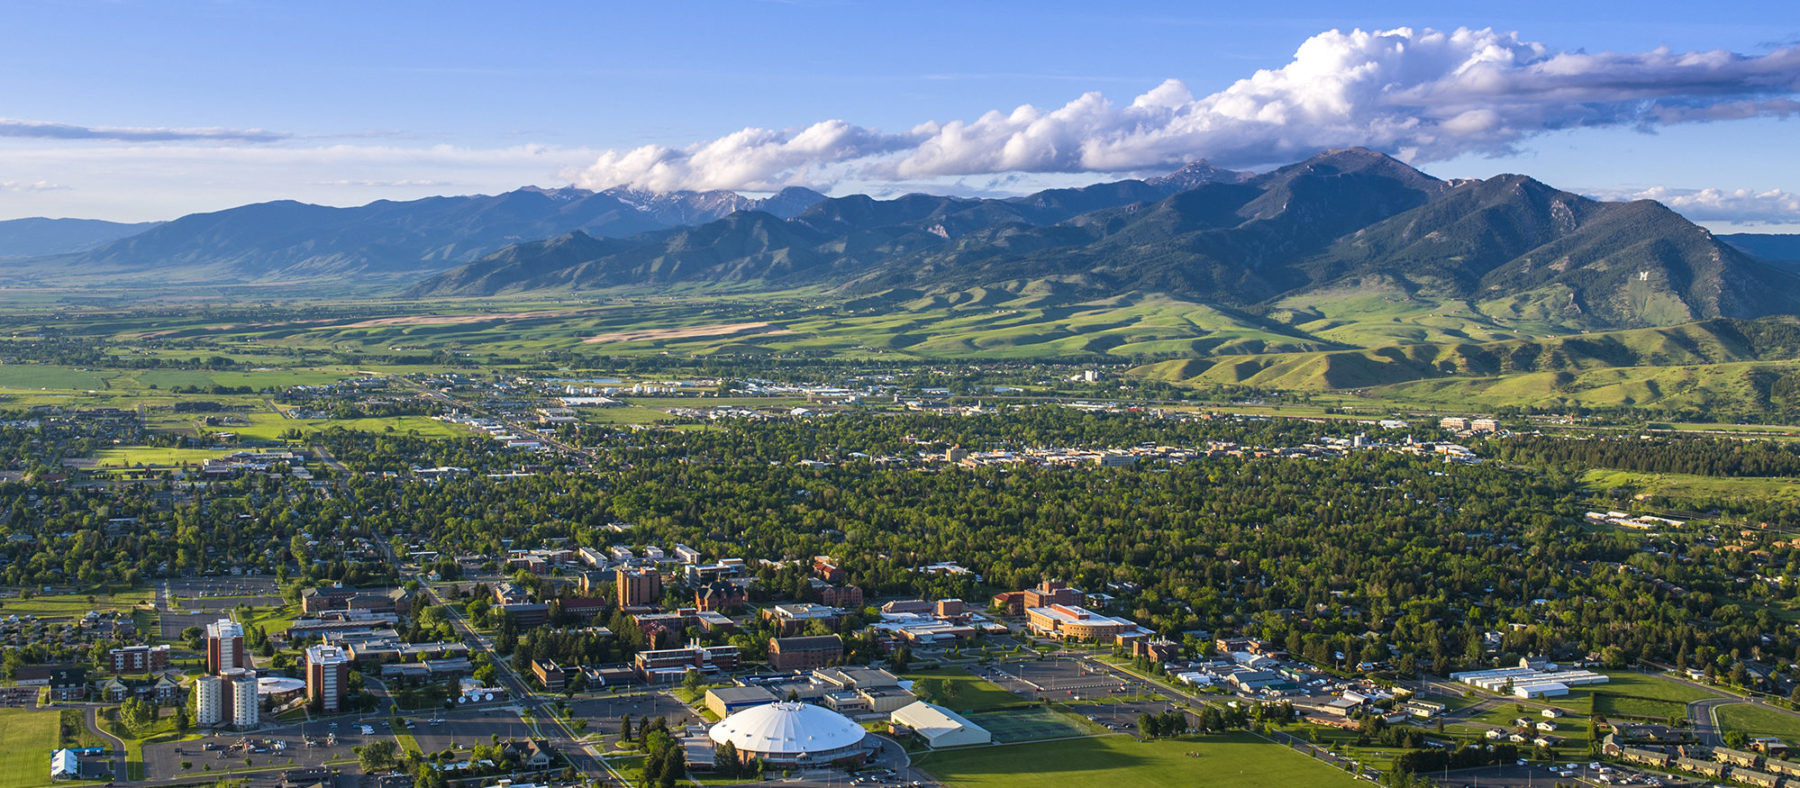
\includegraphics[width=5in,height=\textheight]{images/msu-campus.jpg}}
\usepackage{etoolbox}
\makeatletter
\providecommand{\subtitle}[1]{% add subtitle to \maketitle
  \apptocmd{\@title}{\par {\large #1 \par}}{}{}
}
\makeatother
\subtitle{Spring 2025\\
Montana State University}
\author{Melinda Yager\\
Jade Schmidt\\
Stacey Hancock}
\date{}

\begin{document}
\maketitle

\newpage
\thispagestyle{empty}

This resource was developed by Melinda Yager, Jade Schmidt, and Stacey Hancock in 2021 to accompany the online textbook: Hancock, S., Carnegie, N., Meyer, E., Schmidt, J., and Yager, M. (2021). \emph{Montana State Introductory Statistics with R}. Montana State University. \url{https://mtstateintrostats.github.io/IntroStatTextbook/}.

This resource is released under a \href{https://creativecommons.org/licenses/by-nc-sa/4.0/}{Creative Commons BY-NC-SA 4.0} license unless otherwise noted.

\setcounter{tocdepth}{1}
\addtocontents{toc}{\protect\thispagestyle{empty}}
\tableofcontents
\thispagestyle{empty}

\newpage
\setcounter{page}{1}

\chapter*{Preface}\label{preface}
\addcontentsline{toc}{chapter}{Preface}

This coursepack accompanies the textbook for STAT 216: Montana State Introductory Statistics with R, which can be found at \url{https://mtstateintrostats.github.io/IntroStatTextbook/}. The syllabus for the course (including the course calendar), data sets, and links to D2L Brightspace, Gradescope, and the MSU RStudio server can be found on the course webpage: \url{https://math.montana.edu/courses/s216/}.
Other notes and review materials are linked in D2L.

Each of the activities in this workbook is designed to target specific learning outcomes of the course, giving you practice with important statistical concepts in a group setting with instructor guidance. In addition to the in-class activities for the course, video notes are provided to aid in taking notes while you complete the required videos. Bring this workbook with you to class each class period, and take notes in the workbook as you would your own notes. A well-written completed workbook will provide an optimal study guide for exams!

All activities and labs in this coursepack will be completed during class time. Parts of each lab will be turned in on Gradescope. To aid in your understanding, read through the introduction for each activity before attending class each day.

STAT 216 is a 3-credit in-person course. In our experience, it takes six to nine hours per week outside of class to achieve a good grade in this class. By ``good'' we mean at least a C because a grade of D or below does not count toward fulfilling degree requirements. Many of you set your goals higher than just getting a C, and we fully support that. You need roughly nine hours per week to review past activities, read feedback on previous assignments, complete current assignments, and prepare for the next day's class. A typical week in the life of a STAT 216 student looks like:

\begin{itemize}
\tightlist
\item
  \emph{Prior to class meeting}:

  \begin{itemize}
  \tightlist
  \item
    Read assigned sections of the textbook, using the provided reading guides to take notes on the material.
  \item
    Watch the provided videos, taking notes in the coursepack.
  \item
    Read through the introduction to the day's in-class activity.
  \item
    Read through the week's homework assignment and note any questions you may have on the content.
  \end{itemize}
\item
  \emph{During class meeting}:

  \begin{itemize}
  \tightlist
  \item
    Work through the guided activity, in-class activity or weekly lab with your classmates and instructor, taking detailed notes on your answers to each question in the activity.
  \end{itemize}
\item
  \emph{After class meeting}:

  \begin{itemize}
  \tightlist
  \item
    Complete any parts of the activity you did not complete in class.
  \item
    Review the activity solutions in the Math and Stat Center, and take notes on key points.
  \item
    Complete any remaining assigned readings for the week.
  \item
    Complete the week's homework assignment.
  \end{itemize}
\end{itemize}

\nocite{*}

\chapter{Basics of Data and Sampling Methods}\label{basics-of-data-and-sampling-methods}

\section{Vocabulary Review and Key Topics}\label{vocabulary-review-and-key-topics}

At the beginning of each module is a summary of key topics and new vocabulary terms for that module. As you read through the material in the textbook and watch the videos prior to class, look for these terms. Reference the definitions to guide your understanding.

\subsection{Key topics}\label{key-topics}

Module 1 introduces the foundations of data: observational units, types of variables, and how to collect sample data from a population of interest in a way that allows us to generalize our results back to the population.

\subsection{Vocabulary}\label{vocabulary}

\begin{itemize}
\item
  \textbf{Data}: observations used to answer research questions.
\item
  \textbf{Observational units (cases)}: the subjects or entities on which data are collected.

  \begin{itemize}
  \tightlist
  \item
    The rows in a data set represent the observational units.
  \end{itemize}
\item
  \textbf{Sample size}: the number of observational units in a data set, denoted by \(n\).
\item
  \textbf{Variable}: the characteristics collected on each observational unit.
\item
  \textbf{Types of variables}:

  \begin{itemize}
  \item
    \textbf{Categorical}: cases are grouped into categories.
  \item
    \textbf{Quantitative}: numerical measurements, where performing arithmetic operations makes sense.
  \end{itemize}
\item
  \textbf{Target population}: group of observational units of interest.
\item
  \textbf{Sample}: subset of the population.
\item
  \textbf{Sampling methods}:

  \begin{itemize}
  \item
    \textbf{Unbiased sampling method (e.g., a random sample)}: on average, the sample will be representative of the target population; all observational units in the target population have the same chance of being selected.
  \item
    \textbf{Biased sampling method (e.g., convenience sample)}: on average, the sample will not be representative of the target population; some part of the target population will be over- or under-represented.
  \end{itemize}
\item
  \textbf{Type of sampling bias}:

  \begin{itemize}
  \item
    \textbf{Selection bias}: method of sampling is biased; some part of the target population is over- or under-represented.
  \item
    \textbf{Non-response bias}: part of a pre-selected sample does not respond or cannot be reached.
  \item
    \textbf{Response bias}: responses are not truthful (poor/leading question phrasing, social desirability).
  \end{itemize}
\end{itemize}

\newpage

\begin{itemize}
\item
  \textbf{Generalization}: to what group of observational units can the results be applied to?

  \begin{itemize}
  \item
    If an unbiased method of selection was used and there is no non-response or response bias, we can generalize the results to the target population.
  \item
    If a biased method of selection was used or if non-response or response bias is present, we can only generalize the result to the sample or similar observational units.
  \end{itemize}
\end{itemize}

\newpage

\section{Activity 1: Intro to Data}\label{activity-1-intro-to-data}

\setstretch{1}

\subsection{Learning outcomes}\label{learning-outcomes}

\begin{itemize}
\tightlist
\item
  Creating a data set
\end{itemize}

\subsection{Terminology review}\label{terminology-review}

Statistics is the study of how best to collect, analyze, and draw conclusions from data. This week in class you will be introduced to the following terms:

\begin{itemize}
\item
  Observational units or cases
\item
  Variables: categorical or quantitative
\end{itemize}

For more on these concepts, read Chapter 1 in the textbook.

\subsection{General information on the Coursepack}\label{general-information-on-the-coursepack}

Information is provided throughout each activity and lab to guide students through that day's activity or lab. Be sure to read ALL the material provided at the beginning of the activity and between each question. At the end of each activity is a section called \emph{Take-home messages} that contains key points from the day's activity. Use these to review the day's activity and make sure you have a full understanding of that material.

\subsection{Steps of the statistical investigation process}\label{steps-of-the-statistical-investigation-process}

As we move through the semester we will work through the six steps of the statistical investigation process.

\begin{enumerate}
\def\labelenumi{\arabic{enumi}.}
\item
  Ask a research question.
\item
  Design a study and collect data.
\item
  Summarize and visualize the data.
\item
  Use statistical analysis methods to draw inferences from the data.
\item
  Communicate the results and answer the research question.
\item
  Revisit and look forward.
\end{enumerate}

Today we will focus on the first two steps.

\textbf{Step 1}: The first step of any statistical investigation is to \emph{ask a research question}. As stated in the textbook, ``with the rise of data science, however, we might not start with a research question, and instead start with a data set.'' Today we will create a data set by collecting responses on students in class.

\textbf{Step 2}: To answer any research question, we must \emph{design a study and collect data}. Our study will consist of answers from each student. Your responses will become our observed data that we will explore.

\textbf{Observational units} or \textbf{cases} are the subjects data are collected on. In a spreadsheet of the data set, each row will represent a single observational unit.

\newpage

\begin{enumerate}
\def\labelenumi{\arabic{enumi}.}
\tightlist
\item
  Open the Google Form linked in D2L and fill in the responses for the following questions. When creating a data set for use in R it is important to use single words or an underscore between words. Each outcome must be written the same way each time. Make sure to use all lowercase letters to create this data set to have consistency between responses. Do not give units of measure for numerical values within the data set. For \texttt{Residency} use in\_state or out\_state as the two outcomes.
\end{enumerate}

\begin{itemize}
\tightlist
\item
  Major: what is your declared major?
\end{itemize}

\vspace{0.2in}

\begin{itemize}
\tightlist
\item
  Residency: do you have in-state or out-of-state residency?
\end{itemize}

\vspace{0.2in}

\begin{itemize}
\tightlist
\item
  Num\_Credits: how many credits are you taking this semester?
\end{itemize}

\vspace{0.2in}

\begin{itemize}
\tightlist
\item
  Dominant\_hand: are you left or right-handed?
\end{itemize}

\vspace{0.2in}

\begin{itemize}
\tightlist
\item
  Hand\_span: what is the width of your dominant hand from the tip of your thumb to the tip of your pinky with your hand spread out measured in cm?
\end{itemize}

\vspace{0.2in}

\begin{itemize}
\tightlist
\item
  Grip\_dominant: what is the grip strength measured in lbs for your dominant hand?
\end{itemize}

\vspace{0.2in}

\begin{itemize}
\tightlist
\item
  Grip\_nondominant: what is the grip strength measured in lbs for your non-dominant hand?
\end{itemize}

\vspace{0.2in}

\subsection{Take-home messages}\label{take-home-messages}

\begin{enumerate}
\def\labelenumi{\arabic{enumi}.}
\item
  When creating a data set, each row will represent a single observational unit or case. Each column represents a variable collected. It is important to write each variable as a single word or use an underscore between words.
\item
  Make sure to be consistent with writing each outcome in the data set as R is case sensitive. All outcomes must be written exactly the same way.
\end{enumerate}

\subsection{Additional notes}\label{additional-notes}

Use this space to summarize your thoughts and take additional notes on today's activity and material covered, and to write down the names and contact information of your teammates.

\newpage

\section{Video Notes: Intro to data and Sampling Methods}\label{video-notes-intro-to-data-and-sampling-methods}

\setstretch{1}

Read through Sections 1.1 -- 1.3 and 2.1 in the course textbook and watch the course videos prior to coming to class. Fill in the following questions to aid in your understanding of the material. Many of the following questions are asked on the video quiz on Gradescope.

\subsection{Course Videos}\label{course-videos}

\begin{itemize}
\item
  1.2.1and1.2.2
\item
  1.2.3to1.2.4
\item
  2.1
\end{itemize}

\subsection*{Data basics: Video 1.2.1and1.2.2}\label{data-basics-video-1.2.1and1.2.2}
\addcontentsline{toc}{subsection}{Data basics: Video 1.2.1and1.2.2}

Data: \_\_\_\_\_\_\_\_\_\_\_\_\_\_\_\_\_\_\_\_\_\_\_\_\_\_\_\_\_\_\_ used to answer research questions

Observational unit or case: the people or things we \_\_\_\_\_\_\_\_\_\_\_\_\_\_\_\_\_\_\_\_\_ data from; represents the \_\_\_\_\_\_\_\_\_\_\_ in each data set

Variable: characteristics measured on each \_\_\_\_\_\_\_\_\_\_\_\_\_\_\_\_\_\_\_\_\_\_\_\_\_\_\_\_\_\_\_.

\subsubsection*{Types of variables}\label{types-of-variables}
\addcontentsline{toc}{subsubsection}{Types of variables}

\begin{itemize}
\tightlist
\item
  Categorical variable:
\end{itemize}

\vspace{0.5in}

\setstretch{1.5}

\rgi - Ordinal: levels of the variable have a natural ordering

\rgi \rgi Examples: `Scale' questions, years of schooling completed

\rgi - Nominal:levels of the variable do not have a natural ordering

\rgi \rgi Examples: hair color, eye color, zipcode

\setstretch{1}

\begin{itemize}
\tightlist
\item
  Quantitative variable:
\end{itemize}

\vspace{0.5in}

\setstretch{1.5}

\rgi - Continuous variables: value can be any value within a range.

\rgi \rgi Examples: percentage of students who are nursing majors

\rgi \rgi \rgi - average hours of exercise per week

\rgi \rgi \rgi - distance or time (measured with enough precision)

\rgi - Discrete variables: can only be specific values, with jumps between

\rgi \rgi Examples: SAT score

\rgi \rgi \rgi - number of car accidents

\setstretch{1}
\newpage

Example: The Bureau of Transportation Statistics ({``Bureau of Transportation Statistics''} 2019) collects data on all forms of public transportation. The data set seen here includes several variables collect on flights departing on a random sample of 150 US airports in December of 2019.

\vspace{1mm}

\begin{Shaded}
\begin{Highlighting}[]
\NormalTok{airport }\OtherTok{\textless{}{-}} \FunctionTok{read.csv}\NormalTok{(}\StringTok{"data/airport\_delay.csv"}\NormalTok{)}
\FunctionTok{glimpse}\NormalTok{(airport)}
\CommentTok{\#\textgreater{} Rows: 150}
\CommentTok{\#\textgreater{} Columns: 19}
\CommentTok{\#\textgreater{} $ airport             \textless{}chr\textgreater{} "ABI", "ABY", "ACV", "ACY", "ADQ", "AEX", "ALB", "\textasciitilde{}}
\CommentTok{\#\textgreater{} $ city                \textless{}chr\textgreater{} "Abilene", "Albany", "Arcata/Eureka", "Atlantic Ci\textasciitilde{}}
\CommentTok{\#\textgreater{} $ state               \textless{}chr\textgreater{} " TX", " GA", " CA", " NJ", " AK", " LA", " NY", "\textasciitilde{}}
\CommentTok{\#\textgreater{} $ airport\_name        \textless{}chr\textgreater{} " Abilene Regional", " Southwest Georgia Regional"\textasciitilde{}}
\CommentTok{\#\textgreater{} $ hub                 \textless{}chr\textgreater{} "no", "no", "no", "no", "no", "no", "no", "no", "n\textasciitilde{}}
\CommentTok{\#\textgreater{} $ international       \textless{}chr\textgreater{} "no", "no", "no", "yes", "no", "yes", "yes", "yes"\textasciitilde{}}
\CommentTok{\#\textgreater{} $ elevation\_1000      \textless{}dbl\textgreater{} 1.7906, 0.1932, 0.2223, 0.0748, 0.0787, 0.0881, 0.\textasciitilde{}}
\CommentTok{\#\textgreater{} $ latitude            \textless{}dbl\textgreater{} 32.4, 31.5, 41.0, 39.5, 57.7, 31.3, 42.7, 35.2, 45\textasciitilde{}}
\CommentTok{\#\textgreater{} $ longitude           \textless{}dbl\textgreater{} {-}99.7, {-}81.2, {-}124.1, {-}74.6, {-}152.5, {-}92.5, {-}73.8,\textasciitilde{}}
\CommentTok{\#\textgreater{} $ arr\_flights         \textless{}int\textgreater{} 195, 81, 215, 293, 54, 282, 943, 410, 53, 32314, 6\textasciitilde{}}
\CommentTok{\#\textgreater{} $ perc\_delay15        \textless{}dbl\textgreater{} 16.410256, 13.580247, 23.255814, 15.358362, 12.962\textasciitilde{}}
\CommentTok{\#\textgreater{} $ perc\_cancelled      \textless{}dbl\textgreater{} 0.5128205, 0.0000000, 4.1860465, 0.6825939, 14.814\textasciitilde{}}
\CommentTok{\#\textgreater{} $ perc\_diverted       \textless{}dbl\textgreater{} 0.00000000, 0.00000000, 2.32558139, 0.68259386, 0.\textasciitilde{}}
\CommentTok{\#\textgreater{} $ arr\_delay           \textless{}int\textgreater{} 1563, 1244, 4763, 2905, 329, 1293, 15127, 9705, 25\textasciitilde{}}
\CommentTok{\#\textgreater{} $ carrier\_delay       \textless{}int\textgreater{} 459, 890, 1613, 476, 180, 302, 5627, 2253, 439, 10\textasciitilde{}}
\CommentTok{\#\textgreater{} $ weather\_delay       \textless{}int\textgreater{} 21, 43, 549, 124, 1, 58, 2346, 168, 1236, 13331, 2\textasciitilde{}}
\CommentTok{\#\textgreater{} $ nas\_delay           \textless{}int\textgreater{} 257, 39, 154, 771, 51, 112, 2096, 616, 746, 45674,\textasciitilde{}}
\CommentTok{\#\textgreater{} $ security\_delay      \textless{}int\textgreater{} 0, 0, 0, 25, 0, 0, 44, 0, 0, 375, 0, 83, 0, 23, 0,\textasciitilde{}}
\CommentTok{\#\textgreater{} $ late\_aircraft\_delay \textless{}int\textgreater{} 826, 272, 2447, 1509, 97, 821, 5014, 6668, 108, 10\textasciitilde{}}
\end{Highlighting}
\end{Shaded}

\begin{itemize}
\tightlist
\item
  What are the observational units?
\end{itemize}

\vspace{0.2in}

\begin{itemize}
\tightlist
\item
  Identify which variables are categorical.
\end{itemize}

\vspace{0.2in}

\begin{itemize}
\tightlist
\item
  Identify which variables are quantitative.
\end{itemize}

\vspace{0.2in}

\subsubsection*{Exploratory data analysis (EDA)}\label{exploratory-data-analysis-eda}
\addcontentsline{toc}{subsubsection}{Exploratory data analysis (EDA)}

Summary statistic: a single number which \_\_\_\_\_\_\_\_\_\_\_\_\_\_\_\_\_\_\_\_\_\_\_ an entire data set

\begin{itemize}
\tightlist
\item
  Also called the point estimate.
\end{itemize}

\rgi Examples:

\rgi \rgi proportion of people who had a stroke

\vspace{0.3in}

\rgi \rgi mean (or average) age

\vspace{0.3in}

\begin{itemize}
\tightlist
\item
  The summary statistic and type of plot used depends on the type (categorical or quantitative) of variable(s)!
\end{itemize}

\newpage

\subsection*{Roles of variables: 1.2.3to1.2.4}\label{roles-of-variables-1.2.3to1.2.4}
\addcontentsline{toc}{subsection}{Roles of variables: 1.2.3to1.2.4}

Explanatory variable: predictor variable

\begin{itemize}
\item
  The variable researchers think \emph{may be} \_\_\_\_\_\_\_\_\_\_\_\_\_
  the other variable.
\item
  In an experiment, what the researchers \_\_\_\_\_\_\_\_\_\_\_\_\_ or \_\_\_\_\_\_\_\_\_\_\_\_\_\_\_\_.
\item
  The groups that we are comparing from the data set.
\end{itemize}

Response variable:

\begin{itemize}
\item
  The variable researchers think \emph{may be} \_\_\_\_\_\_\_\_\_\_\_\_\_\_\_\_\_\_\_ by the other variable.
\item
  Always simply \_\_\_\_\_\_\_\_\_\_\_\_\_\_\_\_ or \_\_\_\_\_\_\_\_\_\_\_\_\_\_\_\_\_\_; never controlled by researchers.
\end{itemize}

Examples:

Can you predict a criminal's height based on the footprint left at the scene of a crime?

\begin{itemize}
\tightlist
\item
  Identify the explanatory variable:
\end{itemize}

\vspace{0.25in}

\begin{itemize}
\tightlist
\item
  Identify the response variable:
\end{itemize}

\vspace{0.25in}

Does marking an item on sale (even without changing the price) increase the number of units sold per day, on average?

\begin{itemize}
\tightlist
\item
  Identify the explanatory variable:
\end{itemize}

\vspace{0.25in}

\begin{itemize}
\tightlist
\item
  Identify the response variable:
\end{itemize}

\vspace{0.25in}

In the Physician's Health Study ({``Physician's Health Study,''} n.d.), male physicians participated in a study to determine whether taking a daily low-dose aspirin reduced the risk of heart attacks. The male physicians were randomly assigned to the treatment groups. After five years, 104 of the 11,037 male physicians taking a daily low-dose aspirin had experienced a heart attack while 189 of the 11,034 male physicians taking a placebo had experienced a heart attack.

\begin{itemize}
\tightlist
\item
  Identify the explanatory variable:
\end{itemize}

\vspace{0.25in}

\begin{itemize}
\tightlist
\item
  Identify the response variable:
\end{itemize}

\vspace{0.25in}

\subsubsection*{Relationships between variables}\label{relationships-between-variables}
\addcontentsline{toc}{subsubsection}{Relationships between variables}

\setstretch{1.5}

\begin{itemize}
\item
  Association: the \_\_\_\_\_\_\_\_\_\_\_\_\_ between variables create a pattern; knowing something about one variable tells us about the other.

  \begin{itemize}
  \item
    Positive association: as one variable \_\_\_\_\_\_\_\_\_\_\_\_\_, the other tends to \_\_\_\_\_\_\_\_\_\_\_\_\_\_\_ also.
  \item
    Negative association: as one variable \_\_\_\_\_\_\_\_\_\_\_\_\_, the other tends to \_\_\_\_\_\_\_\_\_\_\_\_\_.
  \end{itemize}
\item
  Independent: no clear pattern can be seen between the \_\_\_\_\_\_\_\_\_\_.
\end{itemize}

\setstretch{1}

\subsection{Concept Check}\label{concept-check}

Be prepared for group discussion in the next class. One member from the table should write the answers to the following on the whiteboard.

\begin{enumerate}
\def\labelenumi{\arabic{enumi}.}
\tightlist
\item
  What is the explanatory variable in the Male Physicians study?
\end{enumerate}

\vspace{0.4in}

\begin{enumerate}
\def\labelenumi{\arabic{enumi}.}
\setcounter{enumi}{1}
\tightlist
\item
  What is the response variable in the Male Physicians study?
\end{enumerate}

\vspace{0.4in}

\setstretch{1}

\subsection*{Sampling Methods: Video 2.1}\label{sampling-methods-video-2.1}
\addcontentsline{toc}{subsection}{Sampling Methods: Video 2.1}

\setstretch{1.5}

The method used to collect data will impact

\begin{itemize}
\item
  Target population: all \_\_\_\_\_\_\_\_\_\_\_\_\_\_\_ or \_\_\_\_\_\_\_\_\_\_\_\_\_\_ of interest
\item
  Sample:\_\_\_\_\_\_\_\_\_\_\_\_\_\_\_\_ or \_\_\_\_\_\_\_\_\_\_\_\_\_\_\_\_ from which data is collected
\end{itemize}

\setstretch{1}

Example: Many high schools moved to partial or fully online schooling in Spring of 2020. Did students who graduated in 2020 tend to have a lower GPA during freshman year of college than the previous class of college freshmen? A nationally representative sample of 1000 college students who were freshmen in AY19-20 and 1000 college students who were freshmen in AY20-21 was taken to answer this question.

\begin{itemize}
\tightlist
\item
  What is the target population?
\end{itemize}

\vspace{0.2in}

\begin{itemize}
\tightlist
\item
  What is the sample?
\end{itemize}

\vspace{0.2in}

\subsubsection*{Good vs.~bad sampling}\label{good-vs.-bad-sampling}
\addcontentsline{toc}{subsubsection}{Good vs.~bad sampling}

\setstretch{1.5}

GOAL: to have a sample that is \_\_\_\_\_\_\_\_\_\_\_\_\_\_\_ of the
\_\_\_\_\_\_\_\_\_\_\_\_\_\_ \_\_\_\_\_\_\_\_\_\_\_\_\_\_\_ on the variable(s) of interest

\setstretch{1}

\begin{itemize}
\tightlist
\item
  Unbiased sample methods:
\end{itemize}

\vspace{0.5in}

\rgi \rgi Simple random sample

\begin{itemize}
\tightlist
\item
  Biased sampling method:
\end{itemize}

\vspace{0.5in}

\newpage

\subsection*{Types of Sampling Bias}\label{types-of-sampling-bias}
\addcontentsline{toc}{subsection}{Types of Sampling Bias}

\begin{itemize}
\tightlist
\item
  Selection bias:
\end{itemize}

\vspace{0.5in}

Example of Selection Bias: Newspaper article from 1936 reported that Landon won the presidential election over Roosevelt based on a poll of 10 million voters. Roosevelt was the actual winner. What was wrong with this poll? Poll was completed using a telephone survey and not all people in 1936 had a telephone. Only a certain subset of the population owned a telephone so this subset was over-represented in the telephone survey. The results of the study, showing that Landon would win, did not represent the target population of all US voters.

\begin{itemize}
\tightlist
\item
  Non-response bias:
\end{itemize}

\vspace{0.5in}

\begin{itemize}
\tightlist
\item
  To calculate the non-response rate:
\end{itemize}

\[\frac{\text{number of people who do not respond}}{\text{total number of people selected for the sample}}\times 100\%\]

\begin{itemize}
\tightlist
\item
  For non-response bias to occur must first select people to participate and then they choose not to.
\end{itemize}

Example of Non-response bias: A company randomly selects buyers to complete a review of an online purchase but some choose not to respond.

\begin{itemize}
\tightlist
\item
  Response bias:
\end{itemize}

\vspace{0.5in}

Example of Response Bias: Police officer pulls you over and asks if you have been drinking. Expect people to say no, whether they have been drinking or not.

\begin{itemize}
\tightlist
\item
  Need to be able to predict how people will respond.
\end{itemize}

Words of caution:

\begin{itemize}
\tightlist
\item
  Convenience samples: gathering data for those who are easily
  accessible; online polls
\end{itemize}

\setstretch{1.5}

\rgi \rgi Selection bias?

\rgi \rgi Non-response bias?

\rgi \rgi Response bias?

\begin{itemize}
\tightlist
\item
  Random sampling reduces \_\_\_\_\_\_\_\_\_\_\_\_\_\_\_\_\_ bias, but
  has no impact on \_\_\_\_\_\_\_\_\_\_\_\_\_\_\_\_ or \_\_\_\_\_\_\_\_\_\_\_\_\_\_ bias.
\end{itemize}

\setstretch{1}

\newpage

\subsubsection*{Video Example}\label{video-example}
\addcontentsline{toc}{subsubsection}{Video Example}

A radio talk show asks people to phone in their views on whether the United States should pay off its debt to the United Nations.

\begin{itemize}
\tightlist
\item
  Selection?
\end{itemize}

\vspace{0.25in}

\begin{itemize}
\tightlist
\item
  Non-response?
\end{itemize}

\vspace{0.25in}

\begin{itemize}
\tightlist
\item
  Response?
\end{itemize}

\vspace{0.25in}

The Wall Street Journal plans to make a prediction for the US presidential election based on a survey of its readers and plans to follow-up to ensure everyone responds.

\begin{itemize}
\tightlist
\item
  Selection?
\end{itemize}

\vspace{0.25in}

\begin{itemize}
\tightlist
\item
  Non-response?
\end{itemize}

\vspace{0.25in}

\begin{itemize}
\tightlist
\item
  Response?
\end{itemize}

\vspace{0.25in}

A police detective interested in determining the extent of drug use by high school students, randomly selects a sample of high school students and interviews each one about any illegal drug use by the student during the past year.

\begin{itemize}
\tightlist
\item
  Selection?
\end{itemize}

\vspace{0.25in}

\begin{itemize}
\tightlist
\item
  Non-response?
\end{itemize}

\vspace{0.25in}

\begin{itemize}
\tightlist
\item
  Response?
\end{itemize}

\vspace{0.25in}

\subsection{Concept Check}\label{concept-check-1}

Be prepared for group discussion in the next class. One member from the table should write the answers to the following on the whiteboard.

\begin{enumerate}
\def\labelenumi{\arabic{enumi}.}
\tightlist
\item
  What are the two types of variables?
\end{enumerate}

\vspace{0.3in}

\begin{enumerate}
\def\labelenumi{\arabic{enumi}.}
\setcounter{enumi}{1}
\item
  Purpose of random selection:
  \vspace{0.6in}
\item
  Types of sampling bias:
\end{enumerate}

\vspace{0.5in}

\newpage

\section{Activity 2: Intro to Data Analysis and Sampling Bias}\label{activity-2-intro-to-data-analysis-and-sampling-bias}

\setstretch{1}

\subsection{Learning outcomes}\label{learning-outcomes-1}

\begin{itemize}
\item
  Identify observational units, variables, and variable types in a statistical study.
\item
  Creating a data set
\item
  Identify biased sampling methods.
\end{itemize}

\subsection{Terminology review}\label{terminology-review-1}

Statistics is the study of how best to collect, analyze, and draw conclusions from data. This week in class you will be introduced to the following terms:

\begin{itemize}
\item
  Observational units or cases
\item
  Variables: categorical or quantitative
\end{itemize}

For more on these concepts, read Chapter 1 in the textbook.

\subsubsection*{Further analysis of class data set}\label{further-analysis-of-class-data-set}
\addcontentsline{toc}{subsubsection}{Further analysis of class data set}

\begin{enumerate}
\def\labelenumi{\arabic{enumi}.}
\tightlist
\item
  What are the observational units or cases for the data collected in class on day 1?
\end{enumerate}

\vspace{0.3in}

\begin{enumerate}
\def\labelenumi{\arabic{enumi}.}
\setcounter{enumi}{1}
\tightlist
\item
  How many observations are reported in the data set? This is the \textbf{sample size}.
\end{enumerate}

\vspace{0.3in}

\begin{enumerate}
\def\labelenumi{\arabic{enumi}.}
\setcounter{enumi}{2}
\tightlist
\item
  The header for each column in the data set describes each variable measured on the observational unit. For each column of data, fill in the following table identifying the type of each variable, and if the variable is categorical whether the variables is binary and if the variable is quantitative the units of measure used.
\end{enumerate}

\begin{center}
\begin{tabular}{|l|p{1.5in}|p{0.5in}|p{0.5in}|} \hline
Column & Type of Variable & Binary? & Units? \\ \hline
Major & & &\\
& & & \\ \hline
Residency & & & \\
& & & \\ \hline
Num Credits & & & \\
& & & \\ \hline
Dominant hand & & & \\
& & & \\ \hline
Hand Span & & & \\
& & & \\ \hline
Grip strength dominant hand & & & \\
& & & \\ \hline
Grip strength non-dominant hand & & & \\
& & & \\ \hline
\end{tabular}
\end{center}

\newpage

\begin{enumerate}
\def\labelenumi{\arabic{enumi}.}
\setcounter{enumi}{3}
\tightlist
\item
  Review the completed data set with your table. Remember that when creating a data set for use in R it is important to use single words or an underscore between words. Each outcome must be written the same way each time to have consistency between responses. Do not include units of measure in the data set when reporting numerical values. Write down some issues found with the created class data set.
\end{enumerate}

\vspace{2.5in}

\subsection{Sampling Methods}\label{sampling-methods}

Discuss the following questions with your team.

\begin{enumerate}
\def\labelenumi{\arabic{enumi}.}
\setcounter{enumi}{4}
\tightlist
\item
  Describe how the students were selected for this study.
\end{enumerate}

\vspace{1in}

\begin{enumerate}
\def\labelenumi{\arabic{enumi}.}
\setcounter{enumi}{5}
\tightlist
\item
  Can we generalize the results of this study back to all University students? All MSU students? All Stat 216 students?
\end{enumerate}

\vspace{1in}

\begin{enumerate}
\def\labelenumi{\arabic{enumi}.}
\setcounter{enumi}{6}
\tightlist
\item
  Explain your answer to question 6.
\end{enumerate}

\newpage

\subsubsection*{Types of bias}\label{types-of-bias}
\addcontentsline{toc}{subsubsection}{Types of bias}

\begin{enumerate}
\def\labelenumi{\arabic{enumi}.}
\setcounter{enumi}{7}
\item
  To determine if the proportion of out-of-state undergraduate students at Montana State University has increased in the last 10 years, a statistics instructor sent an email survey to 500 randomly selected current undergraduate students. One of the questions on the survey asked whether they had in-state or out-of-state residency. She only received 378 responses.
  \vspace{0.1in}

  Sample size:
  \vspace{0.3in}

  Observational units sampled:
  \vspace{0.3in}

  Target population:
  \vspace{0.3in}

  Justify why there is non-response bias in this study.
  \vspace{0.5in}

  Variables measured and their types:
\end{enumerate}

\vspace{0.5in}

\begin{enumerate}
\def\labelenumi{\arabic{enumi}.}
\setcounter{enumi}{8}
\item
  A television station is interested in predicting whether or not local voters will pass a referendum to legalize marijuana for adult. The TV station asks its viewers to phone in and indicate whether they are in favor or opposed to the referendum. Of the 2241 viewers who phoned in, forty-five percent were opposed to legalizing marijuana.
  \vspace{0.1in}

  Sample size:
  \vspace{0.3in}

  Observational units sampled:
  \vspace{0.3in}

  Target population:
  \vspace{0.3in}

  Justify why there is selection bias in this study.
  \vspace{0.5in}

  Variables measured and their types:
\end{enumerate}

\vspace{0.5in}

\newpage

\begin{enumerate}
\def\labelenumi{\arabic{enumi}.}
\setcounter{enumi}{9}
\item
  To gauge the interest of Bozeman City Voters in a new swimming pool, a local organization stood outside of the Bogart Pool in Bozeman, MT, during open hours. One of the questions they asked was, ``Since the Bogart Pool is in such bad repair, don't you agree that the city should fund a new pool?''
  \vspace{0.1in}

  Sample size:
  \vspace{0.3in}

  Observational units sampled:
  \vspace{0.3in}

  Target population:
  \vspace{0.3in}

  Justify why there is response bias in this study.
  \vspace{0.5in}

  Justify why there is selection bias in this study.
  \vspace{0.5in}

  Variables measured and their types:
\end{enumerate}

\vspace{0.5in}

\subsection{Take-home messages}\label{take-home-messages-1}

\begin{enumerate}
\def\labelenumi{\arabic{enumi}.}
\item
  There are two types of variables: categorical (groups) and quantitative (numerical measures).
\item
  We will learn more about summarizing variable later in the semester. Categorical variables are summarized by calculating a proportion from the data and quantitative variables are summarized by finding the mean and the standard deviation.
\item
  There are three types of bias to be aware of when designing a sampling method: selection bias, non-response bias, and response bias.
\end{enumerate}

\subsection{Additional notes}\label{additional-notes-1}

Use this space to summarize your thoughts and take additional notes on today's activity and material covered, and to write down the names and contact information of your teammates.

\newpage

\section{Activity 3: American Indian Address}\label{activity-3-american-indian-address}

\setstretch{1}

\subsection{Learning outcomes}\label{learning-outcomes-2}

\begin{itemize}
\item
  Explain why a sampling method is unbiased or biased.
\item
  Identify biased sampling methods.
\item
  Explain the purpose of random selection and its effect on scope of inference.
\end{itemize}

\subsection{Terminology review}\label{terminology-review-2}

In this activity, we will examine unbiased and biased methods of sampling. Some terms covered in this activity are:

\begin{itemize}
\item
  Random sample
\item
  Unbiased vs biased methods of selection
\item
  Generalization
\end{itemize}

To review these concepts, see Chapter 2 in the textbook.

\subsection{Class Preparation}\label{class-preparation}

Prior to the next class, complete questions 1--3.

\subsection{American Indian Address}\label{american-indian-address}

For this activity, you will read a speech given by Jim Becenti, a member of the Navajo American Indian tribe, who spoke about the employment problems his people faced at an Office of Indian Affairs meeting in Phoenix, Arizona, on January 30, 1947 (Moquin and Van Doren 1973). His speech is below:

\textbf{It is hard for us to go outside the reservation where we meet strangers. I have been off the reservation ever since I was sixteen. Today I am sorry I quit the Santa Fe {[}Railroad{]}. I worked for them in 1912--13. You are enjoying life, liberty, and happiness on the soil the American Indian had, so it is your responsibility to give us a hand, brother. Take us out of distress. I have never been to vocational school. I have very little education. I look at the white man who is a skilled laborer. When I was a young man I worked for a man in Gallup as a carpenter's helper. He treated me as his own brother. I used his tools. Then he took his tools and gave me a list of tools I should buy and I started carpentering just from what I had seen. We have no alphabetical language.}

\textbf{We see things with our eyes and can always remember it. I urge that we help my people to progress in skilled labor as well as common labor. The hope of my people is to change our ways and means in certain directions, so they can help you someday as taxpayers. If not, as you are going now, you will be burdened the rest of your life. The hope of my people is that you will continue to help so that we will be all over the United States and have a hand with you, and give us a brotherly hand so we will be happy as you are. Our reservation is awful small. We did not know the capacity of the range until the white man come and say ``you raise too much sheep, got to go somewhere else,'' resulting in reduction to a skeleton where the Indians can't make a living on it. For eighty years we have been confused by the general public, and what is the condition of the Navajo today? Starvation! We are starving for education. Education is the main thing and the only thing that is going to make us able to compete with you great men here talking to us.}

\subsubsection*{By eye selection}\label{by-eye-selection}
\addcontentsline{toc}{subsubsection}{By eye selection}

\begin{enumerate}
\def\labelenumi{\arabic{enumi}.}
\tightlist
\item
  Circle ten words in Jim Becenti's speech which are a representative sample of the length of words in the entire text. Describe your method for selecting this sample.
\end{enumerate}

\vspace{0.3in}

\begin{enumerate}
\def\labelenumi{\arabic{enumi}.}
\setcounter{enumi}{1}
\tightlist
\item
  Fill in the table below with your selected words from the previous question and the length of each word (number of letters/digits in the word):
  \vspace{1mm}
\end{enumerate}

\begin{center}
\begin{tabular}{|l|p{3in}|p{1in}|} \hline
Observation & Word & Length  \\ \hline
1 & & \\ 
& & \\ \hline
2 & & \\ 
& & \\ \hline
3 & & \\ 
& & \\ \hline
4 & & \\ 
& & \\ \hline
5 & & \\ 
& & \\ \hline
6 & & \\ 
& & \\ \hline
7 & & \\
& & \\ \hline
8 & & \\ 
& & \\ \hline
9 & & \\ 
& & \\ \hline
10 & & \\ 
& & \\ \hline
\end{tabular}
\end{center}

\begin{enumerate}
\def\labelenumi{\arabic{enumi}.}
\setcounter{enumi}{2}
\tightlist
\item
  Calculate the mean (average) word length in your selected sample. Is this value a parameter or a statistic?\\
  \vspace{0.3in}
\end{enumerate}

\subsection{Class Activity}\label{class-activity}

\begin{enumerate}
\def\labelenumi{\arabic{enumi}.}
\tightlist
\item
  Report your mean word length in the Google sheet. Your instructor will create a visualization of the distribution of results generated by your class. Draw a picture of the plot here. Include a descriptive \(x\)-axis label. Report the mean of the sample mean word lengths.
\end{enumerate}

\vspace{2in}

\newpage

\begin{enumerate}
\def\labelenumi{\arabic{enumi}.}
\setcounter{enumi}{1}
\tightlist
\item
  Calculate how far your sample mean from Q1 is from the mean of the sample mean word lengths. Report this difference in the Google sheet. Your instructor will show you how to calculate the standard deviation.
\end{enumerate}

\vspace{1in}

~~~Interpret the standard deviation of the statistics in context of the problem.

\vspace{0.8in}

The plot created in the question 1 is a sampling distribution of statistics. This sampling distribution plots the mean word length from many samples taken from the population of words.

\begin{enumerate}
\def\labelenumi{\arabic{enumi}.}
\setcounter{enumi}{2}
\item
  Based on the plot and summary statistics of the sample mean word lengths, what is your best guess for the average word length of the population of all 359 words in the speech?
  \vspace{0.3in}
\item
  The true mean word length of the population of all 359 words in the speech is 3.95 letters. Is this value a parameter or a statistic?\\
  \vspace{0.2in}

  Where does the value of 3.95 fall in the plot given? Near the center of the distribution? In the tails of the distribution?
  \vspace{0.3in}
\item
  If the class samples were truly representative of the population of words, what proportion of sample means in the sampling distribution would you expect to be below 3.95?
  \vspace{0.5in}
\item
  Using the graph in Q1, estimate the proportion of students' computed sample means that were lower than the true mean of 3.95 letters?
  \vspace{0.5in}
\item
  Based on your answers to questions 5 and 6, would you say the sampling method used by the class is biased or unbiased? Justify your answer.\\
  \vspace{0.5in}
\item
  If the sampling method is biased, what type of sampling bias (selection, response, non-response) is present? What is the direction of the bias, i.e., does the method tend to overestimate or underestimate the population mean word length?
  \vspace{0.5in}
\item
  Should we use results from our ``by eye'' samples to make a statement about the word length in the population of words in Becenti's address? Why or why not?
  \vspace{0.6in}
\end{enumerate}

\subsubsection*{Random selection}\label{random-selection}
\addcontentsline{toc}{subsubsection}{Random selection}

Suppose instead of attempting to select a representative sample by eye (which did not work), each student used a random number generator to select a simple random sample of 10 words. A \textbf{simple random sample} relies on a random mechanism to choose a sample, without replacement, from the population, such that every sample of size 10 is equally likely to be chosen.

To use a random number generator to select a simple random sample, you first need a numbered list of all the words in the population, called a \textbf{sampling frame}. You can then generate 10 random numbers from the numbers 1 to 359 (the number of words in the population), and the chosen random numbers correspond to the chosen words in your sample.

\begin{enumerate}
\def\labelenumi{\arabic{enumi}.}
\setcounter{enumi}{9}
\tightlist
\item
  Use the random number generator at \url{https://istats.shinyapps.io/RandomNumbers/} to select a simple random sample from the population of all 359 words in the speech.
\end{enumerate}

\begin{itemize}
\item
  Set ``Choose Minimum'' to 1 and ``Choose Maximum'' to 359 to represent the 359 words in the population (the sampling frame).
\item
  Set ``How many numbers do you want to generate?'' to 10 and ensure the ``No'' option is selected under ``Sample with Replacement?''
\item
  Click ``Generate''.
\end{itemize}

Fill in the table below with the random numbers selected and use the Becenti.csv data file found on D2L to determine each number's corresponding word and word length (number of letters/digits in the word):

\begin{center}
\begin{tabular}{|l|l|p{1in}|} \hline
Observation & Number & Length  \\ \hline
1 & & \\ 
& & \\ \hline
2 & & \\ 
& & \\ \hline
3 & & \\ 
& & \\ \hline
4 & & \\ 
& & \\ \hline
5 & & \\ 
& & \\ \hline
6 & & \\ 
& & \\ \hline
7 & & \\
& & \\ \hline
8 & & \\ 
& & \\ \hline
9 & &\\ 
& & \\ \hline
10 & & \\ 
& & \\ \hline
\end{tabular}
\end{center}

\newpage

\begin{enumerate}
\def\labelenumi{\arabic{enumi}.}
\setcounter{enumi}{10}
\item
  Calculate the mean word length in your selected sample in question 10. Is this value a parameter or a statistic?
  \vspace{0.3in}
\item
  Report your mean word length in the Google sheet. Your instructor will create a visualization of the distribution of results generated by your class. Draw a picture of the plot here. Include a descriptive \(x\)-axis label. Report the mean and standard deviation of the data.
\end{enumerate}

\vspace{2.25in}

\begin{enumerate}
\def\labelenumi{\arabic{enumi}.}
\setcounter{enumi}{12}
\item
  Where does the value 3.95, the true mean word length, fall in the distribution given? Near the center of the distribution? In the tails of the distribution? Circle this value on the provided distribution.
  \vspace{0.3in}
\item
  How does the plot from Q12 compare to the plot generated in Q1?
\end{enumerate}

\rgi Is the shape similar?\\
\vspace{0.2in}

\rgi Is the range (smallest to largest values) similar?

\vspace{0.2in}

\rgi Is the mean of the distribution similar?

\vspace{0.2in}

\rgi Why didn't everyone get the same sample mean?
\vspace{0.4in}

\newpage

One set of randomly generated sample mean word lengths from a single class may not be large enough to visualize the distribution results. Let's have a computer generate 1,000 sample mean word lengths for us.

The following plot illustrates a sampling distribution of 1000 samples of size 10 selected at random from the sample.

\begin{center}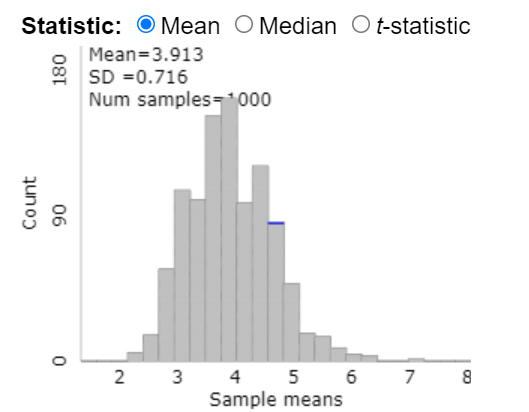
\includegraphics[width=0.75\linewidth]{images/bencenti_sampling10} \end{center}

\begin{enumerate}
\def\labelenumi{\arabic{enumi}.}
\setcounter{enumi}{14}
\item
  What is the center value (mean) of the distribution displayed above?
  \vspace{0.3in}
\item
  Explain why the sampling method of using a random number generator to generate a sample is a ``better'' method than choosing 10 words ``by eye''.
  \vspace{0.8in}
\item
  Is random selection an unbiased method of selection? Explain your answer. Be sure to reference the plot from before Q15.
  \vspace{0.5in}
\end{enumerate}

\subsection*{Effect of sample size}\label{effect-of-sample-size}
\addcontentsline{toc}{subsection}{Effect of sample size}

We will now consider the impact of sample size.

\begin{enumerate}
\def\labelenumi{\arabic{enumi}.}
\setcounter{enumi}{17}
\tightlist
\item
  First, consider if each student had selected 30 words, instead of 10, by eye. Do you think this would make the plot from the previous activity centered on 3.95 (the true mean word length)? Explain your answer.
  \vspace{0.4in}
\end{enumerate}

\newpage

Now we will select 30 words instead of 10 words at random. The following plot illustrates a sampling distribution of 1000 samples of size 30 selected at random from the sample.

\begin{center}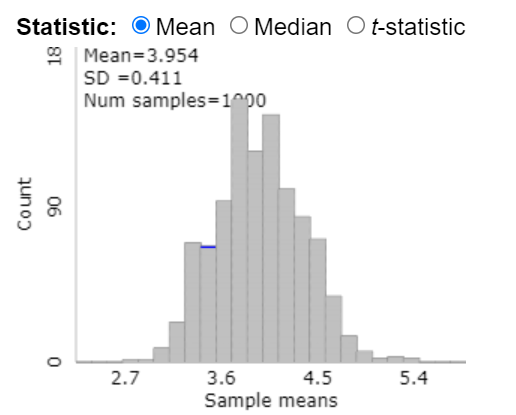
\includegraphics[width=0.75\linewidth]{images/bencenti_sampling30} \end{center}

\begin{enumerate}
\def\labelenumi{\arabic{enumi}.}
\setcounter{enumi}{18}
\tightlist
\item
  Compare the distribution displayed before question 15 to the one shown above.
\end{enumerate}

\rgi Is the shape similar?\\
\vspace{0.2in}

\rgi Is the range (smallest to largest values) similar?

\vspace{0.2in}

\rgi Is the mean of the distribution similar?

\vspace{0.2in}

\begin{enumerate}
\def\labelenumi{\arabic{enumi}.}
\setcounter{enumi}{19}
\item
  Compare the values of the standard deviation of the plots before question 15 and before question 19. Which plot shows the smallest standard deviation?
  \vspace{0.4in}
\item
  Using the evidence from your simulations, answer the following research questions:
\end{enumerate}

\rgi Does changing the sample size impact whether the sample estimates are unbiased? Explain your answer.
\vspace{0.5in}

\rgi Does changing the sample size impact the variability (spread) of sample estimates? Explain your answer
\vspace{0.5in}

\begin{enumerate}
\def\labelenumi{\arabic{enumi}.}
\setcounter{enumi}{21}
\tightlist
\item
  What is the purpose of random selection of a sample from the population?
\end{enumerate}

\vspace{0.8in}

\subsection{Take-home messages}\label{take-home-messages-2}

\begin{enumerate}
\def\labelenumi{\arabic{enumi}.}
\item
  When we use a biased method of selection, we will over or underestimate the parameter.
\item
  If the sampling method is biased, inferences made about the population based on a sample estimate will not be valid.
\item
  Random selection is an unbiased method of selection.
\item
  To determine if a sampling method is biased or unbiased, we compare the distribution of the estimates to the true value. We want our estimate to be on target or unbiased. When using unbiased methods of selection, the mean of the distribution matches or is very similar to our true parameter.
\item
  Random selection eliminates selection bias. However, random selection will not eliminate response or non-response bias.
\item
  The larger the sample size, the more similar (less variable) the statistics will be from different samples.
\item
  Sample size has no impact on whether a \emph{sampling method} is biased or not. Taking a larger sample using a biased method will still result in a sample that is not representative of the population.
\end{enumerate}

\subsection{Additional notes}\label{additional-notes-2}

Use this space to summarize your thoughts and take additional notes on today's activity and material covered.

\newpage

\chapter{Probability}\label{probability}

\section{Vocabulary Review and Key Topics}\label{vocabulary-review-and-key-topics-1}

\subsection{Key topics}\label{key-topics-1}

Module 2 introduces the concept of probability as a long-run relative frequency and demonstrates how to use hypothetical two-way tables to set up a probability problem and solve for unconditional and conditional probabilities.

\subsection{Vocabulary}\label{vocabulary-1}

\begin{itemize}
\item
  \textbf{Probability} (of an event): the long-run proportion of times the event would occur if the random process were repeated indefinitely (under identical conditions).
\item
  \textbf{Conditional probability} (of an event \emph{given} another event): probability of an event calculated dependent on another event having occurred.
\item
  \textbf{Probability notation}:

  \begin{itemize}
  \item
    \(P(A)\): the probability of event \(A\).

    \begin{itemize}
    \tightlist
    \item
      This is the probability of a single event, \emph{unconditional} probability calculated out of the overall population.
    \end{itemize}
  \item
    \(P(A^C)\): the probability of the \textbf{complement} of event \(A\), or ``\(A\) complement''.

    \begin{itemize}
    \item
      This is the probability of the opposite of event \(A\), or ``not \(A\)''.
    \item
      \(P(A^C) = 1 - P(A)\)
    \end{itemize}
  \item
    \(P(A\text{ and }B)\): the probability of event \(A\) and \(B\).

    \begin{itemize}
    \tightlist
    \item
      The is the probability of an ``and'' event, \emph{unconditional} probability calculated out of the overall population.
    \end{itemize}
  \item
    \(P(A|B)\): the probability of event \(A\) given (conditional on) event \(B\).

    \begin{itemize}
    \tightlist
    \item
      This is a \emph{conditional} probability calculated out of the total population for which event \(B\) occurred.
    \end{itemize}
  \end{itemize}
\end{itemize}

\newpage

\section{Video Notes: Probability}\label{video-notes-probability}

Read Chapters 23 in the course textbook. Use the following videos to complete the video notes for Module 12.

\subsection{Course Videos}\label{course-videos-1}

\begin{itemize}
\tightlist
\item
  Chapter23
\end{itemize}

\setstretch{1}

\subsection*{Probability}\label{probability-1}
\addcontentsline{toc}{subsection}{Probability}

Example: Two variables were collected on a random sample of people who had ever been married; whether a person had ever smoked and whether a person had ever been divorced. The data are displayed in the following table. This survey was based on a random sample in the United States in the early 1990s, so the data should be representative of the adult population who had ever been married at that time.

\begin{itemize}
\item
  Let event D be a person has gone through a divorce
\item
  Let event S be a person smokes
\end{itemize}

\begin{center}
\begin{tabular}{|c|c|c|c|} \hline
\hspace{0.8in} & \hspace{0.35in} Has divorced \hspace{.35in} & \hspace{0.35in} Has never divorced  \hspace{0.35in} & \hspace{0.3in} Total \hspace{0.3in} \\ 
& & & \\ \hline
Smokes & 238 & 247 & 485 \\ 
& & & \\ \hline
Does not smoke & 374 & 810 & 1184 \\ 
& & & \\ \hline
Total & 612 & 1057 & 1669 \\ 
& & & \\ \hline
\end{tabular}
\end{center}
\vspace{.1in}

\begin{itemize}
\tightlist
\item
  What is the approximate probability that the person smoked?
\end{itemize}

\vspace{0.5in}

\begin{itemize}
\tightlist
\item
  What is the approximate probability that the person had ever been divorced?
\end{itemize}

\vspace{0.5in}

\begin{itemize}
\tightlist
\item
  Given that the person had been divorced, what is the probability that he or she smoked?
\end{itemize}

\vspace{0.5in}

\begin{itemize}
\tightlist
\item
  Given that the person smoked, what is the probability that he or she had been divorced?
\end{itemize}

\vspace{0.5in}

\setstretch{1.5}

\begin{itemize}
\item
  Event: something that could occur, something we want to find the probability of

  \begin{itemize}
  \tightlist
  \item
    Getting a four when rolling a fair die
  \end{itemize}
\item
  Complement: opposite of the event

  \begin{itemize}
  \tightlist
  \item
    Getting any value but a four when rolling a fair die
  \end{itemize}
\item
  The probability of an event is the \_\_\_\_\_\_\_\_\_\_\_\_\_\_ proportion of times the event would occur if the \_\_\_\_\_\_\_\_\_\_\_\_\_\_\_\_ process were repeated indefinitely.

  \begin{itemize}
  \tightlist
  \item
    For example, the probability of getting a four when rolling a fair die is \_\_\_\_\_\_\_\_\_\_\_.
  \end{itemize}
\item
  Unconditional probabilities

  \begin{itemize}
  \item
    An \_\_\_\_\_\_\_\_\_\_\_\_\_\_\_\_\_\_\_\_probability is calculated from the entire population not\_\_\_\_\_\_\_\_\_\_\_\_\_\_\_\_\_\_\_\_\_\_\_\_\_\_\_\_\_
    on the occurrence of another event.
  \item
    Examples:

    \begin{itemize}
    \item
      The probability of a single event

      \begin{itemize}
      \tightlist
      \item
        The probability a selected Stat 216 student is a computer science major.
      \end{itemize}
    \item
      An ``And'' probability

      \begin{itemize}
      \tightlist
      \item
        The probability a selected Stat 216 student is a computer science major and a freshman.
      \end{itemize}
    \end{itemize}
  \end{itemize}
\item
  Conditional probabilities

  \begin{itemize}
  \item
    A \_\_\_\_\_\_\_\_\_\_\_\_\_\_\_\_\_\_\_\_\_ probability is calculated
    \_\_\_\_\_\_\_\_\_\_\_\_\_\_\_\_\_\_\_\_\_\_\_ on the occurrence of another event.
  \item
    Examples:

    \begin{itemize}
    \item
      The probability of event A given B

      \begin{itemize}
      \tightlist
      \item
        The probability a selected freshman Stat 216 student is a computer science major.
      \end{itemize}
    \item
      The probability of event B given A

      \begin{itemize}
      \tightlist
      \item
        The probability a selected computer science Stat 216 student is a freshman
      \end{itemize}
    \end{itemize}
  \end{itemize}
\end{itemize}

\setstretch{1}

\begin{itemize}
\item
  Let event D be a person has gone through a divorce
\item
  Let event S be a person smokes
\end{itemize}

\begin{center}
\begin{tabular}{|c|c|c|c|} \hline
\hspace{0.8in} & \hspace{0.35in} Has divorced \hspace{.35in} & \hspace{0.35in} Has never divorced  \hspace{0.35in} & \hspace{0.3in} Total \hspace{0.3in} \\ 
& & & \\ \hline
Smokes & 238 & 247 & 485 \\ 
& & & \\ \hline
Does not smoke & 374 & 810 & 1184 \\ 
& & & \\ \hline
Total & 612 & 1057 & 1669 \\ 
& & & \\ \hline
\end{tabular}
\end{center}
\vspace{.1in}

Calculate and interpret each of the following:

\setstretch{1.5}

\begin{itemize}
\tightlist
\item
  \(P(S^C)=\)
\end{itemize}

\vspace{0.6in}

\begin{itemize}
\tightlist
\item
  \(P(D^C|S^C)=\)
\end{itemize}

\vspace{0.6in}

\setstretch{1}

\setstretch{1}

\subsubsection*{Creating a hypothetical two-way table}\label{creating-a-hypothetical-two-way-table}
\addcontentsline{toc}{subsubsection}{Creating a hypothetical two-way table}

Steps:

\begin{itemize}
\item
  Start with a large number like 100000.
\item
  Then use the unconditional probabilities to fill in the row or column totals.
\item
  Now use the conditional probabilities to begin filling in the interior cells.
\item
  Use subtraction to find the remaining interior cells.
\item
  Add the column values together for each row to find the row totals.
\item
  Add the row values together for each column to find the column totals.
\end{itemize}

Example: An airline has noticed that 30\% of passengers pre-pay for checked bags at the time the ticket is purchased. The no-show rate among customers that pre-pay for checked bags is 5\%, compared to 15\% among customers that do not pre-pay for checked bags.

\begin{itemize}
\tightlist
\item
  Let event B = customer pre-pays for checked bag
\item
  Let event N = customer no shows
\end{itemize}

\setstretch{1.5}

Start by identifying the probability notation for each value given.

\begin{itemize}
\tightlist
\item
  0.30 =
\end{itemize}

\vspace{0.1in}

\begin{itemize}
\tightlist
\item
  0.05 =
\end{itemize}

\vspace{0.1in}

\begin{itemize}
\tightlist
\item
  0.15 =
\end{itemize}

\vspace{0.1in}

\setstretch{1}

\begin{center}
\begin{tabular}{|c|c|c|c|} \hline
\hspace{0.8in} & \hspace{0.35in} $B$ \hspace{.35in} & \hspace{0.35in} $B^C$  \hspace{0.35in} & \hspace{0.3in} Total \hspace{0.3in} \\ 
& & & \\ \hline
$N$& & & \\ 
& & & \\ \hline
$N^C$& & & \\ 
& & & \\ \hline
Total & & & 100,000 \\ 
& & & \\ \hline
\end{tabular}
\end{center}
\vspace{.1in}

\begin{itemize}
\tightlist
\item
  What is the probability that a randomly selected customer who shows for the flight, pre-purchased checked bags?
\end{itemize}

\vspace{1in}

\subsubsection*{Diagnostic tests}\label{diagnostic-tests}
\addcontentsline{toc}{subsubsection}{Diagnostic tests}

\begin{itemize}
\tightlist
\item
  Sensitivity:
\end{itemize}

\vspace{0.3in}

\begin{itemize}
\tightlist
\item
  Specificity:
\end{itemize}

\vspace{0.3in}

\begin{itemize}
\tightlist
\item
  Prevalence:
\end{itemize}

\vspace{0.3in}

\subsection{Concept Check}\label{concept-check-2}

Be prepared for group discussion in the next class. One member from the table should write the answers to the following on the whiteboard.

\begin{enumerate}
\def\labelenumi{\arabic{enumi}.}
\tightlist
\item
  Calculate and interpret the following: \(P(D^C|S^C)=\).
\end{enumerate}

\vspace{1in}

\begin{enumerate}
\def\labelenumi{\arabic{enumi}.}
\setcounter{enumi}{1}
\tightlist
\item
  What is the probability notation for 0.15 in the airline example?
\end{enumerate}

\vspace{1in}

\newpage

\section{Activity 4: Probability Studies}\label{activity-4-probability-studies}

\setstretch{1}

\subsection{Learning outcomes}\label{learning-outcomes-3}

\begin{itemize}
\item
  Recognize and simulate probabilities as long-run frequencies.
\item
  Construct two-way tables to evaluate conditional probabilities.
\end{itemize}

\subsection{Terminology review}\label{terminology-review-3}

In today's activity, we will cover two-way tables and probability. Some terms covered in this activity are:

\begin{itemize}
\item
  Proportions
\item
  Probability
\item
  Conditional probability
\item
  Two-way tables
\end{itemize}

To review these concepts, see Chapter 23 in the textbook.

\subsection{Overview of probabiliy}\label{overview-of-probabiliy}

The probability of an event is the long-run proportion of times the event would occur if the random process were repeated indefinitely (under identical conditions).

To calculate the probability of an event happening:

\[\text{probability} = \frac{\text{number of ways an event can happen}}{\text{total number of possible outcomes}}\]

For example, to calculate the probability of a coin flip landing on heads; there are only two outcomes (heads or tails) and only one possibility way to land on heads.

\[P(heads) = \frac{1}{2} = 0.5\]
The figure below shows the long-run proportion of times a simulated coin flip lands on heads on the y-axis, and the number of tosses on the x-axis. Notice how the long-run proportion starts converging to 0.5 as the number of tosses increases.

\begin{figure}

{\centering 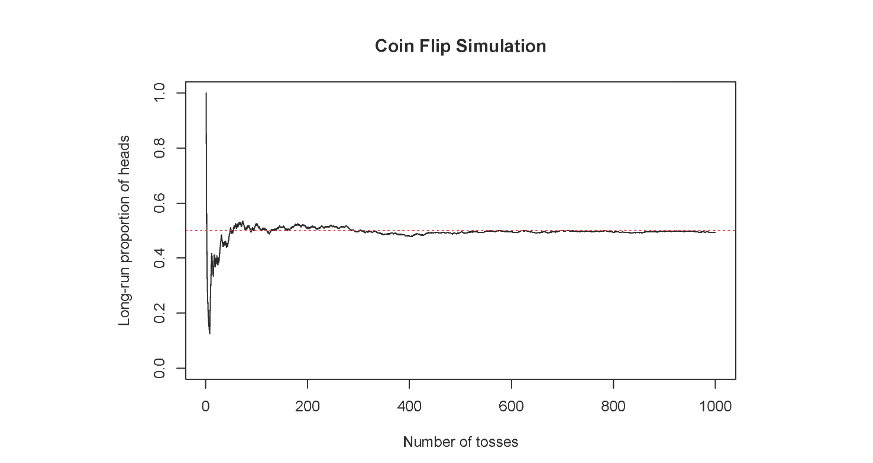
\includegraphics[width=0.65\linewidth]{images/coinsim} 

}

\end{figure}

In today's activity we will discuss the probability of a single event, the probability of an ``and'' event, and the probability of a conditional event.

\subsubsection*{Probability notation}\label{probability-notation}
\addcontentsline{toc}{subsubsection}{Probability notation}

We will use the notation P(event) to represent the probability of an event and use letters to represent events. The following are notations for different probabilities where we are discussing event A and event B:

\begin{itemize}
\item
  \(P(A)\) represents the probability of event A
\item
  \(P(A^C)\) represents the probability of the complement of event A

  \begin{itemize}
  \tightlist
  \item
    \(P(A^C) = 1 - P(A)\)
  \end{itemize}
\item
  \(P(A and B)\) represents the probability of events A and B
\item
  \(P(A|B)\) represents the probability of event A given event B
\item
  \(P(B|A)\) represents the probability of event B given event A
\end{itemize}

\subsubsection{Probability questions}\label{probability-questions}

For the beginning of this activity we will start with discussing the probabilities associated with drawing a card from a standard card deck. In a card deck there are:

\begin{itemize}
\item
  52 cards
\item
  Half are red, half are black
\item
  Four suits: spades, hearts, diamonds, and clubs
\item
  Each suit has 13 cards: cards 2--10, ace, jack, queen, and king
\item
  Let A represent the event that a card is an ace
\item
  Let B represent the event that a card is red
\end{itemize}

To find the probability of selecting an ace, first start with determining how many aces are possible (four) and how many cards will we select from (total of 52).

\vspace{1in}

Find the probability of selecting a card that is not an ace. This is the complement of event A.

\vspace{1in}

Find the probability of selecting a red ace. There are only two red aces and a total of 52 cards.

\vspace{1in}

Find the probability of selecting an ace given that the card is red. There are two red aces but only \(\frac{52}{2} = 26\) red cards

\vspace{1in}

If a card drawn is an ace, what is the probability the card drawn is red. There are four aces but only two that are red.

\vspace{1in}

\subsection{Calculating probabilities from a two-way table}\label{calculating-probabilities-from-a-two-way-table}

\begin{enumerate}
\def\labelenumi{\arabic{enumi}.}
\tightlist
\item
  In 2014, the website FiveThirtyEight examined the works of Bob Ross to see what trends could be found. They determined that of all the paintings he created, 95\% of them contained at least one ``happy tree.'' Of those works with a happy tree, 43\% contained at least one ``almighty mountain.'' Of the paintings that did not have at least one happy tree, only 10\% contained at least one almighty mountain.
  \vspace{1mm}
\end{enumerate}

Let \(A\) = Bob Ross painting contains a happy tree, and \(B\) = Bob Ross painting contains an almighty mountain
\vspace{0.1in}

\begin{center}
\begin{tabular}{|c|c|c|c|} \hline
\hspace{0.8in} & \hspace{0.25in}  $A$ \hspace{.25in} & \hspace{0.25in} $A^C$ \hspace{0.25in} & \hspace{0.25in} Total \hspace{0.25in} \\ \hline
 $B$ & 40850 & 500 & 41350 \\ \hline
 $B^C$ & 54150 & 4500 & 58650 \\ \hline
Total & 95000 & 5000 & 100000 \\ \hline
\end{tabular}
\end{center}
\vspace{.1in}

\begin{enumerate}
\def\labelenumi{\alph{enumi}.}
\tightlist
\item
  What is the probability that a randomly selected Bob Ross painting contains both a ``happy tree'' and an ``almighty mountain''? Use appropriate probability notation.
\end{enumerate}

\vspace{0.5in}

\begin{enumerate}
\def\labelenumi{\alph{enumi}.}
\setcounter{enumi}{1}
\tightlist
\item
  What is the probability that a selected Bob Ross painting without an ``almighty mountain'' contains a ``happy tree.'' Use appropriate probability notation.
\end{enumerate}

\vspace{0.5in}

\begin{enumerate}
\def\labelenumi{\alph{enumi}.}
\setcounter{enumi}{2}
\tightlist
\item
  What is the probability that a selected Bob Ross painting does not contain a ``happy tree'' given it does not contain an ``almighty mountain''. Use appropriate probability notation.
\end{enumerate}

\vspace{0.55in}

\newpage

\begin{enumerate}
\def\labelenumi{\arabic{enumi}.}
\setcounter{enumi}{1}
\item
  A recent study of population decline of white-tailed deer in Wyoming due to chronic wasting disease (Edmunds 2016) (CWD) reported the prevalence of CWD to be 35.4\%. The survival rate of CWD positive deer was 39.6\% and the survival rate of CWD negative deer was 80.1\%.\\
  \vspace{1mm}

  Let \(A\) = the event a deer has CWD, and \(B\) = the event the deer survives.
  \vspace{0.1in}

  \begin{enumerate}
  \def\labelenumii{\alph{enumii}.}
  \item
    Identify what each numerical value given in the problem represents in probability notation.
    \vspace{.1in}

    0.354 =\\
    \vspace{.1in}

    0.396 =\\
    \vspace{.1in}

    0.801 =\\
    \vspace{.1in}
  \item
    Create a hypothetical two-way table to represent the situation.
  \end{enumerate}
\end{enumerate}

\begin{center}
\begin{tabular}{|c|c|c|c|} \hline
\hspace{0.8in} & \hspace{0.35in} $A$ \hspace{.35in} & \hspace{0.35in} $A^C$  \hspace{0.35in} & \hspace{0.3in} Total \hspace{0.3in} \\ 
& & & \\ \hline
$B$& & & \\ 
& & & \\ \hline
$B^C$& & & \\ 
& & & \\ \hline
Total & & & 100,000 \\ 
& & & \\ \hline
\end{tabular}
\end{center}
\vspace{.1in}

\begin{enumerate}
\def\labelenumi{\alph{enumi}.}
\setcounter{enumi}{2}
\item
  Find \(P(A \mbox{ and } B)\). What does this probability represent in the context of the problem?
  \vspace{.8in}
\item
  Find the probability that a deer that has CWD does not survive. What is the notation used for this probability?
  \vspace{.8in}
\item
  What is the probability that a deer does not survive given they do not have CWD? What is the notation used for this probability?
\end{enumerate}

\newpage

\subsection{Take home messages}\label{take-home-messages-3}

\begin{enumerate}
\def\labelenumi{\arabic{enumi}.}
\item
  Conditional probabilities are calculated dependent on a second variable. In probability notation, the variable following \texttt{\textbar{}} is the variable on which we are conditioning. The denominator used to calculate the probability will be the total for the variable on which we are conditioning.
\item
  When creating a two-way table we typically want to put the explanatory variable on the columns of the table and the response variable on the rows.
\item
  To fill in the two-way table, always start with the unconditional variable in the total row or column and then use the conditional probabilities to fill in the interior cells.
\end{enumerate}

\subsection{Additional notes}\label{additional-notes-3}

Use this space to summarize your thoughts and take additional notes on today's activity and material covered.

\newpage

\section{Activity 5: What's the probability?}\label{activity-5-whats-the-probability}

\setstretch{1}

\subsection{Learning outcomes}\label{learning-outcomes-4}

\begin{itemize}
\item
  Recognize and simulate probabilities as long-run frequencies.
\item
  Construct two-way tables to evaluate conditional probabilities.
\end{itemize}

\subsection{Terminology review}\label{terminology-review-4}

In today's activity, we will cover two-way tables and probability. Some terms covered in this activity are:

\begin{itemize}
\item
  Proportions
\item
  Probability
\item
  Conditional probability
\item
  Two-way tables
\end{itemize}

To review these concepts, see Chapter 23 in the textbook.

\subsection{Probability}\label{probability-2}

\begin{enumerate}
\def\labelenumi{\arabic{enumi}.}
\item
  A dataset was collected on all NBA basketball players from inception of the league. The probability that an NBA player is above average height is 59.7\%. Of NBA players that are above average height, 46.4\% averaged at least four rebounds a game. The probability that an NBA player averages less than four rebounds in a game given they are below average height is 13.3\%.
  \vspace{1mm}

  Let \(A\) = player is above average height, and \(B\) = player averages at least four rebounds a game.
  \vspace{0.1in}
\end{enumerate}

\begin{center}
\begin{tabular}{|c|c|c|c|} \hline
\hspace{0.8in} & \hspace{0.25in} $A$ \hspace{.25in} & \hspace{0.25in} $A^C$ \hspace{0.25in} & \hspace{0.25in} Total \hspace{0.25in} \\ \hline $B$ & 27700.8 & 34940.1 & 62640.9 \\ \hline
 $B^C$ & 31999.2 & 5359.9 & 37359.1 \\ \hline
Total & 59700 & 40300 & 100000 \\ \hline
\end{tabular}
\end{center}
\vspace{.1in}

\begin{enumerate}
\def\labelenumi{\alph{enumi}.}
\tightlist
\item
  What is the probability that a randomly selected NBA player averages at least 4 rebounds a game? Use appropriate probability notation.
\end{enumerate}

\vspace{0.5in}

\begin{enumerate}
\def\labelenumi{\alph{enumi}.}
\setcounter{enumi}{1}
\tightlist
\item
  What is the probability that a randomly selected NBA player is both above average height and averages at least 4 rebounds a game. Use appropriate probability notation.
\end{enumerate}

\vspace{0.5in}

\begin{enumerate}
\def\labelenumi{\alph{enumi}.}
\setcounter{enumi}{2}
\tightlist
\item
  What is the probability that a randomly selected NBA player is not above average height given they do not average at least 4 rebounds a game. Use appropriate probability notation.
\end{enumerate}

\vspace{0.55in}

\newpage

\begin{enumerate}
\def\labelenumi{\arabic{enumi}.}
\setcounter{enumi}{1}
\item
  Since the early 1980s, the rapid antigen detection test (RADT) of group A \emph{streptococci} has been used to detect strep throat. A recent study of the accuracy of this test shows that the \textbf{sensitivity}, the probability of a positive RADT given the person has strep throat, is 86\% in children, while the \textbf{specificity}, the probability of a negative RADT given the person does not have strep throat, is 92\% in children. The \textbf{prevalence}, the probability of having group A strep, is 37\% in children. (Stewart et al. 2014)
  \vspace{1mm}

  Let \(A\) = the event the child has strep throat, and \(B\) = the event the child has a positive RADT.
  \vspace{0.1in}

  \begin{enumerate}
  \def\labelenumii{\alph{enumii}.}
  \item
    Identify what each numerical value given in the problem represents in probability notation.
    \vspace{.1in}

    0.86 =\\
    \vspace{.1in}

    0.92 =\\
    \vspace{.1in}

    0.37 =\\
    \vspace{.1in}
  \item
    Create a hypothetical two-way table to represent the situation.
  \end{enumerate}
\end{enumerate}

\begin{center}
\begin{tabular}{|c|c|c|c|} \hline
\hspace{0.8in} & \hspace{0.35in} $A$ \hspace{.35in} & \hspace{0.35in} $A^C$  \hspace{0.35in} & \hspace{0.3in} Total \hspace{0.3in} \\ 
& & & \\ \hline
$B$& & & \\ 
& & & \\ \hline
$B^C$& & & \\ 
& & & \\ \hline
Total & & & 100,000 \\ 
& & & \\ \hline
\end{tabular}
\end{center}
\vspace{.1in}

\begin{enumerate}
\def\labelenumi{\alph{enumi}.}
\setcounter{enumi}{2}
\item
  Find \(P(B)\). What does this probability represent in the context of the problem?
  \vspace{.8in}
\item
  Find the probability that a child with a positive RADT actually has strep throat. What is the notation used for this probability?
  \vspace{.8in}
\item
  What is the probability that a child does not have strep given that they have a positive RADT? What is the notation used for this probability?
\end{enumerate}

\newpage

\newpage

\subsection{Take home messages}\label{take-home-messages-4}

\begin{enumerate}
\def\labelenumi{\arabic{enumi}.}
\item
  Conditional probabilities are calculated dependent on a second variable. In probability notation, the variable following \texttt{\textbar{}} is the variable on which we are conditioning. The denominator used to calculate the probability will be the total for the variable on which we are conditioning.
\item
  When creating a two-way table we typically want to put the explanatory variable on the columns of the table and the response variable on the rows.
\item
  To fill in the two-way table, always start with the unconditional variable in the total row or column and then use the conditional probabilities to fill in the interior cells.
\end{enumerate}

\subsection{Additional notes}\label{additional-notes-4}

Use this space to summarize your thoughts and take additional notes on today's activity and material covered.

\newpage

\chapter{Exploring Categorical Data: Exploratory Data Analysis and Inference using Simulation-based Methods}\label{exploring-categorical-data-exploratory-data-analysis-and-inference-using-simulation-based-methods}

\section{Vocabulary Review and Key Topics}\label{vocabulary-review-and-key-topics-2}

Review the Golden Ticket posted in the resources at the end of the coursepack for a summary of a single categorical variable.

\subsection{Key topics}\label{key-topics-2}

Module 3 introduces the steps of the statistical investigation process. We conduct \textbf{exploratory data analysis} (summary statistics and plots) and simulation-based \textbf{inference} (hypothesis testing and confidence intervals) in the single categorical variable (one proportion) scenario.

\begin{itemize}
\item
  Notation for a sample proportion: \(\hat{p}\)
\item
  Notation for a population proportion: \(\pi\)
\item
  Types of plots for a single categorical variable:

  \begin{itemize}
  \item
    Frequency bar plot
  \item
    Relative frequency bar plot
  \end{itemize}
\end{itemize}

Exploratory data analysis is step 3 of the statistical investigation process. We will then use simulation-based methods \textbf{to find evidence of an effect by finding a p-value} and \textbf{estimating how large the effect is by creating a confidence interval} in the one proportion (one categorical variable) scenario. These are steps 4 and 5 from the steps of the statistical investigation process.

\subsubsection*{Steps of the statistical investigation process}\label{steps-of-the-statistical-investigation-process-1}
\addcontentsline{toc}{subsubsection}{Steps of the statistical investigation process}

As we move through the semester we will work through the six steps of the statistical investigation process.

\begin{enumerate}
\def\labelenumi{\arabic{enumi}.}
\item
  Ask a research question.
\item
  Design a study and collect data.
\item
  Summarize and visualize the data.
\item
  Use statistical analysis methods to draw inferences from the data.
\item
  Communicate the results and answer the research question.
\item
  Revisit and look forward.
\end{enumerate}

\subsection{Vocabulary}\label{vocabulary-2}

\begin{itemize}
\item
  \textbf{Summary measure}: a numerical quantity that summarizes data. Summary measures covered in STAT 216 include: single proportion, difference in proportions, single mean, paired mean difference, difference in means, correlation, and slope of a regression line.

  \begin{itemize}
  \tightlist
  \item
    For a single categorical variable, a proportion is calculated.
  \end{itemize}
\item
  \textbf{Summary statistic (point estimate)}: the value of a numerical summary measure computed from \emph{sample} data.

  \begin{itemize}
  \item
    To interpret in context include:

    \begin{itemize}
    \item
      Summary measure (in context)
    \item
      Value of the statistic
    \end{itemize}
  \end{itemize}
\item
  \textbf{Parameter of interest}: a numerical summary measure of the entire \emph{population} in which we are interested.

  \begin{itemize}
  \item
    The value of the parameter of interest is unknown (unless we have access to the entire population).
  \item
    To write in context:

    \begin{itemize}
    \item
      Population word (true, long-run, population)
    \item
      Summary measure (depends on the type of data)
    \item
      Context

      \begin{itemize}
      \item
        Observational units
      \item
        Variable(s)
      \end{itemize}
    \end{itemize}
  \end{itemize}
\item
  For a single categorical variable, the category that we are counting the proportion of is generically called a ``\textbf{success}'', with categories not a success labeled ``\textbf{failure}''. Thus, a sample proportion is the ``proportion of successes'' in the sample: the total number of successes divided by the sample size (\(n\)).
\end{itemize}

\subsubsection*{Plotting one categorical variable}\label{plotting-one-categorical-variable}
\addcontentsline{toc}{subsubsection}{Plotting one categorical variable}

\begin{itemize}
\item
  \textbf{Frequency bar plot}: plots the count (frequency) of observational units in each level of a categorical variable. R code to create a frequency bar plot:

\begin{Shaded}
\begin{Highlighting}[]
\NormalTok{object }\SpecialCharTok{\%\textgreater{}\%} \CommentTok{\# Data set piped into...}
\FunctionTok{ggplot}\NormalTok{(}\FunctionTok{aes}\NormalTok{(}\AttributeTok{x =}\NormalTok{ variable)) }\SpecialCharTok{+}   \CommentTok{\# This specifies the variable}
\FunctionTok{geom\_bar}\NormalTok{(}\AttributeTok{stat =} \StringTok{"count"}\NormalTok{) }\SpecialCharTok{+}  \CommentTok{\# Tell it to make a bar plot}
\FunctionTok{labs}\NormalTok{(}\AttributeTok{title =} \StringTok{"Don\textquotesingle{}t forget to title your plot!"}\NormalTok{,  }
   \CommentTok{\# Give your plot a title}
   \AttributeTok{x =} \StringTok{"x{-}axis label"}\NormalTok{,   }\CommentTok{\# Label the x axis}
   \AttributeTok{y =} \StringTok{"Frequency"}\NormalTok{)  }\CommentTok{\# Label the y axis}
\end{Highlighting}
\end{Shaded}
\item
  \textbf{Relative frequency bar plot}: plots the proportion (relative frequency) of observational units in each level of a categorical variable. R code to create a relative frequency bar plot:

\begin{Shaded}
\begin{Highlighting}[]
\NormalTok{object }\SpecialCharTok{\%\textgreater{}\%} \CommentTok{\# Data set piped into...}
\FunctionTok{ggplot}\NormalTok{(}\FunctionTok{aes}\NormalTok{(}\AttributeTok{x =}\NormalTok{ variable)) }\SpecialCharTok{+}   \CommentTok{\# This specifies the variable}
\FunctionTok{geom\_bar}\NormalTok{(}\FunctionTok{aes}\NormalTok{(}\AttributeTok{y =} \FunctionTok{after\_stat}\NormalTok{(prop), }\AttributeTok{group =} \DecValTok{1}\NormalTok{)) }\SpecialCharTok{+}  \CommentTok{\# Tell it to make a bar plot with proportions}
\FunctionTok{labs}\NormalTok{(}\AttributeTok{title =} \StringTok{"Don\textquotesingle{}t forget to title your plot!"}\NormalTok{,  }
   \CommentTok{\# Give your plot a title}
   \AttributeTok{x =} \StringTok{"x{-}axis label"}\NormalTok{,   }\CommentTok{\# Label the x axis}
   \AttributeTok{y =} \StringTok{"Relative Frequency"}\NormalTok{)  }\CommentTok{\# Label the y axis}
\end{Highlighting}
\end{Shaded}
\end{itemize}

\subsubsection*{Inference}\label{inference}
\addcontentsline{toc}{subsubsection}{Inference}

\begin{itemize}
\item
  \textbf{Sampling distribution} (of a statistic): the distribution of possible values of a statistic across repeated samples of the same size and under the same conditions.

  \begin{itemize}
  \tightlist
  \item
    We can create a \emph{simulated} sampling distribution using simulation-based methods to simulate many samples, or we can mathematically model the sampling distribution (theory-based methods).
  \end{itemize}
\item
  \textbf{Hypothesis testing}: a formal statistical technique for evaluating two competing possibilities about a population: the null hypothesis and alternative hypothesis.

  \begin{itemize}
  \item
    When we observe an effect in a sample, we would like to determine if this observed effect represents an actual effect in the population, or whether it was simply due to random chance.
  \item
    A hypothesis test helps us answer the following question about the population: How strong is the \emph{evidence} of an effect?
  \end{itemize}
\item
  \textbf{Null hypothesis}: typically represents a statement of ``no difference'', ``no effect'', or the status quo.

  \begin{itemize}
  \tightlist
  \item
    The null hypothesis is what we assume is true when calculating the p-value. Thus, we can never have evidence \emph{for} the null hypothesis---we cannot ``accept'' a null hypothesis---we can only find evidence \emph{against} the null hypothesis if the observed data is very unlikely to have occurred under the assumption that the null hypothesis is true.
  \end{itemize}
\item
  \textbf{Alternative hypothesis}: represents an alternative claim under consideration and is often represented by a range of possible values for the parameter of interest.

  \begin{itemize}
  \tightlist
  \item
    The alternative hypothesis is determined by the research question.
  \end{itemize}
\item
  \textbf{Hypotheses in notation for a single proportion}: In the hypotheses below, \(\pi_0\) is the \textbf{null value}.
\end{itemize}

\[H_0: \pi = \pi_0\]
\[H_A: \pi \left\{
\begin{array}{ll}
< \\
\ne \\
< \\
\end{array}
\right\}
\pi_0 \]

\begin{itemize}
\item
  \textbf{P-value}: the probability of the value of the observed sample statistic or a value more extreme, if the null hypothesis were true.

  \begin{itemize}
  \item
    To write in context include:

    \begin{itemize}
    \item
      Statement about probability or proportion of samples
    \item
      Statistic (summary measure and value)
    \item
      Direction of the alternative
    \item
      Null hypothesis (in context)
    \end{itemize}
  \end{itemize}
\item
  \textbf{Strength of evidence}: the p-value indicates the amount of evidence there is against the null hypothesis. The smaller the p-value the more evidence there is against the null hypothesis.
\end{itemize}

\begin{center}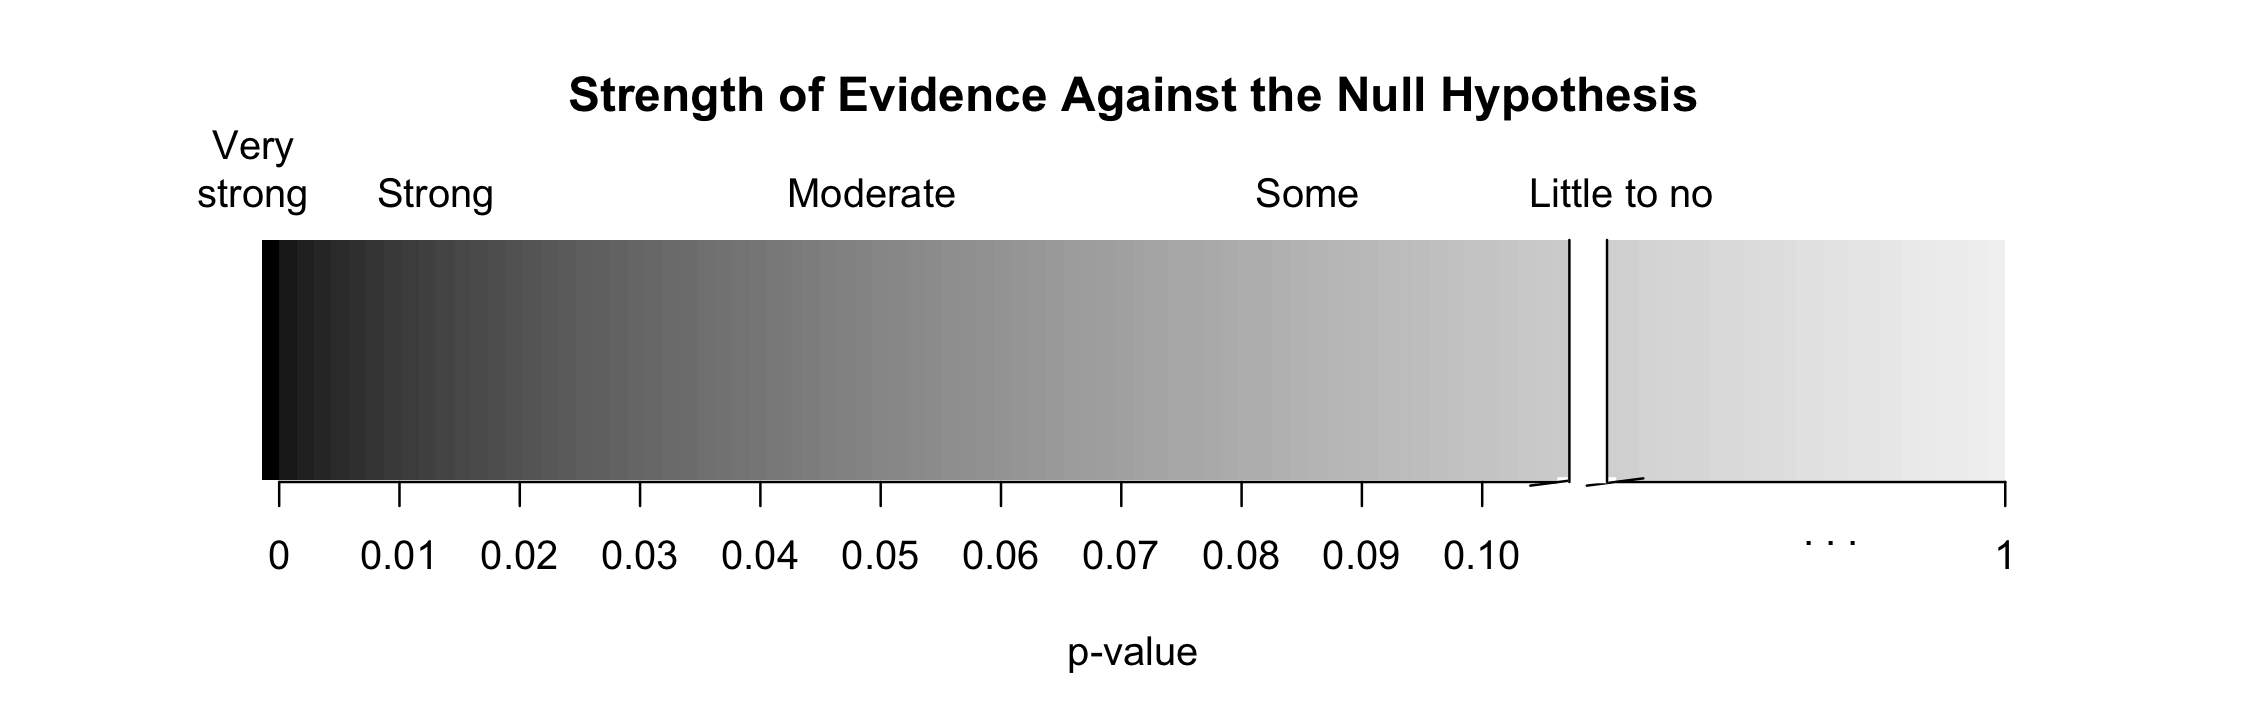
\includegraphics[width=0.9\linewidth]{images/soe_gradient_gray} \end{center}

\newpage

\begin{itemize}
\item
  \textbf{Conclusion} (to a hypothesis test): answers the research question. How much evidence is there in support of the alternative hypothesis?

  \begin{itemize}
  \item
    To write in context include:

    \begin{itemize}
    \item
      Amount of evidence
    \item
      Parameter of interest
    \item
      Direction of the alternative hypothesis
    \end{itemize}
  \end{itemize}
\item
  \textbf{Confidence interval}: an interval estimate for the parameter of interest; an interval of \emph{plausible values} for the parameter.

  \begin{itemize}
  \item
    A confidence interval helps us answer the following question about the population: How \emph{large} is the effect?
  \item
    To write in context include:

    \begin{itemize}
    \item
      How confident you are (e.g., 90\%, 95\%, 98\%, 99\%)
    \item
      Parameter of interest
    \item
      Calculated interval
    \end{itemize}
  \end{itemize}
\end{itemize}

\subsubsection{Simulation-based inference for a single proportion}\label{simulation-based-inference-for-a-single-proportion}

\begin{itemize}
\item
  \textbf{Conditions necessary to use simulation-based methods for inference for a single categorical variable}:

  \begin{itemize}
  \tightlist
  \item
    \textbf{Independence}: observational units must be independent of one another; the outcome of one observational unit should have no influence on the outcome of another.
  \end{itemize}
\item
  \textbf{Null distribution}: a sampling distribution of simulated sample statistics created under the assumption that the null hypothesis is true
\item
  \textbf{Simulation-based methods to create the null distribution}: a process of using a computer program (e.g., R) to simulate many samples that we would expect based on the null hypothesis.

  R code to use simulation methods for one categorical variable to find the p-value, \texttt{one\_proportion\_test} (from the \texttt{catstats} package), is shown below.

\begin{Shaded}
\begin{Highlighting}[]
\FunctionTok{one\_proportion\_test}\NormalTok{(}\AttributeTok{probability\_success =}\NormalTok{ xx, }\CommentTok{\# Null hypothesis value}
      \AttributeTok{sample\_size =}\NormalTok{ xx, }\CommentTok{\# Enter sample size}
      \AttributeTok{number\_repetitions =} \DecValTok{10000}\NormalTok{, }\CommentTok{\# Enter number of simulations}
      \AttributeTok{as\_extreme\_as =}\NormalTok{ xx, }\CommentTok{\# Observed statistic}
      \AttributeTok{direction =} \StringTok{"xx"}\NormalTok{, }\CommentTok{\# Specify direction of alternative hypothesis}
      \AttributeTok{summary\_measure =} \StringTok{"proportion"}\NormalTok{) }\CommentTok{\# Reporting proportion or number of successes?}
\end{Highlighting}
\end{Shaded}
\item
  \textbf{Bootstrapping}: creating a simulated sample of the same size as the original sample by sampling with replacement from the original sample.
\item
  \textbf{Simulation-based methods to create the bootstrap distribution}: a process of using a computer program to simulate many bootstrapped samples.

  R code to use simulation methods for one categorical variable to find a confidence interval, \texttt{one\_proportion\_bootstrap\_CI} (from the \texttt{catstats} package), is shown below.

\begin{Shaded}
\begin{Highlighting}[]
\FunctionTok{one\_proportion\_bootstrap\_CI}\NormalTok{(}\AttributeTok{sample\_size =}\NormalTok{ xx, }\CommentTok{\# Sample size}
                \AttributeTok{number\_successes =}\NormalTok{ xx, }\CommentTok{\# Observed number of successes}
                \AttributeTok{number\_repetitions =} \DecValTok{10000}\NormalTok{, }\CommentTok{\# Number of bootstrap samples to use}
                \AttributeTok{confidence\_level =} \FloatTok{0.95}\NormalTok{) }\CommentTok{\# Confidence level as a decimal}
\end{Highlighting}
\end{Shaded}
\item
  \textbf{Percentile method}: process to find the confidence interval from the bootstrap distribution.

  \begin{itemize}
  \item
    A 90\% confidence interval will be found between the 5th and 95th percentiles of the bootstrap distribution.
  \item
    A 95\% confidence interval will be found between the 2.5th and 97.5th percentiles of the bootstrap distribution.
  \item
    A 99\% confidence interval will be found between the 0.5th and 99.5th percentiles of the bootstrap distribution.
  \end{itemize}
\end{itemize}

\newpage

\section{Video Notes: Exploratory Data Analysis of Categorical Variables}\label{video-notes-exploratory-data-analysis-of-categorical-variables}

Read Chapter 3, 4, 9, 10 and Sections 14.1 and 14.2 in the course textbook. Use the following videos to complete the video notes for Module 4.

\subsection{Course Videos}\label{course-videos-2}

\begin{itemize}
\item
  4.1\_OneProp
\item
  4.2\_OneProp
\item
  Chapter9
\item
  14.1
\item
  Chapter10
\item
  14.2
\end{itemize}

\setstretch{1}

\subsection*{Summarizing categorical data - Video 4.1\_OneProp}\label{summarizing-categorical-data---video-4.1_oneprop}
\addcontentsline{toc}{subsection}{Summarizing categorical data - Video 4.1\_OneProp}

\begin{itemize}
\item
  A \_\_\_\_\_\_\_\_\_\_\_\_\_\_ is calculated on data from a sample
\item
  The parameter of interest is what we want to know from the population.
\item
  Includes:

  \begin{itemize}
  \item
    Population word (true, long-run, population)
  \item
    Summary measure (depends on the type of data)
  \item
    Context

    \begin{itemize}
    \item
      Observational units
    \item
      Variable(s)
    \end{itemize}
  \end{itemize}
\end{itemize}

Categorical data can be numerically summarized by calculating a \_\_\_\_\_\_\_\_\_\_\_\_\_\_\_ from the data set.

Notation used for the population proportion:

\begin{itemize}
\tightlist
\item
  Single categorical variable:
\end{itemize}

\vspace{0.2in}

Notation used for the sample proportion:

\begin{itemize}
\tightlist
\item
  Single categorical variable:
\end{itemize}

\vspace{0.2in}

\setstretch{1.5}

Categorical data can be reported in a \_\_\_\_\_\_\_\_\_\_\_\_table,
which plots counts or a \_\_\_\_\_\_\_\_\_\_\_\_\_\_
frequency table, which plots the proportion.

\setstretch{1}

\vspace{2mm}

Example from the Video: Gallatin Valley is the fastest growing county in Montana. You'll often hear Bozeman residents complaining about the `out-of-staters' moving in. A local real estate agent recorded data on a random sample of 100 home sales over the last year at her company and noted where the buyers were moving from as well as the age of the person or average age of a couple buying a home. The variable age was binned into two categories, ``Under30'' and ``Over30.'' Additionally, the variable, state the buyers were moving from, was created as a binary variable, ``Out'' for a location out of state and ``In'' for a location in state.

The following code reads in the data set, \texttt{moving\_to\_mt} and names the object moving.

\begin{Shaded}
\begin{Highlighting}[]
\NormalTok{moving }\OtherTok{\textless{}{-}} \FunctionTok{read.csv}\NormalTok{(}\StringTok{"data/moving\_to\_mt.csv"}\NormalTok{)}
\end{Highlighting}
\end{Shaded}

The \texttt{R} function \texttt{glimpse} was used to give the following output.

\begin{Shaded}
\begin{Highlighting}[]
\FunctionTok{glimpse}\NormalTok{(moving)}
\end{Highlighting}
\end{Shaded}

\begin{verbatim}
#> Rows: 100
#> Columns: 4
#> $ From      <chr> "CA", "CA", "CA", "CA", "CA", "CA", "CA", "CA", "CA", "CA", ~
#> $ Age_Group <chr> "Under30", "Under30", "Under30", "Under30", "Under30", "Unde~
#> $ Age       <int> 25, 26, 27, 27, 29, 29, 35, 37, 49, 63, 65, 77, 22, 24, 24, ~
#> $ InOut     <chr> "Out", "Out", "Out", "Out", "Out", "Out", "Out", "Out", "Out~
\end{verbatim}

\begin{itemize}
\tightlist
\item
  What are the observational units in this study?
\end{itemize}

\vspace{0.3in}

\begin{itemize}
\tightlist
\item
  What type of variable is \texttt{Age}?
\end{itemize}

\vspace{0.3in}

\begin{itemize}
\tightlist
\item
  What type of variable is \texttt{Age\_Group}?
\end{itemize}

To further analyze the categorical variable, \texttt{From}, we can create either a frequency table:

\begin{verbatim}
#>   From  n
#> 1   CA 12
#> 2   CO  8
#> 3   MT 61
#> 4   WA 19
\end{verbatim}

Or a relative frequency table:

\begin{verbatim}
#>   From  n freq
#> 1   CA 12 0.12
#> 2   CO  8 0.08
#> 3   MT 61 0.61
#> 4   WA 19 0.19
\end{verbatim}

\begin{itemize}
\tightlist
\item
  How many home sales have buyers from WA?
\end{itemize}

\vspace{0.2in}

\begin{itemize}
\tightlist
\item
  What proportion of sampled home sales have buyers from WA?
\end{itemize}

\vspace{0.2in}

\begin{itemize}
\tightlist
\item
  What notation is used for the proportion of home sale buyers that that are from WA?
\end{itemize}

\vspace{0.2in}

\subsubsection*{Displaying categorical variables - Video 4.2\_OneProp}\label{displaying-categorical-variables---video-4.2_oneprop}
\addcontentsline{toc}{subsubsection}{Displaying categorical variables - Video 4.2\_OneProp}

\begin{itemize}
\tightlist
\item
  Types of plots for a single categorical variable
\end{itemize}

\vspace{0.4in}

The following code in \texttt{R} will create a frequency bar plot of the variable, \texttt{From}.

\begin{Shaded}
\begin{Highlighting}[]
\NormalTok{moving }\SpecialCharTok{\%\textgreater{}\%}
    \FunctionTok{ggplot}\NormalTok{(}\FunctionTok{aes}\NormalTok{(}\AttributeTok{x =}\NormalTok{ From))}\SpecialCharTok{+} \CommentTok{\#Enter the variable to plot}
    \FunctionTok{geom\_bar}\NormalTok{(}\AttributeTok{stat =} \StringTok{"count"}\NormalTok{) }\SpecialCharTok{+} 
    \FunctionTok{labs}\NormalTok{(}\AttributeTok{title =} \StringTok{"Frequency Bar Plot of State of Origin for}
\StringTok{         Gallatin County Home Sales"}\NormalTok{, }
         \CommentTok{\#Title your plot (type of plot, observational units, variable)}
       \AttributeTok{y =} \StringTok{"Frequency"}\NormalTok{, }\CommentTok{\#y{-}axis label}
       \AttributeTok{x =} \StringTok{"State of Origin"}\NormalTok{) }\CommentTok{\#x{-}axis label}
\end{Highlighting}
\end{Shaded}

\begin{center}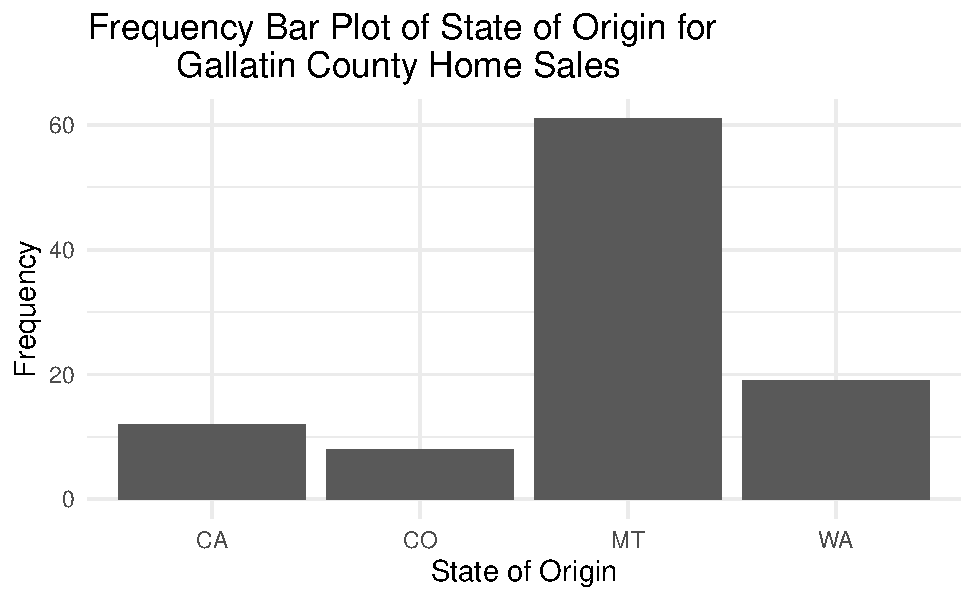
\includegraphics[width=0.65\linewidth]{03-VN03-EDA_OneCatSimulation_files/figure-latex/unnamed-chunk-5-1} \end{center}

\begin{itemize}
\tightlist
\item
  What can we see from this plot?
\end{itemize}

\vspace{0.3in}

Additionally, we can create a relative frequency bar plot.

\begin{Shaded}
\begin{Highlighting}[]
\NormalTok{moving }\SpecialCharTok{\%\textgreater{}\%}
  \FunctionTok{ggplot}\NormalTok{(}\FunctionTok{aes}\NormalTok{(}\AttributeTok{x =}\NormalTok{ From))}\SpecialCharTok{+} \CommentTok{\#Enter the variable to plot}
  \FunctionTok{geom\_bar}\NormalTok{(}\FunctionTok{aes}\NormalTok{(}\AttributeTok{y =} \FunctionTok{after\_stat}\NormalTok{(prop), }\AttributeTok{group =} \DecValTok{1}\NormalTok{)) }\SpecialCharTok{+}
  \FunctionTok{labs}\NormalTok{(}\AttributeTok{title =} \StringTok{"Relative Frequency Bar Plot of State of Origin }
\StringTok{       for Gallatin County Home Sales"}\NormalTok{, }
       \CommentTok{\#Title your plot}
       \AttributeTok{y =} \StringTok{"Relative Frequency"}\NormalTok{, }\CommentTok{\#y{-}axis label}
       \AttributeTok{x =} \StringTok{"State of Origin"}\NormalTok{) }\CommentTok{\#x{-}axis label}
\end{Highlighting}
\end{Shaded}

\begin{center}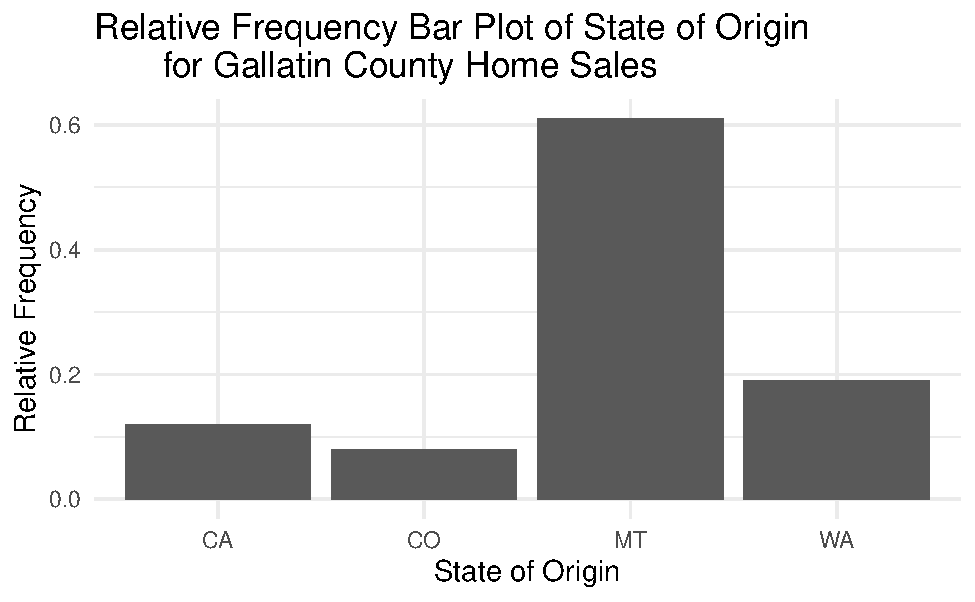
\includegraphics[width=0.65\linewidth]{03-VN03-EDA_OneCatSimulation_files/figure-latex/unnamed-chunk-6-1} \end{center}

\setstretch{1.5}

\begin{itemize}
\tightlist
\item
  Note: the x-axis is the \_\_\_\_\_\_\_\_\_\_\_\_\_\_\_ between the frequency bar plot and the relative frequency bar plot. However, the \_\_\_\_\_\_\_\_\_\_\_\_\_\_ differs. The scale for the frequency bar plot goes from \_\_\_\_\_\_\_\_\_\_\_\_\_\_\_\_\_\_\_\_\_\_\_\_\_\_\_\_\_\_\_ and the scale for the relative frequency bar plot is from \_\_\_\_\_\_\_\_\_\_\_\_\_\_\_\_\_\_\_\_\_\_\_\_\_\_\_\_\_\_.
\end{itemize}

\setstretch{1}

\subsection*{Hypothesis Testing - Video Chapter9}\label{hypothesis-testing---video-chapter9}
\addcontentsline{toc}{subsection}{Hypothesis Testing - Video Chapter9}

Purpose of a hypothesis test:

\begin{itemize}
\item
  Use data collected on a sample to give information about the population.
\item
  Determines \_\_\_\_\_\_\_\_\_\_\_\_\_\_\_\_\_\_ of \_\_\_\_\_\_\_\_\_\_\_\_\_\_\_\_\_\_\_\_\_ of an effect
\end{itemize}

General steps of a hypothesis test

\begin{enumerate}
\def\labelenumi{\arabic{enumi}.}
\item
  Write a research question and hypotheses.
\item
  Collect data and calculate a summary statistic.
\item
  Model a sampling distribution which assumes the null hypothesis is true.
\item
  Calculate a p-value.
\item
  Draw conclusions based on a p-value.
\end{enumerate}

\subsection*{Hypothesis Testing/Justice System}\label{hypothesis-testingjustice-system}
\addcontentsline{toc}{subsection}{Hypothesis Testing/Justice System}

\setstretch{1.5}

\begin{itemize}
\item
  Two possible outcomes if the observed statistic is unusual:

  \begin{itemize}
  \item
    Strong evidence against \_\_\_\_\_\_\_\_\_\_\_\_\_\_\_\_\_\_ -\textgreater{} \_\_\_\_\_\_\_\_\_\_\_\_\_\_\_\_\_\_\_\_
  \item
    Not enough evidence against \_\_\_\_\_\_\_\_\_\_\_\_\_\_\_\_\_\_\_\_\_ -\textgreater{} \_\_\_\_\_\_\_\_\_\_\_\_\_\_\_\_\_\_\_\_\_\_
  \end{itemize}
\item
  Always written about the \_\_\_\_\_\_\_\_\_\_\_\_\_\_\_\_\_\_ (population)
\end{itemize}

\setstretch{1}

\subsubsection*{Null hypothesis}\label{null-hypothesis}
\addcontentsline{toc}{subsubsection}{Null hypothesis}

\begin{itemize}
\item
  Skeptical perspective, no difference, no effect, random chance
\item
  What the researcher hopes is \_\_\_\_\_\_\_\_\_\_\_\_\_\_\_.
\end{itemize}

Notation:

\vspace{0.2in}

\subsubsection*{Alternative hypothesis}\label{alternative-hypothesis}
\addcontentsline{toc}{subsubsection}{Alternative hypothesis}

\begin{itemize}
\item
  New perspective, a chance, a difference, an effect
\item
  What the researcher hopes is \_\_\_\_\_\_\_\_\_\_\_\_\_\_\_\_.
\end{itemize}

Notation:

\vspace{0.2in}

\subsection*{Simulation vs.~Theory-based Methods}\label{simulation-vs.-theory-based-methods}
\addcontentsline{toc}{subsection}{Simulation vs.~Theory-based Methods}

\subsubsection*{Simulation-based method}\label{simulation-based-method}
\addcontentsline{toc}{subsubsection}{Simulation-based method}

\setstretch{1.5}

Creation of the null distribution

\begin{itemize}
\tightlist
\item
  Simulate many samples assuming
\end{itemize}

\vspace{0.2in}

\begin{itemize}
\item
  Find the proportion of \_\_\_\_\_\_\_\_\_\_\_\_\_\_\_\_\_\_\_ at least as extreme as the observed sample \_\_\_\_\_\_\_\_\_\_\_\_
\item
  The null distribution estimates the sample to sample variability expected in the population
\end{itemize}

\setstretch{1}

\subsubsection*{Theory-based method}\label{theory-based-method}
\addcontentsline{toc}{subsubsection}{Theory-based method}

\begin{itemize}
\item
  Use a mathematical model to determine a distribution under the null hypothesis
\item
  Compare the observed sample statistic to the model to calculate a probability
\item
  \emph{Theory-based methods will be discussed in the next module}
\end{itemize}

\subsubsection*{P-value}\label{p-value}
\addcontentsline{toc}{subsubsection}{P-value}

\setstretch{1.5}

\begin{itemize}
\item
  What does the p-value measure?

  \begin{itemize}
  \tightlist
  \item
    Probability of observing the sample \_\_\_\_\_\_\_\_\_\_\_\_\_\_\_\_\_\_\_ or more \_\_\_\_\_\_\_\_\_\_
    assuming the \_\_\_\_\_\_\_\_ hypothesis is \_\_\_\_\_\_\_\_\_\_.
  \end{itemize}
\item
  How much evidence does the p-value provide against the null hypothesis?
\end{itemize}

\begin{center}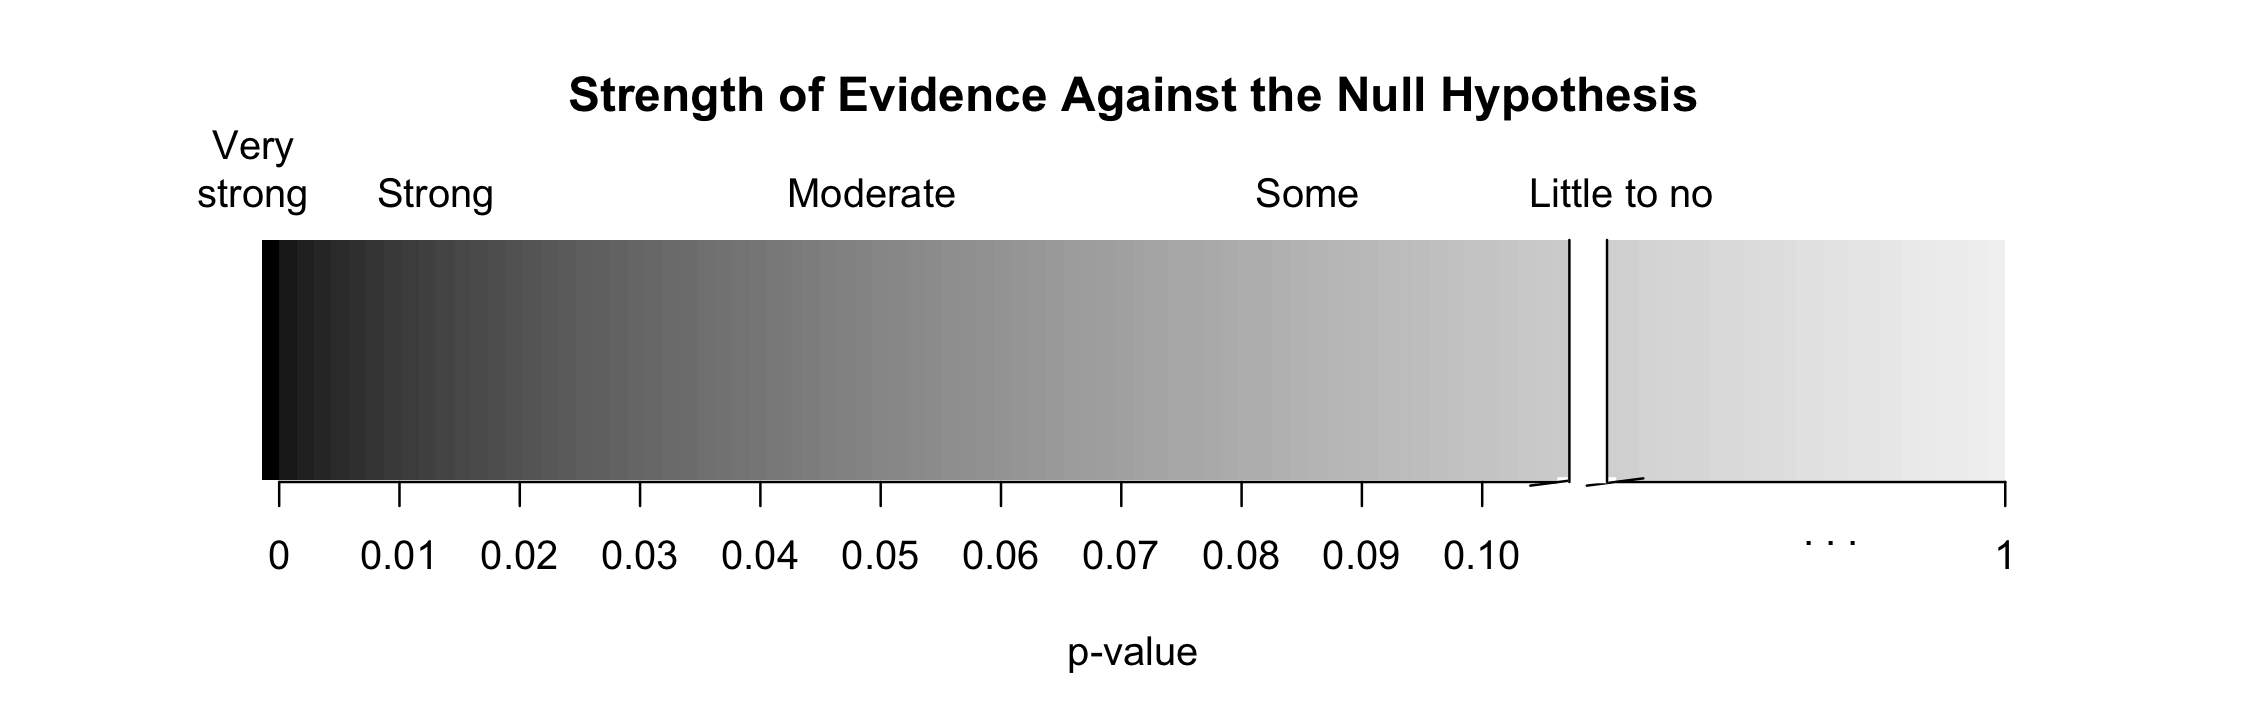
\includegraphics[width=0.75\linewidth]{images/soe_gradient_gray} \end{center}

\rgi \rgi - The \_\_\_\_\_\_\_\_\_\_\_\_\_\_\_\_\_\_the p-value, the \_\_\_\_\_\_\_\_\_\_\_\_\_\_\_\_\_\_\_ the evidence against the null hypothesis.

\begin{itemize}
\tightlist
\item
  Write a conclusion based on the p-value.
\end{itemize}

\rgi \rgi - Answers the \_\_\_\_\_\_\_\_\_\_\_\_\_\_\_\_ question.

\rgi \rgi - Amount of \_\_\_\_\_\_\_\_\_\_\_\_\_\_\_\_\_ in support of the \_\_\_\_\_\_\_\_\_\_\_\_\_\_\_\_\_ hypothesis.

\begin{itemize}
\tightlist
\item
  Decision: can we reject or fail to reject the null hypothesis?
\end{itemize}

\rgi - Significance level: cut-off of ``small'' vs ``large'' p-value

\rgi \rgi - \(\text{p-value} \le \alpha\)

\rgi \rgi \rgi - Strong enough evidence against the null hypothesis

\rgi \rgi \rgi - Decision:

\vspace{0.2in}

\rgi \rgi \rgi - Results are \_\_\_\_\_\_\_\_\_\_\_\_\_\_\_\_\_\_\_\_\_\_\_ significant.

\rgi \rgi - \(\text{p-value} > \alpha\)

\rgi \rgi \rgi - Not enough evidence against the null hypothesis

\rgi \rgi \rgi - Decision:

\vspace{0.17in}

\rgi \rgi \rgi - Results are not \_\_\_\_\_\_\_\_\_\_\_\_\_\_\_\_\_\_\_\_\_ significant.

\setstretch{1}

\subsection*{One proportion test}\label{one-proportion-test}
\addcontentsline{toc}{subsection}{One proportion test}

\begin{itemize}
\item
  Reminder: review summary measures and plots discussed in the Week 3 material and Chapter 4 of the textbook.
\item
  The summary measure for a single categorical variable is a \_\_\_\_\_\_\_\_\_\_\_\_\_\_.
\end{itemize}

Notation:

\begin{itemize}
\item
  Population proportion:
\item
  Sample proportion:
\end{itemize}

Parameter of Interest:

\begin{itemize}
\item
  Include:

  \begin{itemize}
  \item
    Reference of the population (true, long-run, population, all)
  \item
    Summary measure
  \item
    Context

    \begin{itemize}
    \item
      Observational units/cases
    \item
      Response variable (and explanatory variable if present)

      \begin{itemize}
      \tightlist
      \item
        If the response variable is categorical, define a `success' in context
      \end{itemize}
    \end{itemize}
  \end{itemize}
\end{itemize}

\subsubsection*{Hypothesis testing}\label{hypothesis-testing}
\addcontentsline{toc}{subsubsection}{Hypothesis testing}

Conditions:

\begin{itemize}
\tightlist
\item
  Independence:
\end{itemize}

\vspace{0.3in}

Null hypothesis assumes ``no effect'', ``no difference'', ``nothing interesting happening'', etc.

\rgi Always of form: ``parameter'' = null value

\(H_0:\)

\vspace{0.5in}

\(H_A:\)

\vspace{0.5in}

\begin{itemize}
\tightlist
\item
  Research question determines the direction of the alternative hypothesis.
\end{itemize}

Video 14.1 Example: A 2007 study published in the Behavioral Ecology and Sociobiology Journal was titled ``Why do blue-eyed men prefer blue-eyed women?'' (Laeng 2007) In this study, conducted in Norway, 114 volunteer heterosexual blue-eyed males rated the attractiveness of 120 pictures of females. The researchers recorded which eye-color (blue, green, or brown) was rated the highest, on average. In the sample, 51 of the volunteers rated the blue-eyed women the most attractive. Do blue-eyed heterosexual men tend to find blue-eyed women the most attractive?

Parameter of interest:

\vspace{0.5in}

Write the null and alternative hypotheses for the blue-eyed study:

In notation:

\vspace{1mm}

\(H_0:\)

\vspace{0.2in}

\(H_A:\)

\vspace{0.2in}

Statistic:

\vspace{0.4in}

Is the independence condition met to analyze these data using a simulation-based approach?

\vspace{0.2in}

\newpage

\subsubsection*{Simulation-based method}\label{simulation-based-method-1}
\addcontentsline{toc}{subsubsection}{Simulation-based method}

\begin{itemize}
\item
  Simulate many samples assuming \(H_0: \pi = \pi_0\)

  \begin{itemize}
  \item
    Create a spinner with that represents the null value
  \item
    Spin the spinner \(n\) times
  \item
    Calculate and plot the simulated sample proportion from each simulation
  \item
    Repeat 10000 times (simulations) to create the null distribution
  \item
    Find the proportion of simulations at least as extreme as \(\hat{p}\)
  \end{itemize}
\end{itemize}

\begin{Shaded}
\begin{Highlighting}[]
\FunctionTok{set.seed}\NormalTok{(}\DecValTok{216}\NormalTok{)}
\FunctionTok{one\_proportion\_test}\NormalTok{(}\AttributeTok{probability\_success =} \FloatTok{0.333}\NormalTok{, }\CommentTok{\# Null hypothesis value}
          \AttributeTok{sample\_size =} \DecValTok{114}\NormalTok{, }\CommentTok{\# Enter sample size}
          \AttributeTok{number\_repetitions =} \DecValTok{10000}\NormalTok{, }\CommentTok{\# Enter number of simulations}
          \AttributeTok{as\_extreme\_as =} \FloatTok{0.447}\NormalTok{, }\CommentTok{\# Observed statistic}
          \AttributeTok{direction =} \StringTok{"greater"}\NormalTok{, }\CommentTok{\# Specify direction of alternative hypothesis}
          \AttributeTok{summary\_measure =} \StringTok{"proportion"}\NormalTok{) }\CommentTok{\# Reporting proportion or number of successes?}
\end{Highlighting}
\end{Shaded}

\begin{center}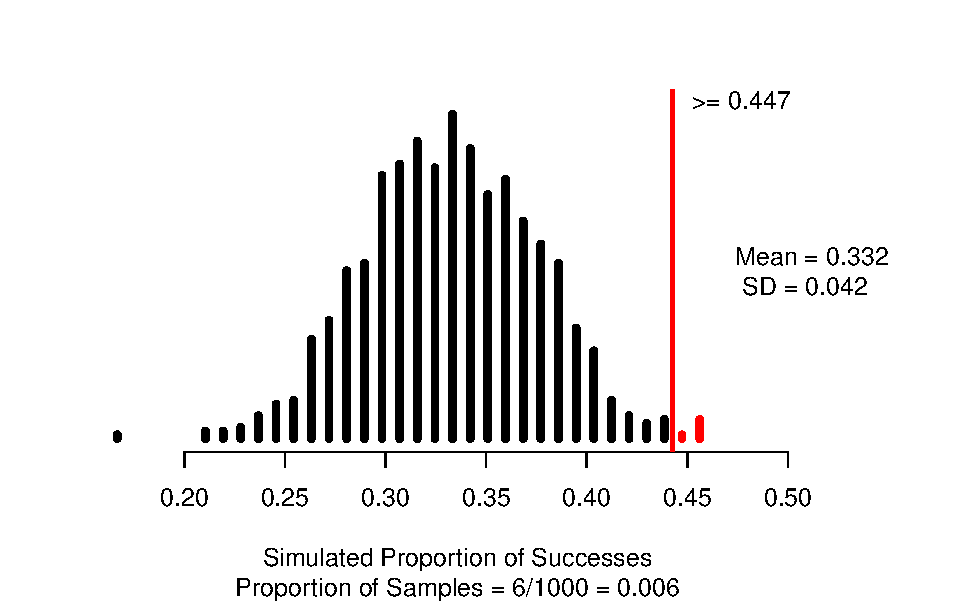
\includegraphics[width=0.7\linewidth]{03-VN03-EDA_OneCatSimulation_files/figure-latex/unnamed-chunk-8-1} \end{center}

Explain why the null distribution is centered at the value of approximately 0.333:

\vspace{0.5in}

Interpretation of the p-value:

\begin{itemize}
\item
  Statement about probability or proportion of samples
\item
  Statistic (summary measure and value)
\item
  Direction of the alternative
\item
  Null hypothesis (in context)
\end{itemize}

\vspace{0.8in}

\newpage

Conclusion:

\begin{itemize}
\item
  Amount of evidence
\item
  Parameter of interest
\item
  Direction of the alternative hypothesis
\end{itemize}

\vspace{0.6in}

Generalization:

\begin{itemize}
\tightlist
\item
  Can the results of the study be generalized to the target population?
\end{itemize}

\vspace{0.4in}

\subsection*{Confidence interval - Video Chapter10}\label{confidence-interval---video-chapter10}
\addcontentsline{toc}{subsection}{Confidence interval - Video Chapter10}

\rgi \(\text{statistic} \pm \text{margin of error}\)

Vocabulary:

\begin{itemize}
\tightlist
\item
  Point estimate:
\end{itemize}

\vspace{0.3in}

\begin{itemize}
\tightlist
\item
  Margin of error:
\end{itemize}

\vspace{0.3in}

\setstretch{1.5}

Purpose of a confidence interval

\begin{itemize}
\item
  To give an \_\_\_\_\_\_\_\_\_\_\_\_\_\_\_\_\_\_\_\_ \_\_\_\_\_\_\_\_\_\_\_\_\_\_\_\_\_\_\_ for the parameter of interest
\item
  Determines how \_\_\_\_\_\_\_\_\_\_\_\_\_\_ an effect is
\end{itemize}

\setstretch{1}

\subsubsection*{Sampling distribution}\label{sampling-distribution}
\addcontentsline{toc}{subsubsection}{Sampling distribution}

\setstretch{1.5}

\begin{itemize}
\item
  Ideally, we would take many samples of the same \_\_\_\_\_\_\_\_\_\_\_ from the same population to create a sampling distribution
\item
  But only have 1 sample, so we will \_\_\_\_\_\_\_\_\_\_\_\_\_\_\_\_\_ with \_\_\_\_\_\_\_\_\_\_\_\_\_\_\_\_\_ from the one sample.
\item
  Need to estimate the sampling distribution to see the \_\_\_\_\_\_\_\_\_\_\_\_\_\_\_\_\_ in the sample
\end{itemize}

\setstretch{1}

\subsubsection*{Simulation-based methods}\label{simulation-based-methods}
\addcontentsline{toc}{subsubsection}{Simulation-based methods}

Bootstrap distribution:

\begin{itemize}
\item
  Write the response variable values on cards
\item
  Sample with replacement \(n\) times (bootstrapping)
\item
  Calculate and plot the simulated difference in sample means from each simulation
\item
  Repeat 10000 times (simulations) to create the bootstrap distribution
\item
  Find the cut-offs for the middle X\% (confidence level) in a bootstrap distribution.
\end{itemize}

What is bootstrapping?

\begin{itemize}
\item
  Assume the ``population'' is many, many copies of the original sample.
\item
  Randomly sample with replacement from the original sample \(n\) times.
\end{itemize}

\subsubsection*{Video 14.2}\label{video-14.2}
\addcontentsline{toc}{subsubsection}{Video 14.2}

Let's revisit the blue-eyed male study to estimate the \emph{proportion of ALL heterosexual blue-eyed males who tend to find blue-eyed women the most attractive} by creating a 90\% confidence interval.

Bootstrap distribution:

\begin{Shaded}
\begin{Highlighting}[]
\FunctionTok{set.seed}\NormalTok{(}\DecValTok{216}\NormalTok{)}
\FunctionTok{one\_proportion\_bootstrap\_CI}\NormalTok{(}\AttributeTok{sample\_size =} \DecValTok{114}\NormalTok{, }\CommentTok{\# Sample size}
                    \AttributeTok{number\_successes =} \DecValTok{51}\NormalTok{, }\CommentTok{\# Observed number of successes}
                    \AttributeTok{number\_repetitions =} \DecValTok{10000}\NormalTok{, }\CommentTok{\# Number of bootstrap samples to use}
                    \AttributeTok{confidence\_level =} \FloatTok{0.90}\NormalTok{) }\CommentTok{\# Confidence level as a decimal}
\end{Highlighting}
\end{Shaded}

\begin{center}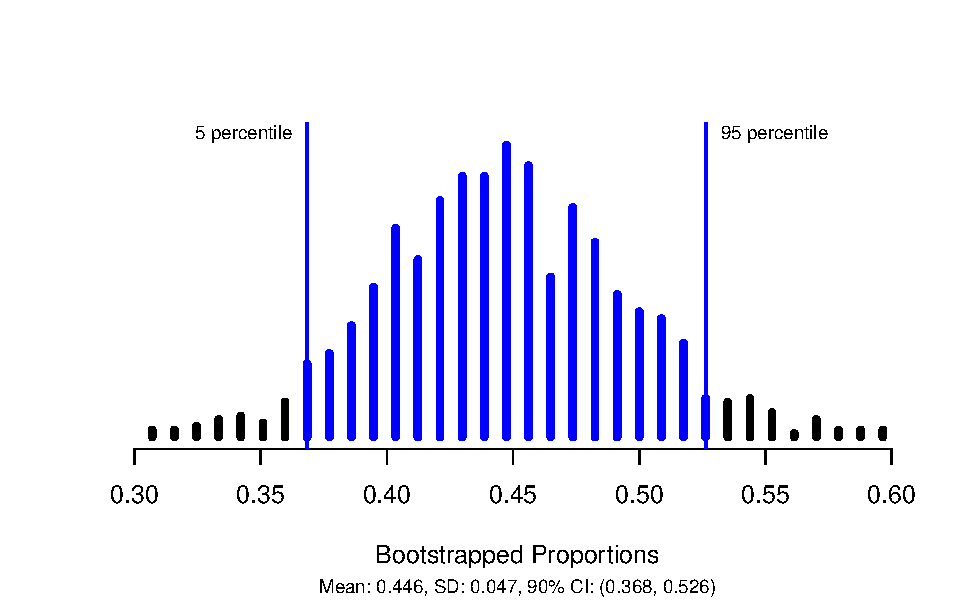
\includegraphics[width=0.7\linewidth]{03-VN03-EDA_OneCatSimulation_files/figure-latex/unnamed-chunk-9-1} \end{center}

Confidence interval interpretation:

\begin{itemize}
\item
  How confident you are (e.g., 90\%, 95\%, 98\%, 99\%)
\item
  Parameter of interest
\item
  Calculated interval
\item
  Order of subtraction when comparing two groups
\end{itemize}

\vspace{0.8in}

\newpage

How does changing the confidence level impact the width of the confidence interval?

95\% Confidence Interval:

\begin{Shaded}
\begin{Highlighting}[]
\FunctionTok{set.seed}\NormalTok{(}\DecValTok{216}\NormalTok{)}
\FunctionTok{one\_proportion\_bootstrap\_CI}\NormalTok{(}\AttributeTok{sample\_size =} \DecValTok{114}\NormalTok{, }\CommentTok{\# Sample size}
                    \AttributeTok{number\_successes =} \DecValTok{51}\NormalTok{, }\CommentTok{\# Observed number of successes}
                    \AttributeTok{number\_repetitions =} \DecValTok{10000}\NormalTok{, }\CommentTok{\# Number of bootstrap samples to use}
                    \AttributeTok{confidence\_level =} \FloatTok{0.95}\NormalTok{) }\CommentTok{\# Confidence level as a decimal}
\end{Highlighting}
\end{Shaded}

\begin{center}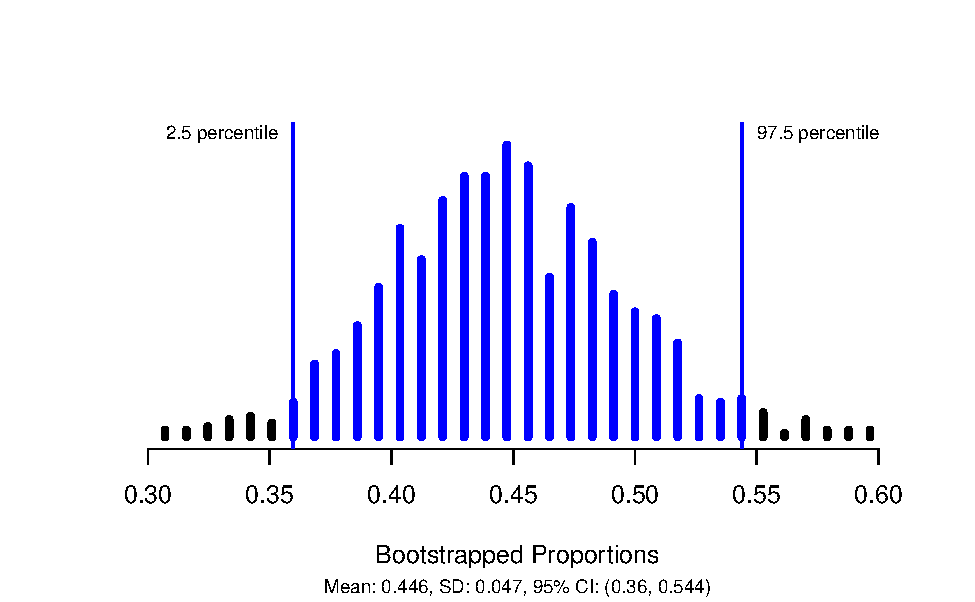
\includegraphics[width=0.7\linewidth]{03-VN03-EDA_OneCatSimulation_files/figure-latex/unnamed-chunk-10-1} \end{center}

99\% Confidence Interval:

\begin{Shaded}
\begin{Highlighting}[]
\FunctionTok{set.seed}\NormalTok{(}\DecValTok{216}\NormalTok{)}
\FunctionTok{one\_proportion\_bootstrap\_CI}\NormalTok{(}\AttributeTok{sample\_size =} \DecValTok{114}\NormalTok{, }\CommentTok{\# Sample size}
                    \AttributeTok{number\_successes =} \DecValTok{51}\NormalTok{, }\CommentTok{\# Observed number of successes}
                    \AttributeTok{number\_repetitions =} \DecValTok{10000}\NormalTok{, }\CommentTok{\# Number of bootstrap samples to use}
                    \AttributeTok{confidence\_level =} \FloatTok{0.99}\NormalTok{) }\CommentTok{\# Confidence level as a decimal}
\end{Highlighting}
\end{Shaded}

\begin{center}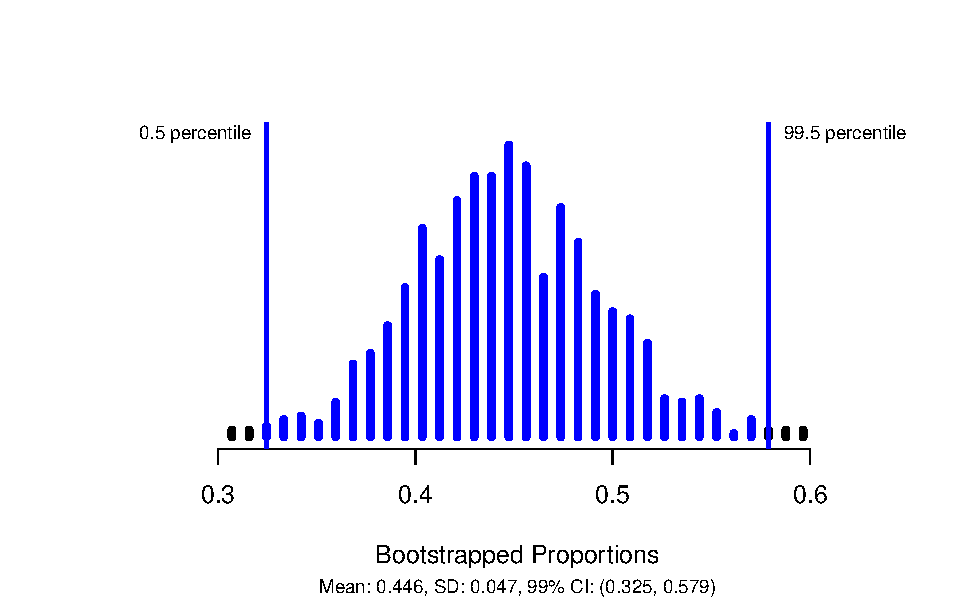
\includegraphics[width=0.7\linewidth]{03-VN03-EDA_OneCatSimulation_files/figure-latex/unnamed-chunk-11-1} \end{center}

\subsection{Concept Check}\label{concept-check-3}

Be prepared for group discussion in the next class. One member from the table should write the answers to the following on the whiteboard.

\begin{enumerate}
\def\labelenumi{\arabic{enumi}.}
\tightlist
\item
  What is the summary measure calculated from a single categorical variable?
\end{enumerate}

\vspace{0.3in}

\begin{enumerate}
\def\labelenumi{\arabic{enumi}.}
\setcounter{enumi}{1}
\tightlist
\item
  Write the alternative hypothesis for this study in notation? How was the direction of the alternative hypothesis determined?
\end{enumerate}

\vspace{0.4in}

\begin{enumerate}
\def\labelenumi{\arabic{enumi}.}
\setcounter{enumi}{2}
\tightlist
\item
  Do the results of the confidence interval \emph{match} the results based on the p-value?
\end{enumerate}

\vspace{0.5in}

\newpage

\section{Activity 6: Helper-Hinderer Part 1 --- Simulation-based Hypothesis Test}\label{activity-6-helper-hinderer-part-1-simulation-based-hypothesis-test}

\setstretch{1}

\subsection{Learning outcomes}\label{learning-outcomes-5}

\begin{itemize}
\item
  Identify the two possible explanations (one assuming the null hypothesis and one assuming the alternative hypothesis) for a relationship seen in sample data.
\item
  Given a research question involving a single categorical variable, construct the null and alternative hypotheses
  in words and using appropriate statistical symbols.
\item
  Describe and perform a simulation-based hypothesis test for a single proportion.
\end{itemize}

\subsection{Terminology review}\label{terminology-review-5}

In today's activity, we will work through a simulation-based hypothesis testing for a single categorical variable. Some terms covered in this activity are:

\begin{itemize}
\item
  Parameter of interest
\item
  Null hypothesis
\item
  Alternative hypothesis
\item
  Simulation
\end{itemize}

To review these concepts, see Chapters 9 \& 14 in your textbook.

\subsection{Steps of the statistical investigation process}\label{steps-of-the-statistical-investigation-process-2}

We will work through a five-step process to complete a hypothesis test for a single proportion, first introduced in the activity in week 1.

\begin{itemize}
\item
  \textbf{Ask a research question} that can be addressed by collecting data. What are the researchers trying to show?
\item
  \textbf{Design a study and collect data}. This step involves selecting the people or objects to be studied and how to gather relevant data on them.
\item
  \textbf{Summarize and visualize the data}. Calculate summary statistics and create graphical plots that best represent the research question.
\item
  \textbf{Use statistical analysis methods to draw inferences from the data}. Choose a statistical inference method appropriate for the data and identify the p-value and/or confidence interval after checking assumptions. In this study, we will focus on using randomization to generate a simulated p-value.
\item
  \textbf{Communicate the results and answer the research question}. Using the p-value and confidence interval from the analysis, determine whether the data provide statistical evidence against the null hypothesis. Write a conclusion that addresses the research question.
\end{itemize}

\newpage

\subsection{Helper-Hinderer}\label{helper-hinderer}

A study by Hamblin, Wynn, and Bloom reported in Nature (Hamblin, Wynn, and Bloom 2007) was intended to check young kids' feelings about helpful and non-helpful behavior. Non-verbal infants ages 6 to 10 months were shown short videos with different shapes either helping or hindering the climber. As a class we will watch this short video to see how the experiment was run: \url{https://youtu.be/anCaGBsBOxM}. Researchers were hoping to assess: Are infants more likely to choose the helper toy over the hinderer toy? In the study, of the 16 infants age 6 to 10 months, 14 chose the \emph{helper} toy and 2 chose the \emph{hinderer} toy.

In this study, the \textbf{observational units are the infants ages 6 to 10 months}. The \textbf{variable measured on each observational unit (infant) is whether they chose the helper or the hinderer toy}. This is a categorical variable so we will be assessing the proportion of infants ages 6 to 10 months that choose the helper toy. Choosing the helper toy in this study will be considered a success.

\subsubsection*{Ask a research question}\label{ask-a-research-question}
\addcontentsline{toc}{subsubsection}{Ask a research question}

\begin{enumerate}
\def\labelenumi{\arabic{enumi}.}
\tightlist
\item
  Identify the research question for this study. What are the researchers hoping to show?
\end{enumerate}

\vspace{0.6in}

\subsubsection*{Design a study and collect data}\label{design-a-study-and-collect-data}
\addcontentsline{toc}{subsubsection}{Design a study and collect data}

Before using statistical inference methods, we must check that the cases are independent. The sample observations are independent if the outcome of one observation does not influence the outcome of another. One way this condition is met is if data come from a simple random sample of the target population.

\begin{enumerate}
\def\labelenumi{\arabic{enumi}.}
\setcounter{enumi}{1}
\tightlist
\item
  Are the cases independent? Justify your answer.
\end{enumerate}

\vspace{0.8in}

\subsubsection*{R code}\label{r-code}
\addcontentsline{toc}{subsubsection}{R code}

For almost all activities and labs it will be necessary to upload the provided R script file from D2L for that day. Your instructor will highlight a few steps in uploading files to and using RStudio.

The following are the steps to upload the necessary R script file for this activity:

\begin{itemize}
\item
  Download the Activity R script file from D2L.
\item
  Click ``Upload'' in the ``Files'' tab in the bottom right window of RStudio. In the pop-up window, click ``Choose File'', and navigate to the folder where the Activity R script file is saved (most likely in your downloads folder). Click ``Open''; then click ``Ok''.
\item
  You should see the uploaded file appear in the list of files in the bottom right window. Click on the file name to open the file in the Editor window (upper left window).
\end{itemize}

Notice that the first threelines of code contain a prompt called \texttt{library}. Packages needed to run functions in R are stored in directories called libraries. When using the MSU RStudio server, all the packages needed for the class are already installed. We simply must tell R which packages we need for each R script file. We use the prompt \texttt{library} to load each \textbf{package} (or library) needed for each activity. Note, these \texttt{library} lines MUST be run each time you open a R script file in order for the functions in R to work.

\begin{itemize}
\tightlist
\item
  Highlight and run lines 1--3 to load the packages needed for this activity. Notice the use of the \# symbol in the R script file. This symbol is not part of the R code. It is used by these authors to add comments to the R code and explain what each call is telling the program to do.
\end{itemize}

R will ignore everything after a \# symbol when executing the code. Refer to the instructions following the \# symbol to understand what you need to enter in the code.

\begin{Shaded}
\begin{Highlighting}[]
\FunctionTok{library}\NormalTok{(tidyverse)}
\FunctionTok{library}\NormalTok{(ggplot2)}
\FunctionTok{library}\NormalTok{(catstats)}
\end{Highlighting}
\end{Shaded}

Throughout activities, we will often include the R code you would use in order to produce output or plots. These ``code chunks'' appear in gray. In the code chunk below, we demonstrate how to read the data set into R using the \texttt{read.csv()} function. The line of code shown below (line 7 in the R script file) reads in the data set and names the data set \texttt{infants}.

\subsubsection*{Summarize and visualize the data}\label{summarize-and-visualize-the-data}
\addcontentsline{toc}{subsubsection}{Summarize and visualize the data}

The following code reads in the data set and gives the number of infants in each level of the variable, whether the infant chose the helper or the hinderer.

\begin{itemize}
\tightlist
\item
  Highlight and run lines 7 and 8 to check that you get the same counts as shown below
\end{itemize}

\begin{Shaded}
\begin{Highlighting}[]
 \CommentTok{\# Read in data set}
\NormalTok{infants }\OtherTok{\textless{}{-}} \FunctionTok{read.csv}\NormalTok{(}\StringTok{"https://math.montana.edu/courses/s216/data/infantchoice.csv"}\NormalTok{)}
\NormalTok{infants }\SpecialCharTok{\%\textgreater{}\%} \FunctionTok{count}\NormalTok{(choice)  }\CommentTok{\# Count number in each choice category}
\end{Highlighting}
\end{Shaded}

\begin{verbatim}
#>     choice  n
#> 1   helper 14
#> 2 hinderer  2
\end{verbatim}

The following formula is used to calculate the proportion of successes in the sample.

\[\hat{p} = \frac{\mbox{number of successes}}{\mbox{total number of observational units}}\]

\begin{enumerate}
\def\labelenumi{\arabic{enumi}.}
\setcounter{enumi}{2}
\tightlist
\item
  Using the R output and the formula given, calculate the summary statistic (sample proportion) to represent the research question. Recall that \texttt{choosing\ the\ helper\ toy} is a considered a success. Use appropriate notation.
\end{enumerate}

\vspace{0.5in}

To visually display this data we can use either a frequency bar plot or a relative frequency bar plot.

\begin{itemize}
\item
  Enter the variable name \texttt{choice} for \texttt{variable} in the R code to create the frequency bar plot.
\item
  Note the name of the title is given in line 16 and includes the type of plot, observational units, and variable name
\item
  Highlight and run lines 13--19 to create the plot
\end{itemize}

\begin{Shaded}
\begin{Highlighting}[]
\NormalTok{infants }\SpecialCharTok{\%\textgreater{}\%} \CommentTok{\# Data set piped into...}
    \FunctionTok{ggplot}\NormalTok{(}\FunctionTok{aes}\NormalTok{(}\AttributeTok{x =}\NormalTok{ variable)) }\SpecialCharTok{+}   \CommentTok{\# This specifies the variable}
    \FunctionTok{geom\_bar}\NormalTok{(}\AttributeTok{stat =} \StringTok{"count"}\NormalTok{) }\SpecialCharTok{+}  \CommentTok{\# Tell it to make a bar plot}
    \FunctionTok{labs}\NormalTok{(}\AttributeTok{title =} \StringTok{"Frequency Bar Plot of Toy Choice for Pre{-}verbal Infants"}\NormalTok{,  }
       \CommentTok{\# Give your plot a title}
       \AttributeTok{x =} \StringTok{"Toy Choice"}\NormalTok{,   }\CommentTok{\# Label the x axis}
       \AttributeTok{y =} \StringTok{"Frequency"}\NormalTok{)  }\CommentTok{\# Label the y axis}
\end{Highlighting}
\end{Shaded}

\begin{enumerate}
\def\labelenumi{\arabic{enumi}.}
\setcounter{enumi}{3}
\tightlist
\item
  Sketch the frequency bar plot created below.
\end{enumerate}

\vspace{1.8in}

We could also choose to display the data as a proportion in a \textbf{relative frequency} bar plot. To find the relative frequency, the count in each level of \texttt{choice} is divided by the sample size. This calculation is the sample proportion for each level of \texttt{choice}. Notice that in the following code we told R to create a bar plot with proportions.

\begin{itemize}
\tightlist
\item
  In the R script file, highlight and run lines 23--29 to create the relative frequency bar plot.
\end{itemize}

\begin{Shaded}
\begin{Highlighting}[]
\NormalTok{infants }\SpecialCharTok{\%\textgreater{}\%} \CommentTok{\# Data set piped into...}
    \FunctionTok{ggplot}\NormalTok{(}\FunctionTok{aes}\NormalTok{(}\AttributeTok{x =}\NormalTok{ choice)) }\SpecialCharTok{+}   \CommentTok{\# This specifies the variable}
    \FunctionTok{geom\_bar}\NormalTok{(}\FunctionTok{aes}\NormalTok{(}\AttributeTok{y =} \FunctionTok{after\_stat}\NormalTok{(prop), }\AttributeTok{group =} \DecValTok{1}\NormalTok{)) }\SpecialCharTok{+}  \CommentTok{\# Tell it to make a bar plot with proportions}
    \FunctionTok{labs}\NormalTok{(}\AttributeTok{title =} \StringTok{"Relative Frequency Bar Plot of Toy Choice for Pre{-}verbal Infants"}\NormalTok{,  }
       \CommentTok{\# Give your plot a title}
       \AttributeTok{x =} \StringTok{"Toy Choice"}\NormalTok{,   }\CommentTok{\# Label the x axis}
       \AttributeTok{y =} \StringTok{"Relative Frequency"}\NormalTok{)  }\CommentTok{\# Label the y axis}
\end{Highlighting}
\end{Shaded}

\begin{center}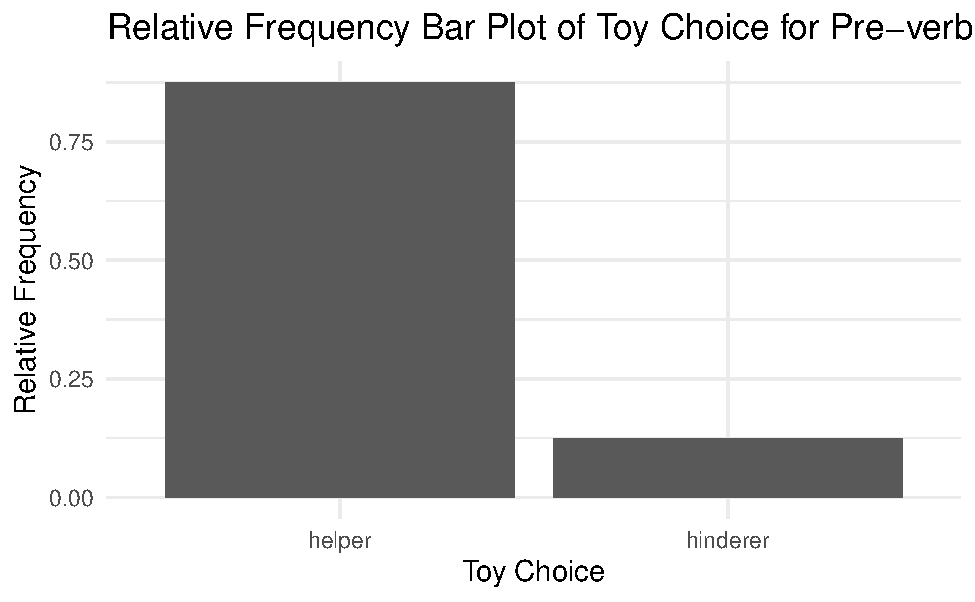
\includegraphics[width=0.5\linewidth]{03-A06-inference-1cat_test-simulation_files/figure-latex/unnamed-chunk-4-1} \end{center}

\begin{enumerate}
\def\labelenumi{\arabic{enumi}.}
\setcounter{enumi}{4}
\tightlist
\item
  Which features in the relative frequency bar plot are the same as the frequency bar plot? Which are different?
\end{enumerate}

\vspace{0.5in}

We cannot assess whether infants are more likely to choose the helper toy based on the statistic and plot alone. The next step is to analyze the data by using a hypothesis test to discover if there is evidence against the null hypothesis.

\subsubsection*{Use statistical analysis methods to draw inferences from the data}\label{use-statistical-analysis-methods-to-draw-inferences-from-the-data}
\addcontentsline{toc}{subsubsection}{Use statistical analysis methods to draw inferences from the data}

When performing a hypothesis test, we must first identify the null hypothesis. The null hypothesis is written about the parameter of interest, or the value that summarizes the variable in the population.

The parameter of interest is a statement about what we want to find about the population. The following must be included when writing the parameter of interest.

\begin{itemize}
\item
  Population word (true, long-run, population)
\item
  Summary measure (depends on the type of data)
\item
  Context

  \begin{itemize}
  \item
    Observational units
  \item
    Variable(s)
  \end{itemize}
\end{itemize}

For this study, the parameter of interest, \(\pi\), represents the \textbf{true or population proportion of infants ages 6--10 months who will choose the helper toy}.

If the children are just randomly choosing the toy, we would expect half (0.5) of the infants to choose the helper toy. This is the null value for our study.

\begin{enumerate}
\def\labelenumi{\arabic{enumi}.}
\setcounter{enumi}{5}
\tightlist
\item
  Using the parameter of interest given above, write out the null hypothesis in words. That is, what do we assume to be true about the parameter of interest when we perform our simulation?
  \vspace{0.8in}
\end{enumerate}

The notation used for a population proportion (or probability, or true proportion) is \(\pi\). Since this summarizes a population, it is a parameter. When writing the \textbf{null hypothesis} in notation, we set the parameter equal to the null value, \(H_0: \pi = \pi_0\).

\begin{enumerate}
\def\labelenumi{\arabic{enumi}.}
\setcounter{enumi}{6}
\tightlist
\item
  Write the null hypothesis in notation using the null value of 0.5 in place of \(\pi_0\) in the equation given above.
\end{enumerate}

\vspace{0.5in}

The \textbf{alternative hypothesis} is the claim to be tested and the direction of the claim (less than, greater than, or not equal to) is based on the research question.

\begin{enumerate}
\def\labelenumi{\arabic{enumi}.}
\setcounter{enumi}{7}
\tightlist
\item
  Based on the research question from question 1, are we testing that the parameter is greater than 0.5, less than 0.5 or different than 0.5?
\end{enumerate}

\vspace{0.2in}

\begin{enumerate}
\def\labelenumi{\arabic{enumi}.}
\setcounter{enumi}{8}
\tightlist
\item
  Write out the alternative hypothesis in notation.
\end{enumerate}

\vspace{0.5in}

Remember that when utilizing a hypothesis test, we are evaluating two competing possibilities. For this study the \textbf{two possibilities} are either\ldots{}

\begin{itemize}
\item
  The true proportion of infants who choose the helper is 0.5 and our results just occurred by random chance; or,
\item
  The true proportion of infants who choose the helper is greater than 0.5 and our results reflect this.
\end{itemize}

Notice that these two competing possibilities represent the null and alternative hypotheses.

We will now simulate one sample of a \textbf{null distribution} of sample proportions. The null distribution is created under the assumption the null hypothesis is true. In this case, we assume the true proportion of infants who choose the helper is 0.5, so we will create 10000 (or more) different simulations of 16 infants under this assumption.

Let's think about how to use a coin to create one simulation of 16 infants under the assumption the null hypothesis is true. Let heads equal infant chose the helper toy and tails equal infant chose the hinderer toy.

\begin{enumerate}
\def\labelenumi{\arabic{enumi}.}
\setcounter{enumi}{9}
\tightlist
\item
  How many times would you flip a coin to simulate the sample of infants?
\end{enumerate}

\vspace{0.2in}

\begin{enumerate}
\def\labelenumi{\arabic{enumi}.}
\setcounter{enumi}{10}
\tightlist
\item
  Flip a coin 16 times recording the number of times the coin lands on heads. This represents one simulated sample of 16 infants randomly choosing the toy. Calculate the proportion of coin flips that resulted in heads.
\end{enumerate}

\vspace{0.2in}

\begin{enumerate}
\def\labelenumi{\arabic{enumi}.}
\setcounter{enumi}{11}
\tightlist
\item
  Is the value from question 11 closer to 0.5, the null value, or closer to the sample proportion, 0.875?
\end{enumerate}

\vspace{0.2in}

Report the number of coin flips you got as indicated by your instructor.

\begin{enumerate}
\def\labelenumi{\arabic{enumi}.}
\setcounter{enumi}{12}
\tightlist
\item
  Sketch the graph created by your instructor of the proportion of heads out of 16 coin flips.
\end{enumerate}

\vspace{2in}

\begin{enumerate}
\def\labelenumi{\arabic{enumi}.}
\setcounter{enumi}{13}
\tightlist
\item
  Circle the observed statistic (value from question 3) on the distribution shown above. Where does this statistic fall in this distribution: Is it near the center of the distribution (near 0.5) or in one of the tails of the distribution?
\end{enumerate}

\vspace{0.2in}

\begin{enumerate}
\def\labelenumi{\arabic{enumi}.}
\setcounter{enumi}{14}
\tightlist
\item
  Is the observed statistic likely to happen or unlikely to happen if the true proportion of infants who choose the helper is 0.5? Explain your answer using the plot.
\end{enumerate}

\vspace{0.8in}

In the next class, we will continue to assess the strength of evidence against the null hypothesis by using a computer to simulate 10000 samples when we assume the null hypothesis is true.

\newpage

\subsection{Take-home messages}\label{take-home-messages-5}

\begin{enumerate}
\def\labelenumi{\arabic{enumi}.}
\item
  Two types of plots are used for plotting categorical variables: frequency bar plots, relative frequency bar plots.
\item
  In a hypothesis test we have two competing hypotheses, the null hypothesis and the alternative hypothesis. The null hypothesis represents either a skeptical perspective or a perspective of no difference or no effect. The alternative hypothesis represents a new perspective such as the possibility that there has been a change or that there is a treatment effect in an experiment.
\item
  In a simulation-based test, we create a distribution of possible simulated statistics for our sample if the null hypothesis is true. Then we see if the calculated observed statistic from the data is likely or unlikely to occur when compared to the null distribution.
\item
  To create one simulated sample on the null distribution for a sample proportion, spin a spinner with probability equal to \(\pi_0\) (the null value), \(n\) times or draw with replacement \(n\) times from a deck of cards created to reflect \(\pi_0\) as the probability of success. Calculate and plot the proportion of successes from the simulated sample.
\end{enumerate}

\subsection{Additional notes}\label{additional-notes-5}

Use this space to summarize your thoughts and take additional notes on today's activity and material covered.

\newpage

\section{Activity 7: Helper-Hinderer (continued)}\label{activity-7-helper-hinderer-continued}

\setstretch{1}

\subsection{Learning outcomes}\label{learning-outcomes-6}

\begin{itemize}
\item
  Describe and perform a simulation-based hypothesis test for a single proportion.
\item
  Interpret and evaluate a p-value for a simulation-based hypothesis test for a single proportion.
\item
  Explore what a p-value represents
\end{itemize}

\subsection{Steps of the statistical investigation process}\label{steps-of-the-statistical-investigation-process-3}

In today's activity we will continue with steps 4 and 5 in the statistical investigation process. We will continue to assess the Helper-Hinderer study from last class.

\begin{itemize}
\item
  \textbf{Ask a research question} that can be addressed by collecting data. What are the researchers trying to show?
\item
  \textbf{Design a study and collect data}. This step involves selecting the people or objects to be studied and how to gather relevant data on them.
\item
  \textbf{Summarize and visualize the data}. Calculate summary statistics and create graphical plots that best represent the research question.
\item
  \textbf{Use statistical analysis methods to draw inferences from the data}. Choose a statistical inference method appropriate for the data and identify the p-value and/or confidence interval after checking assumptions. In this study, we will focus on using randomization to generate a simulated p-value.
\item
  \textbf{Communicate the results and answer the research question}. Using the p-value and confidence interval from the analysis, determine whether the data provide statistical evidence against the null hypothesis. Write a conclusion that addresses the research question.
\end{itemize}

\subsection{Helper-Hinderer}\label{helper-hinderer-1}

In class today, we will revisit the study on infants as described below.

A study by Hamblin, Wynn, and Bloom reported in Nature (Hamblin, Wynn, and Bloom 2007) was intended to check young kids' feelings about helpful and non-helpful behavior. Non-verbal infants ages 6 to 10 months were shown short videos with different shapes either helping or hindering the climber. As a class we will watch this short video to see how the experiment was run: \url{https://youtu.be/anCaGBsBOxM}. Researchers were hoping to assess: Are infants more likely to choose the helper toy over the hinderer toy? In the study, of the 16 infants age 6 to 10 months, 14 chose the \emph{helper} toy and 2 chose the \emph{hinderer} toy.

\begin{enumerate}
\def\labelenumi{\arabic{enumi}.}
\tightlist
\item
  Report the sample proportion (summary statistic) calculated in the previous activity.
\end{enumerate}

\vspace{0.3in}

\begin{enumerate}
\def\labelenumi{\arabic{enumi}.}
\setcounter{enumi}{1}
\tightlist
\item
  Write the alternative hypothesis in words in context of the problem. Remember the direction we are testing is dependent on the research question.
\end{enumerate}

\vspace{0.8in}

Today, we will use the computer to simulate a null distribution of 10000 different samples of 16 infants, plotting the proportion who chose the helper in each sample, based on the assumption that the true proportion of infants who choose the helper is 0.5 (or that the null hypothesis is true).

\newpage

To use the computer simulation, we will need to enter the

\begin{itemize}
\tightlist
\item
  assumed ``probability of success'' (\(\pi_0\)),
\item
  ``sample size'' (the number of observational units or cases in the sample),
\item
  ``number of repetitions'' (the number of samples to be generated - typically we use 10000),
\item
  ``as extreme as'' (the observed statistic), and
\item
  the ``direction'' (matches the direction of the alternative hypothesis).
\end{itemize}

\begin{enumerate}
\def\labelenumi{\arabic{enumi}.}
\setcounter{enumi}{2}
\tightlist
\item
  What values should be entered for each of the following into the one proportion test to create 10000 simulations?
\end{enumerate}

\vspace{1mm}

\begin{itemize}
\tightlist
\item
  Probability of success:
\end{itemize}

\vspace{.2in}

\begin{itemize}
\tightlist
\item
  Sample size:
\end{itemize}

\vspace{.2in}

\begin{itemize}
\tightlist
\item
  Number of repetitions:
\end{itemize}

\vspace{.2in}

\begin{itemize}
\tightlist
\item
  As extreme as:
\end{itemize}

\vspace{.2in}

\begin{itemize}
\tightlist
\item
  Direction (\texttt{"greater"}, \texttt{"less"}, or \texttt{"two-sided"}):
\end{itemize}

We will use the \texttt{one\_proportion\_test()} function in \texttt{R} (in the \texttt{catstats} package) to simulate the null distribution of sample proportions and compute a p-value. Using the provided \texttt{R} script file, fill in the values/words for each \texttt{xx} with your answers from question 3 in the one proportion test to create a null distribution with 10000 simulations. Then highlight and run lines 1--16.

\begin{Shaded}
\begin{Highlighting}[]
\FunctionTok{one\_proportion\_test}\NormalTok{(}\AttributeTok{probability\_success =}\NormalTok{ xx, }\CommentTok{\# Null hypothesis value}
          \AttributeTok{sample\_size =}\NormalTok{ xx, }\CommentTok{\# Enter sample size}
          \AttributeTok{number\_repetitions =} \DecValTok{10000}\NormalTok{, }\CommentTok{\# Enter number of simulations}
          \AttributeTok{as\_extreme\_as =}\NormalTok{ xx, }\CommentTok{\# Observed statistic}
          \AttributeTok{direction =} \StringTok{"xx"}\NormalTok{, }\CommentTok{\# Specify direction of alternative hypothesis}
          \AttributeTok{summary\_measure =} \StringTok{"proportion"}\NormalTok{) }\CommentTok{\# Reporting proportion or number of successes?}
\end{Highlighting}
\end{Shaded}

\begin{enumerate}
\def\labelenumi{\arabic{enumi}.}
\setcounter{enumi}{3}
\tightlist
\item
  Sketch the null distribution created from the \texttt{R} code here.
\end{enumerate}

\vspace{1.8in}

\begin{enumerate}
\def\labelenumi{\arabic{enumi}.}
\setcounter{enumi}{4}
\tightlist
\item
  Around what value is the null distribution centered? Why does that make sense?
\end{enumerate}

\vspace{1in}

\begin{enumerate}
\def\labelenumi{\arabic{enumi}.}
\setcounter{enumi}{5}
\tightlist
\item
  Circle the observed statistic (value from question 1) on the distribution you drew in question 4. Where does this statistic fall in the null distribution: Is it near the center of the distribution (near 0.5) or in one of the tails of the distribution?
\end{enumerate}

\vspace{0.2in}

\begin{enumerate}
\def\labelenumi{\arabic{enumi}.}
\setcounter{enumi}{6}
\tightlist
\item
  Is the observed statistic likely to happen or unlikely to happen if the true proportion of infants who choose the helper is 0.5? Explain your answer using the plot.
\end{enumerate}

\vspace{0.5in}

\begin{enumerate}
\def\labelenumi{\arabic{enumi}.}
\setcounter{enumi}{7}
\tightlist
\item
  Using the simulation, what is the proportion of simulated samples that generated a sample proportion at the observed statistic or greater, if the true proportion of infants who choose the helper is 0.5? \emph{Hint}: Look under the simulation.
\end{enumerate}

\vspace{0.2in}

The value in question 8 is the \textbf{p-value}. The smaller the p-value, the more evidence we have against the null hypothesis.

\begin{enumerate}
\def\labelenumi{\arabic{enumi}.}
\setcounter{enumi}{8}
\tightlist
\item
  Using the following guidelines for the strength of evidence, how much evidence do the data provide against the null hypothesis? (Circle one of the five descriptions.)
\end{enumerate}

\begin{center}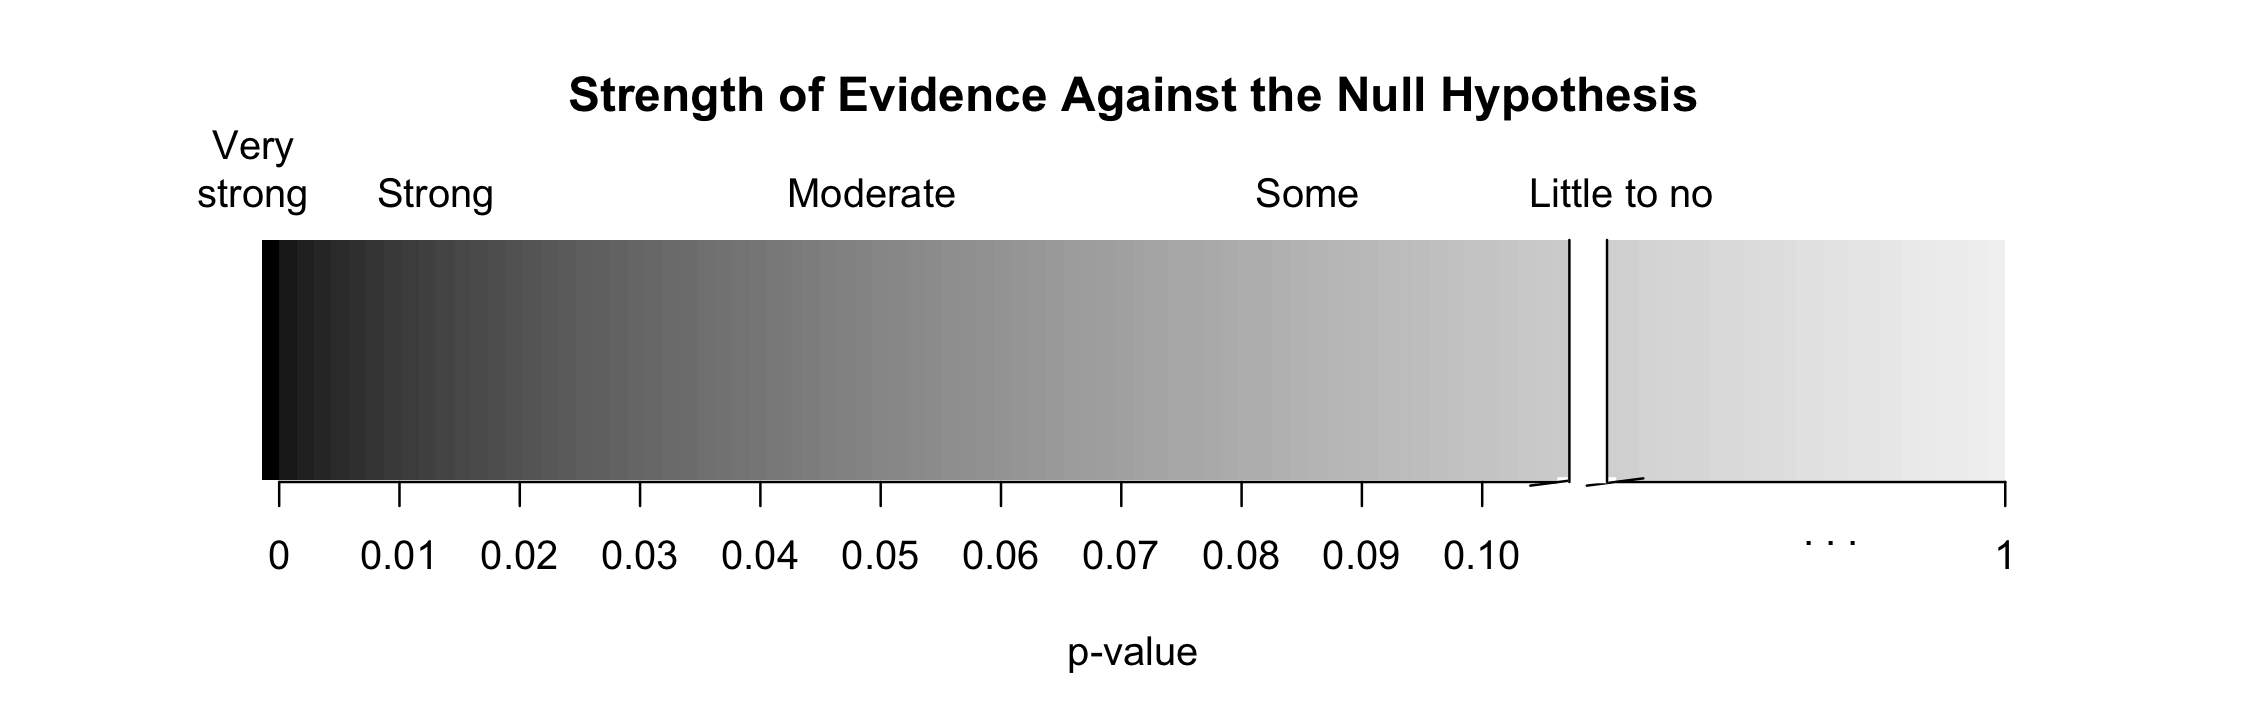
\includegraphics[width=0.9\linewidth]{images/soe_gradient_gray} \end{center}

\subsubsection*{Interpret the p-value}\label{interpret-the-p-value}
\addcontentsline{toc}{subsubsection}{Interpret the p-value}

The p-value measures the probability that we observe a sample proportion as extreme as what was seen in the data or more extreme (matching the direction of the Ha) IF the null hypothesis is true. This is a conditional probability, calculated dependent on the null hypothesis being true. Represented in probability notaton:

\[P(\text{statistic or more extreme|the null hypothesis is true})\]

\begin{enumerate}
\def\labelenumi{\arabic{enumi}.}
\setcounter{enumi}{9}
\tightlist
\item
  What did we assume to create the null distribution? Write the null hypothesis is context.
\end{enumerate}

\vspace{0.7in}

\begin{enumerate}
\def\labelenumi{\arabic{enumi}.}
\setcounter{enumi}{10}
\tightlist
\item
  What value did we compare to the null distribution to find the p-value? What is the value of the summary statistic (sample proportion)?
\end{enumerate}

\vspace{0.3in}

\begin{enumerate}
\def\labelenumi{\arabic{enumi}.}
\setcounter{enumi}{11}
\tightlist
\item
  In what direction (greater than or less than) did we count from the statistic to find the number of simulations?
  \vspace{0.3in}
\end{enumerate}

\newpage

\begin{enumerate}
\def\labelenumi{\arabic{enumi}.}
\setcounter{enumi}{12}
\tightlist
\item
  Fill in the blanks below to interpret the p-value.
\end{enumerate}

\setstretch{1.5}

We would observe a sample proportion of \hrulefill  

or (greater, less, more extreme) \hrulefill   

with a probability of \hrulefill  

IF we assume (\(H_0\) in context) \hrulefill.

\hrulefill

\setstretch{1}
\vspace{12pt}

\subsubsection*{Communicate the results and answer the research question}\label{communicate-the-results-and-answer-the-research-question}
\addcontentsline{toc}{subsubsection}{Communicate the results and answer the research question}

When we write a conclusion we answer the research question by stating how much evidence there is for the alternative hypothesis.

\begin{enumerate}
\def\labelenumi{\arabic{enumi}.}
\setcounter{enumi}{13}
\tightlist
\item
  Write a conclusion in context of the study. How much evidence does the data provide in support of the alternative hypothesis?
\end{enumerate}

\vspace{0.6in}

\setstretch{1.5}

\setstretch{1}

\subsection{Take-home messages}\label{take-home-messages-6}

\begin{enumerate}
\def\labelenumi{\arabic{enumi}.}
\item
  The null distribution is created based on the assumption the null hypothesis is true. We compare the sample statistic to the distribution to find the likelihood of observing this statistic.
\item
  The p-value measures the probability of observing the sample statistic or more extreme (in direction of the alternative hypothesis) is the null hypothesis is true.
\item
  The smaller the p-value of the test, the more evidence there is \textbf{against} the null hypothesis.
\end{enumerate}

\subsection{Additional notes}\label{additional-notes-6}

Use this space to summarize your thoughts and take additional notes on today's activity and material covered.

\newpage

\section{Activity 8: Helper-Hinderer --- Simulation-based Confidence Interval}\label{activity-8-helper-hinderer-simulation-based-confidence-interval}

\setstretch{1}

\subsection{Learning outcomes}\label{learning-outcomes-7}

\begin{itemize}
\item
  Use bootstrapping to find a confidence interval for a single proportion.
\item
  Interpret a confidence interval for a single proportion.
\end{itemize}

\subsection{Terminology review}\label{terminology-review-6}

In today's activity, we will introduce simulation-based confidence intervals for a single proportion. Some terms covered in this activity are:

\begin{itemize}
\item
  Parameter of interest
\item
  Bootstrapping
\item
  Confidence interval
\end{itemize}

To review these concepts, see Chapters 10 \& 14 in your textbook.

\subsection{Helper-Hinderer}\label{helper-hinderer-2}

In the last class, we found very strong evidence that the true proportion of infants who will choose the helper character is greater than 0.5. But what \emph{is} the true proportion of infants who will choose the helper character? We will use this same study to estimate this parameter of interest by creating a confidence interval.

As a reminder: A study by Hamblin, Wynn, and Bloom reported in Nature (Hamblin, Wynn, and Bloom 2007) was intended to check young kids' feelings about helpful and non-helpful behavior. Non-verbal infants ages 6 to 10 months were shown short videos with different shapes either helping or hindering the climber. Researchers were hoping to assess: Are infants more likely to preferentially choose the helper toy over the hinderer toy? In the study, of the 16 infants age 6 to 10 months, 14 chose the \emph{helper} toy and 2 chose the \emph{hinderer} toy.

A \textbf{point estimate} (our observed statistic) provides a single plausible value for a parameter. However, a point estimate is rarely perfect; usually there is some error in the estimate. In addition to supplying a point estimate of a parameter, a next logical step would be to provide a plausible \emph{range} of values for the parameter. This plausible range of values for the population parameter is called an \textbf{interval estimate} or \textbf{confidence interval}.

\subsubsection*{Activity intro}\label{activity-intro}
\addcontentsline{toc}{subsubsection}{Activity intro}

\begin{enumerate}
\def\labelenumi{\arabic{enumi}.}
\tightlist
\item
  What is the value of the point estimate?
\end{enumerate}

\vspace{0.3in}

\begin{enumerate}
\def\labelenumi{\arabic{enumi}.}
\setcounter{enumi}{1}
\tightlist
\item
  If we took another random sample of 16 infants, would we get the exact same point estimate? Explain why or why not.
\end{enumerate}

\vspace{0.5in}

In today's activity, we will use bootstrapping to find a 95\% confidence interval for \(\pi\), the parameter of interest.

\begin{enumerate}
\def\labelenumi{\arabic{enumi}.}
\setcounter{enumi}{2}
\tightlist
\item
  In your own words, explain the bootstrapping process.
  \vspace{0.5in}
\end{enumerate}

\subsubsection*{Use statistical analysis methods to draw inferences from the data}\label{use-statistical-analysis-methods-to-draw-inferences-from-the-data-1}
\addcontentsline{toc}{subsubsection}{Use statistical analysis methods to draw inferences from the data}

\begin{enumerate}
\def\labelenumi{\arabic{enumi}.}
\setcounter{enumi}{3}
\tightlist
\item
  Write out the parameter of interest in words, in context of the study. \emph{Hint: this is the same as in Activity 6 and 7.}
\end{enumerate}

\vspace{0.5in}

To create the null distribution we flipped a coin 16 times to simulate infants randomly choosing the helper toy with a probability of 50\%.

\begin{enumerate}
\def\labelenumi{\arabic{enumi}.}
\setcounter{enumi}{4}
\tightlist
\item
  Why can't we use a coin to simulate the bootstrap distribution.
\end{enumerate}

\vspace{0.7in}

To create the bootstrap distribution.

\begin{itemize}
\item
  First we would label the cards to represent the sample statistic: 14 helper and 2 hinderer.
\item
  Sample with replacement 16 times
\end{itemize}

\begin{enumerate}
\def\labelenumi{\arabic{enumi}.}
\setcounter{enumi}{5}
\tightlist
\item
  Using the cards provided by your instructor, create one bootstrap sample. Report your simulated sample proportion on the whiteboard.
\end{enumerate}

\vspace{0.3in}

To use the computer simulation to create a bootstrap distribution, we will need to enter the

\begin{itemize}
\tightlist
\item
  ``sample size'' (the number of observational units or cases in the sample),
\item
  ``number of successes'' (the number of cases that choose the helper character),
\item
  ``number of repetitions'' (the number of samples to be generated), and
\item
  the ``confidence level'' (which level of confidence are we using to create the confidence interval).
\end{itemize}

\begin{enumerate}
\def\labelenumi{\arabic{enumi}.}
\setcounter{enumi}{6}
\tightlist
\item
  What values should be entered for each of the following into the simulation to create the bootstrap distribution of sample proportions to find a 95\% confidence interval?
  \vspace{1mm}
\end{enumerate}

\begin{itemize}
\tightlist
\item
  Sample size:
\end{itemize}

\vspace{.1in}

\begin{itemize}
\tightlist
\item
  Number of successes:
\end{itemize}

\vspace{.1in}

\begin{itemize}
\tightlist
\item
  Number of repetitions:
\end{itemize}

\vspace{.1in}

\begin{itemize}
\tightlist
\item
  Confidence level (as a decimal):
\end{itemize}

\vspace{.1in}

We will use the \texttt{one\_proportion\_bootstrap\_CI()} function in R (in the \texttt{catstats} package) to simulate the bootstrap distribution of sample proportions and calculate a confidence interval. Using the provided R script file, fill in the values/words for each \texttt{xx} with your answers from question 5 in the one proportion bootstrap confidence interval (CI) code to create a bootstrap distribution with 10000 simulations. Then highlight and run lines 1--9.

\begin{Shaded}
\begin{Highlighting}[]
\FunctionTok{one\_proportion\_bootstrap\_CI}\NormalTok{(}\AttributeTok{sample\_size =}\NormalTok{ xx, }\CommentTok{\# Sample size}
                    \AttributeTok{number\_successes =}\NormalTok{ xx, }\CommentTok{\# Observed number of successes}
                    \AttributeTok{number\_repetitions =} \DecValTok{10000}\NormalTok{, }\CommentTok{\# Number of bootstrap samples to use}
                    \AttributeTok{confidence\_level =}\NormalTok{ xx) }\CommentTok{\# Confidence level as a decimal}
\end{Highlighting}
\end{Shaded}

\newpage

\begin{enumerate}
\def\labelenumi{\arabic{enumi}.}
\setcounter{enumi}{7}
\tightlist
\item
  Sketch the bootstrap distribution created below.
\end{enumerate}

\vspace{1.8in}

\begin{enumerate}
\def\labelenumi{\arabic{enumi}.}
\setcounter{enumi}{8}
\item
  What is the value at the center of this bootstrap distribution? Why does this make sense?
  \vspace{.8in}
\item
  Explain why the two vertical lines are at the 2.5th percentile and the 97.5th percentile.
\end{enumerate}

\vspace{.4in}

\begin{enumerate}
\def\labelenumi{\arabic{enumi}.}
\setcounter{enumi}{10}
\tightlist
\item
  Report the 95\% bootstrapped confidence interval for \(\pi\). Use interval notation: (lower value, upper value).
\end{enumerate}

\vspace{0.2in}

\begin{enumerate}
\def\labelenumi{\arabic{enumi}.}
\setcounter{enumi}{11}
\tightlist
\item
  Interpret the 95\% confidence interval in context.
\end{enumerate}

\vspace{.6in}

\subsubsection*{Communicate the results and answer the research question}\label{communicate-the-results-and-answer-the-research-question-1}
\addcontentsline{toc}{subsubsection}{Communicate the results and answer the research question}

\begin{enumerate}
\def\labelenumi{\arabic{enumi}.}
\setcounter{enumi}{12}
\tightlist
\item
  Is the value 0.5 (the null value) in the 95\% confidence interval?
\end{enumerate}

\vspace{.2in}

~~~Explain how this indicates that the p-value provides strong evidence against the null.

\vspace{0.5in}

\subsubsection*{Effect of confidence level}\label{effect-of-confidence-level}
\addcontentsline{toc}{subsubsection}{Effect of confidence level}

\begin{enumerate}
\def\labelenumi{\arabic{enumi}.}
\setcounter{enumi}{13}
\tightlist
\item
  Suppose instead of finding a 95\% confidence interval, we found a 90\% confidence interval. Would you expect the 90\% confidence interval to be narrower or wider? Explain your answer.
\end{enumerate}

\vspace{0.4in}

\begin{enumerate}
\def\labelenumi{\arabic{enumi}.}
\setcounter{enumi}{14}
\tightlist
\item
  The following R code produced the bootstrap distribution with 10000 simulations that follows. Circle the value that changed in the code.
\end{enumerate}

\begin{Shaded}
\begin{Highlighting}[]
\FunctionTok{one\_proportion\_bootstrap\_CI}\NormalTok{(}\AttributeTok{sample\_size =} \DecValTok{16}\NormalTok{, }\CommentTok{\# Sample size}
                    \AttributeTok{number\_successes =} \DecValTok{14}\NormalTok{, }\CommentTok{\# Observed number of successes}
                    \AttributeTok{number\_repetitions =} \DecValTok{10000}\NormalTok{, }\CommentTok{\# Number of bootstrap samples to use}
                    \AttributeTok{confidence\_level =} \FloatTok{0.90}\NormalTok{) }\CommentTok{\# Confidence level as a decimal}
\end{Highlighting}
\end{Shaded}

\begin{center}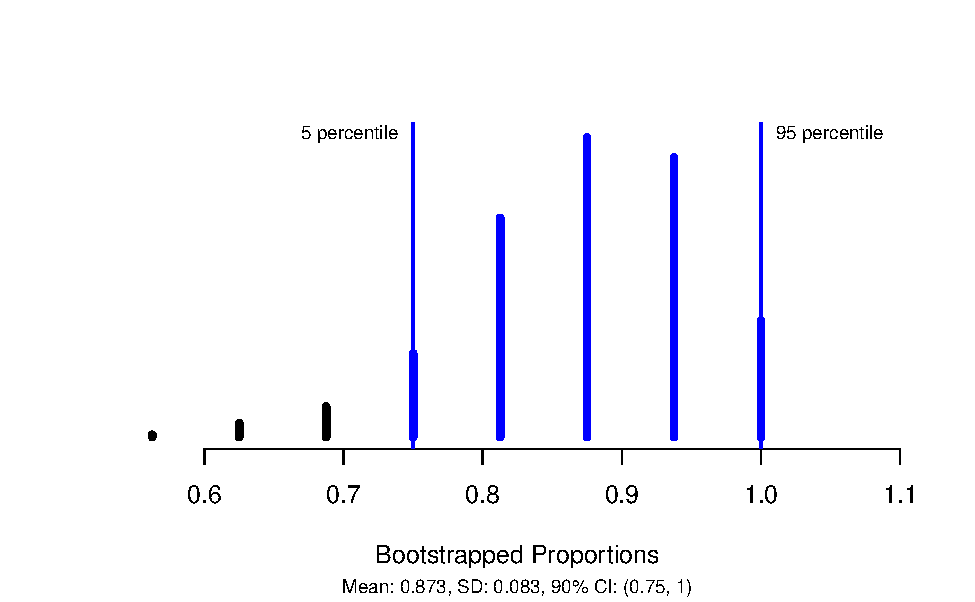
\includegraphics[width=0.7\linewidth]{03-A08-inference-1cat_CI-simulation_files/figure-latex/unnamed-chunk-2-1} \end{center}

\begin{enumerate}
\def\labelenumi{\arabic{enumi}.}
\setcounter{enumi}{15}
\tightlist
\item
  Report both the 95\% confidence interval (question 8) and the 90\% confidence interval (question 15). Is the 90\% confidence interval narrower or wider than the 95\% confidence interval?
\end{enumerate}

\vspace{0.5in}

\begin{enumerate}
\def\labelenumi{\arabic{enumi}.}
\setcounter{enumi}{16}
\tightlist
\item
  Explain why the upper value of the confidence interval is truncated at 1.
\end{enumerate}

\vspace{0.3in}

\setstretch{1.5}

\begin{enumerate}
\def\labelenumi{\arabic{enumi}.}
\setcounter{enumi}{17}
\tightlist
\item
  Fill in the blanks below to write a paragraph summarizing the results of the study as if writing a press release.
\end{enumerate}

Researchers were interested if infants observe social cues and would be more likely to choose the helper toy over the hinderer toy. In a sample of (sample size) \_\_\_\_\_\_\_\_\_\_\_\_\_infants, (number of successes) \_\_\_\_\_\_\_\_\_\_\_\_\_\_\_chose the helper toy. A simulation null distribution with 10000 simulations was created in RStudio. The p-value was found by calculating the proportion of simulations in the null distribution at the sample statistic of 0.875 and greater. This resulted in a p-value of (value of p-value)\_\_\_\_\_\_\_\_\_\_\_\_\_\_\_. We would observe a sample proportion of (value of the sample proportion) \_\_\_\_\_\_\_\_\_\_\_\_\_\_\_\_\_\_\_\_\_\_ or (greater, less, more extreme) \_\_\_\_\_\_\_\_\_\_\_\_\_\_\_\_\_\_\_\_\_ with a probability of (value of p-value)\_\_\_\_\_\_\_\_\_\_\_\_\_\_\_\_\_\_\_\\
IF we assume (\(H_0\) in context) \_\_\_\_\_\_\_\_\_\_\_\_\_\_\_\_\_\_\_\_\_\_\_\_\_\_\_\_\_\_\_\_\_\_\_\_\_\_\_\_\_\_\_\_.
Based on this p-value, there is (very strong/little to no) \_\_\_\_\_\_\_\_\_\_\_\_\_\_\_\_\_\_\_\_\_\_ evidence that the (sample/true)\_\_\_\_\_\_\_\_\_\_\_\_\_\_\_\_\_\_\_\_\_ proportion of infants age 6 to 10 months who will choose the helper toy is (greater than, less than, not equal to) \_\_\_\_\_\_\_\_\_\_\_\_\_\_\_\_\_\_\_\_\_ 0.5. In addition, a 95\% confidence interval was found for the parameter of interest. We are 95\% confident that the (true/sample)\_\_\_\_\_\_\_\_\_\_\_\_\_\_\_\_\_\_\_\_\_\_\_\_\_ proportion of infants age 6 to 10 months who will choose the helper toy is between (lower value)\_\_\_\_\_\_\_\_\_\_\_\_\_\_\_\_ and (upper value)\_\_\_\_\_\_\_\_\_\_\_\_\_\_\_\_\_\_\_\_. The results of this study can be generalized to (all infants age 6 to 10 months/infants similar to those in this study)\_\_\_\_\_\_\_\_\_\_\_\_\_\_\_\_\_\_\_\_\_\_\_\_\_\_\_ as the researchers (did/did not)\_\_\_\_\_\_\_\_\_\_\_\_\_\_\_\_\_\_\_\_\_ select a random sample.

\setstretch{1}

\subsection{Take-home messages}\label{take-home-messages-7}

\begin{enumerate}
\def\labelenumi{\arabic{enumi}.}
\item
  The goal in a hypothesis test is to assess the strength of evidence for an effect, while the goal in creating a confidence interval is to determine how large the effect is. A \textbf{confidence interval} is a range of \emph{plausible} values for the parameter of interest.
\item
  A confidence interval is built around the point estimate or observed calculated statistic from the sample. This means that the sample statistic is always the center of the confidence interval. A confidence interval includes a measure of sample to sample variability represented by the \textbf{margin of error}.
\item
  In simulation-based methods (bootstrapping), a simulated distribution of possible sample statistics is created showing the possible sample-to-sample variability. Then we find the middle \(X\) percent of the distribution around the sample statistic using the percentile method to give the range of values for the confidence interval. This shows us that we are \(X\)\% confident that the parameter is within this range, where \(X\) represents the level of confidence.
\item
  When the null value is within the confidence interval, it is a plausible value for the parameter of interest; thus, we would find a larger p-value for a hypothesis test of that null value. Conversely, if the null value is NOT within the confidence interval, we would find a small p-value for the hypothesis test and strong evidence against this null hypothesis.
\item
  To create one simulated sample on the bootstrap distribution for a sample proportion, label \(n\) cards with the original responses. Draw with replacement \(n\) times. Calculate and plot the resampled proportion of successes.
\end{enumerate}

\subsection{Additional notes}\label{additional-notes-7}

Use this space to summarize your thoughts and take additional notes on today's activity and material covered.

\newpage

\chapter{Inference for a Single Categorical Variable: Theory-based Methods}\label{inference-for-a-single-categorical-variable-theory-based-methods}

\section{Vocabulary Review and Key Topics}\label{vocabulary-review-and-key-topics-3}

Review the Golden Ticket posted in the resources at the end of the coursepack for a summary of a single categorical variable.

\subsection{Key topics}\label{key-topics-3}

Module 4 introduces theory-based inference methods (hypothesis testing and confidence intervals) for a single categorical variable. We also explore what ``confidence level'' means and which parts of a study impact the width of a confidence interval and the p-value.

\begin{itemize}
\item
  Theory-based methods should give the same results as simulation-based methods if the sample size is large enough. For a single categorical variable, the sample size is large enough if the success-failure condition is met.
\item
  If repeated samples of the same size are taken from the population, 95\% of samples will create a 95\% confidence interval that contains the value of the parameter of interest.
\end{itemize}

\subsection{Vocabulary}\label{vocabulary-3}

\begin{itemize}
\item
  \textbf{Theory-based methods}: when specific conditions are met, the distribution of sample statistics if we were to repeatedly sample from the population can be fit with a theoretical distribution.
\item
  \textbf{Conditions for the sampling distribution of \(\hat{p}\) to follow an approximate normal distribution}:

  \begin{itemize}
  \item
    \textbf{Independence}: the sample's observations are independent, e.g., are from a simple random sample. (\emph{Remember}: This also must be true to use simulation-based methods!)
  \item
    \textbf{Success-failure condition}: we \emph{expect} to see at least 10 successes and 10 failures in the sample, \(n\pi\geq10\) and \(n(1-\pi)\geq10\). Since \(\pi\) is typically unknown, we consider this condition to be met if we observe at least 10 successes and 10 failures in our data set: \(n\hat{p}\geq10\) and \(n(1-\hat{p})\geq10\).
  \end{itemize}
\item
  \textbf{Standard normal distribution}: a theoretical distribution that is bell-shaped, centered on the mean of zero, and has a standard deviation of one, denoted in notation by \(N(0,1)\).
\item
  \textbf{Standard error of a statistic}: an estimated standard deviation of the statistic as it would vary across repeated samples of the same size under the same conditions.

  \begin{itemize}
  \tightlist
  \item
    The standard error tells us about how far we would expect an observed sample statistic to fall from the true parameter value for which it is estimating, on average.
  \end{itemize}
\item
  \textbf{Standardized statistic}: calculation to standardize the sample statistic in order to compare the standardized value to the theoretical distribution.

  \begin{itemize}
  \item
    Calculated by subtracting the null value from the sample statistic, then dividing by the standard error:
    \[\frac{\text{statistic} - \text{null value}}{\text{standard error}}\]
  \item
    Measures the number of standard errors the sample statistic is above (if positive) or below (if negative) the null value.
  \end{itemize}
\item
  \textbf{Standard error of the sample proportion assuming the null is true}: measures the how far each possible sample proportion is from the true proportion, on average, and is calculated using the null value:
\end{itemize}

\[SE_0(\hat{p})=\sqrt{\frac{\pi_0\times(1-\pi_0)}{n}}\].

\begin{itemize}
\item
  \textbf{Standardized sample proportion}: standardized statistic for a single categorical variable calculated using:
  \[
  Z = \frac{\hat{p} - \pi_0}{SE_0(\hat{p})},
  \]
  If the conditions for the sampling distribution of \(\hat{p}\) to follow an approximate normal distribution are met, and if the true value of \(\pi\) is equal to the null value of \(\pi_0\), the standardized sample proportion, \(Z\), will have an approximate \emph{standard} normal distribution.
\item
  The theory-based \textbf{p-value} for hypothesis testing involving proportions can be found in R by using the \texttt{pnorm} function to find the probability of the observed standardized statistic or one more extreme (in the direction of \(H_A\)). This probability is the area under a \emph{standard normal distribution} at or more extreme than the observed standardized statistic.

  \begin{itemize}
  \item
    Enter the value of the standardized statistic for \texttt{xx}.
  \item
    If a ``greater than'' alternative, change \texttt{lower.tail\ =\ TRUE} to \texttt{FALSE}.
  \item
    If a two-sided test, multiply by 2.
  \end{itemize}

\begin{Shaded}
\begin{Highlighting}[]
\FunctionTok{pnorm}\NormalTok{(xx, }\AttributeTok{lower.tail=}\ConstantTok{TRUE}\NormalTok{)}
\end{Highlighting}
\end{Shaded}
\item
  \textbf{Margin of error}: half the width of the confidence interval. For a single proportion, the margin of error is:
  \[ME = z^* \times SE(\hat{p})\]
  where \(z^*\) is the \textbf{multiplier}, corresponding to the desired confidence level found from the standard normal distribution. For example, for a 95\% confidence level, the middle 95\% of the standard normal distribution falls between \(-z^*=-1.96\) and \(z^*=1.96\).
\item
  \textbf{Standard error of the sample proportion for a confidence interval} (not assuming the null is true):
  \[SE(\hat{p}) = \sqrt{\frac{\hat{p}\times (1-\hat{p})}{n}}\]
\item
  To find the endpoints of a confidence interval, add and subtract the margin of error to the sample statistic. The confidence interval for a population proportion is:
\end{itemize}

\[\hat{p} \pm ME\]

\begin{itemize}
\item
  R code to find the \textbf{multiplier} for the confidence interval using theory-based methods involving proportions.

  \begin{itemize}
  \item
    \texttt{qnorm} will give you the multiplier using the standard normal distribution.
  \item
    Enter the percentile for the given level of confidence (e.g., 0.975 for a 95\% confidence level).
  \end{itemize}

\begin{Shaded}
\begin{Highlighting}[]
\FunctionTok{qnorm}\NormalTok{(percentile, }\AttributeTok{lower.tail=}\ConstantTok{TRUE}\NormalTok{)}
\end{Highlighting}
\end{Shaded}
\end{itemize}

\newpage

\section{Video Notes: Inference for One Categorical Variable using Theory-based Methods}\label{video-notes-inference-for-one-categorical-variable-using-theory-based-methods}

Read Chapter 11 and Sections 14.3 and 14.4 in the course textbook. Use the following videos to complete the video notes for Module 4.

\subsection{Course Videos}\label{course-videos-3}

\begin{itemize}
\item
  Chapter11
\item
  14.3TheoryTests
\item
  14.3TheoryIntervals
\end{itemize}

\setstretch{1}

\subsection*{Theory-based methods}\label{theory-based-methods}
\addcontentsline{toc}{subsection}{Theory-based methods}

\subsubsection*{Central limit theorem - Video Chapter11}\label{central-limit-theorem---video-chapter11}
\addcontentsline{toc}{subsubsection}{Central limit theorem - Video Chapter11}

The Central Limit Theorem tells us that the \_\_\_\_\_\_\_\_\_\_\_\_\_\_ distribution of a sample proportion (and sample mean and sample differences) will be approximately \_\_\_\_\_\_\_\_\_\_\_\_\_\_ if the sample size is \_\_\_\_\_\_\_\_\_\_\_\_\_\_ \_\_\_\_\_\_\_\_\_\_\_\_\_\_\_\_.

The \_\_\_\_\_\_\_\_\_\_\_\_\_\_ of the distribution of sample proportions (sampling distribution) from thousands of samples will be bell-shaped/symmetric (Normal), if the sample size is large enough and the observations are \_\_\_\_\_\_\_\_\_\_\_\_\_\_\_\_.

\begin{itemize}
\tightlist
\item
  \(\hat{p} \sim N (\pi, \sqrt{\frac{\pi \times (1-\pi)}{n}})\)
\end{itemize}

Conditions of the CLT:

\begin{itemize}
\tightlist
\item
  Independence (\emph{also must be met to use simulation methods}): the response for one observational unit will not influence another observational unit
\end{itemize}

\vspace{1mm}

\begin{itemize}
\tightlist
\item
  Large enough sample size:
\end{itemize}

\vspace{0.3in}

Normal distribution:

\begin{itemize}
\item
  Bell-shaped and \_\_\_\_\_\_\_\_\_\_\_\_\_\_
\item
  Standard normal distribution: \(N(0,1)\)
\end{itemize}

\begin{center}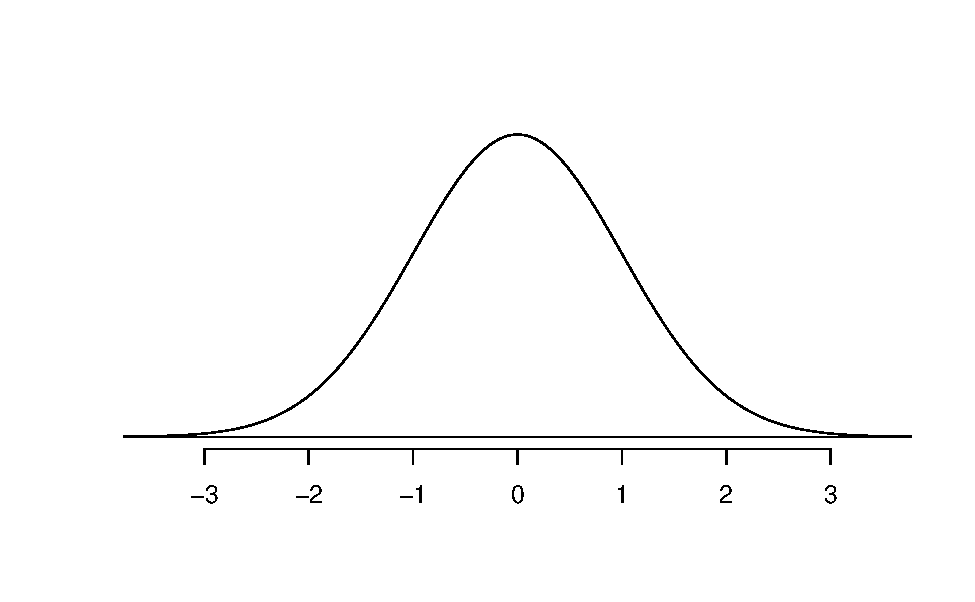
\includegraphics[width=0.45\linewidth]{04-VN04-1cat_theory_files/figure-latex/simpleNormalc-1} \end{center}

\newpage

Standardized statistic: Z - score

\vspace{1mm}

\begin{itemize}
\tightlist
\item
  \(Z = \frac{\mbox{statistic} - \mbox{null value}}{\mbox{standard error of the statistic}}\)
\end{itemize}

\vspace{0.5in}

\begin{itemize}
\tightlist
\item
  Measures the \_\_\_\_\_\_\_\_\_\_\_ of standard \_\_\_\_\_\_\_\_\_\_\_\_\_ the statistic is from the null value
\end{itemize}

Example(s): Heights of Caucasian American adult males are roughly Normally distributed with a mean of 1.72 m and a standard deviation of 0.28 m. Find and interpret the z-score for a man who is 5'4'' (1.626 m) tall. Round your answer to three decimal places.

\vspace{0.6in}

Heights of Caucasian American adult females are roughly Normally distributed with a mean of 1.59 meters and a standard deviation of 0.22 meters. Which is more unusual: a 5'4'' (1.626 m) tall male or a 5'9'' (1.753 m) tall female?

\vspace{0.6in}

In a Normal curve, the area under the curve is equal to 1, representing a probability. Therefore the shaded area represents the probability of a man being under 1.626 meters tall.

\begin{Shaded}
\begin{Highlighting}[]
\FunctionTok{library}\NormalTok{(openintro)}
\FunctionTok{normTail}\NormalTok{(}\AttributeTok{m =} \FloatTok{1.72}\NormalTok{, }\AttributeTok{s =} \FloatTok{0.28}\NormalTok{, }\AttributeTok{L =} \FloatTok{1.626}\NormalTok{)}
\FunctionTok{pnorm}\NormalTok{(}\AttributeTok{mean =} \FloatTok{1.72}\NormalTok{, }\AttributeTok{sd =} \FloatTok{0.28}\NormalTok{, }\AttributeTok{q =} \FloatTok{1.626}\NormalTok{)}
\CommentTok{\#\textgreater{} [1] 0.3685432}
\end{Highlighting}
\end{Shaded}

\begin{center}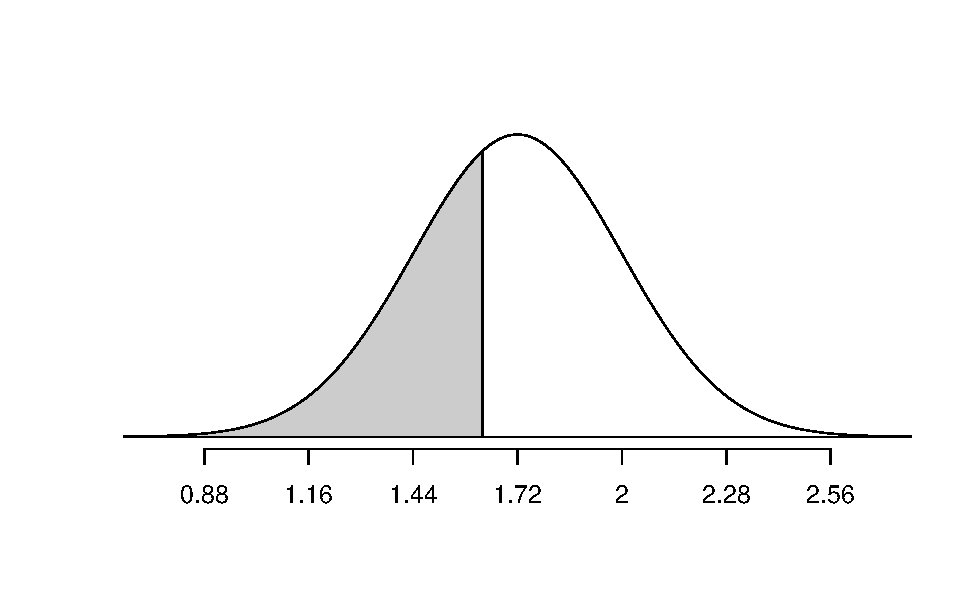
\includegraphics[width=0.6\linewidth]{04-VN04-1cat_theory_files/figure-latex/unnamed-chunk-1-1} \end{center}

\vspace{1mm}

We can also reverse that order. Given a percentage, we can find the associated percentile, or quantile. Here we display calculating the value that cuts off the lower 0.75 proportion of male adult Caucasian heights using the qnorm() function.

\begin{Shaded}
\begin{Highlighting}[]
\FunctionTok{qnorm}\NormalTok{(}\AttributeTok{mean =} \FloatTok{1.72}\NormalTok{, }\AttributeTok{sd =} \FloatTok{0.28}\NormalTok{, }\AttributeTok{p =} \FloatTok{0.75}\NormalTok{)}
\CommentTok{\#\textgreater{} [1] 1.908857}
\FunctionTok{normTail}\NormalTok{(}\AttributeTok{m =} \FloatTok{1.72}\NormalTok{, }\AttributeTok{s =} \FloatTok{0.28}\NormalTok{, }\AttributeTok{L =} \FloatTok{1.909}\NormalTok{)}
\end{Highlighting}
\end{Shaded}

\begin{center}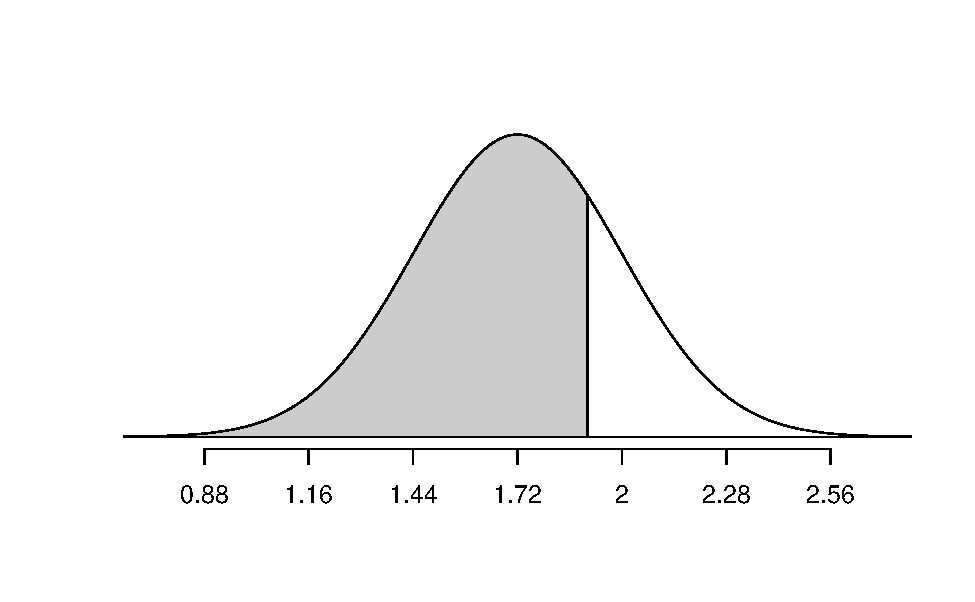
\includegraphics[width=0.6\linewidth]{04-VN04-1cat_theory_files/figure-latex/unnamed-chunk-2-1} \end{center}

\subsection*{68-95-99.7 Rule}\label{rule}
\addcontentsline{toc}{subsection}{68-95-99.7 Rule}

\begin{itemize}
\item
  68\% of Normal distribution within 1 SD of the mean (mean -- SD, mean + SD)
\item
  95\% within (mean -- 2SD, mean + 2SD)
\item
  99.7\% within (mean -- 3SD, mean + 3SD)
\end{itemize}

\begin{center}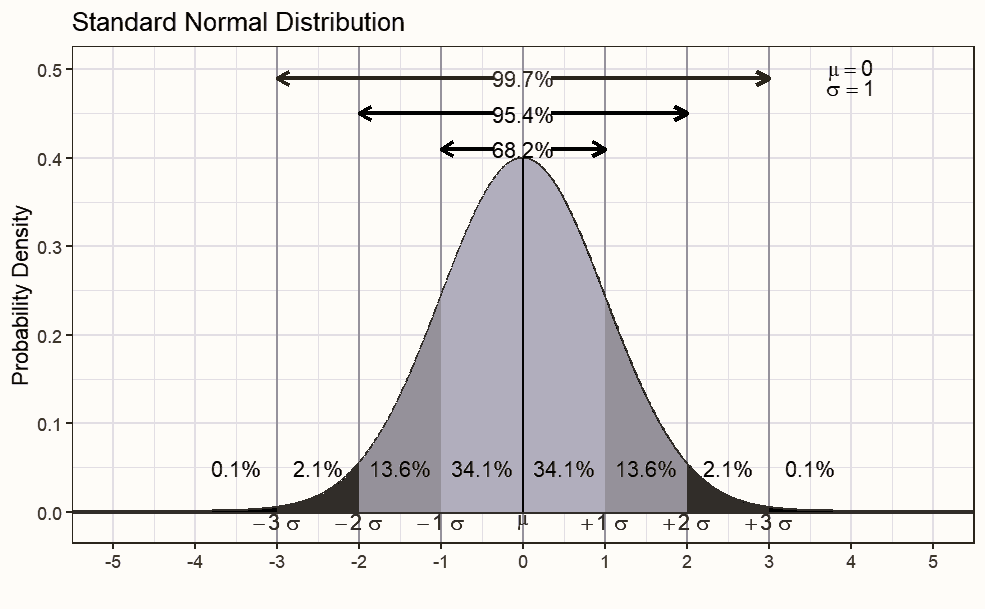
\includegraphics[width=0.65\linewidth]{images/Empirical_Rule_Mark_bw} \end{center}

General steps of a hypothesis test

\begin{enumerate}
\def\labelenumi{\arabic{enumi}.}
\item
  Write a research question and hypotheses.
\item
  Collect data and calculate a summary statistic.
\item
  Model a sampling distribution which assumes the null hypothesis is true.
\item
  Calculate a p-value.
\item
  Draw conclusions based on a p-value.
\end{enumerate}

\newpage

\subsubsection*{Example in Video 14.3TheoryTests}\label{example-in-video-14.3theorytests}
\addcontentsline{toc}{subsubsection}{Example in Video 14.3TheoryTests}

Example: The American Red Cross reports that 10\% of US residents eligible to donate blood actually do donate. A poll conducted on a representative of 200 Montana residents eligible to donate blood found that 33 had donated blood sometime in their life. Do Montana residents donate at a different rate than US population?

Hypotheses:

In notation:

\(H_0:\)

\vspace{0.2in}

\(H_A:\)

\vspace{0.2in}

Parameter of interest:

\vspace{0.6in}

Conditions for inference using theory-based methods:

\begin{itemize}
\item
  Independence:

  \begin{itemize}
  \tightlist
  \item
    The outcome of one observation does not influence the outcome of another.
  \item
    Taking a random sample is one way to satisfy this condition.
  \end{itemize}
\item
  Large enough sample size:
\end{itemize}

\vspace{1in}

Are the conditions met to analyze the blood donations data using theory-based methods?

\vspace{1in}

To use theory-based methods to perform a hypothesis test:

\begin{itemize}
\item
  1st: Calculate the standardized statistic
\item
  2nd: Find the area under the standard normal distribution at least as extreme as the standardized statistic
\end{itemize}

Equation for the standard error of the sample proportion assuming the null hypothesis is true:

\vspace{0.5in}

\setstretch{1.5}

\begin{itemize}
\tightlist
\item
  This value measures how far each possible sample statistic is from the null value, on average.
\end{itemize}

\setstretch{1}

Equation for the standardized sample proportion:

\vspace{0.5in}

\setstretch{1.5}

\begin{itemize}
\tightlist
\item
  This value measures how many standard deviations the sample proportion is above/below the null value.
\end{itemize}

\setstretch{1}

Calculate the standardized sample proportion of Montana residents that have donated blood sometime in their life.

\begin{itemize}
\tightlist
\item
  First calculate the standard error of the sample proportion assuming the null hypothesis is true
\end{itemize}

\vspace{0.5in}

\begin{itemize}
\tightlist
\item
  Then calculate the Z score.
\end{itemize}

\vspace{0.5in}

\begin{center}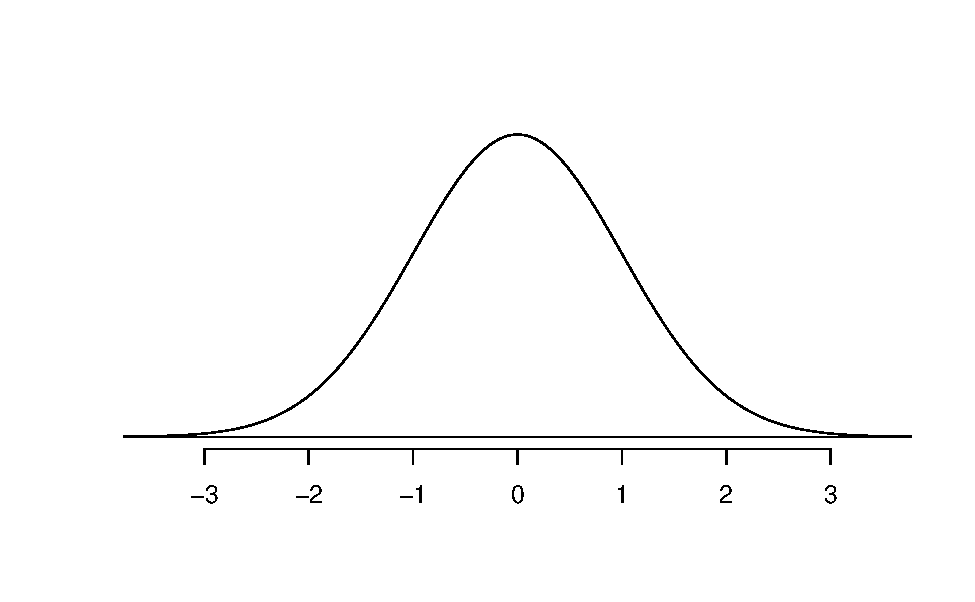
\includegraphics[width=0.5\linewidth]{04-VN04-1cat_theory_files/figure-latex/standNormalc-1} \end{center}

Interpret the standardized statistic

\vspace{0.5in}

To find the p-value, find the area under the standard normal distribution at the standardized statistic and more extreme.

\begin{Shaded}
\begin{Highlighting}[]
\FunctionTok{pnorm}\NormalTok{(}\FloatTok{3.064}\NormalTok{, }\AttributeTok{lower.tail =} \ConstantTok{FALSE}\NormalTok{)}\SpecialCharTok{*}\DecValTok{2}
\end{Highlighting}
\end{Shaded}

\begin{verbatim}
#> [1] 0.002183989
\end{verbatim}

Interpretation of the p-value:

\begin{itemize}
\item
  Statement about probability or proportion of samples
\item
  Statistic (summary measure and value)
\item
  Direction of the alternative
\item
  Null hypothesis (in context)
\end{itemize}

\vspace{0.6in}

Conclusion:

\begin{itemize}
\item
  Amount of evidence
\item
  Parameter of interest
\item
  Direction of the alternative hypothesis
\end{itemize}

\vspace{0.5in}

Decision at a significance level of 0.05 \((\alpha = 0.05)\):

\vspace{0.3in}

Generalization:

\begin{itemize}
\tightlist
\item
  Can the results of the study be generalized to the target population?
\end{itemize}

\vspace{0.4in}

\subsection*{Confidence interval - 14.3TheoryIntervals}\label{confidence-interval---14.3theoryintervals}
\addcontentsline{toc}{subsection}{Confidence interval - 14.3TheoryIntervals}

\begin{itemize}
\item
  Interval of \_\_\_\_\_\_\_\_\_\_ values for the parameter of interest
\item
  \(CI = \text{statistic} \pm \text{margin of error}\)
\end{itemize}

\vspace{0.5in}

\subsubsection*{Theory-based method for a single categorical variable}\label{theory-based-method-for-a-single-categorical-variable}
\addcontentsline{toc}{subsubsection}{Theory-based method for a single categorical variable}

\begin{itemize}
\item
  \(CI = \hat{p} \pm (z^* \times SE(\hat{p}))\)
\item
  Multiplier (\(z^*\)) is the value at a certain \_\_\_\_\_\_\_\_\_\_\_\_ under the standard normal distribution
\end{itemize}

\begin{center}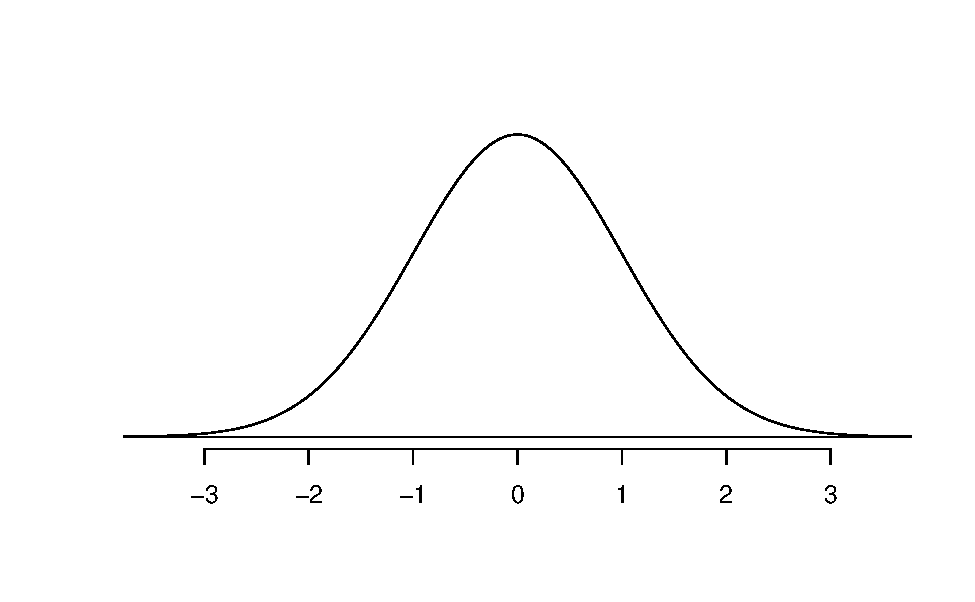
\includegraphics[width=0.5\linewidth]{04-VN04-1cat_theory_files/figure-latex/standardNormalcur-1} \end{center}

For a 95\% confidence interval:

\begin{Shaded}
\begin{Highlighting}[]
\FunctionTok{qnorm}\NormalTok{(}\FloatTok{0.975}\NormalTok{, }\AttributeTok{lower.tail=}\ConstantTok{TRUE}\NormalTok{)}
\end{Highlighting}
\end{Shaded}

\begin{verbatim}
#> [1] 1.959964
\end{verbatim}

\setstretch{1.5}

\begin{itemize}
\tightlist
\item
  When creating a confidence interval, we no longer assume the \_\_\_\_\_\_\_\_\_\_\_\_\_ hypothesis is true. Use \_\_\_\_\_\_\_\_ to calculate the sample to sample variability, rather than \(\pi_0\).
\end{itemize}

\setstretch{1}

Equation for the standard error of the sample proportion \emph{NOT} assuming the null is true:

\vspace{0.5in}

\newpage

Example: Estimate the true proportion of Montana residents that have donated blood at least once in their life.

Find a 95\% confidence interval:

\vspace{1in}

Confidence interval interpretation:

\begin{itemize}
\item
  How confident you are (e.g., 90\%, 95\%, 98\%, 99\%)
\item
  Parameter of interest
\item
  Calculated interval
\item
  Order of subtraction when comparing two groups
\end{itemize}

\vspace{0.8in}

\subsubsection*{Interpreting confidence level}\label{interpreting-confidence-level}
\addcontentsline{toc}{subsubsection}{Interpreting confidence level}

\setstretch{1.5}

What does it mean to be 95\% confident in a created confidence interval?

\begin{itemize}
\item
  Our goal is to only take one sample from the population to create a confidence interval.
\item
  Based on the 68-95-99.7 rule, we know that approximately \_\_\_\_\_\_\% of sample \_\_\_\_\_\_\_\_\_\_\_\_\_\_ will fall within \_\_\_\_\_\_\_\_\_\_ from the parameter.
\item
  If we create 95\% confidence intervals, \_\_\_\_\_\_\_\_\% of samples will create a 95\% \_\_\_\_\_\_\_\_\_\_\_\_\_\_ interval that will contain the \_\_\_\_\_\_\_\_\_\_\_\_\_ of interest.
\item
  95\% of samples accurately \_\_\_\_\_\_\_\_\_\_\_\_\_\_ the parameter of interest

  \begin{itemize}
  \tightlist
  \item
    When we create one confidence interval, we are 95\% \_\_\_\_\_\_\_\_\_\_\_\_\_\_\_\_ that we have a ``good'' sample that created a confidence interval that contains the \_\_\_\_\_\_\_\_\_\_\_ of interest.
  \end{itemize}
\end{itemize}

\setstretch{1}

Interpret the confidence \textbf{level} for the blood donation study.

\vspace{0.5in}

\newpage

\subsection{Concept Check}\label{concept-check-4}

Be prepared for group discussion in the next class. One member from the table should write the answers to the following on the whiteboard.

\begin{enumerate}
\def\labelenumi{\arabic{enumi}.}
\tightlist
\item
  What conditions must be met to use the Normal Distribution to approximate the sampling distribution of sampling proportions?
\end{enumerate}

\vspace{0.6in}

\begin{enumerate}
\def\labelenumi{\arabic{enumi}.}
\setcounter{enumi}{1}
\tightlist
\item
  Should the conclusion include a population word like \emph{true} or \emph{long-run}? Explain your answer.
\end{enumerate}

\vspace{0.6in}

\newpage

\section{Activity 9: Handedness of Male Boxers}\label{activity-9-handedness-of-male-boxers}

\setstretch{1}

\subsection{Learning outcomes}\label{learning-outcomes-8}

\begin{itemize}
\item
  Describe and perform a theory-based hypothesis test for a single proportion.
\item
  Check the appropriate conditions to use a theory-based hypothesis test.
\item
  Calculate and interpret the standardized sample proportion.
\item
  Interpret and evaluate a p-value for a theory-based hypothesis test for a single proportion.
\item
  Use the normal distribution to find the p-value.
\end{itemize}

\subsection{Terminology review}\label{terminology-review-7}

In this activity, we will introduce theory-based hypothesis tests for a single categorical variable. Some terms covered in this activity are:

\begin{itemize}
\item
  Parameter of interest
\item
  Standardized statistic
\item
  Normal distribution
\item
  p-value
\end{itemize}

To review these concepts, see Chapter 11 \& 14 in your textbook.

Activities from module 5 covered simulation-based methods for hypothesis tests involving a single categorical variable. This activity covers theory-based methods for testing a single categorical variable.

\subsection{Handedness of male boxers}\label{handedness-of-male-boxers}

Left-handedness is a trait that is found in about 10\% of the general population. Past studies have shown that left-handed men are over-represented among professional boxers (Richardson and Gilman 2019). The fighting claim states that left-handed men have an advantage in competition. In this random sample of 500 male professional boxers, we want to see if there is an over-prevalence of left-handed fighters. In the sample of 500 male boxers, 81 were left-handed.

\subsection{Summary statistics review}\label{summary-statistics-review}

\begin{itemize}
\item
  Download the R file for today's activity from D2L
\item
  Upload the file to the R server
\item
  Run lines 1--15 to load the needed packages and the data set and create a plot of the data
\end{itemize}

\begin{Shaded}
\begin{Highlighting}[]
 \CommentTok{\# Read in data set}
\NormalTok{boxers }\OtherTok{\textless{}{-}} \FunctionTok{read.csv}\NormalTok{(}\StringTok{"https://math.montana.edu/courses/s216/data/Male\_boxers\_sample.csv"}\NormalTok{)}
\NormalTok{boxers }\SpecialCharTok{\%\textgreater{}\%} \FunctionTok{count}\NormalTok{(Stance)  }\CommentTok{\# Count number in each Stance category}
\end{Highlighting}
\end{Shaded}

\begin{verbatim}
#>         Stance   n
#> 1  left-handed  81
#> 2 right-handed 419
\end{verbatim}

\newpage

\begin{Shaded}
\begin{Highlighting}[]
\NormalTok{boxers }\SpecialCharTok{\%\textgreater{}\%} \CommentTok{\# Data set piped into...}
    \FunctionTok{ggplot}\NormalTok{(}\FunctionTok{aes}\NormalTok{(}\AttributeTok{x =}\NormalTok{ Stance)) }\SpecialCharTok{+}   \CommentTok{\# This specifies the variable}
    \FunctionTok{geom\_bar}\NormalTok{(}\FunctionTok{aes}\NormalTok{(}\AttributeTok{y =} \FunctionTok{after\_stat}\NormalTok{(prop), }\AttributeTok{group =} \DecValTok{1}\NormalTok{)) }\SpecialCharTok{+}  \CommentTok{\# Tell it to make a bar plot with proportions}
    \FunctionTok{labs}\NormalTok{(}\AttributeTok{title =} \StringTok{"\_\_\_\_\_\_\_\_\_\_\_\_\_\_\_\_\_\_\_\_ of Handedness of Male Professional Boxers"}\NormalTok{,  }
       \CommentTok{\# Give your plot a title}
       \AttributeTok{x =} \StringTok{"Handedness"}\NormalTok{,   }\CommentTok{\# Label the x axis}
       \AttributeTok{y =} \StringTok{"Relative Frequency"}\NormalTok{)  }\CommentTok{\# Label the y axis}
\end{Highlighting}
\end{Shaded}

\begin{center}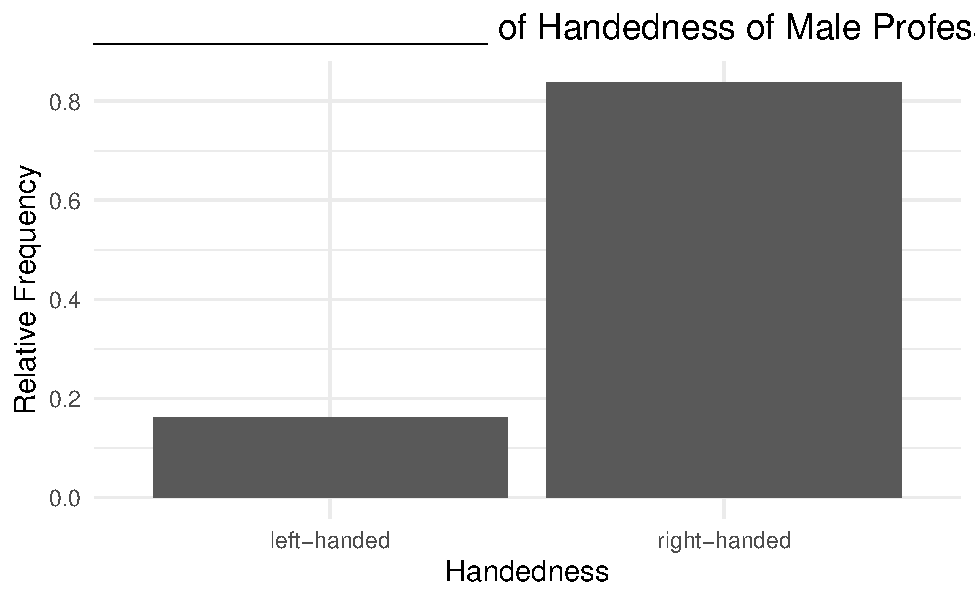
\includegraphics[width=0.5\linewidth]{04-A09-inference-1cat-theory_files/figure-latex/unnamed-chunk-2-1} \end{center}

\begin{enumerate}
\def\labelenumi{\arabic{enumi}.}
\tightlist
\item
  What type of plot was created of these data?
\end{enumerate}

\vspace{0.2in}

\subsection*{Hypotheses and summary statistics}\label{hypotheses-and-summary-statistics}
\addcontentsline{toc}{subsection}{Hypotheses and summary statistics}

\begin{enumerate}
\def\labelenumi{\arabic{enumi}.}
\setcounter{enumi}{1}
\tightlist
\item
  Write out the parameter of interest in words, in context of the study.
\end{enumerate}

\vspace{1in}

\begin{enumerate}
\def\labelenumi{\arabic{enumi}.}
\setcounter{enumi}{2}
\item
  Write out the null hypothesis in words.
  \vspace{1in}
\item
  Write out the alternative hypothesis in notation.
  \vspace{0.4in}
\item
  Give the value of the summary statistic (sample proportion) for this study. Use proper notation.
\end{enumerate}

\vspace{0.3in}

\newpage

\subsection*{Theory-based methods}\label{theory-based-methods-1}
\addcontentsline{toc}{subsection}{Theory-based methods}

The sampling distribution of a single proportion --- how that proportion varies from sample to sample --- can be mathematically modeled using the normal distribution if certain conditions are met.

Conditions for the sampling distribution of \(\hat{p}\) to follow an approximate normal distribution:

\begin{itemize}
\item
  \textbf{Independence}: The sample's observations are independent, e.g., are from a simple random sample. (\emph{Remember}: This also must be true to use simulation methods!)
\item
  \textbf{Success-failure condition}: We \emph{expect} to see at least 10 successes and 10 failures in the sample, \(n\hat{p}≥10\) and \(n(1-\hat{p})≥10\).
\end{itemize}

\begin{enumerate}
\def\labelenumi{\arabic{enumi}.}
\setcounter{enumi}{5}
\tightlist
\item
  Verify that the independence condition is satisfied.
\end{enumerate}

\vspace{0.5in}

\begin{enumerate}
\def\labelenumi{\arabic{enumi}.}
\setcounter{enumi}{6}
\tightlist
\item
  Is the success-failure condition met to model the data with the normal distribution? Explain your answer in context of the problem.
\end{enumerate}

\vspace{0.8in}

To calculate the standardized statistic we use the general formula

\[
Z = \frac{\text{point estimate} - \text{null value}}{SE_0(\text{point estimate})}.
\]
For a single categorical variable the standardized sample proportion is calculated using

\[
Z = \frac{\hat{p} - \pi_0}{SE_0(\hat{p})},
\]
where the standard error is calculated using the null value:

\[SE_0(\hat{p})=\sqrt{\frac{\pi_0\times(1-\pi_0)}{n}}\].

For this study, the null standard error of the sample proportion is calculated using the null value, 0.1.

\[SE_0(\hat{p})=\sqrt{\frac{0.1\times(1-0.1)}{500}} = 0.013\].

Each sample proportion of male boxers that are left-handed is 0.013 from the true proportion of male boxers that are left-handed, on average.

\newpage

\begin{enumerate}
\def\labelenumi{\arabic{enumi}.}
\setcounter{enumi}{7}
\tightlist
\item
  Label the standard normal distribution shown below with the null value as the center value (below the value of zero). Label the tick marks to the right of the null value by adding 1 standard error to the null value to represent 1 standard error, 2 standard errors, and 3 standard errors from the null. Repeat this process to the left of the null value by subtracting 1 standard error for each tick mark.
\end{enumerate}

\vspace{2mm}

\begin{figure}

{\centering 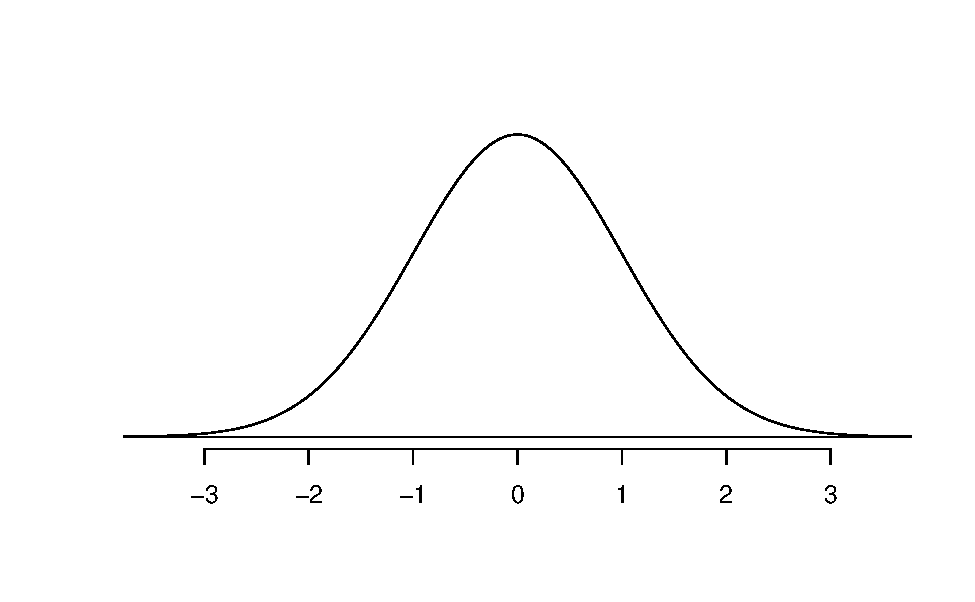
\includegraphics[width=0.5\linewidth]{04-A09-inference-1cat-theory_files/figure-latex/Normcur-1} 

}

\caption{Standard Normal Curve}\label{fig:Normcur}
\end{figure}

\begin{enumerate}
\def\labelenumi{\arabic{enumi}.}
\setcounter{enumi}{8}
\tightlist
\item
  Using the null standard error of the sample proportion, calculate the standardized sample proportion (Z). Mark this value on the standard normal distribution above.
\end{enumerate}

\vspace{0.6in}

The standardized statistic is used as a ruler to measure how far the sample statistic is from the null value. Essentially, we are converting the sample proportion into a measure of standard errors to compare to the standard normal distribution.

The standardized statistic measures the \emph{number of standard errors the sample statistic is from the null value}.

\begin{enumerate}
\def\labelenumi{\arabic{enumi}.}
\setcounter{enumi}{9}
\tightlist
\item
  Interpret the standardized sample proportion from question 9 in context of the problem.
\end{enumerate}

\vspace{.8in}

We will use the \texttt{pnorm()} function in \texttt{R} to find the p-value. In the code below, notice that we used \texttt{lower.tail\ =\ FALSE} to find the p-value. \texttt{R} will calculate the p-value \emph{greater} than the value of the standardized statistic.

Notes:

\begin{itemize}
\item
  Use \texttt{lower.tail\ =\ TRUE} when doing a left-sided test.
\item
  Use \texttt{lower.tail\ =\ FALSE} when doing a right-sided test.
\item
  To find a two-sided p-value, use a left-sided test for negative Z or a right-sided test for positive Z, then multiply the value found by 2 to get the p-value.
\item
  Enter the value of the standardized statistic for xx
\item
  Highlight and run lines 20--22
\end{itemize}

\begin{Shaded}
\begin{Highlighting}[]
\FunctionTok{pnorm}\NormalTok{(xx, }\CommentTok{\# Enter value of standardized statistic}
      \AttributeTok{m=}\DecValTok{0}\NormalTok{, }\AttributeTok{s=}\DecValTok{1}\NormalTok{, }\CommentTok{\# Using the standard normal mean = 0, sd = 1}
      \AttributeTok{lower.tail=}\ConstantTok{FALSE}\NormalTok{) }\CommentTok{\# Gives a p{-}value greater than the standardized statistic}
\end{Highlighting}
\end{Shaded}

\begin{enumerate}
\def\labelenumi{\arabic{enumi}.}
\setcounter{enumi}{10}
\item
  Report the p-value obtained from the \texttt{R} output.
  \vspace{0.3in}
\item
  Write a conclusion based on the value of the p-value.
\end{enumerate}

\vspace{0.6in}

\subsection*{Impacts on the P-value}\label{impacts-on-the-p-value}
\addcontentsline{toc}{subsection}{Impacts on the P-value}

Suppose that we want to show that the true proportion of male boxers \textbf{differs} from that in the general population.

\begin{enumerate}
\def\labelenumi{\arabic{enumi}.}
\setcounter{enumi}{12}
\tightlist
\item
  Write out the alternative hypothesis in notation for this new research question.
\end{enumerate}

\vspace{0.3in}

\begin{enumerate}
\def\labelenumi{\arabic{enumi}.}
\setcounter{enumi}{13}
\tightlist
\item
  How would this impact the p-value? Would the p-value be larger or smaller?
\end{enumerate}

\vspace{0.2in}

\begin{enumerate}
\def\labelenumi{\arabic{enumi}.}
\setcounter{enumi}{14}
\tightlist
\item
  Suppose instead of 500 male boxers the researchers only took a sample of 300 male boxers and found the same proportion (\(\hat{p}=0.162\)) of male boxers that are left-handed. Since we are still assuming the same null value, 0.1, the standard error would be calculated as below:
\end{enumerate}

\[SE_0(\hat{p})=\sqrt{\frac{0.1(1-0.1)}{300}} = 0.017\].

The standardized statistic for this new sample is calculated below:

\[Z = \frac{0.162-0.1}{0.017} = 3.64\]

\begin{enumerate}
\def\labelenumi{\arabic{enumi}.}
\setcounter{enumi}{15}
\tightlist
\item
  Mark the value of the original standardized statistic from question 9 and the value of the standardized statistic from the smaller sample size on the standard normal distribution below.
\end{enumerate}

\begin{figure}

{\centering 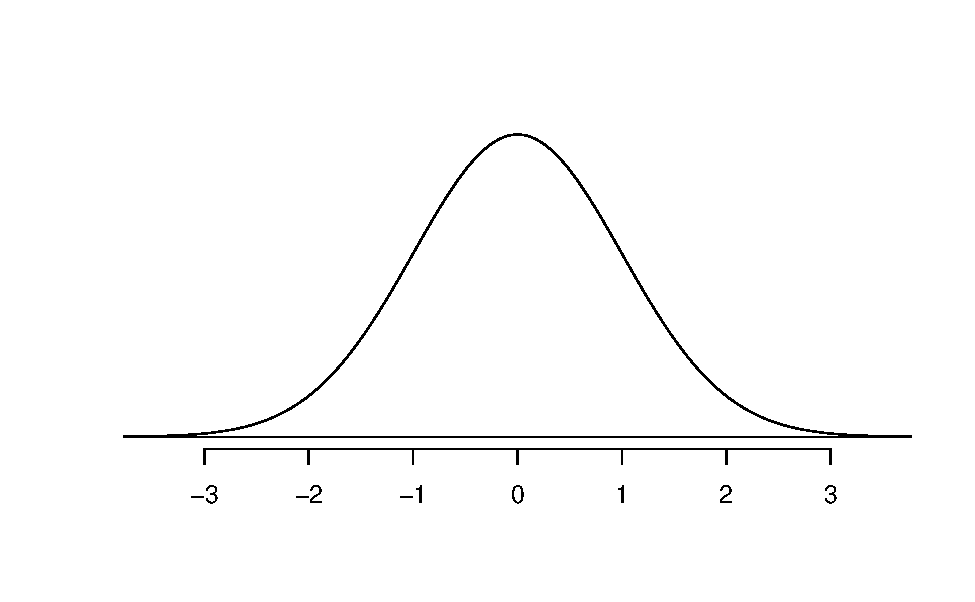
\includegraphics[width=0.5\linewidth]{04-A09-inference-1cat-theory_files/figure-latex/Norcur-1} 

}

\caption{Standard Normal Curve}\label{fig:Norcur}
\end{figure}

\newpage

\begin{enumerate}
\def\labelenumi{\arabic{enumi}.}
\setcounter{enumi}{16}
\tightlist
\item
  How does the decrease in sample size affect the p-value?
\end{enumerate}

\vspace{0.3in}

\begin{enumerate}
\def\labelenumi{\arabic{enumi}.}
\setcounter{enumi}{17}
\tightlist
\item
  Suppose another sample of 500 male boxers was taken and 68 were found to be left-handed. Since we are still assuming the same null value, 0.1, the standard error would be calculated as before:
\end{enumerate}

\[SE_0(\hat{p})=\sqrt{\frac{0.1(1-0.1)}{500}} = 0.013\].

The standardized statistic for this new sample is calculated below:

\[Z = \frac{0.136-0.1}{0.013} = 2.769\]
19. Mark the Z-value of the original standardized statistic from question 9 and the value of the standardized statistic calculated with \(\hat{p}=0.136\) on the standard normal distribution below.

\begin{figure}

{\centering 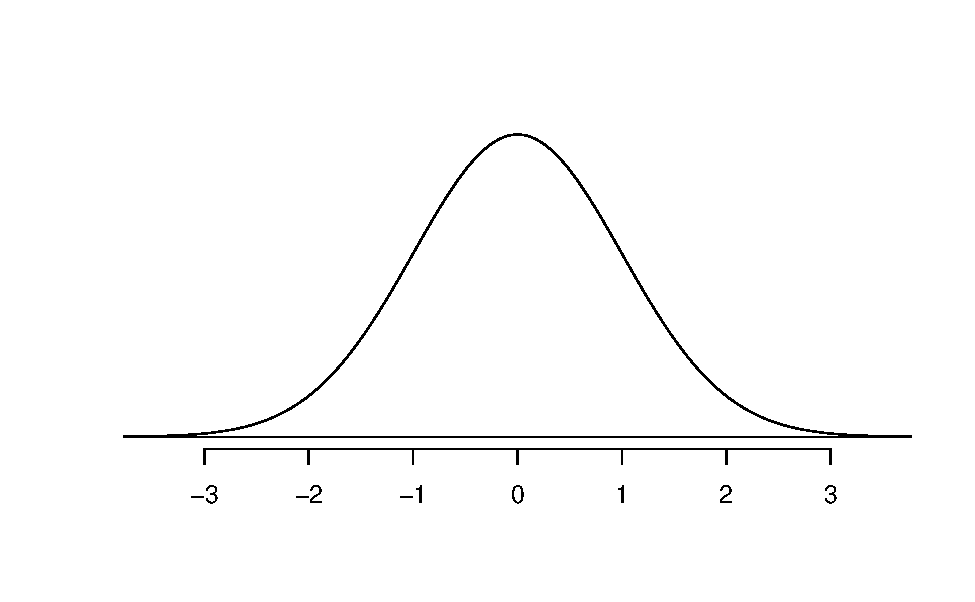
\includegraphics[width=0.5\linewidth]{04-A09-inference-1cat-theory_files/figure-latex/Norcuv-1} 

}

\caption{Standard Normal Curve}\label{fig:Norcuv}
\end{figure}

\begin{enumerate}
\def\labelenumi{\arabic{enumi}.}
\setcounter{enumi}{19}
\tightlist
\item
  How does a statistic closer to the null value affect the p-value?
\end{enumerate}

\vspace{0.3in}

\begin{enumerate}
\def\labelenumi{\arabic{enumi}.}
\setcounter{enumi}{20}
\tightlist
\item
  Summarize how each of the following affected the p-value:
\end{enumerate}

\begin{enumerate}
\def\labelenumi{\alph{enumi})}
\tightlist
\item
  Switching to a two-sided test.
\end{enumerate}

\vspace{0.4in}

\begin{enumerate}
\def\labelenumi{\alph{enumi})}
\setcounter{enumi}{1}
\tightlist
\item
  Using a smaller sample size.
\end{enumerate}

\vspace{0.4in}

\begin{enumerate}
\def\labelenumi{\alph{enumi})}
\setcounter{enumi}{2}
\tightlist
\item
  Using a sample statistic closer to the null value.
\end{enumerate}

\vspace{0.4in}

\subsection{Take-home messages}\label{take-home-messages-8}

\begin{enumerate}
\def\labelenumi{\arabic{enumi}.}
\item
  Both simulation and theory-based methods can be used to find a p-value for a hypothesis test. In order to use theory-based methods we need to check that both the independence and the success-failure conditions are met.
\item
  The standardized statistic measures how many standard errors the statistic is from the null value. The larger the standardized statistic the more evidence there is against the null hypothesis.
\item
  The p-value for a two-sided test is approximately two times the value for a one-sided test. A two-sided test provides less evidence against the null hypothesis.
\item
  The larger the sample size, the smaller the sample to sample variability. This will result in a larger standardized statistic and more evidence against the null hypothesis.
\item
  The farther the statistic is from the null value, the larger the standardized statistic. This will result in a smaller p-value and more evidence against the null hypothesis.
\end{enumerate}

\subsection{Additional notes}\label{additional-notes-8}

Use this space to summarize your thoughts and take additional notes on today's activity and material covered.

\newpage

\section{Activity 10: Confidence interval and what confidence means}\label{activity-10-confidence-interval-and-what-confidence-means}

\setstretch{1}

\subsection{Learning outcomes}\label{learning-outcomes-9}

\begin{itemize}
\item
  Explore what confidence means
\item
  Interpret the confidence level
\item
  Explore impact of sample size, direction of the alternative hypothesis, and value of the sample statistic on the p-value.
\end{itemize}

\subsection{Terminology review}\label{terminology-review-8}

In this activity, we will explore what being 95\% confidence means. Some terms covered in this activity are:

\begin{itemize}
\item
  Parameter of interest
\item
  Two-sided vs.~one-sided tests
\item
  Confidence level
\end{itemize}

\subsection{Handedness of male boxers continued}\label{handedness-of-male-boxers-continued}

In today's activity, we will use the male boxer study to look at what confidence means.

Left-handedness is a trait that is found in about 10\% of the general population. Past studies have shown that left-handed men are over-represented among professional boxers (Richardson and Gilman 2019). The fighting claim states that left-handed men have an advantage in competition. In this random sample of 500 male professional boxers, we want to see if there is an over-prevalence of left-handed fighters. In the sample of 500 male boxers, 81 were left-handed.

\begin{Shaded}
\begin{Highlighting}[]
 \CommentTok{\# Read in data set}
\NormalTok{boxers }\OtherTok{\textless{}{-}} \FunctionTok{read.csv}\NormalTok{(}\StringTok{"https://math.montana.edu/courses/s216/data/Male\_boxers\_sample.csv"}\NormalTok{)}
\NormalTok{boxers }\SpecialCharTok{\%\textgreater{}\%} \FunctionTok{count}\NormalTok{(Stance)  }\CommentTok{\# Count number in each Stance category}
\end{Highlighting}
\end{Shaded}

\begin{verbatim}
#>         Stance   n
#> 1  left-handed  81
#> 2 right-handed 419
\end{verbatim}

\subsection*{\texorpdfstring{What does \emph{confidence} mean?}{What does confidence mean?}}\label{what-does-confidence-mean}
\addcontentsline{toc}{subsection}{What does \emph{confidence} mean?}

In the interpretation of a 95\% confidence interval, we say that we are 95\% confident that the parameter is within the confidence interval. Why are we able to make that claim? What does it mean to say ``we are 95\% confident''?

\begin{enumerate}
\def\labelenumi{\arabic{enumi}.}
\tightlist
\item
  In the last activity we found very strong evidence that the true proportion of male professional boxers that are left-handed is greater than 0.1. As a class, determine a plausible value for the true proportion of male boxers that are left-handed. \emph{Note: we are making assumptions about the population here. This is not based on our calculated data, but we will use this applet to better understand what happens when we take many, many samples from this believed population.}
\end{enumerate}

\vspace{0.2in}

\begin{enumerate}
\def\labelenumi{\arabic{enumi}.}
\setcounter{enumi}{1}
\tightlist
\item
  Go to this website, \url{http://www.rossmanchance.com/ISIapplets.html} and choose `Simulating Confidence Intervals'. In the input on the left-hand side of the screen enter the value from question 1 for \(\pi\) (the true value), 500 for \(n\), and 100 for `Number of intervals'. Click `sample'.
\end{enumerate}

\vspace{1mm}

\begin{itemize}
\tightlist
\item
  In the graph on the bottom right, click on a green dot. Write down the confidence interval for this sample given on the graph on the left. Does this confidence interval contain the true value chosen in question 1?
\end{itemize}

\vspace{0.4in}

\begin{itemize}
\item
  Now click on a red dot. Write down the confidence interval for this sample. Does this confidence interval contain the true value chosen in question 1?
  \vspace{0.5in}
\item
  How many intervals out of 100 contain \(\pi\), the true value chosen in question 1? \emph{Hint}: This is given to the left of the graph of green and red intervals.
  \vspace{0.4in}
\end{itemize}

\begin{enumerate}
\def\labelenumi{\arabic{enumi}.}
\setcounter{enumi}{2}
\tightlist
\item
  Click on `sample' nine more times. Write down the `Running Total' for the proportion of intervals that contain \(\pi\).
\end{enumerate}

\vspace{0.5in}

\begin{enumerate}
\def\labelenumi{\arabic{enumi}.}
\setcounter{enumi}{3}
\tightlist
\item
  Change the confidence level to 90\%. What happened to the width of the intervals?
\end{enumerate}

\vspace{0.2in}

\begin{enumerate}
\def\labelenumi{\arabic{enumi}.}
\setcounter{enumi}{4}
\tightlist
\item
  Write down the \texttt{Running\ Total} for the proportion of intervals that contain \(\pi\) using a 90\% confidence level.
\end{enumerate}

\vspace{0.4in}

\begin{enumerate}
\def\labelenumi{\arabic{enumi}.}
\setcounter{enumi}{5}
\tightlist
\item
  Interpret the level of confidence. \emph{Hint}: What proportion of samples would we expect to give a confidence interval that contains the parameter of interest?
\end{enumerate}

\vspace{0.8in}

\subsubsection*{Theory-based confidence interval}\label{theory-based-confidence-interval}
\addcontentsline{toc}{subsubsection}{Theory-based confidence interval}

To calculate a theory-based 95\% confidence interval for \(\pi\), we will first find the \textbf{standard error} of \(\hat{p}\) by plugging in the value of \(\hat{p}\) for \(\pi\) in \(SD(\hat{p})\):

\[SE(\hat{p}) = \sqrt{\frac{\hat{p}\times (1-\hat{p})}{n}}\]

Note that we do not include a ``0'' subscript, since we are not assuming a null hypothesis.

\begin{enumerate}
\def\labelenumi{\arabic{enumi}.}
\setcounter{enumi}{6}
\tightlist
\item
  Calculate the standard error of the sample proportion to find a 95\% confidence interval.
\end{enumerate}

\vspace{0.5in}

We will calculate the margin of error and confidence interval in questions 10 and 11 of this activity. \textbf{The margin of error (ME)} is the value of the \(z^*\) multiplier times the standard error of the statistic.

\[ME = z^* \times SE(\hat{p})\]
The \(z^*\) multiplier is the percentile of a standard normal distribution that corresponds to our confidence level. If our confidence level is 95\%, we find the Z values that encompass the middle 95\% of the standard normal distribution. If 95\% of the standard normal distribution should be in the middle, that leaves 5\% in the tails, or 2.5\% in each tail.

The \texttt{qnorm()} function in R will tell us the \(z^*\) value for the desired percentile (in this case, 95\% + 2.5\% = 97.5\% percentile).

\begin{itemize}
\item
  Enter the value of 0.975 for xx in the provided R script file.
\item
  Highlight and run line 12. This will give the value of the multiplier for a 95\% confidence interval.
\end{itemize}

\begin{Shaded}
\begin{Highlighting}[]
\FunctionTok{qnorm}\NormalTok{(xx, }\AttributeTok{lower.tail =} \ConstantTok{TRUE}\NormalTok{) }\CommentTok{\# Multiplier for 95\% confidence interval}
\end{Highlighting}
\end{Shaded}

\begin{enumerate}
\def\labelenumi{\arabic{enumi}.}
\setcounter{enumi}{7}
\item
  Report the value of the multiplier needed to calculate the 95\% confidence interval for the true proportion of male boxers that are left-handed.
  \vspace{0.2in}
\item
  Fill in the normal distribution shown below to show how R found the \(z^*\) multiplier.
\end{enumerate}

\begin{figure}

{\centering 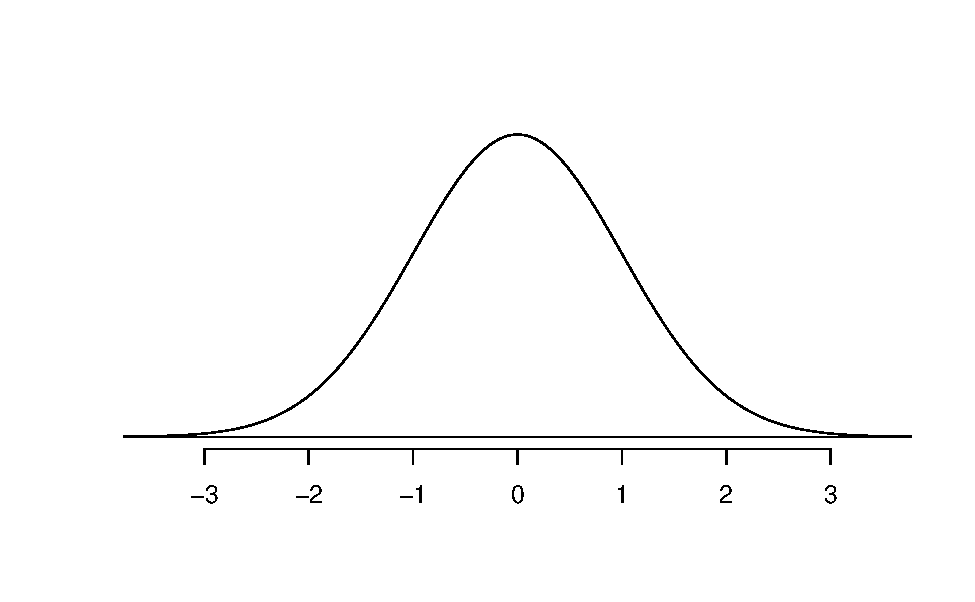
\includegraphics[width=0.45\linewidth]{04-A10-confidenceLevel_files/figure-latex/Normalcur-1} 

}

\caption{Standard Normal Curve}\label{fig:Normalcur}
\end{figure}

\begin{enumerate}
\def\labelenumi{\arabic{enumi}.}
\setcounter{enumi}{9}
\tightlist
\item
  Calculate the margin of error for the 95\% confidence interval.
  \vspace{0.6in}
\end{enumerate}

To find the confidence interval, we will add and subtract the \textbf{margin of error} to the point estimate:
\[\text{point estimate}\pm\text{margin of error}\]
\[\hat{p}\pm z^* \times SE(\hat{p})\]

\begin{enumerate}
\def\labelenumi{\arabic{enumi}.}
\setcounter{enumi}{10}
\item
  Calculate the 95\% confidence interval for the parameter of interest.
  \vspace{0.6in}
\item
  Interpret the 95\% confidence \textbf{interval} in the context of the problem.
  \vspace{1in}
\end{enumerate}

\subsection{Take-home messages}\label{take-home-messages-9}

\begin{enumerate}
\def\labelenumi{\arabic{enumi}.}
\item
  If repeat samples of the same size are selected from the population, approximately 95\% of samples will create a 95\% confidence interval that contains the parameter of interest.
\item
  The calculation of the confidence interval uses the standard error calculated using the sample proportion rather than the null value.
\end{enumerate}

\subsection{Additional notes}\label{additional-notes-9}

Use this space to summarize your thoughts and take additional notes on today's activity and material covered.

\newpage

\section{Module 3 and 4 Lab: Mixed Breed Dogs in the U.S.}\label{module-3-and-4-lab-mixed-breed-dogs-in-the-u.s.}

\setstretch{1}

\subsection{Learning outcomes}\label{learning-outcomes-10}

\begin{itemize}
\item
  Determine whether simulation or theory-based methods of inference can be used.
\item
  Analyze and interpret a study involving a single categorical variable.
\end{itemize}

\subsection{Mixed Breed Dogs in the U.S.}\label{mixed-breed-dogs-in-the-u.s.}

The American Veterinary Medical Association estimated in 2010 that approximately 49\% of dog owners in the U.S. own dogs that are classified as ``mixed breed.'' As part of a larger 2022 international study (Banton 2022) about overall dog health, survey participants were asked, among other things, to report whether their dog was purebred or a mixed breed. Seven hundred and fifty (750) dog owners from the U.S. were recruited to complete an online survey via an email indicating they had been randomly selected by Qualtrics (an ``experience management'' company that specializes in surveys). Three hundred sixty-four (364) out of 675 respondents from the U.S. reported they owned a mixed breed dog. Is there evidence that, in the last decade, the proportion of dog owners in the U.S. that own a mixed breed dog has changed from the value reported in 2010?

\subsubsection*{Activity intro}\label{activity-intro-1}
\addcontentsline{toc}{subsubsection}{Activity intro}

\begin{itemize}
\item
  Download the R script file and the data file (US\_dogs.csv) from D2L
\item
  Upload both files to D2L and open the R script file
\item
  Enter the name of the dataset for datasetname.csv.
\item
  Highlight and run lines 1 - 6
\end{itemize}

\begin{enumerate}
\def\labelenumi{\arabic{enumi}.}
\tightlist
\item
  What is the value of the point estimate?
\end{enumerate}

\vspace{0.3in}

\begin{enumerate}
\def\labelenumi{\arabic{enumi}.}
\setcounter{enumi}{1}
\tightlist
\item
  Create a plot of the data using the R code. Make sure to include an appropriate title with type of plot, observational units, and variable. \textbf{Upload the plot to Gradescope}.
\end{enumerate}

\begin{Shaded}
\begin{Highlighting}[]
\NormalTok{dogs }\SpecialCharTok{\%\textgreater{}\%} \CommentTok{\# Data set piped into...}
    \FunctionTok{ggplot}\NormalTok{(}\FunctionTok{aes}\NormalTok{(}\AttributeTok{x =}\NormalTok{ variable)) }\SpecialCharTok{+}   \CommentTok{\# This specifies the variable}
    \FunctionTok{geom\_bar}\NormalTok{(}\FunctionTok{aes}\NormalTok{(}\AttributeTok{y =} \FunctionTok{after\_stat}\NormalTok{(prop), }\AttributeTok{group =} \DecValTok{1}\NormalTok{)) }\SpecialCharTok{+}  \CommentTok{\# Tell it to make a bar plot with proportions}
    \FunctionTok{labs}\NormalTok{(}\AttributeTok{title =} \StringTok{"Don\textquotesingle{}t forget to title your plot"}\NormalTok{,  }
       \CommentTok{\# Give your plot a title}
       \AttributeTok{x =} \StringTok{"Breed of Dog"}\NormalTok{,   }\CommentTok{\# Label the x axis}
       \AttributeTok{y =} \StringTok{"Relative Frequency"}\NormalTok{)  }\CommentTok{\# Label the y axis}
\end{Highlighting}
\end{Shaded}

\subsubsection*{Use statistical analysis methods to draw inferences from the data}\label{use-statistical-analysis-methods-to-draw-inferences-from-the-data-2}
\addcontentsline{toc}{subsubsection}{Use statistical analysis methods to draw inferences from the data}

\begin{enumerate}
\def\labelenumi{\arabic{enumi}.}
\setcounter{enumi}{2}
\tightlist
\item
  \textbf{Write out the parameter of interest in words, in context of the study.}
\end{enumerate}

\vspace{0.5in}

\begin{enumerate}
\def\labelenumi{\arabic{enumi}.}
\setcounter{enumi}{3}
\tightlist
\item
  Write out the null and alternative hypotheses in notation.
\end{enumerate}

\vspace{1mm}

\(H_0:\)

\vspace{0.3in}

\(H_A:\)

\vspace{0.3in}

\begin{enumerate}
\def\labelenumi{\arabic{enumi}.}
\setcounter{enumi}{4}
\tightlist
\item
  \textbf{Will theory-based methods give the same results as simulation based methods? Explain your answer.}
\end{enumerate}

\vspace{1in}

To use the computer simulation, we will need to enter the

\begin{itemize}
\item
  assumed ``probability of success'' (\(\pi_0\)),
\item
  ``sample size'' (the number of observational units or cases in the sample),
\item
  ``number of repetitions'' (the number of samples to be generated),
\item
  ``as extreme as'' (the observed statistic), and
\item
  the ``direction'' (matches the direction of the alternative hypothesis).
\end{itemize}

We will use the \texttt{one\_proportion\_test()} function in \texttt{R} (in the \texttt{catstats} package) to simulate the null distribution of sample proportions and compute a p-value.

\begin{itemize}
\item
  Using the provided \texttt{R} script file, fill in the values/words for each \texttt{xx} in the one proportion test to create a null distribution with 10000 simulations.
\item
  Then highlight and run lines 21--26.
\end{itemize}

\begin{Shaded}
\begin{Highlighting}[]
\FunctionTok{one\_proportion\_test}\NormalTok{(}\AttributeTok{probability\_success =}\NormalTok{ xx, }\CommentTok{\# Null hypothesis value}
          \AttributeTok{sample\_size =}\NormalTok{ xx, }\CommentTok{\# Enter sample size}
          \AttributeTok{number\_repetitions =} \DecValTok{10000}\NormalTok{, }\CommentTok{\# Enter number of simulations}
          \AttributeTok{as\_extreme\_as =}\NormalTok{ xx, }\CommentTok{\# Observed statistic}
          \AttributeTok{direction =} \StringTok{"xx"}\NormalTok{, }\CommentTok{\# Specify direction of alternative hypothesis}
          \AttributeTok{summary\_measure =} \StringTok{"proportion"}\NormalTok{) }\CommentTok{\# Reporting proportion or number of successes?}
\end{Highlighting}
\end{Shaded}

\begin{enumerate}
\def\labelenumi{\arabic{enumi}.}
\setcounter{enumi}{5}
\tightlist
\item
  Report the p-value from the study.
\end{enumerate}

\vspace{0.2in}

The \(z^*\) multiplier is the percentile of a standard normal distribution that corresponds to our confidence level.

\begin{itemize}
\item
  Enter the value of the appropriate percentile in the provided R script file to find the multiplier for a 90\% confidence interval.
\item
  Highlight and run line 31
\end{itemize}

\begin{Shaded}
\begin{Highlighting}[]
\FunctionTok{qnorm}\NormalTok{(percentile, }\AttributeTok{lower.tail =} \ConstantTok{TRUE}\NormalTok{) }\CommentTok{\# Multiplier for 90\% confidence interval}
\end{Highlighting}
\end{Shaded}

\begin{enumerate}
\def\labelenumi{\arabic{enumi}.}
\setcounter{enumi}{6}
\tightlist
\item
  \textbf{Calculate the margin of error for a 90\% confidence interval.}
\end{enumerate}

\vspace{0.6in}

\begin{enumerate}
\def\labelenumi{\arabic{enumi}.}
\setcounter{enumi}{7}
\tightlist
\item
  Calculate a 90\% confidence interval.
\end{enumerate}

\vspace{0.6in}

\newpage

\subsubsection*{Summarize the results of the study}\label{summarize-the-results-of-the-study}
\addcontentsline{toc}{subsubsection}{Summarize the results of the study}

\begin{enumerate}
\def\labelenumi{\arabic{enumi}.}
\setcounter{enumi}{8}
\tightlist
\item
  Write a paragraph summarizing the results of the study. Be sure to describe:
\end{enumerate}

\begin{itemize}
\item
  Summary statistic and interpretation

  \begin{itemize}
  \item
    Summary measure (in context)
  \item
    Value of the statistic
  \item
    Order of subtraction when comparing two groups
  \end{itemize}
\item
  P-value and interpretation

  \begin{itemize}
  \item
    Statement about probability or proportion of samples
  \item
    Statistic (summary measure and value)
  \item
    Direction of the alternative
  \item
    Null hypothesis (in context)
  \end{itemize}
\item
  Confidence interval and interpretation

  \begin{itemize}
  \item
    How confident you are (e.g., 90\%, 95\%, 98\%, 99\%)
  \item
    Parameter of interest
  \item
    Calculated interval
  \item
    Order of subtraction when comparing two groups
  \end{itemize}
\item
  Conclusion (written to answer the research question)

  \begin{itemize}
  \item
    Amount of evidence
  \item
    Parameter of interest
  \item
    Direction of the alternative hypothesis
  \end{itemize}
\item
  Scope of inference

  \begin{itemize}
  \item
    To what group of observational units do the results apply (target population or observational units similar to the sample)?
  \item
    What type of inference is appropriate (causal or non-causal)?
  \end{itemize}
\end{itemize}

\textbf{Upload a copy of your group's paragraph to Gradescope.}

\newpage

Paragraph (continued):

\newpage

\chapter{Unit 1 Review}\label{unit-1-review}

The following module contains both a list of key topics covered in Unit 1 as well as Module Review Worksheets that will be covered in Weekly Review Sessions.

\subsection{Key Topics}\label{key-topics-4}

Review the key topics for Unit 1 prior to the first exams. All of these topics will be covered in Modules 1--4.

\subsection{Module Review}\label{module-review}

\setstretch{1}

The following worksheets review each of the modules. These worksheets will be completed during Melinda's Study Sessions each week. Solutions will be posted on D2L in the Unit 1 Review folder after the study sessions.

\newpage

\section{Key Topics Exam 1}\label{key-topics-exam-1}

\subsection*{Descriptive statistics and study design}\label{descriptive-statistics-and-study-design}
\addcontentsline{toc}{subsection}{Descriptive statistics and study design}

\begin{enumerate}
\def\labelenumi{\arabic{enumi}.}
\item
  Identify the observational units.
\item
  Identify the types of variables (categorical or quantitative).
\item
  Identify the explanatory variable (if present) and the response variable (roles of variables).
\item
  Identify the appropriate type of graph and summary measure.
\item
  Identify if a given value is a statistic or a parameter. Identify the appropriate notation.
\item
  Identify the study design (observational study or randomized experiment).
\item
  Identify the sampling method and potential types of sampling bias (non-response, response, selection).
\item
  Identify and interpret the summary statistic
\item
  Identify the target population
\item
  Identify the types of sampling bias (response, non-response, selection, none)
\item
  Identify the type(s) of graph(s) that could be used to plot the given variable(s).
\end{enumerate}

\subsection*{Hypothesis testing}\label{hypothesis-testing-1}
\addcontentsline{toc}{subsection}{Hypothesis testing}

\begin{enumerate}
\def\labelenumi{\arabic{enumi}.}
\setcounter{enumi}{11}
\item
  Write the parameter of interest in context of the problem.
\item
  State the null and alternative hypotheses in both words and notation
\item
  Verify the validity condition is met to use simulation-based methods to find a p-value.
\item
  Verify the validity conditions are met to use theory-based methods to find a p-value from the theoretical distribution.
\item
  In a simulation-based hypothesis test, describe how to create one dot on a dotplot of the null distribution using coins, cards, or spinners.
\item
  Explain where the null distribution is centered and why.
\item
  Describe and illustrate how R calculates the p-value for a simulation-based test.
\item
  Describe and illustrate how R calculates the p-value for a theory-based test.
\item
  Type of theoretical distribution (standard normal distribution or t-distribution with appropriate degrees of freedom) used to model the standardized statistic in a theory-based hypothesis test.
\item
  Calculate and interpret the standard error of the statistic under the null using the correct formula on the Golden ticket.
\item
  Calculate and interpret the appropriate standardized statistic using the correct formula on the Golden ticket.
\item
  Interpret the p-value in context of the study: it is the probability of \_\_\_\_, assuming \_\_\_\_.
\item
  Evaluate the p-value for strength of evidence against the null: how much evidence does the p-value provide against the null?
\item
  Write a conclusion about the research question based on the p-value.
\item
  Describe which features of the study impact the p-value and how.
\end{enumerate}

\subsection{Confidence intervals}\label{confidence-intervals}

\begin{enumerate}
\def\labelenumi{\arabic{enumi}.}
\setcounter{enumi}{26}
\item
  Describe how to simulate one bootstrapped sample using cards.
\item
  Explain where the bootstrap distribution is centered and why.
\item
  Find an appropriate percentile confidence interval using a bootstrap distribution from R output.
\item
  Verify the validity condition is met to use simulation-based methods to find the confidence interval.
\item
  Verify the validity conditions are met to use theory-based methods to calculate a confidence interval.
\item
  Describe and illustrate how the bootstrap distribution is used to find the confidence interval for a given confidence level.
\item
  Describe and illustrate how the standard normal distribution or t-distribution is used to find the multiplier for a given confidence level.
\item
  Calculate and interpret the standard error of the statistic (not assuming the null hypothesis) using the correct formula on the Golden ticket
\item
  Calculate the appropriate margin of error and confidence interval using theory-based methods.
\item
  Interpret the confidence interval in context of the study.
\item
  Based on the interval, what decision can you make about the null hypothesis? Does the confidence interval agree with the results of the hypothesis test? Justify your answer.
\item
  Interpret the confidence level in context of the study. What does ``confidence'' mean?
\item
  Describe which features of the study have an effect on the width of the confidence interval and how.
\end{enumerate}

\subsection{Probability}\label{probability-3}

\begin{enumerate}
\def\labelenumi{\arabic{enumi}.}
\setcounter{enumi}{39}
\item
  Calculate probabilities from a given table and give appropriate probability notation for both conditional and unconditional probabilities.
\item
  Create a two-way table using given probabilities.
\item
  Interpret a probability value in context of the problem.
\end{enumerate}

\newpage

\section{Module 1 Review - Sampling Methods}\label{module-1-review---sampling-methods}

\begin{enumerate}
\def\labelenumi{\arabic{enumi}.}
\tightlist
\item
  Suppose that the proportion of all American adults that fit the medical definition of being obese is 0.23. A large medical clinic would like to determine if the proportion of their patients that are obese is higher than that of all American adults. The clinic takes a simple random sample of 30 of their patients and finds that 9 patients in the sample are obese.
\end{enumerate}

\begin{enumerate}
\def\labelenumi{\alph{enumi}.}
\tightlist
\item
  What is the target population?
\end{enumerate}

\vspace{0.4in}

\begin{enumerate}
\def\labelenumi{\alph{enumi}.}
\setcounter{enumi}{1}
\tightlist
\item
  What are the observational units?
\end{enumerate}

\vspace{0.4in}

\begin{enumerate}
\def\labelenumi{\alph{enumi}.}
\setcounter{enumi}{2}
\tightlist
\item
  What variable is being studied?
\end{enumerate}

\vspace{0.4in}

\begin{enumerate}
\def\labelenumi{\alph{enumi}.}
\setcounter{enumi}{3}
\tightlist
\item
  Is the variable identified in part (c) categorical or quantitative?
\end{enumerate}

\vspace{0.4in}

\begin{enumerate}
\def\labelenumi{\arabic{enumi}.}
\setcounter{enumi}{1}
\tightlist
\item
  Martha works in Macy's advertising department. She is interested in the shopping experience of all Macy's shoppers in the U.S. Every Saturday morning for a month she stands outside of the Bozeman Macy's asking people about their experience. One of the questions she uses is: ``As a huge fan of Macy's, I believe Macy's has the best choices of clothing in Bozeman. Don't you agree?'' Every person that was asked, responded.
\end{enumerate}

\begin{enumerate}
\def\labelenumi{\alph{enumi}.}
\tightlist
\item
  Identify the target population.
\end{enumerate}

\vspace{0.4in}

\begin{enumerate}
\def\labelenumi{\alph{enumi}.}
\setcounter{enumi}{1}
\tightlist
\item
  Identify the sample.
\end{enumerate}

\vspace{0.4in}

\begin{enumerate}
\def\labelenumi{\alph{enumi}.}
\setcounter{enumi}{2}
\tightlist
\item
  Which of the three types of sampling bias (selection, non-response, response) may be present? Explain your choice(s).
\end{enumerate}

\vspace{0.5in}

\newpage

\begin{enumerate}
\def\labelenumi{\arabic{enumi}.}
\setcounter{enumi}{2}
\tightlist
\item
  This study aims to explore whether Swiss university students feeling academic study pressure (whether the student had experienced academic failure) tend to use psychotropic drugs (whether the student had used psychotropic drugs during the student's time at university) as a coping mechanism. An invitation email was sent to all bachelor's and master's students at the University of Lausanne, totaling 15,400 individuals, with a link to access the online questionnaire containing 49 questions and 107 items. No reminder was sent out, and no incentive was given to complete the questionnaire. A total of 1,690 students initially participated in the study, but 424 questionnaires were too incomplete to be used for analysis and were excluded. Additionally, 67 questionnaires were removed because of significant missing sociodemographic information, resulting in 1,199 completed responses included in the final analysis. Is there an association between study pressure and use of psychotropic drugs among Swiss University students?
\end{enumerate}

\begin{enumerate}
\def\labelenumi{\alph{enumi}.}
\tightlist
\item
  Identify the target population.
\end{enumerate}

\vspace{0.4in}

\begin{enumerate}
\def\labelenumi{\alph{enumi}.}
\setcounter{enumi}{1}
\tightlist
\item
  Identify the sample.
\end{enumerate}

\vspace{0.4in}

\begin{enumerate}
\def\labelenumi{\alph{enumi}.}
\setcounter{enumi}{2}
\tightlist
\item
  Which of the three types of sampling bias (selection, non-response, response) may be present? Explain your choice(s).
\end{enumerate}

\vspace{0.4in}

\begin{enumerate}
\def\labelenumi{\alph{enumi}.}
\setcounter{enumi}{3}
\tightlist
\item
  Identify the type and roles of each variable in the study.
\end{enumerate}

\vspace{0.6in}

\begin{enumerate}
\def\labelenumi{\arabic{enumi}.}
\setcounter{enumi}{3}
\tightlist
\item
  Researchers decided to investigate whether a cat's coat color is associated with aggressive cat behavior by creating a 20-minute survey. The survey was distributed by posting it to social media and through cat-related listservs (e.g., For the Love of Cats), inviting individuals to take the survey. A total of 1,365 surveys were completed by participants. The frequency of each of the following aggressive behavior categories was assessed: hiss, stalk/chase, bite, slap/scratch. Frequency of behaviors toward people were recorded on a 6-point scale: 0 = never, 1 = less than once every 6 months, 2 = once every 6 months, 3 = once per month, 4 = once per week, 5 = one or more times per day. Because there were four aggressive behavior categories, each with a frequency of 0 to 5 possible, each cat could score between 0 to 20 for human aggression. Is there an association between coat color and aggressive behavior among cats?
\end{enumerate}

\begin{enumerate}
\def\labelenumi{\alph{enumi}.}
\tightlist
\item
  Identify the target population.
\end{enumerate}

\vspace{0.4in}

\begin{enumerate}
\def\labelenumi{\alph{enumi}.}
\setcounter{enumi}{1}
\tightlist
\item
  Identify the sample.
\end{enumerate}

\vspace{0.4in}

\begin{enumerate}
\def\labelenumi{\alph{enumi}.}
\setcounter{enumi}{2}
\tightlist
\item
  Which of the three types of sampling bias (selection, non-response, response) may be present? Explain your choice(s).
\end{enumerate}

\vspace{0.4in}

\begin{enumerate}
\def\labelenumi{\alph{enumi}.}
\setcounter{enumi}{3}
\tightlist
\item
  Identify the type and roles of each variable in the study.
\end{enumerate}

\vspace{0.6in}

\newpage

\section{Module 2 Review - Probability}\label{module-2-review---probability}

\begin{enumerate}
\def\labelenumi{\arabic{enumi}.}
\tightlist
\item
  Spelling errors in a text can either be non-word errors (teh instead of the) or word errors (lose instead of loose). It was found that non-word errors make up about 25\% of all errors. A human proofreader will catch 92\% of non-word errors and 75\% of word errors.
\end{enumerate}

Let N represent non-word errors and C represent that a human proofreader will catch the error.

\begin{enumerate}
\def\labelenumi{\alph{enumi}.}
\item
  Identify the following values with appropriate probability notation.
  \vspace{2mm}

  \(0.25\)
  \vspace{2mm}

  \(0.92\)
  \vspace{2mm}

  \(0.75\)
  \vspace{2mm}
\item
  Fill in the table below to represent the situation:
\end{enumerate}

\begin{center}
\begin{tabular}{|c|c|c|c|} \hline
\hspace{0.8in} & \hspace{0.25in}  $N$ \hspace{.25in} & \hspace{0.25in} $N^C$ \hspace{0.25in} & \hspace{0.25in} Total \hspace{0.25in} \\ \hline
 $C$ &  &  &  \\ \hline
 $C^C$ &  & &  \\ \hline
Total &  &  & 100000 \\ \hline
\end{tabular}
\end{center}
\vspace{.1in}

\begin{enumerate}
\def\labelenumi{\alph{enumi}.}
\setcounter{enumi}{2}
\tightlist
\item
  Using your table calculate the probability that a randomly selected error caught by a human proofreader is a non-word error. Use appropriate probability notation.
\end{enumerate}

\vspace{1in}

\begin{enumerate}
\def\labelenumi{\alph{enumi}.}
\setcounter{enumi}{3}
\tightlist
\item
  Find the probability a selected error is a non-word error and was not caught by a human proofreader. Use appropriate probability notation.
\end{enumerate}

\vspace{1in}

\begin{enumerate}
\def\labelenumi{\alph{enumi}.}
\setcounter{enumi}{4}
\tightlist
\item
  Find the value of \(P(N|C)\). What does this probability mean?
\end{enumerate}

\vspace{1in}

\newpage

\begin{enumerate}
\def\labelenumi{\arabic{enumi}.}
\setcounter{enumi}{1}
\tightlist
\item
  A private college report contains these statistics:
\end{enumerate}

\begin{itemize}
\item
  70\% of incoming freshmen attended public schools
\item
  75\% of public-school students who enroll as freshmen eventually graduate
\item
  90\% of other freshmen eventually graduate
\end{itemize}

Let A represent the event that a freshman attended public school and B the event that a freshman eventually graduates.

\begin{enumerate}
\def\labelenumi{\alph{enumi}.}
\item
  Identify the following values with appropriate probability notation.
  \vspace{2mm}

  \(0.70\)
  \vspace{2mm}

  \(0.75\)
  \vspace{2mm}

  \(0.90\)
  \vspace{2mm}
\item
  Fill in the table below to represent the situation:
\end{enumerate}

\begin{center}
\begin{tabular}{|c|c|c|c|} \hline
\hspace{0.8in} & \hspace{0.25in}  $A$ \hspace{.25in} & \hspace{0.25in} $A^C$ \hspace{0.25in} & \hspace{0.25in} Total \hspace{0.25in} \\ \hline
 $B$ &  &  &  \\ \hline
 $B^C$ &  & &  \\ \hline
Total &  &  & 100000 \\ \hline
\end{tabular}
\end{center}
\vspace{.1in}

\begin{enumerate}
\def\labelenumi{\alph{enumi}.}
\setcounter{enumi}{2}
\tightlist
\item
  Calculate the probability a selected freshman attended public school given they did not graduate. Use appropriate probability notation.
\end{enumerate}

\vspace{1in}

\begin{enumerate}
\def\labelenumi{\alph{enumi}.}
\setcounter{enumi}{3}
\tightlist
\item
  Calculate the probability a selected freshman does not graduate. Use appropriate probability notation.
\end{enumerate}

\vspace{1in}

\begin{enumerate}
\def\labelenumi{\alph{enumi}.}
\setcounter{enumi}{4}
\tightlist
\item
  Of the population of freshman that attended public school, what is the probability they do not graduate. Use appropriate probability notation.
\end{enumerate}

\vspace{1in}

\begin{enumerate}
\def\labelenumi{\alph{enumi}.}
\setcounter{enumi}{5}
\tightlist
\item
  Find the value of \(P(A~\text{and}~B^C)\). Write this probability in context of the problem.
\end{enumerate}

\newpage

\section{Module 3 Review - Simulation Methods for a Single Proportion}\label{module-3-review---simulation-methods-for-a-single-proportion}

\begin{Shaded}
\begin{Highlighting}[]
\NormalTok{hearing }\OtherTok{\textless{}{-}} \FunctionTok{read.csv}\NormalTok{(}\StringTok{"data/hearing\_loss.csv"}\NormalTok{)}
\end{Highlighting}
\end{Shaded}

A recent study examined hearing loss data for 1753 U.S. teenagers. In this sample, 328 were found to have some level of hearing loss. News of this study spread quickly, with many news articles blaming the prevalence of hearing loss on the higher use of ear buds by teens. At MSNBC.com (8/17/2010), Carla Johnson summarized the study with the headline: ``1 in 5 U.S. teens has hearing loss, study says.'' Is this an appropriate or a misleading headline?

\begin{enumerate}
\def\labelenumi{\arabic{enumi}.}
\tightlist
\item
  Write the parameter of interest in context of the study.
\end{enumerate}

\vspace{0.8in}

\begin{enumerate}
\def\labelenumi{\arabic{enumi}.}
\setcounter{enumi}{1}
\tightlist
\item
  Write the null hypothesis in words and notation in context of the problem.
\end{enumerate}

\vspace{1in}

\begin{enumerate}
\def\labelenumi{\arabic{enumi}.}
\setcounter{enumi}{2}
\tightlist
\item
  Based on the research questions, choose the direction for the alternative hypothesis.
\end{enumerate}

\vspace{0.3in}

\begin{enumerate}
\def\labelenumi{\arabic{enumi}.}
\setcounter{enumi}{3}
\tightlist
\item
  Write the alternative hypothesis in words and notation in context of the problem.
\end{enumerate}

\vspace{1in}

\begin{enumerate}
\def\labelenumi{\arabic{enumi}.}
\setcounter{enumi}{4}
\tightlist
\item
  Calculate the summary statistic. Use proper notation.
\end{enumerate}

\vspace{0.3in}

\begin{enumerate}
\def\labelenumi{\arabic{enumi}.}
\setcounter{enumi}{5}
\tightlist
\item
  What values should be entered for each of the following into the one proportion test to create 10000 simulations?
\end{enumerate}

\begin{itemize}
\tightlist
\item
  Probability of success:
\end{itemize}

\vspace{0.2in}

\begin{itemize}
\tightlist
\item
  Sample size:
\end{itemize}

\vspace{0.2in}

\begin{itemize}
\tightlist
\item
  Number of repetitions:
\end{itemize}

\vspace{0.2in}

\begin{itemize}
\tightlist
\item
  As extreme as:
\end{itemize}

\vspace{0.2in}

\begin{itemize}
\tightlist
\item
  Direction (``greater'', ``less'', or ``two-sided''):
\end{itemize}

\vspace{0.2in}

\begin{Shaded}
\begin{Highlighting}[]
\FunctionTok{one\_proportion\_test}\NormalTok{(}\AttributeTok{probability\_success =} \FloatTok{0.2}\NormalTok{, }\CommentTok{\#Null hypothesis value}
                    \AttributeTok{sample\_size =} \DecValTok{1753}\NormalTok{, }\CommentTok{\#Enter sample size}
                    \AttributeTok{number\_repetitions =} \DecValTok{10000}\NormalTok{, }\CommentTok{\#Enter number of simulations}
                    \AttributeTok{as\_extreme\_as =} \FloatTok{0.187}\NormalTok{, }\CommentTok{\#observed statistic}
                    \AttributeTok{direction =} \StringTok{"two{-}sided"}\NormalTok{, }\CommentTok{\#specify direction of alternative hypothesis}
                    \AttributeTok{summary\_measure =} \StringTok{"proportion"}\NormalTok{) }\CommentTok{\#Reporting proportion or number of successes?}
\end{Highlighting}
\end{Shaded}

\begin{center}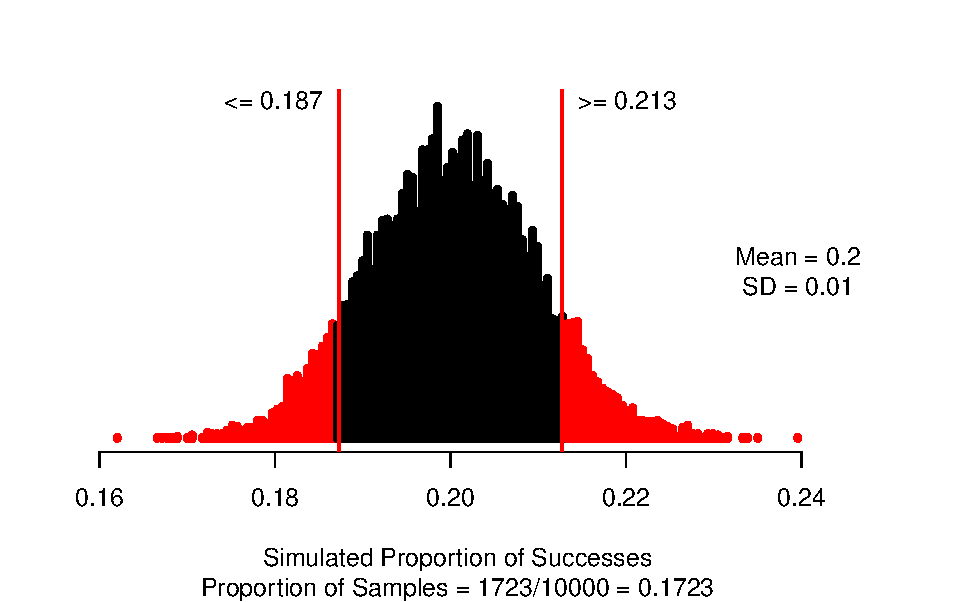
\includegraphics[width=0.7\linewidth]{05-UR-module3_review_files/figure-latex/unnamed-chunk-2-1} \end{center}

\begin{enumerate}
\def\labelenumi{\arabic{enumi}.}
\setcounter{enumi}{6}
\tightlist
\item
  Interpret the p-value in context of the problem.
\end{enumerate}

\vspace{1in}

\begin{enumerate}
\def\labelenumi{\arabic{enumi}.}
\setcounter{enumi}{7}
\tightlist
\item
  How much evidence does the data provide against the null hypothesis?
\end{enumerate}

\begin{center}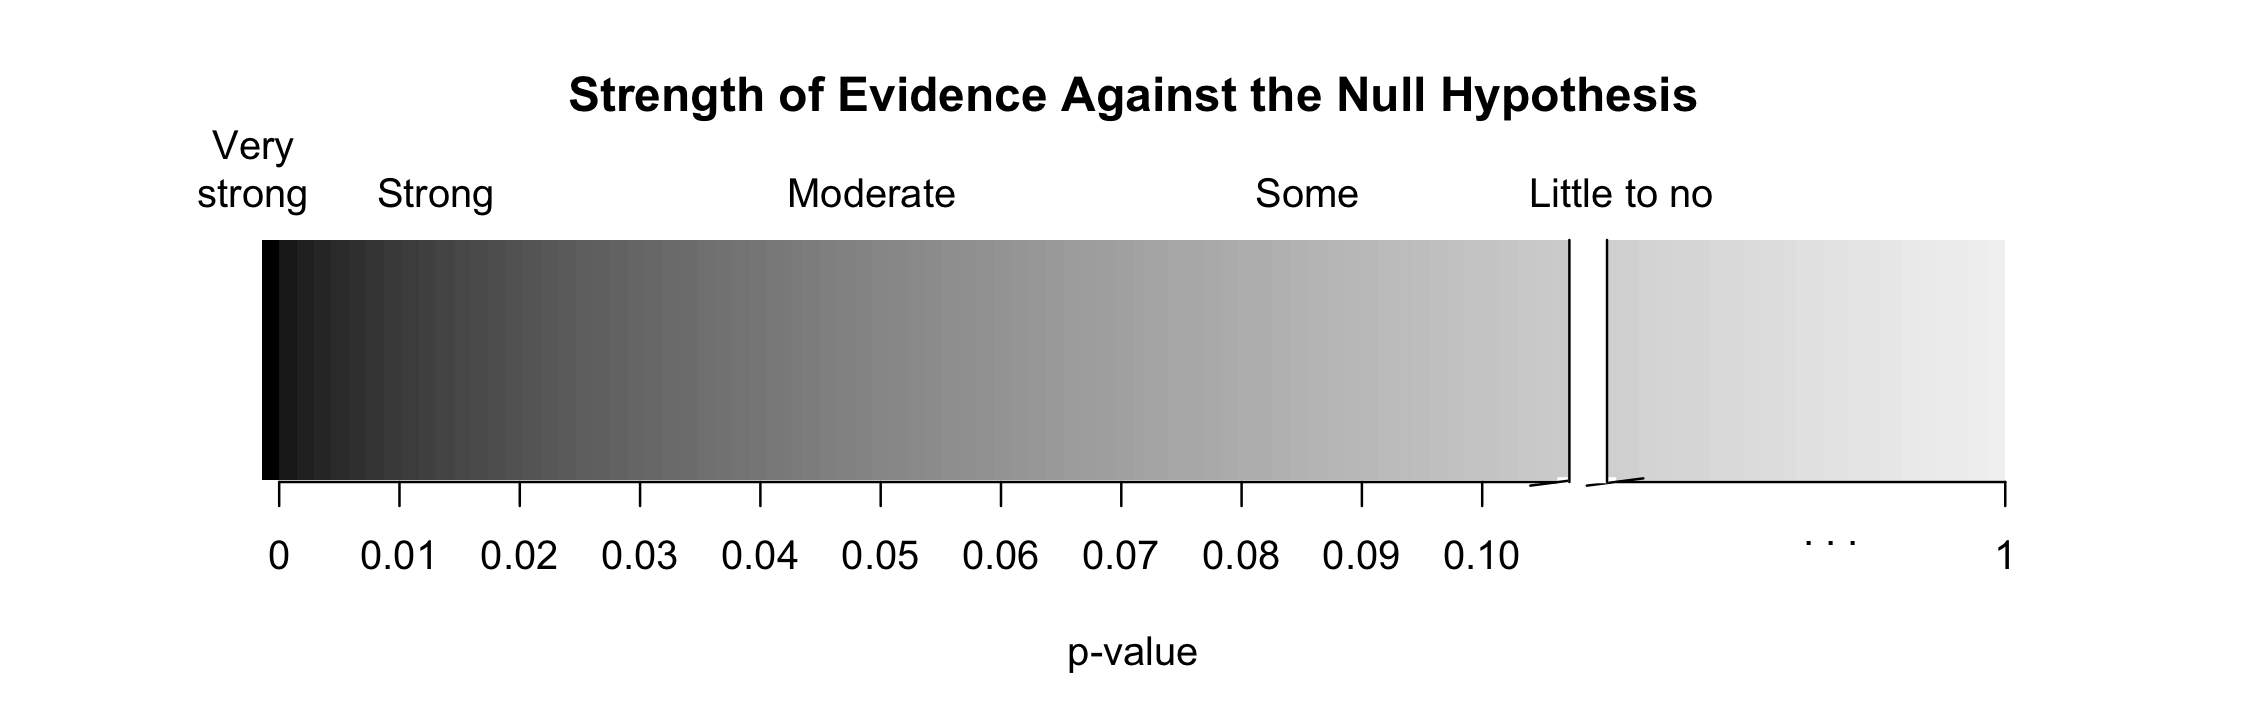
\includegraphics[width=0.9\linewidth]{images/soe_gradient_gray} \end{center}

\vspace{0.2in}

\begin{enumerate}
\def\labelenumi{\arabic{enumi}.}
\setcounter{enumi}{8}
\tightlist
\item
  Write a conclusion to the study in context of the problem.
\end{enumerate}

\vspace{0.8in}

\begin{enumerate}
\def\labelenumi{\arabic{enumi}.}
\setcounter{enumi}{9}
\tightlist
\item
  Would a 95\% confidence interval contain the null value of 0.2? Explain.
\end{enumerate}

\vspace{0.8in}

\begin{enumerate}
\def\labelenumi{\arabic{enumi}.}
\setcounter{enumi}{10}
\tightlist
\item
  What values should be entered for each of the following into the simulation to create the bootstrap distribution of sample proportions to find a 95\% confidence interval?
  \vspace{1mm}
\end{enumerate}

\begin{itemize}
\tightlist
\item
  Sample size:
\end{itemize}

\vspace{.1in}

\begin{itemize}
\tightlist
\item
  Number of successes:
\end{itemize}

\vspace{.1in}

\begin{itemize}
\tightlist
\item
  Number of repetitions:
\end{itemize}

\vspace{.1in}

\begin{itemize}
\tightlist
\item
  Confidence level (as a decimal):
\end{itemize}

\vspace{.1in}

\begin{Shaded}
\begin{Highlighting}[]
\FunctionTok{set.seed}\NormalTok{(}\DecValTok{216}\NormalTok{)}
\FunctionTok{one\_proportion\_bootstrap\_CI}\NormalTok{(}\AttributeTok{sample\_size =} \DecValTok{1753}\NormalTok{, }\CommentTok{\# Sample size}
                    \AttributeTok{number\_successes =} \DecValTok{328}\NormalTok{, }\CommentTok{\# Observed number of successes}
                    \AttributeTok{number\_repetitions =} \DecValTok{10000}\NormalTok{, }\CommentTok{\# Number of bootstrap samples to use}
                    \AttributeTok{confidence\_level =} \FloatTok{0.95}\NormalTok{) }\CommentTok{\# Confidence level as a decimal}
\end{Highlighting}
\end{Shaded}

\begin{center}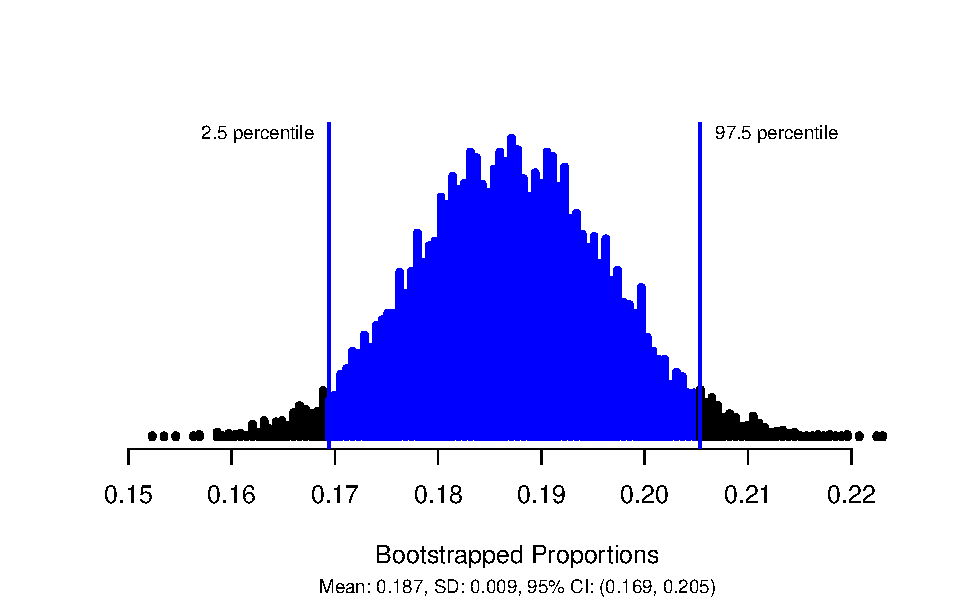
\includegraphics[width=0.7\linewidth]{05-UR-module3_review_files/figure-latex/unnamed-chunk-4-1} \end{center}

\begin{enumerate}
\def\labelenumi{\arabic{enumi}.}
\setcounter{enumi}{11}
\tightlist
\item
  Explain how to use cards to create one bootstrap sample.
\end{enumerate}

\vspace{1in}

\begin{enumerate}
\def\labelenumi{\arabic{enumi}.}
\setcounter{enumi}{12}
\tightlist
\item
  Report the 95\% confidence interval in interval notation.
\end{enumerate}

\vspace{0.2in}

\begin{enumerate}
\def\labelenumi{\arabic{enumi}.}
\setcounter{enumi}{13}
\tightlist
\item
  Interpret the 95\% confidence interval in context of the problem.
\end{enumerate}

\vspace{0.8in}

\newpage

\section{Module 4 Review - Theory-based Methods for a Single Proportion}\label{module-4-review---theory-based-methods-for-a-single-proportion}

Statistician Jessica Utts has conducted an extensive analysis of Ganzfeld studies that have investigated psychic functioning. Ganzfeld studies involve a ``sender'' and a ``receiver.'' Two people are placed in separate rooms. The sender looks at a ``target'' image on a television screen and attempts to transmit information about the target to the receiver. The receiver is then shown four possible choices or targets, one of which is the correct target and the other three are ``decoys.'' The receiver must choose the one he or she thinks best matches the description transmitted by the sender. If the correct target is chosen by the receiver, the session is a ``hit.'' Otherwise, it is a miss. Utts reported that her analysis considered a total of 2,124 sessions and found a total of 709 ``hits'' (Utts, 2010). Is there evidence of psychic ability?

\begin{enumerate}
\def\labelenumi{\arabic{enumi}.}
\tightlist
\item
  Write the parameter of interest in context of the study.
\end{enumerate}

\vspace{0.6in}

\begin{enumerate}
\def\labelenumi{\arabic{enumi}.}
\setcounter{enumi}{1}
\tightlist
\item
  Calculate the point estimate. Use proper notation.
\end{enumerate}

\vspace{0.3in}

\begin{enumerate}
\def\labelenumi{\arabic{enumi}.}
\setcounter{enumi}{2}
\tightlist
\item
  Write the null hypothesis in words.
\end{enumerate}

\vspace{0.6in}

\begin{enumerate}
\def\labelenumi{\arabic{enumi}.}
\setcounter{enumi}{3}
\tightlist
\item
  Write the alternative hypothesis in notation.
\end{enumerate}

\vspace{0.2in}

A single proportion can be mathematically modeled using the normal distribution if certain conditions are met.

Conditions for the sample distribution of \(\hat{p}\).

\begin{itemize}
\item
  Independence: The sample's observations are independent, e.g., are from a simple random sample
\item
  Large enough sample size:

  \begin{itemize}
  \tightlist
  \item
    Success-Failure Condition: There are at least 10 successes and 10 failures in the sample
  \end{itemize}
\end{itemize}

\[n \times \hat{p} \ge 10\] and \[n \times (1-\hat{p}) \ge 10\]

\newpage

\begin{enumerate}
\def\labelenumi{\arabic{enumi}.}
\setcounter{enumi}{4}
\tightlist
\item
  Are the conditions met to model the data with the Normal distribution?
\end{enumerate}

\vspace{0.6in}

Standardized sample proportion.

The standardized statistic for theory-based methods for one proportion is:

\[Z = \frac{\hat{p}-\pi_0}{SE_0(\hat{p})}\]

Where \[SE_0(\hat{p})=\sqrt\frac{\pi_0\times (1-\pi_0)}{n}\]

\begin{enumerate}
\def\labelenumi{\arabic{enumi}.}
\setcounter{enumi}{5}
\tightlist
\item
  Calculate the null standard error of the sample proportion
\end{enumerate}

\vspace{0.6in}

\begin{enumerate}
\def\labelenumi{\arabic{enumi}.}
\setcounter{enumi}{6}
\tightlist
\item
  Calculate the standardized statistic for the sample proportion.
\end{enumerate}

\vspace{0.4in}

\begin{figure}

{\centering 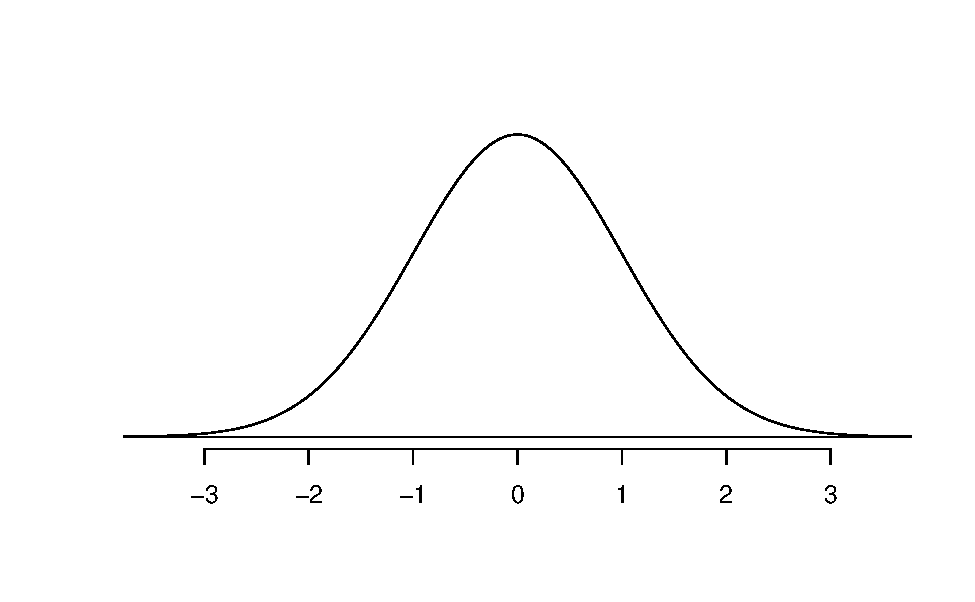
\includegraphics[width=0.5\linewidth]{05-UR-module4_review_files/figure-latex/simpleNormalcurve-1} 

}

\caption{A standard normal curve.}\label{fig:simpleNormalcurve}
\end{figure}

\begin{center}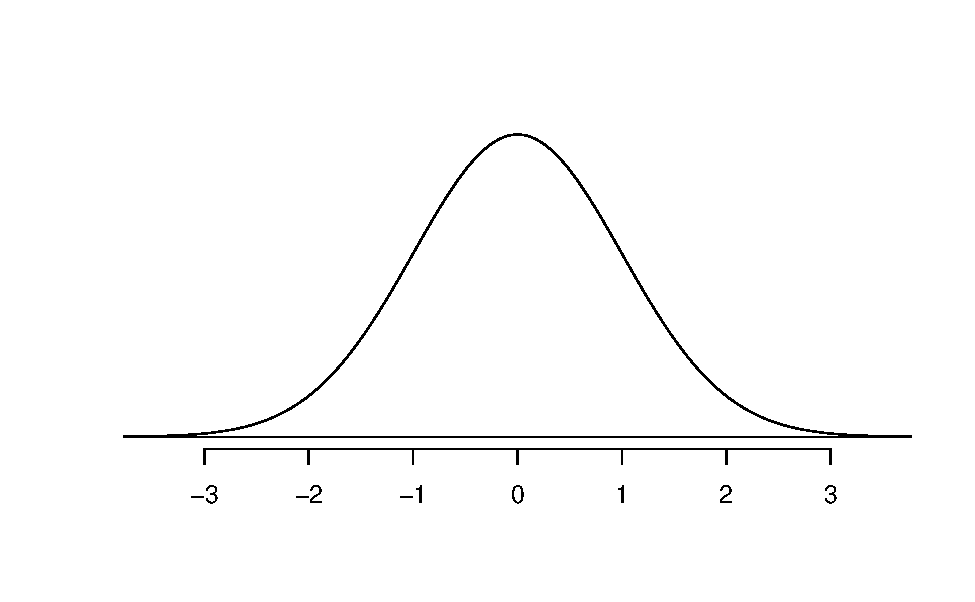
\includegraphics[width=0.5\linewidth]{05-UR-module4_review_files/figure-latex/Normcurve-1} \end{center}

\newpage

\begin{enumerate}
\def\labelenumi{\arabic{enumi}.}
\setcounter{enumi}{7}
\tightlist
\item
  Interpret the standardized statistic in context of the problem.
\end{enumerate}

\vspace{1in}

We will use the \texttt{pnorm()} function in \texttt{R} to find the p-value. The value of the standardized statistic calculated in question 8 is entered into the \texttt{R} code. We used \texttt{lower.tail\ =\ FALSE} to find the p-value so that \texttt{R} will calculate the p-value \emph{greater} than the value of the standardized statistic.

Notes:

\begin{itemize}
\tightlist
\item
  Use \texttt{lower.tail\ =\ TRUE} when doing a left-sided test.
\item
  Use \texttt{lower.tail\ =\ FALSE} when doing a right-sided test.
\item
  To find a two-sided p-value, use a left-sided test for negative Z or a right-sided test for positive Z, then multiply the value found by 2 to get the p-value.
\end{itemize}

\begin{Shaded}
\begin{Highlighting}[]
\FunctionTok{pnorm}\NormalTok{(}\FloatTok{9.333}\NormalTok{, }\CommentTok{\# Enter value of standardized statistic}
      \AttributeTok{m=}\DecValTok{0}\NormalTok{, }\AttributeTok{s=}\DecValTok{1}\NormalTok{, }\CommentTok{\# Using the standard normal mean = 0, sd = 1}
      \AttributeTok{lower.tail=}\ConstantTok{FALSE}\NormalTok{) }\CommentTok{\# Gives a p{-}value greater than the standardized statistic}
\CommentTok{\#\textgreater{} [1] 5.145792e{-}21}
\end{Highlighting}
\end{Shaded}

\begin{enumerate}
\def\labelenumi{\arabic{enumi}.}
\setcounter{enumi}{8}
\tightlist
\item
  Report the value of the p-value.
\end{enumerate}

\vspace{0.1in}

Simulation Method:

\begin{center}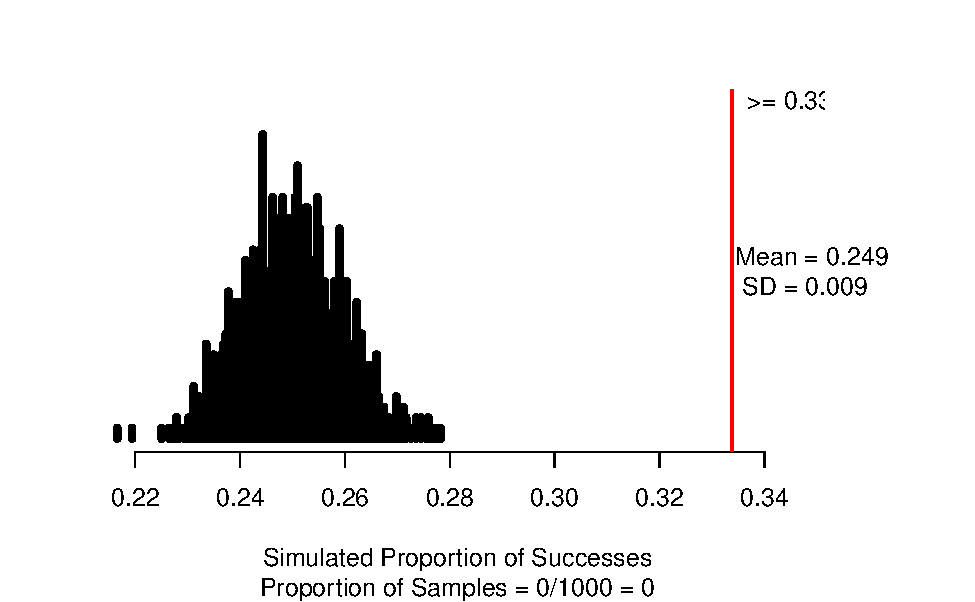
\includegraphics[width=0.85\linewidth]{05-UR-module4_review_files/figure-latex/unnamed-chunk-2-1} \end{center}

\begin{enumerate}
\def\labelenumi{\arabic{enumi}.}
\setcounter{enumi}{9}
\tightlist
\item
  Interpret the p-value in context of the study.
\end{enumerate}

\vspace{0.8in}

Next we will use theory-based methods to estimate the parameter of interest.

To calculate a theory-based 95\% confidence interval for \(\pi\), we will first find the \textbf{standard error} of \(\hat{p}\) by plugging in the value of \(\hat{p}\) for \(\pi\) in \(SD(\hat{p})\):

\[SE(\hat{p}) = \sqrt{\frac{\hat{p}\times(1-\hat{p})}{n}}.\]
Note that we do not include a ``0'' subscript, since we are not assuming a null hypothesis.

\begin{enumerate}
\def\labelenumi{\arabic{enumi}.}
\setcounter{enumi}{10}
\tightlist
\item
  Calculate the standard error of the sample proportion to find a 95\% confidence interval.
\end{enumerate}

\vspace{0.5in}

To find the confidence interval, we will add and subtract the \textbf{margin of error} to the point estimate:

\[\text{point estimate}\pm\text{margin of error}\]
\[\hat{p}\pm z^* SE(\hat{p})\]

The \(z^*\) multiplier is the percentile of a standard normal distribution that corresponds to our confidence level. If our confidence level is 95\%, we find the Z values that encompass the middle 95\% of the standard normal distribution. If 95\% of the standard normal distribution should be in the middle, that leaves 5\% in the tails, or 2.5\% in each tail. The \texttt{qnorm()} function in \texttt{R} will tell us the \(z^*\) value for the desired percentile (in this case, 95\% + 2.5\% = 97.5\% percentile).

\begin{figure}

{\centering 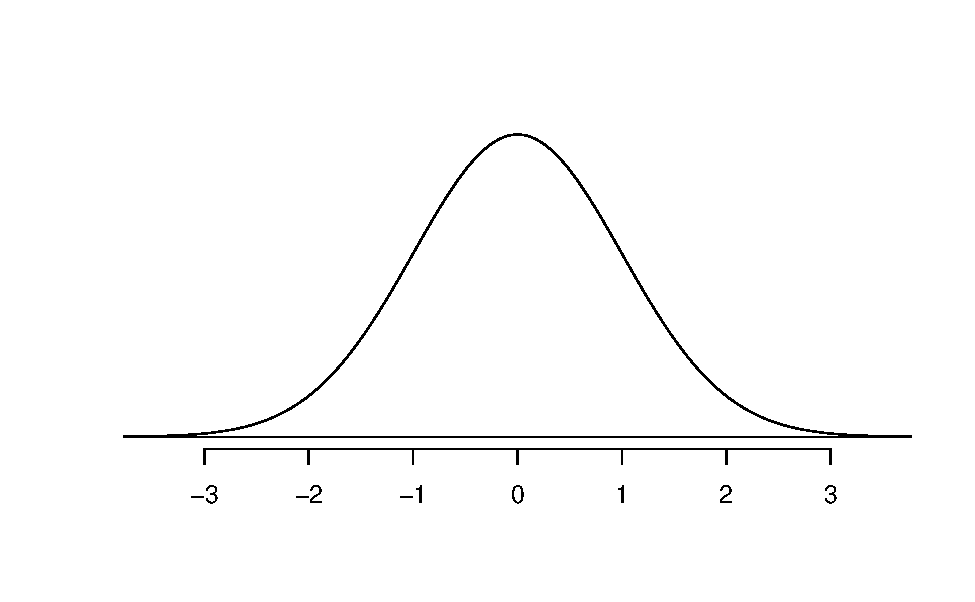
\includegraphics[width=0.5\linewidth]{05-UR-module4_review_files/figure-latex/Ncurve-1} 

}

\caption{A standard normal curve.}\label{fig:Ncurve}
\end{figure}

\begin{Shaded}
\begin{Highlighting}[]
\FunctionTok{qnorm}\NormalTok{(}\FloatTok{0.975}\NormalTok{) }\CommentTok{\# Multiplier for 95\% confidence interval}
\end{Highlighting}
\end{Shaded}

\begin{verbatim}
#> [1] 1.959964
\end{verbatim}

\begin{enumerate}
\def\labelenumi{\arabic{enumi}.}
\setcounter{enumi}{11}
\tightlist
\item
  Calculate the margin of error for a 95\% confidence interval for the true proportion of sessions that will result in a hit.
\end{enumerate}

\vspace{0.6in}

\begin{enumerate}
\def\labelenumi{\arabic{enumi}.}
\setcounter{enumi}{12}
\tightlist
\item
  Calculate the 95\% confidence interval for the true proportion of sessions that will result in a hit.
\end{enumerate}

\vspace{1in}

\newpage

Simulation Methods:

\begin{center}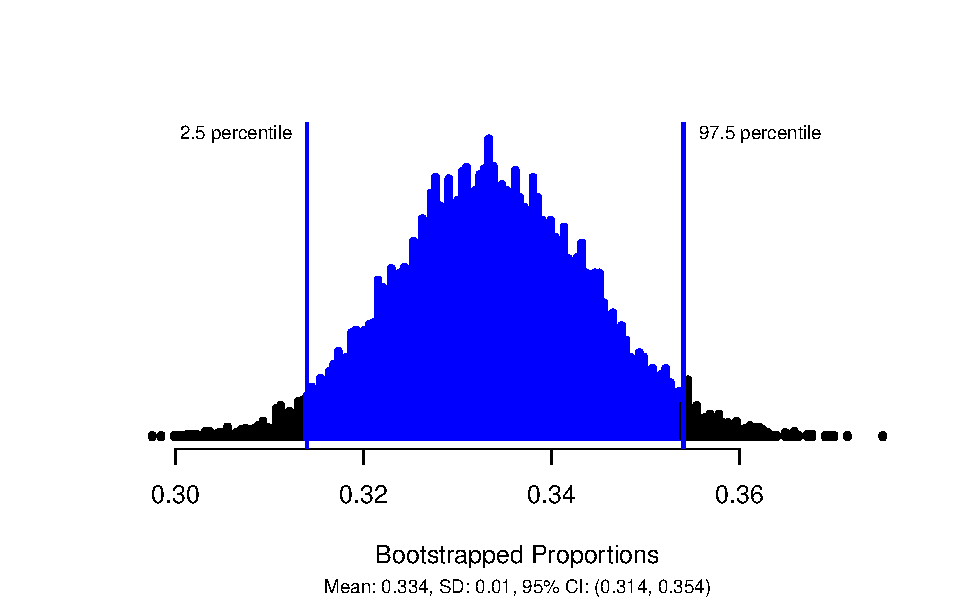
\includegraphics[width=0.85\linewidth]{05-UR-module4_review_files/figure-latex/unnamed-chunk-4-1} \end{center}

\begin{enumerate}
\def\labelenumi{\arabic{enumi}.}
\setcounter{enumi}{13}
\item
  Interpret the 95\% confidence interval in context of the problem.
  \vspace{0.6in}
\item
  Write a conclusion based on the p-value and the 95\% confidence interval.
\end{enumerate}

\vspace{0.6in}

\newpage

\chapter{Exploring Quantitative Data: Exploratory Data Analysis and Hypothesis Testing for a Single Quantitative Variable}\label{exploring-quantitative-data-exploratory-data-analysis-and-hypothesis-testing-for-a-single-quantitative-variable}

\section{Vocabulary Review and Key Topics}\label{vocabulary-review-and-key-topics-4}

Review the Golden Ticket posted in the resources at the end of the coursepack for a summary of a single quantitative variable.

\subsection{Key topics}\label{key-topics-5}

Module 6 will introduce exploratory data analysis and hypothesis testing using both simulation-based and theory-based methods for a single quantitative variable.
The \textbf{summary measure} for one quantitative variable is the \textbf{mean}.
Additionally, we can find the five number summary (min, Q1, median, Q3, max) as well as the sample standard deviation.

\begin{itemize}
\item
  Notation for a sample mean: \(\bar{x}\)
\item
  Notation for a sample standard deviation: \(s\)
\item
  Notation for a population mean: \(\mu\)
\item
  Notation for a population standard deviation: \(\sigma\)
\item
  Types of plots for a single categorical variable:

  \begin{itemize}
  \item
    Histogram
  \item
    Boxplot
  \item
    Dotplot
  \end{itemize}
\end{itemize}

\subsection{Vocabulary}\label{vocabulary-4}

\subsubsection*{Sample statistics for a single quantitative variable}\label{sample-statistics-for-a-single-quantitative-variable}
\addcontentsline{toc}{subsubsection}{Sample statistics for a single quantitative variable}

\begin{itemize}
\item
  \textbf{Mean}, \(\bar{x}\): the average
  \[ 
  \bar{x} = \frac{x_1 + x_2 + \cdots + x_n}{n},
  \]
  where \(x_1, x_2, \ldots, x_n\) are the data values and \(n\) is the sample size.
\item
  \textbf{Median}: value at the 50th percentile; approximately 50\% of data values are at or below the value of the median.
\end{itemize}

\vspace{1mm}

\begin{itemize}
\tightlist
\item
  \textbf{Quartile 1} (lower quartile), \(Q_1\): value at the 25th percentile; approximately 25\% of data values are at or below the value of \(Q_1\).
\end{itemize}

\vspace{1mm}

\begin{itemize}
\tightlist
\item
  \textbf{Quartile 3} (upper quartile), \(Q_3\): value at the 75th percentile; approximately 75\% of data values are at or below the value of \(Q_3\).
\end{itemize}

\newpage

\begin{itemize}
\item
  \textbf{Sample standard deviation}, \(s\): on average, each value in the data set is \(s\) units from the mean of the data set (\(\bar{x}\)). We will always calculate \(s\) using R, but it is calculated using the following formula:
  \[
  s = \sqrt{\frac{(x_1-\bar{x})^2 + (x_2-\bar{x})^2 + \cdots + (x_n-\bar{x})^2}{n}},
  \]
  where \(x_1, x_2, \ldots, x_n\) are the data values, \(\bar{x}\) is the sample mean, and \(n\) is the sample size.
\item
  \textbf{Interquartile range}: the range of the data between the two quartiles: \(IQR = Q_3-Q_1\).
\item
  R code to find the summary statistics for a quantitative variable:

\begin{Shaded}
\begin{Highlighting}[]
\NormalTok{object }\SpecialCharTok{\%\textgreater{}\%} \CommentTok{\# Data set piped into...}
    \FunctionTok{summarise}\NormalTok{(}\FunctionTok{favstats}\NormalTok{(variable))}
\end{Highlighting}
\end{Shaded}
\end{itemize}

\subsubsection*{Plotting one quantitative variable}\label{plotting-one-quantitative-variable}
\addcontentsline{toc}{subsubsection}{Plotting one quantitative variable}

\begin{itemize}
\item
  \textbf{Histogram}: sorts a quantitative variable into bins of a certain width. R code to create a histogram:

\begin{Shaded}
\begin{Highlighting}[]
\NormalTok{object }\SpecialCharTok{\%\textgreater{}\%} \CommentTok{\# Data set piped into...}
    \FunctionTok{ggplot}\NormalTok{(}\FunctionTok{aes}\NormalTok{(}\AttributeTok{x =}\NormalTok{ variable)) }\SpecialCharTok{+}   \CommentTok{\# Name variable to plot}
    \FunctionTok{geom\_histogram}\NormalTok{(}\AttributeTok{binwidth =} \DecValTok{10}\NormalTok{) }\SpecialCharTok{+}  \CommentTok{\# Create histogram with specified binwidth}
    \FunctionTok{labs}\NormalTok{(}\AttributeTok{title =} \StringTok{"Don\textquotesingle{}t forget to title the plot!"}\NormalTok{, }\CommentTok{\# Title for plot}
        \AttributeTok{x =} \StringTok{"x{-}axis label"}\NormalTok{, }\CommentTok{\# Label for x axis}
        \AttributeTok{y =} \StringTok{"y{-}axis label"}\NormalTok{) }\CommentTok{\# Label for y axis}
\end{Highlighting}
\end{Shaded}
\item
  \textbf{Boxplot}: plots the values of the five-number summary and shows any outliers in the data set. R code to create a boxplot:

\begin{Shaded}
\begin{Highlighting}[]
\NormalTok{object }\SpecialCharTok{\%\textgreater{}\%} \CommentTok{\# Data set piped into...}
    \FunctionTok{ggplot}\NormalTok{(}\FunctionTok{aes}\NormalTok{(}\AttributeTok{x =}\NormalTok{ variable)) }\SpecialCharTok{+} \CommentTok{\# Name variable to plot}
    \FunctionTok{geom\_boxplot}\NormalTok{() }\SpecialCharTok{+} \CommentTok{\# Create boxplot }
    \FunctionTok{labs}\NormalTok{(}\AttributeTok{title =} \StringTok{"Don\textquotesingle{}t forget to title the plot!"}\NormalTok{, }\CommentTok{\# Title for plot}
        \AttributeTok{x =} \StringTok{"x{-}axis label"}\NormalTok{, }\CommentTok{\# Label for x axis}
        \AttributeTok{y =} \StringTok{"y{-}axis label"}\NormalTok{) }\CommentTok{\# Label for y axis}
\end{Highlighting}
\end{Shaded}
\item
  \textbf{Dotplot}: plots each value as a dot along the \(x\)-axis. R code to create a dotplot:

\begin{Shaded}
\begin{Highlighting}[]
\NormalTok{object }\SpecialCharTok{\%\textgreater{}\%} \CommentTok{\# Data set piped into...}
    \FunctionTok{ggplot}\NormalTok{(}\FunctionTok{aes}\NormalTok{(}\AttributeTok{x =}\NormalTok{ variable)) }\SpecialCharTok{+} \CommentTok{\# Name variable to plot}
    \FunctionTok{geom\_dotplot}\NormalTok{() }\SpecialCharTok{+} \CommentTok{\# Create dotplot }
    \FunctionTok{labs}\NormalTok{(}\AttributeTok{title =} \StringTok{"Don\textquotesingle{}t forget to title the plot!"}\NormalTok{, }\CommentTok{\# Title for plot}
        \AttributeTok{x =} \StringTok{"x{-}axis label"}\NormalTok{, }\CommentTok{\# Label for x axis}
        \AttributeTok{y =} \StringTok{"y{-}axis label"}\NormalTok{) }\CommentTok{\# Label for y axis}
\end{Highlighting}
\end{Shaded}
\item
  Four characteristics of a distribution of a single quantitative variable:

  \begin{itemize}
  \item
    Shape (symmetric, skewed left, or skewed right)
  \item
    Center
  \item
    Spread
  \item
    Outliers?
  \end{itemize}
\end{itemize}

\newpage

\subsubsection*{Hypothesis testing for a single mean}\label{hypothesis-testing-for-a-single-mean}
\addcontentsline{toc}{subsubsection}{Hypothesis testing for a single mean}

\begin{itemize}
\tightlist
\item
  \textbf{Hypotheses in notation for a single mean}: In the hypotheses below, \(\mu_0\) is the \textbf{null value}.
\end{itemize}

\[H_0: \mu = \mu_0\]
\[H_A: \mu\left\{
\begin{array}{ll}
< \\
\ne \\
< \\
\end{array}
\right\}
\mu_0 \]

\subsubsection*{Simulation-based hypothesis testing}\label{simulation-based-hypothesis-testing}
\addcontentsline{toc}{subsubsection}{Simulation-based hypothesis testing}

\begin{itemize}
\item
  \textbf{Conditions necessary to use simulation-based methods for inference for a single quantitative variable}:

  \begin{itemize}
  \tightlist
  \item
    \textbf{Independence}: observational units must be independent of one another.
  \end{itemize}
\item
  \textbf{Simulation-based methods to create the null distribution}: R code to use for simulation-based methods for one quantitative variable to find the p-value, \texttt{one\_mean\_test} (from the \texttt{catstats} package), is shown below. Review the comments (instructions after the \#) to see what each should be entered for each line of code.

\begin{Shaded}
\begin{Highlighting}[]
\FunctionTok{one\_mean\_test}\NormalTok{(object}\SpecialCharTok{$}\NormalTok{variable,}\CommentTok{\#Enter the object name and variable}
          \AttributeTok{null\_value =}\NormalTok{ xx, }\CommentTok{\#Enter the null value for the study}
          \AttributeTok{summary\_measure =} \StringTok{"mean"}\NormalTok{,  }\CommentTok{\#Can choose between mean or median}
          \AttributeTok{shift =}\NormalTok{ xx, }\CommentTok{\#Difference between the null value and the sample mean}
          \AttributeTok{as\_extreme\_as =}\NormalTok{ xx, }\CommentTok{\#Value of the summary statistic}
          \AttributeTok{direction =} \StringTok{"xx"}\NormalTok{, }\CommentTok{\#Specify direction of alternative hypothesis}
          \AttributeTok{number\_repetitions =} \DecValTok{10000}\NormalTok{)}
\end{Highlighting}
\end{Shaded}
\end{itemize}

\subsubsection*{Theory-based hypothesis testing}\label{theory-based-hypothesis-testing}
\addcontentsline{toc}{subsubsection}{Theory-based hypothesis testing}

\begin{itemize}
\item
  Theory-based methods should give the same results as simulation-based methods if conditions are met. For a single quantitative variable, conditions are met if either the data themselves follow a normal distribution or if the sample size is large enough. We call this the ``normality condition.''
\item
  \textbf{Conditions for the sampling distribution of \(\bar{x}\) to follow an approximate normal distribution}:

  \begin{itemize}
  \item
    \textbf{Independence}: the sample's observations are independent, e.g., are from a simple random sample. (\emph{Remember}: This also must be true to use simulation methods!)
  \item
    \textbf{Normality Condition}: either the sample observations come from a normally distributed population or we have a large enough sample size. To check this condition, use the following rules of thumb:

    \begin{itemize}
    \item
      \(n < 30\): The distribution of the sample must be approximately normal with no outliers.
    \item
      \(30 \le n < 100\): We can relax the condition a little; the distribution of the sample must have no extreme outliers or skewness.
    \item
      \(n \ge 100\): Can assume the sampling distribution of \(\bar{x}\) is nearly normal, even if the underlying distribution of individual observations is not.
    \end{itemize}
  \end{itemize}
\item
  \textbf{t-distribution}: a theoretical distribution that is bell-shaped with mean zero. Its degrees of freedom determine the variability of the distribution. For very large degrees of freedom, the \(t\)-distribution is close to a standard normal distribution. For a single quantitative variable, the degrees of freedom are calculated by subtracting one from the sample size: \(n-1\). A \(t\)-distribution with \(n-1\) degrees of freedom is denoted by: \(t_{n-1}\).
\item
  \textbf{Standard error of the sample mean}: measures the how far each possible sample mean is from the true mean, on average, and is calculated using the formula below:
  \[SE(\bar{x})=\frac{s}{\sqrt{n}}\]
  where \(s\) is the sample standard deviation.

  \begin{itemize}
  \tightlist
  \item
    For inference involving means, the formula for the standard error will be the same for both hypothesis tests and confidence intervals (unlike inference involving proportions, where the standard error for a hypothesis test used the null value in the calculation).
  \end{itemize}
\item
  \textbf{Standardized sample mean}: standardized statistic for a single quantitative variable calculated using:
  \[
  T = \frac{\bar{x} - \mu_0}{SE(\bar{x})},
  \]
  If the conditions for the sampling distribution of \(\bar{x}\) to follow an approximate normal distribution are met, and if the true value of \(\mu\) is equal to the null value of \(\mu_0\), the standardized sample mean, \(T\), will have an approximate \(t\)-distribution with \(n-1\) degrees of freedom.
\item
  The theory-based \textbf{p-value} for hypothesis testing involving means can be found in R by using the \texttt{pt} function to find the probability of the observed standardized statistic or one more extreme (in the direction of \(H_A\)). This probability is the area under a \emph{\(t\)-distribution with the appropriate degrees of freedom} at or more extreme than the observed standardized statistic.

  \begin{itemize}
  \item
    \texttt{pt} will give you a p-value using the \(t\)-distribution with a given degrees of freedom (enter for \texttt{yy}). For a single mean, \texttt{df} = \(n - 1\).
  \item
    Enter the value of the standardized statistic for \texttt{xx}
  \item
    If a ``greater than'' alternative, change \texttt{lower.tail\ =\ TRUE} to \texttt{FALSE}.
  \item
    If a two-sided test, multiply by 2.
  \end{itemize}

\begin{Shaded}
\begin{Highlighting}[]
\FunctionTok{pt}\NormalTok{(xx, }\AttributeTok{df =}\NormalTok{ yy, }\AttributeTok{lower.tail=}\ConstantTok{TRUE}\NormalTok{)}
\end{Highlighting}
\end{Shaded}
\end{itemize}

\newpage

\section{Video Notes: Exploratory Data Analysis and Hypothesis Testing of Quantitative Variables}\label{video-notes-exploratory-data-analysis-and-hypothesis-testing-of-quantitative-variables}

Read Chapters 5 and 17 in the course textbook. Use the following videos to complete the video notes for Module 6.

\subsection{Course Videos}\label{course-videos-4}

\begin{itemize}
\item
  QuantitativeData
\item
  5.5to5.6
\item
  5.7
\item
  17.2
\item
  17.3TheoryTests
\end{itemize}

\setstretch{1}

\subsection*{Summarizing quantitative data - Videos 5.2to5.4 and 5.5to5.6}\label{summarizing-quantitative-data---videos-5.2to5.4-and-5.5to5.6}
\addcontentsline{toc}{subsection}{Summarizing quantitative data - Videos 5.2to5.4 and 5.5to5.6}

\subsubsection*{Types of plots}\label{types-of-plots}
\addcontentsline{toc}{subsubsection}{Types of plots}

We will revisit the moving to Montana data set and plot the age of the buyers.

Dotplot:

\vspace{0.5in}

\begin{Shaded}
\begin{Highlighting}[]
\NormalTok{moving }\SpecialCharTok{\%\textgreater{}\%}
  \FunctionTok{ggplot}\NormalTok{(}\FunctionTok{aes}\NormalTok{(}\AttributeTok{x =}\NormalTok{ Age))}\SpecialCharTok{+} \CommentTok{\#Enter variable to plot}
  \FunctionTok{geom\_dotplot}\NormalTok{() }\SpecialCharTok{+} 
  \FunctionTok{labs}\NormalTok{(}\AttributeTok{title =} \StringTok{"Dotplot of Age of Buyers from Gallatin }
\StringTok{       County Home Sales"}\NormalTok{, }\CommentTok{\#Title your plot}
       \AttributeTok{x =} \StringTok{"Age"}\NormalTok{, }\CommentTok{\#x{-}axis label}
       \AttributeTok{y =} \StringTok{"Proportion"}\NormalTok{) }\CommentTok{\#y{-}axis label}
\end{Highlighting}
\end{Shaded}

\begin{center}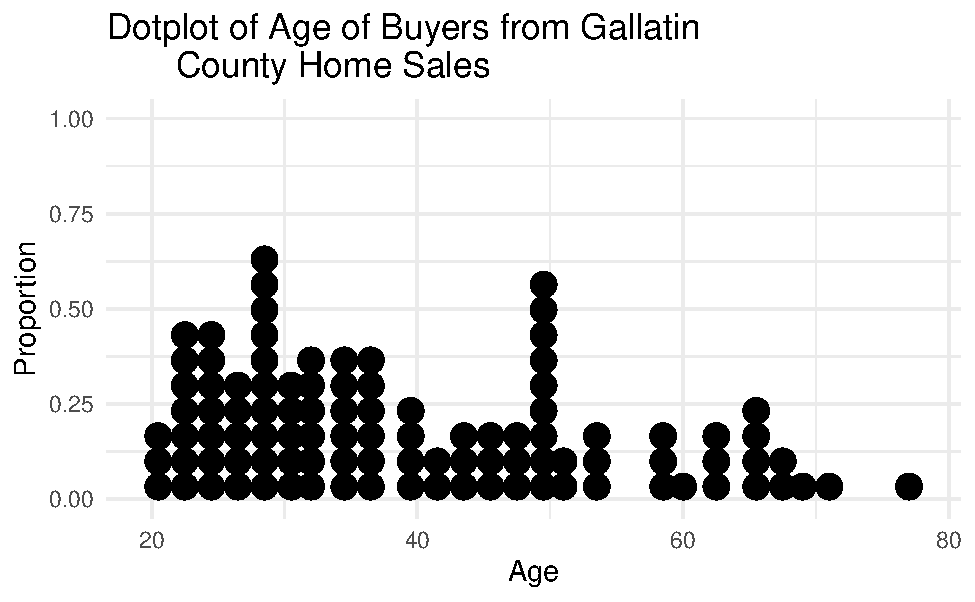
\includegraphics[width=0.75\linewidth]{06-VN06-EDAonemeanSim_files/figure-latex/unnamed-chunk-2-1} \end{center}

\newpage

Histogram:

\vspace{0.2in}

\begin{Shaded}
\begin{Highlighting}[]
\NormalTok{moving }\SpecialCharTok{\%\textgreater{}\%}
  \FunctionTok{ggplot}\NormalTok{(}\FunctionTok{aes}\NormalTok{(}\AttributeTok{x =}\NormalTok{ Age))}\SpecialCharTok{+}
  \FunctionTok{geom\_histogram}\NormalTok{(}\AttributeTok{binwidth =} \DecValTok{7}\NormalTok{) }\SpecialCharTok{+} 
  \FunctionTok{labs}\NormalTok{(}\AttributeTok{title =} \StringTok{"Histogram of Age of Buyers from Gallatin }
\StringTok{       County Home Sales"}\NormalTok{,}
       \CommentTok{\#Title your plot}
       \AttributeTok{x =} \StringTok{"Age"}\NormalTok{,}
       \AttributeTok{y =} \StringTok{"Count"}\NormalTok{)}
\end{Highlighting}
\end{Shaded}

\begin{center}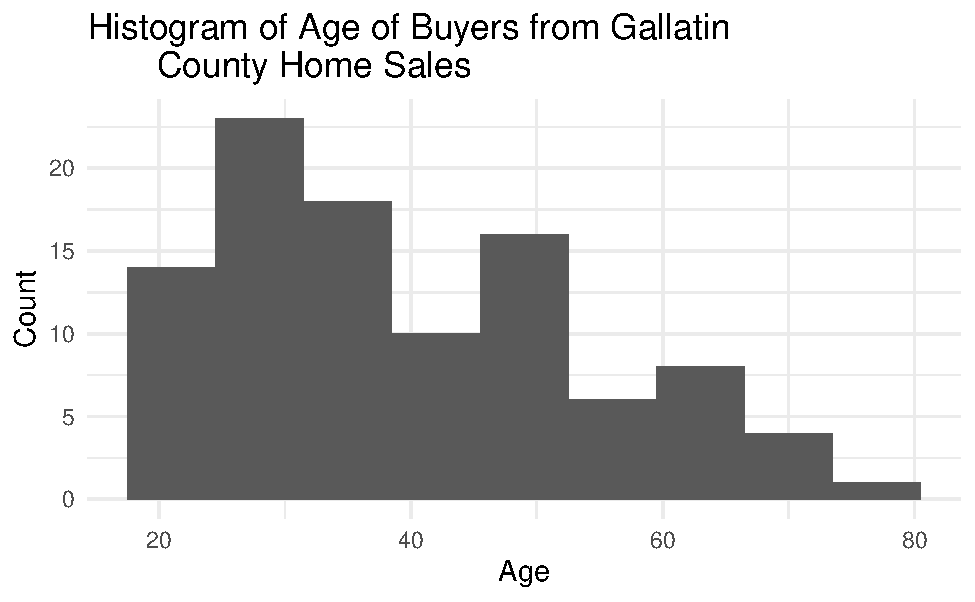
\includegraphics[width=0.7\linewidth]{06-VN06-EDAonemeanSim_files/figure-latex/unnamed-chunk-3-1} \end{center}

\setstretch{1.5}

Quantitative data can be numerically summarized by finding:

Two measures of center:

\begin{itemize}
\item
  Mean: \_\_\_\_\_\_\_\_\_\_\_\_ of all the \_\_\_\_\_\_\_\_\_\_\_\_\_ in the data set.

  \begin{itemize}
  \tightlist
  \item
    Sum the values in the data set and divide
    the sum by the sample size
  \end{itemize}
\item
  Notation used for the population mean:

  \begin{itemize}
  \tightlist
  \item
    Single quantitative variable:
  \end{itemize}
\end{itemize}

\vspace{0.1in}

\rgi \rgi - One categorical and one quantitative variable:

\vspace{0.1in}

\rgi \rgi \rgi - Subscripts represent the \_\_\_\_\_\_\_\_\_\_\_ variable groups

\begin{itemize}
\tightlist
\item
  Notation used for the sample mean:
\end{itemize}

\rgi \rgi - Single quantitative variable:

\vspace{0.1in}

\rgi \rgi - One categorical and one quantitative variable:

\vspace{0.1in}

\begin{itemize}
\item
  Median: Value at the \_\_\_\_\_\_\_\_\_\_\_\_\_ percentile

  \begin{itemize}
  \item
    \_\_\_\_\_\_\_\_\_\_ \% of values are at and \_\_\_\_\_\_\_\_\_\_\_ and at and \_\_\_\_\_\_\_\_\_\_\_ the value of the \_\_\_\_\_\_\_\_\_\_\_\_\_\_.
  \item
    Middle value in a list of ordered values
  \end{itemize}
\end{itemize}

Two measures of spread:

\begin{itemize}
\tightlist
\item
  Standard deviation: Average \_\_\_\_\_\_\_\_\_\_\_\_\_\_\_\_\_\_\_ each data point is from the \_\_\_\_\_\_\_\_\_\_\_\_\_\_ of the data set.
\end{itemize}

\vspace{1mm}

\rgi \rgi - Notation used for the population standard deviation

\vspace{0.2in}

\rgi \rgi - Notation used for the sample standard deviation

\vspace{0.2in}

\begin{itemize}
\tightlist
\item
  Interquartile range: middle 50\% of data values
\end{itemize}

\rgi Formula:

\rgi \rgi Quartile 3 (Q3) - value at the 75th percentile

\rgi \rgi - \_\_\_\_\_\_\_\_\_\_\_\_ \% of values are at and \_\_\_\_\_\_\_\_\_\_\_\_\_ the value of Q3

\rgi \rgi Quartile 1 (Q1) - value at the 25th percentile

\rgi \rgi - \_\_\_\_\_\_\_\_\_\_\_\_\_ \% of values are at and \_\_\_\_\_\_\_\_\_\_\_\_\_ the value of Q1

\vspace{1mm}

\setstretch{1}

\newpage

Boxplot (3rd type of plot for quantitative variables)

\begin{verbatim}
- Five number summary: minimum, Q1, median, Q3, maximum
\end{verbatim}

\vspace{0.3in}

\begin{Shaded}
\begin{Highlighting}[]
\NormalTok{moving }\SpecialCharTok{\%\textgreater{}\%}
  \FunctionTok{ggplot}\NormalTok{(}\FunctionTok{aes}\NormalTok{(}\AttributeTok{x =}\NormalTok{ Age))}\SpecialCharTok{+} \CommentTok{\#Enter variable to plot}
  \FunctionTok{geom\_boxplot}\NormalTok{() }\SpecialCharTok{+} 
  \FunctionTok{labs}\NormalTok{(}\AttributeTok{title =} \StringTok{"Boxplot of Age of Buyers from Gallatin }
\StringTok{       County Home Sales"}\NormalTok{, }\CommentTok{\#Title your plot}
       \AttributeTok{x =} \StringTok{"Age"}\NormalTok{, }\CommentTok{\#x{-}axis label}
       \AttributeTok{y =} \StringTok{""}\NormalTok{) }\CommentTok{\#y{-}axis label}
\end{Highlighting}
\end{Shaded}

\begin{center}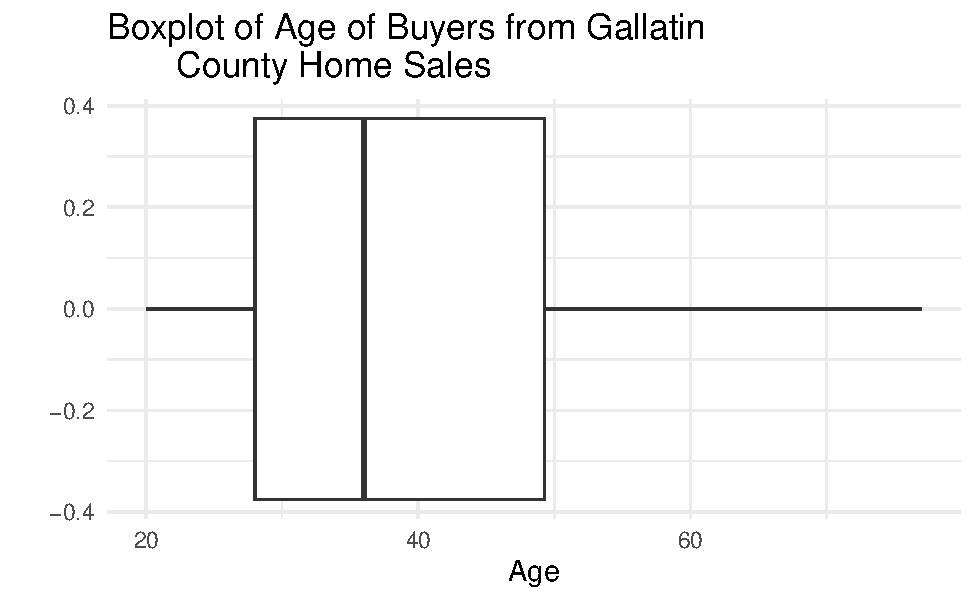
\includegraphics[width=0.7\linewidth]{06-VN06-EDAonemeanSim_files/figure-latex/unnamed-chunk-4-1} \end{center}

\begin{Shaded}
\begin{Highlighting}[]
\FunctionTok{favstats}\NormalTok{(moving}\SpecialCharTok{$}\NormalTok{Age)}
\end{Highlighting}
\end{Shaded}

\begin{verbatim}
#>  min Q1 median    Q3 max  mean       sd   n missing
#>   20 28     36 49.25  77 39.77 14.35471 100       0
\end{verbatim}

Interpret the value of \(Q_3\) for the age of buyers.

\vspace{0.5in}

Interpret the value of s for the age of buyers.

\vspace{0.5in}

\newpage

\subsubsection*{Four characteristics of plots for quantitative variables}\label{four-characteristics-of-plots-for-quantitative-variables}
\addcontentsline{toc}{subsubsection}{Four characteristics of plots for quantitative variables}

\begin{itemize}
\tightlist
\item
  Shape: overall pattern of the data
\end{itemize}

\begin{center}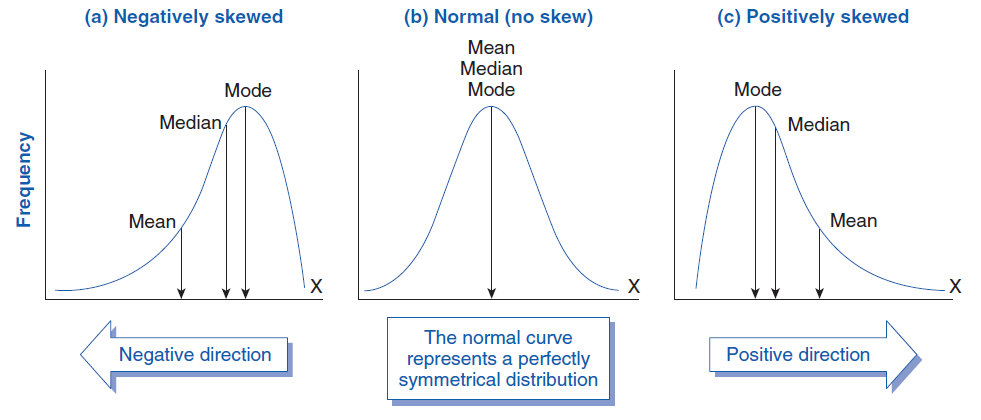
\includegraphics[width=0.8\linewidth]{images/shape2} \end{center}

\rgi \rgi - What is the shape of the distribution of age of buyers for Gallatin County home sales?

\vspace{0.3in}

\begin{itemize}
\tightlist
\item
  Center:
\end{itemize}

\rgi Mean or Median

\rgi \rgi - Report the measure of center for the boxplot of age of buyers for Gallatin County home sales.

\vspace{0.3in}

\begin{itemize}
\tightlist
\item
  Spread (or variability):
\end{itemize}

\rgi Standard deviation or IQR

\rgi \rgi - Report the IQR for the distribution of age of buyers from Gallatin County home sales.

\vspace{0.3in}

\begin{itemize}
\tightlist
\item
  Outliers?
\end{itemize}

\rgi values \textless{} \(Q_1 - 1.5 \times IQR\)

\rgi values \textgreater{} \(Q_3 + 1.5 \times IQR\)

\rgi \rgi - Use these formulas to show that there are no outliers in the distribution of age of buyers from Gallatin County home sales.

\vspace{0.8in}
\newpage

Let's look at side-by-side boxplot of the variable age by state of origin moved from.

\begin{Shaded}
\begin{Highlighting}[]
\NormalTok{moving }\SpecialCharTok{\%\textgreater{}\%}  \CommentTok{\# Data set piped into...}
  \FunctionTok{ggplot}\NormalTok{(}\FunctionTok{aes}\NormalTok{(}\AttributeTok{y =}\NormalTok{ Age, }\AttributeTok{x =}\NormalTok{ From))}\SpecialCharTok{+}  \CommentTok{\# Identify variables}
  \FunctionTok{geom\_boxplot}\NormalTok{()}\SpecialCharTok{+}  \CommentTok{\# Tell it to make a box plot}
  \FunctionTok{labs}\NormalTok{(}\AttributeTok{title =} \StringTok{"Side by side box plot of Age by State of Origin }
\StringTok{  of Buyers from Gallatin County Home Sales"}\NormalTok{,  }\CommentTok{\# Title}
       \AttributeTok{x =} \StringTok{"State of Origin"}\NormalTok{,    }\CommentTok{\# x{-}axis label}
       \AttributeTok{y =} \StringTok{"Age"}\NormalTok{)  }\CommentTok{\# y{-}axis label}
\end{Highlighting}
\end{Shaded}

\begin{center}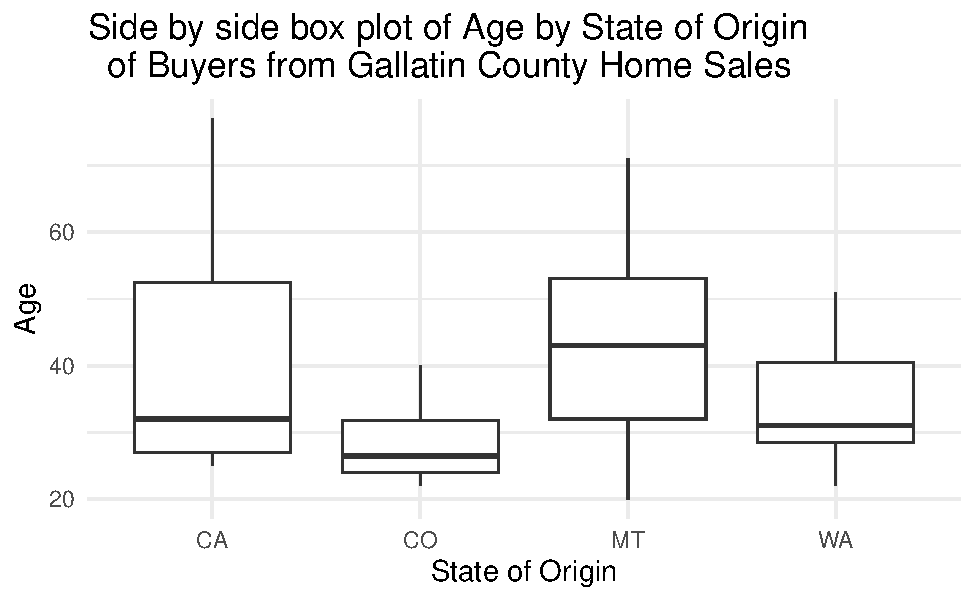
\includegraphics[width=0.85\linewidth]{06-VN06-EDAonemeanSim_files/figure-latex/unnamed-chunk-7-1} \end{center}

\begin{itemize}
\tightlist
\item
  Which state of origin had the oldest median age of buyers from sampled home sales?
\end{itemize}

\vspace{0.4in}

\begin{itemize}
\tightlist
\item
  Which state of origin had the most variability in age of buyers from sampled home sales?
\end{itemize}

\vspace{0.4in}

\begin{itemize}
\tightlist
\item
  Which state of origin had the most symmetric distribution of ages of buyers from sampled home sales?
\end{itemize}

\vspace{0.4in}

\begin{itemize}
\tightlist
\item
  Which state of origin had outliers for the age of buyers from sampled home sales?
\end{itemize}

\vspace{0.4in}

\newpage

\subsubsection*{Robust statistics - Video 5.7}\label{robust-statistics---video-5.7}
\addcontentsline{toc}{subsubsection}{Robust statistics - Video 5.7}

Let's review the summary statistics and histogram of age of buyers from sampled home sales.

\begin{center}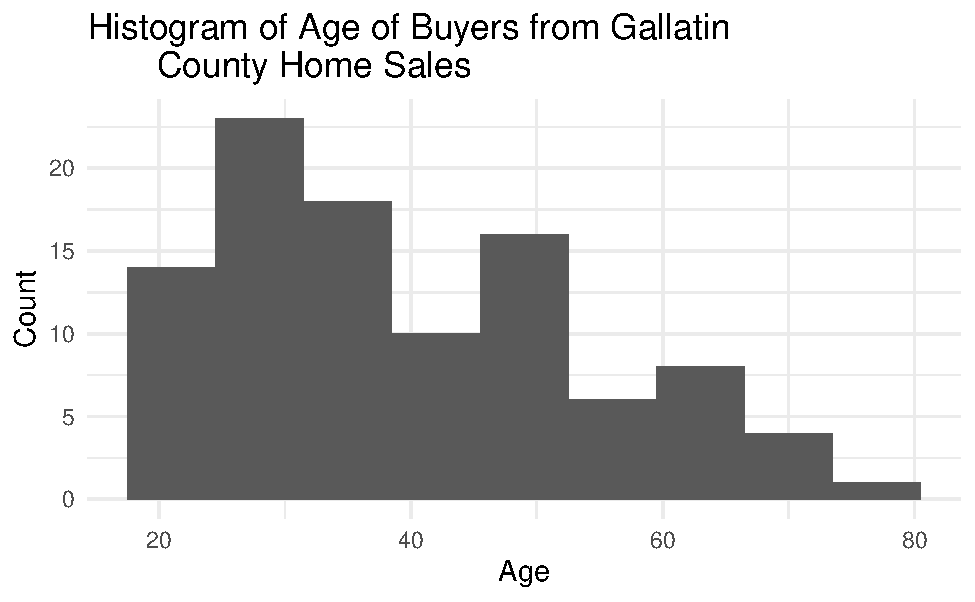
\includegraphics[width=0.85\linewidth]{06-VN06-EDAonemeanSim_files/figure-latex/unnamed-chunk-8-1} \end{center}

\begin{verbatim}
#>  min Q1 median    Q3 max  mean       sd   n missing
#>   20 28     36 49.25  77 39.77 14.35471 100       0
\end{verbatim}

\setstretch{1.5}

Notice that the \_\_\_\_\_\_\_\_\_\_\_\_\_ has been pulled in the direction of the \_\_\_\_\_\_\_\_\_\_\_\_\_\_\_.

\begin{itemize}
\item
  The \_\_\_\_\_\_\_\_\_\_\_ is a robust measure of center.
\item
  The \_\_\_\_\_\_\_\_\_\_\_ is a robust measure of spread.
\item
  Robust means not \_\_\_\_\_\_\_\_\_\_\_\_\_\_\_\_\_ by outliers.
\end{itemize}

When the distribution is symmetric use the \_\_\_\_\_\_\_\_\_\_\_\_ as the measure of center and the \_\_\_\_\_\_\_\_\_\_\_ as the measure of spread.

When the distribution is skewed with outliers use the \_\_\_\_\_\_\_\_\_\_\_\_\_ as the measure of center and the \_\_\_\_\_\_\_\_\_\_\_\_ as the measure of spread.

\setstretch{1}

\newpage

\subsection{Video notes single quantitative variable inference}\label{video-notes-single-quantitative-variable-inference}

\setstretch{1}

Example: What is the average weight of adult male polar bears? The weight was measured on a representative sample of 83 male polar bears from the Southern Beaufort Sea.

\begin{Shaded}
\begin{Highlighting}[]
\NormalTok{pb }\OtherTok{\textless{}{-}} \FunctionTok{read.csv}\NormalTok{(}\StringTok{"https://math.montana.edu/courses/s216/data/polarbear.csv"}\NormalTok{)}
\end{Highlighting}
\end{Shaded}

Plots of the data:

\begin{Shaded}
\begin{Highlighting}[]
\NormalTok{pb }\SpecialCharTok{\%\textgreater{}\%}
    \FunctionTok{ggplot}\NormalTok{(}\FunctionTok{aes}\NormalTok{(}\AttributeTok{x =}\NormalTok{ Weight)) }\SpecialCharTok{+}   \CommentTok{\# Name variable to plot}
    \FunctionTok{geom\_histogram}\NormalTok{(}\AttributeTok{binwidth =} \DecValTok{10}\NormalTok{) }\SpecialCharTok{+}  \CommentTok{\# Create histogram with specified binwidth}
    \FunctionTok{labs}\NormalTok{(}\AttributeTok{title =} \StringTok{"Histogram of Male Polar Bear Weight"}\NormalTok{, }\CommentTok{\# Title for plot}
       \AttributeTok{x =} \StringTok{"Weight (kg)"}\NormalTok{, }\CommentTok{\# Label for x axis}
       \AttributeTok{y =} \StringTok{"Frequency"}\NormalTok{) }\CommentTok{\# Label for y axis}

\NormalTok{pb }\SpecialCharTok{\%\textgreater{}\%} \CommentTok{\# Data set piped into...}
\FunctionTok{ggplot}\NormalTok{(}\FunctionTok{aes}\NormalTok{(}\AttributeTok{x =}\NormalTok{ Weight)) }\SpecialCharTok{+}   \CommentTok{\# Name variable to plot}
  \FunctionTok{geom\_boxplot}\NormalTok{() }\SpecialCharTok{+}  \CommentTok{\# Create boxplot}
  \FunctionTok{labs}\NormalTok{(}\AttributeTok{title =} \StringTok{"Boxplot of Male Polar Bear Weight"}\NormalTok{, }\CommentTok{\# Title for plot}
       \AttributeTok{x =} \StringTok{"Weight (kg)"}\NormalTok{, }\CommentTok{\# Label for x axis}
       \AttributeTok{y =} \StringTok{"Frequency"}\NormalTok{) }\CommentTok{\# Label for y axis}
\end{Highlighting}
\end{Shaded}

\begin{center}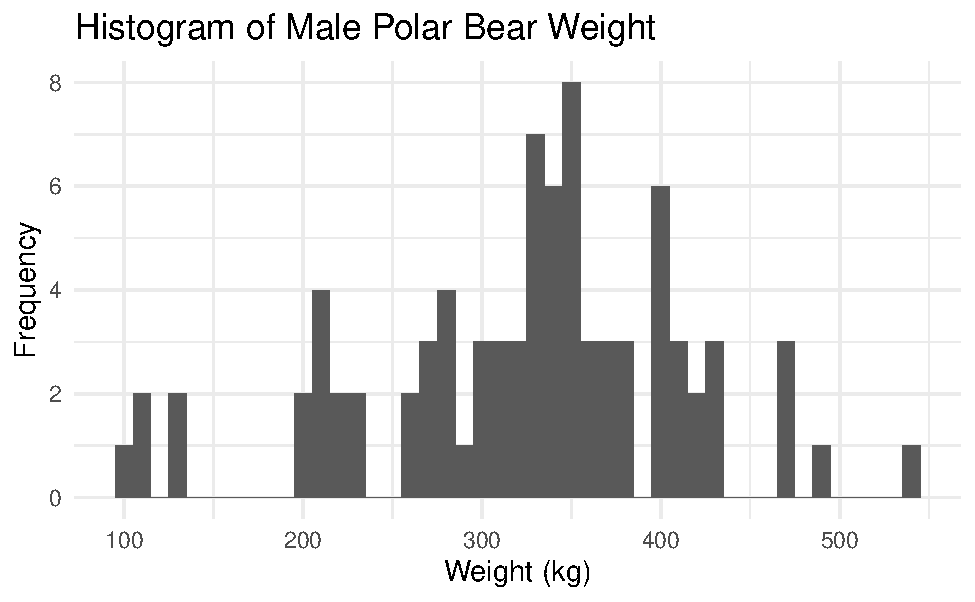
\includegraphics[width=0.6\linewidth]{06-VN06-EDAonemeanSim_files/figure-latex/unnamed-chunk-11-1} 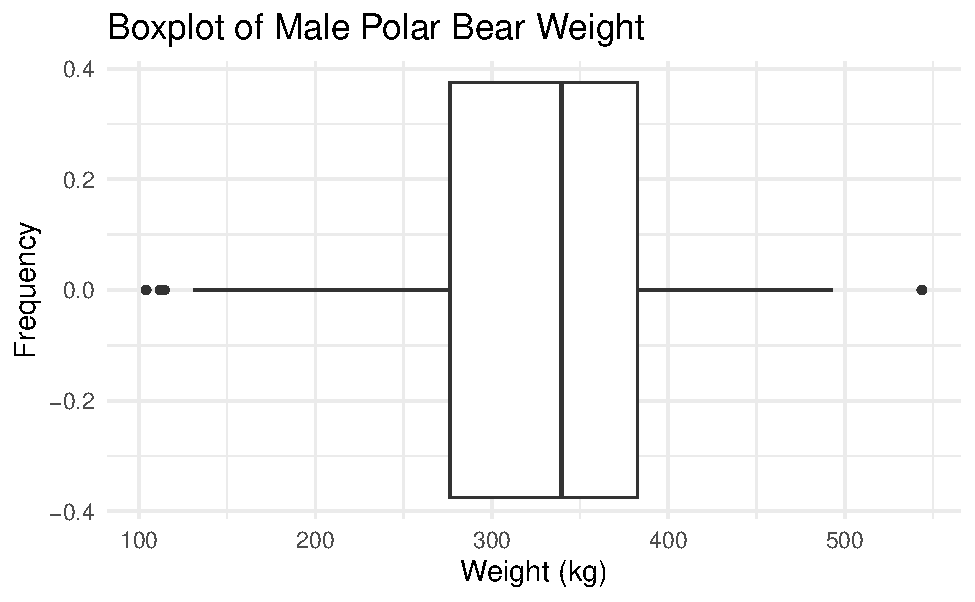
\includegraphics[width=0.6\linewidth]{06-VN06-EDAonemeanSim_files/figure-latex/unnamed-chunk-11-2} \end{center}

\newpage

Summary Statistics:

\begin{Shaded}
\begin{Highlighting}[]
\NormalTok{pb }\SpecialCharTok{\%\textgreater{}\%}
  \FunctionTok{summarise}\NormalTok{(}\FunctionTok{favstats}\NormalTok{(Weight)) }\CommentTok{\#Gives the summary statistics}
\CommentTok{\#\textgreater{}     min    Q1 median     Q3   max     mean       sd  n missing}
\CommentTok{\#\textgreater{} 1 104.1 276.3  339.4 382.45 543.6 324.5988 88.32615 83       0}
\end{Highlighting}
\end{Shaded}

\subsection*{Hypothesis testing}\label{hypothesis-testing-2}
\addcontentsline{toc}{subsection}{Hypothesis testing}

\setstretch{1.5}

\begin{itemize}
\tightlist
\item
  Hypotheses are always written about the \_\_\_\_\_\_\_\_\_\_\_\_\_\_\_\_\_\_\_\_\_\_\_\_\_. For a single mean we will use the notation \_\_\_\_\_\_\_\_\_\_\_.
\end{itemize}

\setstretch{1}

Null Hypothesis:

\(H_0:\)

\vspace{0.2in}

Alternative Hypothesis:

\(H_A:\)

\vspace{0.2in}

\setstretch{1.5}

\begin{itemize}
\tightlist
\item
  Direction of the alternative depends on the \_\_\_\_\_\_\_\_\_\_\_\_\_\_\_\_\_\_
  \_\_\_\_\_\_\_\_\_\_\_\_\_\_\_\_\_\_\_.
\end{itemize}

\setstretch{1}

\subsubsection*{Simulation-based method}\label{simulation-based-method-2}
\addcontentsline{toc}{subsubsection}{Simulation-based method}

\begin{itemize}
\item
  Simulate many samples assuming \(H_0: \mu = \mu_0\)

  \begin{itemize}
  \item
    Shift the data by the difference between \(\mu_0\) and \(\bar{x}\)
  \item
    Sample with replacement \(n\) times from the shifted data
  \item
    Plot the simulated shifted sample mean from each simulation
  \item
    Repeat 10000 times (simulations) to create the null distribution
  \item
    Find the proportion of simulations at least as extreme as \(\bar{x}\)
  \end{itemize}
\end{itemize}

Example: Is there evidence that male polar bears weigh less than 370kg (previously recorded measure), on average? The weight was measured on a representative sample of 83 male polar bears from the Southern Beaufort Sea.

Hypotheses:

In notation:

\(H_0:\)

\vspace{0.2in}

\(H_A:\)

\vspace{0.2in}

\newpage

In words:

\(H_0:\)

\vspace{0.6in}

\(H_A:\)

\vspace{0.6in}

Reminder of summary statistics:

\begin{Shaded}
\begin{Highlighting}[]
\NormalTok{pb }\SpecialCharTok{\%\textgreater{}\%}
  \FunctionTok{summarise}\NormalTok{(}\FunctionTok{favstats}\NormalTok{(Weight)) }\CommentTok{\#Gives the summary statistics}
\CommentTok{\#\textgreater{}     min    Q1 median     Q3   max     mean       sd  n missing}
\CommentTok{\#\textgreater{} 1 104.1 276.3  339.4 382.45 543.6 324.5988 88.32615 83       0}
\end{Highlighting}
\end{Shaded}

Find the difference:

\(\mu_0 - \bar{x} =\)

\begin{Shaded}
\begin{Highlighting}[]
\FunctionTok{set.seed}\NormalTok{(}\DecValTok{216}\NormalTok{)}
\FunctionTok{one\_mean\_test}\NormalTok{(pb}\SpecialCharTok{$}\NormalTok{Weight,   }\CommentTok{\#Enter the object name and variable}
              \AttributeTok{null\_value =} \DecValTok{370}\NormalTok{, }\CommentTok{\#Enter null value for the study}
              \AttributeTok{summary\_measure =} \StringTok{"mean"}\NormalTok{,  }\CommentTok{\#Can choose between mean or median}
              \AttributeTok{shift =} \FloatTok{45.4}\NormalTok{,   }\CommentTok{\# Shift needed for bootstrap hypothesis test}
              \AttributeTok{as\_extreme\_as =} \FloatTok{324.6}\NormalTok{,  }\CommentTok{\# Observed statistic}
              \AttributeTok{direction =} \StringTok{"less"}\NormalTok{,  }\CommentTok{\# Direction of alternative}
              \AttributeTok{number\_repetitions =} \DecValTok{10000}\NormalTok{)  }\CommentTok{\# Number of simulated samples for null distribution}
\end{Highlighting}
\end{Shaded}

\begin{center}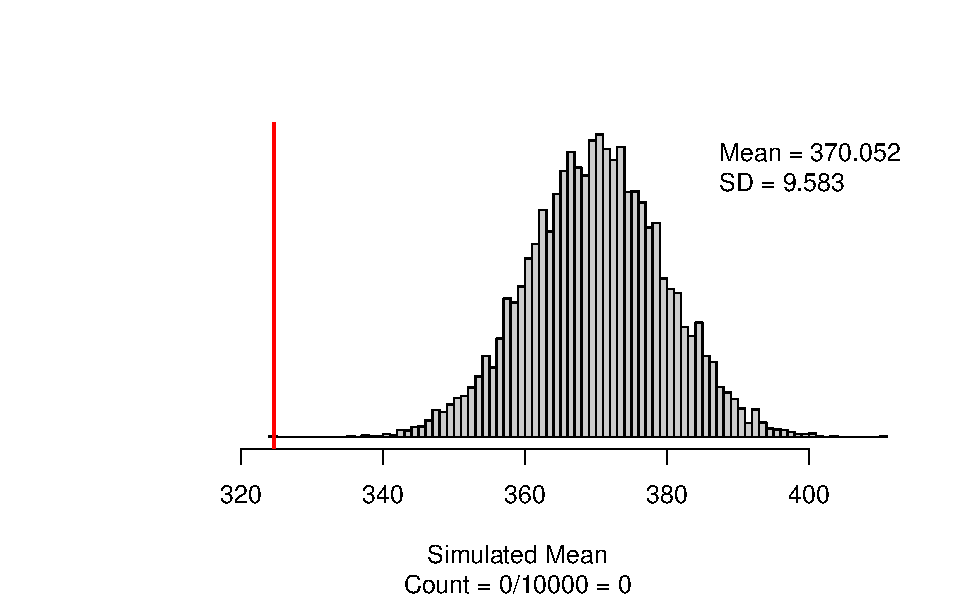
\includegraphics[width=0.6\linewidth]{06-VN06-EDAonemeanSim_files/figure-latex/unnamed-chunk-14-1} \end{center}

\newpage

Interpretation of the p-value:

\begin{itemize}
\item
  Statement about probability or proportion of samples
\item
  Statistic (summary measure and value)
\item
  Direction of the alternative
\item
  Null hypothesis (in context)
\end{itemize}

\vspace{0.8in}

Conclusion:

\begin{itemize}
\item
  Amount of evidence
\item
  Parameter of interest
\item
  Direction of the alternative hypothesis
\end{itemize}

\vspace{0.8in}

\subsubsection*{Theory-based method}\label{theory-based-method-1}
\addcontentsline{toc}{subsubsection}{Theory-based method}

Conditions for inference using theory-based methods:

\begin{itemize}
\tightlist
\item
  Independence:
\end{itemize}

\vspace{0.2in}

\begin{itemize}
\tightlist
\item
  Large enough sample size:
\end{itemize}

\vspace{0.2in}

\subsection*{\texorpdfstring{\(t\)-distribution}{t-distribution}}\label{t-distribution}
\addcontentsline{toc}{subsection}{\(t\)-distribution}

In the theoretical approach, we use the Central Limit Theorem (CLT) to tell us that---under certain conditions---the distribution of sample means will be approximately normal, centered at the assumed true mean under \(H_0\), and with standard deviation \(\frac{\sigma}{\sqrt{n}}\).

\[\bar{x} \sim N\left(\mu_0, \frac{\sigma}{\sqrt{n}}\right)\]
\setstretch{1.5}

\begin{itemize}
\item
  Estimate the population standard deviation, \(\sigma\), with the
  \_\_\_\_\_\_\_\_\_\_\_\_\_\_\_\_\_\_\_\_\_\_\_\_\_\_\_ standard deviation, \_\_\_\_\_\_\_\_.
\item
  For a single quantitative variable we use the \_\_\_\_ - distribution
  with \_\_\_\_\_\_\_\_\_\_\_\_\_\_\_
  degrees of freedom to approximate the sampling distribution.
\end{itemize}

\setstretch{1}

The \(t^*\) multiplier is the value at the given percentile of the \(t\)-distribution with \(n - 1\) degrees of freedom.

\begin{center}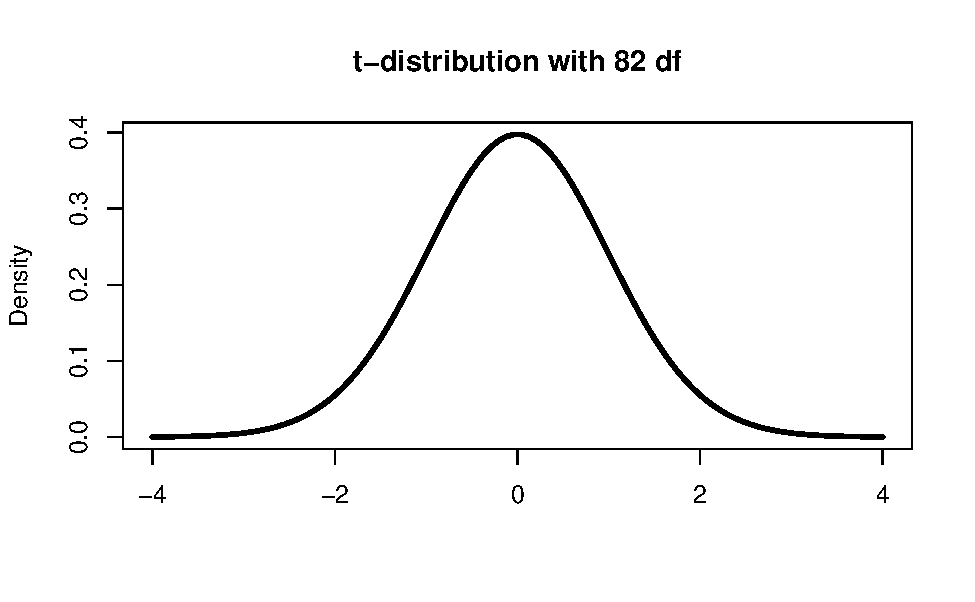
\includegraphics[width=0.7\linewidth]{06-VN06-EDAonemeanSim_files/figure-latex/tstarpb-1} \end{center}

\begin{itemize}
\item
  Calculate the standardized statistic
\item
  Find the area under the \(t\)-distribution with \(n - 1\) df at least as extreme as the standardized statistic
\end{itemize}

Equation for the standard error of the sample mean:

\vspace{0.5in}

Equation for the standardized sample mean:

\vspace{0.5in}

Calculate the standardized sample mean weight of adult male polar bears:

\vspace{0.4in}

\begin{center}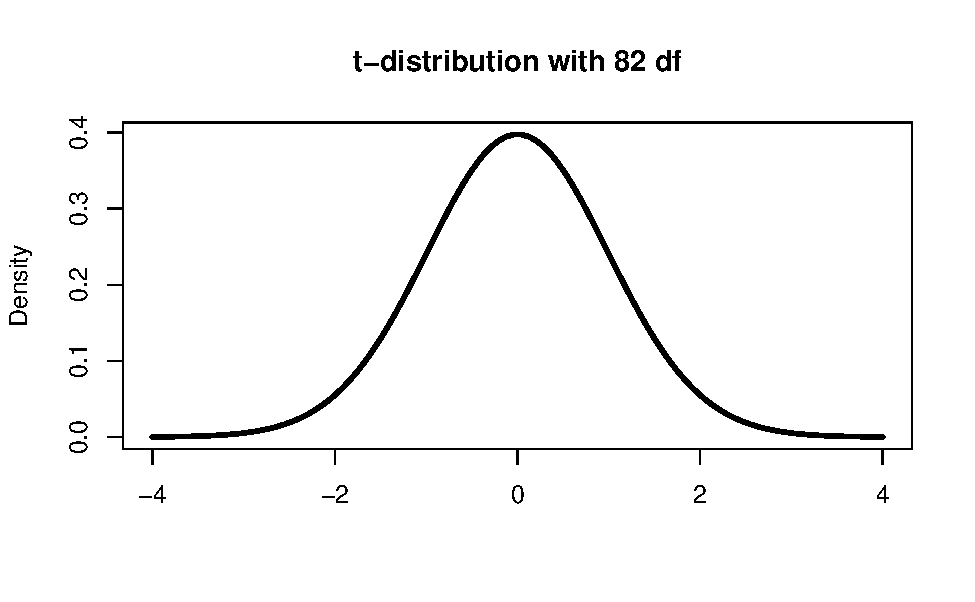
\includegraphics[width=0.7\linewidth]{06-VN06-EDAonemeanSim_files/figure-latex/pvaluepb-1} \end{center}

Interpret the standardized sample mean weight:

\vspace{0.8in}

To find the theory-based p-value:

\begin{Shaded}
\begin{Highlighting}[]
\FunctionTok{pt}\NormalTok{(}\SpecialCharTok{{-}}\FloatTok{4.683}\NormalTok{, }\AttributeTok{df=}\DecValTok{82}\NormalTok{, }\AttributeTok{lower.tail=}\ConstantTok{TRUE}\NormalTok{)}
\CommentTok{\#\textgreater{} [1] 5.531605e{-}06}
\end{Highlighting}
\end{Shaded}

\subsection{Concept Check}\label{concept-check-5}

Be prepared for group discussion in the next class. One member from the table should write the answers to the following on the whiteboard.

\begin{enumerate}
\def\labelenumi{\arabic{enumi}.}
\tightlist
\item
  What plots can be used to summarize quantitative data?
\end{enumerate}

\vspace{0.7in}

\begin{enumerate}
\def\labelenumi{\arabic{enumi}.}
\setcounter{enumi}{1}
\tightlist
\item
  Which measure of center is robust to outliers?
\end{enumerate}

\vspace{0.2in}

\begin{enumerate}
\def\labelenumi{\arabic{enumi}.}
\setcounter{enumi}{2}
\tightlist
\item
  How do we determine the direction of the alternative hypothesis?
\end{enumerate}

\newpage

\section{Activity 11: Summarizing Quantitative Variables}\label{activity-11-summarizing-quantitative-variables}

\setstretch{1}

\subsection{Learning outcomes}\label{learning-outcomes-11}

\begin{itemize}
\item
  Identify and create appropriate summary statistics and plots given a data set or research question for quantitative data.
\item
  Interpret the following summary statistics in context:
  median, lower quartile, upper quartile,
  standard deviation, interquartile range.
\end{itemize}

\subsection{Terminology review}\label{terminology-review-9}

In today's activity, we will review summary measures and plots for quantitative variables. Some terms covered in this activity are:

\begin{itemize}
\item
  Two measures of center: mean, median
\item
  Two measures of spread (variability): standard deviation, interquartile range (IQR)
\item
  Plots of quantitative variables: dotplots, boxplots, histograms
\item
  Given a plot or set of plots, describe and compare the distribution(s)
  of quantitative variables
  (center, variability, shape, outliers).
\end{itemize}

To review these concepts, see Chapter 5 in the textbook.

\subsection{The Integrated Postsecondary Education Data System (IPEDS)}\label{the-integrated-postsecondary-education-data-system-ipeds}

These data were collected on a subset of higher education institutions that met the following selection criteria (Education Statistics 2018):

\begin{itemize}
\item
  Degree granting
\item
  United States only
\item
  Title IV participating
\item
  Not for profit
\item
  2-year or 4-year or above
\item
  Has full-time first-time undergraduates
\end{itemize}

Some of the variables collected and their descriptions are below. Note that several variables have missing values for some institutions (denoted by ``NA'').

\begin{longtable}[]{@{}
  >{\raggedright\arraybackslash}p{(\columnwidth - 2\tabcolsep) * \real{0.2353}}
  >{\raggedright\arraybackslash}p{(\columnwidth - 2\tabcolsep) * \real{0.7647}}@{}}
\toprule\noalign{}
\begin{minipage}[b]{\linewidth}\raggedright
\textbf{Variable}
\end{minipage} & \begin{minipage}[b]{\linewidth}\raggedright
\textbf{Description}
\end{minipage} \\
\midrule\noalign{}
\endhead
\bottomrule\noalign{}
\endlastfoot
\texttt{UnitID} & Unique institution identifier \\
\texttt{Name} & Institution name \\
\texttt{State} & State abbreviation \\
\texttt{Sector} & whether public or private \\
\texttt{LandGrant} & Is this a land-grant institution (Yes/No) \\
\texttt{Size} & Institution size category based on total student enrolled for credit, Fall 2018: Under 1,000, 1,000\$-\(4,999, 5,000\)-\(9,999, 10,000\)-\$19,999, 20,000 and above \\
\texttt{Cost\_OutofState} & Cost of attendance for full-time out-of-state undergraduate students \\
\texttt{Cost\_InState} & Cost of attendance for full-time in-state undergraduate students \\
\texttt{Retention} & Retention rate is the percent of the undergraduate students that re-enroll in the next year \\
\texttt{Graduation\_Rate} & 6-year graduation rate for undergraduate students \\
\texttt{SATMath\_75} & 75th percentile Math SAT score \\
\texttt{ACT\_75} & 75th percentile ACT score \\
\end{longtable}

\subsubsection*{Identifying variables in a data set}\label{identifying-variables-in-a-data-set}
\addcontentsline{toc}{subsubsection}{Identifying variables in a data set}

Look through the provided table of variable descriptions. The \texttt{UnitID} and \texttt{Name} are identifiers for each observational unit, \emph{US degree-granting higher education institutions in 2018}.

\begin{enumerate}
\def\labelenumi{\arabic{enumi}.}
\tightlist
\item
  Identify in the table which variables collected on the US institutions are categorical (C) and which variables are quantitative (Q).
\end{enumerate}

\subsubsection*{Summarizing quantitative variables}\label{summarizing-quantitative-variables}
\addcontentsline{toc}{subsubsection}{Summarizing quantitative variables}

The \texttt{favstats()} function from the \texttt{mosaic} package gives the summary statistics for a quantitative variable. The \texttt{R} output below provides the summary statistics for the variable \texttt{Graduation\_Rate}. The summary statistics provided are the two measures of center (mean and median) and two measures of spread (standard deviation and the quartile values to calculate the IQR) for undergraduate 6-year graduation rate.

\begin{itemize}
\item
  Highlight and run lines 1--12 in the provided \texttt{R} script file to load the data set. Check that the summary statistics match the output given in the coursepack.
\item
  Notice that the 2-year institutions were removed so the observational units for this study are \textbf{4-year US degree-granting higher education institutions in 2018.}
\end{itemize}

\begin{Shaded}
\begin{Highlighting}[]
\NormalTok{IPEDS }\OtherTok{\textless{}{-}} \FunctionTok{read.csv}\NormalTok{(}\StringTok{"https://www.math.montana.edu/courses/s216/data/IPEDS\_2018.csv"}\NormalTok{) }
\NormalTok{IPEDS }\OtherTok{\textless{}{-}}\NormalTok{ IPEDS }\SpecialCharTok{\%\textgreater{}\%}
  \FunctionTok{filter}\NormalTok{(Sector }\SpecialCharTok{!=} \StringTok{"Public 2{-}year"}\NormalTok{) }\CommentTok{\# Filters the data set to remove Public 2{-}year}
\NormalTok{IPEDS }\OtherTok{\textless{}{-}}\NormalTok{ IPEDS }\SpecialCharTok{\%\textgreater{}\%}
  \FunctionTok{filter}\NormalTok{(Sector }\SpecialCharTok{!=} \StringTok{"Private 2{-}year"}\NormalTok{) }\CommentTok{\# Filters the data set to remove Private 2{-}year}
\NormalTok{IPEDS }\SpecialCharTok{\%\textgreater{}\%}
    \FunctionTok{summarize}\NormalTok{(}\FunctionTok{favstats}\NormalTok{(Graduation\_Rate))}
\end{Highlighting}
\end{Shaded}

\begin{verbatim}
#>   min Q1 median Q3 max     mean       sd    n missing
#> 1   0 38     53 67 100 52.48749 20.63192 1918      49
\end{verbatim}

\begin{enumerate}
\def\labelenumi{\arabic{enumi}.}
\setcounter{enumi}{1}
\tightlist
\item
  Report the values for the two measures of center (mean and median).
\end{enumerate}

\vspace{0.5in}

\begin{enumerate}
\def\labelenumi{\arabic{enumi}.}
\setcounter{enumi}{2}
\tightlist
\item
  Calculate the interquartile range (\(IQR = Q_3 - Q_1\)) of graduation rates.
\end{enumerate}

\vspace{0.5in}

\begin{enumerate}
\def\labelenumi{\arabic{enumi}.}
\setcounter{enumi}{3}
\item
  Report the value of the standard deviation and interpret this value in context of the problem.
  \vspace{0.8in}
\item
  Interpret the value of \(Q_3\) in context of the study.
\end{enumerate}

\vspace{0.8in}

\subsubsection*{Displaying a single quantitative variable}\label{displaying-a-single-quantitative-variable}
\addcontentsline{toc}{subsubsection}{Displaying a single quantitative variable}

There are three type of plots used to plot a single quantitative variable: a dotplot, a histogram or a boxplot. A dotplot of graduation rates would plot a dot for the graduation rate for each 4-year US higher education institution.

First, let's create a histogram of the variable \texttt{Graduation\_Rate}.

\begin{itemize}
\item
  Enter the name of the variable in line 19 for \texttt{variable} in the R script file.
\item
  Replace the word title for the plot in line 21 between the quotations with a descriptive title. \textbf{A title should include: type of plot, variable or variables plotted, and observational units.}
\item
  Highlight and run lines 18--23 to create the histogram.
\end{itemize}

\begin{Shaded}
\begin{Highlighting}[]
\NormalTok{IPEDS }\SpecialCharTok{\%\textgreater{}\%} \CommentTok{\# Data set piped into...}
\FunctionTok{ggplot}\NormalTok{(}\FunctionTok{aes}\NormalTok{(}\AttributeTok{x =}\NormalTok{ xx)) }\SpecialCharTok{+}   \CommentTok{\# Name variable to plot}
  \FunctionTok{geom\_histogram}\NormalTok{(}\AttributeTok{binwidth =} \DecValTok{10}\NormalTok{) }\SpecialCharTok{+}  \CommentTok{\# Create histogram with specified binwidth}
  \FunctionTok{labs}\NormalTok{(}\AttributeTok{title =} \StringTok{"Don\textquotesingle{}t forget to title the plot!"}\NormalTok{, }\CommentTok{\# Title for plot}
       \AttributeTok{x =} \StringTok{"Graduation Rate"}\NormalTok{, }\CommentTok{\# Label for x axis}
       \AttributeTok{y =} \StringTok{"Frequency"}\NormalTok{) }\CommentTok{\# Label for y axis}
\end{Highlighting}
\end{Shaded}

Notice that the \textbf{bin width} for the histogram is 10. For example the first bin consists of the number of institutions in the data set with a graduation rate of 0 to 10\%. It is important to note that a graduation rate on the boundary of a bin will fall into the bin above it; for example, 20 would be counted in the bin 20--30.

\begin{enumerate}
\def\labelenumi{\arabic{enumi}.}
\setcounter{enumi}{5}
\tightlist
\item
  Which range of Graduation Rates have the highest frequency?
\end{enumerate}

\vspace{0.3in}

Next we will create a boxplot of the variable \texttt{Graduation\_Rate}.

\begin{itemize}
\item
  Enter the name of the variable in line 28 for \texttt{variable} in the R script file.
\item
  Highlight and run lines 28--36 to create the boxplot.
\end{itemize}

\begin{Shaded}
\begin{Highlighting}[]
\NormalTok{IPEDS }\SpecialCharTok{\%\textgreater{}\%} \CommentTok{\# Data set piped into...}
\FunctionTok{ggplot}\NormalTok{(}\FunctionTok{aes}\NormalTok{(}\AttributeTok{x =}\NormalTok{ variable)) }\SpecialCharTok{+}   \CommentTok{\# Name variable to plot}
  \FunctionTok{geom\_boxplot}\NormalTok{() }\SpecialCharTok{+}  \CommentTok{\# Create boxplot with specified binwidth}
  \FunctionTok{labs}\NormalTok{(}\AttributeTok{title =} \StringTok{"Boxplot of Graduation Rates for }\SpecialCharTok{\textbackslash{}n}\StringTok{ 4{-}year Higher Education Institutions"}\NormalTok{, }
           \CommentTok{\# Title for plot}
           \CommentTok{\# Note the \textbackslash{}n starts a new line}
       \AttributeTok{x =} \StringTok{"Graduation\_Rate"}\NormalTok{, }\CommentTok{\# Label for x axis}
       \AttributeTok{y =} \StringTok{""}\NormalTok{) }\SpecialCharTok{+} \CommentTok{\# Remove y axis label}
    \FunctionTok{theme}\NormalTok{(}\AttributeTok{axis.text.y =} \FunctionTok{element\_blank}\NormalTok{(), }
          \AttributeTok{axis.ticks.y =} \FunctionTok{element\_blank}\NormalTok{()) }\CommentTok{\# Removes y{-}axis ticks}
\end{Highlighting}
\end{Shaded}

\begin{enumerate}
\def\labelenumi{\arabic{enumi}.}
\setcounter{enumi}{6}
\tightlist
\item
  Sketch the boxplot created and identify the values of the 5-number summary (minimum value, \(Q_1\), median, \(Q_3\), maximum value) on the plot. Use the following formulas to find the invisible fence on both ends of the distribution. Draw a dotted line at the invisible fence to show how the outliers were detected (any values less than the lower fence or greater than the upper fence were flagged as outliers).
\end{enumerate}

\[\text{Lower Fence:} ~~~ Q_1 - 1.5\times IQR~~~~~~~\text{Upper Fence:} ~~~ Q_3 + 1.5\times IQR\]
\vspace{1.8in}

When describing distributions of quantitative variables we discuss the \textbf{shape} (symmetric or skewed), the \textbf{center} (mean or median), \textbf{spread} (standard deviation or IQR), and if there are \textbf{outliers} present.

\begin{enumerate}
\def\labelenumi{\arabic{enumi}.}
\setcounter{enumi}{7}
\tightlist
\item
  What is the shape of the distribution of graduation rates?
\end{enumerate}

\vspace{0.4in}

\begin{enumerate}
\def\labelenumi{\arabic{enumi}.}
\setcounter{enumi}{8}
\tightlist
\item
  From which plot (histogram or boxplot) is it easier to determine the shape of the distribution?
\end{enumerate}

\vspace{0.3in}

\begin{enumerate}
\def\labelenumi{\arabic{enumi}.}
\setcounter{enumi}{9}
\tightlist
\item
  From which plot is it easier to determine if there are outliers?
\end{enumerate}

\vspace{0.3in}

\subsubsection*{Robust statistics}\label{robust-statistics}
\addcontentsline{toc}{subsubsection}{Robust statistics}

Let's examine how the presence of outliers affects the different summary measures for center and spread. For this part of the activity, we will look at the retention rate variable (\texttt{Retention}) in the IPEDS data set.

\begin{Shaded}
\begin{Highlighting}[]
\NormalTok{IPEDS }\SpecialCharTok{\%\textgreater{}\%} \CommentTok{\# Data set piped into...}
    \FunctionTok{summarise}\NormalTok{(}\FunctionTok{favstats}\NormalTok{(Retention))}
\CommentTok{\#\textgreater{}   min Q1 median Q3 max    mean       sd    n missing}
\CommentTok{\#\textgreater{} 1   0 66     75 83 100 73.8525 15.14323 1817     150}

\NormalTok{IPEDS }\SpecialCharTok{\%\textgreater{}\%} \CommentTok{\# Data set piped into...}
    \FunctionTok{ggplot}\NormalTok{(}\FunctionTok{aes}\NormalTok{(}\AttributeTok{x =}\NormalTok{ Retention)) }\SpecialCharTok{+} \CommentTok{\# Name variable to plot}
    \FunctionTok{geom\_boxplot}\NormalTok{() }\SpecialCharTok{+} \CommentTok{\# Create boxplot }
    \FunctionTok{labs}\NormalTok{(}\AttributeTok{title =} \StringTok{"Boxplot of Retention Rates for }\SpecialCharTok{\textbackslash{}n}\StringTok{ 4{-}year Higher Education Institutions"}\NormalTok{,}
           \CommentTok{\# Title for plot}
         \AttributeTok{x =} \StringTok{"Retention Rates (\%)"}\NormalTok{, }\CommentTok{\# Label for x axis}
         \AttributeTok{y =} \StringTok{"Frequency"}\NormalTok{) }\CommentTok{\# Label for y axis}
\end{Highlighting}
\end{Shaded}

\begin{center}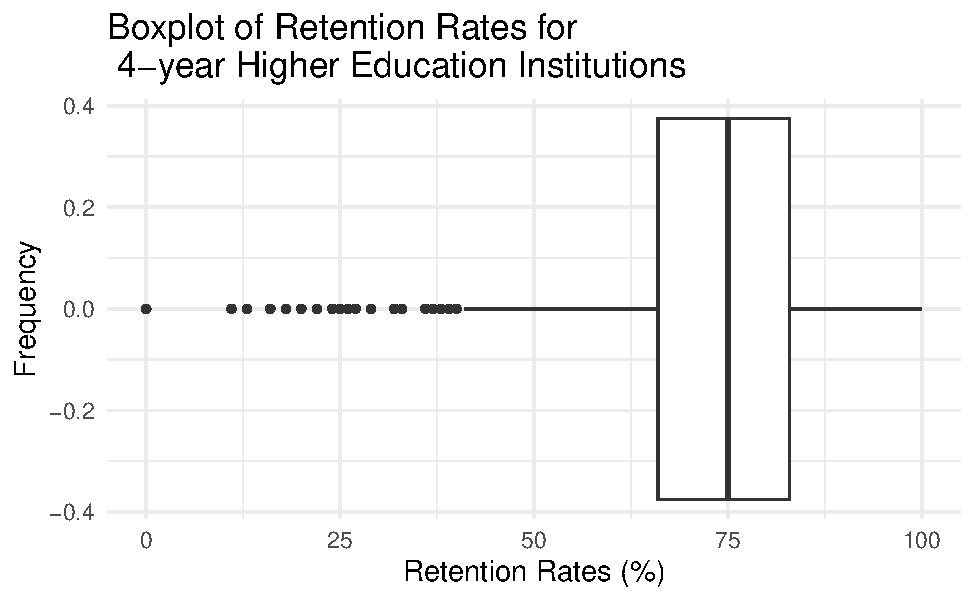
\includegraphics[width=0.7\linewidth]{06-A11-EDA-quantitative_files/figure-latex/unnamed-chunk-4-1} \end{center}

\begin{enumerate}
\def\labelenumi{\arabic{enumi}.}
\setcounter{enumi}{10}
\tightlist
\item
  Report the values for the two measures of center for these data.
\end{enumerate}

\vspace{0.5in}

\begin{enumerate}
\def\labelenumi{\arabic{enumi}.}
\setcounter{enumi}{11}
\tightlist
\item
  Report the values for the two measures of spread for these data.
\end{enumerate}

\vspace{0.5in}

To show the effect of outliers on the measures of center and spread, the smallest values of retention rate in the
data set were increased by 30\%. This variable is called \texttt{Retention\_Inc}.

\begin{Shaded}
\begin{Highlighting}[]
\NormalTok{IPEDS }\SpecialCharTok{\%\textgreater{}\%} \CommentTok{\# Data set piped into...}
    \FunctionTok{summarise}\NormalTok{(}\FunctionTok{favstats}\NormalTok{(Retention\_Inc))}
\CommentTok{\#\textgreater{}   min Q1 median Q3 max     mean       sd    n missing}
\CommentTok{\#\textgreater{} 1  30 66     75 83 100 74.49642 13.41255 1817     150}

\NormalTok{IPEDS }\SpecialCharTok{\%\textgreater{}\%} \CommentTok{\# Data set piped into...}
    \FunctionTok{ggplot}\NormalTok{(}\FunctionTok{aes}\NormalTok{(}\AttributeTok{x =}\NormalTok{ Retention\_Inc)) }\SpecialCharTok{+} \CommentTok{\# Name variable to plot}
    \FunctionTok{geom\_boxplot}\NormalTok{() }\SpecialCharTok{+} \CommentTok{\# Create histogram }
    \FunctionTok{labs}\NormalTok{(}\AttributeTok{title =} \StringTok{"Boxplot of Increased Retention Rates for }\SpecialCharTok{\textbackslash{}n}\StringTok{ 4{-}year Higher Education Institutions"}\NormalTok{, }
        \CommentTok{\# Title for plot}
        \AttributeTok{x =} \StringTok{"Retention Rates (\%)"}\NormalTok{, }\CommentTok{\# Label for x axis}
        \AttributeTok{y =} \StringTok{"Frequency"}\NormalTok{) }\CommentTok{\# Label for y axis}
\end{Highlighting}
\end{Shaded}

\begin{center}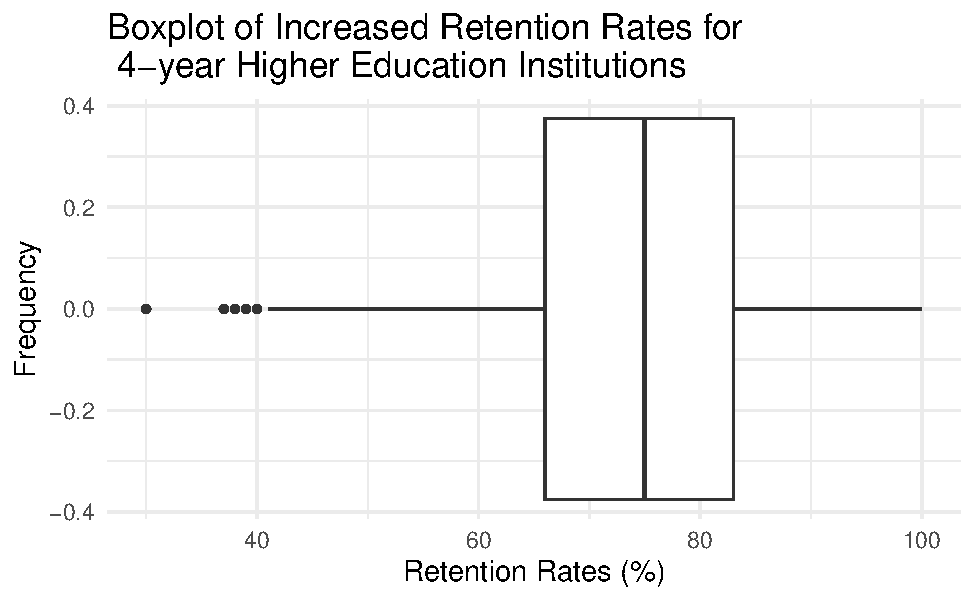
\includegraphics[width=0.7\linewidth]{06-A11-EDA-quantitative_files/figure-latex/unnamed-chunk-5-1} \end{center}

\begin{enumerate}
\def\labelenumi{\arabic{enumi}.}
\setcounter{enumi}{12}
\item
  Report the values for the two measures of center for this new data set.
  \vspace{0.5in}
\item
  Report the values for the two measures of spread for this new data set.
  \vspace{0.5in}
\item
  Which measure of center is robust to outliers? Explain your answer.
  \vspace{0.8in}
\item
  Which measure of spread is robust to outliers? Explain your answer.
  \vspace{0.8in}
\end{enumerate}

\subsection{Take-home messages}\label{take-home-messages-10}

\begin{enumerate}
\def\labelenumi{\arabic{enumi}.}
\item
  Histograms, box plots, and dot plots can all be used to graphically display a single quantitative variable.
\item
  The box plot is created using the five number summary: minimum value, quartile 1, median, quartile 3, and maximum value. Whiskers extend to the lowest value and highest value that are \emph{not} considered outliers. Values in the data set that are less than \(Q_1 - 1.5\times IQR\) or greater than \(Q_3 + 1.5\times IQR\) are considered outliers and are graphically represented by a dot outside of the whiskers on the box plot.
\item
  Data should be summarized numerically and displayed graphically to give us information about the study.
\item
  When comparing distributions of quantitative variables we look at the shape, center, spread, and for outliers. In this course, we only consider two measures of center (mean and the median), and two measures of spread (standard deviation and the interquartile range, \(IQR = Q_3 - Q_1\)).
\end{enumerate}

\subsection{Additional notes}\label{additional-notes-10}

Use this space to summarize your thoughts and take additional notes on today's activity and material covered.

\newpage

\section{Activity 12: Hypothesis Testing of a Single Quantitative Variable}\label{activity-12-hypothesis-testing-of-a-single-quantitative-variable}

\setstretch{1}

\subsection{Learning outcomes}\label{learning-outcomes-12}

\begin{itemize}
\item
  Given a research question involving one quantitative variable, construct the null and alternative hypotheses
  in words and using appropriate statistical symbols.
\item
  Investigate the process of creating a null distribution for one quantitative variable.
\item
  Find, evaluate, and interpret a p-value from the null distribution.
\end{itemize}

\subsection{Terminology review}\label{terminology-review-10}

In today's activity, we will use simulation-based and theory-based methods to analyze a single quantitative variable. Some terms covered in this activity are:

\begin{itemize}
\item
  Null hypothesis
\item
  Alternative hypothesis
\item
  Null distribution
\item
  \(t\)-distribution
\item
  p-value
\end{itemize}

To review these concepts, see Chapters 9 and 17 in the textbook.

\subsection{College student sleep habits}\label{college-student-sleep-habits}

According to an article in \emph{Sleep} (Watson 2015), experts recommend adults (\textgreater18 years old) get at least 7 hours of sleep per night. A professor at MSU is interested in the sleep habits of MSU students. The professor obtained a representative sample of MSU students and asked each student to report the amount of sleep they get on a typically night. Is there evidence that MSU students get less than the recommended 7 hours of sleep per night, on average?

\subsubsection*{Summarizing quantitative variables}\label{summarizing-quantitative-variables-1}
\addcontentsline{toc}{subsubsection}{Summarizing quantitative variables}

\begin{itemize}
\item
  Download the R script file and data file for this activity
\item
  Upload both files to the RStudio server and open the R script file
\item
  Enter the name of the dataset for datasetname.csv
\item
  Highlight and run lines 1--8 to load the data
\end{itemize}

\begin{Shaded}
\begin{Highlighting}[]
\NormalTok{sleep }\OtherTok{\textless{}{-}} \FunctionTok{read.csv}\NormalTok{(}\StringTok{"datasetname.csv"}\NormalTok{)}
\end{Highlighting}
\end{Shaded}

\subsubsection*{Ask a research question}\label{ask-a-research-question-1}
\addcontentsline{toc}{subsubsection}{Ask a research question}

\begin{enumerate}
\def\labelenumi{\arabic{enumi}.}
\tightlist
\item
  Write the parameter of interest in context of the study.
\end{enumerate}

\vspace{1in}

\begin{enumerate}
\def\labelenumi{\arabic{enumi}.}
\setcounter{enumi}{1}
\tightlist
\item
  Write the null hypothesis in words in context of the study.
\end{enumerate}

\vspace{1in}

\begin{enumerate}
\def\labelenumi{\arabic{enumi}.}
\setcounter{enumi}{2}
\tightlist
\item
  Write the alternative hypothesis in notation.
\end{enumerate}

\vspace{0.4in}

\subsubsection*{Summarize and visualize the data}\label{summarize-and-visualize-the-data-1}
\addcontentsline{toc}{subsubsection}{Summarize and visualize the data}

The \texttt{favstats()} function from the \texttt{mosaic} package gives the summary statistics for a quantitative variable.

\begin{itemize}
\item
  Enter the variable name, \texttt{SleepHours}, for \texttt{variable} in line 13
\item
  Highlight and run lines 12--13
\end{itemize}

\begin{Shaded}
\begin{Highlighting}[]
\NormalTok{sleep }\SpecialCharTok{\%\textgreater{}\%}
    \FunctionTok{summarize}\NormalTok{(}\FunctionTok{favstats}\NormalTok{(variable))}
\end{Highlighting}
\end{Shaded}

\begin{enumerate}
\def\labelenumi{\arabic{enumi}.}
\setcounter{enumi}{3}
\tightlist
\item
  About how far is each number of hours of sleep for a Stat 216 student from the mean number of hours of sleep, on average?
\end{enumerate}

\vspace{0.3in}

Create a boxplot of the variable \texttt{SleepHours}.

\begin{itemize}
\item
  Enter the name of the variable in line 19 for \texttt{variable} in the R script file.
\item
  Enter a title in line 21 for the plot between the quotations.
\item
  Highlight and run lines 18--25.
\end{itemize}

\begin{Shaded}
\begin{Highlighting}[]
\NormalTok{sleep }\SpecialCharTok{\%\textgreater{}\%} \CommentTok{\# Data set piped into...}
    \FunctionTok{ggplot}\NormalTok{(}\FunctionTok{aes}\NormalTok{(}\AttributeTok{x =}\NormalTok{ variable)) }\SpecialCharTok{+}   \CommentTok{\# Name variable to plot}
    \FunctionTok{geom\_boxplot}\NormalTok{() }\SpecialCharTok{+}  \CommentTok{\# Create boxplot with specified binwidth}
    \FunctionTok{labs}\NormalTok{(}\AttributeTok{title =} \StringTok{"Don\textquotesingle{}t forget to title your plot!"}\NormalTok{, }\CommentTok{\# Title for plot}
       \AttributeTok{x =} \StringTok{"Amount of sleep (hrs)"}\NormalTok{, }\CommentTok{\# Label for x axis}
       \AttributeTok{y =} \StringTok{""}\NormalTok{) }\SpecialCharTok{+} \CommentTok{\# Remove y axis label}
    \FunctionTok{theme}\NormalTok{(}\AttributeTok{axis.text.y =} \FunctionTok{element\_blank}\NormalTok{(), }
          \AttributeTok{axis.ticks.y =} \FunctionTok{element\_blank}\NormalTok{()) }\CommentTok{\# Removes y{-}axis ticks}
\end{Highlighting}
\end{Shaded}

\begin{enumerate}
\def\labelenumi{\arabic{enumi}.}
\setcounter{enumi}{4}
\tightlist
\item
  Describe the distribution of number of hours of sleep using the four characteristics of boxplots.
\end{enumerate}

\vspace{1in}

\subsection*{Simulation methods}\label{simulation-methods}
\addcontentsline{toc}{subsection}{Simulation methods}

To simulate the null distribution of sample means we will use a bootstrapping method. Recall that the null distribution must be created under the assumption that the null hypothesis is true. Therefore, before bootstrapping, we will need to \emph{shift} each data point by the difference \(\mu_0 - \bar{x}\). This will ensure that the mean of the shifted data is \(\mu_0\) (rather than the mean of the original data, \(\bar{x}\)), and that the simulated null distribution will be centered at the null value.

\begin{enumerate}
\def\labelenumi{\arabic{enumi}.}
\setcounter{enumi}{5}
\tightlist
\item
  Calculate the difference \(\mu_0 - \bar{x}\). Based on the sign of this difference, will we need to shift the data up or down?
\end{enumerate}

\newpage

\begin{itemize}
\item
  Open the data set (\texttt{sleep\_college}) in Excel.
\item
  Create a new column labeled Shift.
\item
  In the column, Shift, add the shifted value (answer to Q6) to each value in the \texttt{SleepHours} column.
\item
  Save the file and upload again to the RStudio server.
\item
  Find the \texttt{favstats} of the variable, \texttt{Shift}.
\item
  Highlight and run lines 30--32
\end{itemize}

\begin{Shaded}
\begin{Highlighting}[]
\NormalTok{sleep }\OtherTok{\textless{}{-}} \FunctionTok{read.csv}\NormalTok{(}\StringTok{"sleep\_college.csv"}\NormalTok{)}
\NormalTok{sleep }\SpecialCharTok{\%\textgreater{}\%}
    \FunctionTok{summarize}\NormalTok{(}\FunctionTok{favstats}\NormalTok{(Shift))}
\end{Highlighting}
\end{Shaded}

\begin{enumerate}
\def\labelenumi{\arabic{enumi}.}
\setcounter{enumi}{6}
\tightlist
\item
  Report the mean of the \texttt{Shift} variable. Why does it make sense that this value is the same as the null value?
\end{enumerate}

\vspace{0.9in}

\begin{enumerate}
\def\labelenumi{\arabic{enumi}.}
\setcounter{enumi}{7}
\tightlist
\item
  Report the standard deviation of the \texttt{Shift} variable. How does this compare to the standard deviation for the variable \texttt{SleepHours}? Explain why these values are the same.
\end{enumerate}

\vspace{0.9in}

\begin{enumerate}
\def\labelenumi{\arabic{enumi}.}
\setcounter{enumi}{8}
\tightlist
\item
  What inputs should be entered for each of the following to create the simulated null distribution?
  \vspace{1mm}
\end{enumerate}

\begin{itemize}
\tightlist
\item
  Null value (What is the null value for the study?):
\end{itemize}

\vspace{.15in}

\begin{itemize}
\tightlist
\item
  Summary measure (``mean'' or ``median''):
\end{itemize}

\vspace{0.15in}

\begin{itemize}
\tightlist
\item
  Shift (difference between \(\mu_0 -\bar{x}\)):
\end{itemize}

\vspace{0.15in}

\begin{itemize}
\tightlist
\item
  As extreme as (enter the value for the observed sample mean):
\end{itemize}

\vspace{.15in}

\begin{itemize}
\tightlist
\item
  Direction (\texttt{"greater"}, \texttt{"less"}, or \texttt{"two-sided"}):
\end{itemize}

\vspace{.15in}

\begin{itemize}
\tightlist
\item
  Number of repetitions:
\end{itemize}

\vspace{.15in}

\newpage

The \texttt{one\_mean\_test} will be used to find the p-value for the simulation test. Following the instructions below to complete the code.

\begin{itemize}
\item
  Enter your answers for question 9 in place of the \texttt{xx}'s to produce the null distribution with 10000 simulations.
\item
  Highlight and run lines 36--42.
\end{itemize}

\begin{Shaded}
\begin{Highlighting}[]
\FunctionTok{one\_mean\_test}\NormalTok{(sleep}\SpecialCharTok{$}\NormalTok{SleepHours,}\CommentTok{\#Enter the object name and variable}
              \AttributeTok{null\_value =}\NormalTok{ xx,}
              \AttributeTok{summary\_measure =} \StringTok{"xx"}\NormalTok{,  }\CommentTok{\#Can choose between mean or median}
              \AttributeTok{shift =}\NormalTok{ xx, }\CommentTok{\#Difference between the null value and the sample mean}
              \AttributeTok{as\_extreme\_as =}\NormalTok{ xx, }\CommentTok{\#Value of the summary statistic}
              \AttributeTok{direction =} \StringTok{"xx"}\NormalTok{, }\CommentTok{\#Specify direction of alternative hypothesis}
              \AttributeTok{number\_repetitions =} \DecValTok{10000}\NormalTok{)}
\end{Highlighting}
\end{Shaded}

\begin{enumerate}
\def\labelenumi{\arabic{enumi}.}
\setcounter{enumi}{9}
\tightlist
\item
  Interpret the p-value of the test in context of the problem.
\end{enumerate}

\vspace{1in}

\begin{enumerate}
\def\labelenumi{\arabic{enumi}.}
\setcounter{enumi}{10}
\tightlist
\item
  Write a conclusion to the test in context of the problem. Include the appropriate population to which the study design allows us to generalize.
\end{enumerate}

\vspace{1in}

\subsection{Take-home messages}\label{take-home-messages-11}

\begin{enumerate}
\def\labelenumi{\arabic{enumi}.}
\item
  We use bootstrapping---sampling with replacement---from the shifted data to generate a null distribution of simulated sample means. In order to ensure that the null distribution is centered at the null value, \(\mu_0\), we shift the data by adding \(\mu_0 - \bar{x}\) to each value in the original data set. Note that if this value of the shift is negative, we are shifting the data down; if it is positive, we shift the data up.
\item
  The mean of the shifted data will equal the null value, \(\mu_0\), but the standard deviation of the shifted data will be the same as the standard deviation of the original data.
\item
  As in the one proportion scenario, we calculate the p-value for a simulation-based hypothesis test for a single mean by finding the proportion of simulated sample means that are as or more extreme (in the direction of \(H_A\)) as the observed sample mean, \(\bar{x}\).
\end{enumerate}

\subsection{Additional notes}\label{additional-notes-11}

Use this space to summarize your thoughts and take additional notes on today's activity and material covered.

\newpage

\section{Activity 13: Body Temperature}\label{activity-13-body-temperature}

\setstretch{1}

\subsection{Learning outcomes}\label{learning-outcomes-13}

\begin{itemize}
\item
  Given a research question involving a quantitative variable, construct the null and alternative hypotheses
  in words and using appropriate statistical symbols.
\item
  Describe and perform a theory-based hypothesis test for a single mean.
\item
  Interpret and evaluate a p-value for a theory-based hypothesis test for a single mean.
\end{itemize}

\subsection{Terminology review}\label{terminology-review-11}

In today's activity, we will analyze quantitative data using theory-based methods. Some terms covered in this activity are:

\begin{itemize}
\item
  Normality
\item
  \(t\)-distribution
\item
  Degrees of freedom
\item
  \(T\)-score
\end{itemize}

To review these concepts, see Chapters 11 and 17 in the textbook.

\subsection{Body Temperature}\label{body-temperature}

It has long been reported that the mean body temperature of adults is \(98.6^{\circ}\)F. There have been a few articles that challenge this assertion. (LUETKEMEIER 2017) In 2018, a sample of 52 Stat 216 undergraduates were asked to report their body temperature. Is there evidence that body temperatures of adults differ from the known temperature of \(98.6^{\circ}\)F?

\subsubsection*{Ask a research question}\label{ask-a-research-question-2}
\addcontentsline{toc}{subsubsection}{Ask a research question}

\begin{enumerate}
\def\labelenumi{\arabic{enumi}.}
\tightlist
\item
  Write out the null hypothesis in proper notation for this study.
\end{enumerate}

\vspace{0.8in}

\begin{enumerate}
\def\labelenumi{\arabic{enumi}.}
\setcounter{enumi}{1}
\tightlist
\item
  Write out the alternative hypothesis in words for this study.
\end{enumerate}

\vspace{0.5in}

In general, the sampling distribution for a sample mean, \(\bar{x}\), based on a sample of size \(n\) from a population with a true mean \(\mu\) and true standard deviation \(\sigma\) can be modeled using a Normal distribution when certain conditions are met.

Conditions for the sampling distribution of \(\bar{x}\) to follow an approximate Normal distribution:

\begin{itemize}
\item
  \textbf{Independence}: the sample's observations are independent, e.g., are from a simple random sample. (\emph{Remember}: This also must be true to use simulation methods!)
\item
  \textbf{Normality Condition}: either the sample observations come from a normally distributed population or we have a large enough sample size. To check this condition, use the following rules of thumb:

  \begin{itemize}
  \item
    \(n < 30\): If the sample size \(n\) is less than 30 and the distribution of the data is approximately normal with no clear outliers in the data, then we typically assume the data come from a nearly normal distribution to satisfy the condition.
  \item
    \(30 \leq n < 100\): If the sample size \(n\) is between 30 and 100 and there are no particularly extreme outliers in the data, then we typically assume the sampling distribution of \(\bar{x}\) is nearly normal, even if the underlying distribution of individual observations is not.
  \item
    \(n \geq 100\): If the sample size \(n\) is at least 100 (regardless of the presence of skew or outliers), we typically assume the sampling distribution of \(\bar{x}\) is nearly normal, even if the underlying distribution of individual observations is not.
  \end{itemize}
\end{itemize}

Like we saw in Chapter \textbf{5}, we will not know the values of the parameters and must use the sample data to estimate them. Unlike with proportions, in which we only needed to estimate the population proportion, \(\pi\), quantitative sample data must be used to estimate both a population mean \(\mu\) and a population standard deviation \(\sigma\). This additional uncertainty will require us to use a theoretical distribution that is just a bit wider than the standard Normal distribution. Enter the \textbf{\(t\)-distribution}!

As you can seen from Figure \ref{fig:tdist}, the \(t\)-distributions (dashed and dotted lines) are centered at 0 just like a standard Normal distribution (solid line), but are slightly wider. The variability of a \(t\)-distribution depends on its degrees of freedom, which is calculated from the sample size of a study. (For a single sample of \(n\) observations or paired differences, the degrees of freedom is equal to \(n-1\).) Recall from previous classes that larger sample sizes tend to result in narrower sampling distributions. We see that here as well. The larger the sample size, the larger the degrees of freedom, the narrower the \(t\)-distribution. (In fact, a \(t\)-distribution with infinite degrees of freedom actually IS the standard Normal distribution!)

\begin{figure}

{\centering 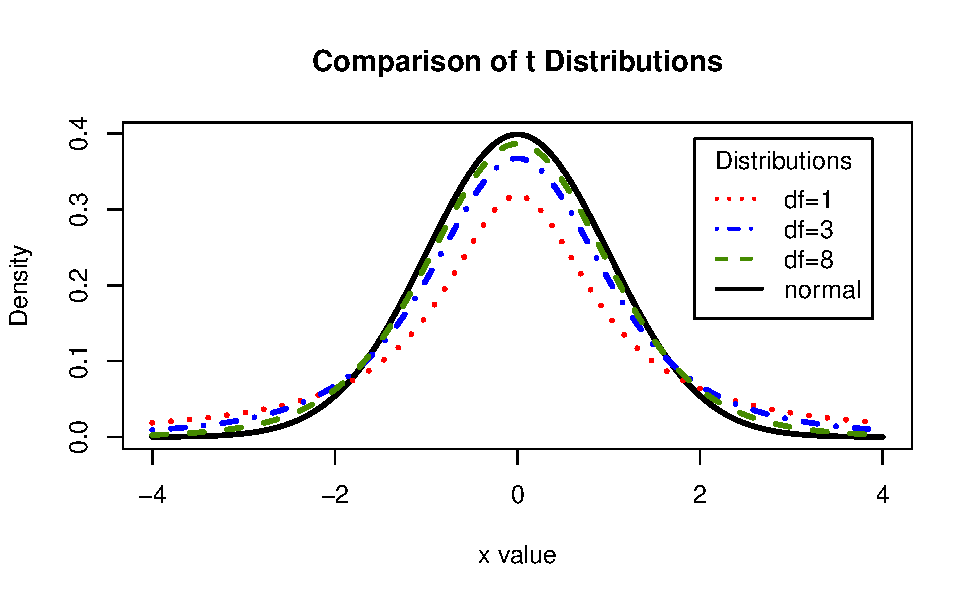
\includegraphics[width=0.7\linewidth]{06-A13-quantitative_theory_files/figure-latex/tdist-1} 

}

\caption{Comparison of the standard Normal vs t-distribution with various degrees of freedom}\label{fig:tdist}
\end{figure}

\subsubsection*{Summarize and visualize the data}\label{summarize-and-visualize-the-data-2}
\addcontentsline{toc}{subsubsection}{Summarize and visualize the data}

The following code is used to create a boxplot of the data.

\begin{itemize}
\item
  Download the R script file upload to the R studio server.
\item
  Open the R script file and highlight and run lines 1--14.
\end{itemize}

\begin{Shaded}
\begin{Highlighting}[]
\NormalTok{bodytemp }\OtherTok{\textless{}{-}} \FunctionTok{read.csv}\NormalTok{(}\StringTok{"https://math.montana.edu/courses/s216/data/normal\_temperature.csv"}\NormalTok{)}
\NormalTok{bodytemp }\SpecialCharTok{\%\textgreater{}\%}
  \FunctionTok{ggplot}\NormalTok{(}\FunctionTok{aes}\NormalTok{(}\AttributeTok{x =}\NormalTok{ Temp))}\SpecialCharTok{+}
  \FunctionTok{geom\_boxplot}\NormalTok{()}\SpecialCharTok{+}
  \FunctionTok{labs}\NormalTok{(}\AttributeTok{title=}\StringTok{"Boxplot of Body Temperatures for Stat 216 Students"}\NormalTok{,}
       \AttributeTok{x =} \StringTok{"body temperature (*F)"}\NormalTok{) }\SpecialCharTok{+}
        \FunctionTok{theme}\NormalTok{(}\AttributeTok{axis.text.y =} \FunctionTok{element\_blank}\NormalTok{(), }
          \AttributeTok{axis.ticks.y =} \FunctionTok{element\_blank}\NormalTok{()) }\CommentTok{\# Removes y{-}axis ticks}
\end{Highlighting}
\end{Shaded}

\begin{center}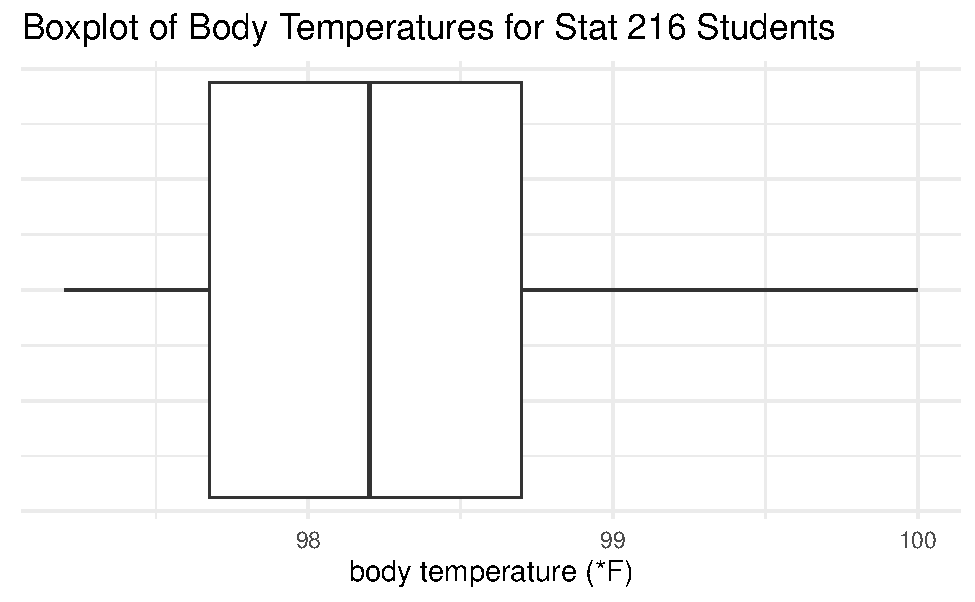
\includegraphics[width=0.7\linewidth]{06-A13-quantitative_theory_files/figure-latex/unnamed-chunk-1-1} \end{center}

\begin{itemize}
\tightlist
\item
  Highlight and run lines 17 - 18 to get the summary statistics for the variable \texttt{Temp}.
\end{itemize}

\begin{Shaded}
\begin{Highlighting}[]
\NormalTok{bodytemp }\SpecialCharTok{\%\textgreater{}\%} 
  \FunctionTok{summarise}\NormalTok{(}\FunctionTok{favstats}\NormalTok{(Temp))}
\end{Highlighting}
\end{Shaded}

\begin{verbatim}
#>    min     Q1 median   Q3 max     mean        sd  n missing
#> 1 97.2 97.675   98.2 98.7 100 98.28462 0.6823789 52       0
\end{verbatim}

\subsubsection*{Check theoretical conditions}\label{check-theoretical-conditions}
\addcontentsline{toc}{subsubsection}{Check theoretical conditions}

\begin{enumerate}
\def\labelenumi{\arabic{enumi}.}
\setcounter{enumi}{2}
\tightlist
\item
  Report the sample size of the study. Give appropriate notation.
\end{enumerate}

\vspace{0.3in}

\begin{enumerate}
\def\labelenumi{\arabic{enumi}.}
\setcounter{enumi}{3}
\tightlist
\item
  Report the sample mean of the study. Give appropriate notation.
\end{enumerate}

\vspace{0.3in}

\begin{enumerate}
\def\labelenumi{\arabic{enumi}.}
\setcounter{enumi}{4}
\item
  How do you know the independence condition is met for these data?
  \vspace{0.8in}
\item
  Is the normality condition met to use the theory-based methods for analysis? Explain your answer.
  \vspace{1in}
\end{enumerate}

\newpage

\subsubsection*{Use statistical inferential methods to draw inferences from the data}\label{use-statistical-inferential-methods-to-draw-inferences-from-the-data}
\addcontentsline{toc}{subsubsection}{Use statistical inferential methods to draw inferences from the data}

To find the standardized statistic for the mean we will use the following formula:

\[T = \frac{\bar{x} - \mu_0}{SE(\bar{x})},\]
where the standard error of the sample mean is:

\[SE(\bar{x})=\frac{s}{\sqrt{n}}.\]

\begin{enumerate}
\def\labelenumi{\arabic{enumi}.}
\setcounter{enumi}{6}
\tightlist
\item
  Calculate the standard error of the sample mean.
\end{enumerate}

\vspace{0.5in}

\begin{enumerate}
\def\labelenumi{\arabic{enumi}.}
\setcounter{enumi}{7}
\tightlist
\item
  Interpret the standard error in context of the study.
\end{enumerate}

\vspace{1in}

\begin{enumerate}
\def\labelenumi{\arabic{enumi}.}
\setcounter{enumi}{8}
\tightlist
\item
  Calculate the standardized mean.
\end{enumerate}

\vspace{1in}

\begin{enumerate}
\def\labelenumi{\arabic{enumi}.}
\setcounter{enumi}{9}
\tightlist
\item
  We model a single mean with a \(t\)-distribution with \(n-1\) degrees of freedom. Calculate the degrees of freedom for this study and use it to fill in the blank in the title of the \(t\)-distribution displayed below.
\end{enumerate}

\vspace{0.2in}

\begin{enumerate}
\def\labelenumi{\arabic{enumi}.}
\setcounter{enumi}{10}
\tightlist
\item
  Mark the value of the standardized statistic on the \(t\)-distribution and illustrate how the p-value is found.
\end{enumerate}

\begin{center}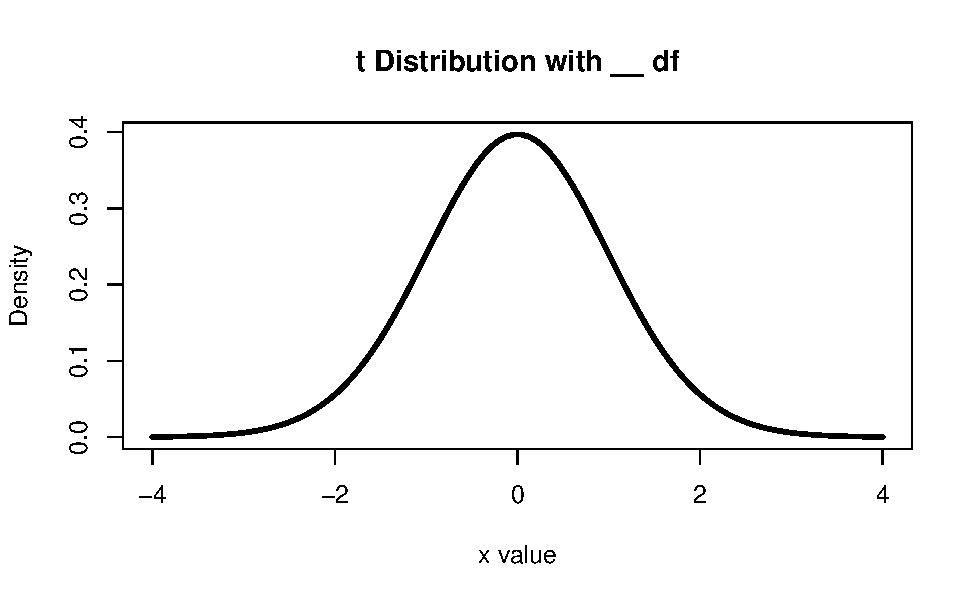
\includegraphics[width=0.7\linewidth]{06-A13-quantitative_theory_files/figure-latex/tdistmean-1} \end{center}
\newpage

To find the p-value for the theory-based test in R:

\begin{itemize}
\item
  Enter the value for the standardized statistic for \texttt{xx} in the \texttt{pt} function.
\item
  Enter the degrees of freedom for \texttt{yy} in the \texttt{pt} function.
\item
  Highlight and run line 24.
\end{itemize}

\begin{Shaded}
\begin{Highlighting}[]
\FunctionTok{pt}\NormalTok{(xx, }\AttributeTok{df=}\NormalTok{yy, }\AttributeTok{lower.tail=}\ConstantTok{FALSE}\NormalTok{)}
\end{Highlighting}
\end{Shaded}

\begin{enumerate}
\def\labelenumi{\arabic{enumi}.}
\setcounter{enumi}{11}
\item
  What does this p-value mean, in the context of the study? Hint: it is the probability of what\ldots assuming what?
  \vspace{1in}
\item
  Write a conclusion to the test in context of the study.
\end{enumerate}

\vspace{0.6in}

\begin{enumerate}
\def\labelenumi{\arabic{enumi}.}
\setcounter{enumi}{13}
\tightlist
\item
  Can we generalize the results of the study to all adults? Explain your answer.
\end{enumerate}

\vspace{0.5in}

\subsection{Take-home messages}\label{take-home-messages-12}

\begin{enumerate}
\def\labelenumi{\arabic{enumi}.}
\item
  In order to use theory-based methods for a quantitative variable, the independent observational units and normality conditions must be met.
\item
  In order to find a theory-based p-value, we use R to calculate the area under a \(t\)-distribution with \(n - 1\) degrees of freedom (df) that is at or more extreme than the observed \(T\)-score. To find a two-sided p-value using theory-based methods we need to multiply the one-sided p-value by 2.
\item
  A \(t^*\) multiplier is found by obtaining the bounds of the middle X\% (X being the desired confidence level) of a \(t\)-distribution with \(n - 1\) df.
\end{enumerate}

\subsection{Additional notes}\label{additional-notes-12}

Use this space to summarize your thoughts and take additional notes on today's activity and material covered

\newpage

\chapter{Confidence Intervals for a Single Quantitative Variable}\label{confidence-intervals-for-a-single-quantitative-variable}

\section{Vocabulary Review and Key Topics}\label{vocabulary-review-and-key-topics-5}

Review the Golden Ticket posted in the resources at the end of the coursepack for a summary of a single quantitative variable.

\subsection{Key topics}\label{key-topics-6}

Module 7 will cover creating confidence intervals using both simulation-based and theory-based methods. Additionally, we learn about types of errors and power in hypothesis testing.

\subsubsection*{Simulation-based confidence interval}\label{simulation-based-confidence-interval}
\addcontentsline{toc}{subsubsection}{Simulation-based confidence interval}

\begin{itemize}
\item
  Review the conditions necessary for simulation-based inference in Module 6.
\item
  R code to find the simulation-based confidence interval using the \texttt{onemean\_CI} function from the \texttt{catstats} package.

\begin{Shaded}
\begin{Highlighting}[]
\FunctionTok{one\_mean\_CI}\NormalTok{(object}\SpecialCharTok{$}\NormalTok{variable, }\CommentTok{\#Enter the name of the variable}
        \AttributeTok{summary\_measure =} \StringTok{"mean"}\NormalTok{, }\CommentTok{\#choose the mean or median}
        \AttributeTok{number\_repetitions =} \DecValTok{10000}\NormalTok{,  }\CommentTok{\# Number of simulations}
        \AttributeTok{confidence\_level =}\NormalTok{ xx)}
\end{Highlighting}
\end{Shaded}
\item
  Interpretation of the confidence interval is very similar as for a single proportion only the context and summary measure has changed.

  \begin{itemize}
  \item
    To write in context include:

    \begin{itemize}
    \item
      How confident you are (e.g., 90\%, 95\%, 98\%, 99\%)
    \item
      Parameter of interest
    \item
      Calculated interval
    \end{itemize}
  \end{itemize}
\end{itemize}

\subsubsection*{Theory-based confidence interval}\label{theory-based-confidence-interval-1}
\addcontentsline{toc}{subsubsection}{Theory-based confidence interval}

\begin{itemize}
\item
  Review the conditions necessary for theory-based inference in Module 6.
\item
  \textbf{Margin of error}: half the width of the confidence interval. For a single mean, the margin of error is:
  \[ME = t^* \times SE(\bar{x})\]
  where \(t^*\) is the \textbf{multiplier}, corresponding to the desired confidence level found from a \(t\)-distribution with \(n-1\) degrees of freedom and \[SE(\bar{x}) = \frac{s}{\sqrt{n}}.\]
\item
  To find the endpoints of a confidence interval, add and subtract the margin of error to the sample statistic. The confidence interval for a population mean is:
  \[\bar{x} \pm ME\]
\end{itemize}

\newpage

\begin{itemize}
\item
  R code to find the \textbf{multiplier} for a confidence interval using theory-based methods involving means.

  \begin{itemize}
  \item
    \texttt{qt} will give you the multiplier using a \(t\)-distribution with a given degrees of freedom (enter for \texttt{yy}). For a single mean, \texttt{df} = \(n - 1\).
  \item
    Enter the percentile for the given level of confidence (e.g., 0.975 for a 95\% confidence level).
  \end{itemize}

\begin{Shaded}
\begin{Highlighting}[]
\FunctionTok{qt}\NormalTok{(percentile, }\AttributeTok{df =}\NormalTok{ yy, }\AttributeTok{lower.tail=}\ConstantTok{FALSE}\NormalTok{)}
\end{Highlighting}
\end{Shaded}
\end{itemize}

\subsection*{Vocabulary}\label{vocabulary-5}
\addcontentsline{toc}{subsection}{Vocabulary}

\begin{itemize}
\item
  \textbf{Significance level (\(\alpha\))}: a given cut-off value that we compare the p-value to determine a decision of a test.
\item
  \textbf{Decisions}:

  \begin{itemize}
  \item
    If the p-value is less than the significance level, we make the decision to \emph{reject the null hypothesis}.
  \item
    If the p-value is greater than the significance level, we make the decision to \emph{fail to reject the null hypothesis}.
  \end{itemize}
\item
  \textbf{Type 1 Error}: concluding there is evidence to reject the null hypothesis, when the null is actually true.

  \begin{itemize}
  \tightlist
  \item
    The probability of making a Type 1 error when the null is actually true is equal to the significance level, \(\alpha\).
  \end{itemize}
\item
  \textbf{Type 2 Error}: concluding there is no evidence to reject the null hypothesis, when the null is actually false.
\item
  \textbf{Power}: probability of concluding there is evidence to reject the null hypothesis, when the null is actually false.

  \begin{itemize}
  \tightlist
  \item
    When the null is actually false, the event ``reject the null hypothesis'' is the \emph{complement} of the event ``fail to reject the null hypothesis.'' Thus, power is equal to 1 minus the probability of a Type 2 error.
  \end{itemize}
\end{itemize}

\newpage

\section{Video Notes: Theory-based Inference for a single quantitative variable}\label{video-notes-theory-based-inference-for-a-single-quantitative-variable}

Read Chapters 5 and 17 in the course textbook. Use the following videos to complete the video notes for Module 7.

\subsection{Course Videos}\label{course-videos-5}

\begin{itemize}
\item
  17.1
\item
  17.3TheoryIntervals
\end{itemize}

\setstretch{1}

\subsection{Single quantitative variable}\label{single-quantitative-variable}

\begin{itemize}
\item
  Reminder: review summary measures and plots discussed in the Module 6 material and Chapter 5 of the textbook.
\item
  The summary measure for a single quantitative variable is the \_\_\_\_\_\_\_\_\_\_\_\_\_\_.
\end{itemize}

\setstretch{1.5}

Notation:

\begin{itemize}
\item
  Population mean:
\item
  Population standard deviation:
\item
  Sample mean:
\item
  Sample standard deviation:
\item
  Sample size:
\end{itemize}

\setstretch{1}

Example: What is the average weight of adult male polar bears? The weight was measured on a representative sample of 83 male polar bears from the Southern Beaufort Sea.

\begin{Shaded}
\begin{Highlighting}[]
\NormalTok{pb }\OtherTok{\textless{}{-}} \FunctionTok{read.csv}\NormalTok{(}\StringTok{"https://math.montana.edu/courses/s216/data/polarbear.csv"}\NormalTok{)}
\end{Highlighting}
\end{Shaded}

Plots of the data:

\begin{Shaded}
\begin{Highlighting}[]
\NormalTok{pb }\SpecialCharTok{\%\textgreater{}\%}
    \FunctionTok{ggplot}\NormalTok{(}\FunctionTok{aes}\NormalTok{(}\AttributeTok{x =}\NormalTok{ Weight)) }\SpecialCharTok{+}   \CommentTok{\# Name variable to plot}
    \FunctionTok{geom\_histogram}\NormalTok{(}\AttributeTok{binwidth =} \DecValTok{10}\NormalTok{) }\SpecialCharTok{+}  \CommentTok{\# Create histogram with specified binwidth}
    \FunctionTok{labs}\NormalTok{(}\AttributeTok{title =} \StringTok{"Histogram of Male Polar Bear Weight"}\NormalTok{, }\CommentTok{\# Title for plot}
       \AttributeTok{x =} \StringTok{"Weight (kg)"}\NormalTok{, }\CommentTok{\# Label for x axis}
       \AttributeTok{y =} \StringTok{"Frequency"}\NormalTok{) }\CommentTok{\# Label for y axis}

\NormalTok{pb }\SpecialCharTok{\%\textgreater{}\%} \CommentTok{\# Data set piped into...}
\FunctionTok{ggplot}\NormalTok{(}\FunctionTok{aes}\NormalTok{(}\AttributeTok{x =}\NormalTok{ Weight)) }\SpecialCharTok{+}   \CommentTok{\# Name variable to plot}
  \FunctionTok{geom\_boxplot}\NormalTok{() }\SpecialCharTok{+}  \CommentTok{\# Create boxplot}
  \FunctionTok{labs}\NormalTok{(}\AttributeTok{title =} \StringTok{"Boxplot of Male Polar Bear Weight"}\NormalTok{, }\CommentTok{\# Title for plot}
       \AttributeTok{x =} \StringTok{"Weight (kg)"}\NormalTok{, }\CommentTok{\# Label for x axis}
       \AttributeTok{y =} \StringTok{"Frequency"}\NormalTok{) }\CommentTok{\# Label for y axis}
\end{Highlighting}
\end{Shaded}

\begin{center}\includegraphics[width=0.6\linewidth]{07-VN07-one_meantheory_files/figure-latex/unnamed-chunk-2-1} \includegraphics[width=0.6\linewidth]{07-VN07-one_meantheory_files/figure-latex/unnamed-chunk-2-2} \end{center}

Summary Statistics:

\begin{Shaded}
\begin{Highlighting}[]
\NormalTok{pb }\SpecialCharTok{\%\textgreater{}\%}
  \FunctionTok{summarise}\NormalTok{(}\FunctionTok{favstats}\NormalTok{(Weight)) }\CommentTok{\#Gives the summary statistics}
\CommentTok{\#\textgreater{}     min    Q1 median     Q3   max     mean       sd  n missing}
\CommentTok{\#\textgreater{} 1 104.1 276.3  339.4 382.45 543.6 324.5988 88.32615 83       0}
\end{Highlighting}
\end{Shaded}

\subsection*{Confidence interval}\label{confidence-interval}
\addcontentsline{toc}{subsection}{Confidence interval}

\subsubsection*{Simulation-based method}\label{simulation-based-method-3}
\addcontentsline{toc}{subsubsection}{Simulation-based method}

\begin{itemize}
\item
  Label cards with the values from the data set
\item
  Sample with replacement (bootstrap) from the original sample \(n\) times
\item
  Plot the simulated sample mean on the bootstrap distribution
\item
  Repeat at least 10000 times (simulations)
\item
  Find the cut-offs for the middle X\% (confidence level) in a bootstrap distribution.
\item
  ie. 95\% CI = (2.5th percentile, 97.5th percentile)
\end{itemize}

Conditions for inference for a single mean:

\begin{itemize}
\tightlist
\item
  Independence:
\end{itemize}

\vspace{0.5in}

\begin{Shaded}
\begin{Highlighting}[]
\FunctionTok{set.seed}\NormalTok{(}\DecValTok{216}\NormalTok{)}
\FunctionTok{one\_mean\_CI}\NormalTok{(pb}\SpecialCharTok{$}\NormalTok{Weight,}
  \AttributeTok{summary\_measure =} \StringTok{"mean"}\NormalTok{,}
  \AttributeTok{number\_repetitions =} \DecValTok{10000}\NormalTok{,}
  \AttributeTok{confidence\_level =} \FloatTok{0.95}\NormalTok{)}
\end{Highlighting}
\end{Shaded}

\begin{center}\includegraphics[width=0.7\linewidth]{07-VN07-one_meantheory_files/figure-latex/unnamed-chunk-4-1} \end{center}

The confidence interval estimates the \_\_\_\_\_\_\_\_\_\_\_\_\_\_\_\_
of \_\_\_\_\_\_\_\_\_\_\_\_\_\_\_\_\_\_\_\_.

Confidence interval interpretation:

\begin{itemize}
\item
  How confident you are (e.g., 90\%, 95\%, 98\%, 99\%)
\item
  Parameter of interest
\item
  Calculated interval
\item
  Order of subtraction when comparing two groups
\end{itemize}

\vspace{0.8in}

\newpage

\subsubsection*{Theory-based method}\label{theory-based-method-2}
\addcontentsline{toc}{subsubsection}{Theory-based method}

\begin{itemize}
\tightlist
\item
  Calculate the interval centered at the sample statistic
\end{itemize}

\rgi \(\text{statistic} \pm \text{margin of error}\)

\vspace{0.5in}

Conditions for inference using theory-based methods:

\begin{itemize}
\tightlist
\item
  Independence:
\end{itemize}

\vspace{0.2in}

\begin{itemize}
\tightlist
\item
  Large enough sample size:
\end{itemize}

\vspace{0.2in}

\subsection*{\texorpdfstring{\(t\)-distribution}{t-distribution}}\label{t-distribution-1}
\addcontentsline{toc}{subsection}{\(t\)-distribution}

In the theoretical approach, we use the CLT to tell us that the distribution of sample means will be approximately normal, centered at the assumed true mean under \(H_0\) and with standard deviation \(\frac{\sigma}{\sqrt{n}}\).

\[\bar{x} \sim N\left(\mu_0, \frac{\sigma}{\sqrt{n}}\right)\]
\setstretch{1.5}

\begin{itemize}
\item
  Estimate the population standard deviation, \(\sigma\), with the
  \_\_\_\_\_\_\_\_\_\_\_\_\_\_\_\_\_\_\_\_\_\_\_\_\_\_\_ standard deviation, \_\_\_\_\_\_\_\_.
\item
  For a single quantitative variable we use the \_\_\_\_ - distribution
  with \_\_\_\_\_\_\_\_\_\_\_\_\_\_\_
  degrees of freedom to approximate the sampling distribution.
\end{itemize}

\setstretch{1}

The \(t^*\) multiplier is the value at the given percentile of the t-distribution with \(n - 1\) degrees of freedom.

\begin{center}\includegraphics[width=0.7\linewidth]{07-VN07-one_meantheory_files/figure-latex/tstarpb-1} \end{center}

\newpage

To find the \(t^*\) multiplier for a 95\% confidence interval:

\begin{Shaded}
\begin{Highlighting}[]
\FunctionTok{qt}\NormalTok{(}\FloatTok{0.975}\NormalTok{, }\AttributeTok{df =} \DecValTok{82}\NormalTok{)}
\CommentTok{\#\textgreater{} [1] 1.989319}
\end{Highlighting}
\end{Shaded}

Calculation of the confidence interval for the true mean weight of polar bears from the Southern Beaufort Sea:

\vspace{0.8in}

\subsection{Concept Check}\label{concept-check-6}

Be prepared for group discussion in the next class. One member from the table should write the answers to the following on the whiteboard.

\begin{enumerate}
\def\labelenumi{\arabic{enumi}.}
\tightlist
\item
  Are the conditions met to analyze the polar bear data using theory-based methods?
\end{enumerate}

\vspace{0.7in}

\begin{enumerate}
\def\labelenumi{\arabic{enumi}.}
\setcounter{enumi}{1}
\tightlist
\item
  Interpret the confidence interval found with simulation methods.
\end{enumerate}

\vspace{0.2in}

\newpage

\section{Activity 14: Danceability of Songs}\label{activity-14-danceability-of-songs}

\setstretch{1}

\subsection{Learning outcomes}\label{learning-outcomes-14}

\begin{itemize}
\item
  Use simulation-based methods to find a confidence interval for a single mean.
\item
  Use theory-based methods to find a confidence interval for a single mean.
\item
  Interpret a confidence interval for a single mean.
\item
  Use a confidence interval to determine the conclusion of a hypothesis test.
\end{itemize}

\subsection{Terminology review}\label{terminology-review-12}

In today's activity, we will estimate the parameter of interest using simulation-based and theory-based methods. Some terms covered in this activity are:

\begin{itemize}
\item
  Bootstrap distribution
\item
  \(t\)-distribution
\item
  Degrees of freedom
\item
  \(T\)-score
\end{itemize}

To review these concepts, see Chapter 17 in the textbook.

\subsection{Danceability}\label{danceability}

Spotify created a list of the top songs around the world for the past 10 years and several different audio features of those songs. One of the variables measured on these songs is ``danceability.'' Danceability measures how easy it is to dance to a song; the higher the point value the easier it is to dance to the song. Estimate the average danceability of top songs from Spotify.

\begin{itemize}
\item
  Download the R script file for this activity from D2L and upload to the RStudio server.
\item
  Open the R script file, highlight and run the lines to load libraries and the code below.
\end{itemize}

\begin{verbatim}
#>   min Q1 median Q3 max     mean       sd   n missing
#> 1   0 57     66 73  97 64.37977 13.37872 603       0
\end{verbatim}

\begin{Shaded}
\begin{Highlighting}[]
\NormalTok{songs }\SpecialCharTok{\%\textgreater{}\%} \CommentTok{\# Data set piped into...}
    \FunctionTok{ggplot}\NormalTok{(}\FunctionTok{aes}\NormalTok{(}\AttributeTok{x =}\NormalTok{ Danceability)) }\SpecialCharTok{+}   \CommentTok{\# Name variable to plot}
    \FunctionTok{geom\_boxplot}\NormalTok{() }\SpecialCharTok{+}  \CommentTok{\# Create boxplot with specified binwidth}
    \FunctionTok{labs}\NormalTok{(}\AttributeTok{title =} \StringTok{"Boxplot of Danceability Score for Top Spotify Songs"}\NormalTok{, }\CommentTok{\# Title for plot}
         \AttributeTok{x =} \StringTok{"danceability score (points)"}\NormalTok{, }\CommentTok{\# Label for x axis}
         \AttributeTok{y =} \StringTok{""}\NormalTok{) }\SpecialCharTok{+} \CommentTok{\# Remove y axis label}
    \FunctionTok{theme}\NormalTok{(}\AttributeTok{axis.text.y =} \FunctionTok{element\_blank}\NormalTok{(), }
          \AttributeTok{axis.ticks.y =} \FunctionTok{element\_blank}\NormalTok{()) }\CommentTok{\# Removes y{-}axis ticks}
\end{Highlighting}
\end{Shaded}

\begin{center}\includegraphics[width=0.7\linewidth]{07-A14-onemean-CI_files/figure-latex/unnamed-chunk-2-1} \end{center}

\subsubsection*{Summarizing quantitative variables}\label{summarizing-quantitative-variables-2}
\addcontentsline{toc}{subsubsection}{Summarizing quantitative variables}

\begin{enumerate}
\def\labelenumi{\arabic{enumi}.}
\tightlist
\item
  Describe the distribution of danceability of top songs over the past 10 years on Spotify.
\end{enumerate}

\vspace{0.8in}

\begin{enumerate}
\def\labelenumi{\arabic{enumi}.}
\setcounter{enumi}{1}
\tightlist
\item
  Write the parameter of interest in context of the study.
\end{enumerate}

\vspace{0.8in}

\subsection*{Simulation methods to create a confidence interval}\label{simulation-methods-to-create-a-confidence-interval}
\addcontentsline{toc}{subsection}{Simulation methods to create a confidence interval}

Unlike creation of the null distribution, the bootstrap distribution we use for creating a confidence interval is found by sampling with replacement from the original sample. To create one dot on the bootstrap distribution:

\begin{itemize}
\item
  Write the original values for the variable on \(n\) cards; one card for each observational unit.
\item
  Sample with replacement from the cards \(n\) times.
\item
  Plot the mean from each resampled sample on the bootstrap distribution.
\end{itemize}

Use the provided R script file to find a 95\% confidence interval.

\begin{itemize}
\item
  Enter the name of the variable for \texttt{variable}.
\item
  Enter the appropriate confidence level for \texttt{xx}.
\item
  Highlight and run lines 22--25.
\end{itemize}

\begin{Shaded}
\begin{Highlighting}[]
\FunctionTok{one\_mean\_CI}\NormalTok{(songs}\SpecialCharTok{$}\NormalTok{variable, }\CommentTok{\#Enter the name of the variable}
            \AttributeTok{summary\_measure =} \StringTok{"mean"}\NormalTok{, }\CommentTok{\#choose the mean or median}
            \AttributeTok{number\_repetitions =} \DecValTok{10000}\NormalTok{,  }\CommentTok{\# Number of simulations}
            \AttributeTok{confidence\_level =}\NormalTok{ xx)}
\end{Highlighting}
\end{Shaded}

\begin{enumerate}
\def\labelenumi{\arabic{enumi}.}
\setcounter{enumi}{2}
\tightlist
\item
  Report the 95\% confidence interval for the parameter of interest.
\end{enumerate}

\vspace{0.2in}

\subsection*{Theory-based methods to create a confidence interval}\label{theory-based-methods-to-create-a-confidence-interval}
\addcontentsline{toc}{subsection}{Theory-based methods to create a confidence interval}

\begin{itemize}
\item
  \textbf{Conditions for the sampling distribution of \(\bar{x}\) to follow an approximate normal distribution}:

  \begin{itemize}
  \item
    \textbf{Independence}: The sample's observations are independent, e.g., are from a simple random sample. (\emph{Remember}: This also must be true to use simulation methods!)
  \item
    \textbf{Normality Condition}: Either the sample observations come from a normally distributed population or we have a large enough sample size. To check this condition, use the following rules of thumb:

    \begin{itemize}
    \item
      \(n < 30\): The distribution of the sample must be approximately normal with no outliers.
    \item
      \(30 \le n < 100\): We can relax the condition a little; the distribution of the sample must have no extreme outliers or skewness.
    \item
      \(n \ge 100\): Can assume the sampling distribution of \(\bar{x}\) is nearly normal, even if the underlying distribution of individual observations is not.
    \end{itemize}
  \end{itemize}
\end{itemize}

Next we will calculate a theory-based confidence interval. To calculate a theory-based confidence interval for the a single mean, use the following formula:

\[\bar{x}\pm t^* \times SE(\bar{x}).\]

We will need to find the \(t^*\) multiplier using the function \texttt{qt()}.

\begin{itemize}
\item
  Enter the appropriate percentile in the R code to find the multiplier for a 95\% confidence interval.
\item
  Enter the degrees of freedom for \texttt{yy}. \emph{The degrees of freedom for a single mean is \(n-1\)}.
\item
  Highlight and run line 31.
\end{itemize}

\begin{Shaded}
\begin{Highlighting}[]
\FunctionTok{qt}\NormalTok{(percentile, }\AttributeTok{df =}\NormalTok{ yy, }\AttributeTok{lower.tail=}\ConstantTok{TRUE}\NormalTok{)}
\end{Highlighting}
\end{Shaded}

\begin{enumerate}
\def\labelenumi{\arabic{enumi}.}
\setcounter{enumi}{3}
\tightlist
\item
  Mark on the \(t\)-distribution found below the values of \(\pm t^*\). Draw a line at each multiplier and write the percentiles used to find each.
  \vspace{1mm}
\end{enumerate}

\begin{figure}

{\centering \includegraphics[width=0.75\linewidth]{07-A14-onemean-CI_files/figure-latex/tst-1} 

}

\end{figure}

\newpage

\begin{enumerate}
\def\labelenumi{\arabic{enumi}.}
\setcounter{enumi}{4}
\tightlist
\item
  Calculate the margin of error using theory-based methods.
\end{enumerate}

\vspace{0.6in}

\begin{enumerate}
\def\labelenumi{\arabic{enumi}.}
\setcounter{enumi}{5}
\tightlist
\item
  Calculate the confidence interval for the true mean using theory-based methods.
\end{enumerate}

\vspace{0.6in}

\begin{enumerate}
\def\labelenumi{\arabic{enumi}.}
\setcounter{enumi}{6}
\tightlist
\item
  Interpret the confidence interval in context of the study.
\end{enumerate}

\vspace{1in}

\begin{enumerate}
\def\labelenumi{\arabic{enumi}.}
\setcounter{enumi}{7}
\tightlist
\item
  Explain why the confidence interval with theory-based methods is similar to the confidence interval found using the bootstrap distribution.
\end{enumerate}

\vspace{1in}

\subsection{Take-home messages}\label{take-home-messages-13}

\begin{enumerate}
\def\labelenumi{\arabic{enumi}.}
\item
  In order to use theory-based methods for a single mean, the independent observational units and normality conditions must be met.
\item
  The simulation-based confidence interval and theory-based confidence interval should be similar if the normality condition is met.
\item
  A \(t^*\) multiplier is found by obtaining the bounds of the middle X\% (X being the desired confidence level) of a \(t\)-distribution with \(n - 1\) df.
\end{enumerate}

\subsection{Additional notes}\label{additional-notes-13}

Use this space to summarize your thoughts and take additional notes on today's activity and material covered

\newpage

\section{Activity 15: Errors and Power}\label{activity-15-errors-and-power}

\setstretch{1}

\subsection{Learning outcomes}\label{learning-outcomes-15}

\begin{itemize}
\item
  Explain Type I and Type 2 errors in the context of a study.
\item
  Explain the power of a test in the context of a study.
\item
  Understand how changes in sample size, significance level, and the difference between the null value and the parameter value impact the power of a test.
\item
  Understand how significance level impacts the probability of a Type 1 error.
\item
  Understand the relationship between the probability of a Type 2 error and power.
\item
  Be able to distinguish between practical importance and statistical significance.
\end{itemize}

\subsection{Terminology review}\label{terminology-review-13}

In this activity, we will examine the possible errors that can be made based on the decision in a hypothesis test as well as factors influencing the power of the test. Some terms covered in this activity are:

\begin{itemize}
\item
  Significance level
\item
  Type 1 error
\item
  Type 2 error
\item
  Power
\end{itemize}

To review these concepts, see Chapter 12 in the textbook.

\subsection{College textbook cost}\label{college-textbook-cost}

A college student spends, on average, \$280 on textbooks per year. Many universities have started using open-source resources to help defray the cost of textbooks. One such university is hoping to show they have successfully reduced costs by \$100 per year, on average.

\begin{enumerate}
\def\labelenumi{\arabic{enumi}.}
\item
  Write the parameter of interest (\(\mu\)) in words, in the context of this problem.
  \vspace{0.5in}
\item
  Use proper notation to write the null and alternative hypotheses the university would need to test in order to check their claim.
  \vspace{0.5in}
\end{enumerate}

After determining hypotheses and prior to collecting data, researchers should set a \textbf{significance level} for a hypothesis test. The significance level, represented by \(\alpha\) and most commonly 0.01, 0.05, or 0.10, is a cut-off for determining whether a p-value is small or not. The \emph{smaller} the p-value, the \emph{stronger} the evidence against the null hypothesis, so a p-value that is smaller than or equal to the significance level is strong enough evidence to \emph{reject the null hypothesis}. Similarly, the \emph{larger} the p-value, the \emph{weaker} the evidence against the null hypothesis, so a p-value that is larger than the significance level does not provide enough evidence against the null hypothesis and the researcher would \emph{fail to reject the null hypothesis}. Rejecting the null hypothesis or failing to reject the null hypothesis are the two \textbf{decisions} that can be made based on the data collected.

As you have already learned in this course, sample size of a study is extremely important. Often times, researchers will conduct what is called a power analysis to determine the appropriate sample size based on the goals of their research, including a desired \textbf{power} of their test. Power is the probability of correctly rejecting the null hypothesis, or the probability of the data providing strong evidence against the null hypothesis \emph{when the null hypothesis is false}.

The remainder of this activity will be spent investigating how different factors influence the power of a test, after which you will complete a power analysis for this university.

\begin{itemize}
\item
  Navigate to \url{https://istats.shinyapps.io/power/}.
\item
  Choose the tab ``Population Mean''.
\item
  Use the scale under ``Null Hypothesis value \(\mu_0\)'' to change the value to your null value from question 2. *Note we will convert this to a scale in hundreds of dollars (e.g., 1 = \$100). In other words, use the null value of 2.8.
\item
  Change the ``Alternative Hypothesis'' to the direction you wrote in question 2.
\item
  Leave all boxes un-checked.
\item
  Set the ``True value of \(\mu\)'' to 2.8 as well.
\item
  Do not change the scales for ``Sample size n'' or ``Type I Error \(\alpha\)'' or ``Population Std. Dev. \(\sigma\)''.
\end{itemize}

The red distribution you see is the scaled-Normal distribution representing the null distribution for this hypothesis test, if the sample size was \(n = 30\) and the significance level was \(\alpha = 0.05\). This means the red distribution is showing the distribution of possible sample mean amounts spent on textbooks per year (in hundreds of dollars) for a sample of 30 college students (\(\bar{x}\)) if we assume the null hypothesis is true.

\begin{enumerate}
\def\labelenumi{\arabic{enumi}.}
\setcounter{enumi}{2}
\item
  Based off this distribution and your alternative hypothesis, give one possible sample mean which you think would lead to rejecting the null hypothesis. Explain how you decided on your value.
  \vspace{0.25in}
\item
  Check the box for ``Show Critical Value(s) and Rejection Region(s)''. You will now see a vertical line on the plot indicating the \emph{maximum} sample mean which would lead to reject the null hypothesis. That is, any sample means below this value would lead us to reject the null hypothesis; any sample means below this value would lead us to fail to reject the null hypothesis. What is this value?\\
  \vspace{0.25in}
\item
  Notice that there are some sample means under the red line (when the null hypothesis is true) which would lead us to reject the null hypothesis. Give the range of sample means which would lead to rejecting the null hypothesis when the null hypothesis is true? What is the statistical name for this mistake?
  \vspace{0.4in}
\end{enumerate}

Check the ``Type I Error'' box under \textbf{Display}. This should verify (or correct) your answer to question 5! The area shaded in red represents the probability of making a \textbf{Type 1 Error} in our hypothesis test. Recall that a Type 1 error is when we reject the null hypothesis even though the null hypothesis is true. To reject the null hypothesis, the p-value, which was found assuming the null hypothesis is true, must be less than or equal to the significance level. Therefore the significance level is the probability of rejecting the null hypothesis when the null hypothesis is true, so the significance level IS the probability of making a Type 1 error in a hypothesis test!

\begin{enumerate}
\def\labelenumi{\arabic{enumi}.}
\setcounter{enumi}{5}
\tightlist
\item
  Based on the current applet settings, what percent of the null distribution is shaded red (i.e., what is the probability of making a Type 1 error)?
  \vspace{0.25in}
\end{enumerate}

\newpage

Let's say this university believes their program can reduce the cost of textbooks for college students by \$100 per year. In the applet, set the scale under ``True value of \(\mu\)'' to 1.8.

\begin{enumerate}
\def\labelenumi{\arabic{enumi}.}
\setcounter{enumi}{6}
\tightlist
\item
  Where is the blue distribution centered?
  \vspace{0.25in}
\end{enumerate}

The blue distribution that appears represents what the university believes, that \$180 (not \$280) is the true mean textbook cost for college students at this university. This blue distribution represents the idea that the \textbf{null hypothesis is false}.

\begin{enumerate}
\def\labelenumi{\arabic{enumi}.}
\setcounter{enumi}{7}
\tightlist
\item
  Consider the definition of power provided earlier in this activity. Do you believe the power of the test will be an area within the blue distribution or red distribution? How do you know? What about the probability of making a Type 2 error?
  \vspace{1in}
\end{enumerate}

Check the ``Type II Error'' and ``Power'' boxes under \textbf{Display}. This should verify (or correct) your answers to question 8! The area shaded in blue represents the probability of making a \textbf{Type 2 Error} in our hypothesis test (failing to reject the null hypothesis even though the null hypothesis is false). The area shaded in green represents the power of the test. Notice that the Type 1 and Type 2 error rates and the power of the test are provided above the distribution.

\begin{enumerate}
\def\labelenumi{\arabic{enumi}.}
\setcounter{enumi}{8}
\tightlist
\item
  Complete the following equation: Power + Type 2 Error Rate = \_\_\_. Explain why that equation makes sense. \emph{Hint: Consider on what power and Type 2 error are conditional.}
  \vspace{0.6in}
\end{enumerate}

Now let's investigate how changes in different factors influence the power of a test.

\begin{enumerate}
\def\labelenumi{\arabic{enumi}.}
\setcounter{enumi}{9}
\item
  Using the same sample size and significance level, change the ``True value of \(\mu\)'' to see the effect on power.
  \setlength\tabcolsep{0.5cm}

  \begin{longtable}{|l|c|c|c|c|}
  \hline
  \textbf{True value of $p$}& 2.0 & 1.5 & 1.0 & 0.05\\ \hline
  \textbf{Power} & & & &  \\ \hline
  \end{longtable}
\item
  What is changing about the simulated distributions pictured as you change the ``True value of \(\mu\)''?
  \vspace{0.6in}
\item
  How does increasing the distance between the null and believed true mean affect the power of the test?
  \vspace{0.6in}
\end{enumerate}

\newpage

\begin{enumerate}
\def\labelenumi{\arabic{enumi}.}
\setcounter{enumi}{12}
\tightlist
\item
  Using the same significance level, set the ``True value of \(\mu\)'' back to 1.8 and change the sample size to see its effect on power.
\end{enumerate}

\setlength\tabcolsep{0.6cm}
\begin{longtable}{|l|c|c|c|c|c|}
\hline
\textbf{Sample Size}& 20 & 40 & 50 & 60 & 80 \\ \hline
\textbf{Power} & & & & &  \\ \hline
\end{longtable}

\begin{enumerate}
\def\labelenumi{\arabic{enumi}.}
\setcounter{enumi}{13}
\item
  What is changing about the simulated distributions pictured as you change the sample size?
  \vspace{0.6in}
\item
  How does increasing the sample size affect the power of the test?
  \vspace{0.6in}
\item
  Using the same ``True value of \(\mu\)'', set the sample size to 30 and change the ``Type I Error \(\alpha\)'' to see the effect on power.
\end{enumerate}

\setlength\tabcolsep{0.5cm}
\begin{longtable}{|l|c|c|c|c|c|}
\hline
\textbf{Type I Error $\alpha$}& 0.01 & 0.03 & 0.05 & 0.10 & 0.15 \\ \hline
\textbf{Power} & & & & &  \\ \hline
\end{longtable}

\begin{enumerate}
\def\labelenumi{\arabic{enumi}.}
\setcounter{enumi}{16}
\item
  What is changing about the simulated distributions pictured as you change the significance level?
  \vspace{0.6in}
\item
  How does increasing the significance level affect the power of the test?
  \vspace{0.6in}
\item
  Complete the power analysis for this university: The university believes they can reduce the cost of textbooks for their students by \$100. They want to limit the probability of a type 1 error to 10\% and the probability of a type 2 error to 15\%. What is the minimum number of students the university will need to collect data on in order to meet these goals? Use the applet to answer this question.
  \vspace{0.4in}
\item
  Based on the goals outlined in question 19, which mistake below is the university more concerned about? In other words, which of the following two errors were the researchers trying to minimize. Explain your answer.
\end{enumerate}

\begin{itemize}
\item
  Not being able to show their textbook cost is lower, on average, when their textbook cost really is lower.
\item
  Advertising their textbook cost is lower, on average, even though it is not.
\end{itemize}

\vspace{0.8in}

\subsection{Take-home messages}\label{take-home-messages-14}

\begin{enumerate}
\def\labelenumi{\arabic{enumi}.}
\item
  There is a possibility of Type 1 error when we make the decision to reject the null hypothesis. Type 1 error: reject the null hypothesis when the null hypothesis is true. The probability of a Type 1 error when the null hypothesis is true is equal to the significance level, \(\alpha\).
\item
  There is a possibility of Type 2 error when we make the decision to fail to reject the null hypothesis. Type 2 error: fail to reject the null hypothesis when the null hypothesis is false.
\item
  Power of a test is the probability we reject the null when the null hypothesis is false. Power is equal to 1 minus the probability of a Type 2 error.
\item
  Changing the following will \emph{increase} the power of the test:

  \begin{itemize}
  \item
    \emph{Increase} the sample size
  \item
    \emph{Increase} the significance level
  \item
    \emph{Increase} the distance between the null value and the parameter value (note that we don't have control over this!)
  \end{itemize}
\end{enumerate}

\subsection{Additional notes}\label{additional-notes-14}

Use this space to summarize your thoughts and take additional notes on today's activity and material covered.

\newpage

\section{Module 6 and 7 Lab: Arsenic}\label{module-6-and-7-lab-arsenic}

\setstretch{1}

\subsection{Learning outcomes}\label{learning-outcomes-16}

\begin{itemize}
\item
  Given a research question involving one quantitative variable, construct the null and alternative hypotheses
  in words and using appropriate statistical symbols.
\item
  Investigate the process of creating a null distribution for one quantitative variable.
\item
  Find, evaluate, and interpret a p-value from the null distribution.
\item
  Use simulation-based methods to find a confidence interval for a single mean.
\item
  Interpret a confidence interval for a single mean.
\item
  Use a confidence interval to determine the conclusion of a hypothesis test.
\end{itemize}

\subsection{Arsenic}\label{arsenic}

Scientists have devised a new way to measure a person's level of arsenic poisoning by examining toenail clippings. Scientists measured the arsenic levels (in parts per million or ppm) in toenail clippings from 19 randomly selected individuals with private wells in New Hampshire. An arsenic level greater than 0.150 ppm is considered hazardous. Is there evidence the ground water in New Hampshire has hazardous levels of arsenic concentration (as seen in the arsenic levels of New Hampshire residents)? How high is the arsenic concentration for New Hampshire residents with a private well?

\begin{enumerate}
\def\labelenumi{\arabic{enumi}.}
\tightlist
\item
  What does \(\mu\) represent in the context of this study?
\end{enumerate}

\vspace{0.8in}

\begin{enumerate}
\def\labelenumi{\arabic{enumi}.}
\setcounter{enumi}{1}
\tightlist
\item
  Notice that there are two research questions for this study. Identify which research question is best answered by finding a confidence interval and which is best answered by completing a hypothesis test?
\end{enumerate}

\vspace{0.5in}

\begin{enumerate}
\def\labelenumi{\arabic{enumi}.}
\setcounter{enumi}{2}
\tightlist
\item
  Write out the null hypothesis in proper notation for this study.
\end{enumerate}

\vspace{0.4in}

\begin{enumerate}
\def\labelenumi{\arabic{enumi}.}
\setcounter{enumi}{3}
\tightlist
\item
  What sign (\(<\), \(>\), or \(\neq\)) would you use in the alternative hypothesis for this study? Explain your choice.
\end{enumerate}

\vspace{0.5in}

\begin{itemize}
\item
  Upload and open the R script file for Week 12 lab.
\item
  Upload and import the csv file, \texttt{arsenic}.
\item
  Enter the name of the data set (see the environment tab) for \texttt{datasetname} in the R script file in line 11.
\item
  Enter the name of the variable in lines 15
\item
  Write a title for the plot between the quotations and an x-axis label
\item
  Highlight and run lines 1--21 to load the data and create a plot of the data.
\item
  \textbf{Upload a screenshot of your plot to Gradescope}.
\end{itemize}

\begin{Shaded}
\begin{Highlighting}[]
\NormalTok{water }\OtherTok{\textless{}{-}} \FunctionTok{read.csv}\NormalTok{(}\StringTok{"datasetname.csv"}\NormalTok{)}
\NormalTok{water }\SpecialCharTok{\%\textgreater{}\%}
    \FunctionTok{summarise}\NormalTok{(}\FunctionTok{favstats}\NormalTok{(variable))}
\NormalTok{water }\SpecialCharTok{\%\textgreater{}\%} \CommentTok{\# Data set piped into...}
    \FunctionTok{ggplot}\NormalTok{(}\FunctionTok{aes}\NormalTok{(}\AttributeTok{x =}\NormalTok{ variable)) }\SpecialCharTok{+}   \CommentTok{\# Name variable to plot}
    \FunctionTok{geom\_boxplot}\NormalTok{() }\SpecialCharTok{+}  \CommentTok{\# Create boxplot with specified binwidth}
    \FunctionTok{labs}\NormalTok{(}\AttributeTok{title =} \StringTok{"Don\textquotesingle{}t forget to title the plot!"}\NormalTok{, }\CommentTok{\# Title for plot}
         \AttributeTok{x =} \StringTok{"Enter an x{-}axis label! Don\textquotesingle{}t forget the units!"}\NormalTok{, }\CommentTok{\# Label for x axis}
         \AttributeTok{y =} \StringTok{""}\NormalTok{) }\SpecialCharTok{+} \CommentTok{\# Remove y axis label}
    \FunctionTok{theme}\NormalTok{(}\AttributeTok{axis.text.y =} \FunctionTok{element\_blank}\NormalTok{(), }
          \AttributeTok{axis.ticks.y =} \FunctionTok{element\_blank}\NormalTok{()) }\CommentTok{\# Removes y{-}axis ticks}
\end{Highlighting}
\end{Shaded}

\begin{enumerate}
\def\labelenumi{\arabic{enumi}.}
\setcounter{enumi}{4}
\item
  Based on the plot, does there appear to be some support in favor of the alternative hypothesis? How do you know?
  \vspace{0.4in}
\item
  Interpret the value of \(Q_3\) in context of the study.
\end{enumerate}

\vspace{0.8in}

\begin{enumerate}
\def\labelenumi{\arabic{enumi}.}
\setcounter{enumi}{6}
\item
  What is the value of \(\bar{x}\)? What is the sample size?
  \vspace{0.25in}
\item
  \textbf{How far, on average, is each arsenic level from the mean arsenic level? What is the appropriate notation for this value?}
\end{enumerate}

\vspace{0.4in}

\subsection*{Use statistical inferential methods to draw inferences from the data}\label{use-statistical-inferential-methods-to-draw-inferences-from-the-data-1}
\addcontentsline{toc}{subsection}{Use statistical inferential methods to draw inferences from the data}

\begin{enumerate}
\def\labelenumi{\arabic{enumi}.}
\setcounter{enumi}{8}
\tightlist
\item
  Using the provided graphs and summary statistics, determine if both theory-based methods and simulation-based methods could be used to analyze the data. Explain your reasoning.
\end{enumerate}

\vspace{1in}

\subsection*{Hypothesis test}\label{hypothesis-test}
\addcontentsline{toc}{subsection}{Hypothesis test}

Remember that the null distribution is created based on the assumption the null hypothesis is true. In this study, the null hypothesis states that the average arsenic levels are not hazardous.

We will use the \texttt{one\_mean\_test()} function in R (in the \texttt{catstats} package) to simulate the null distribution of sample means and compute a p-value.

\newpage

\begin{enumerate}
\def\labelenumi{\arabic{enumi}.}
\setcounter{enumi}{9}
\tightlist
\item
  Simulate a null distribution and compute the p-value, using the R script file for this lab.
\end{enumerate}

\begin{Shaded}
\begin{Highlighting}[]
\FunctionTok{one\_mean\_test}\NormalTok{(water}\SpecialCharTok{$}\NormalTok{level\_arsenic,   }\CommentTok{\#Enter the name of the variable}
              \AttributeTok{null\_value =} \FloatTok{0.150}\NormalTok{, }\CommentTok{\#Enter the name of the null value}
              \AttributeTok{summary\_measure =} \StringTok{"mean"}\NormalTok{, }\CommentTok{\#Choose mean or median to test}
              \AttributeTok{shift =} \SpecialCharTok{{-}}\FloatTok{0.122}\NormalTok{,  }\CommentTok{\# Shift needed for bootstrap hypothesis test}
              \AttributeTok{as\_extreme\_as =} \FloatTok{0.272}\NormalTok{,  }\CommentTok{\# Observed statistic}
              \AttributeTok{direction =} \StringTok{"greater"}\NormalTok{,  }\CommentTok{\# Direction of alternative}
              \AttributeTok{number\_repetitions =} \DecValTok{10000}\NormalTok{)  }\CommentTok{\# Number of simulated samples for null distribution}
\end{Highlighting}
\end{Shaded}

~~~~~~~Sketch the null distribution created using the \texttt{one\_mean\_test} code.

\vspace{1.5in}

\subsection*{Communicate the results and answer the research question}\label{communicate-the-results-and-answer-the-research-question-2}
\addcontentsline{toc}{subsection}{Communicate the results and answer the research question}

\begin{enumerate}
\def\labelenumi{\arabic{enumi}.}
\setcounter{enumi}{10}
\tightlist
\item
  \textbf{Report the p-value. Based off of this p-value and a 1\% significance level, what decision would you make about the null hypothesis? What potential error might you be making based on that decision?}
\end{enumerate}

\vspace{0.5in}

\begin{enumerate}
\def\labelenumi{\arabic{enumi}.}
\setcounter{enumi}{11}
\tightlist
\item
  Do you expect the 98\% confidence interval to contain the null value of zero? Explain.
\end{enumerate}

\vspace{0.8in}

\subsection*{Confidence interval}\label{confidence-interval-1}
\addcontentsline{toc}{subsection}{Confidence interval}

We will use the \texttt{one\_mean\_CI()} function in R (in the \texttt{catstats} package) to simulate a bootstrap distribution of sample means and calculate a confidence interval.

\begin{enumerate}
\def\labelenumi{\arabic{enumi}.}
\setcounter{enumi}{12}
\tightlist
\item
  Using bootstrapping and the provided R script file, find a 98\% confidence interval. Fill in the missing values/numbers in the \texttt{one\_mean\_CI()} function to create the 98\% confidence interval.
\end{enumerate}

\begin{Shaded}
\begin{Highlighting}[]
\FunctionTok{one\_mean\_CI}\NormalTok{(}\AttributeTok{data =}\NormalTok{ water}\SpecialCharTok{$}\NormalTok{level\_variable, }\CommentTok{\# Enter vector of differences}
            \AttributeTok{summary\_measure =} \StringTok{"mean"}\NormalTok{,  }\CommentTok{\# Not needed when entering vector of differences}
            \AttributeTok{number\_repetitions =} \DecValTok{10000}\NormalTok{, }\CommentTok{\# Number of bootstrap samples for CI}
            \AttributeTok{confidence\_level =}\NormalTok{ xx)  }\CommentTok{\# Confidence level in decimal form}
\end{Highlighting}
\end{Shaded}

Report the 98\% confidence interval in interval notation.

\vspace{0.3in}

\newpage

\begin{enumerate}
\def\labelenumi{\arabic{enumi}.}
\setcounter{enumi}{13}
\tightlist
\item
  Write a paragraph summarizing the results of the study. \textbf{Upload a copy of your group's paragraph to Gradescope.} Be sure to describe:
\end{enumerate}

\begin{itemize}
\item
  Summary statistic and interpretation

  \begin{itemize}
  \item
    Summary measure (in context)
  \item
    Value of the statistic
  \end{itemize}
\item
  P-value and interpretation

  \begin{itemize}
  \item
    Statement about probability or proportion of samples
  \item
    Statistic (summary measure and value)
  \item
    Direction of the alternative
  \item
    Null hypothesis (in context)
  \end{itemize}
\item
  Confidence interval and interpretation

  \begin{itemize}
  \item
    How confident you are (e.g., 90\%, 95\%, 98\%, 99\%)
  \item
    Parameter of interest
  \item
    Calculated interval
  \end{itemize}
\item
  Conclusion (written to answer the research question)

  \begin{itemize}
  \item
    Amount of evidence
  \item
    Parameter of interest
  \item
    Direction of the alternative hypothesis
  \end{itemize}
\item
  Scope of inference

  \begin{itemize}
  \tightlist
  \item
    To what group of observational units do the results apply (target population or observational units similar to the sample)?
  \end{itemize}
\end{itemize}

\newpage

Paragraph (continued):

\newpage

\chapter{Exploratory Data Analysis and Simulation-based Hypothesis Testing for Two Categorical Variables}\label{exploratory-data-analysis-and-simulation-based-hypothesis-testing-for-two-categorical-variables}

\section{Vocabulary Review and Key Topics}\label{vocabulary-review-and-key-topics-6}

Review the Golden Ticket posted in the resources at the end of the coursepack for a summary of two categorical variables.

\subsection{Key topics}\label{key-topics-7}

Module 8 will introduce exploratory data analysis and simulation-based hypothesis testing for two categorical variables. The \textbf{summary measure} for two categorical variables is a \textbf{difference in proportions}. We can also calculate a \textbf{relative risk} (ratio of proportions).

\begin{itemize}
\item
  Notation for a difference in sample proportions: \(\hat{p}_1 - \hat{p}_2\), where 1 represents the 1st group of the explanatory variable and 2 represents the 2nd group
\item
  Notation for a sample relative risk: \(\dfrac{\hat{p}_1}{\hat{p}_2}\)
\item
  Notation for a difference in population proportions: \(\pi_1 - \pi_2\)
\item
  Notation for a population relative risk: \(\dfrac{\pi_1}{\pi_2}\)
\end{itemize}

Types of plots for two categorical variables:

\begin{itemize}
\item
  Segmented bar plot
\item
  Mosaic plot
\end{itemize}

We also explore study design and confounding variables.

\subsection{Vocabulary}\label{vocabulary-6}

\subsubsection*{Sample statistics for two categorical variables}\label{sample-statistics-for-two-categorical-variables}
\addcontentsline{toc}{subsubsection}{Sample statistics for two categorical variables}

\begin{itemize}
\item
  \textbf{Difference in proportion}: \(\hat{p}_1 - \hat{p}_2\)
\item
  \textbf{Relative risk}: the ratio of the conditional proportions:
  \[\text{Relative Risk} = \frac{\hat{p}_1}{\hat{p}_2}\]

  \begin{itemize}
  \tightlist
  \item
    Interpretation of relative risk (\(RR\)): The risk of success in group 1 is \(RR\) times the risk of success in group 2.
  \end{itemize}
\item
  \textbf{Percent increase/decrease in risk}: an alternate way of interpreting the relative risk by first converting it into a percent increase or decrease in risk:
  \[(RR-1) \times 100\%\]

  \begin{itemize}
  \tightlist
  \item
    If the quantity above is negative, the risk of success in group 1 is a decrease in risk compared to group 2; if positive, an increase.\\
  \item
    Interpretation of percent increase/decrease in risk: The risk of success in group 1 is xx\% higher/lower than the risk of success in group 2.
  \end{itemize}
\end{itemize}

\subsubsection*{Plotting two categorical variables}\label{plotting-two-categorical-variables}
\addcontentsline{toc}{subsubsection}{Plotting two categorical variables}

\begin{itemize}
\item
  \textbf{Segmented bar plot}: plots the conditional proportion of the response outcomes in each explanatory variable group. R code to create a segmented bar plot:

\begin{Shaded}
\begin{Highlighting}[]
\NormalTok{object }\SpecialCharTok{\%\textgreater{}\%}
    \FunctionTok{ggplot}\NormalTok{(}\FunctionTok{aes}\NormalTok{(}\AttributeTok{x =}\NormalTok{ explanatory, }\AttributeTok{fill =}\NormalTok{ response))}\SpecialCharTok{+} \CommentTok{\#Enter the variables to plot}
    \FunctionTok{geom\_bar}\NormalTok{(}\AttributeTok{stat =} \StringTok{"count"}\NormalTok{, }\AttributeTok{position =} \StringTok{"fill"}\NormalTok{) }\SpecialCharTok{+} \CommentTok{\#Creates a segmented bar plot}
    \FunctionTok{labs}\NormalTok{(}\AttributeTok{title =} \StringTok{"Don\textquotesingle{}t forget to title a plot!"}\NormalTok{, }\CommentTok{\#Make sure to title your plot}
         \AttributeTok{y =} \StringTok{"y{-}axis label"}\NormalTok{, }\CommentTok{\#y{-}axis label}
         \AttributeTok{x =} \StringTok{"x{-}axis label"}\NormalTok{)  }\CommentTok{\#x{-}axis label}
\end{Highlighting}
\end{Shaded}

  \begin{itemize}
  \tightlist
  \item
    The plot shows no association between the variables if the height of each segment is approximately the same in each group.
  \end{itemize}
\item
  \textbf{Mosaic plot}: similar to the segmented bar plot but the sample size is reflected by the width of the bars. R code to create a mosaic plot:

\begin{Shaded}
\begin{Highlighting}[]
\NormalTok{object }\SpecialCharTok{\%\textgreater{}\%} \CommentTok{\# Data set piped into...}
    \FunctionTok{ggplot}\NormalTok{() }\SpecialCharTok{+}   \CommentTok{\# This specifies the variables}
    \FunctionTok{geom\_mosaic}\NormalTok{(}\FunctionTok{aes}\NormalTok{(}\AttributeTok{x=}\FunctionTok{product}\NormalTok{(explanatory), }\AttributeTok{fill =}\NormalTok{ response)) }\SpecialCharTok{+}  \CommentTok{\#Creates a mosaic plot}
    \FunctionTok{labs}\NormalTok{(}\AttributeTok{title =} \StringTok{"Don\textquotesingle{}t forget to title a plot!"}\NormalTok{,  }\CommentTok{\# Make sure to title your plot}
         \AttributeTok{y =} \StringTok{"y{-}axis label"}\NormalTok{, }\CommentTok{\#y{-}axis label}
         \AttributeTok{x =} \StringTok{"x{-}axis label"}\NormalTok{)  }\CommentTok{\#x{-}axis label}
\end{Highlighting}
\end{Shaded}
\end{itemize}

\subsubsection*{Hypotheses}\label{hypotheses}
\addcontentsline{toc}{subsubsection}{Hypotheses}

\begin{itemize}
\tightlist
\item
  \textbf{Hypotheses in notation for a difference in proportions}: In the hypotheses below, the \textbf{null value} is equal to zero.
\end{itemize}

\[H_0: \pi_1-\pi_2 = 0 ~~~ \text{or}~~~ H_0: \pi_1 = \pi_2\]
\[H_A: \pi_1-\pi_2 \left\{
\begin{array}{ll}
< \\
\ne \\
< \\
\end{array}
\right\}
0 
~~~ \text{or}~~~
H_A: \pi_1 \left\{
\begin{array}{ll}
< \\
\ne \\
< \\
\end{array}
\right\}
\pi_2 \]

\subsubsection*{Simulation-based hypothesis testing for a difference in proportions}\label{simulation-based-hypothesis-testing-for-a-difference-in-proportions}
\addcontentsline{toc}{subsubsection}{Simulation-based hypothesis testing for a difference in proportions}

\begin{itemize}
\item
  \textbf{Conditions necessary to use simulation-based methods for inference for a two categorical variables}:

  \begin{itemize}
  \tightlist
  \item
    \textbf{Independence}: observational units must be independent of one another both within and between groups.
  \end{itemize}
\item
  \textbf{Simulation-based methods to create the null distribution}: R code to use simulation-based methods for two categorical variables to find the p-value, \texttt{two\_proportion\_test} (from the \texttt{catstats} package), is shown below.

\begin{Shaded}
\begin{Highlighting}[]
\FunctionTok{two\_proportion\_test}\NormalTok{(}\AttributeTok{formula =}\NormalTok{ response}\SpecialCharTok{\textasciitilde{}}\NormalTok{explanatory, }\CommentTok{\# response \textasciitilde{} explanatory}
    \AttributeTok{data =}\NormalTok{ object, }\CommentTok{\# Name of data set}
    \AttributeTok{first\_in\_subtraction =} \StringTok{"xx"}\NormalTok{, }\CommentTok{\# Order of subtraction: enter the name of Group 1}
    \AttributeTok{number\_repetitions =} \DecValTok{10000}\NormalTok{, }\CommentTok{\# Always use a minimum of 10000 repetitions}
    \AttributeTok{response\_value\_numerator =} \StringTok{"xx"}\NormalTok{, }\CommentTok{\# Define which outcome is a success}
    \AttributeTok{as\_extreme\_as =}\NormalTok{ xx, }\CommentTok{\# Calculated observed statistic (difference in sample proportions)}
    \AttributeTok{direction=}\StringTok{"xx"}\NormalTok{) }\CommentTok{\# Alternative hypothesis direction ("greater","less","two{-}sided")}
\end{Highlighting}
\end{Shaded}
\item
  Conditions necessary to use simulation-based methods for inference for two categorical variables:

  \begin{itemize}
  \tightlist
  \item
    There must be independence of observational units within groups and between groups
  \end{itemize}
\end{itemize}

\subsubsection*{Study design}\label{study-design}
\addcontentsline{toc}{subsubsection}{Study design}

\begin{itemize}
\item
  \textbf{Explanatory variable}: the variable researchers think \emph{may be} affecting the other variable. (Some other textbooks call this the ``independent'' variable.)
\item
  \textbf{Response variable}: the variable researchers think \emph{may be} influenced by the other variable. (Some other textbooks call this the ``dependent'' variable.)
\item
  \textbf{Observational study}: a study design in which observational units are merely ``observed''; no manipulation is done. Examples include surveys and opinion polls.
\item
  \textbf{Randomized experiment}: a study design where researchers \textbf{randomly assign} observational units to treatment groups (the explanatory variable). Examples include clinical trials where subjects are randomly assigned to either a placebo or a drug.
\item
  \textbf{Confounding variable}: a third variable that is both (1) associated with the explanatory variable, and (2) associated with the response variable.
\end{itemize}

\subsubsection{Scope of inference}\label{scope-of-inference}

\begin{itemize}
\item
  The \textbf{scope of inference} for a study answers two questions:

  \begin{enumerate}
  \def\labelenumi{\arabic{enumi}.}
  \item
    To what population can my results be \emph{generalized}?
  \item
    Does the study design allow us to assess whether changes in the explanatory variable \emph{cause} changes in the response variable?
  \end{enumerate}
\end{itemize}

\begin{center}\includegraphics[width=0.65\linewidth]{images/ScopeOfInferenceGreyscale} \end{center}

\newpage

\section{Video Notes: Inference for Two Categorical Variables using Simulation-based Methods}\label{video-notes-inference-for-two-categorical-variables-using-simulation-based-methods}

Read Sections 2.2 - 2.4, 15.1, 15.2, Chapter 4 and Chapter 16 in the course textbook. Use the following videos to complete the video notes for Module 8.

\subsection{Course Videos}\label{course-videos-6}

\begin{itemize}
\item
  2.2to2.4
\item
  4.1\_TwoProp
\item
  4.2\_TwoProp
\item
  4.4
\item
  15.1
\item
  15.2
\item
  RelativeRisk
\end{itemize}

\subsection*{Observational studies, experiments, and scope of inference: Video 2.2to2.4}\label{observational-studies-experiments-and-scope-of-inference-video-2.2to2.4}
\addcontentsline{toc}{subsection}{Observational studies, experiments, and scope of inference: Video 2.2to2.4}

\begin{itemize}
\item
  Review

  \begin{itemize}
  \item
    Explanatory variable: the variable researchers think \emph{may be} affecting the other variable.
  \item
    Response variable: the variable researchers think \emph{may be} influenced by the other variable.
  \end{itemize}
\item
  Confounding variable:

  \begin{itemize}
  \tightlist
  \item
    associated with both the explanatory and the response variable
  \item
    explains the association shown by the data
  \end{itemize}
\end{itemize}

Example:

\vspace{0.8in}

\subsubsection*{Study design}\label{study-design-1}
\addcontentsline{toc}{subsubsection}{Study design}

\begin{itemize}
\tightlist
\item
  Observational study:
\end{itemize}

\vspace{0.5in}

\begin{itemize}
\tightlist
\item
  Experiment:
\end{itemize}

\vspace{0.5in}

Principles of experimental design

\begin{itemize}
\item
  Control: hold other differences constant across groups
  \vspace{1mm}
\item
  Randomization: randomized experiment
  \vspace{1mm}
\item
  Replication: large sample size or repeat of study
  \vspace{1mm}
\item
  Blocking: group based on certain characteristics
  \vspace{1mm}
\end{itemize}

Example: It is well known that humans have more difficulty differentiating between faces of people from different races than people within their own race. A 2018 study published in the Journal of Experimental Psychology (Levin 2000): Human Perception and Performance investigated a similar phenomenon with gender. In the study, volunteers were shown several pictures of strangers. Half the volunteers were randomly assigned to rate the attractiveness of the individuals pictured. The other half were told to rate the distinctiveness of the faces seen. Both groups were then shown a slideshow of faces (some that had been rated in the first part of the study, some that were new to the volunteer) and asked to determine if each face was old or new. Researchers found people were better able to recognize faces of their own gender when asked to rate the distinctiveness of the faces, compared to when asked to rate the attractiveness of the faces.

\begin{itemize}
\tightlist
\item
  What is the study design?
\end{itemize}

\vspace{0.5in}

Example: In the Physician's Health Study ({``Physician's Health Study,''} n.d.), male physicians participated in a study to determine whether taking a daily low-dose aspirin reduced the risk of heart attacks. The male physicians were randomly assigned to the treatment groups. After five years, 104 of the 11,037 male physicians taking a daily low-dose aspirin had experienced a heart attack while 189 of the 11,034 male physicians taking a placebo had experienced a heart attack.

\begin{itemize}
\tightlist
\item
  What is the study design?
\end{itemize}

\vspace{0.5in}

\begin{itemize}
\tightlist
\item
  Assuming these data provide evidence that the low-dose aspirin group had a lower rate of heart attacks than the placebo group, is it valid for the researchers to conclude the lower rate of heart attacks was caused by the daily low-dose aspirin regimen?
\end{itemize}

\vspace{0.5in}

\subsubsection*{Scope of Inference}\label{scope-of-inference-1}
\addcontentsline{toc}{subsubsection}{Scope of Inference}

\begin{enumerate}
\def\labelenumi{\arabic{enumi}.}
\tightlist
\item
  How was the sample selected?
\end{enumerate}

\begin{itemize}
\tightlist
\item
  Random sample with no sampling bias:
\end{itemize}

\vspace{0.35in}

\begin{itemize}
\tightlist
\item
  Non-random sample with sampling bias:
\end{itemize}

\vspace{0.35in}

\begin{enumerate}
\def\labelenumi{\arabic{enumi}.}
\setcounter{enumi}{1}
\tightlist
\item
  What is the study design?
\end{enumerate}

\begin{itemize}
\tightlist
\item
  Randomized experiment:
\end{itemize}

\vspace{0.35in}

\begin{itemize}
\tightlist
\item
  Observational study:
\end{itemize}

\vspace{0.35in}

\newpage

Scope of Inference Table:

\begin{center}\includegraphics[width=0.65\linewidth]{images/ScopeOfInferenceGreyscale} \end{center}

Example: It is well known that humans have more difficulty differentiating between faces of people from different races than people within their own race. A 2018 study published in the Journal of Experimental Psychology (Levin 2000): Human Perception and Performance investigated a similar phenomenon with gender. In the study, volunteers were shown several pictures of strangers. Half the volunteers were randomly assigned to rate the attractiveness of the individuals pictured. The other half were told to rate the distinctiveness of the faces seen. Both groups were then shown a slideshow of faces (some that had been rated in the first part of the study, some that were new to the volunteer) and asked to determine if each face was old or new. Researchers found people were better able to recognize faces of their own gender when asked to rate the distinctiveness of the faces, compared to when asked to rate the attractiveness of the faces.

\begin{itemize}
\tightlist
\item
  What is the scope of inference for this study?
\end{itemize}

\vspace{0.5in}

\setstretch{1}

\newpage

\subsection*{Summarizing two categorical variables - Video 4.1\_TwoProp}\label{summarizing-two-categorical-variables---video-4.1_twoprop}
\addcontentsline{toc}{subsection}{Summarizing two categorical variables - Video 4.1\_TwoProp}

\begin{itemize}
\tightlist
\item
  The summary measure for two categorical variables is the \_\_\_\_\_\_\_\_\_\_\_\_\_\_\_\_\_\_\_\_\_\_ in \_\_\_\_\_\_\_\_\_\_\_\_\_\_\_\_\_\_\_\_\_\_\_\_\_\_\_\_\_.
\end{itemize}

Notation used for the population difference in proportion:

\begin{itemize}
\tightlist
\item
  Two categorical variables:
\end{itemize}

\vspace{0.2in}

\rgi \rgi - Subscripts represent the \_\_\_\_\_\_\_\_\_\_\_\_\_\_\_\_\_\_ variable groups

Notation used for the sample difference in proportion:

\begin{itemize}
\tightlist
\item
  Two categorical variables
\end{itemize}

\vspace{0.2in}

When we have two categorical variables we report the data in a \_\_\_\_\_\_\_\_\_\_\_\_\_\_\_ or two-way table with the \_\_\_\_\_\_\_\_\_\_\_\_\_\_\_ variable on the columns and the \_\_\_\_\_\_\_\_\_\_\_\_ variable on the rows.

\setstretch{1}

\vspace{2mm}

For today's videos we will again use the \texttt{moving\_to\_mt} data set.

Example from the Video: Gallatin Valley is the fastest growing county in Montana. You'll often hear Bozeman residents complaining about the `out-of-staters' moving in. A local real estate agent recorded data on a random sample of 100 home sales over the last year at her company and noted where the buyers were moving from as well as the age of the person or average age of a couple buying a home. The variable age was binned into two categories, ``Under30'' and ``Over30.'' Additionally, the variable, state the buyers were moving from, was created as a binary variable, ``Out'' for a location out of state and ``In'' for a location in state.

The following code reads in the data set, \texttt{moving\_to\_mt} and names the object moving.

\begin{Shaded}
\begin{Highlighting}[]
\NormalTok{moving }\OtherTok{\textless{}{-}} \FunctionTok{read.csv}\NormalTok{(}\StringTok{"data/moving\_to\_mt.csv"}\NormalTok{)}
\end{Highlighting}
\end{Shaded}

To look at the relationship between the variable, \texttt{Age\_Group} and the variable, \texttt{From} create the following two-way table using the \texttt{R} output below. Note, we are using \texttt{From} as the explanatory variable to predict whether a home sale has a buyer that is over or under the age of 30.

\begin{Shaded}
\begin{Highlighting}[]
\NormalTok{moving }\SpecialCharTok{\%\textgreater{}\%}
    \FunctionTok{group\_by}\NormalTok{(Age\_Group) }\SpecialCharTok{\%\textgreater{}\%} \FunctionTok{count}\NormalTok{(From) }\SpecialCharTok{\%\textgreater{}\%} \FunctionTok{print}\NormalTok{(}\AttributeTok{n=}\DecValTok{8}\NormalTok{)}
\end{Highlighting}
\end{Shaded}

\begin{verbatim}
#> # A tibble: 8 x 3
#> # Groups:   Age_Group [2]
#>   Age_Group From      n
#>   <chr>     <chr> <int>
#> 1 Over30    CA        6
#> 2 Over30    CO        2
#> 3 Over30    MT       47
#> 4 Over30    WA       10
#> 5 Under30   CA        6
#> 6 Under30   CO        6
#> 7 Under30   MT       14
#> 8 Under30   WA        9
\end{verbatim}

\begin{center}
\begingroup
\setlength{\tabcolsep}{14pt} % Default value: 6pt
\renewcommand{\arraystretch}{2} % Default value: 1
\begin{tabular}{|c|c|c|c|c|c|}
\hline
 & \multicolumn{4}{|c|}{\textbf{State}} & \\ \hline
\textbf{Age Group} & CA & CO & MT & WA & Total \\ \hline
 Over30 & 6 & 2 & 47 & 10 & 65 \\ \hline
 Under30 & 6 & 6 & 14 & 9 & 35 \\ \hline
 Total & 12 & 8 & 61 & 19 & 100\\ \hline
\end{tabular}
\endgroup
\end{center}

\begin{itemize}
\tightlist
\item
  Using the table above, how many of the sampled home sales have buyers who were under 30 years old and from Montana?
\end{itemize}

\vspace{0.2in}

\setstretch{1.5}

If we want to know what proportion of each age group is from each state, we would calculate the proportion of home sales with buyers from each state within each age group. In other words, divide the number of home sales from each state with buyers that are over 30 by the total for row 1, the total number of home sales with buyers over 30.

\setstretch{1}

\begin{itemize}
\tightlist
\item
  What proportion of sampled home sales with buyers under 30-years-old were from California?
\end{itemize}

\vspace{0.3in}

\begin{itemize}
\tightlist
\item
  What notation should be used for this value?
\end{itemize}

\vspace{0.2in}

\setstretch{1.5}

Additionally, we could find the proportion of home sales with buyers in each state for each age group. Here we would calculate the proportion of home sales with buyers in each age group within each state. Divide the number of home sales with buyers in each age group from CA by the total for column 1, the total number of home sales with buyers from CA.

\setstretch{1}

\begin{center}
\begingroup
\setlength{\tabcolsep}{14pt} % Default value: 6pt
\renewcommand{\arraystretch}{2} % Default value: 1
\begin{tabular}{|c|c|c|c|c|c|}
\hline
 & \multicolumn{4}{|c|}{\textbf{State}} & \\ \hline
\textbf{Age Group} & CA & CO & MT & WA & Total \\ \hline
 Over30 & 6 & 2 & 47 & 10 & 65 \\ \hline
 Under30 & 6 & 6 & 14 & 9 & 35 \\ \hline
 Total & 12 & 8 & 61 & 19 & 100\\ \hline
\end{tabular}
\endgroup
\end{center}

\begin{itemize}
\tightlist
\item
  Using the table, calculate the proportion of home sales in Gallatin County with in-state buyers who are over 30 years old? Use appropriate notation with informative subscripts.
\end{itemize}

\vspace{0.4in}

\begin{itemize}
\tightlist
\item
  Using the table, calculate the proportion of home sales in Gallatin County with California buyers who are over 30 years old? Use appropriate notation with informative subscripts.
\end{itemize}

\vspace{0.4in}

\begin{itemize}
\tightlist
\item
  Calculate the difference in proportion of home sales in Gallatin County over 30 years old from other parts of Montana and from California. Use MT - CA as the order of subtraction. Give appropriate notation.
\end{itemize}

\vspace{0.4in}

\begin{itemize}
\tightlist
\item
  Interpret the difference in proportion in context of the study.
\end{itemize}

\vspace{0.5in}

\subsection*{Plots for two categorical variables - Video 4.2\_TwoProp}\label{plots-for-two-categorical-variables---video-4.2_twoprop}
\addcontentsline{toc}{subsection}{Plots for two categorical variables - Video 4.2\_TwoProp}

In a segmented bar plot, the bar for each category will sum to 1. In this first plot, we are plotting the row proportions calculated conditional on the age group.

\begin{Shaded}
\begin{Highlighting}[]
\NormalTok{moving }\SpecialCharTok{\%\textgreater{}\%}
  \FunctionTok{ggplot}\NormalTok{(}\FunctionTok{aes}\NormalTok{(}\AttributeTok{x =}\NormalTok{ Age\_Group, }\AttributeTok{fill =}\NormalTok{ From))}\SpecialCharTok{+} \CommentTok{\#Enter the variables to plot}
  \FunctionTok{geom\_bar}\NormalTok{(}\AttributeTok{stat =} \StringTok{"count"}\NormalTok{, }\AttributeTok{position =} \StringTok{"fill"}\NormalTok{) }\SpecialCharTok{+}
  \FunctionTok{labs}\NormalTok{(}\AttributeTok{title =} \StringTok{"Segmented bar plot of Age Group of Buyers by State of}
\StringTok{       Origin for Gallatin County Home Sales"}\NormalTok{,}
       \CommentTok{\#Title your plot}
       \AttributeTok{y =} \StringTok{"Relative Frequency"}\NormalTok{, }\CommentTok{\#y{-}axis label}
       \AttributeTok{x =} \StringTok{"Age Group"}\NormalTok{) }\SpecialCharTok{+} \CommentTok{\#x{-}axis label}
  \FunctionTok{scale\_fill\_grey}\NormalTok{()}
\end{Highlighting}
\end{Shaded}

\begin{center}\includegraphics[width=0.55\linewidth]{08-VN08-two-cat-simulation_files/figure-latex/unnamed-chunk-4-1} \end{center}

In this second plot, we are plotting the column proportions calculated conditional on the state of origin for the buyer.

\begin{Shaded}
\begin{Highlighting}[]
\NormalTok{moving }\SpecialCharTok{\%\textgreater{}\%}
  \FunctionTok{ggplot}\NormalTok{(}\FunctionTok{aes}\NormalTok{(}\AttributeTok{x =}\NormalTok{ From , }\AttributeTok{fill =}\NormalTok{ Age\_Group))}\SpecialCharTok{+} \CommentTok{\#Enter variables to plot}
  \FunctionTok{geom\_bar}\NormalTok{(}\AttributeTok{stat =} \StringTok{"count"}\NormalTok{, }\AttributeTok{position =} \StringTok{"fill"}\NormalTok{) }\SpecialCharTok{+}
  \FunctionTok{labs}\NormalTok{(}\AttributeTok{title =} \StringTok{"Segmented bar plot of State of Origin of Buyers by Age}
\StringTok{       Group for Gallatin County Home Sales"}\NormalTok{,}
       \CommentTok{\#Title your plot}
       \AttributeTok{y =} \StringTok{"Relative Frequency"}\NormalTok{, }\CommentTok{\#y{-}axis label}
       \AttributeTok{x =} \StringTok{"State of Origin"}\NormalTok{) }\SpecialCharTok{+} \CommentTok{\#x{-}axis label}
  \FunctionTok{scale\_fill\_grey}\NormalTok{()}
\end{Highlighting}
\end{Shaded}

\begin{center}\includegraphics[width=0.55\linewidth]{08-VN08-two-cat-simulation_files/figure-latex/unnamed-chunk-5-1} \end{center}

Mosaic plot:

\begin{Shaded}
\begin{Highlighting}[]
\NormalTok{moving}\SpecialCharTok{$}\NormalTok{Age\_Group }\OtherTok{\textless{}{-}} \FunctionTok{factor}\NormalTok{(moving}\SpecialCharTok{$}\NormalTok{Age\_Group, }\AttributeTok{levels =} \FunctionTok{c}\NormalTok{(}\StringTok{"Under30"}\NormalTok{, }\StringTok{"Over30"}\NormalTok{))}
\NormalTok{moving }\SpecialCharTok{\%\textgreater{}\%} \CommentTok{\# Data set piped into...}
  \FunctionTok{ggplot}\NormalTok{() }\SpecialCharTok{+}   \CommentTok{\# This specifies the variables}
  \FunctionTok{geom\_mosaic}\NormalTok{(}\FunctionTok{aes}\NormalTok{(}\AttributeTok{x=}\FunctionTok{product}\NormalTok{(From), }\AttributeTok{fill =}\NormalTok{ Age\_Group)) }\SpecialCharTok{+}
    \CommentTok{\# Tell it to make a mosaic plot}
  \FunctionTok{labs}\NormalTok{(}\AttributeTok{title =} \StringTok{"Mosaic plot of State of Origin Segmented by}
\StringTok{  Age Group for Gallatin County Home Sales"}\NormalTok{,}
       \CommentTok{\# Title your plot}
       \AttributeTok{x =} \StringTok{"State of Origin"}\NormalTok{,   }\CommentTok{\# Label the x axis}
       \AttributeTok{y =} \StringTok{""}\NormalTok{) }\SpecialCharTok{+}  \CommentTok{\# Remove y axis label}
    \FunctionTok{scale\_fill\_grey}\NormalTok{(}\AttributeTok{guide =} \FunctionTok{guide\_legend}\NormalTok{(}\AttributeTok{reverse =} \ConstantTok{TRUE}\NormalTok{)) }\CommentTok{\# Make figure color}
\end{Highlighting}
\end{Shaded}

\begin{center}\includegraphics[width=0.75\linewidth]{08-VN08-two-cat-simulation_files/figure-latex/unnamed-chunk-6-1} \end{center}

\begin{itemize}
\tightlist
\item
  Why is the bar for MT the widest on the mosaic plot?
\end{itemize}

\vspace{0.2in}

\newpage

\subsubsection*{Simpson's paradox - Video 4.4}\label{simpsons-paradox---video-4.4}
\addcontentsline{toc}{subsubsection}{Simpson's paradox - Video 4.4}

\setstretch{1.5}

\begin{itemize}
\tightlist
\item
  When an apparent \_\_\_\_\_\_\_\_\_\_\_\_\_ between explanatory and response variables reverses when accounting for \_\_\_\_\_\_\_\_\_\_\_\_\_\_ variable.
\end{itemize}

\setstretch{1}

Example: The ``Berkeley Dataset'' contains all 12,763 applicants to UC-Berkeley's graduate programs in Fall 1973. This dataset was published by UC Berkeley researchers in an analysis to understand the possible gender bias in admissions and has now become a classic example of Simpson's Paradox.

\begin{Shaded}
\begin{Highlighting}[]
\NormalTok{discrim }\OtherTok{\textless{}{-}} \FunctionTok{read.csv}\NormalTok{ (}\StringTok{"data/berkeley.csv"}\NormalTok{)}

\NormalTok{discrim }\SpecialCharTok{\%\textgreater{}\%}
  \FunctionTok{ggplot}\NormalTok{(}\FunctionTok{aes}\NormalTok{(}\AttributeTok{x =}\NormalTok{Gender, }\AttributeTok{fill =}\NormalTok{ Admission))}\SpecialCharTok{+}
  \FunctionTok{geom\_bar}\NormalTok{(}\AttributeTok{stat =} \StringTok{"count"}\NormalTok{, }\AttributeTok{position =} \StringTok{"fill"}\NormalTok{) }\SpecialCharTok{+}
  \FunctionTok{labs}\NormalTok{(}\AttributeTok{title =} \StringTok{"Segmented bar plot of Sex of Berkley Applicants by}
\StringTok{       Admission Status"}\NormalTok{,}
       \AttributeTok{y =} \StringTok{"Relative Frequency"}\NormalTok{,}
       \AttributeTok{x =} \StringTok{"Sex"}\NormalTok{) }\SpecialCharTok{+}
  \FunctionTok{scale\_fill\_grey}\NormalTok{()}
\end{Highlighting}
\end{Shaded}

\begin{center}\includegraphics[width=0.85\linewidth]{08-VN08-two-cat-simulation_files/figure-latex/unnamed-chunk-7-1} \end{center}

The data showed that 44\% of male applicants were accepted and 35\% of female applicants were accepted. Does it appear that the female students are discriminated against?

\vspace{0.1in}

We can break down the data by major. A major code (either A, B, C, D, E, F, or Other) was used.

\newpage

Here we look at the relationship between admission status and sex for Program A and for Program B.

\begin{center}\includegraphics[width=0.85\linewidth]{images/SimPara_AB} \end{center}

Showing Program C and Program D.

\begin{center}\includegraphics[width=0.85\linewidth]{images/SimPara_cD} \end{center}

And finally, Program E and F.

\begin{center}\includegraphics[width=0.85\linewidth]{images/SimPara_EF} \end{center}

We can see in several programs the acceptance rate is higher for females than for males.

\vspace{1in}

\newpage

\subsection*{Two categorical variables - Video 15.1}\label{two-categorical-variables---video-15.1}
\addcontentsline{toc}{subsection}{Two categorical variables - Video 15.1}

\setstretch{1.5}

\begin{itemize}
\tightlist
\item
  In this module, we will study inference for a \_\_\_\_\_\_\_\_\_\_\_\_\_\_\_\_\_\_\_\_\_\_ explanatory variable and a \_\_\_\_\_\_\_\_\_\_\_\_\_\_\_\_\_\_\_\_\_\_\_\_\_ response.
\end{itemize}

\setstretch{1}

Example: In a double-blind experiment (Weiss 1988) on 48 cocaine addicts hoping to overcome their addiction, half were randomly assigned to a drug called desipramine and the other half a placebo. The addicts were followed for 6 weeks to see whether they were still clean. Is desipramine more effective at helping cocaine addicts overcome their addiction than the placebo?

Observational units:

\vspace{0.15in}

Explanatory variable:

\vspace{0.15in}

Response variable:

\vspace{0.15in}

\setstretch{1.5}

Notation:

\begin{itemize}
\item
  Population proportion for group 1:
\item
  Population proportion for group 2:
\item
  Sample proportion for group 1:
\item
  Sample proportion for group 2:
\item
  Sample difference in proportions:
\item
  Sample size for group 1:
\item
  Sample size for group 2:
\end{itemize}

\setstretch{1}

\subsection*{Hypothesis Testing}\label{hypothesis-testing-3}
\addcontentsline{toc}{subsection}{Hypothesis Testing}

Conditions:

\begin{itemize}
\tightlist
\item
  Independence: the response for one observational unit will not influence another observational unit
\end{itemize}

Null hypothesis assumes ``no effect'', ``no difference'', ``nothing interesting happening'', etc.

\rgi Always of form: ``parameter'' = null value

\(H_0:\)

\vspace{0.2in}

\(H_A:\)

\vspace{0.2in}

\begin{itemize}
\tightlist
\item
  Research question determines the direction of the alternative hypothesis.
\end{itemize}

\newpage

Write the null and alternative hypotheses for the cocaine study:

In notation:

\(H_0:\)

\vspace{0.2in}

\(H_A:\)

\vspace{0.2in}

\subsubsection*{Summary statistics and plot}\label{summary-statistics-and-plot}
\addcontentsline{toc}{subsubsection}{Summary statistics and plot}

\begin{Shaded}
\begin{Highlighting}[]
\NormalTok{cocaine }\SpecialCharTok{\%\textgreater{}\%} \FunctionTok{group\_by}\NormalTok{(drug) }\SpecialCharTok{\%\textgreater{}\%} \FunctionTok{count}\NormalTok{(outcome)}
\end{Highlighting}
\end{Shaded}

\begin{verbatim}
#> # A tibble: 4 x 3
#> # Groups:   drug [2]
#>   drug        outcome      n
#>   <chr>       <chr>    <int>
#> 1 desipramine clean       14
#> 2 desipramine relapsed    10
#> 3 placebo     clean        4
#> 4 placebo     relapsed    20
\end{verbatim}

Summary statistic:

\vspace{0.3in}

Interpretation:

\vspace{0.4in}

\begin{Shaded}
\begin{Highlighting}[]
\NormalTok{cocaine}\SpecialCharTok{\%\textgreater{}\%}
  \FunctionTok{ggplot}\NormalTok{(}\FunctionTok{aes}\NormalTok{(}\AttributeTok{x =}\NormalTok{ drug, }\AttributeTok{fill =}\NormalTok{ outcome))}\SpecialCharTok{+}
  \FunctionTok{geom\_bar}\NormalTok{(}\AttributeTok{stat =} \StringTok{"count"}\NormalTok{, }\AttributeTok{position =} \StringTok{"fill"}\NormalTok{) }\SpecialCharTok{+}
  \FunctionTok{labs}\NormalTok{(}\AttributeTok{title =} \StringTok{"Bar plot of Type of Drug, Segmented by }
\StringTok{       Outcome for Cocaine Addicts"}\NormalTok{,}
       \AttributeTok{y =} \StringTok{"Relative Frequency"}\NormalTok{,}
       \AttributeTok{x =} \StringTok{"Drug or Placebo"}\NormalTok{) }\SpecialCharTok{+}
    \FunctionTok{scale\_fill\_grey}\NormalTok{()}
\end{Highlighting}
\end{Shaded}

\begin{center}\includegraphics[width=0.6\linewidth]{08-VN08-two-cat-simulation_files/figure-latex/unnamed-chunk-13-1} \end{center}

Is the independence condition met for simulation inference?

\vspace{0.4in}

\subsubsection*{Simulation-based method}\label{simulation-based-method-4}
\addcontentsline{toc}{subsubsection}{Simulation-based method}

\begin{itemize}
\item
  Simulate many samples assuming \(H_0: \pi_1 = \pi_2\)

  \begin{itemize}
  \item
    Write the response variable values on cards
  \item
    Mix the explanatory variable groups together
  \item
    Shuffle cards into two explanatory variable groups to represent the sample size in each group (\(n_1\) and \(n_2\))
  \item
    Calculate and plot the simulated difference in sample proportions from each simulation
  \item
    Repeat 10000 times (simulations) to create the null distribution
  \item
    Find the proportion of simulations at least as extreme as \(\hat{p}_1 - \hat{p}_2\)
  \end{itemize}
\end{itemize}

\begin{Shaded}
\begin{Highlighting}[]
\FunctionTok{set.seed}\NormalTok{(}\DecValTok{216}\NormalTok{)}
\FunctionTok{two\_proportion\_test}\NormalTok{(}\AttributeTok{formula =}\NormalTok{ outcome}\SpecialCharTok{\textasciitilde{}}\NormalTok{drug, }\CommentTok{\# response \textasciitilde{} explanatory}
    \AttributeTok{data =}\NormalTok{ cocaine, }\CommentTok{\# Name of data set}
    \AttributeTok{first\_in\_subtraction =} \StringTok{"desipramine"}\NormalTok{, }\CommentTok{\# Order of subtraction: enter the name of Group 1}
    \AttributeTok{number\_repetitions =} \DecValTok{10000}\NormalTok{, }\CommentTok{\# Always use a minimum of 10000 repetitions}
    \AttributeTok{response\_value\_numerator =} \StringTok{"clean"}\NormalTok{, }\CommentTok{\# Define which outcome is a success}
    \AttributeTok{as\_extreme\_as =} \FloatTok{0.417}\NormalTok{, }\CommentTok{\# Calculated observed statistic (difference in sample proportions)}
    \AttributeTok{direction=}\StringTok{"greater"}\NormalTok{) }\CommentTok{\# Alternative hypothesis direction ("greater","less","two{-}sided")}
\end{Highlighting}
\end{Shaded}

\begin{center}\includegraphics[width=0.7\linewidth]{08-VN08-two-cat-simulation_files/figure-latex/unnamed-chunk-14-1} \end{center}

Explain why the null distribution is centered at the value of zero:

\vspace{1in}

\newpage

Interpretation of the p-value:

\begin{itemize}
\item
  Statement about probability or proportion of samples
\item
  Statistic (summary measure and value)
\item
  Direction of the alternative
\item
  Null hypothesis (in context)
\end{itemize}

\vspace{0.8in}

Conclusion with scope of inference:

\begin{itemize}
\item
  Amount of evidence
\item
  Parameter of interest
\item
  Direction of the alternative hypothesis
\item
  Generalization
\item
  Causation
\end{itemize}

\vspace{0.8in}

\newpage

\subsection*{Confidence interval - Video 15.2}\label{confidence-interval---video-15.2}
\addcontentsline{toc}{subsection}{Confidence interval - Video 15.2}

To estimate the difference in true proportion we will create a confidence interval.

\subsubsection*{Simulation-based method}\label{simulation-based-method-5}
\addcontentsline{toc}{subsubsection}{Simulation-based method}

\begin{itemize}
\item
  Write the response variable values on cards
\item
  Keep explanatory variable groups separate
\item
  Sample with replacement \(n_1\) times in explanatory variable group 1 and \(n_2\) times in explanatory variable group 2
\item
  Calculate and plot the simulated difference in sample proportions from each simulation
\item
  Repeat 10000 times (simulations) to create the bootstrap distribution
\item
  Find the cut-offs for the middle X\% (confidence level) in a bootstrap distribution.
\end{itemize}

Returning to the cocaine example, we will estimate the difference in true proportion of cocaine addicts that stay clean for those on the desipramine and those on the placebo.

\begin{Shaded}
\begin{Highlighting}[]
\FunctionTok{set.seed}\NormalTok{(}\DecValTok{216}\NormalTok{)}
\FunctionTok{two\_proportion\_bootstrap\_CI}\NormalTok{(}\AttributeTok{formula =}\NormalTok{ outcome }\SpecialCharTok{\textasciitilde{}}\NormalTok{ drug, }
        \AttributeTok{data=}\NormalTok{cocaine, }\CommentTok{\# Name of data set}
        \AttributeTok{first\_in\_subtraction =} \StringTok{"desipramine"}\NormalTok{, }\CommentTok{\# Order of subtraction: enter the name of Group 1}
        \AttributeTok{response\_value\_numerator =} \StringTok{"clean"}\NormalTok{, }\CommentTok{\# Define which outcome is a success }
        \AttributeTok{number\_repetitions =} \DecValTok{10000}\NormalTok{, }\CommentTok{\# Always use a minimum of 10000 repetitions}
        \AttributeTok{confidence\_level =} \FloatTok{0.99}\NormalTok{) }\CommentTok{\# Enter the level of confidence as a decimal}
\end{Highlighting}
\end{Shaded}

\begin{center}\includegraphics[width=0.7\linewidth]{08-VN08-two-cat-simulation_files/figure-latex/unnamed-chunk-15-1} \end{center}

Confidence interval interpretation:

\begin{itemize}
\item
  How confident you are (e.g., 90\%, 95\%, 98\%, 99\%)
\item
  Parameter of interest
\item
  Calculated interval
\item
  Order of subtraction when comparing two groups
\end{itemize}

\vspace{0.8in}

\subsection*{Relative Risk - Video RelativeRisk}\label{relative-risk---video-relativerisk}
\addcontentsline{toc}{subsection}{Relative Risk - Video RelativeRisk}

\begin{itemize}
\tightlist
\item
  Relative risk is the ratio of the risks in two different categories of an explanatory variable.
\end{itemize}

Relative Risk:

\vspace{0.3in}

Example: In a study reported in the New England Journal of Medicine (Du Toit 2015), one-hundred fifty (150) children who had shown sensitivity to peanuts were randomized to receive a flour containing a peanut protein or a placebo flour for 2.5 years. At age 5 years, children were tested with a standard skin prick to see if they had an allergic reaction to peanut protein (yes or no). 71\% of those in the peanut flour group no longer demonstrated a peanut allergy compared to 2\% of those in the placebo group.

\begin{itemize}
\tightlist
\item
  Calculate the relative risk of desensitization comparing the peanut flour group to the placebo group.
\end{itemize}

\vspace{0.8in}

\setstretch{1.5}

\begin{itemize}
\item
  Interpretation:

  \begin{itemize}
  \tightlist
  \item
    The proportion of successes in group 1 is the \(RR\) \_\_\_\_\_\_\_\_\_\_\_\_\_\_\_\_ the proportion of successes in group 2.
  \end{itemize}
\end{itemize}

Increase in risk:

\vspace{0.3in}

\begin{itemize}
\item
  Interpretation:

  \begin{itemize}
  \tightlist
  \item
    The proportion of successes in group 1 is the \((RR-1)\) \_\_\_\_\_\_\_\_\_\_\_\_\_\_
    higher/lower than the proportion of successes in group 2.
  \end{itemize}
\end{itemize}

Percent increase in risk:

\vspace{0.3in}

\begin{itemize}
\item
  Interpretation:

  \begin{itemize}
  \tightlist
  \item
    The proportion of successes in group 1 is the \((RR-1)\times 100\) \_\_\_\_\_\_\_\_\_\_ higher/lower than the proportion of successes in group 2.
  \end{itemize}
\end{itemize}

\setstretch{1}

\begin{itemize}
\tightlist
\item
  Interpret the value of relative risk from the peanut study in context of the problem.
\end{itemize}

\vspace{0.6in}

\begin{itemize}
\tightlist
\item
  Find the increase (or decrease) in risk of desensitization and interpret this value in context of the problem.
\end{itemize}

\vspace{1in}

\begin{itemize}
\tightlist
\item
  Find the percent increase (or decrease) in risk of desensitization and interpret this value in context of the problem.
\end{itemize}

\vspace{1in}

Within the peanut flour group, the percent desensitized within each age group (at start of study) is as follows:

1-year-olds: 71\%; 2-year-olds: 35\%; 3-year-olds: 19\%

\begin{itemize}
\tightlist
\item
  Calculate the relative risk of desensitization comparing the 3 year olds to the 2 year olds within the peanut flour group.
\end{itemize}

\vspace{0.8in}

\begin{itemize}
\tightlist
\item
  Interpret the percent increase (or decrease) in risk of desensitization comparing the 3 year olds to the 2 year olds within the peanut flour group.
\end{itemize}

\vspace{0.8in}

\subsubsection*{Relative risk in the news}\label{relative-risk-in-the-news}
\addcontentsline{toc}{subsubsection}{Relative risk in the news}

People 50 and older who have had a mild case of covid-19 are 15\% more likely to develop shingles (herpes zoster) within six months than are those who have not been infected by the coronavirus, according to research published in the journal Open Forum Infectious Diseases (Bhavsar 2022).

\begin{itemize}
\tightlist
\item
  What was the calculated relative risk of developing shingles when comparing those who has mild COVID-19 to those who had not had COVID-19, among the 50 and older population?
\end{itemize}

\vspace{0.8in}

\subsubsection*{Testing Relative Risk}\label{testing-relative-risk}
\addcontentsline{toc}{subsubsection}{Testing Relative Risk}

In Unit 2, we tested for a difference in proportion. We could also test for relative risk.

\setstretch{1.5}

Null Hypothesis:

\(H_0:\)

\vspace{0.2in}

Alternative Hypothesis:

\(H_A:\)

\vspace{0.2in}

\setstretch{1}

\subsection{Concept Check}\label{concept-check-7}

Be prepared for group discussion in the next class. One member from the table should write the answers to the following on the whiteboard.

\begin{enumerate}
\def\labelenumi{\arabic{enumi}.}
\tightlist
\item
  Explain why the null distribution is centered at the value of zero.
\end{enumerate}

\vspace{0.5in}

\begin{enumerate}
\def\labelenumi{\arabic{enumi}.}
\setcounter{enumi}{1}
\tightlist
\item
  Does the confidence interval agree with the p-value?
\end{enumerate}

\vspace{0.5in}

\begin{enumerate}
\def\labelenumi{\arabic{enumi}.}
\setcounter{enumi}{2}
\tightlist
\item
  What is the difference between a mosaic plot and a segmented bar plot?
\end{enumerate}

\vspace{0.5in}

\begin{enumerate}
\def\labelenumi{\arabic{enumi}.}
\setcounter{enumi}{3}
\tightlist
\item
  What does relative risk measure?
  \newpage
\end{enumerate}

\section{Activity 16: Study Design}\label{activity-16-study-design}

\setstretch{1}

\subsection{Learning outcomes}\label{learning-outcomes-17}

\begin{itemize}
\item
  Explain the purpose of random assignment and its effect on scope of inference.
\item
  Identify whether a study design is observational or an experiment.
\item
  Identify confounding variables in observational studies and explain why they are confounding.
\end{itemize}

\subsection{Terminology review}\label{terminology-review-14}

In this activity, we will examine different study designs, confounding variables, and how to determine the scope of inference for a study. Some terms covered in this activity are:

\begin{itemize}
\item
  Scope of inference
\item
  Explanatory variable
\item
  Response variable
\item
  Confounding variable
\item
  Experiment
\item
  Observational study
\end{itemize}

To review these concepts, see Sections 2.2 through 2.5 in the textbook.

\subsection{Atrial fibrillation}\label{atrial-fibrillation}

Atrial fibrillation is an irregular and often elevated heart rate. In some people, atrial fibrillation will come and go on its own, but others will experience this condition on a permanent basis. When atrial fibrillation is constant, medications are required to stabilize the patient's heart rate and to help prevent blood clots from forming. Pharmaceutical scientists at a large pharmaceutical company believe they have developed a new medication that effectively stabilizes heart rates in people with permanent atrial fibrillation. They set out to conduct a trial study to investigate the new drug. The scientists will need to compare the proportion of patients whose heart rate is stabilized between two groups of subjects, one of whom is given a placebo and the other given the new medication.

\begin{enumerate}
\def\labelenumi{\arabic{enumi}.}
\item
  Identify the explanatory and response variable in this trial study.

  Explanatory variable:
  \vspace{0.5in}

  Response variable:
  \vspace{0.5in}
\end{enumerate}

\newpage

Suppose 24 subjects with permanent atrial fibrillation have volunteered to participate in this study. There are 16 subjects that self-identified as male and 8 subjects that self-identified as female.

\begin{enumerate}
\def\labelenumi{\arabic{enumi}.}
\setcounter{enumi}{1}
\item
  One way to separate into two groups would be to give all the males the placebo and all the females the new drug. Explain why this is not a reasonable strategy.
  \vspace{1in}
\item
  Could the scientists fix the problem with the strategy presented in question 2 by creating equal sized groups by putting 4 males and 8 females into the drug group and the remaining 12 males in the placebo group? Explain your answer.
  \vspace{0.5in}
\item
  A third strategy would be to \textbf{block} on sex. In this type of study, the scientists would assign 4 females and 8 males to each group. Using this strategy, out of the 12 individuals in each group what \textbf{proportion} are males?
  \vspace{0.3in}
\item
  Assume the scientists used the strategy in question 4, but they put the four tallest females and eight tallest males into the drug group and the remaining subjects into the placebo group. They found that the proportion of patients whose heart rate stabilized is higher in the drug group than the placebo group.\\
  \vspace{0.1in}

  Could that difference be due to the sex of the subjects? Explain your answer.
  \vspace{0.5in}

  Could it be due to other variables? Explain your answer.
  \vspace{0.5in}
\end{enumerate}

While the strategy presented in question 5 controlled for the sex of the subject, there are more potential \textbf{confounding variables} in the study. A confounding variable is a variable that is \emph{both}

\begin{enumerate}
\def\labelenumi{\arabic{enumi}.}
\tightlist
\item
  associated with the explanatory variable, \emph{and}
\item
  associated with the response variable.
\end{enumerate}

When both these conditions are met, if we observe an association between the explanatory variable and the response variable in the data, we cannot be sure if this association is due to the explanatory variable or the confounding variable---the explanatory and confounding variables are ``confounded.''

\textbf{Random assignment} means that subjects in a study have an equally likely chance of receiving any of the available treatments.

\newpage

\begin{enumerate}
\def\labelenumi{\arabic{enumi}.}
\setcounter{enumi}{5}
\tightlist
\item
  You will now investigate how randomly assigning subjects impacts a study's scope of inference.
\end{enumerate}

\begin{itemize}
\item
  Navigate to the ``Randomizing Subjects'' applet under the ``Other Applets'' heading at: \url{http://www.rossmanchance.com/ISIapplets.html}. This applet lists the sex and height of each of the 24 subjects. Click ``Show Graphs'' to see a bar chart showing the sex of each subject. Currently, the applet is showing the strategy outlined in question 3.
\item
  Click ``Randomize''.
\end{itemize}

~~~In this random assignment, what proportion of males are in group 1 (the placebo group)?

\vspace{0.1in}

~~~What proportion of males are in group 2 (the drug group)?

\vspace{0.1in}

~~~What is the difference in proportion of males between the two groups (placebo - drug)?

\vspace{0.1in}

\begin{enumerate}
\def\labelenumi{\arabic{enumi}.}
\setcounter{enumi}{6}
\item
  Notice the difference in the two proportions is shown as a dot in the plot at the bottom of the web page. Un-check the box for Animate above ``Randomize'' and click ``Randomize'' again. Did you get the same difference in proportion of males between the placebo and drug groups?
  \vspace{0.25in}
\item
  Change ``Replications'' to 998 (for 1000 total). Click ``Randomize'' again. Sketch the plot of the distribution of difference in proportions from each of the 1000 random assignments here. Be sure to include a descriptive \(x\)-axis label.
  \vspace{1.25in}
\item
  Does random assignment \emph{always} balance the placebo and drug groups based on the sex of the participants? Does random assignment \emph{tend} to make the placebo and drug groups \emph{roughly} the same with respect to the distribution of sex? Use your plot from question 8 to justify your answers.
  \vspace{0.5in}
\item
  Change the drop-down menu below Group 2 from ``sex'' to ``height''. The applet now calculates the average height in the placebo and drug groups for each of the 1000 random assignments. The dot plot displays the distribution of the difference in mean heights (placebo - drug) for each random assignment. Based on this dot plot, is height distributed equally, on average, between the two groups? Explain how you know.
  \vspace{0.5in}
\end{enumerate}

\newpage

The diagram below summarizes these ideas about confounding variables and random assignment. When a confounding variable is present (such as sex or height), and an association is found in a study, it is impossible to discern what caused the change in the response variable. Is the change the result of the explanatory variable or the confounding variable? However, if all confounding variables are \emph{balanced} across the treatment groups, then only the explanatory variable differs between the groups and thus \emph{must have caused} the change seen in the response variable.

\begin{figure}

{\centering \includegraphics[width=0.4\linewidth]{images/confounding} 

}

\end{figure}

\begin{enumerate}
\def\labelenumi{\arabic{enumi}.}
\setcounter{enumi}{10}
\item
  What is the purpose of random assignment of the subjects in a study to the explanatory variable groups? Cross out the arrow in the figure above that is eliminated by random assignment.
  \vspace{0.8in}
\item
  Suppose in this study on atrial fibrillation, the scientists did randomly assign groups and found that the drug group has a higher proportion of subjects whose heart rates stabilized than the placebo group. Can the scientists conclude the new drug \emph{caused} the increased chance of stabilization? Explain your answer.
  \vspace{0.8in}
\item
  Is the sample of subjects a simple random sample or a convenience sample?
\end{enumerate}

\vspace{0.3in}

\begin{enumerate}
\def\labelenumi{\arabic{enumi}.}
\setcounter{enumi}{13}
\tightlist
\item
  Both the sampling method and the study design will help to determine the \emph{scope of inference} for a study: To \emph{whom} can we generalize, and can we conclude \emph{causation or only association}? Use your answers to question 12 and 13 and the table on the next page to determine the scope of inference of this trial study described in question 12.
  \vspace{0.3in}
\end{enumerate}

\begin{center}\includegraphics[width=0.75\linewidth]{images/ScopeOfInferenceGreyscale} \end{center}

\subsection{Scope of Inference}\label{scope-of-inference-2}

The two main study designs we will cover are \textbf{observational studies} and \textbf{experiments}. In observational studies, researchers have no influence over which subjects are in each group being compared (though they can control other variables in the study). An experiment is defined by assignment of the treatment groups of the \emph{explanatory variable}, typically via random assignment.

For the next exercises identify the study design (observational study or experiment), the sampling method, and the scope of inference.

\begin{enumerate}
\def\labelenumi{\arabic{enumi}.}
\setcounter{enumi}{14}
\item
  The pharmaceutical company Moderna Therapeutics, working in conjunction with the National Institutes of Health, conducted Phase 3 clinical trials of a vaccine for COVID-19 in the Fall of 2021. US clinical research sites enrolled 30,000 volunteers without COVID-19 to participate. Participants were randomly assigned to receive either the candidate vaccine or a saline placebo. They were then followed to assess whether or not they developed COVID-19. The trial was double-blind, so neither the investigators nor the participants knew who was assigned to which group.
  \vspace{0.1in}

  Study design:
  \vspace{0.3in}

  Sampling method:
  \vspace{0.3in}

  Scope of inference:
  \newpage
\item
  In another study, a local health department randomly selected 1000 US adults without COVID-19 to participate in a health survey. Each participant was assessed at the beginning of the study and then followed for one year. They were interested to see which participants elected to receive a vaccination for COVID-19 and whether any participants developed COVID-19.
  \vspace{0.1in}

  Study design:
  \vspace{0.3in}

  Sampling method:
  \vspace{0.3in}

  Scope of inference:
  \vspace{0.3in}
\end{enumerate}

\subsection{Take-home messages}\label{take-home-messages-15}

\begin{enumerate}
\def\labelenumi{\arabic{enumi}.}
\item
  The study design (observational study vs, experiment) determines if we can draw causal inferences or not. If an association is detected, a randomized experiment allows us to conclude that there is a causal (cause-and-effect) relationship between the explanatory and response variable. Observational studies have potential confounding variables within the study that prevent us from inferring a causal relationship between the variables studied.
\item
  Confounding variables are variables not included in the study that are related to both the explanatory and the response variables. When there are potential confounding variables in the study we cannot draw causal inferences.
\item
  Random assignment balances confounding variables across treatment groups. This eliminates any possible confounding variables by breaking the connections between the explanatory variable and the potential confounding variables.
\item
  Observational studies will always carry the possibility of confounding variables. Randomized experiments, which use random assignment, will have no confounding variables.
\end{enumerate}

\subsection{Additional notes}\label{additional-notes-15}

Use this space to summarize your thoughts and take additional notes on today's activity and material covered.

\newpage

\section{Activity 17: Summarizing Two Categorical Variables}\label{activity-17-summarizing-two-categorical-variables}

\setstretch{1}

\subsection{Learning outcomes}\label{learning-outcomes-18}

\begin{itemize}
\item
  Identify and create appropriate summary statistics and plots given a data set or research question involving categorical variables.
\item
  Plots for association between two categorical variables:
  segmented bar plot, mosaic plot.
\item
  Calculate and interpret relative risk
\end{itemize}

\subsection{Terminology review}\label{terminology-review-15}

In today's activity, we will review summary measures and plots for categorical variables. Some terms covered in this activity are:

\begin{itemize}
\item
  Conditional proportions
\item
  Segmented bar plots
\item
  Mosaic plots
\item
  Relative risk
\end{itemize}

To review these concepts, see Chapter 4 in the textbook.

\subsection{Graphing categorical variables}\label{graphing-categorical-variables}

Follow these steps to upload the necessary R script file for today's activity:

\begin{itemize}
\item
  Download the RScript file for this Activity from D2L
\item
  Upload the file to the RStudio server
\item
  Open the RScript file
\end{itemize}

Highlight and run lines 1--2 to load the packages needed for today's activity and load the data set. Notice the use of the \# symbol in the R script file. The \# sign is not part of the R code. It is used by these authors to add comments to the R code and explain what each call is telling the program to do.

R will ignore everything after a \# sign when executing the code. Refer to the instructions following the \# sign to understand what you need to enter in the code.

\subsection*{Nightlight use and myopia}\label{nightlight-use-and-myopia}
\addcontentsline{toc}{subsection}{Nightlight use and myopia}

In a study reported in Nature (Quinn et al. 1999), a survey of 479 children found that those who had slept with a nightlight or in a fully lit room before the age of two had a higher incidence of nearsightedness (myopia) later in childhood.

In this study, there are two variables studied: \texttt{Light}: level of light in room at night (no light, nightlight, full light) and \texttt{Sight}: level of myopia developed later in childhood (high myopia, myopia, no myopia).

\begin{enumerate}
\def\labelenumi{\arabic{enumi}.}
\tightlist
\item
  Which variable is the explanatory variable? Which is the response variable?
\end{enumerate}

\vspace{0.8in}

An important part of understanding data is to create visual pictures of what the data represent. In this activity, we will create graphical representations of categorical data.

\subsubsection*{R code}\label{r-code-1}
\addcontentsline{toc}{subsubsection}{R code}

The line of code shown below (line 5 in the R script file) reads in the data set and names the data set \texttt{myopia}. Highlight and run line 5 in the R script file to load the data from the Stat 216 webpage.

\begin{Shaded}
\begin{Highlighting}[]
\CommentTok{\# This will read in the data set}
\NormalTok{myopia }\OtherTok{\textless{}{-}} \FunctionTok{read.csv}\NormalTok{(}\StringTok{"https://math.montana.edu/courses/s216/data/ChildrenLightSight.csv"}\NormalTok{) }
\end{Highlighting}
\end{Shaded}

\begin{enumerate}
\def\labelenumi{\arabic{enumi}.}
\setcounter{enumi}{1}
\tightlist
\item
  Click on the data set name (\texttt{myopia}) in the Environment tab (upper right window). This will open the data set in a 2nd tab in the Editor window (upper left window). R is case sensitive, which means that you must always type the name of a variable EXACTLY as it is written in the data set including upper and lower case letters and without misspellings! Write down the name of each variable (column names) as it is written in the data set.
\end{enumerate}

\vspace{0.3in}

\subsubsection*{Summarizing two categorical variables}\label{summarizing-two-categorical-variables}
\addcontentsline{toc}{subsubsection}{Summarizing two categorical variables}

Is there an association between the level of light in a room and the development of myopia? Fill in the name of the explanatory variable, \texttt{Light} for explanatory and name of the response variable, \texttt{Sight} in line 9 in the R script file, highlight and run line 9 to get the counts for each combination of levels of variables.

\begin{Shaded}
\begin{Highlighting}[]
\NormalTok{myopia }\SpecialCharTok{\%\textgreater{}\%} \FunctionTok{group\_by}\NormalTok{(explanatory) }\SpecialCharTok{\%\textgreater{}\%} \FunctionTok{count}\NormalTok{(response)}
\end{Highlighting}
\end{Shaded}

\begin{enumerate}
\def\labelenumi{\arabic{enumi}.}
\setcounter{enumi}{2}
\tightlist
\item
  Fill in the following table with the values from the R output.
\end{enumerate}

\begin{center}
\begingroup
\setlength{\tabcolsep}{14pt} % Default value: 6pt
\renewcommand{\arraystretch}{2} % Default value: 1
\begin{tabular}{|c|c|c|c|c|}
\hline
 & \multicolumn{3}{|c|}{\textbf{Light Level}} & \\ \hline
\textbf{Myopia Level} & Full Light & Nightlight & No Light & Total \\ \hline
 High Myopia & & & & \\ \hline
 Myopia & & & & \\ \hline
 No Myopia & & & & \\ \hline
 Total & & & & \\ \hline  
\end{tabular}
\endgroup
\end{center}

In the following questions, use the table to calculate the described proportions. Notation is important for each calculation. Since this is sample data, it is appropriate to use statistic notation for the proportion, \(\hat{p}\). When calculating a proportion dependent on a single level of a variable, subscripts are needed when reporting the notation.

\begin{enumerate}
\def\labelenumi{\arabic{enumi}.}
\setcounter{enumi}{3}
\item
  Calculate the proportion of children with no myopia. Use appropriate notation.
  \vspace{0.3in}
\item
  Calculate the proportion of children with no myopia among those that slept with full light. Use appropriate notation.
  \vspace{0.3in}
\item
  Calculate the proportion of children with no myopia among those that slept with no light. Use appropriate notation.
  \vspace{0.3in}
\item
  Calculate the difference in proportion of children with no myopia for those that slept with full light minus those who slept with no light. Give the appropriate notation. Use full light minus no light as the order of subtraction.
  \vspace{0.8in}
\item
  Interpret the calculated difference in proportion in context of the study.
\end{enumerate}

\vspace{1in}

\subsubsection*{Displaying two categorical variables}\label{displaying-two-categorical-variables}
\addcontentsline{toc}{subsubsection}{Displaying two categorical variables}

Two types of plots can be created to display two categorical variables. To examine the differences in level of myopia for the level of light, we will first create a segmented bar plot of \texttt{Light} segmented by \texttt{Sight}. To create the segmented bar plot enter the variable name, \texttt{Light} for \texttt{explanatory} and the variable name, \texttt{Sight} for \texttt{response} in the R script file in line 14. Highlight and run lines 13--20.

\begin{Shaded}
\begin{Highlighting}[]
\NormalTok{myopia }\SpecialCharTok{\%\textgreater{}\%} \CommentTok{\# Data set piped into...}
\FunctionTok{ggplot}\NormalTok{(}\FunctionTok{aes}\NormalTok{(}\AttributeTok{x =}\NormalTok{ explanatory, }\AttributeTok{fill =}\NormalTok{ response)) }\SpecialCharTok{+}   \CommentTok{\# This specifies the variables}
  \FunctionTok{geom\_bar}\NormalTok{(}\AttributeTok{stat =} \StringTok{"count"}\NormalTok{, }\AttributeTok{position =} \StringTok{"fill"}\NormalTok{) }\SpecialCharTok{+}  \CommentTok{\# Tell it to make a stacked bar plot}
  \FunctionTok{labs}\NormalTok{(}\AttributeTok{title =} \StringTok{"Segmented Bar Plot of Night Light Use by Level of Myopia"}\NormalTok{,  }
       \CommentTok{\# Make sure to title your plot }
       \AttributeTok{x =} \StringTok{"Level of Light"}\NormalTok{,   }\CommentTok{\# Label the x axis}
       \AttributeTok{y =} \StringTok{""}\NormalTok{)  }\SpecialCharTok{+} \CommentTok{\# Remove y axis label}
  \FunctionTok{scale\_fill\_grey}\NormalTok{()  }\CommentTok{\# Make figure black and weight}
\end{Highlighting}
\end{Shaded}

\begin{enumerate}
\def\labelenumi{\arabic{enumi}.}
\setcounter{enumi}{8}
\tightlist
\item
  Sketch the segmented bar plot created here. Be sure to label the axes.
\end{enumerate}

\vspace{2in}

\begin{enumerate}
\def\labelenumi{\arabic{enumi}.}
\setcounter{enumi}{9}
\tightlist
\item
  From the segmented bar plot, which level of light has the highest proportion of \texttt{No\ Myopia}?
\end{enumerate}

\vspace{0.5in}

\begin{enumerate}
\def\labelenumi{\arabic{enumi}.}
\setcounter{enumi}{10}
\tightlist
\item
  Based on the plot, is there an association between level of light and level of myopia?
\end{enumerate}

\vspace{1in}

We could also plot the data using a mosaic plot which is shown below.

\begin{Shaded}
\begin{Highlighting}[]
\NormalTok{myopia}\SpecialCharTok{$}\NormalTok{Sight }\OtherTok{\textless{}{-}} \FunctionTok{factor}\NormalTok{(myopia}\SpecialCharTok{$}\NormalTok{Sight, }\AttributeTok{levels =} \FunctionTok{c}\NormalTok{(}\StringTok{"No Myopia"}\NormalTok{, }\StringTok{"Myopia"}\NormalTok{, }\StringTok{"High Myopia"}\NormalTok{))}
\NormalTok{myopia }\SpecialCharTok{\%\textgreater{}\%} \CommentTok{\# Data set piped into...}
  \FunctionTok{ggplot}\NormalTok{() }\SpecialCharTok{+}   \CommentTok{\# This specifies the variables}
  \FunctionTok{geom\_mosaic}\NormalTok{(}\FunctionTok{aes}\NormalTok{(}\AttributeTok{x=}\FunctionTok{product}\NormalTok{(Light), }\AttributeTok{fill =}\NormalTok{ Sight)) }\SpecialCharTok{+}  \CommentTok{\# Tell it to make a mosaic plot}
  \FunctionTok{labs}\NormalTok{(}\AttributeTok{title =} \StringTok{"Mosaic Plot of Night Light Use by Level of Myopia"}\NormalTok{,  }\CommentTok{\# Make sure to title your plot }
       \AttributeTok{x =} \StringTok{"Level of Light"}\NormalTok{,   }\CommentTok{\# Label the x axis}
       \AttributeTok{y =} \StringTok{""}\NormalTok{) }\SpecialCharTok{+}  \CommentTok{\# Remove y axis label}
  \FunctionTok{scale\_fill\_grey}\NormalTok{(}\AttributeTok{guide =} \FunctionTok{guide\_legend}\NormalTok{(}\AttributeTok{reverse =} \ConstantTok{TRUE}\NormalTok{))  }\CommentTok{\# Make figure black and white}
\end{Highlighting}
\end{Shaded}

\begin{center}\includegraphics[width=0.6\linewidth]{08-A17-EDA-categorical_files/figure-latex/unnamed-chunk-4-1} \end{center}

\begin{enumerate}
\def\labelenumi{\arabic{enumi}.}
\setcounter{enumi}{11}
\tightlist
\item
  What is similar and what is different between the segmented bar chart and the mosaic bar chart?
\end{enumerate}

\vspace{1in}

\begin{enumerate}
\def\labelenumi{\arabic{enumi}.}
\setcounter{enumi}{12}
\tightlist
\item
  Explain why the bar for \texttt{Nightlight} is the widest in the mosaic plot.
\end{enumerate}

\vspace{0.8in}

\subsubsection*{Relative Risk}\label{relative-risk}
\addcontentsline{toc}{subsubsection}{Relative Risk}

\begin{enumerate}
\def\labelenumi{\arabic{enumi}.}
\setcounter{enumi}{13}
\tightlist
\item
  Calculate the relative risk of myopia for children that slept with full light compared to those that slept with no light.
\end{enumerate}

\vspace{0.8in}

\begin{enumerate}
\def\labelenumi{\arabic{enumi}.}
\setcounter{enumi}{14}
\tightlist
\item
  Interpret the value of relative risk in context of the problem.
\end{enumerate}

\vspace{1in}

\begin{enumerate}
\def\labelenumi{\arabic{enumi}.}
\setcounter{enumi}{15}
\tightlist
\item
  Calculate the percent increase/decrease in risk of myopia for children that slept with full light compared to those that slept with no light.
\end{enumerate}

\vspace{0.8in}

\begin{enumerate}
\def\labelenumi{\arabic{enumi}.}
\setcounter{enumi}{16}
\tightlist
\item
  Interpret as a percent increase/decrease in risk in context of the problem.
\end{enumerate}

\vspace{1in}

\subsection{Take-home messages}\label{take-home-messages-16}

\begin{enumerate}
\def\labelenumi{\arabic{enumi}.}
\item
  Bar charts can be used to graphically display a single categorical variable either as counts or proportions. Segmented bar charts and mosaic plots are used to display two categorical variables.
\item
  Segmented bar charts always have a scale from 0 - 100\%. The bars represent the outcomes of the explanatory variable. Each bar is segmented by the response variable. If the heights of each segment are the same for each bar there is no association between variables.
\item
  Mosaic plots are similar to segmented bar charts but the widths of the bars also show the number of observations within each outcome.
\end{enumerate}

\subsection{Additional notes}\label{additional-notes-16}

Use this space to summarize your thoughts and take additional notes on today's activity and material covered.

\newpage

\section{Activity 18: The Good Samaritan}\label{activity-18-the-good-samaritan}

\setstretch{1}

\subsection{Learning outcomes}\label{learning-outcomes-19}

\begin{itemize}
\item
  Given a research question involving two categorical variables, construct the null and alternative hypotheses
  in words and using appropriate statistical symbols.
\item
  Investigate the process of creating a null distribution for two categorical variables
\item
  Find and evaluate a p-value from the null distribution
\end{itemize}

\subsection{Terminology review}\label{terminology-review-16}

In today's activity, we will use simulation-based methods to analyze two categorical variables. Some terms covered in this activity are:

\begin{itemize}
\item
  Conditional proportion
\item
  Null hypothesis
\item
  Alternative hypothesis
\end{itemize}

To review these concepts, see Chapter 15 in your textbook.

\subsection{The Good Samaritan}\label{the-good-samaritan}

Researchers at the Princeton University wanted to investigate influences on behavior (Darley and Batson 1973). The researchers randomly selected 67 students from the Princeton Theological Seminary to participate in a study. Only 47 students chose to participate in the study, and the data below includes 40 of those students (7 students were removed from the study for various reasons). As all participants were theology majors planning a career as a preacher, the expectation was that all would have a similar disposition when it comes to helping behavior. Each student was then shown a 5-minute presentation on the Good Samaritan, a parable in the Bible which emphasizes the importance of helping others. After the presentation, the students were told they needed to give a talk on the Good Samaritan parable at a building across campus. Half the students were told they were late for the presentation; the other half told they could take their time getting across campus (the condition was randomly assigned). On the way between buildings, an actor pretending to be a homeless person in distress asked the student for help. The researchers recorded whether the student helped the actor or not. The results of the study are shown in the table below. Do these data provide evidence that those in a hurry will be less likely to help people in need in this situation? Use the order of subtraction hurry -- no hurry.

\begin{center}
\begin{tabular}{|c|c|c|c|}\hline
& Hurry Condition & No Hurry Condition & Total \\ \hline
Helped Actor & 2 & 11 & 13 \\ \hline
Did Not Help Actor & 18 & 9 & 27 \\ \hline
Total & 20 & 20 & 40 \\ \hline
\end{tabular}
\end{center}

These counts can be found in R by using the \texttt{count()} function:

\begin{itemize}
\item
  Download the R script file from D2L and upload to the RStudio server.
\item
  Highlight and run lines 1--7 to get the counts for each group.
\end{itemize}

\begin{Shaded}
\begin{Highlighting}[]
\CommentTok{\# Read data set in}
\NormalTok{good }\OtherTok{\textless{}{-}} \FunctionTok{read.csv}\NormalTok{(}\StringTok{"https://math.montana.edu/courses/s216/data/goodsam.csv"}\NormalTok{) }
\NormalTok{good }\SpecialCharTok{\%\textgreater{}\%} \FunctionTok{group\_by}\NormalTok{(Condition) }\SpecialCharTok{\%\textgreater{}\%} \FunctionTok{count}\NormalTok{(Behavior)}
\end{Highlighting}
\end{Shaded}

\begin{verbatim}
#> # A tibble: 4 x 3
#> # Groups:   Condition [2]
#>   Condition Behavior     n
#>   <chr>     <chr>    <int>
#> 1 Hurry     Help         2
#> 2 Hurry     No help     18
#> 3 No hurry  Help        11
#> 4 No hurry  No help      9
\end{verbatim}

\subsubsection*{Ask a research question}\label{ask-a-research-question-3}
\addcontentsline{toc}{subsubsection}{Ask a research question}

The research question as stated above is: Do these data provide evidence that those in a hurry will be less likely to help people in need in this situation? In order to set up our hypotheses, we need to express this research question in terms of parameters.

Remember, we define the parameter for a single categorical variable as the true proportion of observational units that are labeled as a ``success'' in the response variable.

For this study we are identifying two parameters and looking at the difference between these two parameters.

\begin{itemize}
\item
  \(\pi_\text{hurry}\) = long-run proportion of Princeton Theological Seminary students assigned to hurry that helped the actor
\item
  \(\pi_\text{no hurry}\) = long-run proportion of Princeton Theological Seminary students assigned not to hurry that helped the actor
\item
  \(\pi_\text{hurry} - \pi_\text{no hurry}\) = the difference in long-run proporiton of Princeton Theological Seminary Students that helped the actor between those who were assigned to hurry and those who were not assigned to hurry
\end{itemize}

When comparing two groups, we assume the two parameters are equal in the null hypothesis---there is no association between the variables.

\begin{enumerate}
\def\labelenumi{\arabic{enumi}.}
\tightlist
\item
  Write the null hypothesis out in words.
\end{enumerate}

\vspace{0.4in}

\begin{enumerate}
\def\labelenumi{\arabic{enumi}.}
\setcounter{enumi}{1}
\tightlist
\item
  Based on the research question, fill in the appropriate sign for the alternative hypothesis (\(<\), \(>\), or \(\neq\)):
  \vspace{2mm}
\end{enumerate}

~~~~~~~~~~\(H_A: \pi_{\text{hurry}} -\pi_{\text{no hurry}}\) \_\_\_\_\_\_\_\_\_\_ 0

\subsubsection*{Summarize and visualize the data}\label{summarize-and-visualize-the-data-3}
\addcontentsline{toc}{subsubsection}{Summarize and visualize the data}

To create the segmented bar plot:

\begin{itemize}
\item
  Enter the name of the explanatory variable for explanatory
\item
  Enter the name of the response variable for response
\item
  Highlight and run lines 13--20
\end{itemize}

\begin{Shaded}
\begin{Highlighting}[]
\NormalTok{good }\SpecialCharTok{\%\textgreater{}\%}
  \FunctionTok{ggplot}\NormalTok{(}\FunctionTok{aes}\NormalTok{(}\AttributeTok{x =}\NormalTok{ explanatory, }\AttributeTok{fill =}\NormalTok{ response))}\SpecialCharTok{+} \CommentTok{\#Enter the variables to plot}
  \FunctionTok{geom\_bar}\NormalTok{(}\AttributeTok{stat =} \StringTok{"count"}\NormalTok{, }\AttributeTok{position =} \StringTok{"fill"}\NormalTok{) }\SpecialCharTok{+}
  \FunctionTok{labs}\NormalTok{(}\AttributeTok{title =} \StringTok{"Segmented Bar Plot of Princeton Seminary Students that Help the actor }\SpecialCharTok{\textbackslash{}n}\StringTok{between those that were in a Hurry and those that were Not in a Hurry"}\NormalTok{,  }\CommentTok{\#Title your plot}
       \AttributeTok{y =} \StringTok{"Relative Frequency"}\NormalTok{, }\CommentTok{\#y{-}axis label}
       \AttributeTok{x =} \StringTok{"Condition"}\NormalTok{) }\SpecialCharTok{+} \CommentTok{\#x{-}axis label}
  \FunctionTok{scale\_fill\_grey}\NormalTok{()}
\end{Highlighting}
\end{Shaded}

\begin{enumerate}
\def\labelenumi{\arabic{enumi}.}
\setcounter{enumi}{2}
\tightlist
\item
  Based on the segmented bar plot, is there an association between whether a Seminary student helps the actor and condition assigned?
\end{enumerate}

\vspace{0.4in}

\begin{enumerate}
\def\labelenumi{\arabic{enumi}.}
\setcounter{enumi}{3}
\tightlist
\item
  Using the two-way table given in the introduction, calculate the conditional proportion of students in the hurry condition who helped the actor. Use appropriate notation.
\end{enumerate}

\vspace{.3in}

\begin{enumerate}
\def\labelenumi{\arabic{enumi}.}
\setcounter{enumi}{4}
\tightlist
\item
  Using the two-way table given in the introduction, calculate the conditional proportion of students in the no hurry condition who helped the actor. Use appropriate notation.
\end{enumerate}

\vspace{.3in}

\begin{enumerate}
\def\labelenumi{\arabic{enumi}.}
\setcounter{enumi}{5}
\tightlist
\item
  Calculate the summary statistic (difference in sample proportion) for this study. Use Hurry - No hurry as the order of subtraction. Use appropriate notation.
\end{enumerate}

\vspace{0.5in}

\textbf{Interpretation of the summary statistic:}

The proportion of Princeton Theological Seminary students that helped the actor is 0.45 less for those assigned to hurry compared to those assigned not to hurry.

\subsubsection*{Hypothesis Test}\label{hypothesis-test-1}
\addcontentsline{toc}{subsubsection}{Hypothesis Test}

We will now simulate a \textbf{null distribution} of sample differences in proportions. The null distribution is created under the assumption the null hypothesis is true.

\begin{enumerate}
\def\labelenumi{\arabic{enumi}.}
\setcounter{enumi}{6}
\tightlist
\item
  Using the cards provided by your instructor, simulate one sample under the assumption the null hypothesis is true.
\end{enumerate}

\begin{itemize}
\item
  Start with 40 cards (13 labeled helped, 27 labeled did not help)
\item
  Mix the cards together
\item
  Shuffle the cards into two piles (20 in hurry, 20 in no hurry)
\item
  Calculate the proportion of simulated students that helped in each group.
\item
  Report the difference in proportion of simulated students that helped (hurry - no hurry)
\end{itemize}

The segmented bar plot below shows the relationship between the variables for \textbf{one simulation assuming the null hypothesis is true}.

\begin{center}\includegraphics[width=0.6\linewidth]{08-A18-inference-2cat-simulationtest_files/figure-latex/unnamed-chunk-4-1} \end{center}

\newpage

To create the null distribution of differences in sample proportions, we will use the \texttt{two\_proportion\_test()} function in R (in the \texttt{catstats} package). We will need to enter the response variable name and the explanatory variable name for the formula, the data set name (identified above as \texttt{good}), the outcome for the explanatory variable that is first in subtraction, number of repetitions, the outcome for the response variable that is a success (what the numerator counts when calculating a sample proportion), and the direction of the alternative hypothesis.

The response variable name is \texttt{Behavior} and the explanatory variable name is \texttt{Condition}.

\begin{enumerate}
\def\labelenumi{\arabic{enumi}.}
\setcounter{enumi}{7}
\tightlist
\item
  What inputs should be entered for each of the following to create the simulation?
  \vspace{1mm}
\end{enumerate}

\begin{itemize}
\tightlist
\item
  First in subtraction (What is the outcome for the explanatory variable that is used as first in the order of subtraction? \texttt{"Hurry"} or \texttt{"No\ hurry"}):
\end{itemize}

\vspace{.15in}

\begin{itemize}
\tightlist
\item
  Number of repetitions:
\end{itemize}

\vspace{.15in}

\begin{itemize}
\tightlist
\item
  Response value numerator (What is the outcome for the response variable that is considered a success? \texttt{"Help"} or \texttt{"No\ help"}):
\end{itemize}

\vspace{.15in}

\begin{itemize}
\tightlist
\item
  As extreme as (enter the value for the sample difference in proportions):
\end{itemize}

\vspace{.15in}

\begin{itemize}
\tightlist
\item
  Direction (\texttt{"greater"}, \texttt{"less"}, or \texttt{"two-sided"}):
\end{itemize}

\vspace{.15in}

Using the R script file for this activity, enter your answers for question 8 in place of the \texttt{xx}'s to produce the null distribution with 10000 simulations; highlight and run lines 24--30.

\begin{Shaded}
\begin{Highlighting}[]
\FunctionTok{two\_proportion\_test}\NormalTok{(}\AttributeTok{formula =}\NormalTok{ Behavior}\SpecialCharTok{\textasciitilde{}}\NormalTok{Condition, }\CommentTok{\# response \textasciitilde{} explanatory}
    \AttributeTok{data =}\NormalTok{ good, }\CommentTok{\# Name of data set}
    \AttributeTok{first\_in\_subtraction =} \StringTok{"xx"}\NormalTok{, }\CommentTok{\# Order of subtraction: enter the name of Group 1}
    \AttributeTok{number\_repetitions =} \DecValTok{10000}\NormalTok{, }\CommentTok{\# Always use a minimum of 10000 repetitions}
    \AttributeTok{response\_value\_numerator =} \StringTok{"xx"}\NormalTok{, }\CommentTok{\# Define which outcome is a success}
    \AttributeTok{as\_extreme\_as =}\NormalTok{ xx, }\CommentTok{\# Calculated observed statistic (difference in sample proportions)}
    \AttributeTok{direction=}\StringTok{"xx"}\NormalTok{) }\CommentTok{\# Alternative hypothesis direction ("greater","less","two{-}sided")}
\end{Highlighting}
\end{Shaded}

\begin{enumerate}
\def\labelenumi{\arabic{enumi}.}
\setcounter{enumi}{8}
\tightlist
\item
  Sketch the null distribution created here.
\end{enumerate}

\vspace{1.5in}

\begin{enumerate}
\def\labelenumi{\arabic{enumi}.}
\setcounter{enumi}{9}
\tightlist
\item
  Explain why the null distribution is centered around the value of zero?
\end{enumerate}

\vspace{.8in}

\begin{enumerate}
\def\labelenumi{\arabic{enumi}.}
\setcounter{enumi}{10}
\tightlist
\item
  Interpret the p-value in context of the study.
\end{enumerate}

\vspace{1in}

\begin{enumerate}
\def\labelenumi{\arabic{enumi}.}
\setcounter{enumi}{11}
\tightlist
\item
  Write a conclusion in context of the study.
\end{enumerate}

\vspace{1in}

\subsection{Take-home messages}\label{take-home-messages-17}

\begin{enumerate}
\def\labelenumi{\arabic{enumi}.}
\tightlist
\item
  When comparing two groups, we are looking at the difference between two parameters. In the null hypothesis, we assume the two parameters are equal, or that there is no difference between the two proportions.
\end{enumerate}

\begin{enumerate}
\def\labelenumi{\arabic{enumi}.}
\setcounter{enumi}{1}
\tightlist
\item
  To create one simulated sample on the null distribution for a difference in sample proportions, label \(n_1 + n_2\) cards with the response variable outcomes from the original data. Mix cards together and shuffle into two new groups of sizes \(n_1\) and \(n_2\), representing the explanatory variable groups. Calculate and plot the difference in proportion of successes.
\end{enumerate}

\subsection{Additional notes}\label{additional-notes-17}

Use this space to summarize your thoughts and take additional notes on today's activity and material covered.

\newpage

\chapter{Theory-based Hypothesis Testing and Simulation-based and Theory-based Confidence Intervals for Two Categorical Variables:}\label{theory-based-hypothesis-testing-and-simulation-based-and-theory-based-confidence-intervals-for-two-categorical-variables}

\section{Vocabulary Review and Key Topics}\label{vocabulary-review-and-key-topics-7}

Review the Golden Ticket posted in the resources at the end of the coursepack for a summary of two categorical variables.

\subsection{Key topics}\label{key-topics-8}

Module 9 introduces theory-based hypothesis testing methods and both simulation-based and theory-based confidence intervals for two categorical variables.

\subsection{Vocabulary}\label{vocabulary-7}

\subsubsection*{Theory-based inference}\label{theory-based-inference}
\addcontentsline{toc}{subsubsection}{Theory-based inference}

\begin{itemize}
\item
  \textbf{Conditions for the sampling distribution of \(\hat{p}_1-\hat{p}_2\) to follow an approximate normal distribution}: The following conditions must be met in order to use theory-based methods for two categorical variables.

  \begin{itemize}
  \item
    \textbf{Independence}: the sample's observations are independent both within and between the two groups. (\emph{Remember}: This also must be true to use simulation-based methods!)
  \item
    \textbf{Success-failure condition}: we \emph{expect} to see at least 10 successes and 10 failures in the \emph{each} sample. We consider this condition to be met if we observe at least 10 successes and 10 failures in our data set in both groups: \(n_1\hat{p}_1\geq10\), \(n_1(1-\hat{p}_1)\geq10\), \(n_2\hat{p}_2\geq10\), and \(n_2(1-\hat{p}_2)\geq10\). Equivalently, we check that all four cells in the table have at least 10 observations.
  \end{itemize}
\item
  \textbf{Standard error of a difference in sample proportions assuming the null is true}:
  \[SE_0(\hat{p}_1 - \hat{p}_2) = \sqrt{\hat{p}_{pooled} \times (1-\hat{p}_{pooled}) \times \left(\frac{1}{n_1}+\frac{1}{n_2}\right)}\]
  where \(\hat{p}_{pooled}\) is the \textbf{pooled sample proportion}: the total number of successes divided by the total sample size (\(n_1+n_2\)).
\item
  \textbf{Standardized difference in sample proportion}:
  \[Z = \frac{\hat{p}_1-\hat{p}_2-0}{SE_0(\hat{p}_1 - \hat{p}_2)}\]

  \begin{itemize}
  \item
    Measures the number of standard errors the sample difference in proportions is above or below the null value of zero
  \item
    If the conditions for the sampling distribution of \(\hat{p}_1 - \hat{p}_2\) to follow an approximate normal distribution are met, and if the true difference in proportions is equal to zero, the standardized difference in sample proportions, \(Z\), will have an approximate \emph{standard} normal distribution.
  \item
    Use the \texttt{pnorm} function in R to find a theory-based p-value for a hypothesis test involving a difference in proportions by finding the area under a standard normal distribution where \(Z\) is as or more extreme as the value observed (in the direction of \(H_A\)).
  \end{itemize}
\item
  \textbf{Standard error of a difference in sample proportions for a confidence interval} (not assuming the null is true):
  \[SE(\hat{p}_1-\hat{p}_2) = \sqrt{\frac{\hat{p}_1 \times (1-\hat{p}_1)}{n_1}+\frac{\hat{p}_2 \times  (1-\hat{p}_2)}{n_2}}\]

  \begin{itemize}
  \tightlist
  \item
    Calculation of the confidence interval for a difference in sample proportions:
    \[\hat{p}_1-\hat{p}_2\pm z^*\times SE(\hat{p}_1-\hat{p}_2)\]
  \item
    Use the \texttt{qnorm} function in R to find the \(z^*\) multiplier.
  \end{itemize}
\end{itemize}

\subsubsection*{Simulation-based confidence interval}\label{simulation-based-confidence-interval-1}
\addcontentsline{toc}{subsubsection}{Simulation-based confidence interval}

\begin{itemize}
\item
  Review the conditions necessary for simulation-based inference in Module 8.
\item
  R code to find the simulation-based confidence interval using the \texttt{two\_proportion\_bootstrap\_CI} function from the \texttt{catstats} package.

\begin{Shaded}
\begin{Highlighting}[]
\FunctionTok{two\_proportion\_bootstrap\_CI}\NormalTok{(}\AttributeTok{formula =}\NormalTok{ response}\SpecialCharTok{\textasciitilde{}}\NormalTok{explanatory, }
    \AttributeTok{data=}\NormalTok{object, }\CommentTok{\# Name of data set}
    \AttributeTok{first\_in\_subtraction =} \StringTok{"xx"}\NormalTok{, }\CommentTok{\# Order of subtraction: enter the name of Group 1}
    \AttributeTok{response\_value\_numerator =} \StringTok{"xx"}\NormalTok{, }\CommentTok{\# Define which outcome is a success }
    \AttributeTok{number\_repetitions =} \DecValTok{10000}\NormalTok{, }\CommentTok{\# Always use a minimum of 10000 repetitions}
    \AttributeTok{confidence\_level =}\NormalTok{ xx) }\CommentTok{\# Enter the level of confidence as a decimal}
\end{Highlighting}
\end{Shaded}
\end{itemize}

\newpage

\section{Video Notes: Theoretical Inference for Two Categorical Variables}\label{video-notes-theoretical-inference-for-two-categorical-variables}

Read Sections 15.3 and 15.4 in the course textbook. Use the following videos to complete the video notes for Module 9.

\subsection{Course Videos}\label{course-videos-7}

\begin{itemize}
\item
  15.3TheoryTests
\item
  15.3TheoryIntervals
\end{itemize}

\setstretch{1}

\subsection*{Hypothesis testing using theory-based methods - Video 15.4TheoryTests}\label{hypothesis-testing-using-theory-based-methods---video-15.4theorytests}
\addcontentsline{toc}{subsection}{Hypothesis testing using theory-based methods - Video 15.4TheoryTests}

Example: In Modules 3 and 4, we investigated data on higher education institutions in the United States, collected by the Integrated Postsecondary Education Data System (IPEDS) for the National Center for Education Statistics (NCES) (Education Statistics 2018). A random sample of 2900+ higher education institutions in the United States was collected in 2018. Two variables measured on this data set is whether the institution is a land grant university and whether the institution offers tenure. Does the proportion of universities that offer tenure differ between land grant and non-land-grant institutions?

What is the explanatory variable?

\vspace{0.2in}

What is the response variable?

\vspace{0.2in}

Write the parameter of interest:

\vspace{0.8in}

Hypotheses:

In notation:

\(H_0:\)

\vspace{0.2in}

\(H_A:\)

\vspace{0.2in}

\begin{Shaded}
\begin{Highlighting}[]
\NormalTok{IPED }\OtherTok{\textless{}{-}}\FunctionTok{read.csv}\NormalTok{(}\StringTok{"https://math.montana.edu/courses/s216/data/IPEDS\_2018.csv"}\NormalTok{)}

\NormalTok{IPEDS }\OtherTok{\textless{}{-}}\NormalTok{ IPED }\SpecialCharTok{\%\textgreater{}\%}
    \FunctionTok{drop\_na}\NormalTok{(Tenure)}

\NormalTok{IPEDS }\SpecialCharTok{\%\textgreater{}\%} \CommentTok{\# Data set piped into...}
    \FunctionTok{ggplot}\NormalTok{(}\FunctionTok{aes}\NormalTok{(}\AttributeTok{x =}\NormalTok{ LandGrant, }\AttributeTok{fill =}\NormalTok{ Tenure)) }\SpecialCharTok{+}   \CommentTok{\# This specifies the variables}
  \FunctionTok{geom\_bar}\NormalTok{(}\AttributeTok{stat =} \StringTok{"count"}\NormalTok{, }\AttributeTok{position =} \StringTok{"fill"}\NormalTok{) }\SpecialCharTok{+}  \CommentTok{\# Tell it to make a stacked bar plot}
  \FunctionTok{labs}\NormalTok{(}\AttributeTok{title =} \StringTok{"Segmented Bar Plot of Tenure Availability }
\StringTok{       by Type of Institution for Higher Ed Institutions"}\NormalTok{,  }
       \CommentTok{\# Make sure to title your plot }
       \AttributeTok{x =} \StringTok{"Land Grant"}\NormalTok{,   }\CommentTok{\# Label the x axis}
       \AttributeTok{y =} \StringTok{""}\NormalTok{) }\SpecialCharTok{+} \CommentTok{\# Remove y axis label }
    \FunctionTok{scale\_fill\_grey}\NormalTok{()}

\NormalTok{IPEDS }\SpecialCharTok{\%\textgreater{}\%} \FunctionTok{group\_by}\NormalTok{(LandGrant) }\SpecialCharTok{\%\textgreater{}\%} \FunctionTok{count}\NormalTok{(Tenure)}
\end{Highlighting}
\end{Shaded}

\begin{verbatim}
#> # A tibble: 4 x 3
#> # Groups:   LandGrant [2]
#>   LandGrant Tenure     n
#>   <chr>     <chr>  <int>
#> 1 No        No       976
#> 2 No        Yes     1829
#> 3 Yes       No        31
#> 4 Yes       Yes       72
\end{verbatim}

\begin{center}\includegraphics[width=0.7\linewidth]{09-VN09-two-cat-theory_files/figure-latex/unnamed-chunk-1-1} \end{center}

Report the summary statistic:

\vspace{0.6in}

Conditions for inference using theory-based methods for two categorical variables:

\begin{itemize}
\tightlist
\item
  Independence: the response for one observational unit will not influence another observational unit
\end{itemize}

\vspace{0.2in}

\begin{itemize}
\tightlist
\item
  Large enough sample size:
\end{itemize}

\vspace{0.7in}

Are the conditions met to analyze the university data using theory-based methods?

\vspace{0.8in}
\newpage

Steps to use theory-based methods:

\begin{itemize}
\item
  Calculate the standardized statistic
\item
  Find the area under the standard normal distribution at least as extreme as the standardized statistic
\end{itemize}

Equation for the standard error of the difference in sample proportions assuming the null hypothesis is true:

\vspace{0.8in}

\setstretch{1.5}

\begin{itemize}
\tightlist
\item
  This value measures how far each possible sample difference in proportions is from the null value, on average.
\end{itemize}

\setstretch{1}

Equation for the standardized difference in sample proportions:

\vspace{0.8in}

\setstretch{1.5}

\begin{itemize}
\tightlist
\item
  This value measures how many standard errors the sample difference in proportions is above/below the null value.
\end{itemize}

\setstretch{1}

Calculate the standardized difference in sample proportion of higher education institutions that offer tenure between land grant universities and non-land grant universities.

\begin{itemize}
\tightlist
\item
  First calculate the standard error of the difference in proportion assuming the null hypothesis is true
\end{itemize}

\vspace{0.4in}

\begin{itemize}
\tightlist
\item
  Then calculate the Z score
\end{itemize}

\vspace{0.4in}

\begin{center}\includegraphics[width=0.5\linewidth]{09-VN09-two-cat-theory_files/figure-latex/standNormc-1} \end{center}

Interpret the standardized statistic

\vspace{0.5in}

\newpage

To find the p-value, find the area under the standard normal distribution at the standardized statistic and more extreme.

\begin{Shaded}
\begin{Highlighting}[]
\FunctionTok{pnorm}\NormalTok{(}\FloatTok{0.985}\NormalTok{, }\AttributeTok{lower.tail =} \ConstantTok{FALSE}\NormalTok{)}\SpecialCharTok{*}\DecValTok{2}
\end{Highlighting}
\end{Shaded}

\begin{verbatim}
#> [1] 0.3246241
\end{verbatim}

Interpretation of the p-value:

\begin{itemize}
\item
  Statement about probability or proportion of samples
\item
  Statistic (summary measure and value)
\item
  Direction of the alternative
\item
  Null hypothesis (in context)
\end{itemize}

\vspace{0.8in}

Conclusion with scope of inference:

\begin{itemize}
\item
  Amount of evidence
\item
  Parameter of interest
\item
  Direction of the alternative hypothesis
\item
  Generalization
\item
  Causation
\end{itemize}

\vspace{0.6in}

\subsection*{Confidence interval - Video 15.3TheoryIntervals}\label{confidence-interval---video-15.3theoryintervals}
\addcontentsline{toc}{subsection}{Confidence interval - Video 15.3TheoryIntervals}

\begin{itemize}
\item
  Estimate the \_\_\_\_\_\_\_\_\_\_\_\_\_\_\_ in true \_\_\_\_\_\_\_\_\_\_\_\_\_\_\_
\item
  \(CI = \text{statistic} \pm \text{margin of error}\)
\end{itemize}

\subsubsection*{Theory-based method for a two categorical variables}\label{theory-based-method-for-a-two-categorical-variables}
\addcontentsline{toc}{subsubsection}{Theory-based method for a two categorical variables}

\begin{itemize}
\tightlist
\item
  \(CI = \hat{p}_1-\hat{p}_2 \pm (z^* \times SE(\hat{p}_1-\hat{p}_2))\)
\end{itemize}

\setstretch{1.5}

\begin{itemize}
\tightlist
\item
  When creating a confidence interval, we no longer assume the \_\_\_\_\_\_\_\_\_\_\_\_\_ hypothesis is true. Use the sample \_\_\_\_\_\_\_\_\_\_\_\_\_ to calculate the sample to sample variability, rather than \(\hat{p}_{pooled}\).
\end{itemize}

\setstretch{1}

Equation for the standard error of the difference in sample proportions \emph{NOT} assuming the null is true:

\vspace{0.6in}

\newpage

Example: Estimate the difference in true proportions of higher education institutions that offer tenure between land grant universities and non-land grant universities.

Find a 90\% confidence interval:

\begin{itemize}
\tightlist
\item
  1st find the \(z^*\) multiplier
\end{itemize}

\begin{Shaded}
\begin{Highlighting}[]
\FunctionTok{qnorm}\NormalTok{(}\FloatTok{0.95}\NormalTok{, }\AttributeTok{lower.tail=}\ConstantTok{TRUE}\NormalTok{)}
\end{Highlighting}
\end{Shaded}

\begin{verbatim}
#> [1] 1.644854
\end{verbatim}

\begin{itemize}
\tightlist
\item
  Next, calculate the standard error for the difference in proportions \textbf{NOT} assuming the null hypothesis is true
\end{itemize}

\vspace{0.8in}

\begin{itemize}
\tightlist
\item
  Calculate the margin of error
\end{itemize}

\vspace{0.6in}

\begin{itemize}
\tightlist
\item
  Calculate the endpoints of the 90\% confidence interval
\end{itemize}

\vspace{0.6in}

Confidence interval interpretation:

\begin{itemize}
\item
  How confident you are (e.g., 90\%, 95\%, 98\%, 99\%)
\item
  Parameter of interest
\item
  Calculated interval
\item
  Order of subtraction when comparing two groups
\end{itemize}

\vspace{0.8in}

\subsection{Concept Check}\label{concept-check-8}

Be prepared for group discussion in the next class. One member from the table should write the answers to the following on the whiteboard.

\begin{enumerate}
\def\labelenumi{\arabic{enumi}.}
\tightlist
\item
  What conditions must be met to use the Normal Distribution to approximate the sampling distribution for the difference in sample proportions?
\end{enumerate}

\vspace{0.8in}

\begin{enumerate}
\def\labelenumi{\arabic{enumi}.}
\setcounter{enumi}{1}
\tightlist
\item
  Explain why a theory-based confidence interval for the Good Samaritan study from last module would NOT be similar to the bootstrap interval created.
\end{enumerate}

\vspace{1in}

\newpage

\section{Activity 19: Winter Sports Helmet Use and Head Injuries --- Theory-based Methods}\label{activity-19-winter-sports-helmet-use-and-head-injuries-theory-based-methods}

\setstretch{1}

\subsection{Learning outcomes}\label{learning-outcomes-20}

\begin{itemize}
\item
  Assess the conditions to use the normal distribution model for a difference in proportions.
\item
  Create and interpret a theory-based confidence interval for a difference in proportions.
\item
  Calculate and interpret the standardized difference in sample proportion
\item
  Use the standard normal distribution to find the p-value for the test
\end{itemize}

\subsection{Terminology review}\label{terminology-review-17}

In today's activity, we will use theory-based methods to estimate the difference in two proportions. Some terms covered in this activity are:

\begin{itemize}
\item
  Standard normal distribution
\item
  Independence and success-failure conditions
\end{itemize}

To review these concepts, see Chapter 15 in your textbook.

\subsection{Winter sports helmet use and head injury}\label{winter-sports-helmet-use-and-head-injury}

In this activity we will focus on theory-based methods to calculate a confidence interval. The sampling distribution of a difference in proportions can be mathematically modeled using the normal distribution if certain conditions are met.

Conditions for the sampling distribution of \(\hat{p}_1-\hat{p}_2\) to follow an approximate normal distribution:

\begin{itemize}
\item
  \textbf{Independence}: The data are independent within and between the two groups. (\emph{Remember}: This also must be true to use simulation methods!)
\item
  \textbf{Success-failure condition}: This condition is met if we have at least 10 successes and 10 failures in each sample. Equivalently, we check that all cells in the table have at least 10 observations.
\end{itemize}

A study was reported in ``Helmet Use and Risk of Head Injuries in Alpine Skiers and Snowboarders'' by Sullheim et. al., (Sulheim et al. 2017), on the use of helmets and head injuries for skiers and snowboarders involved in accidents. The summary results from a random sample of 3562 skiers and snowboarders involved in accidents is shown in the two-way table below.

\begin{longtable}[]{@{}cccc@{}}
\toprule\noalign{}
& Helmet Use & No Helmet Use & Total \\
\midrule\noalign{}
\endhead
\bottomrule\noalign{}
\endlastfoot
Head Injury & 96 & 480 & 576 \\
No Head Injury & 656 & 2330 & 2986 \\
Total & 752 & 2810 & 3562 \\
\end{longtable}

\begin{itemize}
\item
  Download the R script file from D2L and upload to the RStudio server
\item
  Highlight and run 1--13 to import the data set and create the segmented bar plot
\end{itemize}

\begin{Shaded}
\begin{Highlighting}[]
\NormalTok{skiers }\OtherTok{\textless{}{-}} \FunctionTok{read.csv}\NormalTok{(}\StringTok{"https://www.math.montana.edu/courses/s216/data/HeadInjuries.csv"}\NormalTok{) }\CommentTok{\# Read data set in}
\NormalTok{skiers }\SpecialCharTok{\%\textgreater{}\%} \CommentTok{\# Data set piped into...}
  \FunctionTok{ggplot}\NormalTok{(}\FunctionTok{aes}\NormalTok{(}\AttributeTok{x =}\NormalTok{ Helmet, }\AttributeTok{fill =}\NormalTok{ Outcome)) }\SpecialCharTok{+}   \CommentTok{\# This specifies the variables}
  \FunctionTok{geom\_bar}\NormalTok{(}\AttributeTok{stat =} \StringTok{"count"}\NormalTok{, }\AttributeTok{position =} \StringTok{"fill"}\NormalTok{) }\SpecialCharTok{+}  \CommentTok{\# Tell it to make a stacked bar plot}
  \FunctionTok{labs}\NormalTok{(}\AttributeTok{title =} \StringTok{"Segmented Bar Plot of Head Injuries for Skiers/Snowboarders}
\StringTok{       Involved in Injuries between Helmet Use"}\NormalTok{,  }\CommentTok{\# Make sure to title your plot}
       \AttributeTok{x =} \StringTok{"Helmet Use"}\NormalTok{,   }\CommentTok{\# Label the x axis}
       \AttributeTok{y =} \StringTok{""}\NormalTok{) }\SpecialCharTok{+}  \CommentTok{\# Remove y axis label}
  \FunctionTok{scale\_fill\_grey}\NormalTok{()  }\CommentTok{\# Make figure black and white}
\end{Highlighting}
\end{Shaded}

\begin{center}\includegraphics[width=0.6\linewidth]{09-A19-inference-2cat-theory_files/figure-latex/unnamed-chunk-1-1} \end{center}

\begin{enumerate}
\def\labelenumi{\arabic{enumi}.}
\tightlist
\item
  Verify the independence condition is met.
\end{enumerate}

\vspace{0.6in}

\begin{enumerate}
\def\labelenumi{\arabic{enumi}.}
\setcounter{enumi}{1}
\tightlist
\item
  Verify the success failure condition is met to use theory-based methods.
\end{enumerate}

\vspace{1in}

\begin{enumerate}
\def\labelenumi{\arabic{enumi}.}
\setcounter{enumi}{2}
\tightlist
\item
  Calculate the difference in sample proportion of skiers and snowboarders involved in accidents with a head injury for those who wear helmets and those who do not. Use appropriate notation with informative subscripts.
\end{enumerate}

\vspace{0.8in}

\subsubsection*{Hypothesis test}\label{hypothesis-test-2}
\addcontentsline{toc}{subsubsection}{Hypothesis test}

\begin{enumerate}
\def\labelenumi{\arabic{enumi}.}
\setcounter{enumi}{3}
\tightlist
\item
  Write the null and alternative hypotheses in notation.
\end{enumerate}

~~~\(H_0\):

\vspace{0.2in}

~~~\(H_A\):

\vspace{0.2in}

\subsubsection*{Use statistical analysis methods to draw inferences from the data}\label{use-statistical-analysis-methods-to-draw-inferences-from-the-data-3}
\addcontentsline{toc}{subsubsection}{Use statistical analysis methods to draw inferences from the data}

To test the null hypothesis, we could use simulation-based methods as we did in the activities in Module 8. In this activity, we will focus on theory-based methods. Like with a single proportion, the sampling distribution of a difference in sample proportions can be mathematically modeled using the normal distribution if certain conditions are met.

To calculate the standardized statistic we use:

\[
Z = \frac{(\hat{p_1} - \hat{p_2}) - \text{null value}}{SE_0(\hat{p_1}-\hat{p}_2)},
\]

where the null standard error is calculated using the pooled proportion of successes:

\[
SE_0(\hat{p}_1-\hat{p}_2)=\sqrt{\hat{p}_{pool}\times (1-\hat{p}_{pool})\times \left(\frac{1}{n_1}+\frac{1}{n_2}\right)}.
\]
For this study we would first calculate the pooled proportion of successes.

\[\hat{p}_{pool} = \frac{\text{number of "successes"}}{\text{number of cases}} \]
\vspace{1mm}

\begin{enumerate}
\def\labelenumi{\arabic{enumi}.}
\setcounter{enumi}{4}
\tightlist
\item
  Calculate the pooled proportion of head injuries.
\end{enumerate}

\vspace{1in}

\begin{enumerate}
\def\labelenumi{\arabic{enumi}.}
\setcounter{enumi}{5}
\tightlist
\item
  Use the value for the pooled proportion of successes to calculate the \(SE_0(\hat{p}_1 - \hat{p}_2)\) assuming the null hypothesis is true.
\end{enumerate}

\vspace{1in}

\begin{enumerate}
\def\labelenumi{\arabic{enumi}.}
\setcounter{enumi}{6}
\tightlist
\item
  Use the value of the null standard error to calculate the standardized statistic (standardized difference in proportion).
\end{enumerate}

\vspace{1in}

\newpage

\begin{enumerate}
\def\labelenumi{\arabic{enumi}.}
\setcounter{enumi}{7}
\tightlist
\item
  Mark the value of the standardized difference in proportion on the standard normal distribution shown below. Interpret the standardized statistic in context of the problem.
\end{enumerate}

\vspace{1mm}

\begin{center}\includegraphics[width=0.5\linewidth]{09-A19-inference-2cat-theory_files/figure-latex/simpleNormal-1} \end{center}

\vspace{0.6in}

We will use the \texttt{pnorm()} function in R to find the p-value.

\begin{itemize}
\item
  Enter the value of z from question 7 for xx
\item
  Highlight and run lines 18--20
\end{itemize}

\begin{Shaded}
\begin{Highlighting}[]
\FunctionTok{pnorm}\NormalTok{(xx, }\CommentTok{\# Enter value of standardized statistic}
      \AttributeTok{m=}\DecValTok{0}\NormalTok{, }\AttributeTok{s=}\DecValTok{1}\NormalTok{, }\CommentTok{\# Using the standard normal mean = 0, sd = 1}
      \AttributeTok{lower.tail=}\ConstantTok{TRUE}\NormalTok{) }\CommentTok{\# Gives a p{-}value less than the standardized statistic}
\end{Highlighting}
\end{Shaded}

\begin{enumerate}
\def\labelenumi{\arabic{enumi}.}
\setcounter{enumi}{8}
\tightlist
\item
  Write a conclusion to the test.
\end{enumerate}

\vspace{1in}

\subsection*{How would an increase in sample size impact the p-value of the test?}\label{how-would-an-increase-in-sample-size-impact-the-p-value-of-the-test}
\addcontentsline{toc}{subsection}{How would an increase in sample size impact the p-value of the test?}

\begin{longtable}[]{@{}cccc@{}}
\toprule\noalign{}
& Helmet Use & No Helmet Use & Total \\
\midrule\noalign{}
\endhead
\bottomrule\noalign{}
\endlastfoot
Head Injury & 135 & 674 & 809 \\
No Head Injury & 921 & 3270 & 4191 \\
Total & 1056 & 3944 & 5000 \\
\end{longtable}

Note that the sample proportions for each group are the same as the smaller sample size.

\[\hat{p}_h = \frac{135}{1056}=0.128, \hspace{2mm} \hat{p}_n = \frac{674}{3944}=0.171\]

First calculate the pooled proportion of successes.

\[\hat{p}_{pool} = \frac{\text{number of "successes"}}{\text{number of cases}} = \frac{809}{5000} = 0.162\]

We use the value for the pooled proportion of successes to calculate the \(SE_0(\hat{p}_1 - \hat{p}_2)\).

\[
SE_0(\hat{p}_1-\hat{p}_2)=\sqrt{0.162 \times (1-0.162)\times \left(\frac{1}{1056}+\frac{1}{3944}\right)} = 0.013
\]
Standardized Statistic Calculation:

\[Z = \frac{0.128 - 0.171 - 0}{0.013} = -3.308\]

Use Rstudio to find the p-value for this new sample.

\begin{Shaded}
\begin{Highlighting}[]
\FunctionTok{pnorm}\NormalTok{(}\SpecialCharTok{{-}}\FloatTok{3.308}\NormalTok{, }\CommentTok{\# Enter value of standardized statistic}
      \AttributeTok{m=}\DecValTok{0}\NormalTok{, }\AttributeTok{s=}\DecValTok{1}\NormalTok{, }\CommentTok{\# Using the standard normal mean = 0, sd = 1}
      \AttributeTok{lower.tail=}\ConstantTok{TRUE}\NormalTok{) }\CommentTok{\# Gives a p{-}value greater than the standardized statistic}
\end{Highlighting}
\end{Shaded}

\begin{verbatim}
#> [1] 0.000469824
\end{verbatim}

\begin{enumerate}
\def\labelenumi{\arabic{enumi}.}
\setcounter{enumi}{9}
\tightlist
\item
  How does the increase in sample size affect the p-value?
\end{enumerate}

\vspace{0.4in}

\vspace{.8in}

\subsection{Take-home messages}\label{take-home-messages-18}

\begin{enumerate}
\def\labelenumi{\arabic{enumi}.}
\item
  Simulation-based methods and theory-based methods should give similar results for a study \emph{if the validity conditions are met}. For both methods, observational units need to be independent. To use theory-based methods, additionally, the success-failure condition must be met. Check the validity conditions for each type of test to determine if theory-based methods can be used.
\item
  When calculating the standard error for the difference in sample proportions when doing a hypothesis test, we use the pooled proportion of successes, the best estimate for calculating the variability \emph{under the assumption the null hypothesis is true}.
\item
  Increasing sample size will result in less sample-to-sample variability in statistics, which will result in a smaller standard error, and a larger standardized statistic.
\end{enumerate}

\subsection{Additional notes}\label{additional-notes-18}

Use this space to summarize your thoughts and take additional notes on today's activity and material covered.

\newpage

\section{Activity 20: Diabetes}\label{activity-20-diabetes}

\setstretch{1}

\subsection{Learning outcomes}\label{learning-outcomes-21}

\begin{itemize}
\item
  Assess the conditions to use the normal distribution model for a difference in proportions.
\item
  Describe and perform a simulation-based confidence interval for a difference in proportions.
\item
  Create and interpret a theory-based confidence interval for a difference in proportions.
\end{itemize}

\subsection{Glycemic control in diabetic adolescents}\label{glycemic-control-in-diabetic-adolescents}

Researchers compared the efficacy of two treatment regimens to achieve durable glycemic control in children and adolescents with recent-onset type 2 diabetes (Group 2012). A convenience sample of patients 10 to 17 years of age with recent-onset type 2 diabetes were randomly assigned to either a medication (rosiglitazone) or a lifestyle-intervention program focusing on weight loss through eating and activity. Researchers measured whether the patient still needs insulin (failure) or had glycemic control (success). Of the 233 children who received the Rosiglitazone treatment, 143 had glycemic control, while of the 234 who went through the lifestyle-intervention program, 125 had glycemic control. Is there evidence that there is difference in proportion of patients that achieve durable glycemic control between the two treatments? Use Rosiglitazone -- Lifestyle as the order of subtraction.

\begin{itemize}
\item
  Upload and open the R script file. Upload the csv file, \texttt{diabetes}.
\item
  Enter the name of the data set for \texttt{datasetname.csv} in the R script file in line 7.
\item
  Highlight and run lines 1--8 to get the counts for each combination of categories.
\end{itemize}

\begin{Shaded}
\begin{Highlighting}[]
\NormalTok{glycemic }\OtherTok{\textless{}{-}} \FunctionTok{read.csv}\NormalTok{(}\StringTok{"datasetname.csv"}\NormalTok{)}
\NormalTok{glycemic }\SpecialCharTok{\%\textgreater{}\%} \FunctionTok{group\_by}\NormalTok{(treatment) }\SpecialCharTok{\%\textgreater{}\%} \FunctionTok{count}\NormalTok{(outcome)}
\end{Highlighting}
\end{Shaded}

\begin{enumerate}
\def\labelenumi{\arabic{enumi}.}
\item
  Is this an experiment or an observational study?
  \vspace{0.2in}
\item
  Complete the following two-way table using the R output.
\end{enumerate}

\begin{center}
\begin{tabular}{|c|c|c|c|}\hline
 & \multicolumn{2}{|c|}{\textbf{Treatment}} & \\ \hline
\textbf{Outcome} & \hspace{0.35in} rosiglitazone \hspace{0.35in} & \hspace{0.35in} lifestyle \hspace{0.35in} & \hspace{0.35in} Total \hspace{0.35in} \\ \hline
 glycemic control & & & \\ 
 (success) & & & \\ \hline
 insulin required & & & \\ 
 (failure) & & & \\ \hline
 Total & & &  \\ 
 & & & \\ \hline  
\end{tabular}
\end{center}

\begin{enumerate}
\def\labelenumi{\arabic{enumi}.}
\setcounter{enumi}{2}
\item
  Is the independence condition met for this study? Explain your answer.
  \vspace{0.6in}
\item
  Is the success failure condition met for this study? Explain your answer.
\end{enumerate}

\vspace{0.6in}

\begin{enumerate}
\def\labelenumi{\arabic{enumi}.}
\setcounter{enumi}{4}
\item
  Write the parameter of interest for the research question.
  \vspace{0.6in}
\item
  \textbf{Calculate the summary statistic (difference in proportions). Use appropriate notation.}
  \vspace{0.3in}
\end{enumerate}

\subsection*{Simulation methods}\label{simulation-methods-1}
\addcontentsline{toc}{subsection}{Simulation methods}

First we will use simulation methods to find the confidence interval. This will give an interval estimate for the parameter of inference.

We will use the \texttt{two\_proportion\_bootstrap\_CI()} function in R (in the \texttt{catstats} package) to simulate the bootstrap distribution of differences in sample proportions and calculate a 90\% confidence interval. We will need to enter the response variable name and the explanatory variable name for the formula, the data set name (identified above as \texttt{glycemic}), the outcome for the explanatory variable that is first in subtraction, number of repetitions, the outcome for the response variable that is a success (what the numerator counts when calculating a sample proportion), and the confidence level as a decimal.

\begin{enumerate}
\def\labelenumi{\arabic{enumi}.}
\setcounter{enumi}{6}
\tightlist
\item
  What inputs should be entered for each of the following to create the bootstrap simulation?
  \vspace{1mm}
\end{enumerate}

\begin{itemize}
\tightlist
\item
  First in subtraction (What is the outcome for the explanatory variable that is used as first in the order of subtraction? \texttt{"rosi"} or \texttt{"lifestyle"}):
\end{itemize}

\vspace{.15in}

\begin{itemize}
\tightlist
\item
  Number of repetitions:
\end{itemize}

\vspace{.15in}

\begin{itemize}
\tightlist
\item
  Response value numerator (What is the outcome for the response variable that is considered a success? \texttt{"success"} or \texttt{"failure"}):
\end{itemize}

\vspace{.15in}

\begin{itemize}
\tightlist
\item
  confidence\_level:
\end{itemize}

\vspace{.15in}

\begin{itemize}
\item
  Fill in the missing values/names in the R script file in the two\_proportion\_bootstrap\_CI function to create a simulation 90\% confidence interval.
\item
  Highlight and run lines 12--17
\end{itemize}

\begin{Shaded}
\begin{Highlighting}[]
\FunctionTok{two\_proportion\_bootstrap\_CI}\NormalTok{(}\AttributeTok{formula =}\NormalTok{ response}\SpecialCharTok{\textasciitilde{}}\NormalTok{explanatory, }
         \AttributeTok{data=}\NormalTok{glycemic, }\CommentTok{\# Name of data set}
         \AttributeTok{first\_in\_subtraction =} \StringTok{"xx"}\NormalTok{, }\CommentTok{\# Order of subtraction: enter the name of Group 1}
         \AttributeTok{response\_value\_numerator =} \StringTok{"xx"}\NormalTok{, }\CommentTok{\# Define which outcome is a success }
         \AttributeTok{number\_repetitions =} \DecValTok{10000}\NormalTok{, }\CommentTok{\# Always use a minimum of 10000 repetitions}
         \AttributeTok{confidence\_level =}\NormalTok{ xx) }\CommentTok{\# Enter the level of confidence as a decimal}
\end{Highlighting}
\end{Shaded}

\begin{enumerate}
\def\labelenumi{\arabic{enumi}.}
\setcounter{enumi}{7}
\tightlist
\item
  Report the 90\% confidence interval.
\end{enumerate}

\vspace{0.3in}

\begin{enumerate}
\def\labelenumi{\arabic{enumi}.}
\setcounter{enumi}{8}
\tightlist
\item
  Interpret the confidence interval in context of the problem.
\end{enumerate}

\vspace{1in}

\newpage

\subsection*{Theory-based Methods}\label{theory-based-methods-2}
\addcontentsline{toc}{subsection}{Theory-based Methods}

Next we will use theory-based methods to find the 90\% confidence interval. Review the conditions for using theory-based methods from Activity 19.

\begin{enumerate}
\def\labelenumi{\arabic{enumi}.}
\setcounter{enumi}{9}
\tightlist
\item
  Is the sample size large enough to use theory-based methods to find the confidence interval? Explain in context of the study,
\end{enumerate}

\vspace{1.0in}

To find a confidence interval for the difference in proportions we will add and subtract the margin of error from the point estimate to find the two endpoints.

\[\hat{p}_1-\hat{p}_2\pm z^*\times SE(\hat{p}_1-\hat{p}_2), \hspace{.2cm} \text{where}\]
\[SE(\hat{p}_1-\hat{p}_2) = \sqrt{\frac{\hat{p}_1 \times  (1-\hat{p}_1)}{n_1}+\frac{\hat{p}_2 \times  (1-\hat{p}_2)}{n_2}}\]

In this formula, we use the sample proportions for each group to calculate the standard error for the difference in proportions since we are not assuming that the true difference is zero.

\begin{enumerate}
\def\labelenumi{\arabic{enumi}.}
\setcounter{enumi}{10}
\tightlist
\item
  Calculate the standard error of the sample proportion not assuming the null hypothesis is true.
\end{enumerate}

\vspace{0.5in}

Recall that the \(z^*\) multiplier is the percentile of a standard normal distribution that corresponds to our confidence level. If our confidence level is 90\%, we find the Z values that encompass the middle 90\% of the standard normal distribution. If 90\% of the standard normal distribution should be in the middle, that leaves 10\% in the tails, or 5\% in each tail. The \texttt{qnorm()} function in R will tell us the \(z^*\) value for the desired percentile (in this case, 90\% + 5\% = 95\% percentile).

\begin{Shaded}
\begin{Highlighting}[]
\FunctionTok{qnorm}\NormalTok{(}\FloatTok{0.95}\NormalTok{, }\AttributeTok{lower.tail =} \ConstantTok{TRUE}\NormalTok{) }\CommentTok{\# Multiplier for 90\% confidence interval}
\end{Highlighting}
\end{Shaded}

\begin{verbatim}
#> [1] 1.644854
\end{verbatim}

\begin{enumerate}
\def\labelenumi{\arabic{enumi}.}
\setcounter{enumi}{11}
\tightlist
\item
  Mark the value of the \(z^*\) multiplier and the percentages used to find this multiplier on the standard normal distribution shown below.
\end{enumerate}

\begin{center}\includegraphics[width=0.45\linewidth]{09-A20-inference-2cat-CIs_files/figure-latex/standNormc-1} \end{center}

\vspace{1mm}

\newpage

Remember that the margin of error is the value added and subtracted to the sample difference in proportions to find the endpoints for the confidence interval.

\[ME = z^*\times SE(\hat{p}_1 - \hat{p}_2)\]

\begin{enumerate}
\def\labelenumi{\arabic{enumi}.}
\setcounter{enumi}{12}
\tightlist
\item
  Using the multiplier of \(z^*\) = 1.645 and the calculated standard error, calculate the margin of error for a 90\% confidence interval.
\end{enumerate}

\vspace{0.8in}

\begin{enumerate}
\def\labelenumi{\arabic{enumi}.}
\setcounter{enumi}{13}
\tightlist
\item
  Calculate the 90\% confidence interval for the parameter of interest.
\end{enumerate}

\vspace{1in}

\subsection{Take-home messages}\label{take-home-messages-19}

\begin{enumerate}
\def\labelenumi{\arabic{enumi}.}
\item
  When calculating the standard error for the difference in sample proportions when doing a hypothesis test, we use the pooled proportion of successes, the best estimate for calculating the variability \emph{under the assumption the null hypothesis is true}. For a confidence interval, we are not assuming a null hypothesis, so we use the values of the two conditional proportions to calculate the standard error. Make note of the difference in these two formulas.
\item
  Increasing sample size will result in less sample-to-sample variability in statistics, which will result in a smaller standard error, and a larger standardized statistic.
\item
  Since we add and subtract the margin of error to the point estimate, the margin of error is half the width of the confidence interval.
\end{enumerate}

\subsection{Additional notes}\label{additional-notes-19}

Use this space to summarize your thoughts and take additional notes on today's activity and material covered.

\newpage

\section{Module 8 and 9 Lab: Poisonous Mushrooms}\label{module-8-and-9-lab-poisonous-mushrooms}

\setstretch{1}

\subsection{Learning outcomes}\label{learning-outcomes-22}

\begin{itemize}
\item
  Given a research question involving two categorical variables, construct the null and alternative hypotheses
  in words and using appropriate statistical symbols.
\item
  Describe and perform a simulation-based hypothesis test for a difference in proportions.
\item
  Interpret and evaluate a p-value for a simulation-based hypothesis test for a difference in proportions.
\item
  Interpret and evaluate a confidence interval for a simulation-based confidence interval for a difference in proportions.
\end{itemize}

\subsection{Poisonous Mushrooms}\label{poisonous-mushrooms}

Wild mushrooms, such as chanterelles or morels, are delicious, but eating wild mushrooms carries the risk of accidental poisoning. Even a single bite of the wrong mushroom can be enough to cause fatal poisoning. An amateur mushroom hunter is interested in finding an easy rule to differentiate poisonous and edible mushrooms. They think that the mushroom's gills (the part which holds and releases spores) might be related to a mushroom's edibility. They used a data set of 8124 mushrooms and their descriptions. For each mushroom, the data set includes whether it is edible (e) or poisonous (p) and the size of the gills (broad (b) or narrow (n)). Is there evidence gill size is associated with whether a mushroom is poisonous? PLEASE NOTE: According to The Audubon Society Field Guide to North American Mushrooms, there is no simple rule for determining the edibility of a mushroom; no rule like ``leaflets three, let it be'\,' for Poisonous Oak and Ivy.

\begin{itemize}
\item
  Upload and open the R script file for the Module 9 lab. Upload and import the csv file, \texttt{mushrooms\_edibility}.
\item
  Enter the name of the data set (see the environment tab) for datasetname.csv in the R script file in line 8.
\item
  Highlight and run lines 1--9 to get the counts for each combination of categories.
\end{itemize}

\begin{Shaded}
\begin{Highlighting}[]
\NormalTok{mushrooms }\OtherTok{\textless{}{-}} \FunctionTok{read.csv}\NormalTok{(}\StringTok{"datasetname.csv"}\NormalTok{) }\CommentTok{\# Read data set in}
\NormalTok{mushrooms }\SpecialCharTok{\%\textgreater{}\%} \FunctionTok{group\_by}\NormalTok{(gill\_size) }\SpecialCharTok{\%\textgreater{}\%} \FunctionTok{count}\NormalTok{(edibility) }\CommentTok{\#finds the counts in each group}
\end{Highlighting}
\end{Shaded}

\begin{enumerate}
\def\labelenumi{\arabic{enumi}.}
\tightlist
\item
  What is the explanatory variable? How are the two levels of the explanatory variable written in the data set?
\end{enumerate}

\vspace{0.5in}

\begin{enumerate}
\def\labelenumi{\arabic{enumi}.}
\setcounter{enumi}{1}
\tightlist
\item
  What is the response variable? How are the two levels of the response variable written in the data set?
\end{enumerate}

\vspace{0.5in}

\begin{enumerate}
\def\labelenumi{\arabic{enumi}.}
\setcounter{enumi}{2}
\tightlist
\item
  Write the parameter of interest in words, in context of the study.
\end{enumerate}

\vspace{1in}

\begin{enumerate}
\def\labelenumi{\arabic{enumi}.}
\setcounter{enumi}{3}
\tightlist
\item
  Write the null hypothesis for this study in notation.
\end{enumerate}

\vspace{0.25in}

\newpage

\begin{enumerate}
\def\labelenumi{\arabic{enumi}.}
\setcounter{enumi}{4}
\tightlist
\item
  \textbf{Using the research question, write the alternative hypothesis in words.}
\end{enumerate}

\vspace{1in}

\begin{enumerate}
\def\labelenumi{\arabic{enumi}.}
\setcounter{enumi}{5}
\tightlist
\item
  Fill in the following two-way table using the R output.
\end{enumerate}

\begin{center}
\begin{tabular}{|c|c|c|c|}\hline
& \multicolumn{2}{|c|}{\textbf{Gill Size}} & \\ \hline
\textbf{Edibility} & \hspace{0.35in} Broad (b) \hspace{0.35in} & \hspace{0.35in} Narrow (n) \hspace{0.35in} & \hspace{0.35in} Total \hspace{0.35in} \\ \hline
 Poisonous (p) & & & \\ 
 & & & \\ \hline
Edible (e) & & & \\ 
 & & & \\ \hline
 Total & & & \\ 
 & & & \\ \hline
\end{tabular}
\end{center}

\begin{enumerate}
\def\labelenumi{\arabic{enumi}.}
\setcounter{enumi}{6}
\tightlist
\item
  \textbf{Calculate the difference in proportion of mushrooms that are poisonous for broad gill mushrooms and narrow gill mushrooms. Use broad - narrow for the order of subtraction. Use appropriate notation.}
\end{enumerate}

\vspace{0.8in}

\begin{itemize}
\tightlist
\item
  Fill in the missing values/names in the R script file for the \texttt{two-proportion\_test} function to create the null distribution and find the p-value for the test.
\end{itemize}

\begin{Shaded}
\begin{Highlighting}[]
\FunctionTok{two\_proportion\_test}\NormalTok{(}\AttributeTok{formula =}\NormalTok{ response}\SpecialCharTok{\textasciitilde{}}\NormalTok{explanatory, }\CommentTok{\# response \textasciitilde{} explanatory}
    \AttributeTok{data=}\NormalTok{ mushrooms, }\CommentTok{\# Name of data set}
    \AttributeTok{first\_in\_subtraction =} \StringTok{"xx"}\NormalTok{, }\CommentTok{\# Order of subtraction: enter the name of Group 1}
    \AttributeTok{number\_repetitions =} \DecValTok{10000}\NormalTok{, }\CommentTok{\# Always use a minimum of 10000 repetitions}
    \AttributeTok{response\_value\_numerator =} \StringTok{"xx"}\NormalTok{, }\CommentTok{\# Define which outcome is a success }
    \AttributeTok{as\_extreme\_as =}\NormalTok{ xx, }\CommentTok{\# Calculated observed statistic (difference in sample proportions)}
    \AttributeTok{direction=}\StringTok{"xx"}\NormalTok{) }\CommentTok{\# Alternative hypothesis direction ("greater","less","two{-}sided")}
\end{Highlighting}
\end{Shaded}

\begin{enumerate}
\def\labelenumi{\arabic{enumi}.}
\setcounter{enumi}{7}
\tightlist
\item
  Report the p-value for the study.
\end{enumerate}

\vspace{0.2in}

\begin{enumerate}
\def\labelenumi{\arabic{enumi}.}
\setcounter{enumi}{8}
\tightlist
\item
  \textbf{Do you expect that a 90\% confidence interval would contain the null value of zero? Explain your answer.}
\end{enumerate}

\vspace{0.8in}

\newpage

\begin{itemize}
\item
  Fill in the missing values/names in the R script file in the two\_proportion\_bootstrap\_CI function to create a simulation 90\% confidence interval.
\item
  \textbf{Upload a copy of the bootstrap distribution to Gradescope.}
\end{itemize}

\begin{Shaded}
\begin{Highlighting}[]
\FunctionTok{two\_proportion\_bootstrap\_CI}\NormalTok{(}\AttributeTok{formula =}\NormalTok{ response}\SpecialCharTok{\textasciitilde{}}\NormalTok{explanatory, }
         \AttributeTok{data=}\NormalTok{mushrooms, }\CommentTok{\# Name of data set}
         \AttributeTok{first\_in\_subtraction =} \StringTok{"xx"}\NormalTok{, }\CommentTok{\# Order of subtraction: enter the name of Group 1}
         \AttributeTok{response\_value\_numerator =} \StringTok{"xx"}\NormalTok{, }\CommentTok{\# Define which outcome is a success }
         \AttributeTok{number\_repetitions =} \DecValTok{10000}\NormalTok{, }\CommentTok{\# Always use a minimum of 10000 repetitions}
         \AttributeTok{confidence\_level =}\NormalTok{ xx) }\CommentTok{\# Enter the level of confidence as a decimal}
\end{Highlighting}
\end{Shaded}

\begin{enumerate}
\def\labelenumi{\arabic{enumi}.}
\setcounter{enumi}{9}
\tightlist
\item
  Report the 90\% confidence interval.
\end{enumerate}

\vspace{0.2in}

\begin{enumerate}
\def\labelenumi{\arabic{enumi}.}
\setcounter{enumi}{10}
\tightlist
\item
  Write a paragraph summarizing the results of the study as if writing a press release. Be sure to describe:
\end{enumerate}

\begin{itemize}
\item
  Summary statistic and interpretation

  \begin{itemize}
  \item
    Summary measure (in context)
  \item
    Value of the statistic
  \item
    Order of subtraction when comparing two groups
  \end{itemize}
\item
  P-value and interpretation

  \begin{itemize}
  \item
    Statement about probability or proportion of samples
  \item
    Statistic (summary measure and value)
  \item
    Direction of the alternative
  \item
    Null hypothesis (in context)
  \end{itemize}
\item
  Confidence interval and interpretation

  \begin{itemize}
  \item
    How confident you are (e.g., 90\%, 95\%, 98\%, 99\%)
  \item
    Parameter of interest
  \item
    Calculated interval
  \item
    Order of subtraction when comparing two groups
  \end{itemize}
\item
  Conclusion (written to answer the research question)

  \begin{itemize}
  \item
    Amount of evidence
  \item
    Parameter of interest
  \item
    Direction of the alternative hypothesis
  \end{itemize}
\item
  Scope of inference

  \begin{itemize}
  \item
    To what group of observational units do the results apply (target population or observational units similar to the sample)?
  \item
    What type of inference is appropriate (causal or non-causal)?
  \end{itemize}
\end{itemize}

\textbf{Upload your group's confidence interval interpretation and conclusion to Gradescope.}

\newpage

Paragraph:

\newpage

\chapter{Unit 2 Review}\label{unit-2-review}

The following section contains both a list of key topics covered in Unit 2 as well as Module Review Worksheets.

\subsection{Key Topics}\label{key-topics-9}

Review the key topics for Unit 2 to review prior to the exams. All of these topics will be covered in Modules 6--9.

\subsection{Module Review}\label{module-review-1}

\setstretch{1}

The following worksheets review each of the modules. These worksheets will be completed during Melinda's Study Sessions each week. Solutions will be posted on D2L in the Unit 2 Review folder after the study sessions.

\newpage

\section{Key Topics Exam 2}\label{key-topics-exam-2}

\subsection*{Descriptive statistics and study design}\label{descriptive-statistics-and-study-design-1}
\addcontentsline{toc}{subsection}{Descriptive statistics and study design}

\begin{enumerate}
\def\labelenumi{\arabic{enumi}.}
\item
  Identify the observational units.
\item
  Identify the types of variables (categorical or quantitative).
\item
  Identify the explanatory variable (if present) and the response variable (roles of variables).
\item
  Identify the appropriate type of graph and summary measure.
\item
  Identify the study design (observational study or randomized experiment).
\item
  Identify the sampling method and potential types of sampling bias (non-response, response, selection).
\item
  Calculate and interpret the difference in proportions, relative risk, and percent increase/decrease in risk for a study involving two categorical variables.
\end{enumerate}

\subsection*{Hypothesis testing}\label{hypothesis-testing-4}
\addcontentsline{toc}{subsection}{Hypothesis testing}

\begin{enumerate}
\def\labelenumi{\arabic{enumi}.}
\setcounter{enumi}{7}
\item
  Identify which of the two scenarios applies to the study: one quantitative variable or two categorical variables.
\item
  Write the parameter of interest in words and correct notation.
\item
  Find the value of the observed statistic (point estimate, summary statistic). Use correct notation.
\item
  State the null and alternative hypotheses in words and in correct notation.
\item
  Verify the validity condition is met to use simulation-based methods to find a p-value.
\item
  Verify the validity conditions are met to use theory-based methods to find a p-value from the theoretical distribution.
\item
  In a simulation-based hypothesis test, describe how to create one dot on a dotplot of the null distribution using coins, cards, or spinners.
\item
  Explain where the null distribution is centered and why.
\item
  Describe and illustrate how R calculates the p-value for a simulation-based test.
\item
  Describe and illustrate how R calculates the p-value for a theory-based test.
\item
  Type of theoretical distribution (standard normal distribution or t-distribution with appropriate degrees of freedom) used to model the standardized statistic in a theory-based hypothesis test.
\item
  Calculate and interpret the standard error of the statistic under the null using the correct formula on the Golden ticket.
\item
  Calculate and interpret the appropriate standardized statistic using the correct formula on the Golden ticket.
\item
  Interpret the p-value in context of the study: it is the probability of \_\_\_\_, assuming \_\_\_\_.
\item
  Evaluate the p-value for strength of evidence against the null: how much evidence does the p-value provide against the null?
\item
  Write a conclusion about the research question based on the p-value.
\item
  Given a significance level, what decision can be made about the research question based on the p-value.
\item
  Describe which features of the study could be changed to increase power and how.
\item
  Describe which features of the study impact the p-value and how.
\item
  Write a Type I error in context of the problem.
\item
  Write a Type II error in context of the problem.
\item
  Interpret power in context of the problem.
\item
  Based on your p-value, identify what type of error could have occurred.
\end{enumerate}

\subsection*{Confidence interval}\label{confidence-interval-2}
\addcontentsline{toc}{subsection}{Confidence interval}

\begin{enumerate}
\def\labelenumi{\arabic{enumi}.}
\setcounter{enumi}{30}
\item
  Describe how to simulate one bootstrapped sample using cards.
\item
  Explain where the bootstrap distribution is centered and why.
\item
  Find an appropriate percentile confidence interval using a bootstrap distribution from R output.
\item
  Verify the validity condition is met to use simulation-based methods to find the confidence interval.
\item
  Verify the validity conditions are met to use theory-based methods to calculate a confidence interval.
\item
  Describe and illustrate how the bootstrap distribution is used to find the confidence interval for a given confidence level.
\item
  Describe and illustrate how the standard normal distribution or t-distribution is used to find the multiplier for a given confidence level.
\item
  Calculate and interpret the standard error of the statistic (not assuming the null hypothesis) using the correct formula on the Golden ticket
\item
  Calculate the appropriate margin of error and confidence interval using theory-based methods.
\item
  Interpret the confidence interval in context of the study.
\item
  Based on the interval, what decision can you make about the null hypothesis? Does the confidence interval agree with the results of the hypothesis test? Justify your answer.
\item
  Interpret the confidence level in context of the study. What does ``confidence'' mean?
\item
  Describe which features of the study have an effect on the width of the confidence interval and how.
\end{enumerate}

\newpage

\section{Module 6 Review - One Mean Testing}\label{module-6-review---one-mean-testing}

There are about 4 million tourists to Yellowstone National Park per year. One of the most visited sites within the park is the Old Faithful Geyser. The reason this geyser is called old faithful is because of the regularity of eruptions. Tourists report a typical wait time of 30 minutes, on average. A sample of 299 tourists reported their wait time to see Old Faithful erupt. Is there evidence that the average wait time differs from 30 minutes?

\begin{verbatim}
#>   min Q1 median Q3 max     mean       sd   n missing
#> 1  43 59     76 83 108 72.31438 13.89032 299       0
\end{verbatim}

The following code created the boxplot of waiting time.

\begin{center}\includegraphics[width=0.6\linewidth]{10-UR-module6_review_files/figure-latex/unnamed-chunk-2-1} \end{center}

\begin{enumerate}
\def\labelenumi{\arabic{enumi}.}
\tightlist
\item
  Report and interpret the value of \(Q_1\) in context of the study.
\end{enumerate}

\vspace{0.5in}

\begin{enumerate}
\def\labelenumi{\arabic{enumi}.}
\setcounter{enumi}{1}
\item
  Report and interpret the standard deviation of wait time in context of the study.
  \vspace{0.2in}
\item
  Descripe the plot using the four characteristics for boxplots.
\end{enumerate}

\vspace{1in}

\begin{enumerate}
\def\labelenumi{\arabic{enumi}.}
\setcounter{enumi}{3}
\tightlist
\item
  Write the parameter of interest for this study in context of the study.
\end{enumerate}

\vspace{0.8in}

\begin{enumerate}
\def\labelenumi{\arabic{enumi}.}
\setcounter{enumi}{4}
\tightlist
\item
  Write the null hypothesis in notation.
\end{enumerate}

\vspace{0.5in}

\begin{enumerate}
\def\labelenumi{\arabic{enumi}.}
\setcounter{enumi}{5}
\tightlist
\item
  Write the alternative hypothesis in words.
\end{enumerate}

\vspace{0.8in}

We will start with simulation methods.

\begin{enumerate}
\def\labelenumi{\arabic{enumi}.}
\setcounter{enumi}{6}
\tightlist
\item
  Calculate the difference \(\mu_0 - \bar{x}\). Will we need to shift the data up or down?
  \vspace{0.5in}
\end{enumerate}

\begin{Shaded}
\begin{Highlighting}[]
\FunctionTok{set.seed}\NormalTok{(}\DecValTok{216}\NormalTok{)}
\FunctionTok{one\_mean\_test}\NormalTok{(}\AttributeTok{data =}\NormalTok{ geyser}\SpecialCharTok{$}\NormalTok{waiting,   }\CommentTok{\#Object and variable}
              \AttributeTok{null\_value =} \DecValTok{30}\NormalTok{, }\CommentTok{\#null value for the study}
              \AttributeTok{shift =} \SpecialCharTok{{-}}\FloatTok{42.31438}\NormalTok{,   }\CommentTok{\#Shift needed for bootstrap hypothesis test}
              \AttributeTok{summary\_measure =} \StringTok{"mean"}\NormalTok{, }
              \AttributeTok{as\_extreme\_as =} \FloatTok{72.314}\NormalTok{,  }\CommentTok{\#Observed statistic}
              \AttributeTok{direction =} \StringTok{"two{-}sided"}\NormalTok{,  }\CommentTok{\#Direction of alternative}
              \AttributeTok{number\_repetitions =} \DecValTok{10000}\NormalTok{)  }\CommentTok{\#Number of simulated samples for null distribution}
\end{Highlighting}
\end{Shaded}

\begin{center}\includegraphics[width=0.7\linewidth]{10-UR-module6_review_files/figure-latex/unnamed-chunk-3-1} \end{center}

\begin{enumerate}
\def\labelenumi{\arabic{enumi}.}
\setcounter{enumi}{7}
\tightlist
\item
  Interpret the p-value of the test.
\end{enumerate}

\vspace{1in}

\newpage

Now let's focus on theory-based methods.

Conditions for the sampling distribution of \(\bar{x}\) to follow an approximate Normal distribution:

\begin{itemize}
\item
  \textbf{Independence}: the sample's observations are independent, e.g., are from a simple random sample. (\emph{Remember}: This also must be true to use simulation methods!)
\item
  \textbf{Normality Condition}: either the sample observations come from a normally distributed population or we have a large enough sample size. To check this condition, use the following rules of thumb:

  \begin{itemize}
  \item
    \(n < 30\): If the sample size \(n\) is less than 30 and the distribution of the data is approximately normal with no clear outliers in the data, then we typically assume the data come from a nearly normal distribution to satisfy the condition.
  \item
    \(30 \leq n < 100\): If the sample size \(n\) is betwe 30 and 100 and there are no particularly extreme outliers in the data, then we typically assume the sampling distribution of \(\bar{x}\) is nearly normal, even if the underlying distribution of individual observations is not.
  \item
    \(n \geq 100\): If the sample size \(n\) is at least 100 (regardless of the presence of skew or outliers), we typically assume the sampling distribution of \(\bar{x}\) is nearly normal, even if the underlying distribution of individual observations is not.
  \end{itemize}
\end{itemize}

\begin{enumerate}
\def\labelenumi{\arabic{enumi}.}
\setcounter{enumi}{8}
\tightlist
\item
  Is the independence condition met?
\end{enumerate}

\vspace{0.5in}

\begin{enumerate}
\def\labelenumi{\arabic{enumi}.}
\setcounter{enumi}{9}
\tightlist
\item
  Is the normality condition met to use theory-based methods?
\end{enumerate}

\vspace{1in}

To find the standardized statistic for the mean we will use the following formula:

\[T = \frac{\bar{x} - \mu_0}{SE(\bar{x})},\]
where the standard error of the sample mean difference is:

\[SE(\bar{x})=\frac{s}{\sqrt{n}}.\]

\begin{enumerate}
\def\labelenumi{\arabic{enumi}.}
\setcounter{enumi}{10}
\tightlist
\item
  Calculate the standard error of the sample mean.
\end{enumerate}

\vspace{0.8in}

\begin{enumerate}
\def\labelenumi{\arabic{enumi}.}
\setcounter{enumi}{11}
\tightlist
\item
  Calculate the standardized mean for the study.
\end{enumerate}

\vspace{1in}

\newpage

\begin{enumerate}
\def\labelenumi{\arabic{enumi}.}
\setcounter{enumi}{12}
\tightlist
\item
  Mark on the t-distribution shown below on how to find the p-value of the test.
\end{enumerate}

\begin{center}\includegraphics[width=0.7\linewidth]{10-UR-module6_review_files/figure-latex/tdistave-1} \end{center}

\begin{enumerate}
\def\labelenumi{\arabic{enumi}.}
\setcounter{enumi}{13}
\tightlist
\item
  Interpret the standardized mean in context of the study.
  \vspace{1in}
\end{enumerate}

The following code calculates the p-value for the study.

\begin{Shaded}
\begin{Highlighting}[]
\DecValTok{2}\SpecialCharTok{*}\FunctionTok{pt}\NormalTok{(}\SpecialCharTok{{-}}\FloatTok{52.676}\NormalTok{, }\AttributeTok{df=}\DecValTok{298}\NormalTok{, }\AttributeTok{lower.tail=}\ConstantTok{TRUE}\NormalTok{)}
\CommentTok{\#\textgreater{} [1] 5.045442e{-}153}
\end{Highlighting}
\end{Shaded}

\begin{enumerate}
\def\labelenumi{\arabic{enumi}.}
\setcounter{enumi}{14}
\tightlist
\item
  Write a conclusion to the test.
\end{enumerate}

\vspace{1in}

\newpage

\section{Module 7 Review - One Mean Confidence Interval}\label{module-7-review---one-mean-confidence-interval}

There are about 4 million tourists to Yellowstone National Park per year. One of the most visited sites within the park is the Old Faithful Geyser. The reason this geyser is called old faithful is because of the regularity of eruptions. Tourists report a typical wait time of 30 minutes, on average. A sample of 299 tourists reported their wait time to see Old Faithful erupt. How long, on average, do tourists wait for Old Faithful to erupt?

\begin{verbatim}
#>   min Q1 median Q3 max     mean       sd   n missing
#> 1  43 59     76 83 108 72.31438 13.89032 299       0
\end{verbatim}

The following code created the boxplot of waiting time.

\begin{center}\includegraphics[width=0.6\linewidth]{10-UR-module7_review_files/figure-latex/unnamed-chunk-2-1} \end{center}

\begin{enumerate}
\def\labelenumi{\arabic{enumi}.}
\tightlist
\item
  Write the parameter of interest in context of the study.
\end{enumerate}

\vspace{0.8in}

\begin{enumerate}
\def\labelenumi{\arabic{enumi}.}
\setcounter{enumi}{1}
\tightlist
\item
  In the last module review, we saw very strong evidence that the true mean wait time reported by tourists for Old Faithful to erupt differs from 30 minutes. Do you expect the 99\% confidence inteval to contain the null value of zero? Explain your answer.
\end{enumerate}

\vspace{1in}

We will start with simulation methods to create the 99\% confidence interval.

\begin{Shaded}
\begin{Highlighting}[]
\FunctionTok{set.seed}\NormalTok{(}\DecValTok{216}\NormalTok{)}
\FunctionTok{one\_mean\_CI}\NormalTok{(}\AttributeTok{data =}\NormalTok{ geyser}\SpecialCharTok{$}\NormalTok{waiting,   }\CommentTok{\#Object and variable}
            \AttributeTok{summary\_measure =} \StringTok{"mean"}\NormalTok{, }
            \AttributeTok{confidence\_level =} \FloatTok{0.99}\NormalTok{, }\CommentTok{\#Level of context as a decimal}
            \AttributeTok{number\_repetitions =} \DecValTok{10000}\NormalTok{)  }\CommentTok{\#Number of simulated samples for null distribution}
\end{Highlighting}
\end{Shaded}

\begin{center}\includegraphics[width=0.7\linewidth]{10-UR-module7_review_files/figure-latex/unnamed-chunk-3-1} \end{center}

\begin{enumerate}
\def\labelenumi{\arabic{enumi}.}
\setcounter{enumi}{2}
\tightlist
\item
  How many simulations are at and below the value of 70.241?
\end{enumerate}

\vspace{1in}

\begin{enumerate}
\def\labelenumi{\arabic{enumi}.}
\setcounter{enumi}{3}
\tightlist
\item
  Report the 99\% confidence interval.
\end{enumerate}

\vspace{1in}

Now let's focus on theory-based methods. \textbf{In the last module review, we verified the normality conditions were met.}

Conditions for the sampling distribution of \(\bar{x}\) to follow an approximate Normal distribution:

\begin{itemize}
\item
  \textbf{Independence}: the sample's observations are independent, e.g., are from a simple random sample. (\emph{Remember}: This also must be true to use simulation methods!)
\item
  \textbf{Normality Condition}: either the sample observations come from a normally distributed population or we have a large enough sample size. To check this condition, use the following rules of thumb:

  \begin{itemize}
  \item
    \(n < 30\): If the sample size \(n\) is less than 30 and the distribution of the data is approximately normal with no clear outliers in the data, then we typically assume the data come from a nearly normal distribution to satisfy the condition.
  \item
    \(30 \leq n < 100\): If the sample size \(n\) is betwe 30 and 100 and there are no particularly extreme outliers in the data, then we typically assume the sampling distribution of \(\bar{x}\) is nearly normal, even if the underlying distribution of individual observations is not.
  \item
    \(n \geq 100\): If the sample size \(n\) is at least 100 (regardless of the presence of skew or outliers), we typically assume the sampling distribution of \(\bar{x}\) is nearly normal, even if the underlying distribution of individual observations is not.
  \end{itemize}
\end{itemize}

\newpage

To calculate a theory-based confidence interval for the a single mean, use the following formula:

\[\bar{x}\pm t^* \times SE(\bar{x}).\]

We will need to find the \(t^*\) multiplier using the function \texttt{qt()}.

\begin{itemize}
\item
  Enter the appropriate percentile (0.995) in the R code to find the multiplier for a 99\% confidence interval.
\item
  Enter the df \(n - 1 = 299 - 1 = 298\)
\end{itemize}

\begin{Shaded}
\begin{Highlighting}[]
\FunctionTok{qt}\NormalTok{(}\FloatTok{0.995}\NormalTok{, }\AttributeTok{df =} \DecValTok{298}\NormalTok{, }\AttributeTok{lower.tail=}\ConstantTok{TRUE}\NormalTok{)}
\end{Highlighting}
\end{Shaded}

\begin{verbatim}
#> [1] 2.592428
\end{verbatim}

\begin{enumerate}
\def\labelenumi{\arabic{enumi}.}
\setcounter{enumi}{4}
\tightlist
\item
  Mark on the t-distribution found below the values of \(\pm t^*\). Draw a line at each multiplier and write the percentiles used to find each.
  \vspace{1mm}
\end{enumerate}

\begin{figure}

{\centering \includegraphics[width=0.7\linewidth]{10-UR-module7_review_files/figure-latex/tstarmean-1} 

}

\caption{t-distribution with 602 degrees of freedom}\label{fig:tstarmean}
\end{figure}

\begin{enumerate}
\def\labelenumi{\arabic{enumi}.}
\setcounter{enumi}{5}
\item
  Calculate the 99\% confidence interval using theory-based methods.
  \vspace{1in}
\item
  Interpret the confidence interval in context of the study.
\end{enumerate}

\vspace{1in}

\newpage

Types of Errors:

\vspace{3.5in}

\begin{enumerate}
\def\labelenumi{\arabic{enumi}.}
\setcounter{enumi}{7}
\tightlist
\item
  What type of error may have occurred for this study?
\end{enumerate}

\vspace{0.3in}

\begin{enumerate}
\def\labelenumi{\arabic{enumi}.}
\setcounter{enumi}{8}
\tightlist
\item
  Interpret this error in context of the study.
\end{enumerate}

\newpage

\section{Module 8 - 9 Review - Inference for Two Categorical Variables}\label{module-8---9-review---inference-for-two-categorical-variables}

\begin{Shaded}
\begin{Highlighting}[]
\NormalTok{allergy }\OtherTok{\textless{}{-}} \FunctionTok{read.csv}\NormalTok{(}\StringTok{"https://math.montana.edu/courses/s216/data/PeanutAllergy.csv"}\NormalTok{) }
\NormalTok{allergy }\SpecialCharTok{\%\textgreater{}\%} \FunctionTok{group\_by}\NormalTok{(Treatment) }\SpecialCharTok{\%\textgreater{}\%} \FunctionTok{count}\NormalTok{(Allergy)}
\end{Highlighting}
\end{Shaded}

\begin{verbatim}
#> # A tibble: 4 x 3
#> # Groups:   Treatment [2]
#>   Treatment Allergy     n
#>   <chr>     <chr>   <int>
#> 1 Avoiders  No        220
#> 2 Avoiders  Yes        35
#> 3 Peanuts   No        240
#> 4 Peanuts   Yes         5
\end{verbatim}

In the last 10 years, the proportion of children who are allergic to peanuts has doubled in Western countries. However, the allergy is not very common in some other countries where peanut protein is an important part of peoples' diets. The LEAP randomized trial, reported by Du Toit, et.al in the New England Journal of Medicine in February 2015 identified over 500 children ages 4 to 10 months who showed some sensitivity to peanut protein. They randomly assigned them to two groups:

• Peanut avoiders: parents were told to not give their kids any food which contained peanuts

• Peanut eaters: parents were given a snack containing peanut protein and told to feed it to their child several times per week (target dose was at least 6g of peanut protein per week).

At age 5 years, children were tested with a standard skin prick to see if they had an allergic reaction to peanut protein (yes or no). Is there evidence that exposure to peanuts reduces the likelihood of developing peanut allergies?

\begin{longtable}[]{@{}
  >{\raggedright\arraybackslash}p{(\columnwidth - 6\tabcolsep) * \real{0.2405}}
  >{\centering\arraybackslash}p{(\columnwidth - 6\tabcolsep) * \real{0.3038}}
  >{\centering\arraybackslash}p{(\columnwidth - 6\tabcolsep) * \real{0.2785}}
  >{\centering\arraybackslash}p{(\columnwidth - 6\tabcolsep) * \real{0.1772}}@{}}
\toprule\noalign{}
\begin{minipage}[b]{\linewidth}\raggedright
\end{minipage} & \begin{minipage}[b]{\linewidth}\centering
Peanut Avoiders
\end{minipage} & \begin{minipage}[b]{\linewidth}\centering
Peanut Eaters
\end{minipage} & \begin{minipage}[b]{\linewidth}\centering
Total
\end{minipage} \\
\midrule\noalign{}
\endhead
\bottomrule\noalign{}
\endlastfoot
Allergy & 35 & 5 & 40 \\
No Allergy & 220 & 240 & 460 \\
Total & 255 & 245 & 500 \\
\end{longtable}

For this study we will use the order of subtraction avoiders -- eaters.

\begin{enumerate}
\def\labelenumi{\arabic{enumi}.}
\tightlist
\item
  Fill in the blanks with one answer from each set of parentheses:
\end{enumerate}

The variable whether or not a child is given peanut protein is the \_\_\_\_\_\_\_\_\_\_\_\_\_\_\_\_ (explanatory/response) variable and it is \_\_\_\_\_\_\_\_\_\_\_\_\_\_\_\_\_ (categorical/quantitative).

The variable whether or not a child developed a peanut allergy is the \_\_\_\_\_\_\_\_\_\_\_\_\_\_\_\_ (explanatory/response) variable and it is \_\_\_\_\_\_\_\_\_\_\_\_\_\_\_\_\_ (categorical/quantitative).

\begin{enumerate}
\def\labelenumi{\arabic{enumi}.}
\setcounter{enumi}{1}
\tightlist
\item
  Write the parameter of interest for this study.
\end{enumerate}

\vspace{1in}

\begin{enumerate}
\def\labelenumi{\arabic{enumi}.}
\setcounter{enumi}{2}
\tightlist
\item
  Write the null hypothesis in notation.
\end{enumerate}

\vspace{0.5in}

\begin{enumerate}
\def\labelenumi{\arabic{enumi}.}
\setcounter{enumi}{3}
\tightlist
\item
  Write the alternative hypothesis in words.
\end{enumerate}

\vspace{0.8in}

\begin{enumerate}
\def\labelenumi{\arabic{enumi}.}
\setcounter{enumi}{4}
\tightlist
\item
  Calculate the conditional proportion of children that developed a peanut allergy among those that avoided peanuts. Use proper notation.
\end{enumerate}

\vspace{0.6in}

\begin{enumerate}
\def\labelenumi{\arabic{enumi}.}
\setcounter{enumi}{5}
\tightlist
\item
  Calculate the conditional proportion of children that developed a peanut allergy among those that ate peanuts. Use proper notation.
\end{enumerate}

\vspace{0.6in}

\begin{enumerate}
\def\labelenumi{\arabic{enumi}.}
\setcounter{enumi}{6}
\tightlist
\item
  Calculate the difference in proportion of children that developed a peanut allergy for those that avoided peanuts and those who ate peanuts. Use proper notation.
\end{enumerate}

\vspace{0.6in}

\begin{enumerate}
\def\labelenumi{\arabic{enumi}.}
\setcounter{enumi}{7}
\item
  First, let's think about how one simulation would be created on the null distribution using cards.

  How many cards would you need?
  \vspace{0.1in}

  What would be written on each card?
\end{enumerate}

\vspace{0.5in}

\begin{enumerate}
\def\labelenumi{\arabic{enumi}.}
\setcounter{enumi}{8}
\tightlist
\item
  Next, we would mix the cards together and shuffle into two piles. How many cards would be in each pile? What would each pile represent?
\end{enumerate}

\vspace{0.8in}

\begin{enumerate}
\def\labelenumi{\arabic{enumi}.}
\setcounter{enumi}{9}
\tightlist
\item
  Once we have one simulated sample, what would we calculate and plot on the null distribution? \emph{Hint}: What statistic are we calculating from the data?
\end{enumerate}

\vspace{0.8in}
\newpage

\begin{Shaded}
\begin{Highlighting}[]
\FunctionTok{two\_proportion\_test}\NormalTok{(}\AttributeTok{formula =}\NormalTok{ Allergy }\SpecialCharTok{\textasciitilde{}}\NormalTok{ Treatment, }\CommentTok{\#response\textasciitilde{}explanatory}
                    \AttributeTok{data=}\NormalTok{allergy, }\CommentTok{\#name of dataset}
                    \AttributeTok{first\_in\_subtraction =} \StringTok{"Avoiders"}\NormalTok{, }\CommentTok{\#order of subtraction: avoiders {-} peanuts}
                    \AttributeTok{number\_repetitions =} \DecValTok{10000}\NormalTok{, }\CommentTok{\#always use a minimum of 10000 repetitions}
                    \AttributeTok{response\_value\_numerator =} \StringTok{"Yes"}\NormalTok{, }\CommentTok{\#define a success as having an allergy}
                    \AttributeTok{as\_extreme\_as =} \FloatTok{0.117}\NormalTok{, }\CommentTok{\#type your calculated observed statistic (difference in sample proportions)}
                    \AttributeTok{direction=}\StringTok{"greater"}\NormalTok{) }\CommentTok{\#type your selected direction to match the alternative hypothesis direction}
\end{Highlighting}
\end{Shaded}

\begin{center}\includegraphics[width=0.7\linewidth]{10-UR-module8_9_review_files/figure-latex/unnamed-chunk-2-1} \end{center}

\begin{enumerate}
\def\labelenumi{\arabic{enumi}.}
\setcounter{enumi}{10}
\tightlist
\item
  Interpret the p-value in context of the problem:
\end{enumerate}

\vspace{1in}

\begin{enumerate}
\def\labelenumi{\arabic{enumi}.}
\setcounter{enumi}{11}
\tightlist
\item
  Write a conclusion to the test in context of the study.
\end{enumerate}

\vspace{1in}

\newpage

We will use the \texttt{two\_proportion\_bootstrap\_CI()} function in \texttt{R} (in the \texttt{catstats} package) to simulate the bootstrap distribution of differences in sample proportions and calculate a confidence interval. We will need to enter the response variable name and the explanatory variable name for the formula, the data set name (identified above as \texttt{allergy}), the outcome for the explanatory variable that is first in subtraction, number of repetitions, the outcome for the response variable that is a success (what the numerator counts when calculating a sample proportion), and the confidence level as a decimal.

\begin{Shaded}
\begin{Highlighting}[]
\FunctionTok{two\_proportion\_bootstrap\_CI}\NormalTok{(}\AttributeTok{formula =}\NormalTok{ Allergy}\SpecialCharTok{\textasciitilde{}}\NormalTok{Treatment, }
        \AttributeTok{data=}\NormalTok{allergy, }\CommentTok{\# Name of data set}
        \AttributeTok{first\_in\_subtraction =} \StringTok{"Avoiders"}\NormalTok{, }\CommentTok{\# Order of subtraction: enter the name of Group 1}
        \AttributeTok{response\_value\_numerator =} \StringTok{"Yes"}\NormalTok{, }\CommentTok{\# Define which outcome is a success }
        \AttributeTok{number\_repetitions =} \DecValTok{10000}\NormalTok{, }\CommentTok{\# Always use a minimum of 10000 repetitions}
        \AttributeTok{confidence\_level =} \FloatTok{0.90}\NormalTok{) }\CommentTok{\# Enter the level of confidence as a decimal}
\end{Highlighting}
\end{Shaded}

\begin{center}\includegraphics[width=0.7\linewidth]{10-UR-module8_9_review_files/figure-latex/unnamed-chunk-3-1} \end{center}

\begin{enumerate}
\def\labelenumi{\arabic{enumi}.}
\setcounter{enumi}{12}
\tightlist
\item
  Interpret the 90\% confidence interval in context of the problem.
\end{enumerate}

\vspace{0.8in}

\newpage

\textbf{Theory-based Methods}

Conditions for the sampling distribution of \(\hat{p}_1-\hat{p}_2\) to follow an approximate normal distribution:

\begin{itemize}
\item
  \textbf{Independence}: The data are independent within and between the two groups. (\emph{Remember}: This also must be true to use simulation methods!)
\item
  \textbf{Success-failure condition}: This condition is met if we have at least 10 successes and 10 failures in each sample. Equivalently, we check that all cells in the table have at least 10 observations.
\end{itemize}

\begin{enumerate}
\def\labelenumi{\arabic{enumi}.}
\setcounter{enumi}{13}
\tightlist
\item
  Are the conditions met to use theory-based methods?
\end{enumerate}

\vspace{1in}

To calculate the standardized statistic we use:

\[
Z = \frac{(\hat{p_1} - \hat{p_2}) - \text{null value}}{SE_0(\hat{p_1}-\hat{p}_2)},
\]

where the null standard error is calculated using the pooled proportion of successes:

\[
SE_0(\hat{p}_1-\hat{p}_2)=\sqrt{\hat{p}_{pool}\times (1-\hat{p}_{pool})\times \left(\frac{1}{n_1}+\frac{1}{n_2}\right)}.
\]
15. Calculate the null standard error of the difference in proportion.

\vspace{1in}

\begin{enumerate}
\def\labelenumi{\arabic{enumi}.}
\setcounter{enumi}{15}
\tightlist
\item
  Calculate the standardized statistic.
\end{enumerate}

\vspace{1in}

\begin{enumerate}
\def\labelenumi{\arabic{enumi}.}
\setcounter{enumi}{16}
\tightlist
\item
  Interpret the standardized statistic in context of the problem.
\end{enumerate}

\vspace{1in}

\begin{Shaded}
\begin{Highlighting}[]
\FunctionTok{pnorm}\NormalTok{(}\FloatTok{4.814}\NormalTok{, }\AttributeTok{lower.tail =} \ConstantTok{FALSE}\NormalTok{)}
\CommentTok{\#\textgreater{} [1] 7.39694e{-}07}
\end{Highlighting}
\end{Shaded}

\newpage

\[\hat{p}_1-\hat{p}_2\pm z^*\times SE(\hat{p}_1-\hat{p}_2), \hspace{.2cm} \text{where}\]
\[SE(\hat{p}_1-\hat{p}_2) = \sqrt{\frac{\hat{p}_1 \times  (1-\hat{p}_1)}{n_1}+\frac{\hat{p}_2 \times  (1-\hat{p}_2)}{n_2}}\]
18. Calculate the standard error of the difference in proportions to calculate the confidence interval.

\vspace{1in}

\begin{Shaded}
\begin{Highlighting}[]
\FunctionTok{qnorm}\NormalTok{(}\FloatTok{0.90}\NormalTok{, }\AttributeTok{lower.tail =} \ConstantTok{TRUE}\NormalTok{)}
\CommentTok{\#\textgreater{} [1] 1.281552}
\end{Highlighting}
\end{Shaded}

\begin{enumerate}
\def\labelenumi{\arabic{enumi}.}
\setcounter{enumi}{18}
\tightlist
\item
  Calculate the 90\% confidence interval.
\end{enumerate}

\vspace{1in}

\begin{enumerate}
\def\labelenumi{\arabic{enumi}.}
\setcounter{enumi}{19}
\tightlist
\item
  What is the scope of inference for this study?
\end{enumerate}

\newpage

\chapter{Exploratory Data Analysis and Inference for a Quantitative Response with Paired Samples}\label{exploratory-data-analysis-and-inference-for-a-quantitative-response-with-paired-samples}

\section{Vocabulary Review and Key Topics}\label{vocabulary-review-and-key-topics-8}

Review the Golden Ticket posted in the resources at the end of the coursepack for a summary of paired data with a quantitative response.

\subsection{Key topics}\label{key-topics-10}

Module 11 will cover exploratory data analysis and both simulation-based and theory-based methods of inference for a quantitative response variable with paired samples. The \textbf{summary measure} for paired data is a \textbf{mean difference}.

\begin{itemize}
\item
  Notation for a sample mean difference: \(\bar{x}_d\)
\item
  Notation for a population mean difference: \(\mu_d\)
\item
  Paired differences are treated as a single mean. Review the summary of Module 6 for interpretations of other summary measures from quantitative data and for the type of plots used. Additionally, we can create a plot of paired data in R using the \texttt{paired\_observed\_plot} function in the \texttt{catstats} function:

\begin{Shaded}
\begin{Highlighting}[]
\FunctionTok{paired\_observed\_plot}\NormalTok{(object) }
\CommentTok{\#Note you can use this plot if you ONLY have two columns of paired data in the data set}
\end{Highlighting}
\end{Shaded}
\item
  R code to find the summary statistics for a paired differences:

\begin{Shaded}
\begin{Highlighting}[]
\NormalTok{object }\SpecialCharTok{\%\textgreater{}\%} \CommentTok{\# Data set piped into...}
    \FunctionTok{summarise}\NormalTok{(}\FunctionTok{favstats}\NormalTok{(differences))}
\end{Highlighting}
\end{Shaded}
\end{itemize}

\subsection{Vocabulary}\label{vocabulary-8}

\begin{itemize}
\tightlist
\item
  \textbf{Hypotheses in notation for a paired mean difference}: In the hypotheses below, the \textbf{null value} is equal to zero.
\end{itemize}

\[H_0: \mu_d = 0\]
\[H_A: \mu_d\left\{
\begin{array}{ll}
< \\
\ne \\
< \\
\end{array}
\right\}
0 \]

\subsubsection*{Simulation-based inference for a paired mean difference}\label{simulation-based-inference-for-a-paired-mean-difference}
\addcontentsline{toc}{subsubsection}{Simulation-based inference for a paired mean difference}

\begin{itemize}
\item
  \textbf{Conditions necessary to use simulation-based methods for inference for paired data with a quantitative response}:

  \begin{itemize}
  \tightlist
  \item
    \textbf{Independence}: there must be independence of the sample differences; the pairs must be independent of each other. (Note that since this is paired data, measurements within a single pair will be dependent.)
  \end{itemize}
\item
  \textbf{Simulation-based methods to create the null distribution}: R code to use simulation-based methods for paired data with a quantitative response to find the p-value, \texttt{paired\_test} (from the \texttt{catstats} package), is shown below.

\begin{Shaded}
\begin{Highlighting}[]
\FunctionTok{paired\_test}\NormalTok{(}\AttributeTok{data =}\NormalTok{ object}\SpecialCharTok{$}\NormalTok{differences,   }\CommentTok{\# Vector of differences }
                                     \CommentTok{\# or data set with column for each group}
   \AttributeTok{shift =}\NormalTok{ xx,   }\CommentTok{\# Shift needed for bootstrap hypothesis test}
   \AttributeTok{as\_extreme\_as =}\NormalTok{ xx,  }\CommentTok{\# Observed statistic}
   \AttributeTok{direction =} \StringTok{"xx"}\NormalTok{,  }\CommentTok{\# Direction of alternative}
   \AttributeTok{number\_repetitions =} \DecValTok{10000}\NormalTok{,  }\CommentTok{\# Number of simulated samples for null distribution}
   \AttributeTok{which\_first =} \DecValTok{1}\NormalTok{)  }\CommentTok{\# Not needed when using calculated differences}
\end{Highlighting}
\end{Shaded}
\item
  \textbf{Simulation-based methods to create the bootstrap distribution}: R code to find the simulation-based confidence interval using the \texttt{paired\_bootstrap\_CI} function from the \texttt{catstats} package is shown below.

\begin{Shaded}
\begin{Highlighting}[]
\FunctionTok{paired\_bootstrap\_CI}\NormalTok{(}\AttributeTok{data =}\NormalTok{ object}\SpecialCharTok{$}\NormalTok{differences, }\CommentTok{\# Enter vector of differences}
                \AttributeTok{number\_repetitions =} \DecValTok{10000}\NormalTok{, }\CommentTok{\# Number of bootstrap samples for CI}
                \AttributeTok{confidence\_level =}\NormalTok{ xx,  }\CommentTok{\# Confidence level in decimal form}
                \AttributeTok{which\_first =} \DecValTok{1}\NormalTok{)  }\CommentTok{\# Not needed when entering vector of differences}
\end{Highlighting}
\end{Shaded}

  \begin{itemize}
  \tightlist
  \item
    The interpretation of the confidence interval is very similar for that of a single mean. Just make sure to include the order of subtraction for the differences.
  \end{itemize}
\end{itemize}

\subsubsection*{Theory-based inference for a paired mean difference}\label{theory-based-inference-for-a-paired-mean-difference}
\addcontentsline{toc}{subsubsection}{Theory-based inference for a paired mean difference}

\begin{itemize}
\item
  \textbf{Conditions for the sampling distribution of \(\bar{x}_d\) to follow an approximate normal distribution}:

  \begin{itemize}
  \item
    \textbf{Independence}: the sample's observations are independent, e.g., are from a simple random sample. (\emph{Remember}: This also must be true to use simulation methods!)
  \item
    \textbf{Normality Condition}: either the sample differences come from a normally distributed population or we have a large enough sample size. To check this condition, use the following rules of thumb:

    \begin{itemize}
    \item
      \(n < 30\): The distribution of the sample differences must be approximately normal with no outliers.
    \item
      \(30 \le n < 100\): We can relax the condition a little; the distribution of the sample differences must have no extreme outliers or skewness.
    \item
      \(n \ge 100\): Can assume the sampling distribution of \(\bar{x}_d\) is nearly normal, even if the underlying distribution of individual observations is not.
    \end{itemize}
  \end{itemize}
\item
  \textbf{Standard error of the sample mean difference}:
\end{itemize}

\[SE(\bar{x}_d) = \frac{s_d}{\sqrt{n}}\]

\begin{itemize}
\item
  \textbf{Standardized sample mean difference}:
  \[T = \frac{\bar{x}_d-0}{SE(\bar{x}_d)}\]

  \begin{itemize}
  \tightlist
  \item
    Use the \texttt{pt} function in R to find a theory-based p-value for a hypothesis test involving a mean difference by finding the area under a \(t\)-distribution with \(n-1\) degrees of freedom where \(T\) is as or more extreme as the value observed (in the direction of \(H_A\)).
  \end{itemize}
\item
  \textbf{Margin of error}: half the width of the confidence interval. For a mean difference, the margin of error is:
  \[ME = t^* \times SE(\bar{x}_d)\]
  where \(t^*\) is the \textbf{multiplier}, corresponding to the desired confidence level found from a \(t\)-distribution with \(n-1\) degrees of freedom.

  \begin{itemize}
  \item
    Use the \texttt{qt} function in R to find the \(t^*\) multiplier with \(n-1\) degrees of freedom.
  \item
    To find the endpoints of a confidence interval, add and subtract the margin of error to the sample statistic. The confidence interval for a population mean difference is:
    \[\bar{x}_d \pm ME\]
  \end{itemize}
\end{itemize}

\newpage

\section{Video Notes: Inference for Paired Data}\label{video-notes-inference-for-paired-data}

Read Chapters 17 and 18 in the course textbook. Use the following videos to complete the video notes for Module 9.

\subsection{Course Videos}\label{course-videos-8}

\begin{itemize}
\item
  PairedData
\item
  18.1and18.2
\item
  18.3
\end{itemize}

\setstretch{1}

\subsection*{Single categorical, single quantitative variables Video Paired\_Data}\label{single-categorical-single-quantitative-variables-video-paired_data}
\addcontentsline{toc}{subsection}{Single categorical, single quantitative variables Video Paired\_Data}

\begin{itemize}
\tightlist
\item
  In this module, we will study inference for a \_\_\_\_\_\_\_\_\_\_\_\_\_\_\_\_\_\_\_\_\_\_ explanatory variable and a \_\_\_\_\_\_\_\_\_\_\_\_\_\_\_\_\_\_\_\_\_\_\_\_\_ response variable where the two groups are \_\_\_\_\_\_\_\_\_\_\_\_\_\_\_\_\_\_\_\_\_\_\_\_\_\_\_\_.
\end{itemize}

\subsection*{Paired vs.~Independent Samples}\label{paired-vs.-independent-samples}
\addcontentsline{toc}{subsection}{Paired vs.~Independent Samples}

Two groups are paired if an observational unit in one group is connected to an observational unit in another group

\rgi Data are paired if the samples are \_\_\_\_\_\_\_\_\_\_\_\_\_\_\_\_\_\_\_

Examples:

\begin{itemize}
\item
  Change in test score from pre and post test
\item
  Weight of college students before and after 1st year
\item
  Change in blood pressure
\end{itemize}

\begin{figure}

{\centering \includegraphics[width=0.6\linewidth]{images/paired_independent} 

}

\caption{Illustration of Independent vs. Paired Samples}\label{fig:pairedindependent}
\end{figure}

Example 1: Three hundred registered voters were selected at random to participate in a study on attitudes about how well the president is performing. They were each asked to answer a short multiple-choice questionnaire and then they watched a 20-minute video that presented information about the job description of the president. After watching the video, the same 300 selected voters were asked to answer a follow-up multiple-choice questionnaire.

\begin{itemize}
\tightlist
\item
  Is this an example of a paired samples or independent samples study?
\end{itemize}

\vspace{0.3in}

\newpage

Example 2: Thirty dogs were selected at random from those residing at the humane society last month. The 30 dogs were split at random into two groups. The first group of 15 dogs was trained to perform a certain task using a reward method. The second group of 15 dogs was trained to perform the same task using a reward-punishment method.

\begin{itemize}
\tightlist
\item
  Is this an example of a paired samples or independent samples study?
\end{itemize}

\vspace{0.3in}

Example 3: Fifty skiers volunteered to study how different waxes impacted their downhill race times. The participants were split into groups of two based on similar race times from the previous race. One of the two then had their skis treated with Wax A while the other was treated with Wax B. The downhill ski race times were then measured for each of the 25 volunteers who used Wax A as well as for each of the 25 volunteers who used Wax B.

\begin{itemize}
\tightlist
\item
  Is this an example of a paired samples or independent samples study?
\end{itemize}

\vspace{0.3in}

Example: Is there a difference in heights between husbands and wives? The heights were measured on the husband and wife in a random sample of 199 married couples from Great Britain ({``Great Britain Married Couples: Great Britain Office of Population Census and Surveys,''} n.d.).

For a paired experiment, we look at the difference between responses for each unit (pair), rather than just the average difference between treatment groups

\begin{Shaded}
\begin{Highlighting}[]
\NormalTok{hw }\OtherTok{\textless{}{-}}\FunctionTok{read.csv}\NormalTok{(}\StringTok{"data/husbands\_wives\_ht.csv"}\NormalTok{)}
\FunctionTok{paired\_observed\_plot}\NormalTok{(hw)}
\end{Highlighting}
\end{Shaded}

\begin{center}\includegraphics[width=0.7\linewidth]{11-VN11-paired_files/figure-latex/unnamed-chunk-1-1} \end{center}

\begin{Shaded}
\begin{Highlighting}[]
\NormalTok{hw\_diff }\SpecialCharTok{\%\textgreater{}\%}
    \FunctionTok{summarise}\NormalTok{(}\FunctionTok{fav\_stats}\NormalTok{(ht\_diff))}
\end{Highlighting}
\end{Shaded}

\begin{verbatim}
#>   min   Q1 median  Q3 max     mean       sd   n missing
#> 1 -96 83.5    131 179 303 130.5427 74.13608 199       0
\end{verbatim}

\setstretch{1.5}

\begin{itemize}
\tightlist
\item
  The summary measure for paired data is the \_\_\_\_\_\_\_\_\_\_\_\_\_\_\_\_\_\_\_\_\_\_\_.
\end{itemize}

\newpage

\begin{itemize}
\tightlist
\item
  Mean difference: the average \_\_\_\_\_\_\_\_\_\_\_\_\_\_\_ in the \_\_\_\_\_\_\_\_\_\_\_\_\_\_\_\_\_
  variable outcomes for observational units between \_\_\_\_\_\_\_\_\_\_\_\_\_\_\_\_\_\_\_\_ variable groups
\end{itemize}

\setstretch{1}

Notation for the Paired differences

\begin{itemize}
\item
  Population mean of the differences:
\item
  Population standard deviation of the differences:
\item
  Sample mean of the differences:
\item
  Sample standard deviation of the differences:
\end{itemize}

Conditions for inference for paired data:

\begin{itemize}
\tightlist
\item
  Independence:
\end{itemize}

\vspace{0.5in}

Is the independence condition met for the height study?

\vspace{0.5in}

\subsection*{Hypothesis testing}\label{hypothesis-testing-5}
\addcontentsline{toc}{subsection}{Hypothesis testing}

Null hypothesis assumes ``no effect'', ``no difference'', ``nothing interesting happening'', etc.

\begin{itemize}
\item
  Treat the differences like a single mean
\item
  Always of form: ``parameter'' = null value
\end{itemize}

\(H_0:\)

\vspace{0.2in}

\(H_A:\)

\vspace{0.2in}

\begin{itemize}
\tightlist
\item
  Research question determines the direction of the alternative hypothesis.
\end{itemize}

Write the null and alternative for the height study:

In notation:

\(H_0:\)

\vspace{0.2in}

\(H_A:\)

\vspace{0.2in}

\subsubsection*{Simulation-based method}\label{simulation-based-method-6}
\addcontentsline{toc}{subsubsection}{Simulation-based method}

\begin{itemize}
\item
  Simulate many samples assuming \(H_0: \mu_d = 0\)

  \begin{itemize}
  \item
    Shift the data by the difference between \(\mu_0\) and \(\bar{x}_d\)
  \item
    Sample with replacement \(n\) times from the shifted data
  \item
    Plot the simulated shifted sample mean from each simulation
  \item
    Repeat 10000 times (simulations) to create the null distribution
  \item
    Find the proportion of simulations at least as extreme as \(\bar{x}_d\)
  \end{itemize}
\end{itemize}

Reminder of summary statistics:

\begin{Shaded}
\begin{Highlighting}[]
\NormalTok{hw\_diff }\SpecialCharTok{\%\textgreater{}\%}
    \FunctionTok{summarise}\NormalTok{(}\FunctionTok{fav\_stats}\NormalTok{(ht\_diff))}
\end{Highlighting}
\end{Shaded}

\begin{verbatim}
#>   min   Q1 median  Q3 max     mean       sd   n missing
#> 1 -96 83.5    131 179 303 130.5427 74.13608 199       0
\end{verbatim}

Find the difference:

\(\mu_0 - \bar{x}_d =\)

Simulated null distribution:

\begin{Shaded}
\begin{Highlighting}[]
\FunctionTok{set.seed}\NormalTok{(}\DecValTok{216}\NormalTok{)}
\FunctionTok{paired\_test}\NormalTok{(}\AttributeTok{data =}\NormalTok{ hw\_diff}\SpecialCharTok{$}\NormalTok{ht\_diff,   }\CommentTok{\# Vector of differences }
                                         \CommentTok{\# or data set with column for each group}
            \AttributeTok{shift =} \SpecialCharTok{{-}}\FloatTok{130.543}\NormalTok{,   }\CommentTok{\# Shift needed for bootstrap hypothesis test}
            \AttributeTok{as\_extreme\_as =} \FloatTok{130.543}\NormalTok{,  }\CommentTok{\# Observed statistic}
            \AttributeTok{direction =} \StringTok{"two{-}sided"}\NormalTok{,  }\CommentTok{\# Direction of alternative}
            \AttributeTok{number\_repetitions =} \DecValTok{10000}\NormalTok{,  }\CommentTok{\# Number of simulated samples for null distribution}
            \AttributeTok{which\_first =} \DecValTok{1}\NormalTok{)  }\CommentTok{\# Not needed when using calculated differences}
\end{Highlighting}
\end{Shaded}

\begin{center}\includegraphics[width=0.7\linewidth]{11-VN11-paired_files/figure-latex/unnamed-chunk-5-1} \end{center}

Interpret the p-value:

\begin{itemize}
\item
  Statement about probability or proportion of samples
\item
  Statistic (summary measure and value)
\item
  Direction of the alternative
\item
  Null hypothesis (in context)
\end{itemize}

\vspace{0.8in}

\newpage

Conclusion:

\begin{itemize}
\item
  Amount of evidence
\item
  Parameter of interest
\item
  Direction of the alternative hypothesis
\end{itemize}

\vspace{0.8in}

\subsection*{Confidence interval}\label{confidence-interval-3}
\addcontentsline{toc}{subsection}{Confidence interval}

\subsubsection*{Simulation-based method}\label{simulation-based-method-7}
\addcontentsline{toc}{subsubsection}{Simulation-based method}

\begin{itemize}
\item
  Label cards with the values (differences) from the data set
\item
  Sample with replacement (bootstrap) from the original sample \(n\) times
\item
  Plot the simulated sample mean on the bootstrap distribution
\item
  Repeat at least 10000 times (simulations)
\item
  Find the cut-offs for the middle X\% (confidence level) in a bootstrap distribution.

  \begin{itemize}
  \tightlist
  \item
    i.e., 95\% CI = (2.5th percentile, 97.5th percentile)
  \end{itemize}
\end{itemize}

Simulated bootstrap distribution:

\begin{Shaded}
\begin{Highlighting}[]
\FunctionTok{set.seed}\NormalTok{(}\DecValTok{216}\NormalTok{)}
\FunctionTok{paired\_bootstrap\_CI}\NormalTok{(}\AttributeTok{data =}\NormalTok{ hw\_diff}\SpecialCharTok{$}\NormalTok{ht\_diff, }\CommentTok{\# Enter vector of differences}
            \AttributeTok{number\_repetitions =} \DecValTok{10000}\NormalTok{, }\CommentTok{\# Number of bootstrap samples for CI}
            \AttributeTok{confidence\_level =} \FloatTok{0.95}\NormalTok{,  }\CommentTok{\# Confidence level in decimal form}
            \AttributeTok{which\_first =} \DecValTok{1}\NormalTok{)  }\CommentTok{\# Not needed when entering vector of differences}
\end{Highlighting}
\end{Shaded}

\begin{center}\includegraphics[width=0.7\linewidth]{11-VN11-paired_files/figure-latex/unnamed-chunk-6-1} \end{center}

\newpage

Interpret the 99\% confidence interval:

\begin{itemize}
\item
  How confident you are (e.g., 90\%, 95\%, 98\%, 99\%)
\item
  Parameter of interest
\item
  Calculated interval
\item
  Order of subtraction when comparing two groups
\end{itemize}

\vspace{0.8in}

\subsubsection*{Theory-based method - Video 18.3}\label{theory-based-method---video-18.3}
\addcontentsline{toc}{subsubsection}{Theory-based method - Video 18.3}

\subsubsection*{t-distribution}\label{t-distribution-2}
\addcontentsline{toc}{subsubsection}{t-distribution}

In the theoretical approach, we use the CLT to tell us that the distribution of sample means will be approximately normal, centered at the assumed true mean under \(H_0\) and with standard deviation \(\frac{\sigma}{\sqrt{n}}\).

\[\bar{x} \sim N(\mu_0, \frac{\sigma_d}{\sqrt{n}})\]
\setstretch{1.5}

\begin{itemize}
\item
  Estimate the population standard deviation, \(\sigma_d\), with the
  \_\_\_\_\_\_\_\_\_\_\_\_\_\_\_\_\_\_\_\_\_\_\_\_\_\_\_ standard deviation, \_\_\_\_\_\_\_\_.
\item
  For a single quantitative variable we use the \_\_\_\_ - distribution
  with \_\_\_\_\_\_\_\_\_\_\_\_\_\_\_
  degrees of freedom to approximate the sampling distribution.
\end{itemize}

\setstretch{1}

\begin{itemize}
\item
  \textbf{Independence}: the sample's observations are independent, e.g., are from a simple random sample. (\emph{Remember}: This also must be true to use simulation methods!)
\item
  \textbf{Normality Condition}: either the sample differences come from a normally distributed population or we have a large enough sample size. To check this condition, use the following rules of thumb:
\end{itemize}

\rgi \rgi \(n < 30\):

\vspace{0.2in}

\rgi \rgi \(30 \leq n < 100\):

\vspace{0.2in}

\rgi \rgi \(n \geq 100\):

\vspace{0.2in}

Theory-based Hypothesis Test:

\begin{itemize}
\item
  Calculate the standardized statistic
\item
  Find the area under the t-distribution with \(n - 1\) df at least as extreme as the standardized statistic
\end{itemize}

Equation for the standard error for the sample mean difference:

\vspace{0.5in}

Equation for the standardized sample mean difference:

\vspace{0.5in}

Reminder of summary statistics for height data:

\begin{Shaded}
\begin{Highlighting}[]
\NormalTok{hw\_diff }\SpecialCharTok{\%\textgreater{}\%}
    \FunctionTok{summarise}\NormalTok{(}\FunctionTok{fav\_stats}\NormalTok{(ht\_diff))}
\end{Highlighting}
\end{Shaded}

\begin{verbatim}
#>   min   Q1 median  Q3 max     mean       sd   n missing
#> 1 -96 83.5    131 179 303 130.5427 74.13608 199       0
\end{verbatim}

Calculate the standardized sample mean difference in height:

\begin{itemize}
\tightlist
\item
  1st calculate the standard error of the sample mean difference
\end{itemize}

\vspace{0.5in}

\begin{itemize}
\tightlist
\item
  Then calculate the T score
\end{itemize}

\vspace{0.5in}

What theoretical distribution should we use to find the p-value using the value of the standardized statistic?

\vspace{0.3in}

\begin{center}\includegraphics[width=0.7\linewidth]{11-VN11-paired_files/figure-latex/pvalueheight-1} \end{center}

To find the p-value:

\begin{Shaded}
\begin{Highlighting}[]
\FunctionTok{pt}\NormalTok{(}\FloatTok{24.84}\NormalTok{, }\AttributeTok{df =} \DecValTok{198}\NormalTok{, }\AttributeTok{lower.tail=}\ConstantTok{FALSE}\NormalTok{)}\SpecialCharTok{*}\DecValTok{2}
\end{Highlighting}
\end{Shaded}

\begin{verbatim}
#> [1] 9.477617e-63
\end{verbatim}

Theory-based Confidence Interval:

\rgi \(\text{statistic} \pm \text{margin of error}\)

\vspace{0.5in}

The \(t^*\) multiplier is the value at the given percentile of the t-distribution with \(n - 1\) degrees of freedom.

For the height data, we will use a t-distribution with \_\_\_\_\_\_\_\_\_ df.

\begin{center}\includegraphics[width=0.7\linewidth]{11-VN11-paired_files/figure-latex/tstar-1} \end{center}

To find the \(t^*\) multiplier for a 99\% confidence interval:

\begin{Shaded}
\begin{Highlighting}[]
\FunctionTok{qt}\NormalTok{(}\FloatTok{0.975}\NormalTok{, }\AttributeTok{df=}\DecValTok{198}\NormalTok{, }\AttributeTok{lower.tail =} \ConstantTok{TRUE}\NormalTok{)}
\end{Highlighting}
\end{Shaded}

\begin{verbatim}
#> [1] 1.972017
\end{verbatim}

Calculate the margin of error:
\vspace{0.4in}

Calculate the theory-based confidence interval.
\vspace{0.5in}

\subsection{Concept Check}\label{concept-check-9}

Be prepared for group discussion in the next class. One member from the table should write the answers to the following on the whiteboard.

\begin{enumerate}
\def\labelenumi{\arabic{enumi}.}
\tightlist
\item
  What theoretical distribution is used to approximate paired quantitative data?
\end{enumerate}

\vspace{0.2in}

\begin{enumerate}
\def\labelenumi{\arabic{enumi}.}
\setcounter{enumi}{1}
\tightlist
\item
  What is the difference between a paired and independent study design?
\end{enumerate}

\vspace{1in}

\newpage

\section{Activity 21: Paired vs.~Independent Samples}\label{activity-21-paired-vs.-independent-samples}

\setstretch{1}

\subsection{Learning outcomes}\label{learning-outcomes-23}

\begin{itemize}
\item
  Determine if a data set is paired or two independent samples
\item
  Identify and create appropriate summary statistics and plots
  given a data set or research question for quantitative data.
\item
  Interpret the following summary statistics in context:
  median, lower quartile, upper quartile,
  standard deviation, interquartile range.
\end{itemize}

\subsection{Terminology review}\label{terminology-review-18}

In today's activity, we will review summary measures and plots for paired data. Some terms covered in this activity are:

\begin{itemize}
\item
  Mean difference
\item
  Median difference
\item
  Standard deviation
\item
  Quartiles
\end{itemize}

To review these concepts, see Chapter 5 and 18 in the textbook.

\subsection{Paired vs.~Independent Samples}\label{paired-vs.-independent-samples-1}

For each of the following scenarios, determine whether the samples are paired or independent.

\begin{enumerate}
\def\labelenumi{\arabic{enumi}.}
\item
  Researchers interested in studying the effect of a medical treatment on insulin rate measured insulin rates of 30 patients before and after the medical treatment.
  \vspace{0.3in}
\item
  A university is planning to bring emotional support animals to campus during finals week and wants to determine which type of animals are more effective at calming students. Anxiety levels will be measured before and after each student interacts with either a dog or a cat. The university will then compare change in anxiety levels between the `dog' people and the `cat' people.
  \vspace{0.3in}
\item
  An industry leader is investigating a possible wage gap between male and non-male employees. Twenty companies within the industry are randomly selected and the average salary for all males and non-males in mid-management positions is recorded for each company.
  \vspace{0.3in}
\item
  Researchers conducted a study to evaluate the effectiveness of a brief yoga intervention on working memory improvement. A sample of 43 undergraduate students at Texas State University was recruited for the study. Participants completed six yoga sessions. Working memory was assessed before and after the intervention using the Digit Span Forward task, which involves recalling a sequence of numbers in the same order they were presented. The maximum number of digits correctly recalled in the proper order served as the measure of working memory. Is there evidence that working memory is higher, on average, after completing six yoga sessions than before six yoga sessions?\\
  \vspace{0.3in}
\end{enumerate}

\subsection{Tattoo Effect on Sweat Rate}\label{tattoo-effect-on-sweat-rate}

The popularity of tattoos has increased tremendously in the last 10 years particularly among athletes and military personnel. A study reported in \emph{Medicine \& Science in Sports \& Exercise} (LUETKEMEIER 2017) looked at whether skin tattoos altered a person's sweat rate. The study participants were 10 healthy men with a tattoo. According to the article, sweat was stimulated by iontophoresis using agar gel disks impregnated with 0.5\% pilocarpine nitrate. The sweat rate was determined by weighing the disk before and after sweat collection. Sweat rate was measured on both the tattooed skin and untattooed skin from the same participant. We will use these data to assess the difference in sweat rate between the tattooed and untattooed skin (tat - notat).

\subsection{Exploring Paired Data}\label{exploring-paired-data}

\begin{enumerate}
\def\labelenumi{\arabic{enumi}.}
\setcounter{enumi}{4}
\tightlist
\item
  Explain why this is a paired study design and not independent groups.
\end{enumerate}

\vspace{1in}

\begin{itemize}
\item
  Download the R script file and the data file for this activity from D2L
\item
  Upload the R script file and data set to the RStudio server
\item
  Open the R script file and enter the name of the dataset for datasetname.csv
\item
  Run lines 1--9 to create the paired plot
\end{itemize}

\begin{Shaded}
\begin{Highlighting}[]
\NormalTok{tats }\OtherTok{\textless{}{-}} \FunctionTok{read.csv}\NormalTok{(}\StringTok{"data/tattoos.csv"}\NormalTok{)}
\FunctionTok{paired\_observed\_plot}\NormalTok{(tats) }
\end{Highlighting}
\end{Shaded}

\begin{enumerate}
\def\labelenumi{\arabic{enumi}.}
\setcounter{enumi}{5}
\tightlist
\item
  What is the value of the mean difference? Give the appropriate notation.
\end{enumerate}

\vspace{0.2in}

\begin{enumerate}
\def\labelenumi{\arabic{enumi}.}
\setcounter{enumi}{6}
\tightlist
\item
  What is the value of the standard deviation of the differences. Give the appropriate notation.
\end{enumerate}

\vspace{0.2in}

\begin{enumerate}
\def\labelenumi{\arabic{enumi}.}
\setcounter{enumi}{7}
\tightlist
\item
  You may notice that the difference in the means (\(0.178 - 0.345 = -0.167\)) is equal to the mean difference you reported in Q6. That is not true for the standard deviations. Explain why?
\end{enumerate}

\vspace{0.8in}

\begin{enumerate}
\def\labelenumi{\arabic{enumi}.}
\setcounter{enumi}{8}
\tightlist
\item
  Interpret the value of the standard deviation of the differences
\end{enumerate}

\vspace{0.6in}

\begin{enumerate}
\def\labelenumi{\arabic{enumi}.}
\setcounter{enumi}{9}
\tightlist
\item
  What is the shape of the distribution of the differences?
\end{enumerate}

\vspace{0.3in}

To find the differences to continue to assess this data and create a boxplot of the differences\ldots{}

\begin{itemize}
\item
  Enter Tattoo for measurement\_1 and No\_Tattoo for measurement\_2 in line 15
\item
  Highlight and run lines 13 - 21
\end{itemize}

\begin{Shaded}
\begin{Highlighting}[]
\NormalTok{tat\_diff }\OtherTok{\textless{}{-}}\NormalTok{ tats }\SpecialCharTok{\%\textgreater{}\%} 
    \FunctionTok{mutate}\NormalTok{(}\AttributeTok{differences =}\NormalTok{ Tattoo }\SpecialCharTok{{-}}\NormalTok{ No\_Tattoo) }
\NormalTok{tat\_diff }\SpecialCharTok{\%\textgreater{}\%} 
    \FunctionTok{summarise}\NormalTok{(}\FunctionTok{favstats}\NormalTok{(differences))}
\NormalTok{tat\_diff }\SpecialCharTok{\%\textgreater{}\%} 
    \FunctionTok{ggplot}\NormalTok{(}\FunctionTok{aes}\NormalTok{(}\AttributeTok{x =}\NormalTok{ differences)) }\SpecialCharTok{+}
    \FunctionTok{geom\_boxplot}\NormalTok{()}\SpecialCharTok{+}
    \FunctionTok{labs}\NormalTok{(}\AttributeTok{title=}\StringTok{"Boxplot of the difference in Sweat Rate (mg·cm\^{}2) per min for Adult Men }
\StringTok{         with Tattoos comparing Tattooed and Untattooed Skin (tat{-}notat)"}\NormalTok{) }
\end{Highlighting}
\end{Shaded}

\begin{enumerate}
\def\labelenumi{\arabic{enumi}.}
\setcounter{enumi}{10}
\tightlist
\item
  What four characteristics do we use to describe the plot of a quantitative variable?
\end{enumerate}

\vspace{0.6in}

\begin{enumerate}
\def\labelenumi{\arabic{enumi}.}
\setcounter{enumi}{11}
\tightlist
\item
  Identify the value of \(Q_3\). Interpret this value in context of the study.
\end{enumerate}

\vspace{0.8in}

\begin{enumerate}
\def\labelenumi{\arabic{enumi}.}
\setcounter{enumi}{12}
\tightlist
\item
  Interpret the mean from the five number summary in context of the study. Identify where this value is found in the paired plot.
\end{enumerate}

\vspace{0.6in}

\begin{enumerate}
\def\labelenumi{\arabic{enumi}.}
\setcounter{enumi}{13}
\tightlist
\item
  What other measure of center could we use to describe the distribution of differences in sweat rates between tattooed and untattooed skin?
\end{enumerate}

\vspace{0.2in}

\begin{enumerate}
\def\labelenumi{\arabic{enumi}.}
\setcounter{enumi}{14}
\tightlist
\item
  Based on the plots, which measure of center would be more appropriate to describe the distribution of the differences in sweat rates between tattooed and untattooed skin? Explain why.
\end{enumerate}

\vspace{0.5in}

\begin{enumerate}
\def\labelenumi{\arabic{enumi}.}
\setcounter{enumi}{15}
\tightlist
\item
  If we wanted to test that there is evidence that the sweat rate is lower for the tattooed skin than for the untattooed skin, on average, what null value would be used for this study? What direction of the alternative would be used?
\end{enumerate}

\vspace{0.4in}

\begin{enumerate}
\def\labelenumi{\arabic{enumi}.}
\setcounter{enumi}{16}
\tightlist
\item
  Using the Golden Ticket, write the null hypothesis for this study in notation.
\end{enumerate}

\vspace{0.3in}

\begin{enumerate}
\def\labelenumi{\arabic{enumi}.}
\setcounter{enumi}{17}
\tightlist
\item
  The authors reported that the confidence interval for the mean difference was −0.17 ± 0.11 \(\frac{mg*cm^2}{min}\). Does this interval provide evidence in support of the alternative hypothesis? Explain why.
\end{enumerate}

\vspace{0.8in}

\begin{enumerate}
\def\labelenumi{\arabic{enumi}.}
\item
  The differences in a paired data set are treated like a single quantitative variable when performing a statistical analysis. Paired data (or paired samples) occur when pairs of measurements are collected. We are only interested in the population (and sample) of differences, and not in the original data.
\item
  Plots and interpretations of summary statistics are very similar to that for a single mean.
\end{enumerate}

\subsection{Additional notes}\label{additional-notes-20}

Use this space to summarize your thoughts and take additional notes on today's activity and material covered.

\newpage

\section{Activity 22: Snakes}\label{activity-22-snakes}

\setstretch{1}

\subsection{Learning outcomes}\label{learning-outcomes-24}

\begin{itemize}
\item
  Given a research question involving paired differences, construct the null and alternative hypotheses
  in words and using appropriate statistical symbols.
\item
  Describe and perform a simulation-based hypothesis test for a paired mean difference.
\item
  Interpret and evaluate a p-value for a simulation-based hypothesis test for a paired mean difference.
\item
  Use bootstrapping to find a confidence interval for a paired mean difference.
\item
  Interpret a confidence interval for a paired mean difference.
\item
  Use a confidence interval to determine the conclusion of a hypothesis test.
\end{itemize}

\subsection{Terminology review}\label{terminology-review-19}

In today's activity, we will analyze paired quantitative data using simulation-based methods. Some terms covered in this activity are:

\begin{itemize}
\item
  Mean difference
\item
  Paired data
\item
  Independent groups
\item
  Shifted bootstrap (null) distribution
\end{itemize}

To review these concepts, see Section 18 in the textbook.

\subsection{Snake mazes}\label{snake-mazes}

``Sidewinding'' refers to a method of locomotion used by snakes to travel over slippery or loose terrain, such as sand. This manner of movement is a form of lateral undulation, in which an animal uses wave-like movement patterns to propel themselves forward. The desert horned viper is one of a handful of snake species that primarily uses sidewinding. As part of a recent study (Subach 2022), researchers exploring foraging behaviors of these vipers in the Sahara and western Negev deserts captured 27 unique vipers with the goal of examining how environment complexity affected movement. Each snake was placed in a circular ``maze'' of 1045 poles stuck into a sand dune (meant to simulate a dense-vegetation area). The snake was timed to see how long it took to get out of the maze. Researchers also measured how far the snake had ``traveled'' within the maze by examining the tracks left in the sand. Once the snake had completed the maze, it was allowed to travel in an open area for the same length of time as it spent in the maze; distance was again measured by the tracks in the sand. Is there evidence the distance traveled (in meters) by snakes is less in areas of dense vegetation than in open spaces, on average? Use circular maze - open area as the order of subtraction.

\begin{itemize}
\item
  Download the R script file and csv file from D2L and upload both to the RStudio server
\item
  Open the R script file and enter the name of the data set for datasetname.csv
\item
  Highlight and run lines 1 - 9
\end{itemize}

\begin{Shaded}
\begin{Highlighting}[]
\NormalTok{snakes }\OtherTok{\textless{}{-}} \FunctionTok{read\_csv}\NormalTok{(}\StringTok{"datasetname.csv"}\NormalTok{)}
\FunctionTok{paired\_observed\_plot}\NormalTok{(snakes)}
\end{Highlighting}
\end{Shaded}

To find the difference in distance traveled in the circular maze vs in open spaces for each snake we will create the variable differences.

\begin{itemize}
\item
  Enter \texttt{DistanceMaze} for measurement\_1 and \texttt{DistanceOpen} for measurement\_2 in line 16
\item
  Highlight and run 14--22
\end{itemize}

\begin{Shaded}
\begin{Highlighting}[]
\NormalTok{snakes\_diff }\OtherTok{\textless{}{-}}\NormalTok{ snakes }\SpecialCharTok{\%\textgreater{}\%} 
  \FunctionTok{mutate}\NormalTok{(}\AttributeTok{differences =}\NormalTok{ measurement\_1 }\SpecialCharTok{{-}}\NormalTok{ measurement\_2)}
\NormalTok{snakes\_diff }\SpecialCharTok{\%\textgreater{}\%} 
    \FunctionTok{summarise}\NormalTok{(}\FunctionTok{favstats}\NormalTok{(differences))}

\NormalTok{snakes\_diff }\SpecialCharTok{\%\textgreater{}\%} 
    \FunctionTok{ggplot}\NormalTok{(}\FunctionTok{aes}\NormalTok{(}\AttributeTok{x =}\NormalTok{ differences)) }\SpecialCharTok{+}
    \FunctionTok{geom\_boxplot}\NormalTok{()}\SpecialCharTok{+}
    \FunctionTok{labs}\NormalTok{(}\AttributeTok{title=}\StringTok{"Boxplot of the Difference in Distance for Snakes to }
\StringTok{         Complete the Open Area vs the Maze }
\StringTok{         (Maze {-} Open)"}\NormalTok{)}
\end{Highlighting}
\end{Shaded}

\begin{enumerate}
\def\labelenumi{\arabic{enumi}.}
\tightlist
\item
  Explain why simulation methods should be used to analyze these data.
\end{enumerate}

\vspace{0.6in}

\begin{enumerate}
\def\labelenumi{\arabic{enumi}.}
\setcounter{enumi}{1}
\tightlist
\item
  Explain why this is a paired study design.
\end{enumerate}

\vspace{0.6in}

\subsubsection*{Ask a research question}\label{ask-a-research-question-4}
\addcontentsline{toc}{subsubsection}{Ask a research question}

\begin{enumerate}
\def\labelenumi{\arabic{enumi}.}
\setcounter{enumi}{2}
\tightlist
\item
  Write the null hypothesis in words.
\end{enumerate}

\vspace{0.8in}

\begin{enumerate}
\def\labelenumi{\arabic{enumi}.}
\setcounter{enumi}{3}
\tightlist
\item
  Write the alternative hypothesis in notation.
\end{enumerate}

\vspace{0.3in}

\subsubsection*{Use statistical inferential methods to draw inferences from the data}\label{use-statistical-inferential-methods-to-draw-inferences-from-the-data-2}
\addcontentsline{toc}{subsubsection}{Use statistical inferential methods to draw inferences from the data}

\begin{enumerate}
\def\labelenumi{\arabic{enumi}.}
\setcounter{enumi}{4}
\tightlist
\item
  Report the sample mean difference with appropriate notation.
\end{enumerate}

\vspace{0.2in}

\paragraph*{Hypothesis test}\label{hypothesis-test-3}
\addcontentsline{toc}{paragraph}{Hypothesis test}

To simulate the null distribution of paired sample mean differences we will use a bootstrapping method. Recall that the null distribution must be created under the assumption that the null hypothesis is true. Therefore, before bootstrapping, we will need to \emph{shift} each data point by the difference \(\mu_0 - \bar{x}_d\). This will ensure that the mean of the shifted data is \(\mu_0\) (rather than the mean of the original data, \(\bar{x}_d\)), and that the simulated null distribution will be centered at the null value. This is the same process we used to create the simulation of the null distribution for a single quantitative variable.

\begin{enumerate}
\def\labelenumi{\arabic{enumi}.}
\setcounter{enumi}{5}
\tightlist
\item
  Calculate the difference \(\mu_0 - \bar{x}_d\). Will we need to shift the data up or down?
\end{enumerate}

\vspace{.7in}
\newpage

We will use the \texttt{paired\_test()} function in R (in the \texttt{catstats} package) to simulate the shifted bootstrap (null) distribution of sample mean differences and compute a p-value.

\begin{itemize}
\item
  Use the provided R script file and enter the calculated value from question 6 for \texttt{xx} to simulate the null distribution and enter the summary statistic from question 5 for \texttt{yy} to find the p-value.
\item
  Highlight and run lines 27--33.
\end{itemize}

\begin{Shaded}
\begin{Highlighting}[]
    \FunctionTok{paired\_test}\NormalTok{(}\AttributeTok{data =}\NormalTok{ snakes\_diff}\SpecialCharTok{$}\NormalTok{differences,   }\CommentTok{\# Vector of differences }
                                         \CommentTok{\# or data set with column for each group}
            \AttributeTok{shift =}\NormalTok{ xx,   }\CommentTok{\# Shift needed for bootstrap hypothesis test}
            \AttributeTok{as\_extreme\_as =}\NormalTok{ yy,  }\CommentTok{\# Observed statistic}
            \AttributeTok{direction =} \StringTok{"less"}\NormalTok{,  }\CommentTok{\# Direction of alternative}
            \AttributeTok{number\_repetitions =} \DecValTok{10000}\NormalTok{,  }\CommentTok{\# Number of simulated samples for null distribution}
            \AttributeTok{which\_first =} \DecValTok{1}\NormalTok{)  }\CommentTok{\# Not needed when using calculated differences}
\end{Highlighting}
\end{Shaded}

\begin{enumerate}
\def\labelenumi{\arabic{enumi}.}
\setcounter{enumi}{6}
\tightlist
\item
  Interpret the p-value in the context of the problem.
  \vspace{1in}
\end{enumerate}

\paragraph*{Confidence interval}\label{confidence-interval-4}
\addcontentsline{toc}{paragraph}{Confidence interval}

We will use the \texttt{paired\_bootstrap\_CI()} function in R (in the \texttt{catstats} package) to simulate the bootstrap distribution of sample mean differences and calculate a 99\% confidence interval.

\begin{itemize}
\item
  Enter missing values for xx
\item
  Highlight and run lines 38 - 41
\end{itemize}

\begin{Shaded}
\begin{Highlighting}[]
\FunctionTok{paired\_bootstrap\_CI}\NormalTok{(}\AttributeTok{data =}\NormalTok{ snakes\_diff}\SpecialCharTok{$}\NormalTok{differences, }\CommentTok{\# Enter vector of differences}
                    \AttributeTok{number\_repetitions =} \DecValTok{10000}\NormalTok{, }\CommentTok{\# Number of bootstrap samples for CI}
                    \AttributeTok{confidence\_level =}\NormalTok{xx,  }\CommentTok{\# Confidence level in decimal form}
                    \AttributeTok{which\_first =} \DecValTok{1}\NormalTok{)  }\CommentTok{\# Not needed when entering vector of differences}
\end{Highlighting}
\end{Shaded}

\begin{enumerate}
\def\labelenumi{\arabic{enumi}.}
\setcounter{enumi}{7}
\tightlist
\item
  Report the 99\% confidence interval.
\end{enumerate}

\vspace{0.2in}

\begin{enumerate}
\def\labelenumi{\arabic{enumi}.}
\setcounter{enumi}{8}
\tightlist
\item
  Interpret the 99\% confidence interval in the context of the problem.
\end{enumerate}

\vspace{0.7in}

\begin{enumerate}
\def\labelenumi{\arabic{enumi}.}
\setcounter{enumi}{9}
\tightlist
\item
  Do the results of your confidence interval and hypothesis test agree? What does each tell you about the null hypothesis?
\end{enumerate}

\vspace{.7in}

\begin{enumerate}
\def\labelenumi{\arabic{enumi}.}
\setcounter{enumi}{10}
\tightlist
\item
  Write a conclusion to the test.
\end{enumerate}

\vspace{0.8in}

\subsection{Take-home messages}\label{take-home-messages-20}

\begin{enumerate}
\def\labelenumi{\arabic{enumi}.}
\item
  The differences in a paired data set are treated like a single quantitative variable when performing a statistical analysis. Paired data (or paired samples) occur when pairs of measurements are collected. We are only interested in the population (and sample) of differences, and not in the original data.
\item
  When using bootstrapping to create a null distribution centered at the null value for both paired data and a single quantitative variable, we first need to shift the data by the difference \(\mu_0 - \bar{x}_d\), and then sample with replacement from the shifted data.
\item
  When analyzing paired data, the summary statistic is the `mean difference' NOT the `difference in means'\footnote{Technically, if we calculate the differences and then take the mean (mean difference), and we calculate the two means and then take the difference (difference in means), the value will be the same. However, the \emph{sampling variability} of the two statistics will differ, as we will see in Module 12.}. This terminology will be \emph{very} important in interpretations.
\item
  To create one simulated sample on the null distribution for a sample mean or mean difference, shift the original data by adding \((\mu_0 - \bar{x})\) or \((0 - \bar{x}_d)\). Sample with replacement from the shifted data \(n\) times. Calculate and plot the sample mean or the sample mean difference.
\item
  To create one simulated sample on the bootstrap distribution for a sample mean or mean difference, label \(n\) cards with the original response values. Randomly draw with replacement \(n\) times. Calculate and plot the resampled mean or the resampled mean difference.
\end{enumerate}

\subsection{Additional notes}\label{additional-notes-21}

Use this space to summarize your thoughts and take additional notes on today's activity and material covered.

\newpage

\section{Activity 23: Color Interference}\label{activity-23-color-interference}

\setstretch{1}

\subsection{Learning outcomes}\label{learning-outcomes-25}

\begin{itemize}
\item
  Given a research question involving paired differences, construct the null and alternative hypotheses
  in words and using appropriate statistical symbols.
\item
  Describe and perform a theory-based hypothesis test for a paired mean difference.
\item
  Interpret and evaluate a p-value for a theory-based hypothesis test for a paired mean difference.
\item
  Use theory-based methods to find a confidence interval for a paired mean difference.
\item
  Interpret a confidence interval for a paired mean difference.
\item
  Use a confidence interval to determine the conclusion of a hypothesis test.
\end{itemize}

\subsection{Terminology review}\label{terminology-review-20}

In today's activity, we will analyze paired quantitative data using theory-based methods. Some terms covered in this activity are:

\begin{itemize}
\item
  Paired data
\item
  Mean difference
\item
  Independent observational units
\item
  Normality
\item
  \(t\)-distribution
\item
  Degrees of freedom
\item
  T-score
\end{itemize}

To review these concepts, see Chapter 18 in the textbook.

\subsection{Color Interference}\label{color-interference}

The abstract of the article ``Studies of interference in serial verbal reactions'' in the \emph{Journal of Experimental Psychology} (Stroop 1935) reads:

\begin{quote}
In this study pairs of conflicting stimuli, both being inherent aspects of the same symbols, were presented simultaneously (a name of one color printed in the ink of another color---a word stimulus and a color stimulus).
The difference in time for reading the words printed in colors and the same words printed in black is the measure of interference of color stimuli upon reading words. \ldots{}
The interference of conflicting color stimuli upon the time for reading 100 words (each word naming a color unlike the ink-color of its print) caused an increase of 2.3 seconds or 5.6\% over the normal time for reading the same words printed in black.
\end{quote}

The article reports on the results of a study in which seventy college undergraduates were given forms with 100 names of colors written in black ink, and the same 100 names of colors written in another color (i.e., the word purple written in green ink). The total time (in seconds) for reading the 100 words printed in black, and the total time (in seconds) for reading the 100 words printed in different colors were recorded for each subject. The order in which the forms (black or color) were given was randomized to the subjects. Does printing the name of colors in a different color increase the time it takes to read the words? Use color \(-\) black as the order of subtraction.

\subsubsection*{Identify the scenario}\label{identify-the-scenario}
\addcontentsline{toc}{subsubsection}{Identify the scenario}

\begin{enumerate}
\def\labelenumi{\arabic{enumi}.}
\item
  Should these observations be considered paired or independent? Explain your answer.
  \vspace{0.5in}
\item
  Based on your answer to question 1, is the appropriate summary measure to be used to analyze these data the difference in mean times or the mean difference in times?
  \vspace{0.25in}
\end{enumerate}

\subsubsection*{Ask a research question}\label{ask-a-research-question-5}
\addcontentsline{toc}{subsubsection}{Ask a research question}

\begin{enumerate}
\def\labelenumi{\arabic{enumi}.}
\setcounter{enumi}{2}
\tightlist
\item
  Write out the null hypothesis in words, in the context of this study.
\end{enumerate}

\vspace{0.8in}

\begin{enumerate}
\def\labelenumi{\arabic{enumi}.}
\setcounter{enumi}{3}
\tightlist
\item
  Write out the alternative hypothesis in proper notation for this study.
\end{enumerate}

\vspace{0.5in}

In general, the sampling distribution for a sample mean, \(\bar{x}\), based on a sample of size \(n\) from a population with a true mean \(\mu\) and true standard deviation \(\sigma\) can be modeled using a Normal distribution when certain conditions are met. Note, that since we are treating paired data as a single mean, the conditions are the same as for a single mean.

Conditions for the sampling distribution of \(\bar{x}\) to follow an approximate Normal distribution:

\begin{itemize}
\item
  \textbf{Independence}: the sample's observations are independent, e.g., are from a simple random sample. (\emph{Remember}: This also must be true to use simulation methods!)
\item
  \textbf{Normality Condition}: either the sample differences come from a normally distributed population or we have a large enough sample size. To check this condition, use the following rules of thumb:

  \begin{itemize}
  \item
    \(n < 30\): If the sample size \(n\) is less than 30 and the distribution of the data is approximately normal with no clear outliers in the data, then we typically assume the data come from a nearly normal distribution to satisfy the condition.
  \item
    \(30 \leq n < 100\): If the sample size \(n\) is between 30 and 100 and there are no particularly extreme outliers in the data, then we typically assume the sampling distribution of \(\bar{x}\) is nearly normal, even if the underlying distribution of individual observations is not.
  \item
    \(n \geq 100\): If the sample size \(n\) is at least 100 (regardless of the presence of skew or outliers), we typically assume the sampling distribution of \(\bar{x}\) is nearly normal, even if the underlying distribution of individual observations is not.
  \end{itemize}
\end{itemize}

\subsubsection*{Summarize and visualize the data}\label{summarize-and-visualize-the-data-4}
\addcontentsline{toc}{subsubsection}{Summarize and visualize the data}

Since the original data from the study are not available, we simulated data to match the means and standard deviations reported in the article. We will use these simulated data in the analysis below.

The following code plots each subject's time to read the colored words (above) and time to read the black words (below) connected by a grey line, a histogram of the differences in time to read words between the two conditions, and a boxplot displaying the pairwise differences in time (color \(-\) black).

\begin{itemize}
\item
  Download the R script file for this activity and upload to the R studio server.
\item
  Follow the instructions given in the R file to create the paired plot and boxplot of the differences.
\end{itemize}

\begin{Shaded}
\begin{Highlighting}[]
\NormalTok{color }\OtherTok{\textless{}{-}} \FunctionTok{read.csv}\NormalTok{(}\StringTok{"https://math.montana.edu/courses/s216/data/interference.csv"}\NormalTok{)}
\FunctionTok{paired\_observed\_plot}\NormalTok{(color)}

\NormalTok{color\_diff }\OtherTok{\textless{}{-}}\NormalTok{ color }\SpecialCharTok{\%\textgreater{}\%} 
  \FunctionTok{mutate}\NormalTok{(}\AttributeTok{differences =}\NormalTok{ DiffCol}\SpecialCharTok{{-}}\NormalTok{Black)}
\NormalTok{color\_diff }\SpecialCharTok{\%\textgreater{}\%}
  \FunctionTok{ggplot}\NormalTok{(}\FunctionTok{aes}\NormalTok{(}\AttributeTok{x =}\NormalTok{ differences))}\SpecialCharTok{+}
  \FunctionTok{geom\_boxplot}\NormalTok{()}\SpecialCharTok{+}
  \FunctionTok{labs}\NormalTok{(}\AttributeTok{title=}\StringTok{"Boxplot of the Difference in Time to Read Words }
\StringTok{       Between Color and Black for College Undergraduates"}\NormalTok{,}
       \AttributeTok{x =} \StringTok{"Differences in time to read words (Color {-} Black)"}\NormalTok{)}
\end{Highlighting}
\end{Shaded}

\begin{center}\includegraphics[width=0.7\linewidth]{11-A23-paired-theory_files/figure-latex/unnamed-chunk-1-1} \includegraphics[width=0.7\linewidth]{11-A23-paired-theory_files/figure-latex/unnamed-chunk-1-2} \end{center}

The following code gives the summary statistics for the pairwise differences.

\begin{itemize}
\item
  Enter the variable \texttt{differences} for variable
\item
  Highlight and run lines 22 - 23
\end{itemize}

\begin{Shaded}
\begin{Highlighting}[]
\NormalTok{color\_diff }\SpecialCharTok{\%\textgreater{}\%} 
  \FunctionTok{summarise}\NormalTok{(}\FunctionTok{favstats}\NormalTok{(differences))}
\end{Highlighting}
\end{Shaded}

\subsubsection*{Check theoretical conditions}\label{check-theoretical-conditions-1}
\addcontentsline{toc}{subsubsection}{Check theoretical conditions}

\begin{enumerate}
\def\labelenumi{\arabic{enumi}.}
\setcounter{enumi}{4}
\item
  How do you know the independence condition is met for these data?
  \vspace{0.8in}
\item
  Is the normality condition met to use the theory-based methods for analysis? Explain your answer.
  \vspace{1in}
\end{enumerate}

\subsubsection*{Use statistical inferential methods to draw inferences from the data}\label{use-statistical-inferential-methods-to-draw-inferences-from-the-data-3}
\addcontentsline{toc}{subsubsection}{Use statistical inferential methods to draw inferences from the data}

To find the standardized statistic for the paired differences we will use the following formula:

\[T = \frac{\bar{x}_d - \mu_0}{SE(\bar{x}_d)},\]
where the standard error of the sample mean difference is:

\[SE(\bar{x}_d)=\frac{s_d}{\sqrt{n}}.\]

\begin{enumerate}
\def\labelenumi{\arabic{enumi}.}
\setcounter{enumi}{6}
\tightlist
\item
  Calculate the standard error of the sample mean difference.
\end{enumerate}

\vspace{0.5in}

\begin{enumerate}
\def\labelenumi{\arabic{enumi}.}
\setcounter{enumi}{7}
\tightlist
\item
  How many standard errors is the observed mean difference from the null mean difference?
\end{enumerate}

\vspace{0.5in}

To find the p-value

\begin{itemize}
\item
  Enter the value for the standardized statistic for xx in the pt function.
\item
  For a single sample or paired data, degrees of freedom are found by subtracting 1 from the sample size. You should therefore use \texttt{df} = \(n-1 = 70 - 1 = 69\) and \texttt{lower.tail\ =\ FALSE} to find the p-value.
\item
  Enter the df for yy in the pt function.
\item
  Highlight and run line 28
\end{itemize}

\begin{Shaded}
\begin{Highlighting}[]
\FunctionTok{pt}\NormalTok{(xx, }\AttributeTok{df=}\NormalTok{yy, }\AttributeTok{lower.tail=}\ConstantTok{FALSE}\NormalTok{)}
\end{Highlighting}
\end{Shaded}

\begin{enumerate}
\def\labelenumi{\arabic{enumi}.}
\setcounter{enumi}{8}
\tightlist
\item
  What does this p-value mean, in the context of the study? Hint: it is the probability of what\ldots assuming what?
  \vspace{1in}
\end{enumerate}

Next we will calculate a theory-based confidence interval. To calculate a theory-based confidence interval for the paired mean difference, use the following formula:

\[\bar{x}_d\pm t^* \times SE(\bar{x}_d).\]

We will need to find the \(t^*\) multiplier using the function \texttt{qt()}.

\begin{itemize}
\item
  Enter the appropriate percentile in the R code to find the multiplier for a 90\% confidence interval.
\item
  Enter the df for yy.
\item
  Highlight and run line 34
\end{itemize}

\begin{Shaded}
\begin{Highlighting}[]
\FunctionTok{qt}\NormalTok{(percentile, }\AttributeTok{df =}\NormalTok{ yy, }\AttributeTok{lower.tail=}\ConstantTok{TRUE}\NormalTok{)}
\end{Highlighting}
\end{Shaded}

\vspace{1mm}

\begin{enumerate}
\def\labelenumi{\arabic{enumi}.}
\setcounter{enumi}{9}
\tightlist
\item
  Mark on the t-distribution found below the values of \(\pm t^*\). Draw a line at each multiplier and write the percentiles used to find each.
  \vspace{1mm}
\end{enumerate}

\begin{figure}

{\centering \includegraphics[width=0.7\linewidth]{11-A23-paired-theory_files/figure-latex/tstar3-1} 

}

\caption{t-distribution with 69 degrees of freedom}\label{fig:tstar3}
\end{figure}

\begin{enumerate}
\def\labelenumi{\arabic{enumi}.}
\setcounter{enumi}{10}
\tightlist
\item
  Calculate the margin of error for the true paired mean difference using theory-based methods.
\end{enumerate}

\vspace{0.6in}

\begin{enumerate}
\def\labelenumi{\arabic{enumi}.}
\setcounter{enumi}{11}
\tightlist
\item
  Calculate the confidence interval for the true paired mean difference using theory-based methods.
\end{enumerate}

\vspace{0.6in}

\begin{enumerate}
\def\labelenumi{\arabic{enumi}.}
\setcounter{enumi}{12}
\tightlist
\item
  Interpret the confidence interval in context of the study.
\end{enumerate}

\vspace{1in}

\begin{enumerate}
\def\labelenumi{\arabic{enumi}.}
\setcounter{enumi}{13}
\item
  Write a conclusion to the test in context of the study.
  \vspace{0.6in}
\item
  The abstract states, that the conflicting color stimuli ``caused an increase of 2.3 seconds or 5.6\% over the normal time for reading the same words printed in black.'' Is this statement valid? Explain.
  \vspace{0.6in}
\end{enumerate}

\subsection{Take-home messages}\label{take-home-messages-21}

\begin{enumerate}
\def\labelenumi{\arabic{enumi}.}
\item
  In order to use theory-based methods for dependent groups (paired data), the independent observational units and normality conditions must be met.
\item
  A T-score is compared to a \(t\)-distribution with \(n - 1\) df in order to calculate a one-sided p-value. To find a two-sided p-value using theory-based methods we need to multiply the one-sided p-value by 2.
\item
  A \(t^*\) multiplier is found by obtaining the bounds of the middle X\% (X being the desired confidence level) of a \(t\)-distribution with \(n - 1\) df.
\end{enumerate}

\subsection{Additional notes}\label{additional-notes-22}

Use this space to summarize your thoughts and take additional notes on today's activity and material covered

\newpage

\section{Module 11 Lab: Swearing}\label{module-11-lab-swearing}

\setstretch{1}

\subsection{Learning outcomes}\label{learning-outcomes-26}

\begin{itemize}
\item
  Identify whether a study is a paired design or independent groups
\item
  Given a research question involving paired data, construct the null and alternative hypotheses
  in words and using appropriate statistical symbols.
\item
  Describe and perform a simulation-based hypothesis test for a mean difference.
\item
  Interpret and evaluate a p-value for a hypothesis test for a mean difference.
\item
  Use bootstrapping methods to find a confidence interval for a mean difference.
\item
  Interpret a confidence interval for a mean difference.
\end{itemize}

\subsection{Swearing}\label{swearing}

Profanity (language considered obscene or taboo) and society's attitude about its acceptableness is a highly debated topic, but does swearing serve a physiological purpose or function? Previous research has shown that swearing produces increased heart rates and higher levels of skin conductivity. It is theorized that since swearing provokes intense emotional responses, it acts as a distracter, allowing a person to withstand higher levels of pain. To explore the relationship between swearing and increased pain tolerance, researchers from Keele University (Staffordshire, UK) recruited 83 native English-speaking participants (Stephens and Robertson 2020). Each volunteer performed two trials holding a hand in an ice-water bath, once while repeating the ``f-word'' every three seconds, and once while repeating a neutral word (``table''). The order of the word to repeat was randomly assigned. Researchers recorded the length of time, in seconds, from the moment the participant indicated they were in pain until they removed their hand from the ice water for each trial. They hope to find evidence that pain tolerance is greater (longer times) when a person swears compared to when they say a neutral word, on average. Use Swear -- Neutral as the order of subtraction.

\begin{enumerate}
\def\labelenumi{\arabic{enumi}.}
\tightlist
\item
  What is the explanatory variable for this study? What is the response?
\end{enumerate}

\vspace{0.5in}

\begin{enumerate}
\def\labelenumi{\arabic{enumi}.}
\setcounter{enumi}{1}
\tightlist
\item
  What does \(\mu_d\) represent in the context of this study?
\end{enumerate}

\vspace{0.8in}

\begin{enumerate}
\def\labelenumi{\arabic{enumi}.}
\setcounter{enumi}{2}
\tightlist
\item
  Write out the null hypothesis in proper notation for this study.
\end{enumerate}

\vspace{0.4in}

\begin{enumerate}
\def\labelenumi{\arabic{enumi}.}
\setcounter{enumi}{3}
\tightlist
\item
  What sign (\(<\), \(>\), or \(\neq\)) would you use in the alternative hypothesis for this study? Explain your choice.
\end{enumerate}

\vspace{0.5in}

\begin{itemize}
\item
  Upload and open the R script file for Module 11 lab.
\item
  Upload and import the csv file, \texttt{pain\_tolerance}.
\item
  Enter the name of the data set for datasetname.csv in the R script file in line 8.
\item
  Highlight and run lines 1--9 to load the data and create a paired plot of the data.
\end{itemize}

\begin{Shaded}
\begin{Highlighting}[]
\NormalTok{swearing }\OtherTok{\textless{}{-}} \FunctionTok{read.csv}\NormalTok{(}\StringTok{"datasetname.csv"}\NormalTok{)}
\FunctionTok{paired\_observed\_plot}\NormalTok{(swearing)}
\end{Highlighting}
\end{Shaded}

\begin{enumerate}
\def\labelenumi{\arabic{enumi}.}
\setcounter{enumi}{4}
\tightlist
\item
  Based on the plots, does there appear to be some evidence in favor of the alternative hypothesis? How do you know?
  \vspace{0.4in}
\end{enumerate}

\begin{itemize}
\item
  Enter the outcome for group 1 (\texttt{Swear}) for \texttt{measurement\_1} and the outcome for group 2 (\texttt{Neutral}) for \texttt{measurement\_2} in line 16.
\item
  Highlight and run lines 14--25 to get the summary statistics and boxplot of the differences.
\end{itemize}

\begin{Shaded}
\begin{Highlighting}[]
\NormalTok{swearing\_diff }\OtherTok{\textless{}{-}}\NormalTok{ swearing }\SpecialCharTok{\%\textgreater{}\%} 
  \FunctionTok{mutate}\NormalTok{(}\AttributeTok{differences =}\NormalTok{ measurement\_1 }\SpecialCharTok{{-}}\NormalTok{ measurement\_2)}
\NormalTok{swearing\_diff }\SpecialCharTok{\%\textgreater{}\%} 
    \FunctionTok{summarise}\NormalTok{(}\FunctionTok{favstats}\NormalTok{(differences))}

\NormalTok{swearing\_diff }\SpecialCharTok{\%\textgreater{}\%} 
    \FunctionTok{ggplot}\NormalTok{(}\FunctionTok{aes}\NormalTok{(}\AttributeTok{x =}\NormalTok{ differences)) }\SpecialCharTok{+}
    \FunctionTok{geom\_boxplot}\NormalTok{()}\SpecialCharTok{+}
    \FunctionTok{labs}\NormalTok{(}\AttributeTok{title=}\StringTok{"Boxplot of the Difference in Time Participants Held Their Hand }
\StringTok{         in Ice Water while Swearing or while Saying a Neutral Word (Swearing {-} Neutral)"}\NormalTok{)}
\end{Highlighting}
\end{Shaded}

\begin{enumerate}
\def\labelenumi{\arabic{enumi}.}
\setcounter{enumi}{5}
\item
  What is the value of \(\bar{x}_d\)? What is the sample size?
  \vspace{0.25in}
\item
  \textbf{How far, on average, is each difference in time the participant holds their hand in ice water from the mean of the differences in time? What is the appropriate notation for this value?}
\end{enumerate}

\vspace{0.4in}

\subsection*{Use statistical inferential methods to draw inferences from the data}\label{use-statistical-inferential-methods-to-draw-inferences-from-the-data-4}
\addcontentsline{toc}{subsection}{Use statistical inferential methods to draw inferences from the data}

\begin{enumerate}
\def\labelenumi{\arabic{enumi}.}
\setcounter{enumi}{7}
\tightlist
\item
  Using the provided graphs and summary statistics, determine if both theory-based methods and simulation methods could be used to analyze the data. Explain your reasoning.
\end{enumerate}

\vspace{1in}

\subsection*{Hypothesis test}\label{hypothesis-test-4}
\addcontentsline{toc}{subsection}{Hypothesis test}

Remember that the null distribution is created based on the assumption the null hypothesis is true. In this study, the null hypothesis states that swearing does not affect pain tolerance, or that the length of time a subject kept their hand in the water would be the same whether the patient was swearing or not.

We will use the \texttt{paired\_test()} function in R (in the \texttt{catstats} package) to simulate the null distribution of sample mean differences and compute a p-value.

\newpage

\begin{enumerate}
\def\labelenumi{\arabic{enumi}.}
\setcounter{enumi}{8}
\tightlist
\item
  When using the \texttt{paired\_test()} function, we need to enter the name of the data set, either the order of subtraction (if the data set has both measurements) or the name of the differences (if the data set contains them). We will also need to provide R with the observed mean difference, the direction of the alternative hypothesis, and the shift required in order to force the null hypothesis to be true. The name of the data set as shown above is \texttt{swearing\_diff} and the column of differences is called \texttt{differences}. What values should be entered for each of the following to create 10000 simulated samples?
\end{enumerate}

\vspace{1mm}

\begin{itemize}
\tightlist
\item
  shift:
\end{itemize}

\vspace{.1in}

\begin{itemize}
\tightlist
\item
  As extreme as:
\end{itemize}

\vspace{.1in}

\begin{itemize}
\tightlist
\item
  Direction (\texttt{"greater"}, \texttt{"less"}, or \texttt{"two-sided"}):
\end{itemize}

\vspace{.1in}

\begin{itemize}
\tightlist
\item
  Number of repetitions:
\end{itemize}

\vspace{.1in}

\begin{enumerate}
\def\labelenumi{\arabic{enumi}.}
\setcounter{enumi}{9}
\tightlist
\item
  Simulate a null distribution and compute the p-value. Using the R script file for this lab, enter your answers for question 9 in place of the \texttt{xx}'s to produce the null distribution with 10000 simulations. Highlight and run lines 30--36.
\end{enumerate}

\begin{Shaded}
\begin{Highlighting}[]
\FunctionTok{paired\_test}\NormalTok{(}\AttributeTok{data =}\NormalTok{ swearing}\SpecialCharTok{$}\NormalTok{differences,   }\CommentTok{\# Vector of differences }
                                 \CommentTok{\# or data set with column for each group}
        \AttributeTok{shift =}\NormalTok{ xx,   }\CommentTok{\# Shift needed for bootstrap hypothesis test}
        \AttributeTok{as\_extreme\_as =}\NormalTok{ xx,  }\CommentTok{\# Observed statistic}
        \AttributeTok{direction =} \StringTok{"xx"}\NormalTok{,  }\CommentTok{\# Direction of alternative}
        \AttributeTok{number\_repetitions =}\NormalTok{ xx,  }\CommentTok{\# Number of simulated samples for null distribution}
        \AttributeTok{which\_first =} \DecValTok{1}\NormalTok{)  }\CommentTok{\# Not needed when using calculated differences}
\end{Highlighting}
\end{Shaded}

~~~~~~~Sketch the null distribution created using the \texttt{paired\_test} code.

\vspace{1.5in}

\subsection*{Communicate the results and answer the research question}\label{communicate-the-results-and-answer-the-research-question-3}
\addcontentsline{toc}{subsection}{Communicate the results and answer the research question}

\begin{enumerate}
\def\labelenumi{\arabic{enumi}.}
\setcounter{enumi}{10}
\tightlist
\item
  \textbf{Report the p-value. Based off of this p-value and a 1\% significance level, what decision would you make about the null hypothesis? What potential error might you be making based on that decision?}
\end{enumerate}

\vspace{0.5in}

\begin{enumerate}
\def\labelenumi{\arabic{enumi}.}
\setcounter{enumi}{11}
\tightlist
\item
  Do you expect the 98\% confidence interval to contain the null value of zero? Explain.
\end{enumerate}

\vspace{0.8in}

\subsection*{Confidence interval}\label{confidence-interval-5}
\addcontentsline{toc}{subsection}{Confidence interval}

We will use the \texttt{paired\_bootstrap\_CI()} function in R (in the \texttt{catstats} package) to simulate the bootstrap distribution of sample mean differences and calculate a confidence interval.

\begin{enumerate}
\def\labelenumi{\arabic{enumi}.}
\setcounter{enumi}{12}
\tightlist
\item
  Using bootstrapping and the provided R script file, find a 98\% confidence interval. Fill in the missing values/numbers in the \texttt{paired\_bootstrap\_CI()} function to create the 98\% confidence interval. Highlight and run lines 41--44. \textbf{Upload a copy of the bootstrap distribution created to Gradescope for your group.}
\end{enumerate}

\begin{Shaded}
\begin{Highlighting}[]
\FunctionTok{paired\_bootstrap\_CI}\NormalTok{(}\AttributeTok{data =}\NormalTok{ swearing\_diff}\SpecialCharTok{$}\NormalTok{differences, }\CommentTok{\# Enter vector of differences}
                    \AttributeTok{number\_repetitions =} \DecValTok{10000}\NormalTok{, }\CommentTok{\# Number of bootstrap samples for CI}
                    \AttributeTok{confidence\_level =}\NormalTok{ xx,  }\CommentTok{\# Confidence level in decimal form}
                    \AttributeTok{which\_first =} \DecValTok{1}\NormalTok{)  }\CommentTok{\# Not needed when entering vector of differences}
\end{Highlighting}
\end{Shaded}

Report the 98\% confidence interval in interval notation.

\vspace{0.3in}

\begin{enumerate}
\def\labelenumi{\arabic{enumi}.}
\setcounter{enumi}{13}
\tightlist
\item
  Interpret the \emph{confidence level} of the interval found in question 12.
\end{enumerate}

\vspace{0.8in}

\begin{enumerate}
\def\labelenumi{\arabic{enumi}.}
\setcounter{enumi}{14}
\tightlist
\item
  Write a paragraph summarizing the results of the study. \textbf{Upload a copy of your group's paragraph to Gradescope.} Be sure to describe:
\end{enumerate}

\begin{itemize}
\item
  Summary statistic and interpretation

  \begin{itemize}
  \item
    Summary measure (in context)
  \item
    Value of the statistic
  \item
    Order of subtraction when comparing two groups
  \end{itemize}
\item
  P-value and interpretation

  \begin{itemize}
  \item
    Statement about probability or proportion of samples
  \item
    Statistic (summary measure and value)
  \item
    Direction of the alternative
  \item
    Null hypothesis (in context)
  \end{itemize}
\item
  Confidence interval and interpretation

  \begin{itemize}
  \item
    How confident you are (e.g., 90\%, 95\%, 98\%, 99\%)
  \item
    Parameter of interest
  \item
    Calculated interval
  \item
    Order of subtraction when comparing two groups
  \end{itemize}
\item
  Conclusion (written to answer the research question)

  \begin{itemize}
  \item
    Amount of evidence
  \item
    Parameter of interest
  \item
    Direction of the alternative hypothesis
  \end{itemize}
\end{itemize}

\newpage

\begin{itemize}
\item
  Scope of inference

  \begin{itemize}
  \item
    To what group of observational units do the results apply (target population or observational units similar to the sample)?
  \item
    What type of inference is appropriate (causal or non-causal)?
  \end{itemize}
\end{itemize}

\newpage

\chapter{Exploratory Data Analysis and Inference for a Quantitative Response with Independent Samples}\label{exploratory-data-analysis-and-inference-for-a-quantitative-response-with-independent-samples}

\section{Vocabulary Review and Key Topics}\label{vocabulary-review-and-key-topics-9}

Review the Golden Ticket posted in the resources at the end of the coursepack for a summary of a categorical explanatory variable and a quantitative response variable for independent samples.

\subsection{Key topics}\label{key-topics-11}

Module 12 will cover exploratory data analysis and both simulation-based and theory-based methods of inference for a quantitative response variable with independent samples. The \textbf{summary measure} for a quantitative response with independent samples is a \textbf{difference in means}.

\begin{itemize}
\item
  Notation for a difference in sample means: \(\bar{x}_1 - \bar{x}_2\), where 1 represents the 1st group of the explanatory variable and 2 represents the 2nd group
\item
  Notation for a difference in population means: \(\mu_1 - \mu_2\)
\end{itemize}

Types of plots for a quantitative response variable with independent samples:

\begin{itemize}
\item
  Side-by-side boxplots
\item
  Stacked histograms
\item
  Stacked dotplots
\end{itemize}

R code to find the summary statistics for a quantitative response variable with independent samples:

\begin{Shaded}
\begin{Highlighting}[]
\NormalTok{object }\SpecialCharTok{\%\textgreater{}\%}
  \FunctionTok{reframe}\NormalTok{(}\FunctionTok{favstats}\NormalTok{(response }\SpecialCharTok{\textasciitilde{}}\NormalTok{ explanatory))}
\end{Highlighting}
\end{Shaded}

\subsection{Vocabulary}\label{vocabulary-9}

\subsubsection*{Plotting two categorical variables}\label{plotting-two-categorical-variables-1}
\addcontentsline{toc}{subsubsection}{Plotting two categorical variables}

\begin{itemize}
\item
  \textbf{Side-by-side boxplots}: plots a boxplot of the five number summary for each categorical level. R code to create side-by-side boxplots:

\begin{Shaded}
\begin{Highlighting}[]
\NormalTok{object }\SpecialCharTok{\%\textgreater{}\%}  \CommentTok{\# Data set piped into...}
  \FunctionTok{ggplot}\NormalTok{(}\FunctionTok{aes}\NormalTok{(}\AttributeTok{y =}\NormalTok{ response, }\AttributeTok{x =}\NormalTok{ explanatory))}\SpecialCharTok{+}  \CommentTok{\# Identify variables}
  \FunctionTok{geom\_boxplot}\NormalTok{()}\SpecialCharTok{+}  \CommentTok{\# Tell it to make a box plot}
  \FunctionTok{labs}\NormalTok{(}\AttributeTok{title =} \StringTok{"Don\textquotesingle{}t forget to include a title"}\NormalTok{,  }\CommentTok{\# Title: should include the type of plot,}
   \CommentTok{\# observational units, variables}
   \AttributeTok{x =} \StringTok{"x{-}axis label"}\NormalTok{,    }\CommentTok{\# x{-}axis label}
   \AttributeTok{y =} \StringTok{"y{-}axis label"}\NormalTok{)  }\CommentTok{\# y{-}axis label}
\end{Highlighting}
\end{Shaded}
\end{itemize}

\vspace{1mm}

\subsubsection*{Hypotheses}\label{hypotheses-1}
\addcontentsline{toc}{subsubsection}{Hypotheses}

\begin{itemize}
\tightlist
\item
  \textbf{Hypotheses in notation for a difference in means}: In the hypotheses below, the \textbf{null value} is equal to zero.
\end{itemize}

\[H_0: \mu_1 - \mu_2 = 0 ~~~ \text{or}~~~ H_0: \mu_1 = \mu_2 \]
\[H_A: \mu_1 - \mu_2 \left\{
\begin{array}{ll}
< \\
\ne \\
< \\
\end{array}
\right\}
0 
~~~ \text{or} ~~~ H_A:
\mu_1 \left\{
\begin{array}{ll}
< \\
\ne \\
< \\
\end{array}
\right\}
\mu_2 \]

\subsubsection*{Simulation-based inference for a difference in means}\label{simulation-based-inference-for-a-difference-in-means}
\addcontentsline{toc}{subsubsection}{Simulation-based inference for a difference in means}

\begin{itemize}
\item
  \textbf{Conditions necessary to use simulation-based methods for inference for a quantitative response with independent groups}:

  \begin{itemize}
  \tightlist
  \item
    \textbf{Independence}: there must be independence of observational units within groups and between groups.
  \end{itemize}
\item
  \textbf{Simulation-based methods to create the null distribution}: R code for simulation-based methods to find the p-value using the \texttt{two\_mean\_test} function in the \texttt{catstats} package.

\begin{Shaded}
\begin{Highlighting}[]
\FunctionTok{two\_mean\_test}\NormalTok{(response}\SpecialCharTok{\textasciitilde{}}\NormalTok{explanatory, }\CommentTok{\#Enter the names of the variables }
           \AttributeTok{data =}\NormalTok{ object,  }\CommentTok{\# Enter the name of the dataset}
          \AttributeTok{first\_in\_subtraction =} \StringTok{"xx"}\NormalTok{, }\CommentTok{\# First outcome in order of subtraction }
           \AttributeTok{number\_repetitions =} \DecValTok{10000}\NormalTok{,  }\CommentTok{\# Number of simulations }
           \AttributeTok{as\_extreme\_as =}\NormalTok{ xx,  }\CommentTok{\# Observed statistic }
           \AttributeTok{direction =} \StringTok{"xx"}\NormalTok{)  }\CommentTok{\# Direction of alternative: "greater", "less", or "two{-}sided"}
\end{Highlighting}
\end{Shaded}
\item
  \textbf{Simulation-based methods to create the bootstrap distribution}: R code to find the simulation-based confidence interval using the \texttt{two\_mean\_bootstrap\_CI} function from the \texttt{catstats} package.

\begin{Shaded}
\begin{Highlighting}[]
\FunctionTok{two\_mean\_bootstrap\_CI}\NormalTok{(response }\SpecialCharTok{\textasciitilde{}}\NormalTok{ explanatory, }\CommentTok{\#Enter the name of the variables}
                  \AttributeTok{data =}\NormalTok{ object,  }\CommentTok{\# Enter the name of the data set}
                  \AttributeTok{first\_in\_subtraction =} \StringTok{"xx"}\NormalTok{, }\CommentTok{\# First value in order of subtraction}
                  \AttributeTok{number\_repetitions =} \DecValTok{10000}\NormalTok{,  }\CommentTok{\# Number of simulations}
                  \AttributeTok{confidence\_level =}\NormalTok{ xx)}
\end{Highlighting}
\end{Shaded}

  \begin{itemize}
  \tightlist
  \item
    Review how to interpret a confidence interval for two groups from Module 8.
  \end{itemize}
\end{itemize}

\subsubsection*{Theory-based inference for a difference in means}\label{theory-based-inference-for-a-difference-in-means}
\addcontentsline{toc}{subsubsection}{Theory-based inference for a difference in means}

\begin{itemize}
\item
  \textbf{Conditions for the sampling distribution of \(\bar{x}_1 - \bar{x}_2\) to follow an approximate normal distribution}:

  \begin{itemize}
  \item
    \textbf{Independence}: the sample's observations are independent, e.g., are from a simple random sample and there is independence between groups. (\emph{Remember}: This also must be true to use simulation methods!)
  \item
    \textbf{Normality Condition}: either the sample observations come from a normally distributed population or we have a large enough sample size. \emph{When we have two samples, we need to check this condition for each group!} To check this condition, use the following rules of thumb (for both \(n_1\) and \(n_2\)):

    \begin{itemize}
    \item
      \(n < 30\): The distribution of the sample must be approximately normal with no outliers.
    \item
      \(30 \le n < 100\): We can relax the condition a little; the distribution of the sample must have no extreme outliers or skewness.
    \item
      \(n \ge 100\): Can assume the sampling distribution of \(\bar{x}\) is nearly normal, even if the underlying distribution of individual observations is not.
    \end{itemize}
  \end{itemize}
\item
  \textbf{Standard error of the sample difference in means}:
  \[SE(\bar{x}_1 - \bar{x}_2) = \sqrt{\frac{{s_1}^2}{n_1}+\frac{{s_2}^2}{n_2}}\]
\item
  \textbf{Standardized sample difference in means}:
  \[T = \frac{\bar{x}_1-\bar{x}_2-0}{SE(\bar{x}_1 - \bar{x}_2)}\]

  \begin{itemize}
  \tightlist
  \item
    Use the \texttt{pt} function in R to find a theory-based p-value for a hypothesis test involving a difference in means by finding the area under a \(t\)-distribution with \(\min(n_1-1, n_2-1)\) (the minimum sample size minus 1) degrees of freedom where \(T\) is as or more extreme as the value observed (in the direction of \(H_A\)).
  \end{itemize}
\item
  \textbf{Margin of error}: half the width of the confidence interval. For a difference in means, the margin of error is:
  \[ME = t^* \times SE(\bar{x}_1 - \bar{x}_2)\]
  where \(t^*\) is the \textbf{multiplier}, corresponding to the desired confidence level found from a \(t\)-distribution with \(\min(n_1-1, n_2-1)\) degrees of freedom.

  \begin{itemize}
  \item
    Use the \texttt{qt} function in R to find the \(t^*\) multiplier with \(\min(n_1-1, n_2-1)\) degrees of freedom.
  \item
    To find the endpoints of a confidence interval, add and subtract the margin of error to the sample statistic. The confidence interval for a population difference in means is:
    \[\bar{x}_1 - \bar{x}_2 \pm ME\]
  \end{itemize}
\end{itemize}

\newpage

\section{Video Notes: Inference for Independent Samples}\label{video-notes-inference-for-independent-samples}

Read Chapters 19 and 20 in the course textbook. Use the following videos to complete the video notes for Module 10.

\subsection{Course Videos}\label{course-videos-9}

\begin{itemize}
\item
  19.1
\item
  19.2
\item
  19.3TheoryTests
\item
  19.4TheoryInterval
\end{itemize}

\setstretch{1}

\subsection*{Single categorical, single quantitative variable with independent samples}\label{single-categorical-single-quantitative-variable-with-independent-samples}
\addcontentsline{toc}{subsection}{Single categorical, single quantitative variable with independent samples}

\setstretch{1.5}

\begin{itemize}
\item
  In this module, we will study inference for a \_\_\_\_\_\_\_\_\_\_\_\_\_\_\_\_\_\_\_\_\_\_ explanatory variable and a \_\_\_\_\_\_\_\_\_\_\_\_\_\_\_\_\_\_\_\_\_\_\_\_\_ response variable where the two groups are \_\_\_\_\_\_\_\_\_\_\_\_\_\_\_\_\_\_\_\_\_\_\_\_\_\_\_\_.
\item
  Independent groups: When the measurements in one sample are not
  related to the measurements in the other sample.
\end{itemize}

\setstretch{1}

\begin{itemize}
\item
  Two random samples taken separately from two populations and the same response variable is recorded. Compare the average number of sick days off from work for people who had a flu shot and people who didn't.
\item
  Participants are randomly assigned to one of two treatment conditions, and the same response variable is recorded.
\end{itemize}

Rather than analyzing the differences as a single mean we will calculate summary statistics on each sample.

Example: Fifty-one (51) college students volunteered to look at impacts on memorization, specifically if putting letters into recognizable patterns (like FBI, CIA, EDA, CDC, etc.) would increase the number letters memorized. (Miller 1956) The college students were randomly assigned to either a recognizable or non-recognizable letter group. After a period of study time, the number of letters memorized was collected on each study. Is there evidence that putting letters into recognizable letter groups improve memory?

\setstretch{1.5}

\begin{itemize}
\tightlist
\item
  The summary measure for two independent groups is the \_\_\_\_\_\_\_\_\_\_\_\_\_\_\_\_\_\_\_\_\_\_ in \_\_\_\_\_\_\_\_\_\_\_\_\_\_\_\_\_\_\_\_\_\_\_\_\_\_\_\_\_.
\end{itemize}

\setstretch{1}

\setstretch{1.5}

Notation for Independent Groups

\begin{itemize}
\item
  Population mean for group 1:
\item
  Population mean for group 2:
\item
  Sample mean for group 1:
\item
  Sample mean for group 2:
\item
  Sample difference in means:
\item
  Population standard deviation for group 1:
\item
  Population standard deviation for group 2:
\item
  Sample standard deviation for group 1:
\item
  Sample standard deviation for group 2:
\item
  Sample size for group 1:
\item
  Sample size for group 2:
\end{itemize}

\setstretch{1}

Why should we treat this as two independent groups rather than paired data?

\vspace{0.6in}

\subsection*{Hypothesis Testing}\label{hypothesis-testing-6}
\addcontentsline{toc}{subsection}{Hypothesis Testing}

Conditions:

\begin{itemize}
\tightlist
\item
  Independence: the response for one observational unit will not influence the outcome for another observational unit
\end{itemize}

Null hypothesis assumes ``no effect'', ``no difference'', ``nothing interesting happening'', etc.

\rgi Always of form: ``parameter'' = null value

\(H_0:\)

\vspace{0.5in}

\(H_A:\)

\vspace{0.5in}

\begin{itemize}
\tightlist
\item
  Research question determines the alternative hypothesis.
\end{itemize}

Write the null and alternative hypotheses for the letters study:

In notation:

\(H_0:\)

\vspace{0.2in}

\(H_A:\)

\vspace{0.2in}

\begin{Shaded}
\begin{Highlighting}[]
\NormalTok{letters}\OtherTok{\textless{}{-}}\FunctionTok{read.csv}\NormalTok{(}\StringTok{"data/letters.csv"}\NormalTok{)}
\NormalTok{letters }\SpecialCharTok{\%\textgreater{}\%}
    \FunctionTok{reframe}\NormalTok{(}\FunctionTok{favstats}\NormalTok{(Memorized}\SpecialCharTok{\textasciitilde{}}\NormalTok{Grouped))}
\end{Highlighting}
\end{Shaded}

\begin{verbatim}
#>           Grouped min Q1 median    Q3 max     mean       sd  n missing
#> 1 NotRecognizable   1  6     12 14.75  24 11.15385 6.576883 26       0
#> 2    Recognizable   1  6     15 21.00  30 14.32000 8.518216 25       0
\end{verbatim}

Summary statistic:

\vspace{0.4in}

Interpret the summary statistic in context of the problem:

\vspace{0.4in}

\begin{Shaded}
\begin{Highlighting}[]
\NormalTok{letters}\SpecialCharTok{\%\textgreater{}\%}
  \FunctionTok{ggplot}\NormalTok{(}\FunctionTok{aes}\NormalTok{(}\AttributeTok{y =}\NormalTok{ Memorized, }\AttributeTok{x =}\NormalTok{ Grouped))  }\SpecialCharTok{+} \CommentTok{\#Enter the name of the explanatory and response variable}
  \FunctionTok{geom\_boxplot}\NormalTok{()}\SpecialCharTok{+}
  \FunctionTok{labs}\NormalTok{(}\AttributeTok{title =} \StringTok{"Boxplot of Number of Letters memorized by Type }
\StringTok{       of Grouping for College Students"}\NormalTok{, }\CommentTok{\#Title your plot}
       \AttributeTok{y =} \StringTok{"Number of letters memorized"}\NormalTok{, }\CommentTok{\#y{-}axis label}
       \AttributeTok{x =} \StringTok{"Letter Grouping"}\NormalTok{) }\CommentTok{\#x{-}axis label}
\end{Highlighting}
\end{Shaded}

\begin{center}\includegraphics[width=0.6\linewidth]{12-VN12-1ofeach_files/figure-latex/unnamed-chunk-2-1} \end{center}

\subsubsection*{Simulation-based method}\label{simulation-based-method-8}
\addcontentsline{toc}{subsubsection}{Simulation-based method}

\begin{itemize}
\item
  Simulate many samples assuming \(H_0: \mu_1 = \mu_2\)

  \begin{itemize}
  \item
    Write the response variable values on cards
  \item
    Mix the explanatory variable groups together
  \item
    Shuffle cards into two explanatory variable groups to represent the sample size in each group (\(n_1\) and \(n_2\))
  \item
    Calculate and plot the simulated difference in sample means from each simulation
  \item
    Repeat 10000 times (simulations) to create the null distribution
  \item
    Find the proportion of simulations at least as extreme as \(\bar{x}_1 - \bar{x}_2\)
  \end{itemize}
\end{itemize}

\vspace{1mm}

\begin{Shaded}
\begin{Highlighting}[]
\FunctionTok{set.seed}\NormalTok{(}\DecValTok{216}\NormalTok{)}
\FunctionTok{two\_mean\_test}\NormalTok{(Memorized}\SpecialCharTok{\textasciitilde{}}\NormalTok{Grouped, }\CommentTok{\#Enter the names of the variables}
              \AttributeTok{data =}\NormalTok{ letters,  }\CommentTok{\# Enter the name of the dataset}
              \AttributeTok{first\_in\_subtraction =} \StringTok{"Recognizable"}\NormalTok{, }\CommentTok{\# First outcome in order of subtraction}
              \AttributeTok{number\_repetitions =} \DecValTok{10000}\NormalTok{,  }\CommentTok{\# Number of simulations}
              \AttributeTok{as\_extreme\_as =} \FloatTok{3.166}\NormalTok{,  }\CommentTok{\# Observed statistic}
              \AttributeTok{direction =} \StringTok{"greater"}\NormalTok{)  }\CommentTok{\# Direction of alternative: "greater", "less", or "two{-}sided"}
\end{Highlighting}
\end{Shaded}

\begin{center}\includegraphics[width=0.7\linewidth]{12-VN12-1ofeach_files/figure-latex/unnamed-chunk-3-1} \end{center}

Explain why the null distribution is centered at the value of zero:

\vspace{0.8in}

Interpretation of the p-value:

\begin{itemize}
\item
  Statement about probability or proportion of samples
\item
  Statistic (summary measure and value)
\item
  Direction of the alternative
\item
  Null hypothesis (in context)
\end{itemize}

\vspace{0.8in}

Conclusion:

\begin{itemize}
\item
  Amount of evidence
\item
  Parameter of interest
\item
  Direction of the alternative hypothesis
\end{itemize}

\vspace{0.6in}

\newpage

\subsection*{Confidence interval}\label{confidence-interval-6}
\addcontentsline{toc}{subsection}{Confidence interval}

To estimate the difference in true mean we will create a confidence interval.

\subsubsection*{Simulation-based method - Video 19.2}\label{simulation-based-method---video-19.2}
\addcontentsline{toc}{subsubsection}{Simulation-based method - Video 19.2}

\begin{itemize}
\item
  Write the response variable values on cards
\item
  Keep explanatory variable groups separate
\item
  Sample with replacement \(n_1\) times in explanatory variable group 1 and \(n_2\) times in explanatory variable group 2
\item
  Calculate and plot the simulated difference in sample means from each simulation
\item
  Repeat 10000 times (simulations) to create the bootstrap distribution
\item
  Find the cut-offs for the middle X\% (confidence level) in a bootstrap distribution.
\end{itemize}

For the letters example, we will estimate the difference in true mean number of letters recognized for students given recognizable letter groupings and students given non-recognizable letter groupings.

\begin{Shaded}
\begin{Highlighting}[]
\FunctionTok{set.seed}\NormalTok{(}\DecValTok{216}\NormalTok{)}
\FunctionTok{two\_mean\_bootstrap\_CI}\NormalTok{(Memorized }\SpecialCharTok{\textasciitilde{}}\NormalTok{ Grouped, }\CommentTok{\#Enter the name of the variables}
                      \AttributeTok{data =}\NormalTok{ letters,  }\CommentTok{\# Enter the name of the data set}
                      \AttributeTok{first\_in\_subtraction =} \StringTok{"Recognizable"}\NormalTok{, }\CommentTok{\# First value in order of subtraction}
                      \AttributeTok{number\_repetitions =} \DecValTok{10000}\NormalTok{,  }\CommentTok{\# Number of simulations}
                      \AttributeTok{confidence\_level =} \FloatTok{0.95}\NormalTok{)}
\end{Highlighting}
\end{Shaded}

\begin{center}\includegraphics[width=0.7\linewidth]{12-VN12-1ofeach_files/figure-latex/unnamed-chunk-4-1} \end{center}

Confidence interval interpretation:

\begin{itemize}
\item
  How confident you are (e.g., 90\%, 95\%, 98\%, 99\%)
\item
  Parameter of interest
\item
  Calculated interval
\item
  Order of subtraction when comparing two groups
\end{itemize}

\vspace{0.8in}

\subsubsection*{Theory-based method - Video 19.3TheoryTests}\label{theory-based-method---video-19.3theorytests}
\addcontentsline{toc}{subsubsection}{Theory-based method - Video 19.3TheoryTests}

Example: Every year, orange and black monarch butterflies migrate from their summer breeding grounds in the US and Canada to mountain forests in central Mexico, where they hibernate for the winter. Due to abnormal weather patterns and drought affecting monarch habitats and feeding grounds, the population of monarch butterflies is estimated to have decreased by 53\% from the 2018-2019 wintering season to the 2019-2020 wintering season (WWF, 2020). While conservationists often resort to captive-rearing with the goal of raising biologically indistinct individuals for release into the wild, tagging studies have shown that captive-reared monarchs have lower migratory success compared to wild monarchs. For this study, the researchers raised 67 monarchs (descended from wild monarchs) from eggs to maturity and then compared them to a group of 40 wild-caught monarchs. The researchers want to explore whether the maximum grip strength (how many Newtons a butterfly exerts at the moment of release when gently tugged from a mesh-covered perch) differs between captive-reared and wild-caught monarchs. Use Captive -- Wild for order of subtraction.

Write the null and alternative hypotheses in notation.

\(H_0:\)

\vspace{0.2in}

\(H_A:\)

\vspace{0.2in}

\begin{Shaded}
\begin{Highlighting}[]
\NormalTok{butterfly }\OtherTok{\textless{}{-}}\FunctionTok{read.csv}\NormalTok{(}\StringTok{"data/butterfly1.csv"}\NormalTok{)}

\NormalTok{butterflies }\OtherTok{\textless{}{-}}\NormalTok{ butterfly }\SpecialCharTok{\%\textgreater{}\%} \FunctionTok{na.omit}\NormalTok{() }\SpecialCharTok{\%\textgreater{}\%}
    \FunctionTok{rename}\NormalTok{(}\AttributeTok{Monarch\_Group =} \StringTok{"Monarch.Group"}\NormalTok{,}
           \AttributeTok{MaxGrip =} \StringTok{"Max.Grip.Strength..N."}\NormalTok{) }\SpecialCharTok{\%\textgreater{}\%}
    \FunctionTok{mutate}\NormalTok{(}\AttributeTok{Monarch\_Group =} \FunctionTok{factor}\NormalTok{(Monarch\_Group),}
           \AttributeTok{Sex =} \FunctionTok{factor}\NormalTok{(Sex)) }\SpecialCharTok{\%\textgreater{}\%}
    \FunctionTok{mutate}\NormalTok{(}\AttributeTok{Monarch\_Group =} \FunctionTok{fct\_collapse}\NormalTok{(Monarch\_Group,}\StringTok{"Captive"} \OtherTok{=} \FunctionTok{c}\NormalTok{(}\StringTok{"Incubator {-} Fall conditions"}\NormalTok{, }\StringTok{"Rearing room {-} summer conditions"}\NormalTok{), }\StringTok{"Wild"} \OtherTok{=} \StringTok{"Wild migrants"}\NormalTok{))}

\NormalTok{butterflies }\SpecialCharTok{\%\textgreater{}\%}
    \FunctionTok{reframe}\NormalTok{(}\FunctionTok{favstats}\NormalTok{(MaxGrip}\SpecialCharTok{\textasciitilde{}}\NormalTok{Monarch\_Group))}
\end{Highlighting}
\end{Shaded}

\begin{verbatim}
#>   Monarch_Group   min    Q1 median     Q3   max      mean         sd  n missing
#> 1       Captive 0.081 0.162  0.217 0.2845 0.596 0.2363731 0.09412948 67       0
#> 2          Wild 0.108 0.271  0.352 0.4330 0.650 0.3607500 0.14066796 40       0
\end{verbatim}

\begin{center}\includegraphics[width=0.7\linewidth]{12-VN12-1ofeach_files/figure-latex/unnamed-chunk-6-1} \end{center}

Conditions:

\begin{itemize}
\item
  Independence: the response for one observational unit will not influence the outcome for another observational unit
\item
  Large enough sample size
\end{itemize}

\vspace{1in}

Like with paired data the t-distribution can be used to model the difference in means.

\setstretch{1.5}

\begin{itemize}
\tightlist
\item
  For independent samples we use the \_\_\_\_\_\_- distribution
  with \_\_\_\_\_\_\_\_\_\_\_\_\_\_\_\_ degrees of freedom to approximate the sampling distribution.
\end{itemize}

\setstretch{1}

Theory-based test:

\begin{itemize}
\item
  Calculate the standardized statistic
\item
  Find the area under the t-distribution with the smallest \(n - 1\) df {[}min(\(n_1-1, n_2-1\)){]} at least as extreme as the standardized statistic
\end{itemize}

Equation for the standard error of the difference in sample mean:

\vspace{0.5in}

Equation for the standardized difference in sample mean:

\vspace{0.5in}

Are the conditions met to analyze the butterfly data using theory based-methods?

\vspace{0.8in}

Calculate the standardized difference in mean max grip strength.

\begin{itemize}
\tightlist
\item
  First calculate the \(SE(\bar{x}_1 - \bar{x}_2)\)
\end{itemize}

\vspace{0.6in}

\begin{itemize}
\tightlist
\item
  Then calculate the T-score
\end{itemize}

\vspace{1in}

What theoretical distribution should we use to find the p-value?

\vspace{0.3in}

To find the theory-based p-value:

\begin{Shaded}
\begin{Highlighting}[]
\FunctionTok{pt}\NormalTok{(}\SpecialCharTok{{-}}\DecValTok{5}\NormalTok{, }\AttributeTok{df=}\DecValTok{39}\NormalTok{, }\AttributeTok{lower.tail=}\ConstantTok{FALSE}\NormalTok{)}\SpecialCharTok{*}\DecValTok{2}
\end{Highlighting}
\end{Shaded}

\begin{verbatim}
#> [1] 1.999987
\end{verbatim}

Conclusion:

\begin{itemize}
\item
  Amount of evidence
\item
  Parameter of interest
\item
  Direction of the alternative hypothesis
\end{itemize}

\vspace{0.6in}

\subsubsection*{Confidence Interval - Video 19.3TheoryIntervals}\label{confidence-interval---video-19.3theoryintervals}
\addcontentsline{toc}{subsubsection}{Confidence Interval - Video 19.3TheoryIntervals}

\begin{itemize}
\tightlist
\item
  Calculate the interval centered at the sample statistic
\end{itemize}

\rgi \(\text{statistic} \pm \text{margin of error}\)

\vspace{0.8in}

Using the butterfly data, calculate the 99\% confidence interval.

\begin{Shaded}
\begin{Highlighting}[]
\NormalTok{butterflies }\SpecialCharTok{\%\textgreater{}\%}
    \FunctionTok{reframe}\NormalTok{(}\FunctionTok{favstats}\NormalTok{(MaxGrip}\SpecialCharTok{\textasciitilde{}}\NormalTok{Monarch\_Group))}
\end{Highlighting}
\end{Shaded}

\begin{verbatim}
#>   Monarch_Group   min    Q1 median     Q3   max      mean         sd  n missing
#> 1       Captive 0.081 0.162  0.217 0.2845 0.596 0.2363731 0.09412948 67       0
#> 2          Wild 0.108 0.271  0.352 0.4330 0.650 0.3607500 0.14066796 40       0
\end{verbatim}

\begin{itemize}
\tightlist
\item
  Need the \(t^*\) multiplier for a 99\% confidence interval from a t-distribution with \_\_\_\_\_\_\_\_\_ df.
\end{itemize}

\begin{Shaded}
\begin{Highlighting}[]
\FunctionTok{qt}\NormalTok{(}\FloatTok{0.995}\NormalTok{, }\AttributeTok{df=}\DecValTok{39}\NormalTok{, }\AttributeTok{lower.tail =} \ConstantTok{TRUE}\NormalTok{)}
\end{Highlighting}
\end{Shaded}

\begin{verbatim}
#> [1] 2.707913
\end{verbatim}

\begin{itemize}
\tightlist
\item
  We will use the same value for the \(SE(\bar{x}_1-\bar{x}_2)\) as calculated for the standardized statistic.
\end{itemize}

\vspace{1in}

Calculate the margin of error for a 99\% confidence interval for the parameter of interest.

\vspace{0.5in}

Calculate a 99\% confidence interval for the parameter of interest.

\vspace{0.6in}

\subsection{Concept Check}\label{concept-check-10}

Be prepared for group discussion in the next class. One member from the table should write the answers to the following on the whiteboard.

\begin{enumerate}
\def\labelenumi{\arabic{enumi}.}
\tightlist
\item
  Why is the recognizable letter study analyzed as two independent groups rather than paired data?
\end{enumerate}

\vspace{0.6in}

\begin{enumerate}
\def\labelenumi{\arabic{enumi}.}
\setcounter{enumi}{1}
\tightlist
\item
  Write out the equation for the standard error for a difference in sample means.
\end{enumerate}

\vspace{1in}

\newpage

\section{Activity 24: Does behavior impact performance?}\label{activity-24-does-behavior-impact-performance}

\setstretch{1}

\subsection{Learning outcomes}\label{learning-outcomes-27}

\begin{itemize}
\item
  Create a side-by-side boxplot of one categorical explanatory variable and one quantitative response variable
\item
  Given a research question involving one categorical explanatory variable and one quantitative response variable, construct the null and alternative hypotheses
  in words and using appropriate statistical symbols.
\item
  Describe and perform a simulation-based hypothesis test for a difference in means.
\item
  Interpret and evaluate a p-value for a simulation-based hypothesis test for a difference in means.
\item
  Use bootstrapping to find a confidence interval for a difference in means.
\item
  Interpret a confidence interval for a difference in means.
\item
  Use a confidence interval to determine the conclusion of a hypothesis test.
\end{itemize}

\subsection{Terminology review}\label{terminology-review-21}

In today's activity, we will use simulation-based methods to analyze the association between one categorical explanatory variable and one quantitative response variable, where the groups formed by the categorical variable are independent. Some terms covered in this activity are:

\begin{itemize}
\item
  Independent groups
\item
  Difference in means
\end{itemize}

To review these concepts, see Chapter 19 in the textbook.

\subsection{Behavior and Performance}\label{behavior-and-performance}

A study in the Academy of Management Journal (Porath 2017) investigated how rude behaviors influence a victim's task performance. Randomly selected college students enrolled in a management course were randomly assigned to one of two experimental conditions: rudeness condition (45 students) and control group (53 students). Each student was asked to write down as many uses for a brick as possible in five minutes; this value (total number of uses) was used as a performance measure for each student, where higher values indicate better performance. During this time another individual showed up late for class. For those students in the rudeness condition, the facilitator displayed rudeness by berating the students in general for being irresponsible and unprofessional (due to the late-arriving person). No comments were made about the late-arriving person for students in the control group. Is there evidence that the average performance score for students in the rudeness condition is lower than for students in the control group? Use the order of subtraction of rudeness -- control.

\begin{itemize}
\item
  Download the R script file from D2L and upload to the RStudio server
\item
  Highlight and run lines 1--7 to load the data
\end{itemize}

\begin{Shaded}
\begin{Highlighting}[]
\CommentTok{\# Read in data set}
\NormalTok{rude }\OtherTok{\textless{}{-}} \FunctionTok{read.csv}\NormalTok{(}\StringTok{"https://math.montana.edu/courses/s216/data/rude.csv"}\NormalTok{)}
\end{Highlighting}
\end{Shaded}

\newpage

To create a plot of the data and a table of summary statistics:

\begin{itemize}
\tightlist
\item
  Highlight and run lines 11--19
\end{itemize}

\begin{Shaded}
\begin{Highlighting}[]
\CommentTok{\# Side{-}by{-}side box plots}
\NormalTok{rude }\SpecialCharTok{\%\textgreater{}\%}
\FunctionTok{ggplot}\NormalTok{(}\FunctionTok{aes}\NormalTok{(}\AttributeTok{x =}\NormalTok{ condition, }\AttributeTok{y =}\NormalTok{ number\_of\_uses)) }\SpecialCharTok{+}
    \FunctionTok{geom\_boxplot}\NormalTok{() }\SpecialCharTok{+} 
    \FunctionTok{labs}\NormalTok{(}\AttributeTok{title =} \StringTok{"Number of Uses for a Brick based on Behavior Condition}
\StringTok{         for College Students in a Management Course"}\NormalTok{,}
         \AttributeTok{x =} \StringTok{"Behavior"}\NormalTok{) }
\CommentTok{\# Summary statistics}
\NormalTok{rude }\SpecialCharTok{\%\textgreater{}\%} 
     \FunctionTok{reframe}\NormalTok{(}\FunctionTok{favstats}\NormalTok{(number\_of\_uses }\SpecialCharTok{\textasciitilde{}}\NormalTok{ condition))}
\CommentTok{\#\textgreater{}   condition min Q1 median Q3 max      mean       sd  n missing}
\CommentTok{\#\textgreater{} 1   control   0  6     12 17  30 11.811321 7.382559 53       0}
\CommentTok{\#\textgreater{} 2  rudeness   0  6      9 11  18  8.511111 3.992164 45       0}
\end{Highlighting}
\end{Shaded}

\begin{center}\includegraphics[width=0.6\linewidth]{12-A24-inference-1ofeach-simulation_files/figure-latex/unnamed-chunk-2-1} \end{center}

\subsubsection*{Quantitative variables review}\label{quantitative-variables-review}
\addcontentsline{toc}{subsubsection}{Quantitative variables review}

\begin{enumerate}
\def\labelenumi{\arabic{enumi}.}
\item
  Compare the distributions of the number of bricks between the two treatment conditions.

  \begin{itemize}
  \item
    What is the shape of each group?
    \vspace{0.3in}
  \item
    Which group has the higher center?
    \vspace{0.3in}
  \item
    What group has the larger spread?
    \vspace{0.3in}
  \item
    Does either distribution have outliers?
    \vspace{.3in}
  \end{itemize}
\item
  Is this an experiment or an observational study? Justify your answer.
\end{enumerate}

\vspace{1in}

\begin{enumerate}
\def\labelenumi{\arabic{enumi}.}
\setcounter{enumi}{2}
\tightlist
\item
  Explain why this is two independent samples and not paired data.
  \vspace{1in}
\end{enumerate}

\subsubsection*{Ask a research question}\label{ask-a-research-question-6}
\addcontentsline{toc}{subsubsection}{Ask a research question}

In this study we are assessing the difference in true mean number of uses for a brick given by college students enrolled in a management course assigned to a rudeness condition and for those assigned to a control group.

\begin{enumerate}
\def\labelenumi{\arabic{enumi}.}
\setcounter{enumi}{3}
\tightlist
\item
  What assumption are we making about the difference in true mean?
\end{enumerate}

\vspace{0.8in}

\begin{enumerate}
\def\labelenumi{\arabic{enumi}.}
\setcounter{enumi}{4}
\tightlist
\item
  Write the alternative hypothesis in notation.
\end{enumerate}

\vspace{0.5in}

\subsubsection*{Numerically Summarize the data}\label{numerically-summarize-the-data}
\addcontentsline{toc}{subsubsection}{Numerically Summarize the data}

\begin{enumerate}
\def\labelenumi{\arabic{enumi}.}
\setcounter{enumi}{5}
\tightlist
\item
  Calculate the summary statistic of interest (difference in means). What is the appropriate notation for this statistic?
\end{enumerate}

\vspace{0.5in}

Interpret this calculated value.

\vspace{0.6in}

\begin{enumerate}
\def\labelenumi{\arabic{enumi}.}
\setcounter{enumi}{6}
\item
  Write out the parameter of interest for this study in context of the study.

  \begin{itemize}
  \item
    To write in context:

    \begin{itemize}
    \item
      Population word (true, long-run, population)
    \item
      Summary measure (depends on the type of data)
    \item
      Context

      \begin{itemize}
      \item
        Observational units
      \item
        Variable(s)
        \vspace{1in}
      \end{itemize}
    \end{itemize}
  \end{itemize}
\end{enumerate}

In this study we are assessing the difference in true mean number of uses for a brick given by college students enrolled in a management course assigned to a rudeness condition and for those assigned to a control group.

\subsubsection*{Use statistical inferential methods to draw inferences from the data}\label{use-statistical-inferential-methods-to-draw-inferences-from-the-data-5}
\addcontentsline{toc}{subsubsection}{Use statistical inferential methods to draw inferences from the data}

\paragraph*{Hypothesis test}\label{hypothesis-test-5}
\addcontentsline{toc}{paragraph}{Hypothesis test}

Remember that the null distribution is created based on the assumption the null hypothesis is true. In this study, the null hypothesis states that there is no association between the two variables. This means that the values observed in the data set would have been the same regardless of the behavior condition.

To demonstrate this simulation, we could create cards to simulate a sample.

\begin{itemize}
\item
  Write the number of uses for a brick given by each student on one card.
\item
  Mix together and shuffle into two piles, one with 45 cards to represent the rudeness condition and one with 53 cards to represent the control group.
\item
  Calculate the difference in mean number of uses for a brick (rudeness - control)
\end{itemize}

We will use the \texttt{two\_mean\_test()} function in R (in the \texttt{catstats} package) to simulate the null distribution of differences in sample means and compute a p-value.

\begin{itemize}
\item
  Fill in the response and explanatory variable names
\item
  Fill in the missing values/names for the xx's in the R script file
\item
  Highlight and run lines 25--30
\end{itemize}

\begin{Shaded}
\begin{Highlighting}[]
\FunctionTok{set.seed}\NormalTok{(}\DecValTok{216}\NormalTok{)}
\FunctionTok{two\_mean\_test}\NormalTok{(response}\SpecialCharTok{\textasciitilde{}}\NormalTok{explanatory, }\CommentTok{\#Enter the names of the variables}
              \AttributeTok{data =}\NormalTok{ rude,  }\CommentTok{\# Enter the name of the dataset}
              \AttributeTok{first\_in\_subtraction =} \StringTok{"xx"}\NormalTok{, }\CommentTok{\# First outcome in order of subtraction}
              \AttributeTok{number\_repetitions =} \DecValTok{10000}\NormalTok{,  }\CommentTok{\# Number of simulations}
              \AttributeTok{as\_extreme\_as =}\NormalTok{ xx,  }\CommentTok{\# Observed statistic}
              \AttributeTok{direction =} \StringTok{"xx"}\NormalTok{)  }\CommentTok{\# Direction of alternative: "greater", "less", or "two{-}sided"}
\end{Highlighting}
\end{Shaded}

\begin{enumerate}
\def\labelenumi{\arabic{enumi}.}
\setcounter{enumi}{7}
\tightlist
\item
  Report the p-value. Based off of this p-value, write a conclusion to the hypothesis test.
\end{enumerate}

\vspace{0.9in}

\paragraph*{Confidence interval}\label{confidence-interval-7}
\addcontentsline{toc}{paragraph}{Confidence interval}

We will use the \texttt{two\_proportion\_bootstrap\_CI()} function in R (in the \texttt{catstats} package) to simulate the bootstrap distribution of differences in sample proportions and calculate a confidence interval. We will need to enter the response variable name and the explanatory variable name for the formula, the data set name (identified above as \texttt{rude}), the outcome for the explanatory variable that is first in subtraction, number of repetitions, the outcome for the response variable that is a success (the count for the numerator when calculating a sample proportion), and the confidence level as a decimal.

The response variable name is \texttt{number\_of\_uses} and the explanatory variable name is \texttt{condition}.

\begin{enumerate}
\def\labelenumi{\arabic{enumi}.}
\setcounter{enumi}{8}
\tightlist
\item
  What values should be entered for each of the following into the simulation to create a 99\% confidence interval?
  \vspace{.5mm}
\end{enumerate}

\begin{itemize}
\tightlist
\item
  First in subtraction (What is the outcome for the explanatory variable that is used as first in the order of subtraction? \texttt{"rudeness"} or \texttt{"control"}):
\end{itemize}

\vspace{.15in}

\begin{itemize}
\tightlist
\item
  Number of repetitions:
\end{itemize}

\vspace{.15in}

\begin{itemize}
\tightlist
\item
  Confidence level (entered as a decimal):
\end{itemize}

\vspace{.15in}

Using the R script file for this activity, enter your answers for question 9 in place of the \texttt{xx}'s to produce the bootstrap distribution with 10000 simulations; highlight and run lines 35--39.

\begin{Shaded}
\begin{Highlighting}[]
\FunctionTok{two\_mean\_bootstrap\_CI}\NormalTok{(response }\SpecialCharTok{\textasciitilde{}}\NormalTok{ explanatory, }\CommentTok{\#Enter the name of the variables}
                      \AttributeTok{data =}\NormalTok{ rude,  }\CommentTok{\# Enter the name of the data set}
                      \AttributeTok{first\_in\_subtraction =} \StringTok{"xx"}\NormalTok{, }\CommentTok{\# First value in order of subtraction}
                      \AttributeTok{number\_repetitions =} \DecValTok{10000}\NormalTok{,  }\CommentTok{\# Number of simulations}
                      \AttributeTok{confidence\_level =}\NormalTok{ xx)}
\end{Highlighting}
\end{Shaded}

\begin{enumerate}
\def\labelenumi{\arabic{enumi}.}
\setcounter{enumi}{9}
\tightlist
\item
  Where is the bootstrap distribution centered? Explain why.
\end{enumerate}

\vspace{0.8in}

\begin{enumerate}
\def\labelenumi{\arabic{enumi}.}
\setcounter{enumi}{10}
\tightlist
\item
  Report the bootstrap 99\% confidence interval.
\end{enumerate}

\vspace{0.4in}

\begin{enumerate}
\def\labelenumi{\arabic{enumi}.}
\setcounter{enumi}{11}
\tightlist
\item
  What percentile of the bootstrap distribution does the upper value of the confidence interval represent?
\end{enumerate}

\vspace{0.3in}

\begin{enumerate}
\def\labelenumi{\arabic{enumi}.}
\setcounter{enumi}{12}
\tightlist
\item
  Interpret the 99\% confidence interval.
\end{enumerate}

\vspace{1in}

\subsection{Take-home messages}\label{take-home-messages-22}

\begin{enumerate}
\def\labelenumi{\arabic{enumi}.}
\item
  This activity differs from the activities in Module 11 because the responses are independent, not paired. These data are analyzed as a difference in means, not a mean difference.
\item
  To create one simulated sample on the null distribution for a difference in sample means, label cards with the response variable values from the original data. Mix cards together and shuffle into two new groups of sizes \(n_1\) and \(n_2\). Calculate and plot the difference in means.
\item
  To create one simulated sample on the bootstrap distribution for a difference in sample means, label \(n_1 + n_2\) cards with the original response values. Keep groups separate and randomly draw with replacement \(n_1\) times from group 1 and \(n_2\) times from group 2. Calculate and plot the resampled difference in means.
\end{enumerate}

\subsection{Additional notes}\label{additional-notes-23}

Use this space to summarize your thoughts and take additional notes on today's activity and material covered

\newpage

\section{Activity 25: Moon Phases and Virtual Reality}\label{activity-25-moon-phases-and-virtual-reality}

\setstretch{1}

\subsection{Learning outcomes}\label{learning-outcomes-28}

\begin{itemize}
\item
  Given a research question involving one categorical explanatory variable and one quantitative response variable, construct the null and alternative hypotheses
  in words and using appropriate statistical symbols.
\item
  Describe and perform a theory-based hypothesis test for a difference in means.
\item
  Interpret and evaluate a p-value for a theory-based hypothesis test for a difference in means.
\item
  Use theory-based methods to find a confidence interval for a difference in means.
\item
  Interpret a confidence interval for a difference in means.
\item
  Use a confidence interval to determine the conclusion of a hypothesis test.
\end{itemize}

\subsection{Terminology review}\label{terminology-review-22}

In today's activity, we will use theory-based methods to analyze the association between one categorical explanatory variable and one quantitative response variable, where the groups formed by the categorical variable are independent. Some terms covered in this activity are:

\begin{itemize}
\item
  Difference in means
\item
  Independence within and between groups
\item
  Normality
\end{itemize}

To review these concepts, see Chapter 19 in the textbook.

\subsection{Moon Phases and Virtual Reality}\label{moon-phases-and-virtual-reality}

In a study comparing immersive virtual reality (VR) to traditional hands-on methods, researchers recruited 115 undergraduate students to assess the effectiveness of these approaches in teaching complex scientific concepts like Moon phases (Madden 2020). Participants were randomly assigned to experience either a VR simulation replicating the Sun-Earth-Moon system or a hands-on activity where they physically manipulated models to observe Moon phases. The students were given a 14 multiple choice question quiz about Moon phases and the Moon's motion relative to the Earth to evaluate their understanding of Moon phases and the Moon's motion. Each question had only one correct answer, and the participant's score was the sum of the number of correct answers, with all questions weighted equally (with a maximum score of 14). Is there evidence of a difference, on average, in student learning comparing those using VR methods to those using the traditional method? Use order of subtraction VR -- Hands-on.

\begin{itemize}
\item
  Download the RScript file and dataset from D2L and upload to the RStudio server
\item
  Open the RScript file
\item
  Enter the name of the data set for datasetname in line 8
\item
  Highlight and run lines 1--8
\end{itemize}

\begin{Shaded}
\begin{Highlighting}[]
\NormalTok{moon }\OtherTok{\textless{}{-}} \FunctionTok{read.csv}\NormalTok{(}\StringTok{"datasetname.csv"}\NormalTok{)}
\end{Highlighting}
\end{Shaded}

\begin{enumerate}
\def\labelenumi{\arabic{enumi}.}
\tightlist
\item
  Write out the parameter of interest in words in context of the study.
\end{enumerate}

\vspace{1in}

\begin{enumerate}
\def\labelenumi{\arabic{enumi}.}
\setcounter{enumi}{1}
\tightlist
\item
  Write out the null hypothesis in notation for this study. Be sure to clearly identify the subscripts.
\end{enumerate}

\vspace{0.4in}

\begin{enumerate}
\def\labelenumi{\arabic{enumi}.}
\setcounter{enumi}{2}
\tightlist
\item
  Write out the alternative hypothesis in words for this study.
\end{enumerate}

\vspace{0.8in}

The sampling distribution for \(\bar{x}_1-\bar{x}_2\) can be modeled using a normal distribution when certain conditions are met.

\textbf{Conditions for the sampling distribution of \(\bar{x}_1 - \bar{x}_2\) to follow an approximate normal distribution}:

\begin{itemize}
\item
  \textbf{Independence}: the sample's observations are independent, e.g., are from a simple random sample and there is independence between groups. (\emph{Remember}: This also must be true to use simulation methods!)
\item
  \textbf{Normality Condition}: either the sample observations come from a normally distributed population or we have a large enough sample size. \emph{When we have two samples, we need to check this condition for each group!} To check this condition, use the following rules of thumb (for both \(n_1\) and \(n_2\)):

  \begin{itemize}
  \item
    \(n < 30\): If the sample size \(n\) is less than 30 and there are no clear outliers in the data, then we typically assume the data come from a nearly normal distribution to satisfy the condition.
  \item
    \(30 \le n < 100\): If the sample size \(n\) is between 30 and 100 and there are no particularly extreme outliers, then we typically assume the sampling distribution of \(\bar{x}\) is nearly normal, even if the underlying distribution of individual observations is not.
  \item
    \(n \geq 100\): If the sample size \(n\) is at least 100 (regardless of the presence of skew or outliers), we typically assume the sampling distribution of \(\bar{x}\) is nearly normal, even if the underlying distribution of individual observations is not.
  \end{itemize}
\end{itemize}

To create the plots of the data:

\begin{itemize}
\item
  Enter a title in line 15 for the plot between the quotations
\item
  Highlight and run lines 12 - 17
\end{itemize}

\begin{Shaded}
\begin{Highlighting}[]
\NormalTok{moon }\SpecialCharTok{\%\textgreater{}\%}  \CommentTok{\# Data set piped into...}
  \FunctionTok{ggplot}\NormalTok{(}\FunctionTok{aes}\NormalTok{(}\AttributeTok{y =}\NormalTok{ TestScore, }\AttributeTok{x =}\NormalTok{ Method))}\SpecialCharTok{+}  \CommentTok{\# Identify variables}
  \FunctionTok{geom\_boxplot}\NormalTok{()}\SpecialCharTok{+}  \CommentTok{\# Tell it to make a box plot}
  \FunctionTok{labs}\NormalTok{(}\AttributeTok{title =} \StringTok{"Don\textquotesingle{}t forget to title your plot!"}\NormalTok{,  }\CommentTok{\# Title}
       \AttributeTok{x =} \StringTok{"Methods"}\NormalTok{,    }\CommentTok{\# x{-}axis label}
       \AttributeTok{y =} \StringTok{"Test Score (points)"}\NormalTok{)  }\CommentTok{\# y{-}axis label}
\end{Highlighting}
\end{Shaded}

To find the summary statistic:

\begin{itemize}
\item
  Enter the response and explanatory variable names in line 22
\item
  Highlight and run lines 21--22
\end{itemize}

\begin{Shaded}
\begin{Highlighting}[]
\NormalTok{moon }\SpecialCharTok{\%\textgreater{}\%}
  \FunctionTok{reframe}\NormalTok{(}\FunctionTok{favstats}\NormalTok{(response}\SpecialCharTok{\textasciitilde{}}\NormalTok{explanatory))}
\end{Highlighting}
\end{Shaded}

\begin{enumerate}
\def\labelenumi{\arabic{enumi}.}
\setcounter{enumi}{3}
\tightlist
\item
  Can theory-based methods be used to analyze these data?
\end{enumerate}

\vspace{1.2in}

\begin{enumerate}
\def\labelenumi{\arabic{enumi}.}
\setcounter{enumi}{4}
\tightlist
\item
  Calculate the summary statistic (difference in means) for this study. Use appropriate notation with clearly defined subscripts.
\end{enumerate}

\vspace{1in}

\subsubsection*{Use statistical inferential methods to draw inferences from the data}\label{use-statistical-inferential-methods-to-draw-inferences-from-the-data-6}
\addcontentsline{toc}{subsubsection}{Use statistical inferential methods to draw inferences from the data}

To find the standardized statistic for the difference in means we will calculate:

\[T = \frac{\bar{x}_1-\bar{x}_2 -0}{SE(\bar{x}_1-\bar{x}_2)},\]

where the standard error of the difference in means is calculated using:

\[SE(\bar{x}_1 -\bar{x}_2)=\sqrt{\frac{s_1^2}{n_1}+\frac{s_2^2}{n_2}}.\]

\begin{enumerate}
\def\labelenumi{\arabic{enumi}.}
\setcounter{enumi}{5}
\tightlist
\item
  Calculate the standard error for the difference in sample means.
\end{enumerate}

\vspace{0.5in}

\begin{enumerate}
\def\labelenumi{\arabic{enumi}.}
\setcounter{enumi}{6}
\tightlist
\item
  Calculate the standardized statistic for the difference in sample means.
\end{enumerate}

\vspace{0.5in}

To find the degrees of freedom to use for the t-distribution, we need to use the group with the smallest sample size and subtract 1. (\texttt{df} = minimum of \(n_1 - 1\) or \(n_2 - 1\)).

\vspace{0.2in}

\begin{itemize}
\item
  Enter the value of the standardized statistic for xx
\item
  Enter the df for yy
\item
  Highlight and run line 27
\end{itemize}

\begin{Shaded}
\begin{Highlighting}[]
\DecValTok{2}\SpecialCharTok{*}\FunctionTok{pt}\NormalTok{(xx, }\AttributeTok{df=}\NormalTok{yy, }\AttributeTok{lower.tail=}\ConstantTok{FALSE}\NormalTok{)}
\end{Highlighting}
\end{Shaded}

\vspace{0.3in}

\begin{enumerate}
\def\labelenumi{\arabic{enumi}.}
\setcounter{enumi}{7}
\tightlist
\item
  Report the p-value for the study. Why did we multiply by two to find the p-value?
\end{enumerate}

\vspace{0.5in}

To calculate a theory-based 95\% confidence interval for a difference in means, in the questions on the next page, we will use the formula:

\[\bar{x}_1- \bar{x}_2\pm t^* \times SE(\bar{x}_1- \bar{x}_2)\]

First, we will need to find the \(t^*\) multiplier using the function \texttt{qt()}.

To find the \(t^*\) multiplier

\begin{itemize}
\item
  Enter the percentile to find the multiplier for a 95\% confidence level
\item
  Enter the degrees of freedom for yy
\item
  Highlight and run line 32
\end{itemize}

\begin{Shaded}
\begin{Highlighting}[]
\FunctionTok{qt}\NormalTok{(percentile, }\AttributeTok{df =}\NormalTok{ yy, }\AttributeTok{lower.tail=}\ConstantTok{TRUE}\NormalTok{)}
\end{Highlighting}
\end{Shaded}

\begin{enumerate}
\def\labelenumi{\arabic{enumi}.}
\setcounter{enumi}{8}
\tightlist
\item
  Calculate the margin of error for a 95\% confidence interval.
\end{enumerate}

\vspace{0.5in}

\begin{enumerate}
\def\labelenumi{\arabic{enumi}.}
\setcounter{enumi}{9}
\tightlist
\item
  Calculate the 95\% confidence interval.
\end{enumerate}

\vspace{0.6in}

\begin{enumerate}
\def\labelenumi{\arabic{enumi}.}
\setcounter{enumi}{10}
\tightlist
\item
  Write a conclusion to the test.
  \vspace{0.7in}
\end{enumerate}

\subsection{Take-home messages}\label{take-home-messages-23}

\begin{enumerate}
\def\labelenumi{\arabic{enumi}.}
\item
  In order to use theory-based methods for independent groups, the normality condition must be met for each sample.
\item
  A T-score is compared to a \(t\)-distribution with the minimum \(n - 1\) df in order to calculate a one-sided p-value. To find a two-sided p-value using theory-based methods we need to multiply the one-sided p-value by 2.
\item
  A \(t^*\) multiplier is found by obtaining the bounds of the middle X\% (X being the desired confidence level) of a \(t\)-distribution with the minimum \(n - 1\) df.
\end{enumerate}

\subsection{Additional notes}\label{additional-notes-24}

Use this space to summarize your thoughts and take additional notes on today's activity and material covered

\vspace{3in}
\newpage

\section{Module 12 Lab: Trustworthiness}\label{module-12-lab-trustworthiness}

\setstretch{1}

\subsection{Learning outcomes}\label{learning-outcomes-29}

\begin{itemize}
\item
  Given a research question involving one categorical explanatory variable and one quantitative response variable, construct the null and alternative hypotheses
  in words and using appropriate statistical symbols.
\item
  Describe and perform a theory-based hypothesis test for a difference in means.
\item
  Interpret and evaluate a p-value for a theory-based hypothesis test for a difference in means.
\item
  Use theory-based methods to find a confidence interval for a difference in means.
\item
  Interpret a confidence interval for a difference in means.
\item
  Use a confidence interval to determine the conclusion of a hypothesis test.
\end{itemize}

\subsection{Trustworthiness}\label{trustworthiness}

Researchers in India wanted to find out how trustworthy famous YouTubers are (Kalra 2022). They went through a process in which they collected data on many videos from famous YouTubers to determine a trustworthiness score. Scientists randomly selected videos from famous YouTubers (\textgreater1000 subscribers) to include in the study. There were many different factors that went into calculating the trustworthiness score. Researchers also recorded if YouTubers were a subject matter expert (SME) or not a subject matter expert (non-SME). An example of an SME would be if one of your statistics professors made a YouTube video of how to do hypothesis testing. An example of someone who isn't an SME would be if one of your friends who has never taken a civil engineering class in their life decided to make a YouTube video about how to build a bridge. There were 621 Youtubers who are SMEs in the sample and 1026 who aren't SMEs. Is there evidence of a difference in mean trustworthiness score between subject matter experts (SME) YouTubers and non-SME YouTubers? Use SME -- Non -SME as the order of subtraction

\begin{enumerate}
\def\labelenumi{\arabic{enumi}.}
\tightlist
\item
  \textbf{Write out the parameter of interest in words in context of the study.}
\end{enumerate}

\vspace{0.8in}

\begin{enumerate}
\def\labelenumi{\arabic{enumi}.}
\setcounter{enumi}{1}
\tightlist
\item
  Write out the null hypothesis in notation for this study. Be sure to clearly identify the subscripts.
\end{enumerate}

\vspace{0.5in}

\begin{enumerate}
\def\labelenumi{\arabic{enumi}.}
\setcounter{enumi}{2}
\tightlist
\item
  Write out the alternative hypothesis in words for this study.
\end{enumerate}

\vspace{0.8in}

The sampling distribution for \(\bar{x}_1-\bar{x}_2\) can be modeled using a normal distribution when certain conditions are met.

\begin{itemize}
\item
  \textbf{Conditions for the sampling distribution of \(\bar{x}_1 - \bar{x}_2\) to follow an approximate normal distribution}:

  \begin{itemize}
  \item
    \textbf{Independence}: the sample's observations are independent, e.g., are from a simple random sample and there is independence between groups. (\emph{Remember}: This also must be true to use simulation methods!)
  \item
    \textbf{Normality Condition}: either the sample observations come from a normally distributed population or we have a large enough sample size. \emph{When we have two samples, we need to check this condition for each group!} To check this condition, use the following rules of thumb (for both \(n_1\) and \(n_2\)):
  \item
    \(n < 30\): If the sample size \(n\) is less than 30 and there are no clear outliers in the data, then we typically assume the data come from a nearly normal distribution to satisfy the condition.
  \item
    \(30 \le n < 100\): If the sample size \(n\) is between 30 and 100 and there are no particularly extreme outliers, then we typically assume the sampling distribution of \(\bar{x}\) is nearly normal, even if the underlying distribution of individual observations is not.
  \item
    \(n \geq 100\): If the sample size \(n\) is at least 100 (regardless of the presence of skew or outliers), we typically assume the sampling distribution of \(\bar{x}\) is nearly normal, even if the underlying distribution of individual observations is not.
  \end{itemize}
\item
  Upload and open the R script file for Module 10 lab. Upload the csv file, \texttt{Trustworthiness.csv}.
\item
  Enter the name of the data set for datasetname in the R script file in line 10.
\item
  Write a title for the boxplots in line 14.
\item
  Highlight and run lines 1--16 to load the data and create plots of the data.
\end{itemize}

\begin{Shaded}
\begin{Highlighting}[]
\NormalTok{trust }\OtherTok{\textless{}{-}} \FunctionTok{read.csv}\NormalTok{(}\StringTok{"datasetname"}\NormalTok{)}
\NormalTok{trust }\SpecialCharTok{\%\textgreater{}\%}  \CommentTok{\# Data set piped into...}
  \FunctionTok{ggplot}\NormalTok{(}\FunctionTok{aes}\NormalTok{(}\AttributeTok{y =}\NormalTok{ Trustworthiness\_Video, }\AttributeTok{x =}\NormalTok{ Creator\_SME))}\SpecialCharTok{+}  \CommentTok{\# Identify variables}
  \FunctionTok{geom\_boxplot}\NormalTok{()}\SpecialCharTok{+}  \CommentTok{\# Tell it to make a box plot}
  \FunctionTok{labs}\NormalTok{(}\AttributeTok{title =} \StringTok{"Don\textquotesingle{}t forget to include a title"}\NormalTok{,  }\CommentTok{\# Title: should include the type of plot,}
       \CommentTok{\# observational units, variables}
       \AttributeTok{x =} \StringTok{"Whether the Creator is SME"}\NormalTok{,    }\CommentTok{\# x{-}axis label}
       \AttributeTok{y =} \StringTok{"Trustworthiness Score"}\NormalTok{)  }\CommentTok{\# y{-}axis label}
\end{Highlighting}
\end{Shaded}

\begin{enumerate}
\def\labelenumi{\arabic{enumi}.}
\setcounter{enumi}{3}
\item
  Is the independence condition met? Explain your answer.
  \vspace{0.8in}
\item
  Check that the normality condition is met to use theory-based methods to analyze these data.
\end{enumerate}

\vspace{0.8in}

\begin{itemize}
\item
  Enter the name of the explanatory variable for \texttt{explanatory} and the name of the response variable for \texttt{response} in line 22.
\item
  Highlight and run lines 21--22 to get the summary statistics for the data.
\end{itemize}

\begin{Shaded}
\begin{Highlighting}[]
\NormalTok{trust }\SpecialCharTok{\%\textgreater{}\%}
  \FunctionTok{reframe}\NormalTok{(}\FunctionTok{favstats}\NormalTok{(response}\SpecialCharTok{\textasciitilde{}}\NormalTok{explantory))}
\end{Highlighting}
\end{Shaded}

\begin{enumerate}
\def\labelenumi{\arabic{enumi}.}
\setcounter{enumi}{5}
\tightlist
\item
  \textbf{Calculate the summary measure (difference in means) for this study. Use appropriate notation with clearly defined subscripts.}
\end{enumerate}

\vspace{1in}

\subsubsection*{Use statistical inferential methods to draw inferences from the data}\label{use-statistical-inferential-methods-to-draw-inferences-from-the-data-7}
\addcontentsline{toc}{subsubsection}{Use statistical inferential methods to draw inferences from the data}

To find the standardized statistic for the difference in means we will calculate:

\[T = \frac{\bar{x}_1-\bar{x}_2 -0}{SE(\bar{x}_1-\bar{x}_2)},\]

where the standard error of the difference in means is calculated using:

\[SE(\bar{x}_1 -\bar{x}_2)=\sqrt{\frac{s_1^2}{n_1}+\frac{s_2^2}{n_2}}.\]

\begin{enumerate}
\def\labelenumi{\arabic{enumi}.}
\setcounter{enumi}{6}
\tightlist
\item
  Calculate the standard error for the difference in sample means.
\end{enumerate}

\vspace{0.5in}

\begin{enumerate}
\def\labelenumi{\arabic{enumi}.}
\setcounter{enumi}{7}
\tightlist
\item
  \textbf{Calculate the standardized statistic for the difference in sample means.}
\end{enumerate}

\vspace{0.5in}

\begin{enumerate}
\def\labelenumi{\arabic{enumi}.}
\setcounter{enumi}{8}
\tightlist
\item
  When we are comparing two quantitative variables to find the degrees of freedom to use for the t-distribution, we need to use the group with the smallest sample size and subtract 1. (\texttt{df} = minimum of \(n_1 - 1\) or \(n_2 - 1\)). Calculate the \texttt{df} for this study.
\end{enumerate}

\vspace{0.2in}

\begin{enumerate}
\def\labelenumi{\arabic{enumi}.}
\setcounter{enumi}{9}
\tightlist
\item
  Using the provided R script file, enter the T-score (for \texttt{xx}) and the \texttt{df} calculated in question 9 for \texttt{yy} into the \texttt{pt()} function to find the p-value. Highlight and run line 27. Report the p-value calculated.
\end{enumerate}

\begin{Shaded}
\begin{Highlighting}[]
\DecValTok{2}\SpecialCharTok{*}\FunctionTok{pt}\NormalTok{(xx, }\AttributeTok{df=}\NormalTok{yy, }\AttributeTok{lower.tail=}\ConstantTok{FALSE}\NormalTok{)}
\end{Highlighting}
\end{Shaded}

\vspace{0.2in}

\begin{enumerate}
\def\labelenumi{\arabic{enumi}.}
\setcounter{enumi}{10}
\item
  \textbf{Explain why we multiplied by 2 in the code above.}
  \vspace{0.3in}
\item
  Do you expect the 95\% confidence interval to contain the null value of zero? Explain your answer.
  \vspace{0.8in}
\end{enumerate}

To calculate a theory-based 95\% confidence interval for a difference in means, use the formula:

\[(\bar{x}_1- \bar{x}_2)\pm (t^* \times SE(\bar{x}_1- \bar{x}_2))\]

We will need to find the \(t^*\) multiplier using the function \texttt{qt()}. For a 95\% confidence level, we are finding the \(t^*\) value at the 97.5th percentile with (\texttt{df} = minimum of \(n_1 - 1\) or \(n_2 - 1\)).

\begin{itemize}
\tightlist
\item
  Enter the appropriate percentile value degrees of freedom into the \texttt{qt()} function at line 32 to find the appropriate \(t^*\) multiplier
\end{itemize}

\begin{Shaded}
\begin{Highlighting}[]
\FunctionTok{qt}\NormalTok{(xx, }\AttributeTok{df =}\NormalTok{ yy, }\AttributeTok{lower.tail=}\ConstantTok{FALSE}\NormalTok{)}
\end{Highlighting}
\end{Shaded}

\begin{enumerate}
\def\labelenumi{\arabic{enumi}.}
\setcounter{enumi}{12}
\tightlist
\item
  Report the \(t^*\) multiplier for the 95\% confidence interval.
\end{enumerate}

\vspace{0.3in}

\begin{enumerate}
\def\labelenumi{\arabic{enumi}.}
\setcounter{enumi}{13}
\tightlist
\item
  Calculate the 95\% confidence interval using theory-based methods.
\end{enumerate}

\vspace{0.5in}

\begin{enumerate}
\def\labelenumi{\arabic{enumi}.}
\setcounter{enumi}{14}
\tightlist
\item
  Do the results of the CI agree with the p-value? Explain your answer.
\end{enumerate}

\vspace{0.5in}

\begin{enumerate}
\def\labelenumi{\arabic{enumi}.}
\setcounter{enumi}{15}
\item
  What type of error may be possible?
  \vspace{0.2in}
\item
  Write a paragraph summarizing the results of the study as if you are reporting the results to your supervisor. \textbf{Upload a copy of your paragraph to Gradescope for your group.} Be sure to describe:
\end{enumerate}

\begin{itemize}
\item
  Summary statistic and interpretation
\item
  P-value and interpretation

  \begin{itemize}
  \item
    Statement about probability or proportion of samples
  \item
    Statistic (summary measure and value)
  \item
    Direction of the alternative
  \item
    Null hypothesis (in context)
  \end{itemize}
\item
  Confidence interval and interpretation

  \begin{itemize}
  \item
    How confident you are (e.g., 90\%, 95\%, 98\%, 99\%)
  \item
    Parameter of interest
  \item
    Calculated interval
  \item
    Order of subtraction when comparing two groups
  \end{itemize}
\item
  Conclusion (written to answer the research question)

  \begin{itemize}
  \item
    Amount of evidence
  \item
    Parameter of interest
  \item
    Direction of the alternative hypothesis
  \end{itemize}
\item
  Scope of inference
\end{itemize}

\newpage

Paragraph continued:

\newpage

\chapter{Exploratory Data Analysis and Inference for Two Quantitative Variables}\label{exploratory-data-analysis-and-inference-for-two-quantitative-variables}

\section{Vocabulary Review and Key Topics}\label{vocabulary-review-and-key-topics-10}

Review the Golden Ticket posted in the resources at the end of the coursepack for a summary of two quantitative variables.

\subsection{Key topics}\label{key-topics-12}

Module 13 will cover exploratory data analysis and both simulation-based and theory-based methods of inference for two quantitative variables. The \textbf{summary measure} for two quantitative variables is either the \textbf{slope} of a regression line or the \textbf{correlation} between the two variables.

\begin{itemize}
\item
  Notation for a sample regression slope: \(b_1\)
\item
  Notation for a population regression slope: \(\beta_1\)
\item
  Notation for a sample correlation: \(r\)
\item
  Notation for a population correlation: \(\rho\)
\end{itemize}

Types of plots for two quantitative variables:

\begin{itemize}
\tightlist
\item
  Scatterplot
\end{itemize}

\subsection{Vocabulary}\label{vocabulary-10}

\subsubsection*{Plotting two quantitative variables}\label{plotting-two-quantitative-variables}
\addcontentsline{toc}{subsubsection}{Plotting two quantitative variables}

\begin{itemize}
\item
  \textbf{Scatterplot}: plots \((x,y)\) pairs of observations with the explanatory variable on the \(x\)-axis and the response variable on the \(y\)-axis. R code to create a scatterplot:

\begin{Shaded}
\begin{Highlighting}[]
\NormalTok{object }\SpecialCharTok{\%\textgreater{}\%} \CommentTok{\# Pipe data set into...}
\FunctionTok{ggplot}\NormalTok{(}\FunctionTok{aes}\NormalTok{(}\AttributeTok{x =}\NormalTok{ explanatory, }\AttributeTok{y =}\NormalTok{ response))}\SpecialCharTok{+}  \CommentTok{\# Specify variables}
  \FunctionTok{geom\_point}\NormalTok{(}\AttributeTok{alpha=}\FloatTok{0.5}\NormalTok{) }\SpecialCharTok{+}  \CommentTok{\# Add scatterplot of points}
  \FunctionTok{labs}\NormalTok{(}\AttributeTok{x =} \StringTok{"x{-}axis label"}\NormalTok{,  }\CommentTok{\# Label x{-}axis}
   \AttributeTok{y =} \StringTok{"y{-}axis label"}\NormalTok{,  }\CommentTok{\# Label y{-}axis}
   \AttributeTok{title =} \StringTok{"Don\textquotesingle{}t forget to add a title!"}\NormalTok{) }\SpecialCharTok{+} 
           \CommentTok{\# Be sure to tile your plots}
  \FunctionTok{geom\_smooth}\NormalTok{(}\AttributeTok{method =} \StringTok{"lm"}\NormalTok{, }\AttributeTok{se =} \ConstantTok{FALSE}\NormalTok{)  }\CommentTok{\# Add regression line}
\end{Highlighting}
\end{Shaded}

  \begin{itemize}
  \tightlist
  \item
    If there is a third categorical variable, you can use color or shape to include the third variable on the scatterplot.
  \end{itemize}
\item
  Four characteristics of scatterplots:

  \begin{itemize}
  \item
    Form (linear or non-linear)
  \item
    Direction (positive or negative)
  \item
    Strength (weak, moderate, or strong)
  \item
    Outliers?
  \end{itemize}
\end{itemize}

\subsubsection*{Sample statistics for two quantitative variables}\label{sample-statistics-for-two-quantitative-variables}
\addcontentsline{toc}{subsubsection}{Sample statistics for two quantitative variables}

\begin{itemize}
\item
  \textbf{Least-squares regression line}: a line fit to the data which minimizes the squared vertical distances from the observed \(y\)-value to the line

  \begin{itemize}
  \item
    \textbf{Notation for the fitted least-squares regression line}:
    \[\hat{y} = b_0 + b_1 \times x\]
    or
    \[\widehat{response} = b_0 + b_1 \times explanatory\]
    To write the equation of the regression line in context of the problem, include descriptive names of the response and explanatory variables for ``\(y\)/response'' and ``\(x\)/explanatory'' above.
  \item
    \(b_0\) is the \textbf{\(y\)-intercept} of the regression line: the \emph{predicted} value of the response variable when the explanatory variable is equal to zero.
  \item
    \(b_1\) is the \textbf{slope} of the regression line: the \emph{predicted} increase/decrease in the response variable associated with a one-unit increase in the explanatory variable.
  \item
    The distance from an observation's \(y\)-value (observed response) to its fitted value, \(\hat{y}\) (the value on the line) is called a \textbf{residual}:
    \[ \text{residual} = \text{observed} - \text{fitted} = y - \hat{y}\]
  \item
    A least-squares regression line is a special case of a \textbf{linear model}.
  \item
    R code to find the least-squares regression line (fit the linear model):
  \end{itemize}

\begin{Shaded}
\begin{Highlighting}[]
\NormalTok{linearmodel }\OtherTok{\textless{}{-}} \FunctionTok{lm}\NormalTok{(response}\SpecialCharTok{\textasciitilde{}}\NormalTok{explanatory, }\AttributeTok{data=}\NormalTok{object)}
\FunctionTok{round}\NormalTok{(}\FunctionTok{summary}\NormalTok{(linearmodel)}\SpecialCharTok{$}\NormalTok{coefficients,}\DecValTok{3}\NormalTok{) }\CommentTok{\# Display coefficients}
\end{Highlighting}
\end{Shaded}
\item
  \textbf{Correlation}: measures the magnitude and direction of the linear relationship between two quantitative variables.

  \begin{itemize}
  \item
    Parameter notation: \(\rho\)
  \item
    Sample notation: \(r\)
  \item
    R code to find the \textbf{correlation} matrix between variables:
  \end{itemize}

\begin{Shaded}
\begin{Highlighting}[]
\NormalTok{object }\SpecialCharTok{\%\textgreater{}\%}  \CommentTok{\# Data set pipes into}
    \FunctionTok{select}\NormalTok{(}\FunctionTok{c}\NormalTok{(}\StringTok{"variable1"}\NormalTok{, }\StringTok{"variable2"}\NormalTok{, }\StringTok{"variable3"}\NormalTok{)) }\SpecialCharTok{\%\textgreater{}\%} 
    \CommentTok{\#Selects the variables you want to compare}
    \FunctionTok{cor}\NormalTok{(}\AttributeTok{use=}\StringTok{"pairwise.complete.obs"}\NormalTok{) }\SpecialCharTok{\%\textgreater{}\%}  \CommentTok{\#Calculates the correlation between each pair}
    \FunctionTok{round}\NormalTok{(}\DecValTok{3}\NormalTok{) }\CommentTok{\#Rounds to 3 decimal places}
\end{Highlighting}
\end{Shaded}
\item
  \textbf{Coefficient of determination}: measures the proportion of total variability in the response variable that is explained by the linear relationship with the explanatory variable. The coefficient of determination can be calculated in three ways:
  \[r^2 = (r)^2 = \frac{SST - SSE}{SST} = \frac{s^2_y - s^2_{residual}}{s^2_y}\]
\end{itemize}

\subsubsection*{Hypotheses}\label{hypotheses-2}
\addcontentsline{toc}{subsubsection}{Hypotheses}

Hypotheses involving two quantitative variables can be expressed either in terms of the slope or the correlation. When either the slope or correlation is equal to zero, there is no linear relationship between the two quantitative variables (the null hypothesis).

\begin{itemize}
\tightlist
\item
  \textbf{Hypotheses in notation for slope}:
\end{itemize}

\[H_0: \beta_1 = 0\]

\[H_A: \beta_1 \left\{
\begin{array}{ll}
< \\
\ne \\
< \\
\end{array}
\right\}
0\]

\begin{itemize}
\tightlist
\item
  \textbf{Hypotheses in notation for correlation}:
\end{itemize}

\[H_0: \rho = 0\]
\[H_A: \rho \left\{
\begin{array}{ll}
< \\
\ne \\
< \\
\end{array}
\right\}
0\]

\subsubsection*{Simulation-based inference for two quantitative variables}\label{simulation-based-inference-for-two-quantitative-variables}
\addcontentsline{toc}{subsubsection}{Simulation-based inference for two quantitative variables}

\begin{itemize}
\item
  \textbf{Conditions necessary to use simulation-based methods for inference for two quantitative variables}:

  \begin{itemize}
  \item
    \textbf{Independence}: observational units (the \((x, y)\) pairs) must be independent of one another.
  \item
    \textbf{Linearity}: the form of the relationship (if any) between the two variables must be linear.
  \end{itemize}
\item
  \textbf{Simulation-based methods to create the null distribution}: R code for simulation methods to find the p-value using the \texttt{regression\_test} function in the \texttt{catstats} package.

\begin{Shaded}
\begin{Highlighting}[]
\FunctionTok{regression\_test}\NormalTok{(response}\SpecialCharTok{\textasciitilde{}}\NormalTok{explanatory, }\CommentTok{\# response \textasciitilde{} explanatory}
           \AttributeTok{data =}\NormalTok{ object, }\CommentTok{\# Name of data set}
           \AttributeTok{direction =} \StringTok{"xx"}\NormalTok{, }\CommentTok{\# Sign in alternative ("greater", "less", "two{-}sided")}
           \AttributeTok{summary\_measure =} \StringTok{"xx"}\NormalTok{, }\CommentTok{\# "slope" or "correlation"}
           \AttributeTok{as\_extreme\_as =}\NormalTok{ xx, }\CommentTok{\# Observed slope or correlation}
           \AttributeTok{number\_repetitions =} \DecValTok{10000}\NormalTok{) }\CommentTok{\# Number of simulated samples for null distribution}
\end{Highlighting}
\end{Shaded}
\item
  \textbf{Simulation-based methods to create the bootstrap distribution}: R code to find the simulation-based confidence interval using the \texttt{regression\_bootstrap\_CI} function from the \texttt{catstats} package.

\begin{Shaded}
\begin{Highlighting}[]
\FunctionTok{regression\_bootstrap\_CI}\NormalTok{(response}\SpecialCharTok{\textasciitilde{}}\NormalTok{explanatory, }\CommentTok{\# response \textasciitilde{} explanatory}
   \AttributeTok{data =}\NormalTok{ object, }\CommentTok{\# Name of data set}
   \AttributeTok{confidence\_level =}\NormalTok{ xx, }\CommentTok{\# Confidence level as decimal}
   \AttributeTok{summary\_measure =} \StringTok{"xx"}\NormalTok{, }\CommentTok{\# Slope or correlation}
   \AttributeTok{number\_repetitions =} \DecValTok{10000}\NormalTok{) }\CommentTok{\# Number of simulated samples for bootstrap distribution}
\end{Highlighting}
\end{Shaded}
\end{itemize}

\subsubsection*{Theory-based methods for two quantitative variables}\label{theory-based-methods-for-two-quantitative-variables}
\addcontentsline{toc}{subsubsection}{Theory-based methods for two quantitative variables}

\begin{itemize}
\item
  \textbf{Conditions necessary to use theory-based methods for inference for two quantitative variables}:

  \begin{itemize}
  \item
    \textbf{Independence} (for both simulation-based and theory-based methods): observational units (the \((x, y)\) pairs) must be independent of one another.

    \begin{itemize}
    \tightlist
    \item
      Check this assumption by investigating the sampling method and determining if the observational units are related in any way.
    \end{itemize}
  \item
    \textbf{Linearity} (for both simulation-based and theory-based methods): the form of the relationship (if any) between the two variables must be linear.

    \begin{itemize}
    \tightlist
    \item
      Check this assumption by examining the scatterplot of the two variables, and a scatterplot of the residuals (on the \(y\)-axis) versus the fitted values (on the \(x\)-axis). The pattern in the residuals vs.~fitted plot should display a horizontal line.
    \end{itemize}
  \item
    \textbf{Constant variability} (for theory-based methods only): the variability of points around the least squares line remains roughly constant

    \begin{itemize}
    \tightlist
    \item
      Check this assumption by examining a scatterplot of the residuals (on the \(y\)-axis) versus the fitted values (on the \(x\)-axis). The variability in the residuals around zero should be approximately the same for all fitted values.
    \end{itemize}
  \item
    \textbf{Nearly normal residuals} (for theory-based methods only): residuals must be nearly normal.

    \begin{itemize}
    \tightlist
    \item
      Check this assumption by examining a histogram of the residuals, which should appear approximately normal.
    \end{itemize}
  \end{itemize}
\item
  \textbf{Standard error of the slope of the least-squares regression line} (\(SE(b_1)\)): obtain the value of the standard error of the slope from the linear model (\texttt{lm}) R output.
\item
  \textbf{Standardized slope}:
  \[
  T = \frac{\mbox{slope estimate}-null value}{SE} = \frac{b_1-0}{SE(b_1)}.
  \]

  \begin{itemize}
  \tightlist
  \item
    The p-value can be found from the linear model (\texttt{lm}) R output or by using the \texttt{pt} function in R to find the area under a \(t\)-distribution with \(n-2\) degrees of freedom where \(T\) is as or more extreme as the value observed (in the direction of \(H_A\)).
  \end{itemize}
\item
  \textbf{Margin of error}: half the width of the confidence interval. For a regression slope, the margin of error is:
  \[ME = t^* \times SE(b_1)\]
  where \(t^*\) is the \textbf{multiplier}, corresponding to the desired confidence level found from a \(t\)-distribution with \(n-2\) degrees of freedom.

  \begin{itemize}
  \item
    Use the \texttt{qt} function in R to find the \(t^*\) multiplier with \(n-2\) degrees of freedom.
  \item
    To find the endpoints of a confidence interval, add and subtract the margin of error to the sample statistic. The confidence interval for a population slope is:
    \[b_1 \pm ME\]
  \end{itemize}
\end{itemize}

\newpage

\section{Video Notes: Regression and Correlation}\label{video-notes-regression-and-correlation}

Read Chapters 6, 7, 8, 21, and 22 in the course textbook. Use the following videos to complete the video notes for Module 13.

\subsection{Course Videos}\label{course-videos-10}

\begin{itemize}
\item
  6.1
\item
  6.2
\item
  6.3
\item
  Ch 7
\item
  21.1
\item
  21.3
\item
  21.4TheoryTests
\item
  21.4TheoryIntervals
\end{itemize}

\setstretch{1}

\subsection*{Summary measures and plots for two quantitative variables - Videos 6.1 - 6.3}\label{summary-measures-and-plots-for-two-quantitative-variables---videos-6.1---6.3}
\addcontentsline{toc}{subsection}{Summary measures and plots for two quantitative variables - Videos 6.1 - 6.3}

Example: Data were collected from 1236 births between 1960 and 1967 in the San Francisco East Bay area to better understand what variables contributed to child birthweight, as children with low birthweight often suffer from an array of complications later in life ({``Child Health and Development Studies,''} n.d.). There were some missing values in the study and with those observations removed we have a total of 1223 births.

\begin{Shaded}
\begin{Highlighting}[]
\NormalTok{babies}\OtherTok{\textless{}{-}}\FunctionTok{read.csv}\NormalTok{(}\StringTok{"data/babies.csv"}\NormalTok{) }\SpecialCharTok{\%\textgreater{}\%}
    \FunctionTok{drop\_na}\NormalTok{(bwt) }\SpecialCharTok{\%\textgreater{}\%}
    \FunctionTok{drop\_na}\NormalTok{(gestation)}
\FunctionTok{glimpse}\NormalTok{(babies)}
\CommentTok{\#\textgreater{} Rows: 1,223}
\CommentTok{\#\textgreater{} Columns: 8}
\CommentTok{\#\textgreater{} $ case      \textless{}int\textgreater{} 1, 2, 3, 5, 6, 7, 8, 9, 10, 11, 12, 13, 14, 15, 16, 17, 18, \textasciitilde{}}
\CommentTok{\#\textgreater{} $ bwt       \textless{}int\textgreater{} 120, 113, 128, 108, 136, 138, 132, 120, 143, 140, 144, 141, \textasciitilde{}}
\CommentTok{\#\textgreater{} $ gestation \textless{}int\textgreater{} 284, 282, 279, 282, 286, 244, 245, 289, 299, 351, 282, 279, \textasciitilde{}}
\CommentTok{\#\textgreater{} $ parity    \textless{}int\textgreater{} 0, 0, 0, 0, 0, 0, 0, 0, 0, 0, 0, 0, 0, 0, 0, 0, 0, 0, 0, 0, \textasciitilde{}}
\CommentTok{\#\textgreater{} $ age       \textless{}int\textgreater{} 27, 33, 28, 23, 25, 33, 23, 25, 30, 27, 32, 23, 36, 30, 38, \textasciitilde{}}
\CommentTok{\#\textgreater{} $ height    \textless{}int\textgreater{} 62, 64, 64, 67, 62, 62, 65, 62, 66, 68, 64, 63, 61, 63, 63, \textasciitilde{}}
\CommentTok{\#\textgreater{} $ weight    \textless{}int\textgreater{} 100, 135, 115, 125, 93, 178, 140, 125, 136, 120, 124, 128, 9\textasciitilde{}}
\CommentTok{\#\textgreater{} $ smoke     \textless{}int\textgreater{} 0, 0, 1, 1, 0, 0, 0, 0, 1, 0, 1, 1, 1, 0, 0, 1, 1, 0, 1, 0, \textasciitilde{}}
\end{Highlighting}
\end{Shaded}

Here you see a glimpse of the data. The 1223 rows correspond to the sample size. The case variable is labeling each pregnancy 1 through 1223. Then 7 variables are recorded. birthweight (bwt), length of gestation in days, parity is called an indicator variable telling us if the pregnancy was a first pregnancy (labeled as 0) or not (labeled as 1) were recorded about the child and pregnancy. The age, height, and weight were recorded for the mother giving birth, as was smoke, another indicator variable where 0 means the mother did not smoke during pregnancy, and 1 indicates that she did smoke while pregnant.

\setstretch{1.5}

\subsubsection*{Type of plot}\label{type-of-plot}
\addcontentsline{toc}{subsubsection}{Type of plot}

A \_\_\_\_\_\_\_\_\_\_\_\_\_\_\_\_\_\_ is used to display the relationship
between two \_\_\_\_\_\_\_\_\_\_\_\_\_\_\_\_\_\_\_ variables.

\setstretch{1}
\newpage

Four characteristics of the scatterplot:

\begin{itemize}
\tightlist
\item
  Form:
\end{itemize}

\vspace{0.2in}

\begin{itemize}
\tightlist
\item
  Direction:
\end{itemize}

\vspace{0.2in}

\begin{itemize}
\tightlist
\item
  Strength:
\end{itemize}

\vspace{0.2in}

\begin{itemize}
\tightlist
\item
  Outliers:
\end{itemize}

\vspace{0.2in}

\rgi \rgi - Influential points: outliers that change the regression line; far from the line of regression

\rgi \rgi - High leverage points: outliers that are extreme in the x- axis; far from the mean of the x-axis

The following shows a scatterplot of length of gestation as a predictor of birthweight.

\begin{Shaded}
\begin{Highlighting}[]
\NormalTok{babies }\SpecialCharTok{\%\textgreater{}\%} \CommentTok{\# Data set pipes into...}
\FunctionTok{ggplot}\NormalTok{(}\FunctionTok{aes}\NormalTok{(}\AttributeTok{x =}\NormalTok{ gestation, }\AttributeTok{y =}\NormalTok{ bwt))}\SpecialCharTok{+}  \CommentTok{\# Specify variables}
  \FunctionTok{geom\_point}\NormalTok{(}\AttributeTok{alpha=}\FloatTok{0.5}\NormalTok{) }\SpecialCharTok{+}  \CommentTok{\# Add scatterplot of points}
  \FunctionTok{labs}\NormalTok{(}\AttributeTok{x =} \StringTok{"number of days of gestation"}\NormalTok{,  }\CommentTok{\# Label x{-}axis}
       \AttributeTok{y =} \StringTok{"birthweight (oz)"}\NormalTok{,  }\CommentTok{\# Label y{-}axis}
       \AttributeTok{title =} \StringTok{"Scatterplot of Gestation vs. Birthweight for Births}
\StringTok{       between 1960 and 1967 in San Francisco"}\NormalTok{) }\SpecialCharTok{+} 
    \CommentTok{\# Be sure to title your plots with the type of plot, observational units, variable(s)}
  \FunctionTok{geom\_smooth}\NormalTok{(}\AttributeTok{method =} \StringTok{"lm"}\NormalTok{, }\AttributeTok{se =} \ConstantTok{FALSE}\NormalTok{) }\SpecialCharTok{+} \CommentTok{\# Add regression line}
    \FunctionTok{theme\_bw}\NormalTok{()}
\end{Highlighting}
\end{Shaded}

\begin{center}\includegraphics[width=0.8\linewidth]{13-VN13-regression_files/figure-latex/unnamed-chunk-2-1} \end{center}

Describe the scatterplot using the four characteristics of a scatterplot.

\vspace{1in}

\setstretch{1.5}

The summary measures for two quantitative variables are:

\begin{itemize}
\item
  \begin{center}\rule{0.5\linewidth}{0.5pt}\end{center}
\item
  \begin{center}\rule{0.5\linewidth}{0.5pt}\end{center}
\item
  \begin{center}\rule{0.5\linewidth}{0.5pt}\end{center}
\end{itemize}

\setstretch{1}

Notation:

\begin{itemize}
\item
  Population slope:
\item
  Population correlation:
\item
  Sample slope:
\item
  Sample correlation:
\end{itemize}

\subsubsection*{Correlation}\label{correlation}
\addcontentsline{toc}{subsubsection}{Correlation}

Correlation is always between the values of \_\_\_\_\_\_\_ and \_\_\_\_\_\_\_\_.

\begin{itemize}
\item
  Measures the \_\_\_\_\_\_\_\_\_\_\_\_\_ and \_\_\_\_\_\_\_\_\_\_\_\_\_\_ of the linear relationship between two quantitative variables.
\item
  The stronger the relationship between the variables the closer the value of \_\_\_\_\_\_\_\_\_\_\_\_\_\_\_ is to \_\_\_\_\_\_\_\_ or \_\_\_\_\_\_\_\_.
\item
  The sign gives the \_\_\_\_\_\_\_\_\_\_\_\_\_\_\_\_\_.
\end{itemize}

The following code creates a correlation matrix between different quantitative variables in the data set.

\begin{Shaded}
\begin{Highlighting}[]
\NormalTok{babies }\SpecialCharTok{\%\textgreater{}\%}
    \FunctionTok{select}\NormalTok{(}\FunctionTok{c}\NormalTok{(}\StringTok{"gestation"}\NormalTok{, }\StringTok{"age"}\NormalTok{, }\StringTok{"height"}\NormalTok{, }\StringTok{"weight"}\NormalTok{, }\StringTok{"bwt"}\NormalTok{)) }\SpecialCharTok{\%\textgreater{}\%}
    \FunctionTok{cor}\NormalTok{(}\AttributeTok{use=}\StringTok{"pairwise.complete.obs"}\NormalTok{) }\SpecialCharTok{\%\textgreater{}\%}
    \FunctionTok{round}\NormalTok{(}\DecValTok{3}\NormalTok{)}
\end{Highlighting}
\end{Shaded}

\begin{verbatim}
#>           gestation    age height weight   bwt
#> gestation     1.000 -0.056  0.064  0.022 0.408
#> age          -0.056  1.000 -0.005  0.147 0.029
#> height        0.064 -0.005  1.000  0.436 0.201
#> weight        0.022  0.147  0.436  1.000 0.154
#> bwt           0.408  0.029  0.201  0.154 1.000
\end{verbatim}

\setstretch{1.5}

The value of correlation between gestation and birthweight is \_\_\_\_\_\_\_\_\_\_\_\_\_\_. This shows a \_\_\_\_\_\_\_\_\_\_\_, \_\_\_\_\_\_\_\_\_\_\_\_\_ relationship between gestation and birthweight.

\setstretch{1}

\subsubsection*{Slope}\label{slope}
\addcontentsline{toc}{subsubsection}{Slope}

\begin{itemize}
\item
  Least-squares regression line: \(\hat{y}=b_0+b_1\times x\) (put y and x in the context of the problem) or \(\widehat{response}=b_0+b_1 \times \text{explanatory}\)
\item
  \(\hat{y}\) or \(\widehat{\text{response}}\) is
\end{itemize}

\vspace{0.1in}

\begin{itemize}
\tightlist
\item
  \(b_0\) is
\end{itemize}

\vspace{0.1in}

\begin{itemize}
\tightlist
\item
  \(b_1\) is
\end{itemize}

\vspace{0.1in}

\begin{itemize}
\tightlist
\item
  \(x\) or explanatory is
\end{itemize}

\vspace{0.1in}

\setstretch{1.5}

\begin{itemize}
\item
  The estimates for the linear model output will give the value of the \_\_\_\_\_\_\_\_\_\_\_\_\_\_\_\_\_\_\_ and the \_\_\_\_\_\_\_\_\_\_\_\_\_\_.
\item
  Interpretation of slope: an increase in the \_\_\_\_\_\_\_\_\_\_\_\_\_ variable of 1 unit is associated with an increase/decrease in the \_\_\_\_\_\_\_\_\_\_\_\_\_\_\_\_ variable by the value of slope, on average.
\item
  Interpretation of the y-intercept: for a value of 0 for the \_\_\_\_\_\_\_\_\_\_\_\_\_ variable, the predicted value for the \_\_\_\_\_\_\_\_\_\_ variable would be the value of y-intercept.
\item
  We can predict values of the \_\_\_\_\_\_\_\_\_\_\_ variable by plugging in a given \_\_\_\_\_\_\_\_\_\_ variable value using the least squares equation line.
\item
  A prediction of a response variable value for an explanatory value outside the range of x values is called \_\_\_\_\_\_\_\_\_\_\_\_\_\_\_.
\item
  To find how far the predicted value deviates from the actual value we find the \_\_\_\_\_\_\_\_\_\_\_\_.
\end{itemize}

\vspace{0.3in}

\begin{itemize}
\item
  To find the least squares regression line the line with the \_\_\_\_\_\_\_\_\_\_ SSE is found.

  SSE = sum of squared errors

  \begin{itemize}
  \tightlist
  \item
    To find SSE, the residual for each data point is found, squared and all the squared residuals are summed together
  \end{itemize}
\end{itemize}

The linear model output for this study is given below:

\begin{Shaded}
\begin{Highlighting}[]
\CommentTok{\# Fit linear model: y \textasciitilde{} x}
\NormalTok{babiesLM }\OtherTok{\textless{}{-}} \FunctionTok{lm}\NormalTok{(bwt }\SpecialCharTok{\textasciitilde{}}\NormalTok{ gestation, }\AttributeTok{data=}\NormalTok{babies)}
\FunctionTok{round}\NormalTok{(}\FunctionTok{summary}\NormalTok{(babiesLM)}\SpecialCharTok{$}\NormalTok{coefficients,}\DecValTok{3}\NormalTok{) }\CommentTok{\# Display coefficient summary}
\end{Highlighting}
\end{Shaded}

\begin{verbatim}
#>             Estimate Std. Error t value Pr(>|t|)
#> (Intercept)  -10.064      8.322  -1.209    0.227
#> gestation      0.464      0.030  15.609    0.000
\end{verbatim}

Write the least squares equation of the line.

\vspace{0.6in}

Interpret the slope in context of the problem.

\vspace{0.6in}

Interpret the y-intercept in context of the problem.

\vspace{0.6in}

Predict the birthweight for a birth with a baby born at 310 days gestation.

\vspace{0.5in}

Calculate the residual for a birth of a baby with a birthweight of 151 ounces and born at 310 days gestation.

\vspace{0.5in}

Is this value (310, 151) above or below the line of regression? Did the line of regression overestimate or underestimate the birthweight?

\vspace{0.2in}

\subsubsection*{Coefficient of Determination}\label{coefficient-of-determination}
\addcontentsline{toc}{subsubsection}{Coefficient of Determination}

The coefficient of determination can be found by squaring the value of correlation, using the variances for each variable or using the SSE (sum of squares error) and SST (sum of squares total)

\begin{itemize}
\item
  \(r^2 = (r)^2 = \frac{SST - SSE}{SST} = \frac{s^2_y - s^2_{residual}}{s^2_y}\)
\item
  The coefficient of determination measures the \_\_\_\_\_\_\_\_\_\_\_\_ of total variation in the \_\_\_\_\_\_\_\_\_\_\_ variable that is explained by the changes in the \_\_\_\_\_\_\_\_\_\_\_\_\_ variable.
\end{itemize}

\setstretch{1}

\begin{center}\includegraphics[width=0.7\linewidth]{13-VN13-regression_files/figure-latex/unnamed-chunk-6-1} \end{center}

The value for SST was calculated as 406753.48. The value for SSE was calculated as 339092.13.

Calculate the coefficient of determination between gestation and birthweight.

\vspace{0.3in}

Interpret the coefficient of determination between gestation and birthweight.

\vspace{0.5in}

\newpage

\subsubsection*{Multivariable plots - Video Chapter7}\label{multivariable-plots---video-chapter7}
\addcontentsline{toc}{subsubsection}{Multivariable plots - Video Chapter7}

Aesthetics: visual property of the objects in your plot

\setstretch{1.5}

\begin{itemize}
\item
  Position on the axes: groups for \_\_\_\_\_\_\_\_\_\_\_\_\_\_\_ variables, or a number line if the variable is \_\_\_\_\_\_\_\_\_\_\_\_\_\_\_\_\_
\item
  Color or shape - to represent \_\_\_\_\_\_\_\_\_\_\_\_\_\_\_ variables
\item
  Size - to represent \_\_\_\_\_\_\_\_\_\_\_\_\_\_\_\_ variables
\end{itemize}

\setstretch{1}

Adding the quantitative variable maternal age to the scatterplot between gestation and birthweight.

\begin{Shaded}
\begin{Highlighting}[]
\NormalTok{babies }\SpecialCharTok{\%\textgreater{}\%} \CommentTok{\# Data set pipes into...}
\FunctionTok{ggplot}\NormalTok{(}\FunctionTok{aes}\NormalTok{(}\AttributeTok{x =}\NormalTok{ gestation, }\AttributeTok{y =}\NormalTok{ bwt))}\SpecialCharTok{+}  \CommentTok{\# Specify variables}
  \FunctionTok{geom\_point}\NormalTok{(}\AttributeTok{alpha=}\FloatTok{0.5}\NormalTok{, }\AttributeTok{shape=}\DecValTok{1}\NormalTok{, }\FunctionTok{aes}\NormalTok{(}\AttributeTok{size=}\NormalTok{age)) }\SpecialCharTok{+}  \CommentTok{\# Add scatterplot of points}
  \FunctionTok{labs}\NormalTok{(}\AttributeTok{x =} \StringTok{"number of days of gestation"}\NormalTok{,  }\CommentTok{\# Label x{-}axis}
       \AttributeTok{y =} \StringTok{"birthweight (oz)"}\NormalTok{,  }\CommentTok{\# Label y{-}axis}
       \AttributeTok{title =} \StringTok{"Scatterplot of Gestation vs. Birthweight by Age }
\StringTok{       for Births between 1960 and 1967 in San Francisco"}\NormalTok{) }\SpecialCharTok{+} 
    \CommentTok{\# Be sure to title your plots}
  \FunctionTok{geom\_smooth}\NormalTok{(}\AttributeTok{method =} \StringTok{"lm"}\NormalTok{, }\AttributeTok{se =} \ConstantTok{FALSE}\NormalTok{)  }\CommentTok{\# Add regression line}
\end{Highlighting}
\end{Shaded}

\begin{center}\includegraphics[width=0.8\linewidth]{13-VN13-regression_files/figure-latex/unnamed-chunk-7-1} \end{center}

\newpage

Let's add the categorical variable, whether a mother smoked, to the scatterplot between gestation and birthweight.

\begin{Shaded}
\begin{Highlighting}[]
\NormalTok{babies }\OtherTok{\textless{}{-}}\NormalTok{ babies }\SpecialCharTok{\%\textgreater{}\%} 
    \FunctionTok{mutate}\NormalTok{(}\AttributeTok{smoke =} \FunctionTok{factor}\NormalTok{(smoke)) }\SpecialCharTok{\%\textgreater{}\%}
    \FunctionTok{na.omit}\NormalTok{()}
           
\NormalTok{babies }\SpecialCharTok{\%\textgreater{}\%} \CommentTok{\# Data set pipes into...}
    \FunctionTok{ggplot}\NormalTok{(}\FunctionTok{aes}\NormalTok{(}\AttributeTok{x =}\NormalTok{ gestation, }\AttributeTok{y =}\NormalTok{ bwt, }\AttributeTok{color =}\NormalTok{ smoke))}\SpecialCharTok{+}  \CommentTok{\#Specify variables}
    \FunctionTok{geom\_point}\NormalTok{(}\FunctionTok{aes}\NormalTok{(}\AttributeTok{shape =}\NormalTok{ smoke), }\AttributeTok{size =} \DecValTok{2}\NormalTok{) }\SpecialCharTok{+}  \CommentTok{\#Add scatterplot of points}
    \FunctionTok{labs}\NormalTok{(}\AttributeTok{x =} \StringTok{"number of days of gestation"}\NormalTok{,  }\CommentTok{\#Label x{-}axis}
         \AttributeTok{y =} \StringTok{"birthweight (oz)"}\NormalTok{,  }\CommentTok{\#Label y{-}axis}
         \AttributeTok{title =} \StringTok{"Scatterplot of Gestation vs. Birthweight by }
\StringTok{         Smoking Status for Births between 1960 and 1967 }
\StringTok{         in San Francisco"}\NormalTok{) }\SpecialCharTok{+} 
    \CommentTok{\#Be sure to title your plots}
    \FunctionTok{geom\_smooth}\NormalTok{(}\AttributeTok{method =} \StringTok{"lm"}\NormalTok{, }\AttributeTok{se =} \ConstantTok{FALSE}\NormalTok{) }\SpecialCharTok{+} \CommentTok{\#Add regression line}
    \FunctionTok{scale\_color\_grey}\NormalTok{()}
\end{Highlighting}
\end{Shaded}

\begin{center}\includegraphics[width=0.8\linewidth]{13-VN13-regression_files/figure-latex/unnamed-chunk-8-1} \end{center}

Does the relationship between length of gestation and birthweight appear to depend upon maternal smoking status?

\vspace{1in}

Is the variable smoking status a potential confounding variable?

\vspace{1in}

Adding a categorical predictor:

\setstretch{1.5}

\begin{itemize}
\item
  Look at the regression line for each level of the \_\_\_\_\_\_\_\_\_\_\_\_\_\_
\item
  If the slopes are \_\_\_\_\_\_\_\_\_\_\_\_\_\_\_\_, the two predictor variables do not \_\_\_\_\_\_\_\_\_\_\_\_\_\_\_ to help explain the response
\item
  If the slopes \_\_\_\_\_\_\_\_\_\_\_\_\_\_\_\_\_, there is an interaction between the categorical predictor and the relationship between the two quantitative variables.
\end{itemize}

\setstretch{1}

\subsection{Concept Check}\label{concept-check-11}

Be prepared for group discussion in the next class. One member from the table should write the answers to the following on the whiteboard.

\begin{enumerate}
\def\labelenumi{\arabic{enumi}.}
\tightlist
\item
  What are the three summary measures for two quantitative variables?
\end{enumerate}

\vspace{0.5in}

\begin{enumerate}
\def\labelenumi{\arabic{enumi}.}
\setcounter{enumi}{1}
\tightlist
\item
  What are the four characteristics used to describe a scatterplot?
\end{enumerate}

\vspace{0.5in}

\begin{enumerate}
\def\labelenumi{\arabic{enumi}.}
\setcounter{enumi}{2}
\tightlist
\item
  When we add a categorical predictor variable to a scatterplot of two quantitative variables, what summary measure will we compare across the categories to assess the change in the relationship between the two quantitative variables.
\end{enumerate}

\vspace{0.2in}
\newpage

\subsection{Video Notes: Inference for Two Quantitative Variables}\label{video-notes-inference-for-two-quantitative-variables}

\setstretch{1}

Example: Oceanic temperature is important for sea life. The California Cooperative Oceanic Fisheries Investigations has measured several variables on the Pacific Ocean for more than 70 years hoping to better understand weather patterns and impacts on ocean life. ({``Ocean Temperature and Salinity Study,''} n.d.) For this example, we will look at the most recent 100 measurements of salt water salinity (measured in PSUs or practical salinity units) and the temperature of the ocean measured in degrees Celsius. Is there evidence that water temperature in the Pacific Ocean tends to decrease with higher levels of salinity?

\subsection*{Hypothesis Testing - Video 21.1}\label{hypothesis-testing---video-21.1}
\addcontentsline{toc}{subsection}{Hypothesis Testing - Video 21.1}

Null hypothesis assumes ``no effect'', ``no difference'', ``nothing interesting happening'', etc.

\rgi Always of form: ``parameter'' = null value

\(H_0:\)

\vspace{0.5in}

\(H_A:\)

\vspace{0.5in}

\begin{itemize}
\tightlist
\item
  Research question determines the alternative hypothesis.
\end{itemize}

Write the null and alternative for the ocean study:

In notation:

\(H_0:\)

\vspace{0.2in}

\(H_A:\)

\vspace{0.2in}

\begin{Shaded}
\begin{Highlighting}[]
\NormalTok{water }\SpecialCharTok{\%\textgreater{}\%} \CommentTok{\# Pipe data set into...}
\FunctionTok{ggplot}\NormalTok{(}\FunctionTok{aes}\NormalTok{(}\AttributeTok{x =}\NormalTok{ Salnty, }\AttributeTok{y =}\NormalTok{ T\_degC))}\SpecialCharTok{+}  \CommentTok{\# Specify variables}
  \FunctionTok{geom\_point}\NormalTok{(}\AttributeTok{alpha=}\FloatTok{0.5}\NormalTok{) }\SpecialCharTok{+}  \CommentTok{\# Add scatterplot of points}
  \FunctionTok{labs}\NormalTok{(}\AttributeTok{x =} \StringTok{"salinity (PSUs)"}\NormalTok{,  }\CommentTok{\# Label x{-}axis}
       \AttributeTok{y =} \StringTok{"temperature (C)"}\NormalTok{,  }\CommentTok{\# Label y{-}axis}
       \AttributeTok{title =} \StringTok{"Scatterplot of Pacific Ocean Salinity vs Temperature"}\NormalTok{) }\SpecialCharTok{+}
               \CommentTok{\# Be sure to title your plots}
  \FunctionTok{geom\_smooth}\NormalTok{(}\AttributeTok{method =} \StringTok{"lm"}\NormalTok{, }\AttributeTok{se =} \ConstantTok{FALSE}\NormalTok{)  }\CommentTok{\# Add regression line}
\end{Highlighting}
\end{Shaded}

\begin{center}\includegraphics[width=0.7\linewidth]{13-VN13-regression_files/figure-latex/unnamed-chunk-10-1} \end{center}

Describe the four characteristics of the scatterplot:

\vspace{1in}

Linear model output:

\begin{Shaded}
\begin{Highlighting}[]
\NormalTok{lm.water }\OtherTok{\textless{}{-}} \FunctionTok{lm}\NormalTok{(T\_degC}\SpecialCharTok{\textasciitilde{}}\NormalTok{Salnty, }\AttributeTok{data=}\NormalTok{water) }\CommentTok{\# lm(response\textasciitilde{}explanatory)}
\FunctionTok{round}\NormalTok{(}\FunctionTok{summary}\NormalTok{(lm.water)}\SpecialCharTok{$}\NormalTok{coefficients, }\DecValTok{3}\NormalTok{)}
\end{Highlighting}
\end{Shaded}

\begin{verbatim}
#>             Estimate Std. Error t value Pr(>|t|)
#> (Intercept)  197.156     21.478    9.18        0
#> Salnty        -5.514      0.636   -8.67        0
\end{verbatim}

Correlation:

\begin{Shaded}
\begin{Highlighting}[]
\FunctionTok{cor}\NormalTok{(T\_degC}\SpecialCharTok{\textasciitilde{}}\NormalTok{Salnty, }\AttributeTok{data=}\NormalTok{water)}
\end{Highlighting}
\end{Shaded}

\begin{verbatim}
#> [1] -0.6588365
\end{verbatim}

Write the least squares equation of the line in context of the problem:

\vspace{0.5in}

Interpret the value of slope in the context of the problem:

\vspace{0.5in}

Report and describe the correlation value:

\vspace{0.5in}

Calculate and interpret the coefficient of determination:

\vspace{0.8in}

\subsubsection*{Simulation-based method}\label{simulation-based-method-9}
\addcontentsline{toc}{subsubsection}{Simulation-based method}

Conditions:

\begin{itemize}
\item
  Independence: the response for one observational unit will not influence another observational unit
\item
  Linear relationship:
\end{itemize}

\vspace{0.3in}

\begin{itemize}
\item
  Simulate many samples assuming \(H_0: \beta_1 = 0\) or \(H_0: \rho =0\)

  \begin{itemize}
  \item
    Write the response variable values on cards
  \item
    Hold the explanatory variable values constant
  \item
    Shuffle a new response variable to an explanatory variable
  \item
    Plot the shuffled data points to find the least squares line of regression
  \item
    Calculate and plot the simulated slope or correlation from each simulation
  \item
    Repeat 10000 times (simulations) to create the null distribution
  \item
    Find the proportion of simulations at least as extreme as \(b_1\) or \(r\)
  \end{itemize}
\end{itemize}

To test slope:

\begin{Shaded}
\begin{Highlighting}[]
\FunctionTok{set.seed}\NormalTok{(}\DecValTok{216}\NormalTok{)}
\FunctionTok{regression\_test}\NormalTok{(T\_degC }\SpecialCharTok{\textasciitilde{}}\NormalTok{ Salnty, }\CommentTok{\# response \textasciitilde{} explanatory}
               \AttributeTok{data =}\NormalTok{ water, }\CommentTok{\# Name of data set}
               \AttributeTok{direction =} \StringTok{"less"}\NormalTok{, }\CommentTok{\# Sign in alternative ("greater", "less", "two{-}sided")}
               \AttributeTok{summary\_measure =} \StringTok{"slope"}\NormalTok{, }\CommentTok{\# "slope" or "correlation"}
               \AttributeTok{as\_extreme\_as =} \SpecialCharTok{{-}}\FloatTok{5.514}\NormalTok{, }\CommentTok{\# Observed slope or correlation}
               \AttributeTok{number\_repetitions =} \DecValTok{10000}\NormalTok{) }\CommentTok{\# Number of simulated samples for null distribution}
\end{Highlighting}
\end{Shaded}

\begin{center}\includegraphics[width=0.7\linewidth]{13-VN13-regression_files/figure-latex/unnamed-chunk-13-1} \end{center}

\newpage

To test correlation:

\begin{Shaded}
\begin{Highlighting}[]
\FunctionTok{set.seed}\NormalTok{(}\DecValTok{216}\NormalTok{)}
\FunctionTok{regression\_test}\NormalTok{(T\_degC}\SpecialCharTok{\textasciitilde{}}\NormalTok{Salnty, }\CommentTok{\# response \textasciitilde{} explanatory}
               \AttributeTok{data =}\NormalTok{ water, }\CommentTok{\# Name of data set}
               \AttributeTok{direction =} \StringTok{"less"}\NormalTok{, }\CommentTok{\# Sign in alternative ("greater", "less", "two{-}sided")}
               \AttributeTok{summary\_measure =} \StringTok{"correlation"}\NormalTok{, }\CommentTok{\# "slope" or "correlation"}
               \AttributeTok{as\_extreme\_as =} \SpecialCharTok{{-}}\FloatTok{0.659}\NormalTok{, }\CommentTok{\# Observed slope or correlation}
               \AttributeTok{number\_repetitions =} \DecValTok{10000}\NormalTok{) }\CommentTok{\# Number of simulated samples for null distribution}
\end{Highlighting}
\end{Shaded}

\begin{center}\includegraphics[width=0.7\linewidth]{13-VN13-regression_files/figure-latex/unnamed-chunk-14-1} \end{center}

Explain why the null distribution is centered at the value of zero:

\vspace{0.5in}

Interpretation of the p-value:

\begin{itemize}
\item
  Statement about probability or proportion of samples
\item
  Statistic (summary measure and value)
\item
  Direction of the alternative
\item
  Null hypothesis (in context)
\end{itemize}

\vspace{0.8in}

Conclusion:

\begin{itemize}
\item
  Amount of evidence
\item
  Parameter of interest
\item
  Direction of the alternative hypothesis
\end{itemize}

\vspace{0.6in}

\subsection*{Confidence interval - Video 21.3}\label{confidence-interval---video-21.3}
\addcontentsline{toc}{subsection}{Confidence interval - Video 21.3}

To estimate the true slope (or true correlation) we will create a confidence interval.

\subsubsection*{Simulation-based method}\label{simulation-based-method-10}
\addcontentsline{toc}{subsubsection}{Simulation-based method}

\begin{itemize}
\item
  Write the explanatory and response value pairs on cards
\item
  Sample pairs with replacement \(n\) times
\item
  Plot the resampled data points to find the least squares line of regression
\item
  Calculate and plot the simulated slope (or correlation) from each simulation
\item
  Repeat 10000 times (simulations) to create the bootstrap distribution
\item
  Find the cut-offs for the middle X\% (confidence level) in a bootstrap distribution.
\end{itemize}

Returning to the ocean example, we will estimate the true slope between salinity and temperature of the Pacific Ocean.

\begin{Shaded}
\begin{Highlighting}[]
\FunctionTok{set.seed}\NormalTok{(}\DecValTok{216}\NormalTok{)}
\FunctionTok{regression\_bootstrap\_CI}\NormalTok{(T\_degC}\SpecialCharTok{\textasciitilde{}}\NormalTok{Salnty, }\CommentTok{\# response \textasciitilde{} explanatory}
   \AttributeTok{data =}\NormalTok{ water, }\CommentTok{\# Name of data set}
   \AttributeTok{confidence\_level =} \FloatTok{0.95}\NormalTok{, }\CommentTok{\# Confidence level as decimal}
   \AttributeTok{summary\_measure =} \StringTok{"slope"}\NormalTok{, }\CommentTok{\# Slope or correlation}
   \AttributeTok{number\_repetitions =} \DecValTok{10000}\NormalTok{) }\CommentTok{\# Number of simulated samples for bootstrap distribution}
\end{Highlighting}
\end{Shaded}

\begin{center}\includegraphics[width=0.7\linewidth]{13-VN13-regression_files/figure-latex/unnamed-chunk-15-1} \end{center}

Confidence interval interpretation:

\begin{itemize}
\item
  How confident you are (e.g., 90\%, 95\%, 98\%, 99\%)
\item
  Parameter of interest
\item
  Calculated interval
\item
  Order of subtraction when comparing two groups
\end{itemize}

\vspace{0.8in}

Now we will estimate the true correlation between salinity and temperature of the Pacific Ocean.

\begin{Shaded}
\begin{Highlighting}[]
\FunctionTok{set.seed}\NormalTok{(}\DecValTok{216}\NormalTok{)}
\FunctionTok{regression\_bootstrap\_CI}\NormalTok{(T\_degC}\SpecialCharTok{\textasciitilde{}}\NormalTok{Salnty, }\CommentTok{\# response \textasciitilde{} explanatory}
   \AttributeTok{data =}\NormalTok{ water, }\CommentTok{\# Name of data set}
   \AttributeTok{confidence\_level =} \FloatTok{0.95}\NormalTok{, }\CommentTok{\# Confidence level as decimal}
   \AttributeTok{summary\_measure =} \StringTok{"correlation"}\NormalTok{, }\CommentTok{\# Slope or correlation}
   \AttributeTok{number\_repetitions =} \DecValTok{10000}\NormalTok{) }\CommentTok{\# Number of simulated samples for bootstrap distribution}
\end{Highlighting}
\end{Shaded}

\begin{center}\includegraphics[width=0.7\linewidth]{13-VN13-regression_files/figure-latex/unnamed-chunk-16-1} \end{center}

Confidence interval interpretation:

\begin{itemize}
\item
  How confident you are (e.g., 90\%, 95\%, 98\%, 99\%)
\item
  Parameter of interest
\item
  Calculated interval
\item
  Order of subtraction when comparing two groups
\end{itemize}

\vspace{0.8in}

\subsubsection*{Theory-based method - Video 21.4to21.5TheoryTests}\label{theory-based-method---video-21.4to21.5theorytests}
\addcontentsline{toc}{subsubsection}{Theory-based method - Video 21.4to21.5TheoryTests}

Conditions:

\setstretch{1.5}

\begin{itemize}
\item
  Linearity (for both simulation-based and theory-based methods): the data should follow a linear trend.

  \begin{itemize}
  \tightlist
  \item
    Check this assumption by examining the \_\_\_\_\_\_\_\_\_\_\_\_\_\_\_\_\_\_\_\_\_\_\_\_\_\_\_\_ of the two variables, and \_\_\_\_\_\_\_\_\_\_\_\_\_\_\_\_\_\_\_\_\_\_\_\_\_\_\_\_\_\_\_\_\_\_\_\_\_\_\_\_\_\_\_\_. The pattern in the residual plot should display a horizontal line.
  \end{itemize}
\end{itemize}

\newpage

\begin{itemize}
\item
  Independence (for both simulation-based and theory-based methods)

  \begin{itemize}
  \tightlist
  \item
    One\_\_\_\_\_\_\_\_\_\_\_\_\_\_\_\_\_\_\_\_\_\_\_\_\_\_\_\_\_\_for an observational unit has no impact on \_\_\_\_\_\_\_\_\_\_\_\_\_\_\_\_\_\_\_\_\_\_\_\_\_\_\_\_\_\_\_\_.
  \end{itemize}
\item
  Constant variability (for theory-based methods only): the variability of points around the least squares line remains roughly constant

  \begin{itemize}
  \tightlist
  \item
    Check this assumption by examining the \_\_\_\_\_\_\_\_\_\_\_\_\_\_\_\_\_\_\_\_\_\_\_\_\_\_\_\_\_\_\_\_. The variability in the residuals around zero should be approximately the same for all fitted values.
  \end{itemize}
\item
  Nearly normal residuals (for theory-based methods only): residuals must be nearly normal

  \begin{itemize}
  \tightlist
  \item
    Check this assumption by examining a \_\_\_\_\_\_\_\_\_\_\_\_\_\_\_\_\_\_\_\_\_\_\_\_\_\_\_\_\_\_\_\_\_, which should appear approximately normal
  \end{itemize}
\end{itemize}

\setstretch{1}

Example:

It is a generally accepted fact that the more carats a diamond has, the more expensive that diamond will be. The question is, how much more expensive? Data on thousands of diamonds were collected for this data set. We will only look at one type of cut (``Ideal'') and diamonds less than 1 carat. Does the association between carat size and price have a linear relationship for these types of diamonds? What can we state about the association between carat size and price?

Scatterplot:

\begin{Shaded}
\begin{Highlighting}[]
\NormalTok{Diamonds }\SpecialCharTok{\%\textgreater{}\%} \CommentTok{\# Pipe data set into...}
    \FunctionTok{ggplot}\NormalTok{(}\FunctionTok{aes}\NormalTok{(}\AttributeTok{x =}\NormalTok{ carat, }\AttributeTok{y =}\NormalTok{ price))}\SpecialCharTok{+}  \CommentTok{\# Specify variables}
    \FunctionTok{geom\_point}\NormalTok{(}\AttributeTok{alpha=}\FloatTok{0.5}\NormalTok{) }\SpecialCharTok{+}  \CommentTok{\# Add scatterplot of points}
    \FunctionTok{labs}\NormalTok{(}\AttributeTok{x =} \StringTok{"carat"}\NormalTok{,  }\CommentTok{\# Label x{-}axis}
       \AttributeTok{y =} \StringTok{"price ($)"}\NormalTok{,  }\CommentTok{\# Label y{-}axis}
       \AttributeTok{title =} \StringTok{"Scatterplot of Diamonds Carats vs Price"}\NormalTok{) }\SpecialCharTok{+}
               \CommentTok{\# Be sure to title your plots}
    \FunctionTok{geom\_smooth}\NormalTok{(}\AttributeTok{method =} \StringTok{"lm"}\NormalTok{, }\AttributeTok{se =} \ConstantTok{FALSE}\NormalTok{)  }\CommentTok{\# Add regression line}
\end{Highlighting}
\end{Shaded}

\begin{center}\includegraphics[width=0.7\linewidth]{13-VN13-regression_files/figure-latex/unnamed-chunk-18-1} \end{center}

\newpage

Diagnostic plots:

\begin{center}\includegraphics[width=0.7\linewidth]{13-VN13-regression_files/figure-latex/unnamed-chunk-19-1} \end{center}

Check the conditions for the ocean data:

Scatterplot:

\begin{Shaded}
\begin{Highlighting}[]
\NormalTok{water }\SpecialCharTok{\%\textgreater{}\%} \CommentTok{\# Pipe data set into...}
\FunctionTok{ggplot}\NormalTok{(}\FunctionTok{aes}\NormalTok{(}\AttributeTok{x =}\NormalTok{ Salnty, }\AttributeTok{y =}\NormalTok{ T\_degC))}\SpecialCharTok{+}  \CommentTok{\# Specify variables}
  \FunctionTok{geom\_point}\NormalTok{(}\AttributeTok{alpha=}\FloatTok{0.5}\NormalTok{) }\SpecialCharTok{+}  \CommentTok{\# Add scatterplot of points}
  \FunctionTok{labs}\NormalTok{(}\AttributeTok{x =} \StringTok{"salinity (PSUs)"}\NormalTok{,  }\CommentTok{\# Label x{-}axis}
       \AttributeTok{y =} \StringTok{"temperature (C)"}\NormalTok{,  }\CommentTok{\# Label y{-}axis}
       \AttributeTok{title =} \StringTok{"Scatterplot of Pacific Ocean Salinity vs Temperature"}\NormalTok{) }\SpecialCharTok{+} 
               \CommentTok{\# Be sure to title your plots}
  \FunctionTok{geom\_smooth}\NormalTok{(}\AttributeTok{method =} \StringTok{"lm"}\NormalTok{, }\AttributeTok{se =} \ConstantTok{FALSE}\NormalTok{)  }\CommentTok{\# Add regression line}
\end{Highlighting}
\end{Shaded}

\begin{center}\includegraphics[width=0.7\linewidth]{13-VN13-regression_files/figure-latex/unnamed-chunk-20-1} \end{center}

\newpage

Diagnostic plots:

\begin{center}\includegraphics[width=0.7\linewidth]{13-VN13-regression_files/figure-latex/unnamed-chunk-21-1} \end{center}

Like with paired data the \(t\)-distribution can be used to model slope and correlation.

\setstretch{1.5}

\begin{itemize}
\tightlist
\item
  For two quantitative variables we use the \_\_\_\_\_\_-distribution
  with \_\_\_\_\_\_\_\_\_\_\_\_\_\_\_\_\_\_\_\_\_ degrees of freedom to approximate the sampling distribution.
\end{itemize}

\setstretch{1}

Theory-based test:

\begin{itemize}
\item
  Calculate the standardized statistic
\item
  Find the area under the \(t\)-distribution with \(n - 2\) df at least as extreme as the standardized statistic
\end{itemize}

Equation for the standardized slope:

\vspace{0.8in}

Calculate the standardized slope for the ocean data

\begin{Shaded}
\begin{Highlighting}[]
\NormalTok{lm.water }\OtherTok{\textless{}{-}} \FunctionTok{lm}\NormalTok{(T\_degC}\SpecialCharTok{\textasciitilde{}}\NormalTok{Salnty, }\AttributeTok{data=}\NormalTok{water) }\CommentTok{\# lm(response\textasciitilde{}explanatory)}
\FunctionTok{round}\NormalTok{(}\FunctionTok{summary}\NormalTok{(lm.water)}\SpecialCharTok{$}\NormalTok{coefficients,}\DecValTok{3}\NormalTok{)}
\end{Highlighting}
\end{Shaded}

\begin{verbatim}
#>             Estimate Std. Error t value Pr(>|t|)
#> (Intercept)  197.156     21.478    9.18        0
#> Salnty        -5.514      0.636   -8.67        0
\end{verbatim}

\vspace{1in}

\begin{center}\includegraphics[width=0.7\linewidth]{13-VN13-regression_files/figure-latex/pvalueoce-1} \end{center}

Interpret the standardized statistic:

\vspace{0.8in}

To find the theory-based p-value:

\begin{Shaded}
\begin{Highlighting}[]
\NormalTok{lm.water }\OtherTok{\textless{}{-}} \FunctionTok{lm}\NormalTok{(T\_degC}\SpecialCharTok{\textasciitilde{}}\NormalTok{Salnty, }\AttributeTok{data=}\NormalTok{water) }\CommentTok{\# lm(response\textasciitilde{}explanatory)}
\FunctionTok{round}\NormalTok{(}\FunctionTok{summary}\NormalTok{(lm.water)}\SpecialCharTok{$}\NormalTok{coefficients,}\DecValTok{3}\NormalTok{)}
\end{Highlighting}
\end{Shaded}

\begin{verbatim}
#>             Estimate Std. Error t value Pr(>|t|)
#> (Intercept)  197.156     21.478    9.18        0
#> Salnty        -5.514      0.636   -8.67        0
\end{verbatim}

or

\begin{Shaded}
\begin{Highlighting}[]
\FunctionTok{pt}\NormalTok{(}\SpecialCharTok{{-}}\FloatTok{8.670}\NormalTok{, }\AttributeTok{df =} \DecValTok{98}\NormalTok{, }\AttributeTok{lower.tail=}\ConstantTok{TRUE}\NormalTok{)}
\CommentTok{\#\textgreater{} [1] 4.623445e{-}14}
\end{Highlighting}
\end{Shaded}

\newpage

\subsubsection*{Theory-based method}\label{theory-based-method-3}
\addcontentsline{toc}{subsubsection}{Theory-based method}

\begin{itemize}
\tightlist
\item
  Calculate the interval centered at the sample statistic
\end{itemize}

\rgi \(\text{statistic} \pm \text{margin of error}\)

\vspace{0.6in}

\begin{Shaded}
\begin{Highlighting}[]
\NormalTok{lm.water }\OtherTok{\textless{}{-}} \FunctionTok{lm}\NormalTok{(T\_degC}\SpecialCharTok{\textasciitilde{}}\NormalTok{Salnty, }\AttributeTok{data=}\NormalTok{water) }\CommentTok{\# lm(response\textasciitilde{}explanatory)}
\FunctionTok{round}\NormalTok{(}\FunctionTok{summary}\NormalTok{(lm.water)}\SpecialCharTok{$}\NormalTok{coefficients, }\DecValTok{3}\NormalTok{)}
\end{Highlighting}
\end{Shaded}

\begin{verbatim}
#>             Estimate Std. Error t value Pr(>|t|)
#> (Intercept)  197.156     21.478    9.18        0
#> Salnty        -5.514      0.636   -8.67        0
\end{verbatim}

Using the ocean data, calculate a 95\% confidence interval for the true slope.

\begin{itemize}
\tightlist
\item
  Need the \(t^*\) multiplier for a 95\% confidence interval from a t-distribution with \_\_\_\_\_\_\_\_\_ df.
\end{itemize}

\begin{Shaded}
\begin{Highlighting}[]
\FunctionTok{qt}\NormalTok{(}\FloatTok{0.975}\NormalTok{, }\AttributeTok{df=}\DecValTok{98}\NormalTok{, }\AttributeTok{lower.tail =} \ConstantTok{TRUE}\NormalTok{)}
\end{Highlighting}
\end{Shaded}

\begin{verbatim}
#> [1] 1.984467
\end{verbatim}

\vspace{1in}

\subsection{Concept Check}\label{concept-check-12}

Be prepared for group discussion in the next class. One member from the table should write the answers to the following on the whiteboard.

\begin{enumerate}
\def\labelenumi{\arabic{enumi}.}
\tightlist
\item
  Explain why theory-based methods should not be used to analyze the salinity study?
\end{enumerate}

\vspace{0.6in}

\begin{enumerate}
\def\labelenumi{\arabic{enumi}.}
\setcounter{enumi}{1}
\tightlist
\item
  What is the proper notation for the population slope? Population correlation?
\end{enumerate}

\vspace{0.4in}

\newpage

\section{Activity 26: Moneyball --- Linear Regression}\label{activity-26-moneyball-linear-regression}

\setstretch{1}

\subsection{Learning outcomes}\label{learning-outcomes-30}

\begin{itemize}
\item
  Identify and create appropriate summary statistics and plots
  given a data set with two quantitative variables.
\item
  Use scatterplots to assess the relationship between two quantitative variables.
\item
  Find the estimated line of regression using summary statistics and \texttt{R} linear model (\texttt{lm()}) output.
\item
  Interpret the slope coefficient in context of the problem.
\end{itemize}

\subsection{Terminology review}\label{terminology-review-23}

In today's activity, we will review summary measures and plots for two quantitative variables. Some terms covered in this activity are:

\begin{itemize}
\item
  Scatterplot
\item
  Least-squares line of regression
\item
  Slope and \(y\)-intercept
\item
  Residuals
\end{itemize}

To review these concepts, see Chapter 6 \& 7 in the textbook.

\subsection{Moneyball}\label{moneyball}

The goal of a Major League baseball team is to make the playoffs. In 2002, the manager of the Oakland A's, Billy Bean, with the help of Paul DePodesta began to use statistics to determine which players to choose for their season. Based on past data, DePodesta determined that to make it to the playoffs, the A's would need to win at least 95 games in the regular season. In order to win more games, they would need to score more runs than they allowed. The Oakland A's won 20 consecutive games and a total of 103 games for the season. The success of this use of sports analytics was portrayed by the 2011 movie, Moneyball. In this study, we will see if there is evidence of a positive linear relationship between the difference in the number of runs scored minus the number of runs allowed (\texttt{RD}) and the number of wins for Major League baseball teams in the years before 2002. Some of the variables collected in the data set baseball consist of the following:

\begin{longtable}[]{@{}ll@{}}
\toprule\noalign{}
\textbf{Variable} & \textbf{Description} \\
\midrule\noalign{}
\endhead
\bottomrule\noalign{}
\endlastfoot
\texttt{RA} & Runs allowed \\
\texttt{RS} & Runs scored \\
\texttt{OBP} & On-base percentage \\
\texttt{SLG} & Slugging percentage \\
\texttt{BA} & Batting average \\
\texttt{OOBP} & Opponent's on-base percentage \\
\texttt{OSLG} & Opponent's slugging percentage \\
\texttt{W} & Number of wins in the season \\
\texttt{RD} & Difference of runs scored minus runs allowed \\
\end{longtable}

\begin{Shaded}
\begin{Highlighting}[]
\NormalTok{moneyball }\OtherTok{\textless{}{-}} \FunctionTok{read.csv}\NormalTok{(}\StringTok{"data/baseball.csv"}\NormalTok{) }\CommentTok{\# Reads in data set }
\NormalTok{moneyball}\SpecialCharTok{$}\NormalTok{RD }\OtherTok{\textless{}{-}}\NormalTok{ moneyball}\SpecialCharTok{$}\NormalTok{RS }\SpecialCharTok{{-}}\NormalTok{ moneyball}\SpecialCharTok{$}\NormalTok{RA}
\NormalTok{moneyball }\OtherTok{\textless{}{-}} 
\NormalTok{    moneyball }\SpecialCharTok{\%\textgreater{}\%} \CommentTok{\# Pipe data set into}
    \FunctionTok{subset}\NormalTok{(Year }\SpecialCharTok{\textless{}} \DecValTok{2002}\NormalTok{) }\CommentTok{\# Select only years before 2002}
\end{Highlighting}
\end{Shaded}

\subsubsection*{Vocabulary review}\label{vocabulary-review}
\addcontentsline{toc}{subsubsection}{Vocabulary review}

\begin{itemize}
\item
  Use the provided R script file to create a scatterplot to examine the relationship between the difference in number of runs scored minus number of runs allowed and the number of wins by filling in the variable names (RD and W) for explanatory and response in line 14. Note, we are using the difference in runs scores minus runs allowed to predict the number of season wins.
\item
  Highlight and run lines 1--20.
\end{itemize}

\begin{Shaded}
\begin{Highlighting}[]
\NormalTok{moneyball }\SpecialCharTok{\%\textgreater{}\%} \CommentTok{\# Data set pipes into...}
    \FunctionTok{ggplot}\NormalTok{(}\FunctionTok{aes}\NormalTok{(}\AttributeTok{x =}\NormalTok{ explanatory, }\AttributeTok{y =}\NormalTok{ response))}\SpecialCharTok{+} \CommentTok{\# Specify variables}
    \FunctionTok{geom\_point}\NormalTok{() }\SpecialCharTok{+} \CommentTok{\# Add scatterplot of points}
    \FunctionTok{labs}\NormalTok{(}\AttributeTok{x =} \StringTok{"Difference in number of runs"}\NormalTok{, }\CommentTok{\# Label x{-}axis}
         \AttributeTok{y =} \StringTok{"Number of Season wins"}\NormalTok{, }\CommentTok{\# Label y{-}axis}
         \AttributeTok{title =} \StringTok{"Scatterplot of Run Difference vs. Number of Season Wins for MLB Teams"}\NormalTok{) }\SpecialCharTok{+}
\CommentTok{\# Be sure to tile your plots}
\FunctionTok{geom\_smooth}\NormalTok{(}\AttributeTok{method =} \StringTok{"lm"}\NormalTok{, }\AttributeTok{se =} \ConstantTok{FALSE}\NormalTok{) }\CommentTok{\# Add regression line}
\end{Highlighting}
\end{Shaded}

\begin{enumerate}
\def\labelenumi{\arabic{enumi}.}
\tightlist
\item
  Assess the four features of the scatterplot that describe this relationship.
\end{enumerate}

\begin{itemize}
\tightlist
\item
  Form (linear, non-linear)
\end{itemize}

\vspace{.075in}

\begin{itemize}
\tightlist
\item
  Direction (positive, negative)
\end{itemize}

\vspace{.075in}

\begin{itemize}
\tightlist
\item
  Strength
\end{itemize}

\vspace{.075in}

\begin{itemize}
\tightlist
\item
  Unusual observations or outliers
\end{itemize}

\vspace{.075in}

\begin{enumerate}
\def\labelenumi{\arabic{enumi}.}
\setcounter{enumi}{1}
\tightlist
\item
  Based on the plot, does there appear to be an association between run difference and number of season wins? Explain your answer.
\end{enumerate}

\vspace{1in}

\subsubsection*{Slope}\label{slope-1}
\addcontentsline{toc}{subsubsection}{Slope}

The linear model function in R (\texttt{lm()}) gives us the summary for the least squares regression line. The estimate for \texttt{(Intercept)} is the \(y\)-intercept for the line of least squares, and the estimate for \texttt{budget\_mil} (the \(x\)-variable name) is the value of \(b_1\), the slope.

\begin{itemize}
\tightlist
\item
  Run lines 24--25 in the R script file to reproduce the linear model output found in the coursepack.
\end{itemize}

\begin{Shaded}
\begin{Highlighting}[]
\CommentTok{\# Fit linear model: y \textasciitilde{} x}
\NormalTok{moneyballLM }\OtherTok{\textless{}{-}} \FunctionTok{lm}\NormalTok{(W}\SpecialCharTok{\textasciitilde{}}\NormalTok{RD, }\AttributeTok{data=}\NormalTok{moneyball)}
\FunctionTok{round}\NormalTok{(}\FunctionTok{summary}\NormalTok{(moneyballLM)}\SpecialCharTok{$}\NormalTok{coefficients, }\DecValTok{3}\NormalTok{) }\CommentTok{\# Display coefficient summary}
\end{Highlighting}
\end{Shaded}

\begin{verbatim}
#>             Estimate Std. Error t value Pr(>|t|)
#> (Intercept)   80.881      0.131 616.675        0
#> RD             0.106      0.001  81.554        0
\end{verbatim}

\begin{enumerate}
\def\labelenumi{\arabic{enumi}.}
\setcounter{enumi}{2}
\item
  Write out the least squares regression line using the summary statistics provided above in context of the problem.
  \vspace{0.8in}
\item
  Interpret the value of slope in context of the problem.
\end{enumerate}

\vspace{.8in}

\begin{enumerate}
\def\labelenumi{\arabic{enumi}.}
\setcounter{enumi}{4}
\tightlist
\item
  Using the least squares line from question 3, predict the number of season wins for a MLB team that has a run difference of -66 runs.
\end{enumerate}

\vspace{.6in}

\begin{enumerate}
\def\labelenumi{\arabic{enumi}.}
\setcounter{enumi}{5}
\tightlist
\item
  Predict the number of season wins for a MLB team that has a run difference of 400 runs.
\end{enumerate}

\vspace{0.8in}

\begin{enumerate}
\def\labelenumi{\arabic{enumi}.}
\setcounter{enumi}{6}
\tightlist
\item
  The prediction in question 6 is an example of what?
\end{enumerate}

\vspace{0.3in}

\subsubsection*{Residuals}\label{residuals}
\addcontentsline{toc}{subsubsection}{Residuals}

The model we are using assumes the relationship between the two variables follows a straight line. The residuals are the errors, or the variability in the response that hasn't been modeled by the regression line.

\begin{center}

$\implies$ Residual = actual y value $-$ predicted y value

$e=y-\hat{y}$
\end{center}

\begin{enumerate}
\def\labelenumi{\arabic{enumi}.}
\setcounter{enumi}{7}
\tightlist
\item
  The MLB team \emph{Florida Marlins} had a run difference of -66 runs and 79 wins for the season. Find the residual for this MLB team.
\end{enumerate}

\vspace{.8in}

\begin{enumerate}
\def\labelenumi{\arabic{enumi}.}
\setcounter{enumi}{8}
\tightlist
\item
  Did the line of regression overestimate or underestimate the number of wins for the season for this team?
\end{enumerate}

\vspace{.2in}

\newpage

\subsubsection*{Correlation}\label{correlation-1}
\addcontentsline{toc}{subsubsection}{Correlation}

The following output shows a correlation matrix between several pairs of quantitative variables.

\begin{itemize}
\tightlist
\item
  Highlight and run lines 29--33 to produce the same table as below.
\end{itemize}

\begin{Shaded}
\begin{Highlighting}[]
\NormalTok{moneyball }\SpecialCharTok{\%\textgreater{}\%}  \CommentTok{\# Data set pipes into}
  \FunctionTok{select}\NormalTok{(}\FunctionTok{c}\NormalTok{(}\StringTok{"RD"}\NormalTok{, }\StringTok{"BA"}\NormalTok{, }
           \StringTok{"SLG"}\NormalTok{, }\StringTok{"W"}\NormalTok{)) }\SpecialCharTok{\%\textgreater{}\%}
  \FunctionTok{cor}\NormalTok{(}\AttributeTok{use=}\StringTok{"pairwise.complete.obs"}\NormalTok{) }\SpecialCharTok{\%\textgreater{}\%}
  \FunctionTok{round}\NormalTok{(}\DecValTok{3}\NormalTok{)}
\end{Highlighting}
\end{Shaded}

\begin{verbatim}
#>        RD    BA   SLG     W
#> RD  1.000 0.442 0.428 0.939
#> BA  0.442 1.000 0.814 0.416
#> SLG 0.428 0.814 1.000 0.406
#> W   0.939 0.416 0.406 1.000
\end{verbatim}

\begin{enumerate}
\def\labelenumi{\arabic{enumi}.}
\setcounter{enumi}{9}
\tightlist
\item
  Report the value of correlation between the run difference and the number of season wins.
\end{enumerate}

\vspace{0.3in}

\begin{enumerate}
\def\labelenumi{\arabic{enumi}.}
\setcounter{enumi}{10}
\tightlist
\item
  Calculate the coefficient of determination between the run difference and the number of season wins.
\end{enumerate}

\vspace{0.5in}

\begin{enumerate}
\def\labelenumi{\arabic{enumi}.}
\setcounter{enumi}{11}
\tightlist
\item
  Interpret the value of coefficient of determination in context of the study.
\end{enumerate}

\vspace{0.7in}

\subsection{Take-home messages}\label{take-home-messages-24}

\begin{enumerate}
\def\labelenumi{\arabic{enumi}.}
\item
  Two quantitative variables are graphically displayed in a scatterplot. The explanatory variable is on the \(x\)-axis and the response variable is on the \(y\)-axis. When describing the relationship between two quantitative variables we look at the form (linear or non-linear), direction (positive or negative), strength, and for the presence of outliers.
\item
  There are three summary statistics used to summarize the relationship between two quantitative variables: correlation (\(r\)), slope of the regression line (\(b_1\)), and the coefficient of determination (\(r^2\)).
\end{enumerate}

\subsection{Additional notes}\label{additional-notes-25}

Use this space to summarize your thoughts and take additional notes on today's activity and material covered.

\newpage

\section{Activity 27: IPEDS (continued)}\label{activity-27-ipeds-continued}

\setstretch{1}

\subsection{Learning outcomes}\label{learning-outcomes-31}

\begin{itemize}
\item
  Identify and create appropriate summary statistics and plots
  given a data set with two quantitative variables.
\item
  Find the estimated line of regression using summary statistics and \texttt{R} linear model (\texttt{lm()}) output.
\item
  Interpret the slope coefficient in context of the problem.
\item
  Calculate and interpret \(r^2\), the coefficient of determination, in context of the problem.
\item
  Find the correlation coefficient from \texttt{R} output or from \(r^2\) and the sign of the slope.
\end{itemize}

\subsection{Terminology review}\label{terminology-review-24}

In today's activity, we will review summary measures and plots for two quantitative variables. Some terms covered in this activity are:

\begin{itemize}
\item
  Least-squares line of regression
\item
  Slope and \(y\)-intercept
\item
  Residuals
\item
  Correlation (\(r\))
\item
  Coefficient of determination (\(r\)-squared)
\end{itemize}

To review these concepts, see Chapter 6 in the textbook.

\subsection{The Integrated Postsecondary Education Data System (IPEDS)}\label{the-integrated-postsecondary-education-data-system-ipeds-1}

We will continue to assess the IPEDS data set collected on a subset of institutions that met the following selection criteria (Education Statistics 2018):

\begin{itemize}
\item
  Degree granting
\item
  United States only
\item
  Title IV participating
\item
  Not for profit
\item
  2-year or 4-year or above
\item
  Has full-time first-time undergraduates
\end{itemize}

Some of the variables collected and their descriptions are below. Note that several variables have missing values for some institutions (denoted by ``NA'').

\begin{longtable}[]{@{}
  >{\raggedright\arraybackslash}p{(\columnwidth - 2\tabcolsep) * \real{0.2353}}
  >{\raggedright\arraybackslash}p{(\columnwidth - 2\tabcolsep) * \real{0.7647}}@{}}
\toprule\noalign{}
\begin{minipage}[b]{\linewidth}\raggedright
\textbf{Variable}
\end{minipage} & \begin{minipage}[b]{\linewidth}\raggedright
\textbf{Description}
\end{minipage} \\
\midrule\noalign{}
\endhead
\bottomrule\noalign{}
\endlastfoot
\texttt{UnitID} & Unique institution identifier \\
\texttt{Name} & Institution name \\
\texttt{State} & State abbreviation \\
\texttt{Sector} & whether public or private \\
\texttt{LandGrant} & Is this a land-grant institution (Yes/No) \\
\texttt{Size} & Institution size category based on total student enrolled for credit, Fall 2018: Under 1,000, 1,000 - 4,999, 5,000 - 9,999, 10,000 - 19,999, 20,000 and above \\
\texttt{Cost\_OutofState} & Cost of attendance for full-time out-of-state undergraduate students \\
\texttt{Cost\_InState} & Cost of attendance for full-time in-state undergraduate students \\
\texttt{Retention} & Retention rate is the percent of the undergraduate students that re-enroll in the next year \\
\texttt{Graduation\_Rate} & 6-year graduation rate for undergraduate students \\
\texttt{SATMath\_75} & 75th percentile Math SAT score \\
\texttt{ACT\_75} & 75th percentile ACT score \\
\end{longtable}

The code below reads in the needed data set, IPEDS\_2018.csv, and filters out the 2-year institutions.

\begin{itemize}
\tightlist
\item
  Highlight and run lines 1 -- 11 to load the data set and filter out the 2-year institutions.
\end{itemize}

\begin{Shaded}
\begin{Highlighting}[]
\NormalTok{IPEDS }\OtherTok{\textless{}{-}} \FunctionTok{read.csv}\NormalTok{(}\StringTok{"https://www.math.montana.edu/courses/s216/data/IPEDS\_2018.csv"}\NormalTok{) }
\NormalTok{IPEDS }\OtherTok{\textless{}{-}}\NormalTok{ IPEDS }\SpecialCharTok{\%\textgreater{}\%}
  \FunctionTok{filter}\NormalTok{(Sector }\SpecialCharTok{!=} \StringTok{"Public 2{-}year"}\NormalTok{) }\CommentTok{\#Filters the data set to remove Public 2{-}year}
\NormalTok{IPEDS }\OtherTok{\textless{}{-}}\NormalTok{ IPEDS }\SpecialCharTok{\%\textgreater{}\%}
  \FunctionTok{filter}\NormalTok{(Sector }\SpecialCharTok{!=} \StringTok{"Private 2{-}year"}\NormalTok{) }\CommentTok{\#Filters the data set to remove Private 2{-}year}
\NormalTok{IPEDS }\OtherTok{\textless{}{-}} \FunctionTok{na.omit}\NormalTok{(IPEDS)}
\end{Highlighting}
\end{Shaded}

To create a scatterplot of the 75th percentile Math SAT score by retention rate for 4-year US Higher Education Institutions\ldots{}

\begin{itemize}
\item
  Enter the variable \texttt{SATMath\_75} for explanatory and \texttt{Retention} for response in line 16.
\item
  Highlight and run lines 15--21.
\end{itemize}

\begin{Shaded}
\begin{Highlighting}[]
\NormalTok{IPEDS }\SpecialCharTok{\%\textgreater{}\%} \CommentTok{\# Data sest pipes into...}
    \FunctionTok{ggplot}\NormalTok{(}\FunctionTok{aes}\NormalTok{(}\AttributeTok{x =}\NormalTok{ SATMath\_75, }\AttributeTok{y =}\NormalTok{ Retention))}\SpecialCharTok{+}  \CommentTok{\# Specify variables}
    \FunctionTok{geom\_point}\NormalTok{(}\AttributeTok{alpha=}\FloatTok{0.5}\NormalTok{) }\SpecialCharTok{+}  \CommentTok{\# Add scatterplot of points}
    \FunctionTok{labs}\NormalTok{(}\AttributeTok{x =} \StringTok{"75th Percentile SAT Math Score"}\NormalTok{,  }\CommentTok{\# Label x{-}axis}
       \AttributeTok{y =} \StringTok{"Retention Rate (\%)"}\NormalTok{,  }\CommentTok{\# Label y{-}axis}
       \AttributeTok{title =} \StringTok{"Scatterplot of SAT Math Score vs. Retention Rate for }
\StringTok{       4{-}year US Higher Education Institutions"}\NormalTok{) }\SpecialCharTok{+} 
    \CommentTok{\# Be sure to title your plots with the type of plot, observational units, variable(s)}
    \FunctionTok{geom\_smooth}\NormalTok{(}\AttributeTok{method =} \StringTok{"lm"}\NormalTok{, }\AttributeTok{se =} \ConstantTok{FALSE}\NormalTok{) }\SpecialCharTok{+} \CommentTok{\# Add regression line}
    \FunctionTok{theme\_bw}\NormalTok{()}
\end{Highlighting}
\end{Shaded}

\begin{center}\includegraphics[width=0.7\linewidth]{13-A27-EDA-two-quantitative-corr_files/figure-latex/unnamed-chunk-2-1} \end{center}

\begin{enumerate}
\def\labelenumi{\arabic{enumi}.}
\tightlist
\item
  Describe the relationship between 75th percentile SAT Math score and retention rate.
\end{enumerate}

\vspace{1in}

\subsubsection*{Slope of the Least Squares Linear Regression Line}\label{slope-of-the-least-squares-linear-regression-line}
\addcontentsline{toc}{subsubsection}{Slope of the Least Squares Linear Regression Line}

There are three summary measures calculated from two quantitative variables: slope, correlation, and the coefficient of determination. We will first assess the slope of the least squares regression line between 75th percentile SAT Math score and retention rate.

\begin{itemize}
\item
  Enter \texttt{Retention} for response and \texttt{SATMath\_75} for explanatory in line 25
\item
  Highlight and run lines 25--26 to fit the linear model.
\end{itemize}

\begin{Shaded}
\begin{Highlighting}[]
\CommentTok{\# Fit linear model: y \textasciitilde{} x}
\NormalTok{IPEDSLM }\OtherTok{\textless{}{-}} \FunctionTok{lm}\NormalTok{(Retention}\SpecialCharTok{\textasciitilde{}}\NormalTok{SATMath\_75, }\AttributeTok{data=}\NormalTok{IPEDS)}
\FunctionTok{round}\NormalTok{(}\FunctionTok{summary}\NormalTok{(IPEDSLM)}\SpecialCharTok{$}\NormalTok{coefficients,}\DecValTok{3}\NormalTok{) }\CommentTok{\# Display coefficient summary}
\end{Highlighting}
\end{Shaded}

\begin{verbatim}
#>             Estimate Std. Error t value Pr(>|t|)
#> (Intercept)    0.059      1.898   0.031    0.975
#> SATMath_75     0.125      0.003  40.485    0.000
\end{verbatim}

\begin{enumerate}
\def\labelenumi{\arabic{enumi}.}
\setcounter{enumi}{1}
\tightlist
\item
  Write out the least squares regression line using the summary statistics from the R output in context of the problem.
\end{enumerate}

\vspace{0.5in}

\textbf{Slope Interpretation}: An increase of one point in SAT Math 75th percentile score is associated with an increase in retention rate, on average, of 0.125 percentage points for 4-year higher education institutions.

\begin{enumerate}
\def\labelenumi{\arabic{enumi}.}
\setcounter{enumi}{2}
\tightlist
\item
  Predict the retention rate for a 4-year US higher education institution with a 75th percentile SAT Math score of 440.
\end{enumerate}

\vspace{0.4in}

\begin{enumerate}
\def\labelenumi{\arabic{enumi}.}
\setcounter{enumi}{3}
\tightlist
\item
  Calculate the residual for a 4-year US higher education institution with a 75th percentile SAT Math score of 440 and a retention rate of 24\%.
\end{enumerate}

\vspace{0.4in}

\subsubsection*{Correlation}\label{correlation-2}
\addcontentsline{toc}{subsubsection}{Correlation}

Correlation measures the strength and the direction of the linear relationship between two quantitative variables. The closer the value of correlation to \(+1\) or \(-1\), the stronger the linear relationship. Values close to zero indicate a very weak linear relationship between the two variables.

The following output creates a correlation matrix between several pairs of quantitative variables.

\begin{Shaded}
\begin{Highlighting}[]
\NormalTok{IPEDS }\SpecialCharTok{\%\textgreater{}\%}  \CommentTok{\# Data set pipes into}
  \FunctionTok{select}\NormalTok{(}\FunctionTok{c}\NormalTok{(}\StringTok{"Retention"}\NormalTok{, }\StringTok{"Cost\_InState"}\NormalTok{, }
           \StringTok{"Graduation\_Rate"}\NormalTok{, }\StringTok{"Salary"}\NormalTok{, }
           \StringTok{"SATMath\_75"}\NormalTok{, }\StringTok{"ACT\_75"}\NormalTok{)) }\SpecialCharTok{\%\textgreater{}\%}
  \FunctionTok{cor}\NormalTok{(}\AttributeTok{use=}\StringTok{"pairwise.complete.obs"}\NormalTok{) }\SpecialCharTok{\%\textgreater{}\%}
  \FunctionTok{round}\NormalTok{(}\DecValTok{3}\NormalTok{)}
\end{Highlighting}
\end{Shaded}

\begin{verbatim}
#>                 Retention Cost_InState Graduation_Rate Salary SATMath_75 ACT_75
#> Retention           1.000        0.388           0.832  0.698      0.767  0.768
#> Cost_InState        0.388        1.000           0.563  0.365      0.502  0.514
#> Graduation_Rate     0.832        0.563           1.000  0.683      0.817  0.833
#> Salary              0.698        0.365           0.683  1.000      0.747  0.706
#> SATMath_75          0.767        0.502           0.817  0.747      1.000  0.920
#> ACT_75              0.768        0.514           0.833  0.706      0.920  1.000
\end{verbatim}

\begin{enumerate}
\def\labelenumi{\arabic{enumi}.}
\setcounter{enumi}{4}
\tightlist
\item
  What is the value of correlation between SATMath\_75 and Retention?
\end{enumerate}

\vspace{0.3in}

\subsubsection*{Coefficient of determination (squared correlation)}\label{coefficient-of-determination-squared-correlation}
\addcontentsline{toc}{subsubsection}{Coefficient of determination (squared correlation)}

Another summary measure used to explain the linear relationship between two quantitative variables is the coefficient of determination (\(r^2\)). The coefficient of determination, \(r^2\), can also be used to describe the strength of the linear relationship between two quantitative variables. The value of \(r^2\) (a value between 0 and 1) represents the \textbf{proportion of variation in the response that is explained by the least squares line with the explanatory variable}. There are two ways to calculate the coefficient of determination:

~~~Square the correlation coefficient: \(r^2 = (r)^2\)

~~~Use the variances of the response and the residuals: \(r^2 = \dfrac{s_y^2 - s_{RES}^2}{s_y^2} = \dfrac{SST - SSE}{SST}\)

\begin{enumerate}
\def\labelenumi{\arabic{enumi}.}
\setcounter{enumi}{5}
\tightlist
\item
  Use the correlation, \(r\), found in question 5, to calculate the coefficient of determination between SATMath\_75 and Retention, \(r^2\).
\end{enumerate}

\vspace{.4in}

\begin{enumerate}
\def\labelenumi{\arabic{enumi}.}
\setcounter{enumi}{6}
\tightlist
\item
  The variance of the response variable, Retention in \$MM, is \(s_{Retention}^2 = 138.386\) \(\%^2\) and the variability in the residuals is \(s_{RES}^2 = 56.934\) \%\(^2\). Use these values to calculate the coefficient of determination.
\end{enumerate}

\vspace{1in}

In the next part of the activity we will explore what the coefficient of determination measures.

In the first scatterplot, we see the data plotted with a horizontal line. Note that the regression line in this plot has a slope of zero; this assumes there is no relationship between SATMath\_75 and Retention. The value of the y-intercept, 76.387, is the mean of the response variable when there is no relationship between the two variables. To find the sum of squares total (SST) we find the residual (\(residual = y - \hat{y}\)) for each response value from the horizontal line (from the value of 76.387). Each residual is squared and the sum of the squared values is calculated. The SST gives the \textbf{total variability in the response variable, Retention}.

\begin{center}\includegraphics[width=0.7\linewidth]{13-A27-EDA-two-quantitative-corr_files/figure-latex/unnamed-chunk-5-1} \end{center}

The calculated value for the SST is 158451.8.

This next scatterplot, shows the plotted data with the best fit regression line. This is the line of best fit between budget and revenue and has the smallest sum of squares error (SSE). The SSE is calculated by finding the residual from each response value to the regression line. Each residual is squared and the sum of the squared values is calculated.

\begin{center}\includegraphics[width=0.7\linewidth]{13-A27-EDA-two-quantitative-corr_files/figure-latex/unnamed-chunk-6-1} \end{center}

The calculated value for the SSE is 65133.022.

\begin{enumerate}
\def\labelenumi{\arabic{enumi}.}
\setcounter{enumi}{7}
\tightlist
\item
  Calculate the value for \(r^2\) using the values for SST and SSE provided below each of the previous graphs.
\end{enumerate}

\vspace{0.8in}

\begin{enumerate}
\def\labelenumi{\arabic{enumi}.}
\setcounter{enumi}{8}
\tightlist
\item
  Write a sentence interpreting the coefficient of determination in context of the problem.
\end{enumerate}

\newpage

\subsubsection*{Multivariable plots}\label{multivariable-plots}
\addcontentsline{toc}{subsubsection}{Multivariable plots}

When adding another categorical predictor, we can add that variable as shape or color to the plot. In the following code we have added the variable \texttt{Sector}, whether the 4-year institution is public or private.

\begin{Shaded}
\begin{Highlighting}[]
\NormalTok{IPEDS }\SpecialCharTok{\%\textgreater{}\%} \CommentTok{\# Data sest pipes into...}
    \FunctionTok{ggplot}\NormalTok{(}\FunctionTok{aes}\NormalTok{(}\AttributeTok{x =}\NormalTok{ SATMath\_75, }\AttributeTok{y =}\NormalTok{ Retention, }\AttributeTok{shape =}\NormalTok{ Sector, }\AttributeTok{color=}\NormalTok{Sector))}\SpecialCharTok{+}  \CommentTok{\# Specify variables}
    \FunctionTok{geom\_point}\NormalTok{(}\AttributeTok{alpha=}\FloatTok{0.5}\NormalTok{) }\SpecialCharTok{+}  \CommentTok{\# Add scatterplot of points}
    \FunctionTok{labs}\NormalTok{(}\AttributeTok{x =} \StringTok{"75th Percentile SAT Math Score"}\NormalTok{,  }\CommentTok{\# Label x{-}axis}
       \AttributeTok{y =} \StringTok{"Retention Rate (\%)"}\NormalTok{,  }\CommentTok{\# Label y{-}axis}
       \AttributeTok{title =} \StringTok{"Scatterplot of SAT Math Score vs. Retention Rate for }
\StringTok{       4{-}year US Higher Education Institutions"}\NormalTok{) }\SpecialCharTok{+} 
    \CommentTok{\# Be sure to title your plots with the type of plot, observational units, variable(s)}
    \FunctionTok{geom\_smooth}\NormalTok{(}\AttributeTok{method =} \StringTok{"lm"}\NormalTok{, }\AttributeTok{se =} \ConstantTok{FALSE}\NormalTok{) }\SpecialCharTok{+} \CommentTok{\# Add regression line}
    \FunctionTok{scale\_color\_grey}\NormalTok{()}
\end{Highlighting}
\end{Shaded}

\begin{center}\includegraphics[width=0.7\linewidth]{13-A27-EDA-two-quantitative-corr_files/figure-latex/unnamed-chunk-7-1} \end{center}

\begin{enumerate}
\def\labelenumi{\arabic{enumi}.}
\setcounter{enumi}{9}
\tightlist
\item
  Does the relationship between 75th percentile SAT math score and retention rate of 4-year institutions change depending on the level of sector?
\end{enumerate}

\vspace{0.8in}

\newpage

\subsection{Take-home messages}\label{take-home-messages-25}

\begin{enumerate}
\def\labelenumi{\arabic{enumi}.}
\item
  The sign of correlation and the sign of the slope will always be the same. The closer the value of correlation is to \(-1\) or \(+1\), the stronger the linear relationship between the explanatory and the response variable.
\item
  The coefficient of determination multiplied by 100 (\(r^2 \times 100\)) measures the percent of variation in the response variable that is explained by the relationship with the explanatory variable. The closer the value of the coefficient of determination is to 100\%, the stronger the relationship.
\item
  We can use the line of regression to predict values of the response variable for values of the explanatory variable. Do not use values of the explanatory variable that are outside of the range of values in the data set to predict values of the response variable (reflect on why this is true.). This is called \textbf{extrapolation}.
\end{enumerate}

\subsection{Additional notes}\label{additional-notes-26}

Use this space to summarize your thoughts and take additional notes on today's activity and material covered.

\newpage

\section{Activity 28: Prediction of Crocodilian Body Size}\label{activity-28-prediction-of-crocodilian-body-size}

\setstretch{1}

\subsection{Learning outcomes}\label{learning-outcomes-32}

\begin{itemize}
\item
  Given a research question involving two quantitative variables, construct the null and alternative hypotheses
  in words and using appropriate statistical symbols.
\item
  Describe and perform a simulation-based hypothesis test for slope or correlation.
\item
  Interpret and evaluate a p-value for a simulation-based hypothesis test for a slope or correlation.
\item
  Use bootstrapping to find a confidence interval for the slope or correlation.
\item
  Interpret a confidence interval for a slope or correlation.
\end{itemize}

\subsection{Terminology review}\label{terminology-review-25}

In today's activity, we will use simulation-based methods for hypothesis tests and confidence intervals for a linear regression slope or correlation. Some terms covered in this activity are:

\begin{itemize}
\item
  Correlation
\item
  Slope
\item
  Regression line
\end{itemize}

To review these concepts, see Chapter 21 in the textbook.

\subsection{Crocodilian Body Size}\label{crocodilian-body-size}

Much research surrounds using measurements of animals to estimate body-size of extinct animals. Many challenges exist in making accurate estimates for extinct crocodilians. The term crocodilians refers to all members of the family Crocodylidae (``true'' crocodiles), family Alligatoridae (alligators and caimans) and family Gavialidae (gharial, Tomistoma). The researchers in this study (O'Brien 2019) state, ``Among extinct crocodilians and their precursors (e.g., suchians), several methods have been developed to predict body size from suites of hard-tissue proxies. Nevertheless, many have limited applications due to the disparity of some major suchian groups and biases in the fossil record. Here, we test the utility of head width (HW) as a broadly applicable body-size estimator in living and fossil suchians.'' Data were collected on 76 male and female individuals of different species. Is there evidence that head width (measured in cm) is a good predictor of total body length (measured in cm) for crocodilians?

\begin{itemize}
\item
  Download the R script file from D2L and upload to the RStudio server
\item
  Open the file and run lines 1 - 8 to load the dataset
\end{itemize}

\begin{Shaded}
\begin{Highlighting}[]
\CommentTok{\# Read in data set}
\NormalTok{croc }\OtherTok{\textless{}{-}} \FunctionTok{read.csv}\NormalTok{(}\StringTok{"https://math.montana.edu/courses/s216/data/Crocodylian\_headwidth.csv"}\NormalTok{)}
\NormalTok{croc }\OtherTok{\textless{}{-}}\NormalTok{ croc }\SpecialCharTok{\%\textgreater{}\%}
    \FunctionTok{na.omit}\NormalTok{()}
\end{Highlighting}
\end{Shaded}

To create a scatterplot to examine the relationship between head width and total body length we will use \texttt{HW\_cm} as the explanatory variable and \texttt{TL\_cm} as the response variable.

\begin{itemize}
\item
  Enter the name of the explanatory and response variable in line 14
\item
  Highlight and run lines 13 - 20
\end{itemize}

\newpage

\begin{Shaded}
\begin{Highlighting}[]
\NormalTok{croc }\SpecialCharTok{\%\textgreater{}\%} \CommentTok{\# Pipe data set into...}
\FunctionTok{ggplot}\NormalTok{(}\FunctionTok{aes}\NormalTok{(}\AttributeTok{x =}\NormalTok{ explanatory, }\AttributeTok{y =}\NormalTok{ response))}\SpecialCharTok{+}  \CommentTok{\# Specify variables}
  \FunctionTok{geom\_point}\NormalTok{(}\AttributeTok{alpha=}\FloatTok{0.5}\NormalTok{) }\SpecialCharTok{+}  \CommentTok{\# Add scatterplot of points}
  \FunctionTok{labs}\NormalTok{(}\AttributeTok{x =} \StringTok{"head width (cm)"}\NormalTok{,  }\CommentTok{\# Label x{-}axis}
       \AttributeTok{y =} \StringTok{"total length (cm)"}\NormalTok{,  }\CommentTok{\# Label y{-}axis}
       \AttributeTok{title =} \StringTok{"Scatterplot of Crocodilian Head Width vs. Total Length"}\NormalTok{) }\SpecialCharTok{+} 
    \CommentTok{\# Be sure to title your plots}
  \FunctionTok{geom\_smooth}\NormalTok{(}\AttributeTok{method =} \StringTok{"lm"}\NormalTok{, }\AttributeTok{se =} \ConstantTok{FALSE}\NormalTok{)  }\CommentTok{\# Add regression line}
\end{Highlighting}
\end{Shaded}

\begin{enumerate}
\def\labelenumi{\arabic{enumi}.}
\tightlist
\item
  Describe the features of the plot, addressing all four characteristics of a scatterplot.
\end{enumerate}

\vspace{1.2in}

~~~~~~~If you indicated there are potential outliers, which points are they?

\vspace{0.5in}

\subsubsection*{Hypotheses}\label{hypotheses-3}
\addcontentsline{toc}{subsubsection}{Hypotheses}

When analyzing two quantitative variables we can either test regression slope or correlation. In both cases, we are testing that there is a linear relationship between variables.

\begin{enumerate}
\def\labelenumi{\arabic{enumi}.}
\setcounter{enumi}{1}
\tightlist
\item
  Write the null hypothesis in words.
\end{enumerate}

\vspace{0.6in}

\begin{enumerate}
\def\labelenumi{\arabic{enumi}.}
\setcounter{enumi}{2}
\tightlist
\item
  Write the null hypothesis to test slope in notation.
\end{enumerate}

\vspace{0.4in}

\begin{enumerate}
\def\labelenumi{\arabic{enumi}.}
\setcounter{enumi}{3}
\tightlist
\item
  Write the null hypothesis to test correlation in notation.
\end{enumerate}

\vspace{0.4in}

\begin{enumerate}
\def\labelenumi{\arabic{enumi}.}
\setcounter{enumi}{4}
\tightlist
\item
  Write the alternative hypothesis in words.
\end{enumerate}

\vspace{0.6in}

\newpage

\subsubsection*{Summarize and visualize the data}\label{summarize-and-visualize-the-data-5}
\addcontentsline{toc}{subsubsection}{Summarize and visualize the data}

To create the linear model output and find the value of correlation for the linear relationship\ldots{}

\begin{itemize}
\item
  Enter the the name of the explanatory and response in line 25
\item
  Highlight and run lines 25 - 27
\end{itemize}

\begin{Shaded}
\begin{Highlighting}[]
\CommentTok{\#Linear model}
\NormalTok{lm.croc }\OtherTok{\textless{}{-}} \FunctionTok{lm}\NormalTok{(response}\SpecialCharTok{\textasciitilde{}}\NormalTok{explanatory, }\AttributeTok{data=}\NormalTok{croc) }\CommentTok{\#lm(response\textasciitilde{}explanatory)}
\FunctionTok{round}\NormalTok{(}\FunctionTok{summary}\NormalTok{(lm.croc)}\SpecialCharTok{$}\NormalTok{coefficients, }\DecValTok{5}\NormalTok{)}
\CommentTok{\#Correlation}
\FunctionTok{cor}\NormalTok{(croc}\SpecialCharTok{$}\NormalTok{HW\_cm, croc}\SpecialCharTok{$}\NormalTok{TL\_cm)}
\end{Highlighting}
\end{Shaded}

\begin{enumerate}
\def\labelenumi{\arabic{enumi}.}
\setcounter{enumi}{5}
\tightlist
\item
  Using the output from the evaluated R code, write the equation of the regression line in the context of the problem using appropriate statistical notation.
\end{enumerate}

\vspace{1in}

\begin{enumerate}
\def\labelenumi{\arabic{enumi}.}
\setcounter{enumi}{6}
\tightlist
\item
  Interpret the estimated slope in context of the problem.
\end{enumerate}

\vspace{1in}

\subsubsection*{Use statistical inferential methods to draw inferences from the data}\label{use-statistical-inferential-methods-to-draw-inferences-from-the-data-8}
\addcontentsline{toc}{subsubsection}{Use statistical inferential methods to draw inferences from the data}

In this activity, we will focus on using simulation-based methods for inference in regression.

\subsubsection*{Simulation-based hypothesis test}\label{simulation-based-hypothesis-test}
\addcontentsline{toc}{subsubsection}{Simulation-based hypothesis test}

Let's start by thinking about how one simulation would be created on the null distribution using cards. First, we would write the values for the response variable, total length, on each card. Next, we would shuffle these \(y\) values while keeping the \(x\) values (explanatory variable) in the same order. Then, find the line of regression for the shuffled \((x, y)\) pairs and calculate either the slope or correlation of the shuffled sample.

We will use the \texttt{regression\_test()} function in R (in the \texttt{catstats} package) to simulate the null distribution of shuffled slopes (or shuffled correlations) and compute a p-value. We will need to enter the response variable name and the explanatory variable name for the formula, the data set name (identified above as \texttt{croc}), the summary measure for the test (either slope or correlation), number of repetitions, the sample statistic (value of slope or correlation), and the direction of the alternative hypothesis.

The response variable name is \texttt{TL\_cm} and the explanatory variable name is \texttt{HW\_cm} for these data.

\begin{enumerate}
\def\labelenumi{\arabic{enumi}.}
\setcounter{enumi}{7}
\tightlist
\item
  What inputs should be entered for each of the following to create the simulation to test regression slope?
\end{enumerate}

\vspace{.5 mm}

\begin{itemize}
\tightlist
\item
  Direction (\texttt{"greater"}, \texttt{"less"}, or \texttt{"two-sided"}):
\end{itemize}

\vspace{.2in}

\begin{itemize}
\tightlist
\item
  Summary measure (choose \texttt{"slope"} or \texttt{"correlation"}):
\end{itemize}

\vspace{.2in}

\begin{itemize}
\tightlist
\item
  As extreme as (enter the value for the sample slope):
\end{itemize}

\vspace{0.2in}

\begin{itemize}
\tightlist
\item
  Number of repetitions:
\end{itemize}

\vspace{.2in}

Using the R script file for this activity\ldots{}

\begin{itemize}
\item
  Enter your answers for question 8 in place of the \texttt{xx}'s to produce the null distribution with 10000 simulations.
\item
  Highlight and run lines 32--37.
\end{itemize}

\begin{Shaded}
\begin{Highlighting}[]
\FunctionTok{regression\_test}\NormalTok{(TL\_cm}\SpecialCharTok{\textasciitilde{}}\NormalTok{HW\_cm, }\CommentTok{\# response \textasciitilde{} explanatory}
               \AttributeTok{data =}\NormalTok{ croc, }\CommentTok{\# Name of data set}
               \AttributeTok{direction =} \StringTok{"xx"}\NormalTok{, }\CommentTok{\# Sign in alternative ("greater", "less", "two{-}sided")}
               \AttributeTok{summary\_measure =} \StringTok{"xx"}\NormalTok{, }\CommentTok{\# "slope" or "correlation"}
               \AttributeTok{as\_extreme\_as =}\NormalTok{ xx, }\CommentTok{\# Observed slope or correlation}
               \AttributeTok{number\_repetitions =} \DecValTok{10000}\NormalTok{) }\CommentTok{\# Number of simulated samples for null distribution}
\end{Highlighting}
\end{Shaded}

\begin{enumerate}
\def\labelenumi{\arabic{enumi}.}
\setcounter{enumi}{8}
\item
  Report the p-value from the R output.
  \vspace{0.5in}
\item
  Suppose we wanted to complete the simulation test using correlation as the summary measure, instead of slope. Which two inputs in \#8 would need to be changed to test for correlation? What inputs should you use instead?
  \vspace{0.75in}
\item
  Change the inputs in lines 32--37 to test for correlation instead of slope. Highlight and run those lines, then report the new p-value of the test.
  \vspace{0.5in}
\item
  The p-values from the test of slope (\#9) and the test of correlation (\#11) should be similar. Explain why the two p-values should match. \emph{Hint: think about the relationship between slope and correlation!}
  \vspace{1in}
\end{enumerate}

\subsubsection*{Simulation-based confidence interval}\label{simulation-based-confidence-interval-2}
\addcontentsline{toc}{subsubsection}{Simulation-based confidence interval}

We will use the \texttt{regression\_bootstrap\_CI()} function in R (in the \texttt{catstats} package) to simulate the bootstrap distribution of sample slopes (or sample correlations) and calculate a confidence interval.

\begin{itemize}
\item
  Fill in the missing values in the provided R script file to find a 95\% confidence interval for slope.
\item
  Highlight and run lines 42--46.
\end{itemize}

\begin{Shaded}
\begin{Highlighting}[]
\FunctionTok{regression\_bootstrap\_CI}\NormalTok{(response}\SpecialCharTok{\textasciitilde{}}\NormalTok{explanatory, }\CommentTok{\# response \textasciitilde{} explanatory}
   \AttributeTok{data =}\NormalTok{ croc, }\CommentTok{\# Name of data set}
   \AttributeTok{confidence\_level =}\NormalTok{ xx, }\CommentTok{\# Confidence level as decimal}
   \AttributeTok{summary\_measure =} \StringTok{"xx"}\NormalTok{, }\CommentTok{\# Slope or correlation}
   \AttributeTok{number\_repetitions =} \DecValTok{10000}\NormalTok{) }\CommentTok{\# Number of simulated samples for bootstrap distribution}
\end{Highlighting}
\end{Shaded}

\begin{enumerate}
\def\labelenumi{\arabic{enumi}.}
\setcounter{enumi}{12}
\item
  Report the bootstrap 95\% confidence interval in interval notation.\\
  \vspace{0.5in}
\item
  Interpret the interval in question 13 in context of the problem. \emph{Hint: use the interpretation of slope in your confidence interval interpretation.}
\end{enumerate}

\vspace{0.8in}

\subsubsection*{Communicate the results and answer the research question}\label{communicate-the-results-and-answer-the-research-question-4}
\addcontentsline{toc}{subsubsection}{Communicate the results and answer the research question}

\begin{enumerate}
\def\labelenumi{\arabic{enumi}.}
\setcounter{enumi}{14}
\tightlist
\item
  Based on the p-value and confidence interval, write a conclusion in context of the problem.
\end{enumerate}

\vspace{.8in}

\subsection{Take-home messages}\label{take-home-messages-26}

\begin{enumerate}
\def\labelenumi{\arabic{enumi}.}
\item
  The p-value for a test for correlation should be approximately the same as the p-value for the test of slope. In the simulation test, we just change the statistic type from slope to correlation and use the appropriate sample statistic value.
\item
  To interpret a confidence interval for the slope, think about how to interpret the sample slope and use that information in the confidence interval interpretation for slope.
\item
  To create one simulated sample on the null distribution when testing for a relationship between two quantitative variables, hold the \(x\) values constant and shuffle the \(y\) values to new \(x\) values. Find the regression line for the shuffled data and plot the slope or the correlation for the shuffled data.
\item
  To create one simulated sample on the bootstrap distribution when assessing two quantitative variables, label \(n\) cards with the original (response, explanatory) values. Randomly draw with replacement \(n\) times. Find the regression line for the resampled data and plot the resampled slope or correlation.
\end{enumerate}

\subsection{Additional notes}\label{additional-notes-27}

Use this space to summarize your thoughts and take additional notes on today's activity and material covered.

\newpage

\section{Activity 29: Golf Driving Distance}\label{activity-29-golf-driving-distance}

\setstretch{1}

\subsection{Learning outcomes}\label{learning-outcomes-33}

\begin{itemize}
\item
  Given a research question involving two quantitative variables, construct the null and alternative hypotheses
  in words and using appropriate statistical symbols.
\item
  Assess the conditions to use the normal distribution model for a slope.
\item
  Find the T test statistic (T-score) for a slope based off of \texttt{lm()} output in R.
\item
  Find, interpret, and evaluate the p-value for a theory-based hypothesis test for a slope.
\item
  Create and interpret a theory-based confidence interval for a slope.
\item
  Use a confidence interval to determine the conclusion of a hypothesis test.
\end{itemize}

\subsection{Terminology review}\label{terminology-review-26}

In this week's in-class activity, we will use theory-based methods for hypothesis tests and confidence intervals for a linear regression slope. Some terms covered in this activity are:

\begin{itemize}
\item
  Slope
\item
  Regression line
\end{itemize}

To review these concepts, see Chapter 21 in the textbook.

\subsection{Golf driving distance}\label{golf-driving-distance}

In golf the goal is to complete a hole with as few strokes as possible. A long driving distance to start a hole can help minimize the strokes necessary to complete the hole, as long as that drive stays on the fairway. Data were collected on 354 PGA and LPGA players in 2008 ({``Average Driving Distance and Fairway Accuracy''} 2008). For each player, the average driving distance (yards), fairway accuracy (percentage), and sex was measured. Use these data to assess, ``Does a professional golfer give up accuracy when they hit the ball farther?''

\begin{itemize}
\tightlist
\item
  Download the R script file from D2L and open in the RStudio server
\end{itemize}

\begin{Shaded}
\begin{Highlighting}[]
\CommentTok{\# Read in data set}
\NormalTok{golf }\OtherTok{\textless{}{-}} \FunctionTok{read.csv}\NormalTok{(}\StringTok{"https://math.montana.edu/courses/s216/data/golf.csv"}\NormalTok{)}
\end{Highlighting}
\end{Shaded}

\subsubsection*{Plot review.}\label{plot-review.}
\addcontentsline{toc}{subsubsection}{Plot review.}

To create a scatterplot showing the relationship between the driving distance and percent accuracy for professional golfers:

\begin{itemize}
\item
  Enter the name of the explanatory and response in line 10
\item
  Highlight and run lines 1 - 16
\end{itemize}

\begin{Shaded}
\begin{Highlighting}[]
\NormalTok{golf }\SpecialCharTok{\%\textgreater{}\%} \CommentTok{\# Pipe data set into...}
\FunctionTok{ggplot}\NormalTok{(}\FunctionTok{aes}\NormalTok{(}\AttributeTok{x =}\NormalTok{ explanatory, }\AttributeTok{y =}\NormalTok{ response))}\SpecialCharTok{+}  \CommentTok{\# Specify variables}
  \FunctionTok{geom\_point}\NormalTok{(}\AttributeTok{alpha=}\FloatTok{0.5}\NormalTok{) }\SpecialCharTok{+}  \CommentTok{\# Add scatterplot of points}
  \FunctionTok{labs}\NormalTok{(}\AttributeTok{x =} \StringTok{"Driving Distance (yards)"}\NormalTok{,  }\CommentTok{\# Label x{-}axis}
       \AttributeTok{y =} \StringTok{"Percent Accuracy"}\NormalTok{,  }\CommentTok{\# Label y{-}axis}
       \AttributeTok{title =} \StringTok{"Scatterplot of Driving Distance by Percent Accuracy}
\StringTok{       for Professional Golfers"}\NormalTok{) }\SpecialCharTok{+} 
               \CommentTok{\# Be sure to tile your plots}
  \FunctionTok{geom\_smooth}\NormalTok{(}\AttributeTok{method =} \StringTok{"lm"}\NormalTok{, }\AttributeTok{se =} \ConstantTok{FALSE}\NormalTok{)  }\CommentTok{\# Add regression line}
\end{Highlighting}
\end{Shaded}

\subsubsection*{Conditions for the least squares line}\label{conditions-for-the-least-squares-line}
\addcontentsline{toc}{subsubsection}{Conditions for the least squares line}

When performing inference on a least squares line, the follow conditions are generally required:

\begin{itemize}
\tightlist
\item
  \emph{Independent observations} (for both simulation-based and theory-based methods): individual data points must be independent.

  \begin{itemize}
  \tightlist
  \item
    Check this assumption by investigating the sampling method and determining if the observational units are related in any way.
  \end{itemize}
\item
  \emph{Linearity} (for both simulation-based and theory-based methods): the data should follow a linear trend.

  \begin{itemize}
  \tightlist
  \item
    Check this assumption by examining the scatterplot of the two variables, and a scatterplot of the residuals (on the \(y\)-axis) versus the fitted values (on the \(x\)-axis). The pattern in the residual plot should display a horizontal line.
  \end{itemize}
\item
  \emph{Constant variability} (for theory-based methods only): the variability of points around the least squares line remains roughly constant

  \begin{itemize}
  \tightlist
  \item
    Check this assumption by examining a scatterplot of the residuals (on the \(y\)-axis) versus the fitted values (on the \(x\)-axis). The variability in the residuals around zero should be approximately the same for all fitted values.
  \end{itemize}
\item
  \emph{Nearly normal residuals} (for theory-based methods only: residuals must be nearly normal.

  \begin{itemize}
  \tightlist
  \item
    Check this assumption by examining a histogram of the residuals, which should appear approximately normal.
  \end{itemize}
\end{itemize}

The scatterplot generated earlier and the residual plots shown below will be used to assess these conditions for approximating the data with the \(t\)-distribution.

\begin{center}\includegraphics[width=0.7\linewidth]{13-A29-regression-theory_files/figure-latex/unnamed-chunk-3-1} \end{center}

\begin{enumerate}
\def\labelenumi{\arabic{enumi}.}
\tightlist
\item
  Are the conditions met to use the \(t\)-distribution to approximate the sampling distribution of the standardized statistic? Justify your answer.
\end{enumerate}

\vspace{3in}

\subsubsection*{Ask a research question}\label{ask-a-research-question-7}
\addcontentsline{toc}{subsubsection}{Ask a research question}

\begin{enumerate}
\def\labelenumi{\arabic{enumi}.}
\setcounter{enumi}{1}
\tightlist
\item
  Write out the null hypothesis in words to test the slope.
\end{enumerate}

\vspace{1in}

\begin{enumerate}
\def\labelenumi{\arabic{enumi}.}
\setcounter{enumi}{2}
\tightlist
\item
  Using the research question, write the alternative hypothesis in notation to test the slope.
\end{enumerate}

\vspace{0.4in}

\subsubsection*{Summarize and visualize the data}\label{summarize-and-visualize-the-data-6}
\addcontentsline{toc}{subsubsection}{Summarize and visualize the data}

The linear model output for this study is shown below.

\begin{Shaded}
\begin{Highlighting}[]
\NormalTok{lm.golf }\OtherTok{\textless{}{-}} \FunctionTok{lm}\NormalTok{(Percent\_Accuracy}\SpecialCharTok{\textasciitilde{}}\NormalTok{Driving\_Distance, }\AttributeTok{data=}\NormalTok{golf) }\CommentTok{\# lm(response\textasciitilde{}explanatory)}
\FunctionTok{round}\NormalTok{(}\FunctionTok{summary}\NormalTok{(lm.golf)}\SpecialCharTok{$}\NormalTok{coefficients, }\DecValTok{3}\NormalTok{)}
\end{Highlighting}
\end{Shaded}

\begin{verbatim}
#>                  Estimate Std. Error t value Pr(>|t|)
#> (Intercept)       103.586      3.329  31.119        0
#> Driving_Distance   -0.142      0.012 -11.553        0
\end{verbatim}

\begin{enumerate}
\def\labelenumi{\arabic{enumi}.}
\setcounter{enumi}{3}
\tightlist
\item
  Report the summary statistic (sample slope) for the linear relationship between driving distance and percent accuracy of golfers. Use proper notation.
\end{enumerate}

\vspace{0.3in}

\subsubsection*{Use statistical inferential methods to draw inferences from the data}\label{use-statistical-inferential-methods-to-draw-inferences-from-the-data-9}
\addcontentsline{toc}{subsubsection}{Use statistical inferential methods to draw inferences from the data}

\paragraph*{Hypothesis test}\label{hypothesis-test-6}
\addcontentsline{toc}{paragraph}{Hypothesis test}

To find the value of the standardized statistic to test the slope we will use,

\[
T = \frac{\mbox{slope estimate}-null value}{SE} = \frac{b_1-0}{SE(b_1)}.
\]

We will use the linear model R output above to get the estimate for slope and the standard error of the slope.

\begin{enumerate}
\def\labelenumi{\arabic{enumi}.}
\setcounter{enumi}{4}
\tightlist
\item
  Calculate the standardized statistic for slope. Identify where this calculated value is in the linear model R output.
\end{enumerate}

\vspace{0.7in}

\begin{enumerate}
\def\labelenumi{\arabic{enumi}.}
\setcounter{enumi}{5}
\tightlist
\item
  The p-value in the linear model R output is the two-sided p-value for the test of significance for slope. Report the p-value to answer the research question.
\end{enumerate}

\vspace{0.5in}

\begin{enumerate}
\def\labelenumi{\arabic{enumi}.}
\setcounter{enumi}{6}
\tightlist
\item
  Based on the p-value, how much evidence is there against the null hypothesis?
\end{enumerate}

\vspace{0.5in}

\paragraph*{Confidence interval}\label{confidence-interval-8}
\addcontentsline{toc}{paragraph}{Confidence interval}

Recall that a confidence interval is calculated by adding and subtracting the margin of error to the point estimate.\\
\[\mbox{point estimate}\pm t^*\times SE(\mbox{estimate}).\]
When the point estimate is a regression slope, this formula becomes
\[b_1 \pm t^* \times SE(b_1).\]

The \(t^*\) multiplier comes from a \(t\)-distribution with \(n-2\) degrees of freedom. The sample size for this study is 354 so we will use the degrees of freedom 352 (\(n-2\)).

\begin{itemize}
\item
  Enter the percentile needed to find the multiplier for a 95\% confidence interval for xx
\item
  Enter the degrees of freedom for yy
\item
  Highlight and run line 35
\end{itemize}

\begin{Shaded}
\begin{Highlighting}[]
\FunctionTok{qt}\NormalTok{(xx, yy, }\AttributeTok{lower.tail =} \ConstantTok{TRUE}\NormalTok{) }\CommentTok{\# 95\% t* multiplier }
\end{Highlighting}
\end{Shaded}

\begin{enumerate}
\def\labelenumi{\arabic{enumi}.}
\setcounter{enumi}{7}
\item
  Calculate the 95\% confidence interval for the true slope.
  \vspace{0.8in}
\item
  Interpret the 95\% confidence interval in context of the problem.
\end{enumerate}

\vspace{.8in}

\subsubsection*{Communicate the results and answer the research question}\label{communicate-the-results-and-answer-the-research-question-5}
\addcontentsline{toc}{subsubsection}{Communicate the results and answer the research question}

\begin{enumerate}
\def\labelenumi{\arabic{enumi}.}
\setcounter{enumi}{9}
\tightlist
\item
  Write a conclusion to answer the research question in context of the problem.
\end{enumerate}

\vspace{.8in}

\subsection*{Multivariable plots}\label{multivariable-plots-1}
\addcontentsline{toc}{subsection}{Multivariable plots}

Another variable that may affect the percent accuracy is the which league the golfer is part of. We will look at how this variable may change the relationship between driving distance and percent accuracy.

\begin{Shaded}
\begin{Highlighting}[]
\NormalTok{golf }\SpecialCharTok{\%\textgreater{}\%}
  \FunctionTok{ggplot}\NormalTok{(}\FunctionTok{aes}\NormalTok{(}\AttributeTok{x =}\NormalTok{ Driving\_Distance, }\AttributeTok{y =}\NormalTok{ Percent\_Accuracy, }\AttributeTok{color=}\NormalTok{League))}\SpecialCharTok{+}  \CommentTok{\# Specify variables}
  \FunctionTok{geom\_point}\NormalTok{(}\FunctionTok{aes}\NormalTok{(}\AttributeTok{shape =}\NormalTok{ League), }\AttributeTok{size =} \DecValTok{2}\NormalTok{, }\AttributeTok{alpha=}\FloatTok{0.5}\NormalTok{) }\SpecialCharTok{+}  \CommentTok{\# Add scatterplot of points}
  \FunctionTok{labs}\NormalTok{(}\AttributeTok{x =} \StringTok{"Driving Distance (yards)"}\NormalTok{,  }\CommentTok{\# Label x{-}axis}
       \AttributeTok{y =} \StringTok{"Percent Accuracy"}\NormalTok{,  }\CommentTok{\# Label y{-}axis}
       \AttributeTok{color =} \StringTok{"League"}\NormalTok{, }\AttributeTok{shape =} \StringTok{"League"}\NormalTok{,}
       \AttributeTok{title =} \StringTok{"Scatterplot of Golf Driving Distance and Percent }
\StringTok{       Accuracy by League for Professional Golfers"}\NormalTok{) }\SpecialCharTok{+} \CommentTok{\# Be sure to title your plots}
  \FunctionTok{geom\_smooth}\NormalTok{(}\AttributeTok{method =} \StringTok{"lm"}\NormalTok{, }\AttributeTok{se =} \ConstantTok{FALSE}\NormalTok{) }\SpecialCharTok{+} \CommentTok{\# Add regression line}
    \FunctionTok{scale\_color\_grey}\NormalTok{()}
\end{Highlighting}
\end{Shaded}

\begin{center}\includegraphics[width=0.6\linewidth]{13-A29-regression-theory_files/figure-latex/unnamed-chunk-6-1} \end{center}

\begin{enumerate}
\def\labelenumi{\arabic{enumi}.}
\setcounter{enumi}{10}
\item
  Does the association between driving distance and percent accuracy change depending on which league the golfer is a part of? Explain your answer.\\
  \vspace{1in}
\item
  Explain the association between league and each of the other two variables. Use the following plots in addition to the scatterplot from Q11 to explain your answer.
\end{enumerate}

\begin{center}\includegraphics[width=0.7\linewidth]{13-A29-regression-theory_files/figure-latex/unnamed-chunk-7-1} \includegraphics[width=0.7\linewidth]{13-A29-regression-theory_files/figure-latex/unnamed-chunk-7-2} \end{center}

\vspace{0.8in}

\subsection{Take-home messages}\label{take-home-messages-27}

\begin{enumerate}
\def\labelenumi{\arabic{enumi}.}
\item
  To check the validity conditions for using theory-based methods we must use the residual diagnostic plots to check for normality of residuals and constant variability, and the scatterplot to check for linearity.
\item
  To interpret a confidence interval for the slope, think about how to interpret the sample slope and use that information in the confidence interval interpretation for slope.
\item
  Use the explanatory variable row in the linear model R output to obtain the slope estimate (\texttt{estimate} column) and standard error of the slope (\texttt{Std.\ Error} column) to calculate the standardized slope, or T-score. The calculated T-score should match the \texttt{t\ value} column in the explanatory variable row. The standardized slope tells the number of standard errors the observed slope is above or below 0.
\item
  The explanatory variable row in the linear model R output provides a \textbf{two-sided} p-value under the \texttt{Pr(\textgreater{}\textbar{}t\textbar{})} column.
\item
  The standardized slope is compared to a \(t\)-distribution with \(n-2\) degrees of freedom in order to obtain a p-value. The \(t\)-distribution with \(n-2\) degrees of freedom is also used to find the appropriate multiplier for a given confidence level.
\end{enumerate}

\subsection{Additional notes}\label{additional-notes-28}

Use this space to summarize your thoughts and take additional notes on this week's activity and material covered.

\newpage

\section{Module 13 Lab: Big Mac Index}\label{module-13-lab-big-mac-index}

\setstretch{1}

\subsection{Learning outcomes}\label{learning-outcomes-34}

\begin{itemize}
\item
  Given a research question involving two quantitative variables, construct the null and alternative hypotheses
  in words and using appropriate statistical symbols.
\item
  Assess the conditions to determine in theory or simulation-based methods should be used.
\item
  Find, interpret, and evaluate the p-value for a hypothesis test for a slope or correlation.
\item
  Create and interpret a confidence interval for a slope or correlation.
\end{itemize}

\subsection{Big Mac Index}\label{big-mac-index}

Can the relative cost of a Big Mac across different countries be used to predict the Gross Domestic Product (GDP) per person for that country? The log GDP per person and the adjusted dollar equivalent to purchase a Big Mac was found on a random sample of 55 countries in January of 2022. The cost of a Big Mac in each country was adjusted to US dollars based on current exchange rates. Is there evidence of a positive relationship between Big Mac cost (\texttt{dollar\_price}) and the log GDP per person (\texttt{log\_GDP})?

\begin{itemize}
\item
  Upload and open the R script file for Week 13 lab.
\item
  Upload the csv file, \texttt{big\_mac\_adjusted\_index\_S22.csv}.
\item
  Enter the name of the data set for datasetname in the R script file in line 9.
\item
  Highlight and run lines 1--9 to load the data.
\end{itemize}

\begin{Shaded}
\begin{Highlighting}[]
\CommentTok{\# Read in data set }
\NormalTok{mac }\OtherTok{\textless{}{-}} \FunctionTok{read.csv}\NormalTok{(}\StringTok{"datasetname"}\NormalTok{)}
\end{Highlighting}
\end{Shaded}

\subsubsection*{Summarize and visualize the data}\label{summarize-and-visualize-the-data-7}
\addcontentsline{toc}{subsubsection}{Summarize and visualize the data}

\begin{itemize}
\tightlist
\item
  To find the correlation between the variables, \texttt{log\_GDP} and \texttt{dollar\_price} highlight and run lines 13--16 in the R script file.
\end{itemize}

\begin{Shaded}
\begin{Highlighting}[]
\NormalTok{mac }\SpecialCharTok{\%\textgreater{}\%} 
  \FunctionTok{select}\NormalTok{(}\FunctionTok{c}\NormalTok{(}\StringTok{"log\_GDP"}\NormalTok{, }\StringTok{"dollar\_price"}\NormalTok{)) }\SpecialCharTok{\%\textgreater{}\%}
  \FunctionTok{cor}\NormalTok{(}\AttributeTok{use=}\StringTok{"pairwise.complete.obs"}\NormalTok{) }\SpecialCharTok{\%\textgreater{}\%}
  \FunctionTok{round}\NormalTok{(}\DecValTok{3}\NormalTok{)}
\end{Highlighting}
\end{Shaded}

\begin{enumerate}
\def\labelenumi{\arabic{enumi}.}
\item
  Report the value of correlation between the variables.
  \vspace{0.2in}
\item
  \textbf{Calculate the value of the coefficient of determination between \texttt{log\_GDP} and \texttt{dollar\_price}.}
  \vspace{0.4in}
\item
  Interpret the value of the coefficient of determination in context of the problem.
  \vspace{0.6in}
\end{enumerate}

In the next part of the activity we will assess the linear model between Big Mac cost and log GDP.

\begin{itemize}
\item
  Enter the variable \texttt{log\_GDP} for \texttt{response} and the variable \texttt{dollar\_price} for \texttt{explanatory} in line 22.
\item
  Highlight and run lines 22--23 to get the linear model output.
\end{itemize}

\begin{Shaded}
\begin{Highlighting}[]
\CommentTok{\# Fit linear model: y \textasciitilde{} x}
\NormalTok{bigmacLM }\OtherTok{\textless{}{-}} \FunctionTok{lm}\NormalTok{(response}\SpecialCharTok{\textasciitilde{}}\NormalTok{explanatory, }\AttributeTok{data=}\NormalTok{mac)}
\FunctionTok{round}\NormalTok{(}\FunctionTok{summary}\NormalTok{(bigmacLM)}\SpecialCharTok{$}\NormalTok{coefficients,}\DecValTok{3}\NormalTok{) }\CommentTok{\# Display coefficient summary}
\end{Highlighting}
\end{Shaded}

\begin{enumerate}
\def\labelenumi{\arabic{enumi}.}
\setcounter{enumi}{3}
\tightlist
\item
  Give the value of the slope of the regression line. Interpret this value in context of the problem.
  \vspace{0.6in}
\end{enumerate}

\subsubsection*{Conditions for the least squares line}\label{conditions-for-the-least-squares-line-1}
\addcontentsline{toc}{subsubsection}{Conditions for the least squares line}

\begin{enumerate}
\def\labelenumi{\arabic{enumi}.}
\setcounter{enumi}{4}
\tightlist
\item
  Is there independence between the responses for the observational units? Justify your answer.
\end{enumerate}

\vspace{0.3in}

\begin{itemize}
\tightlist
\item
  Highlight and run lines 28--33 to create the scatterplot to check for linearity.
\end{itemize}

\begin{Shaded}
\begin{Highlighting}[]
\CommentTok{\#Scatterplot}
\NormalTok{mac }\SpecialCharTok{\%\textgreater{}\%} \CommentTok{\# Pipe data set into...}
  \FunctionTok{ggplot}\NormalTok{(}\FunctionTok{aes}\NormalTok{(}\AttributeTok{x =}\NormalTok{ dollar\_price, }\AttributeTok{y =}\NormalTok{ log\_GDP))}\SpecialCharTok{+}  \CommentTok{\# Specify variables}
  \FunctionTok{geom\_point}\NormalTok{(}\AttributeTok{alpha=}\FloatTok{0.5}\NormalTok{) }\SpecialCharTok{+}  \CommentTok{\# Add scatterplot of points}
  \FunctionTok{labs}\NormalTok{(}\AttributeTok{x =} \StringTok{"Big Mac Cost"}\NormalTok{,  }\CommentTok{\# Label x{-}axis}
       \AttributeTok{y =} \StringTok{"log GDP"}\NormalTok{,  }\CommentTok{\# Label y{-}axis}
       \AttributeTok{title =} \StringTok{"Scatterplot of Big Mac Cost vs. log GDP per person}
\StringTok{       for Countries in 2022"}\NormalTok{) }\SpecialCharTok{+}  \CommentTok{\# Be sure to tile your plots}
  \FunctionTok{geom\_smooth}\NormalTok{(}\AttributeTok{method =} \StringTok{"lm"}\NormalTok{, }\AttributeTok{se =} \ConstantTok{FALSE}\NormalTok{)  }\CommentTok{\# Add regression line}
\end{Highlighting}
\end{Shaded}

\begin{enumerate}
\def\labelenumi{\arabic{enumi}.}
\setcounter{enumi}{5}
\tightlist
\item
  Is the linearity condition met to use regression methods to analyze the data? Justify your answer.
\end{enumerate}

\vspace{0.3in}

\begin{itemize}
\tightlist
\item
  Highlight and run lines 38--42 to produce the diagnostic plots needed to assess conditions to use theory-based methods.
\end{itemize}

\begin{Shaded}
\begin{Highlighting}[]
\CommentTok{\#Diagnostic plots}
\NormalTok{bigmacLM }\OtherTok{\textless{}{-}} \FunctionTok{lm}\NormalTok{(log\_GDP}\SpecialCharTok{\textasciitilde{}}\NormalTok{dollar\_price, }\AttributeTok{data =}\NormalTok{ mac) }\CommentTok{\# Fit linear regression model}
\FunctionTok{par}\NormalTok{(}\AttributeTok{mfrow=}\FunctionTok{c}\NormalTok{(}\DecValTok{1}\NormalTok{,}\DecValTok{2}\NormalTok{)) }\CommentTok{\# Set graphics parameters to plot 2 plots in 1 row}
\FunctionTok{plot}\NormalTok{(bigmacLM, }\AttributeTok{which=}\DecValTok{1}\NormalTok{) }\CommentTok{\# Residual vs fitted values}
\FunctionTok{hist}\NormalTok{(bigmacLM}\SpecialCharTok{$}\NormalTok{resid, }\AttributeTok{xlab=}\StringTok{"Residuals"}\NormalTok{, }\AttributeTok{ylab=}\StringTok{"Frequency"}\NormalTok{,}
     \AttributeTok{main =} \StringTok{"Histogram of Residuals"}\NormalTok{) }\CommentTok{\# Histogram of residuals}
\end{Highlighting}
\end{Shaded}

\begin{enumerate}
\def\labelenumi{\arabic{enumi}.}
\setcounter{enumi}{6}
\tightlist
\item
  \textbf{Are the conditions met to use the \(t\)-distribution to approximate the sampling distribution of the standardized statistic? Justify your answer.}
\end{enumerate}

\vspace{1.5in}

\newpage

\subsubsection*{Ask a research question}\label{ask-a-research-question-8}
\addcontentsline{toc}{subsubsection}{Ask a research question}

\begin{enumerate}
\def\labelenumi{\arabic{enumi}.}
\setcounter{enumi}{7}
\tightlist
\item
  Write out the null and alternative hypotheses in notation to test \emph{correlation} between Big Mac cost and log GDP.
\end{enumerate}

\vspace{.2in}

~~~\(H_0:\)

\vspace{.2in}

~~~\(H_A:\)

\vspace{.2in}

\subsubsection*{Use statistical inferential methods to draw inferences from the data}\label{use-statistical-inferential-methods-to-draw-inferences-from-the-data-10}
\addcontentsline{toc}{subsubsection}{Use statistical inferential methods to draw inferences from the data}

\subsubsection*{Hypothesis test}\label{hypothesis-test-7}
\addcontentsline{toc}{subsubsection}{Hypothesis test}

Use the \texttt{regression\_test()} function in R (in the \texttt{catstats} package) to simulate the null distribution of sample \textbf{correlations} and compute a p-value. We will need to enter the response variable name and the explanatory variable name for the formula, the data set name (identified above as \texttt{mac}), the summary measure used for the test, number of repetitions, the sample statistic (value of correlation), and the direction of the alternative hypothesis.

The response variable name is \texttt{log\_GDP} and the explanatory variable name is \texttt{dollar\_price}.

\begin{enumerate}
\def\labelenumi{\arabic{enumi}.}
\setcounter{enumi}{8}
\tightlist
\item
  What inputs should be entered for each of the following to create the simulation to test correlation?
\end{enumerate}

\vspace{.5 mm}

\begin{itemize}
\tightlist
\item
  Direction (\texttt{"greater"}, \texttt{"less"}, or \texttt{"two-sided"}):
\end{itemize}

\vspace{.2in}

\begin{itemize}
\tightlist
\item
  Summary measure (choose \texttt{"slope"} or \texttt{"correlation"}):
\end{itemize}

\vspace{.2in}

\begin{itemize}
\tightlist
\item
  As extreme as (enter the value for the sample correlation):
\end{itemize}

\vspace{0.2in}

\begin{itemize}
\tightlist
\item
  Number of repetitions:
\end{itemize}

\vspace{.2in}

Using the R script file for this activity, enter your answers for question 9 in place of the \texttt{xx}'s to produce the null distribution with 10000 simulations.

\begin{itemize}
\item
  Highlight and run lines 47--53.
\item
  \textbf{Upload a copy of your plot showing the p-value to Gradescope for your group.}
\end{itemize}

\begin{Shaded}
\begin{Highlighting}[]
\FunctionTok{regression\_test}\NormalTok{(log\_GDP}\SpecialCharTok{\textasciitilde{}}\NormalTok{dollar\_price, }\CommentTok{\# response \textasciitilde{} explanatory}
               \AttributeTok{data =}\NormalTok{ mac, }\CommentTok{\# Name of data set}
               \AttributeTok{direction =} \StringTok{"xx"}\NormalTok{, }\CommentTok{\# Sign in alternative ("greater", "less", "two{-}sided")}
               \AttributeTok{summary\_measure  =} \StringTok{"xx"}\NormalTok{, }\CommentTok{\# "slope" or "correlation"}
               \AttributeTok{as\_extreme\_as =}\NormalTok{ xx, }\CommentTok{\# Observed slope or correlation}
               \AttributeTok{number\_repetitions =} \DecValTok{10000}\NormalTok{) }\CommentTok{\# Number of simulated samples for null distribution}
\end{Highlighting}
\end{Shaded}

\begin{enumerate}
\def\labelenumi{\arabic{enumi}.}
\setcounter{enumi}{9}
\tightlist
\item
  Report the p-value from the R output.
  \vspace{0.3in}
\end{enumerate}

\newpage

\subsubsection*{Simulation-based confidence interval}\label{simulation-based-confidence-interval-3}
\addcontentsline{toc}{subsubsection}{Simulation-based confidence interval}

We will use the \texttt{regression\_bootstrap\_CI()} function in R (in the \texttt{catstats} package) to simulate the bootstrap distribution of sample \textbf{correlations} and calculate a confidence interval.

\begin{itemize}
\item
  Fill in the \texttt{xx}'s in the the provided R script file to find a 90\% confidence interval.
\item
  Highlight and run lines 58--62.
\end{itemize}

\begin{Shaded}
\begin{Highlighting}[]
\FunctionTok{regression\_bootstrap\_CI}\NormalTok{(log\_GDP}\SpecialCharTok{\textasciitilde{}}\NormalTok{dollar\_price, }\CommentTok{\# response \textasciitilde{} explanatory}
   \AttributeTok{data =}\NormalTok{ mac, }\CommentTok{\# Name of data set}
   \AttributeTok{confidence\_level =}\NormalTok{ xx, }\CommentTok{\# Confidence level as decimal}
   \AttributeTok{summary\_measure =} \StringTok{"xx"}\NormalTok{, }\CommentTok{\# Slope or correlation}
   \AttributeTok{number\_repetitions =} \DecValTok{10000}\NormalTok{) }\CommentTok{\# Number of simulated samples for bootstrap distribution}
\end{Highlighting}
\end{Shaded}

\begin{enumerate}
\def\labelenumi{\arabic{enumi}.}
\setcounter{enumi}{10}
\tightlist
\item
  Report the bootstrap 90\% confidence interval in interval notation.\\
  \vspace{0.5in}
\end{enumerate}

\subsubsection*{Communicate the results and answer the research question}\label{communicate-the-results-and-answer-the-research-question-6}
\addcontentsline{toc}{subsubsection}{Communicate the results and answer the research question}

\begin{enumerate}
\def\labelenumi{\arabic{enumi}.}
\setcounter{enumi}{11}
\item
  Using a significance level of 0.1, what decision would you make?
  \vspace{0.2in}
\item
  What type of error is possible?
  \vspace{0.3in}
\item
  Interpret this error in context of the problem.
  \vspace{0.8in}
\item
  Write a paragraph summarizing the results of the study as if you are reporting these results in your local newspaper. \textbf{Upload a copy of your paragraph to Gradescope for your group.} Be sure to describe:
\end{enumerate}

\begin{itemize}
\item
  Summary statistic and interpretation

  \begin{itemize}
  \item
    Summary measure (in context)
  \item
    Value of the statistic
  \item
    Order of subtraction when comparing two groups
  \end{itemize}
\item
  P-value and interpretation

  \begin{itemize}
  \item
    Statement about probability or proportion of samples
  \item
    Statistic (summary measure and value)
  \item
    Direction of the alternative
  \item
    Null hypothesis (in context)
  \end{itemize}
\item
  Confidence interval and interpretation

  \begin{itemize}
  \item
    How confident you are (e.g., 90\%, 95\%, 98\%, 99\%)
  \item
    Parameter of interest
  \item
    Calculated interval
  \item
    Order of subtraction when comparing two groups
  \end{itemize}
\item
  Conclusion (written to answer the research question)

  \begin{itemize}
  \item
    Amount of evidence
  \item
    Parameter of interest
  \item
    Direction of the alternative hypothesis
  \end{itemize}
\item
  Scope of inference

  \begin{itemize}
  \item
    To what group of observational units do the results apply (target population or observational units similar to the sample)?
  \item
    What type of inference is appropriate (causal or non-causal)?
  \end{itemize}
\end{itemize}

\newpage

\chapter{Unit 3 Review}\label{unit-3-review}

The following section contains both a list of key topics covered in Unit 3 as well as Module Review Worksheets.

\subsection{Key Topics}\label{key-topics-13}

Review the key topics for Unit 3 to review prior to the exams. All of these topics will be covered in Modules 11--13.

\subsection{Module Review}\label{module-review-2}

\setstretch{1}

The following worksheets review each of the modules. These worksheets will be completed during Melinda's Study Sessions each week. Solutions will be posted on D2L in the Unit 3 Review folder after the study sessions.

\newpage

\section{Key Topics Exam 3}\label{key-topics-exam-3}

\subsection*{Descriptive statistics and study design}\label{descriptive-statistics-and-study-design-2}
\addcontentsline{toc}{subsection}{Descriptive statistics and study design}

\begin{enumerate}
\def\labelenumi{\arabic{enumi}.}
\item
  Identify the observational units.
\item
  Identify the types of variables (categorical or quantitative).
\item
  Identify the explanatory variable (if present) and the response variable (roles of variables).
\item
  Identify the appropriate type of graph and summary measure.
\item
  Identify the study design (observational study or randomized experiment).
\item
  Identify the sampling method and potential types of sampling bias (non-response, response, selection).
\item
  Determine the scope of inference (causation/association and generalizability) of the study.
\item
  Calculate and interpret the mean difference from paired data.
\item
  Calculate and interpret the difference in means from independent data.
\item
  Identify the slope of the repression line from R output and interpret.
\item
  Identify the correlation from R output and describe the strength and direction.
\item
  Calculate and interpret coefficient of determination.
\end{enumerate}

\subsection*{Hypothesis testing}\label{hypothesis-testing-7}
\addcontentsline{toc}{subsection}{Hypothesis testing}

\begin{enumerate}
\def\labelenumi{\arabic{enumi}.}
\setcounter{enumi}{12}
\item
  Identify which of the three scenarios applies to the study: paired data, independent groups, or two quantitative variables.
\item
  Write the parameter of interest in words and correct notation.
\item
  Find the value of the observed statistic (point estimate, summary statistic). Use correct notation.
\item
  State the null and alternative hypotheses in words and in correct notation.
\item
  Verify the validity condition is met to use simulation-based methods to find a p-value.
\item
  Verify the validity conditions are met to use theory-based methods to find a p-value from the theoretical distribution.
\item
  In a simulation-based hypothesis test, describe how to create one dot on a dotplot of the null distribution using cards.
\item
  Explain where the null distribution is centered and why.
\item
  Describe and illustrate how R calculates the p-value for a simulation-based test.
\item
  Describe and illustrate how R calculates the p-value for a theory-based test.
\item
  Type of theoretical distribution (t-distribution and appropriate degrees of freedom) used to model the standardized statistic in a theory-based hypothesis test.
\item
  Calculate and interpret the standard error of the statistic using the correct formula on the Golden ticket.
\item
  Calculate and interpret the appropriate standardized statistic using the correct formula on the Golden ticket.
\item
  Interpret the p-value in context of the study: it is the probability of \_\_\_\_, assuming \_\_\_\_.
\item
  Evaluate the p-value for strength of evidence against the null: how much evidence does the p-value provide against the null?
\item
  Write a conclusion about the research question based on the p-value.
\item
  Given a significance level, what decision can be made about the research question based on the p-value.
\end{enumerate}

\subsection*{Confidence interval}\label{confidence-interval-9}
\addcontentsline{toc}{subsection}{Confidence interval}

\begin{enumerate}
\def\labelenumi{\arabic{enumi}.}
\setcounter{enumi}{29}
\item
  Describe how to simulate one bootstrapped sample using cards.
\item
  Explain where the bootstrap distribution is centered and why.
\item
  Find an appropriate percentile confidence interval using a bootstrap distribution from R output.
\item
  Verify the validity condition is met to use simulation-based methods to find the confidence interval.
\item
  Verify the validity conditions are met to use theory-based methods to calculate a confidence interval.
\item
  Describe and illustrate how the bootstrap distribution is used to find the confidence interval for a given confidence level.
\item
  Describe and illustrate how the t-distribution is used to find the multiplier for a given confidence level.
\item
  Calculate the appropriate margin of error and confidence interval using theory-based methods.
\item
  Interpret the confidence interval in context of the study.
\item
  Based on the interval, what decision can you make about the null hypothesis? Does the confidence interval agree with the results of the hypothesis test? Justify your answer.
\item
  Interpret the confidence level in context of the study. What does ``confidence'' mean?
\item
  Describe which features of the study have an effect on the width of the confidence interval and how.
\end{enumerate}

\newpage

\section{Module 11 Review - Paired Data}\label{module-11-review---paired-data}

Students in an introductory statistics class were asked to participate in an experiment to answer this question. Each student flipped a coin to determine which exercise to complete first. If the coin landed on heads the student would do jumping jacks for 30 seconds and then measure their heart rate in beats per minute (bpm). After a 2 minute break the student would do bicycle kicks for 30 seconds and then record their heart rate. If the coin landed on tails the student would complete bicycle kicks first followed by jumping jacks using the same times as above. For this study we will use the order of subtraction jumping jacks -- bicycle kicks. Which exercise, jumping jacks or bicycle kicks will raise your heart rate more?

\begin{verbatim}
#>   min Q1 median Q3 max     mean       sd  n missing
#> 1 -16 -4      8 15  57 7.604651 15.91666 43       0
\end{verbatim}

The following code created the boxplot of differences.

\begin{center}\includegraphics[width=0.6\linewidth]{14-UR-module11_review_files/figure-latex/unnamed-chunk-2-1} \end{center}

\begin{enumerate}
\def\labelenumi{\arabic{enumi}.}
\tightlist
\item
  What is the study design (observational or randomized experiment)?
\end{enumerate}

\vspace{0.5in}

\begin{enumerate}
\def\labelenumi{\arabic{enumi}.}
\setcounter{enumi}{1}
\tightlist
\item
  Is this paired study or two independent samples?
\end{enumerate}

\vspace{0.2in}

\begin{enumerate}
\def\labelenumi{\arabic{enumi}.}
\setcounter{enumi}{2}
\tightlist
\item
  What are the roles and types of each variable?
\end{enumerate}

\vspace{0.3in}

\begin{enumerate}
\def\labelenumi{\arabic{enumi}.}
\setcounter{enumi}{3}
\tightlist
\item
  What is the scope of inference for this study?
\end{enumerate}

\vspace{0.5in}

\begin{enumerate}
\def\labelenumi{\arabic{enumi}.}
\setcounter{enumi}{4}
\tightlist
\item
  Write the parameter of interest for this study.
\end{enumerate}

\vspace{0.8in}

\begin{enumerate}
\def\labelenumi{\arabic{enumi}.}
\setcounter{enumi}{5}
\tightlist
\item
  Write the null hypothesis in notation.
\end{enumerate}

\vspace{0.5in}

\begin{enumerate}
\def\labelenumi{\arabic{enumi}.}
\setcounter{enumi}{6}
\tightlist
\item
  Write the alternative hypothesis in words.
\end{enumerate}

\vspace{0.8in}

We will start with simulation methods.

\begin{enumerate}
\def\labelenumi{\arabic{enumi}.}
\setcounter{enumi}{7}
\tightlist
\item
  Calculate the difference \(\mu_0 - \bar{x}_d\). Will we need to shift the data up or down?
  \vspace{0.5in}
\end{enumerate}

\begin{Shaded}
\begin{Highlighting}[]
\FunctionTok{set.seed}\NormalTok{(}\DecValTok{216}\NormalTok{)}
\FunctionTok{paired\_test}\NormalTok{(}\AttributeTok{data =}\NormalTok{ heartrate}\SpecialCharTok{$}\NormalTok{Diff,   }\CommentTok{\#Vector of differences or data set with column for each group}
            \AttributeTok{shift =} \SpecialCharTok{{-}}\FloatTok{6.429}\NormalTok{,   }\CommentTok{\#Shift needed for bootstrap hypothesis test}
            \AttributeTok{as\_extreme\_as =} \FloatTok{6.429}\NormalTok{,  }\CommentTok{\#Observed statistic}
            \AttributeTok{direction =} \StringTok{"two{-}sided"}\NormalTok{,  }\CommentTok{\#Direction of alternative}
            \AttributeTok{number\_repetitions =} \DecValTok{10000}\NormalTok{,  }\CommentTok{\#Number of simulated samples for null distribution}
            \AttributeTok{which\_first =} \DecValTok{1}\NormalTok{)  }\CommentTok{\#Not needed when using calculated differences}
\end{Highlighting}
\end{Shaded}

\begin{center}\includegraphics[width=0.7\linewidth]{14-UR-module11_review_files/figure-latex/unnamed-chunk-3-1} \end{center}

\begin{enumerate}
\def\labelenumi{\arabic{enumi}.}
\setcounter{enumi}{8}
\tightlist
\item
  Based on the p-value for this study, which of the following are true?
\end{enumerate}

\vspace{0.3mm}

\begin{itemize}
\tightlist
\item
  There is very strong evidence that there is a true difference in heart rates for students who did jumping jacks and bicycle kicks (jumping jacks -- bicycle kicks), on average.
\end{itemize}

\vspace{0.5in}

\begin{itemize}
\tightlist
\item
  If there is no true mean difference in heart rates for students who did jumping jacks and bicycle kicks, in 1 out of 10000 simulated samples, we would observe a sample mean difference in heart rates of 6.429 bpm or more extreme.
\end{itemize}

\vspace{0.5in}

\begin{itemize}
\tightlist
\item
  The 95\% confidence interval would be entirely positive.
\end{itemize}

\vspace{0.5in}

\begin{itemize}
\tightlist
\item
  There could be a potential Type I error.
\end{itemize}

\vspace{0.5in}

\begin{itemize}
\tightlist
\item
  We would conclude that there is evidence of a difference in heart rates between exercises, on average, when in fact there is not.
\end{itemize}

\vspace{0.5in}

Bootstrap CI simulation to create a 95\% confidence interval

\begin{Shaded}
\begin{Highlighting}[]
\FunctionTok{paired\_bootstrap\_CI}\NormalTok{(}\AttributeTok{data =}\NormalTok{ heartrate}\SpecialCharTok{$}\NormalTok{Diff, }\CommentTok{\#Enter vector of differences}
                    \AttributeTok{number\_repetitions =} \DecValTok{10000}\NormalTok{, }\CommentTok{\#Number of bootstrap samples for CI}
                    \AttributeTok{confidence\_level =} \FloatTok{0.95}\NormalTok{,  }\CommentTok{\#Confidence level in decimal form}
                    \AttributeTok{which\_first =} \DecValTok{1}\NormalTok{)  }\CommentTok{\#Not needed when entering vector of differences}
\end{Highlighting}
\end{Shaded}

\begin{center}\includegraphics[width=0.7\linewidth]{14-UR-module11_review_files/figure-latex/unnamed-chunk-4-1} \end{center}

\begin{enumerate}
\def\labelenumi{\arabic{enumi}.}
\setcounter{enumi}{9}
\tightlist
\item
  Interpret the 95\% confidence interval in context of the study.
\end{enumerate}

\vspace{0.8in}

\begin{enumerate}
\def\labelenumi{\arabic{enumi}.}
\setcounter{enumi}{10}
\tightlist
\item
  Interpret the confidence level in context of the study. What does confidence mean?
\end{enumerate}

\vspace{0.8in}

Next we will use theory-based methods.

The sampling distribution for \(\bar{x}\) based on a sample of size \(n\) from a population with a true mean \(\mu\) and true standard deviation \(\sigma\) can be modeled using a normal distribution when certain conditions are met.

Conditions for the sampling distribution of \(\bar{x}\) to follow an approximate normal distribution:

\begin{itemize}
\item
  \textbf{Independence}: the sample's observations are independent, e.g., are from a simple random sample. (\emph{Remember}: This also must be true to use simulation methods!)
\item
  \textbf{Normality Condition}: either the sample differences come from a normally distributed population or we have a large enough sample size. To check this condition, use the following rules of thumb:

  \begin{itemize}
  \item
    \(n < 30\): If the sample size \(n\) is less than 30 and there are no clear outliers in the distribution of differences, then we typically assume the data come from a nearly normal distribution to satisfy the condition.
  \item
    \(30 \le n < 100\): If the sample size \(n\) is between 30 and 100 and there are no particularly extreme outliers in the differences of differences, then we typically assume the sampling distribution of \(\bar{x}\) is nearly normal to satisfy the condition
  \item
    \(n \ge 100\): If the sample size is greater than 100 then we typically assume the sampling distribution of \(\bar{x}\) is nearly normal to satisfy the condition, even if the underlying distribution of individual observations is not.
  \end{itemize}
\end{itemize}

\begin{enumerate}
\def\labelenumi{\arabic{enumi}.}
\setcounter{enumi}{11}
\tightlist
\item
  Are the conditions met to model the data with theory-based methods?
\end{enumerate}

\vspace{0.8in}

To find the standardized statistic for the paired differences we will use the following formula:

\[T = \frac{\bar{x}_d - \text{null value}}{SE(\bar{x}_d)},\]

where the standard error of the sample mean difference is:

\[SE(\bar{x}_d)=\frac{s_d}{\sqrt{n}}.\]
13. Calculate the standard error of the mean difference.

\vspace{0.6in}

\begin{enumerate}
\def\labelenumi{\arabic{enumi}.}
\setcounter{enumi}{13}
\tightlist
\item
  Calculate the standardized mean difference.
\end{enumerate}

\vspace{0.6in}

\begin{enumerate}
\def\labelenumi{\arabic{enumi}.}
\setcounter{enumi}{14}
\tightlist
\item
  Interpret the standardized statistic in context of the problem.
\end{enumerate}

\begin{figure}

{\centering \includegraphics[width=0.5\linewidth]{14-UR-module11_review_files/figure-latex/pvalue-1} 

}

\end{figure}

\newpage

P-value for the test:

\begin{Shaded}
\begin{Highlighting}[]
\DecValTok{2}\SpecialCharTok{*}\FunctionTok{pt}\NormalTok{(}\FloatTok{2.957}\NormalTok{, }\AttributeTok{df=}\DecValTok{41}\NormalTok{, }\AttributeTok{lower.tail=}\ConstantTok{FALSE}\NormalTok{)}
\CommentTok{\#\textgreater{} [1] 0.005134632}
\end{Highlighting}
\end{Shaded}

To calculate the 95\% theory-based confidence interval for the paired mean difference, use the following formula:

\[\bar{x}_d\pm t^* SE(\bar{x}_d).\]

We will need to find the \(t^*\) multiplier using the function \texttt{qt()}. For a 95\% confidence level, we are finding the \(t^*\) value at the 97.5th percentile with \texttt{df} = \(n_d - 1 = 42 - 1 = 41\).

\begin{Shaded}
\begin{Highlighting}[]
\FunctionTok{qt}\NormalTok{(}\FloatTok{0.975}\NormalTok{, }\AttributeTok{df =} \DecValTok{42}\NormalTok{, }\AttributeTok{lower.tail=}\ConstantTok{TRUE}\NormalTok{)}
\CommentTok{\#\textgreater{} [1] 2.018082}
\end{Highlighting}
\end{Shaded}

\begin{figure}

{\centering \includegraphics[width=0.5\linewidth]{14-UR-module11_review_files/figure-latex/tstar4-1} 

}

\end{figure}

\begin{enumerate}
\def\labelenumi{\arabic{enumi}.}
\setcounter{enumi}{15}
\tightlist
\item
  Calculate the 95\% confidence interval.
\end{enumerate}

\vspace{0.8in}

\begin{enumerate}
\def\labelenumi{\arabic{enumi}.}
\setcounter{enumi}{16}
\tightlist
\item
  Write a conclusion to the research question.
\end{enumerate}

\newpage

\section{Module 12 Review - Independent Samples}\label{module-12-review---independent-samples}

The ``social brain hypothesis,'' or the ``social intelligence hypothesis,'' suggests that living in socially cohesive groups with differentiated relationships requires a higher cognitive load, in turn resulting in higher brain volume. There is evidence this hypothesis holds for primates and some other mammal groups, but it hasn't been explored in birds, as most birds typically have temporary social groupings that lack clear relationships. However, woodpeckers have a wide range of clearly differing social relationships while also having the benefit of being physiologically and environmentally similar across species. Researchers want to know if the ``social brain hypothesis'' holds true for woodpeckers: is the average brain volume (in mm\^{}3) smaller for woodpeckers that tend to be solitary compared to woodpeckers that tend to live in pairs or groups? For the purpose of this study, ``solitary'' birds are classified as those that only pair-bond to breed, and otherwise are solitary for more than half a year each year. ``Group-living'' birds are those that spend more than half the year in communal groups or flocks. Researchers examined 61 species of woodpeckers. Use solitary - group living as the order of subtraction

The summary of the data and boxplots are given below:

\begin{Shaded}
\begin{Highlighting}[]
\NormalTok{woodpeckers }\OtherTok{\textless{}{-}} \FunctionTok{read.csv}\NormalTok{(}\StringTok{"data/woodpeckers.csv"}\NormalTok{)}
\CommentTok{\# Summary statistics}
\NormalTok{woodpeckers }\SpecialCharTok{\%\textgreater{}\%} 
    \FunctionTok{reframe}\NormalTok{(}\FunctionTok{favstats}\NormalTok{(Volume}\SpecialCharTok{\textasciitilde{}}\NormalTok{SocialCategory))}
\CommentTok{\#\textgreater{}   SocialCategory min      Q1 median     Q3  max     mean       sd  n missing}
\CommentTok{\#\textgreater{} 1   group\_living 292 1623.75 2731.5 4562.5 7856 3179.900 2062.236 20       0}
\CommentTok{\#\textgreater{} 2       solitary 600 1450.00 2106.0 3060.0 7700 2483.927 1539.478 41       0}
\end{Highlighting}
\end{Shaded}

\begin{Shaded}
\begin{Highlighting}[]
\CommentTok{\# Side{-}by{-}side box plots}
\NormalTok{woodpeckers }\SpecialCharTok{\%\textgreater{}\%}
\FunctionTok{ggplot}\NormalTok{(}\FunctionTok{aes}\NormalTok{(}\AttributeTok{x =}\NormalTok{ SocialCategory, }\AttributeTok{y =}\NormalTok{ Volume)) }\SpecialCharTok{+}
    \FunctionTok{geom\_boxplot}\NormalTok{() }\SpecialCharTok{+} 
    \FunctionTok{labs}\NormalTok{(}\AttributeTok{title =} \StringTok{"Boxplots of Brain Volume for Woodpeckers }\SpecialCharTok{\textbackslash{}n}\StringTok{ by Social Grouping"}\NormalTok{,}
         \AttributeTok{x =} \StringTok{"Social Grouping"}\NormalTok{, }
         \AttributeTok{y =} \StringTok{"Brain Volume (mm\^{}3"}\NormalTok{) }
  
\end{Highlighting}
\end{Shaded}

\begin{center}\includegraphics[width=0.6\linewidth]{14-UR-module12_review_files/figure-latex/unnamed-chunk-2-1} \end{center}

\begin{enumerate}
\def\labelenumi{\arabic{enumi}.}
\tightlist
\item
  Write out the parameter of interest in context of the problem. Use proper notation.
\end{enumerate}

\vspace{0.5in}

\begin{enumerate}
\def\labelenumi{\arabic{enumi}.}
\setcounter{enumi}{1}
\tightlist
\item
  Write the null hypothesis in notation.
\end{enumerate}

\vspace{0.5in}

\begin{enumerate}
\def\labelenumi{\arabic{enumi}.}
\setcounter{enumi}{2}
\tightlist
\item
  Write the alternative hypothesis in words.
\end{enumerate}

\vspace{0.5in}

\begin{enumerate}
\def\labelenumi{\arabic{enumi}.}
\setcounter{enumi}{3}
\tightlist
\item
  Calculate the summary statistic. Use proper notation.
\end{enumerate}

\vspace{0.5in}

\textbf{Simulation Methods}

\textbf{Hypothesis Testing}

In the two\_mean\_test function, enter the response\textasciitilde explanatory variable names in for the formula (response\textasciitilde explanatory) and the name of the data set (woodpeckers) for data. Since the order of subtraction is \texttt{solitary} - \texttt{group\_living} enter \texttt{solitary} for first\_in\_subtraction. Enter the summary statistic in for as\_extreme\_as and choose the direction to match the alternative hypothesis.

\begin{Shaded}
\begin{Highlighting}[]
\FunctionTok{set.seed}\NormalTok{(}\DecValTok{216}\NormalTok{)}
\FunctionTok{two\_mean\_test}\NormalTok{(Volume}\SpecialCharTok{\textasciitilde{}}\NormalTok{SocialCategory, }\AttributeTok{data =}\NormalTok{ woodpeckers,  }\CommentTok{\#Variables and data}
                    \AttributeTok{first\_in\_subtraction =} \StringTok{"solitary"}\NormalTok{, }\CommentTok{\#First value in order of subtraction}
                    \AttributeTok{number\_repetitions =} \DecValTok{10000}\NormalTok{,  }\CommentTok{\#Number of simulations}
                    \AttributeTok{as\_extreme\_as =} \SpecialCharTok{{-}}\FloatTok{695.973}\NormalTok{, }\CommentTok{\#Observed statistic}
                    \AttributeTok{direction =} \StringTok{"less"}\NormalTok{)  }\CommentTok{\#Direction of alternative: "greater", "less", or "two{-}sided"}
\end{Highlighting}
\end{Shaded}

\begin{center}\includegraphics[width=0.7\linewidth]{14-UR-module12_review_files/figure-latex/unnamed-chunk-3-1} \end{center}

\begin{enumerate}
\def\labelenumi{\arabic{enumi}.}
\setcounter{enumi}{4}
\tightlist
\item
  Based on the p-value for this study, explain why each of the following are false.
\end{enumerate}

\begin{enumerate}
\def\labelenumi{\Alph{enumi}.}
\tightlist
\item
  There is strong evidence that there is a true mean difference in brain volume for species of woodpeckers that live solo and those that live in groups (solitary - group).
\end{enumerate}

\vspace{0.5in}

\begin{enumerate}
\def\labelenumi{\Alph{enumi}.}
\setcounter{enumi}{1}
\tightlist
\item
  If the difference in true mean brain volume for species of woodpeckers that live solo and that live in groups is less than zero, in 717 out of 10000 samples, we would observe a sample difference in mean brain volume of -695.973 \(mm^3\) or less.
\end{enumerate}

\vspace{0.5in}

\begin{enumerate}
\def\labelenumi{\Alph{enumi}.}
\setcounter{enumi}{2}
\tightlist
\item
  The 99\% confidence interval would not include the value of zero.
\end{enumerate}

\vspace{0.5in}

\begin{enumerate}
\def\labelenumi{\Alph{enumi}.}
\setcounter{enumi}{3}
\tightlist
\item
  We could conclude that the brain volume for species of woodpeckers that live solo is less than for those that live in groups when in fact there is no difference in brain volume for species of woodpeckers that live solo and that live in groups.
\end{enumerate}

\vspace{0.5in}

\textbf{Bootstrap Confidence Interval}
To find the 99\% confidence interval for the true difference in mean brain volume for species of woodpeckers that live in groups and species of woodpeckers that live solo use the two\_mean\_bootstrap\_CI. The inputs are similar as to what we used in the two\_mean\_test.

\begin{Shaded}
\begin{Highlighting}[]
\FunctionTok{set.seed}\NormalTok{(}\DecValTok{216}\NormalTok{)}
\FunctionTok{two\_mean\_bootstrap\_CI}\NormalTok{(Volume}\SpecialCharTok{\textasciitilde{}}\NormalTok{SocialCategory, }\AttributeTok{data =}\NormalTok{ woodpeckers,  }\CommentTok{\#Variables and data}
                      \AttributeTok{first\_in\_subtraction =} \StringTok{"solitary"}\NormalTok{, }\CommentTok{\#First value in order of subtraction}
                      \AttributeTok{number\_repetitions =} \DecValTok{10000}\NormalTok{,  }\CommentTok{\#Number of simulations}
                      \AttributeTok{confidence\_level =} \FloatTok{0.99}\NormalTok{)}
\end{Highlighting}
\end{Shaded}

\begin{center}\includegraphics[width=0.7\linewidth]{14-UR-module12_review_files/figure-latex/unnamed-chunk-4-1} \end{center}

\begin{enumerate}
\def\labelenumi{\arabic{enumi}.}
\setcounter{enumi}{5}
\tightlist
\item
  Interpret the confidence interval in context of the problem.
\end{enumerate}

\vspace{0.5in}

\begin{enumerate}
\def\labelenumi{\arabic{enumi}.}
\setcounter{enumi}{6}
\tightlist
\item
  Write a conclusion to the research question.
\end{enumerate}

\vspace{0.5in}

\newpage

\textbf{Hypothesis testing using theory-based methods}

Standardized Statistic:

~~~~\(T = \frac{\bar{x}_1 - \bar{x}_2-\mbox{null value}}{SE(\bar{x}_1 - \bar{x}_2)}\)

~~~~\(SE(\bar{x}_1 - \bar{x}_2)=\sqrt{\frac{s_1^2}{n_1}+\frac{s_2^2}{n_2}}\)

\begin{enumerate}
\def\labelenumi{\arabic{enumi}.}
\setcounter{enumi}{7}
\tightlist
\item
  Calculate the standard error of the difference in means.
\end{enumerate}

\vspace{0.5in}

\begin{enumerate}
\def\labelenumi{\arabic{enumi}.}
\setcounter{enumi}{8}
\tightlist
\item
  Calculate the standardized difference in sample mean.
\end{enumerate}

\vspace{0.5in}

Enter the t score into the pt function using a df = minimum(n - 1) = 20 - 1 = 19, and lower.tail = FALSE.

\begin{Shaded}
\begin{Highlighting}[]
\FunctionTok{pt}\NormalTok{(}\SpecialCharTok{{-}}\FloatTok{1.338}\NormalTok{, }\AttributeTok{df=}\DecValTok{19}\NormalTok{, }\AttributeTok{lower.tail=}\ConstantTok{TRUE}\NormalTok{)}
\CommentTok{\#\textgreater{} [1] 0.09834555}
\end{Highlighting}
\end{Shaded}

\begin{enumerate}
\def\labelenumi{\arabic{enumi}.}
\setcounter{enumi}{9}
\tightlist
\item
  Why do we use lower.tail=TRUE to find the p-value?
  \vspace{0.5in}
\end{enumerate}

\textbf{Confidence interval using theory-based methods}

To calculate the 99\% confidence interval we use the formula:

\(\bar{x}_1- \bar{x}_2\pm t^* \times SE(\bar{x}_1- \bar{x}_2)\) we will need to find the \(t^*\) multiplier using the function qt.

For a 95\% confidence interval we are finding the \(t^*\) value at the 99.5th percentile with df = minimum(n - 1) = 20 - 1 = 19.

\begin{Shaded}
\begin{Highlighting}[]
\FunctionTok{qt}\NormalTok{(}\FloatTok{0.995}\NormalTok{, }\AttributeTok{df =} \DecValTok{19}\NormalTok{, }\AttributeTok{lower.tail=}\ConstantTok{TRUE}\NormalTok{)}
\CommentTok{\#\textgreater{} [1] 2.860935}
\end{Highlighting}
\end{Shaded}

\begin{enumerate}
\def\labelenumi{\arabic{enumi}.}
\setcounter{enumi}{10}
\tightlist
\item
  Calculate the 99\% confidence interval.
\end{enumerate}

\vspace{0.5in}

\begin{enumerate}
\def\labelenumi{\arabic{enumi}.}
\setcounter{enumi}{11}
\tightlist
\item
  Why do the simulation and theory based methods not give the same results?
\end{enumerate}

\vspace{0.5in}

\newpage

\section{Module 13 Review - Regression}\label{module-13-review---regression}

Spotify created a list of the top songs around the world for the past 10 years and several different audio features of those songs. Among the variables measured on these songs, we will look at the relationship between Valance and Danceability. Valance measures the positive mood of a song; the higher the point value the more positive the mood of the song. Danceability measures how easy it is to dance to a song; the higher the point value the easier it is to dance to the song. Is there evidence that songs with a higher valance value are more danceable, on average?

\begin{Shaded}
\begin{Highlighting}[]
\NormalTok{songs }\OtherTok{\textless{}{-}} \FunctionTok{read.csv}\NormalTok{(}\StringTok{"data/top10s.csv"}\NormalTok{) }\CommentTok{\#Reads in data set}
\NormalTok{songs }\SpecialCharTok{\%\textgreater{}\%} \CommentTok{\#Data set pipes into...}
\FunctionTok{ggplot}\NormalTok{(}\FunctionTok{aes}\NormalTok{(}\AttributeTok{x =}\NormalTok{ Valance, }\AttributeTok{y =}\NormalTok{ Danceability))}\SpecialCharTok{+}  \CommentTok{\#Specify variables}
  \FunctionTok{geom\_point}\NormalTok{() }\SpecialCharTok{+}  \CommentTok{\#Add scatterplot of points}
  \FunctionTok{labs}\NormalTok{(}\AttributeTok{x =} \StringTok{"valance"}\NormalTok{,  }\CommentTok{\#Label x{-}axis}
       \AttributeTok{y =} \StringTok{"danceability"}\NormalTok{,  }\CommentTok{\#Label y{-}axis}
       \AttributeTok{title =} \StringTok{"Scatterplot of Valance vs. Danceability for Top songs"}\NormalTok{) }\SpecialCharTok{+} \CommentTok{\#Be sure to title your plot}
  \FunctionTok{theme\_bw}\NormalTok{()  }\CommentTok{\#Add regression line}
\end{Highlighting}
\end{Shaded}

\begin{center}\includegraphics[width=0.7\linewidth]{14-UR-module13_review_files/figure-latex/unnamed-chunk-1-1} \end{center}

\begin{enumerate}
\def\labelenumi{\arabic{enumi}.}
\tightlist
\item
  Identify the explanatory variable and the response variable.
\end{enumerate}

\vspace{0.3in}

\begin{enumerate}
\def\labelenumi{\arabic{enumi}.}
\setcounter{enumi}{1}
\tightlist
\item
  Describe the scatterplot using the four charactistics of scatterplots.
\end{enumerate}

\newpage

The linear model output is given below with the correlation coefficient.

\begin{Shaded}
\begin{Highlighting}[]
\CommentTok{\# Fit linear model: y \textasciitilde{} x}
\NormalTok{songsLM }\OtherTok{\textless{}{-}} \FunctionTok{lm}\NormalTok{(Danceability}\SpecialCharTok{\textasciitilde{}}\NormalTok{Valance, }\AttributeTok{data=}\NormalTok{songs)}
\FunctionTok{round}\NormalTok{(}\FunctionTok{summary}\NormalTok{(songsLM)}\SpecialCharTok{$}\NormalTok{coefficients, }\DecValTok{5}\NormalTok{) }\CommentTok{\# Display coefficient summary}
\end{Highlighting}
\end{Shaded}

\begin{verbatim}
#>             Estimate Std. Error  t value Pr(>|t|)
#> (Intercept) 48.80920    1.19239 40.93393        0
#> Valance      0.29814    0.02097 14.21805        0
\end{verbatim}

\begin{Shaded}
\begin{Highlighting}[]
\FunctionTok{cor}\NormalTok{(songs}\SpecialCharTok{$}\NormalTok{Danceability, songs}\SpecialCharTok{$}\NormalTok{Valance)}
\end{Highlighting}
\end{Shaded}

\begin{verbatim}
#> [1] 0.5016962
\end{verbatim}

\begin{enumerate}
\def\labelenumi{\arabic{enumi}.}
\setcounter{enumi}{2}
\tightlist
\item
  Write the least squares equation of the regression line in context of the problem.
\end{enumerate}

\vspace{0.5in}

\begin{enumerate}
\def\labelenumi{\arabic{enumi}.}
\setcounter{enumi}{3}
\tightlist
\item
  Interpret the slope in context of the problem.
\end{enumerate}

\vspace{0.7in}

\begin{enumerate}
\def\labelenumi{\arabic{enumi}.}
\setcounter{enumi}{4}
\tightlist
\item
  Write the null hypothesis, in words, in context of the problem.
\end{enumerate}

\vspace{1in}

\begin{enumerate}
\def\labelenumi{\arabic{enumi}.}
\setcounter{enumi}{5}
\tightlist
\item
  Write the alternative hypothesis, in notation, to test slope, in context of the problem.
\end{enumerate}

\vspace{0.5in}

\emph{Simulation Methods}

The following code creates the null distribution for this study.

\begin{Shaded}
\begin{Highlighting}[]
\CommentTok{\# Simulation{-}based test for slope}
\FunctionTok{regression\_test}\NormalTok{(Danceability}\SpecialCharTok{\textasciitilde{}}\NormalTok{Valance, }\CommentTok{\# response \textasciitilde{} explanatory}
               \AttributeTok{data =}\NormalTok{ songs, }\CommentTok{\# name of data set}
               \AttributeTok{direction =} \StringTok{"greater"}\NormalTok{, }\CommentTok{\# sign in alternative ("greater", "less", "two{-}sided")}
               \AttributeTok{summary\_measure =} \StringTok{"slope"}\NormalTok{, }
               \AttributeTok{as\_extreme\_as =} \FloatTok{0.298}\NormalTok{, }\CommentTok{\#observed slope}
               \AttributeTok{number\_repetitions =} \DecValTok{10000}\NormalTok{) }\CommentTok{\#Number of simulated samples for null distribution}
\end{Highlighting}
\end{Shaded}

\begin{center}\includegraphics[width=0.7\linewidth]{14-UR-module13_review_files/figure-latex/unnamed-chunk-3-1} \end{center}

\begin{enumerate}
\def\labelenumi{\arabic{enumi}.}
\setcounter{enumi}{6}
\tightlist
\item
  Report the value of the p-value. Interpret this value in context of the problem.
\end{enumerate}

\vspace{1in}

\begin{enumerate}
\def\labelenumi{\arabic{enumi}.}
\setcounter{enumi}{7}
\tightlist
\item
  Based on the p-value, write a conclusion in context of the problem.
\end{enumerate}

\vspace{1in}

Now let's estimate the true regression slope for the relationship between valance and danceability of songs.

\begin{Shaded}
\begin{Highlighting}[]
\CommentTok{\# Bootstrap CI for slope}
\FunctionTok{regression\_bootstrap\_CI}\NormalTok{(Danceability}\SpecialCharTok{\textasciitilde{}}\NormalTok{Valance, }\CommentTok{\# response \textasciitilde{} explanatory}
                        \AttributeTok{data =}\NormalTok{ songs, }\CommentTok{\# name of data set}
                        \AttributeTok{confidence\_level =} \FloatTok{0.99}\NormalTok{, }\CommentTok{\# confidence level as decimal}
                        \AttributeTok{summary\_measure =}  \StringTok{"slope"}\NormalTok{, }\CommentTok{\# slope or correlation}
                        \AttributeTok{number\_repetitions =} \DecValTok{10000}\NormalTok{) }\CommentTok{\#Number of simulated samples for null distribution}
\end{Highlighting}
\end{Shaded}

\begin{center}\includegraphics[width=0.7\linewidth]{14-UR-module13_review_files/figure-latex/unnamed-chunk-4-1} \end{center}

\begin{enumerate}
\def\labelenumi{\arabic{enumi}.}
\setcounter{enumi}{8}
\tightlist
\item
  Interpret the 99\% confidence interval in context of the problem.
\end{enumerate}

\vspace{1in}

Now let's test correlation.

\begin{enumerate}
\def\labelenumi{\arabic{enumi}.}
\setcounter{enumi}{9}
\tightlist
\item
  How will the null and alternative hypotheses change?
\end{enumerate}

\vspace{0.5in}

\begin{Shaded}
\begin{Highlighting}[]
\CommentTok{\# Simulation{-}based test for correlation}
\FunctionTok{regression\_test}\NormalTok{(Danceability}\SpecialCharTok{\textasciitilde{}}\NormalTok{Valance, }\CommentTok{\# response \textasciitilde{} explanatory}
                \AttributeTok{data =}\NormalTok{ songs, }\CommentTok{\# name of data set}
                \AttributeTok{direction =} \StringTok{"greater"}\NormalTok{, }\CommentTok{\# sign in alternative ("greater", "less", "two{-}sided")}
                \AttributeTok{summary\_measure =}  \StringTok{"correlation"}\NormalTok{, }
                \AttributeTok{as\_extreme\_as =} \FloatTok{0.502}\NormalTok{, }\CommentTok{\# observed correlation}
                \AttributeTok{number\_repetitions =} \DecValTok{10000}\NormalTok{) }\CommentTok{\#Number of simulated samples for null distribution}
\end{Highlighting}
\end{Shaded}

\begin{center}\includegraphics[width=0.7\linewidth]{14-UR-module13_review_files/figure-latex/unnamed-chunk-5-1} \end{center}

\begin{Shaded}
\begin{Highlighting}[]
\CommentTok{\# Bootstrap CI for correlation}
\FunctionTok{regression\_bootstrap\_CI}\NormalTok{(Danceability}\SpecialCharTok{\textasciitilde{}}\NormalTok{Valance, }\CommentTok{\# response \textasciitilde{} explanatory}
                        \AttributeTok{data =}\NormalTok{ songs, }\CommentTok{\# name of data set}
                        \AttributeTok{confidence\_level =} \FloatTok{0.99}\NormalTok{, }\CommentTok{\# confidence level as decimal}
                        \AttributeTok{summary\_measure =}  \StringTok{"correlation"}\NormalTok{, }
                        \AttributeTok{number\_repetitions =} \DecValTok{10000}\NormalTok{) }\CommentTok{\#Number of simulated samples for null distribution}
\end{Highlighting}
\end{Shaded}

\begin{center}\includegraphics[width=0.7\linewidth]{14-UR-module13_review_files/figure-latex/unnamed-chunk-6-1} \end{center}

\begin{enumerate}
\def\labelenumi{\arabic{enumi}.}
\setcounter{enumi}{10}
\tightlist
\item
  Interpret the 99\% confidence interval for the true correlation between valance and danceability.
\end{enumerate}

\newpage

\emph{Theory-based Methods}

When performing inference on a least squares line, the follow conditions are generally required

\begin{itemize}
\item
  Linearity: the data should follow a linear trend
\item
  Nearly normal residuals: residuals must be nearly normal
\item
  Constant variability: the variability of points around the least squares line remains roughly constant
\item
  Independent observations: individual data points must be independent
\end{itemize}

The scatterplot and the residual plots will be used to assess the conditions for approximating the data with the \(t\)-distribution.

\begin{center}\includegraphics[width=0.7\linewidth]{14-UR-module13_review_files/figure-latex/unnamed-chunk-7-1} \end{center}

\begin{enumerate}
\def\labelenumi{\arabic{enumi}.}
\setcounter{enumi}{11}
\tightlist
\item
  Are the conditions met to use the \(t\)-distribution to approximate the sampling distribution of our test statistic?
\end{enumerate}

\newpage

To find the value of the test statistic to test the slope we will use,

\[
T = \frac{b_1- \text{null value}}{SE(b_1)}
\]

We will use the linear model output above to get the estimate for slope and standard error.

\begin{enumerate}
\def\labelenumi{\arabic{enumi}.}
\setcounter{enumi}{12}
\tightlist
\item
  Calculate the standardized slope.
\end{enumerate}

\vspace{1in}

\begin{enumerate}
\def\labelenumi{\arabic{enumi}.}
\setcounter{enumi}{13}
\tightlist
\item
  Using the linear model output, report the p-value for the test of significance.
\end{enumerate}

\vspace{0.5in}

\begin{enumerate}
\def\labelenumi{\arabic{enumi}.}
\setcounter{enumi}{14}
\tightlist
\item
  Based on the p-value, how much evidence is there against the null hypothesis?
\end{enumerate}

\vspace{0.5in}

Recall that a confidence interval is calculated by adding and subtracting the margin of error to the point estimate.\\
\[\mbox{point estimate}\pm t^* \times SE(estimate)\]
\[b_1 \pm t^* \times SE(b_1)\]

The \(t^*\) multiplier comes from the \(t\)-distribution with \(n-2\) df. Recall for a 99\% confidence interval, use the 99.5\% percentile (99\% of the distribution is in the middle, leaving 0.5\% in each tail). The sample size is 603 so the df is 601.

\begin{Shaded}
\begin{Highlighting}[]
\FunctionTok{qt}\NormalTok{(}\FloatTok{0.995}\NormalTok{, }\DecValTok{601}\NormalTok{) }\CommentTok{\#95\% t* multiplier }
\end{Highlighting}
\end{Shaded}

\begin{verbatim}
#> [1] 2.584034
\end{verbatim}

\begin{enumerate}
\def\labelenumi{\arabic{enumi}.}
\setcounter{enumi}{15}
\tightlist
\item
  Calculate the 99\% confidence interval for the true slope.
  \vspace{1in}
\end{enumerate}

\newpage

\chapter{Semester Review}\label{semester-review}

\section{Group Final Exam Review}\label{group-final-exam-review}

\setstretch{1}

Use the provided data set from the Islands (Bulmer, n.d.) (FinalExamReviewData.csv) and the appropriate Exam Review R script file to answer the following questions. Each adult (\textgreater21) islander was selected at random from all adult islanders. Note that some islanders choose not to participate in the study. These islanders that did not consent to be in the study are removed from the dataset before analysis. Variables and their descriptions are listed below. Here is some more information about some of the variables collected. Music type (classical or heavy metal) was randomly assigned to the Islanders. Time to complete the puzzle cube was measured after listening to music for each Islander. Heart rate and blood glucose levels were both measured before and then after drinking a caffeinated beverage.

\begin{longtable}[]{@{}
  >{\raggedright\arraybackslash}p{(\columnwidth - 2\tabcolsep) * \real{0.2353}}
  >{\raggedright\arraybackslash}p{(\columnwidth - 2\tabcolsep) * \real{0.7647}}@{}}
\toprule\noalign{}
\begin{minipage}[b]{\linewidth}\raggedright
\textbf{Variable}
\end{minipage} & \begin{minipage}[b]{\linewidth}\raggedright
\textbf{Description}
\end{minipage} \\
\midrule\noalign{}
\endhead
\bottomrule\noalign{}
\endlastfoot
\texttt{Island} & Name of Island that the Islander resides on \\
\texttt{City} & Name of City in which the Islander resides \\
\texttt{Population} & Population of the City \\
\texttt{Name} & Name of Islander \\
\texttt{Consent} & Whether the Islander consented to be in the study (\texttt{Declined}, \texttt{Consented}) \\
\texttt{Gender} & Gender of Islander (\texttt{M} = male, \texttt{F} = Female) \\
\texttt{Age} & Age of Islander \\
\texttt{Married} & Marital status of Islander (\texttt{yes}, \texttt{no}) \\
\texttt{Smoking\_Status} & Whether the Islander is a current smoker (\texttt{nonsmoker}, \texttt{smoker}) \\
\texttt{Children} & Whether the Islander has children (\texttt{yes}, \texttt{no}) \\
\texttt{weight\_kg} & Weight measured in kg \\
\texttt{height\_cm} & Height measured in cm \\
\texttt{respiratory\_rate} & Breaths per minute \\
\texttt{Type\_of\_Music} & Music type Islander was randomly assigned to listen to (\texttt{Classical}, \texttt{Heavy\ Metal}) \\
\texttt{After\_PuzzleCube} & Time to complete puzzle cube (minutes) after listening to assigned music \\
\texttt{Education\_Level} & Highest level of education completed (\texttt{highschool}, \texttt{university}) \\
\texttt{Balance\_Test} & Time balanced measured in seconds with eyes closed \\
\texttt{Blood\_Glucose\_before} & Level of blood glucose (mg/dL) before consuming assigned drink \\
\texttt{Heart\_Rate\_before} & Heart rate (bpm) before consuming assigned drink \\
\texttt{Blood\_Glucose\_after} & Level of blood glucose (mg/dL) after consuming assigned drink \\
\texttt{Heart\_Rate\_after} & Heart rate (bpm) after consuming assigned drink \\
\end{longtable}

\newpage

\begin{enumerate}
\def\labelenumi{\arabic{enumi}.}
\tightlist
\item
  Use the appropriate Exam 2 Review R script file and analyze the following research question: ``Is there evidence that adult Islanders with a University degree are less likely to smoke than those with a High School degree?''
\end{enumerate}

\begin{enumerate}
\def\labelenumi{\alph{enumi}.}
\item
  Parameter of Interest:
  \vspace{0.3in}
\item
  Null Hypothesis:

  Notation:
  \vspace{0.3in}

  Words:
  \vspace{0.5in}
\item
  Alternative Hypothesis:

  Notation:
  \vspace{0.3in}

  Words:
  \vspace{0.5in}
\item
  Use the R script file to get the counts for each level and combination of variables. Fill in the following table with the variable names, levels of each variable, and counts using the values from the R output.
\end{enumerate}

\begingroup
\setlength{\tabcolsep}{14pt}
\renewcommand{\arraystretch}{2}
\begin{center}
\begin{tabular}{|c|p{1in}|p{1in}|p{1in}|}
\hline
 & \multicolumn{2}{|c|}{\textbf{Explanatory Variable}} & \\ 
 & \multicolumn{2}{|c|}{ } & \\ \hline
\textbf{Response variable} & Group 1 & Group 2 & Total \\
 & & & \\ \hline
 Success & & & \\
 & & & \\ \hline
 Failure & & & \\
 & & & \\ \hline
 Total & & & \\
 & & & \\ \hline
\end{tabular}
\end{center}
\endgroup

\begin{enumerate}
\def\labelenumi{\alph{enumi}.}
\setcounter{enumi}{4}
\tightlist
\item
  Calculate the value of the summary statistic to answer the research question. Give appropriate notation.
\end{enumerate}

\vspace{0.4in}

\begin{enumerate}
\def\labelenumi{\alph{enumi}.}
\setcounter{enumi}{5}
\tightlist
\item
  Interpret the value of the summary statistic in context of the problem:
\end{enumerate}

\vspace{0.3in}

\begin{enumerate}
\def\labelenumi{\alph{enumi}.}
\setcounter{enumi}{6}
\item
  Assess if the following conditions are met:

  Independence (needed for both simulation and theory-based methods):
  \vspace{0.5in}

  Success-Failure (must be met to use theory-based methods):
  \vspace{0.6in}
\item
  Use the provided R script file to find the simulation p-value to assess the research question. Report the p-value.
  \vspace{0.2in}
\item
  Interpret the p-value in the context of the problem.
  \vspace{0.7in}
\item
  Write a conclusion to the research question based on the p-value.
  \vspace{0.7in}
\item
  Using a significance level of \(\alpha = 0.05\), what statistical decision will you make about the null hypothesis?
  \vspace{0.3in}
\item
  Use the provided R script file to find a 95\% confidence interval.
  \vspace{0.3in}
\item
  Interpret the 95\% confidence interval in context of the problem.
  \vspace{0.7in}
\item
  Regardless to your answer in part g, calculate the standardized statistic.
  \vspace{0.4in}
\item
  Interpret the value of the standardized statistic in context of the problem.
  \vspace{0.7in}
\item
  Use the provided R script file to find the theory-based p-value.
  \vspace{0.3in}
\item
  Use the provided R script file to find the appropriate z* multiplier and calculate the theory-based confidence interval.
  \vspace{0.5in}
\item
  Does the theory-based p-value and CI match those found using simulation methods? Explain why or why not.
  \vspace{0.7in}
\item
  What is the scope of inference for this study?
  \vspace{0.8in}
\end{enumerate}

\newpage

\begin{enumerate}
\def\labelenumi{\arabic{enumi}.}
\setcounter{enumi}{1}
\tightlist
\item
  Use the appropriate Final Exam Review R script file to analyze the following research question, ``Is there evidence that adult Islander's heart rates increase after drinking a caffeinated beverage compared to before drinking a caffeinated beverage, on average?'' Use before \(-\) after as the order of subtraction.
\end{enumerate}

\begin{enumerate}
\def\labelenumi{\alph{enumi}.}
\item
  Parameter of Interest:
  \vspace{0.3in}
\item
  Null Hypothesis:

  Notation:
  \vspace{0.3in}

  Words:
  \vspace{0.5in}
\item
  Alternative Hypothesis:

  Notation:
  \vspace{0.3in}

  Words:
  \vspace{0.5in}
\item
  Use the R script file to get the summary statistics. Fill in the following table with the variable names, levels of each variable, and values from the R output.
\end{enumerate}

\begingroup
\setlength{\tabcolsep}{14pt}
\renewcommand{\arraystretch}{2}
\begin{center}
\begin{tabular}{|c|p{1in}|}
\hline
 Summary value & Variable \\
 & \\ \hline
 Mean &  \\ \hline
 Standard deviation & \\ \hline
 Sample size & \\ \hline
\end{tabular}
\end{center}
\endgroup

\begin{enumerate}
\def\labelenumi{\alph{enumi}.}
\setcounter{enumi}{4}
\item
  Write the summary statistic to answer the research question with appropriate notation.
  \vspace{0.3in}
\item
  Interpret the value of the summary statistic in context of the problem:
  \vspace{0.3in}
\item
  Assess if the following conditions are met:

  Independence (needed for both simulation and theory-based methods):
  \vspace{0.8in}

  Normality:
\end{enumerate}

\vspace{0.8in}

\begin{enumerate}
\def\labelenumi{\alph{enumi}.}
\setcounter{enumi}{7}
\item
  Use the provided R script file to find the simulation p-value to assess the research question. Report the p-value.
  \vspace{0.3in}
\item
  Interpret the p-value in the context of the problem.
  \vspace{0.8in}
\item
  Write a conclusion to the research question based on the p-value.
  \vspace{0.8in}
\item
  Using a significance level of \(\alpha = 0.1\), what statistical decision will you make about the null hypothesis?
  \vspace{0.3in}
\item
  Use the provided R script file to find a 90\% confidence interval.
  \vspace{0.3in}
\item
  Interpret the 90\% confidence interval in context of the problem.
  \vspace{0.8in}
\item
  Regardless to your answer in part g, calculate the standardized statistic.
  \vspace{0.4in}
\item
  Interpret the value of the standardized statistic in context of the problem.
  \vspace{0.8in}
\item
  Use the provided R script file to find the theory-based p-value.
  \vspace{0.3in}
\item
  Use the provided R script file to find the appropriate t* multiplier and calculate the theory-based confidence interval.
  \vspace{0.5in}
\item
  Does the theory-based p-value and CI match those found using simulation methods? Explain why or why not.
  \vspace{0.8in}
\item
  What is the scope of inference for this study?
  \vspace{0.8in}
\end{enumerate}

\newpage

\begin{enumerate}
\def\labelenumi{\arabic{enumi}.}
\setcounter{enumi}{2}
\tightlist
\item
  Use the appropriate Final Exam Review R script file to analyze the following research question: ``Is there evidence that adult Islanders who listen to classical music take less time, on average, to complete the puzzle cube after listening to the music than for Islanders that listen to heavy metal music?'' Use - classical - heavy metal as the order of subtraction.
\end{enumerate}

\begin{enumerate}
\def\labelenumi{\alph{enumi}.}
\item
  Parameter of Interest:
  \vspace{0.3in}
\item
  Null Hypothesis:

  Notation:
  \vspace{0.3in}

  Words:
  \vspace{0.5in}
\item
  Alternative Hypothesis:

  Notation:
  \vspace{0.3in}

  Words:
  \vspace{0.5in}
\item
  Use the R script file to get the summary statistics for each level of the explanatory variable. Fill in the following table with the variable names, levels of each variable, and values from the R output.
\end{enumerate}

\begingroup
\setlength{\tabcolsep}{14pt}
\renewcommand{\arraystretch}{2}
\begin{center}
\begin{tabular}{|c|p{1in}|p{1in}|}
\hline
 & \multicolumn{2}{|c|}{\textbf{Explanatory Variable}} \\
 & \multicolumn{2}{|c|}{ } \\ \hline
\textbf{Summary value} & Group 1 & Group 2 \\
 & & \\ \hline
 Mean & & \\ \hline
 Standard deviation & & \\ \hline
 Sample size & & \\ \hline
\end{tabular}
\end{center}
\endgroup

\begin{enumerate}
\def\labelenumi{\alph{enumi}.}
\setcounter{enumi}{4}
\item
  Calculate the value of summary statistic to answer the research question. Give appropriate notation.
  \vspace{0.3in}
\item
  Interpret the value of the summary statistic in context of the problem:
  \vspace{0.3in}
\item
  Assess if the following conditions are met:

  Independence (needed for both simulation and theory-based methods):
  \vspace{0.8in}

  Normality:
\end{enumerate}

\vspace{0.8in}

\begin{enumerate}
\def\labelenumi{\alph{enumi}.}
\setcounter{enumi}{7}
\item
  Use the provided R script file to find the simulation p-value to assess the research question. Report the p-value.
  \vspace{0.3in}
\item
  Interpret the p-value in the context of the problem.
  \vspace{0.8in}
\item
  Write a conclusion to the research question based on the p-value.
  \vspace{0.8in}
\item
  Using a significance level of \(\alpha = 0.05\), what statistical decision will you make about the null hypothesis?
  \vspace{0.3in}
\item
  Use the provided R script file to find a 95\% confidence interval.
  \vspace{0.3in}
\item
  Interpret the 95\% confidence interval in context of the problem.
  \vspace{0.8in}
\item
  Regardless to your answer in part g, calculate the standardized statistic.
  \vspace{0.4in}
\item
  Interpret the value of the standardized statistic in context of the problem.
  \vspace{0.8in}
\item
  Use the provided R script file to find the theory-based p-value.
  \vspace{0.3in}
\item
  Use the provided R script file to find the appropriate t* multiplier and calculate the theory-based confidence interval.
  \vspace{0.5in}
\item
  Does the theory-based p-value and CI match those found using simulation methods? Explain why or why not.
  \vspace{0.8in}
\item
  What is the scope of inference for this study?
  \vspace{0.8in}
\end{enumerate}

\newpage

\begin{enumerate}
\def\labelenumi{\arabic{enumi}.}
\setcounter{enumi}{3}
\tightlist
\item
  Use the appropriate Final Exam Review R script file to analyze the following research question: ``Is there evidence that height of adult Islanders can be used to predict their balance time?''
\end{enumerate}

\begin{enumerate}
\def\labelenumi{\alph{enumi}.}
\item
  Parameter of Interest:
  \vspace{0.3in}
\item
  Null Hypothesis:

  Notation:
  \vspace{0.3in}

  Words:
  \vspace{0.5in}
\item
  Alternative Hypothesis:

  Notation:
  \vspace{0.3in}

  Words:
  \vspace{0.5in}
\item
  Use the R script file to get the summary statistics for this data. Fill in the following table using the values from the R output:
\end{enumerate}

\begingroup
\setlength{\tabcolsep}{14pt}
\renewcommand{\arraystretch}{2}
\begin{center}
\begin{tabular}{|c|p{1in}|p{1in}|p{1in}|}
\hline
 & y-intercept & slope & correlation \\ \hline
 \textbf{Summary value} & & & \\ \hline
\end{tabular}
\end{center}
\endgroup

\begin{enumerate}
\def\labelenumi{\alph{enumi}.}
\setcounter{enumi}{4}
\tightlist
\item
  Interpret the value of slope in context of the problem.
\end{enumerate}

\vspace{0.3in}

\begin{enumerate}
\def\labelenumi{\alph{enumi}.}
\setcounter{enumi}{5}
\item
  Assess if the following conditions are met:

  Independence (needed for both simulation and theory-based methods):
  \vspace{0.8in}

  Linearity (needed for both simulation and theory-based methods):
  \vspace{0.8in}

  Constant Variance:
  \vspace{0.8in}

  Normality of Residuals:
  \vspace{0.8in}
\item
  Use the provided R script file to find the simulation p-value to assess the research question. Report the p-value.
  \vspace{0.3in}
\item
  Interpret the p-value in the context of the problem.
  \vspace{0.8in}
\item
  Write a conclusion to the research question based on the p-value.
  \vspace{0.8in}
\item
  Using a significance level of \(\alpha = 0.01\), what statistical decision will you make about the null hypothesis?
  \vspace{0.3in}
\item
  Use the provided R script file to find a 99\% confidence interval.
  \vspace{0.3in}
\item
  Interpret the 99\% confidence interval in context of the problem.
  \vspace{0.7in}
\item
  Regardless to your answer in part g, calculate the standardized statistic.
  \vspace{0.4in}
\item
  Interpret the value of the standardized statistic in context of the problem.
  \vspace{0.7in}
\item
  Use the provided R script file to find the theory-based p-value.
  \vspace{0.3in}
\item
  Use the provided R script file to find the appropriate t* multiplier and calculate the theory-based confidence interval.
  \vspace{0.5in}
\item
  Does the theory-based p-value and CI match those found using simulation methods? Explain why or why not.
  \vspace{0.7in}
\item
  What is the scope of inference for this study?
  \vspace{0.7in}
\end{enumerate}

\newpage

\section{Golden Ticket to Descriptive and Inferential Statistical Methods}\label{golden-ticket-to-descriptive-and-inferential-statistical-methods}

In this course, we have covered descriptive (summary statistics and plots) and inferential (hypothesis tests and confidence intervals) methods for five different scenarios:

\begin{itemize}
\tightlist
\item
  one categorical response variable
\item
  two categorical variables
\item
  one quantitative response variable or paired differences in a quantitative variable
\item
  two quantitative variables
\item
  one quantitative response variable and one categorical explanatory variable
\end{itemize}

The ``golden ticket'' shown on the next page presents a visual summary of the similarities and differences across these five scenarios.

\includepdf[landscape=true]{GoldenTicket_S25.pdf}

\chapter*{References}\label{references}
\addcontentsline{toc}{chapter}{References}

\phantomsection\label{refs}
\begin{CSLReferences}{1}{0}
\bibitem[\citeproctext]{ref-pga}
{``Average Driving Distance and Fairway Accuracy.''} 2008. \href{https://www.pga.com/\%20and\%20https://www.lpga.com/}{https://www.pga.com/ and https://www.lpga.com/}.

\bibitem[\citeproctext]{ref-banton2022}
Banton, et al, S. 2022. {``Jog with Your Dog: Dog Owner Exercise Routines Predict Dog Exercise Routines and Perception of Ideal Body Weight.''} \emph{PLoS ONE} 17(8).

\bibitem[\citeproctext]{ref-bhavsar2022}
Bhavsar, et al, A. 2022. {``Increased Risk of Herpes Zoster in Adults \(\geq\)50 Years Old Diagnosed with COVID-19 in the United States.''} \emph{Open Forum Infectious Diseases} 9(5).

\bibitem[\citeproctext]{ref-islands}
Bulmer, M. n.d. {``Islands in Schools Project.''} \url{https://sites.google.com/site/islandsinschoolsprojectwebsite/home}.

\bibitem[\citeproctext]{ref-bts}
{``Bureau of Transportation Statistics.''} 2019. \url{https://www.bts.gov/}.

\bibitem[\citeproctext]{ref-babies}
{``Child Health and Development Studies.''} n.d. \url{https://www.chdstudies.org/}.

\bibitem[\citeproctext]{ref-darley1973}
Darley, J. M., and C. D. Batson. 1973. {``"From Jerusalem to Jericho": A Study of Situational and Dispositional Variables in Helping Behavior.''} \emph{Journal of Personality and Social Psychology} 27: 100--108.

\bibitem[\citeproctext]{ref-davis2020}
Davis, Smith, A. K. 2020. {``A Poor Substitute for the Real Thing: Captive-Reared Monarch Butterflies Are Weaker, Paler and Have Less Elongated Wings Than Wild Migrants.''} \emph{Biology Letters} 16.

\bibitem[\citeproctext]{ref-doit2015}
Du Toit, et al, G. 2015. {``Randomized Trial of Peanut Consumption in Infants at Risk for Peanut Allergy.''} \emph{New England Journal of Medicine} 372.

\bibitem[\citeproctext]{ref-edmunds2016}
Edmunds, et al, D. 2016. {``Chronic Wasting Disease Drives Population Decline of White-Tailed Deer.''} \emph{PLoS ONE} 11(8).

\bibitem[\citeproctext]{ref-ipeds}
Education Statistics, National Center for. 2018. {``IPEDS.''} \url{https://nces.ed.gov/ipeds/}.

\bibitem[\citeproctext]{ref-gbmarried}
{``Great Britain Married Couples: Great Britain Office of Population Census and Surveys.''} n.d. \url{https://discovery.nationalarchives.gov.uk/details/r/C13351}.

\bibitem[\citeproctext]{ref-zeitler2012}
Group, TODAY Study. 2012. {``\href{https://www.ncbi.nlm.nih.gov/pubmed/22540912}{A Clinical Trial to Maintain Glycemic Control in Youth with Type 2 Diabetes}.''} \emph{New England Journal of Medicine} 366: 2247--56.

\bibitem[\citeproctext]{ref-hamblin2007}
Hamblin, J. K., K. Wynn, and P. Bloom. 2007. {``Social Evaluation by Preverbal Infants.''} \emph{Nature} 450 (6288): 557--59.

\bibitem[\citeproctext]{ref-hirschfelder2018}
Hirschfelder, A., and P. F. Molin. 2018. {``I Is for Ignoble: Stereotyping Native Americans.''} \href{Retrieved\%20from\%20https://www.ferris.edu/HTMLS/news/jimcrow/native/homepage.htm.}{Retrieved from https://www.ferris.edu/HTMLS/news/jimcrow/native/homepage.htm.}

\bibitem[\citeproctext]{ref-hutchison2013}
Hutchison, R. L., and M. A. Hirthler. 2013. {``\href{https://www.ncbi.nlm.nih.gov/pubmed/23932117}{Upper Extremity Injuies in Homer's Iliad}.''} \emph{Journal of Hand Surgery (American Volume)} 38: 1790--93.

\bibitem[\citeproctext]{ref-imdb}
{``{IMDb} Movies Extensive Dataset.''} 2016. \url{https://kaggle.com/stefanoleone992/imdb-extensive-dataset}.

\bibitem[\citeproctext]{ref-kalra2022}
Kalra, et al., Dl. 2022. {``Trustworthiness of Indian Youtubers.''} Kaggle. \url{https://doi.org/10.34740/KAGGLE/DSV/4426566}.

\bibitem[\citeproctext]{ref-keating2021}
Keating, D., N. Ahmed, F. Nirappil, Stanley-Becker I., and L. Bernstein. 2021. {``Coronavirus Infections Dropping Where People Are Vaccinated, Rising Where They Are Not, Post Analysis Finds.''} \emph{Washington Post}. \url{https://www.washingtonpost.com/health/2021/06/14/covid-cases-vaccination-rates/}.

\bibitem[\citeproctext]{ref-laeng2007}
Laeng, Mathisen, B. 2007. {``Why Do Blue-Eyed Men Prefer Women with the Same Eye Color?''} \emph{Behavioral Ecology and Sociobiology} 61(3).

\bibitem[\citeproctext]{ref-levin2000}
Levin, D. T. 2000. {``Race as a Visual Feature: Using Visual Search and Perceptual Discrimination Tasks to Understand Face Categories and the Cross-Race Recognition Deficit.''} \emph{Journal of Experimental Psychology} 129(4).

\bibitem[\citeproctext]{ref-luetkemeier2017}
LUETKEMEIER, et al., M. 2017. {``Skin Tattoos Alter Sweat Rate and Na+ Concentration.''} \emph{Medicine and Science in Sports and Exercise} 49(7).

\bibitem[\citeproctext]{ref-madden2020}
Madden, et al, J. 2020. {``Ready Student One: Exploring the Predictors of Student Learning in Virtual Reality.''} \emph{PLoS ONE} 15(3).

\bibitem[\citeproctext]{ref-miller1956}
Miller, G. A. 1956. {``The Magical Number Seven, Plus or Minus Two: Some Limits on Our Capacity for Processing Information.''} \emph{Psychological Review} 63(2).

\bibitem[\citeproctext]{ref-becentispeech}
Moquin, W., and C. Van Doren. 1973. {``Great Documents in American Indian History.''} Praeger.

\bibitem[\citeproctext]{ref-pew2022}
{``More Americans Are Joining the 'Cashless' Economy.''} 2022. \url{https://www.pewresearch.org/short-reads/2022/10/05/more-americans-are-joining-the-cashless-economy/.}

\bibitem[\citeproctext]{ref-weather}
National Weather Service Corporate Image Web Team. n.d. {``National Weather Service -- {NWS} Billings.''} \url{https://w2.weather.gov/climate/xmacis.php?wfo=byz}.

\bibitem[\citeproctext]{ref-obrien2019}
O'Brien, Lynch, H. D. 2019. {``Crocodylian Head Width Allometry and Phylogenetic Prediction of Body Size in Extinct Crocodyliforms.''} \emph{Integrative Organismal Biology} 1.

\bibitem[\citeproctext]{ref-ocean}
{``Ocean Temperature and Salinity Study.''} n.d. \url{https://calcofi.org/}.

\bibitem[\citeproctext]{ref-WashPost2022}
{``Older People Who Get Covid Are at Increased Risk of Getting Shingles.''} 2022. \url{https://www.washingtonpost.com/health/2022/04/19/shingles-and-covid-over-50/.}

\bibitem[\citeproctext]{ref-physhealth}
{``Physician's Health Study.''} n.d. \url{https://phs.bwh.harvard.edu/}.

\bibitem[\citeproctext]{ref-porath2017}
Porath, Erez, C. 2017. {``Does Rudeness Really Matter? The Effects of Rudeness on Task Performance and Helpfulness.''} \emph{Academy of Management Journal} 50.

\bibitem[\citeproctext]{ref-quinn1999}
Quinn, G. E., C. H. Shin, M. G. Maguire, and R. A. Stone. 1999. {``Myopia and Ambient Lighting at Night.''} \emph{Nature} 399 (6732): 113--14. \url{https://doi.org/10.1038/20094}.

\bibitem[\citeproctext]{ref-ramachandran2007}
Ramachandran, V. 2007. {``3 Clues to Understanding Your Brain.''} \url{https://www.ted.com/talks/vs_ramachandran_3_clues_to_understanding_your_brain}.

\bibitem[\citeproctext]{ref-cdchospitalization}
{``Rates of Laboratory-Confimed COVID-19 Hospitalizations by Vaccination Status.''} 2021. CDC. \url{https://covid.cdc.gov/covid-data-tracker/\#covidnet-hospitalizations-vaccination}.

\bibitem[\citeproctext]{ref-richardson2019}
Richardson, T., and R. T. Gilman. 2019. {``Left-Handedness Is Associated with Greater Fighting Success in Humans.''} \emph{Scientific Reports} 9 (1): 15402. \url{https://doi.org/10.1038/s41598-019-51975-3}.

\bibitem[\citeproctext]{ref-stephens2020}
Stephens, R., and O. Robertson. 2020. {``Swearing as a Response to Pain: Assessing Hypoalgesic Effects of Novel "Swear" Words.''} \emph{Frontiers in Psychology} 11: 643--62.

\bibitem[\citeproctext]{ref-stewart2014}
Stewart, E. H., B. Davis, B. L. Clemans-Taylor, B. Littenberg, C. A. Estrada, and R. M. Centor. 2014. {``Rapid Antigen Group a Streptococcus Test to Diagnose Pharyngitis: A Systematic Review and Meta-Analysis''} 9 (11). \url{https://doi.org/10.1371/journal.pone.0111727}.

\bibitem[\citeproctext]{ref-stroop1935}
Stroop, J. R. 1935. {``Studies of Interference in Serial Verbal Reactions.''} \emph{Journal of Experimental Psychology} 18: 643--62.

\bibitem[\citeproctext]{ref-subach2022}
Subach, et al, A. 2022. {``Foraging Behaviour, Habitat Use and Population Size of the Desert Horned Viper in the Negev Desert.''} \emph{Soc.Open Sci} 9.

\bibitem[\citeproctext]{ref-sulheim2017}
Sulheim, S., A. Ekeland, I. Holme, and R. Bahr. 2017. {``Helmet Use and Risk of Head Injuries in Alpine Skiers and Snowboarders: Changes After an Interval of One Decade''} 51 (1): 44--50. \url{https://doi.org/10.1136/bjsports-2015-095798}.

\bibitem[\citeproctext]{ref-titanic}
{``Titanic.''} n.d. \url{http://www.encyclopedia-titanica.org}.

\bibitem[\citeproctext]{ref-covidvaccinetracker}
{``US COVID-19 Vaccine Tracker: See Your State's Progress.''} 2021. Mayo Clinic. \url{https://www.mayoclinic.org/coronavirus-covid-19/vaccine-tracker}.

\bibitem[\citeproctext]{ref-usepa2020}
US Environmental Protection Agency. n.d. {``Air Data -- Daily Air Quality Tracker.''} \url{https://www.epa.gov/outdoor-air-quality-data/air-data-daily-air-quality-tracker}.

\bibitem[\citeproctext]{ref-wahlstrom2014}
Wahlstrom, et al, K. 2014. {``Examining the Impact of Later School Start Times on the Health and Academic Performance of High School Students: A Multi-Site Study.''} \emph{Center for Applied Research and Educational Improvement}.

\bibitem[\citeproctext]{ref-watson2015}
Watson, et al., N. 2015. {``Recommended Amount of Sleep for a Heathy Adult: A Joint Consensus Statement of the American Academy of Sleep Medicine and Sleep Research Society.''} \emph{Sleep} 38(6).

\bibitem[\citeproctext]{ref-Weiss1988}
Weiss, R. D. 1988. {``Relapse to Cocaine Abuse After Initiating Desipramine Treatment.''} \emph{JAMA} 260(17).

\bibitem[\citeproctext]{ref-navajo2011}
{``Welcome to the Navajo Nation Government: Official Site of the Navajo Nation.''} 2011.\href{\%20Retrieved\%20from\%20https://www.navajo-nsn.gov/.}{Retrieved from https://www.navajo-nsn.gov/.}

\bibitem[\citeproctext]{ref-wilson2016}
Wilson, Woodruff, J. P. 2016. {``Vertebral Adaptations to Large Body Size in Theropod Dinosaurs.''} \emph{PLoS ONE} 11(7).

\end{CSLReferences}

\end{document}
